\documentclass[twoside]{book}

% Packages required by doxygen
\usepackage{fixltx2e}
\usepackage{calc}
\usepackage{doxygen}
\usepackage[export]{adjustbox} % also loads graphicx
\usepackage{graphicx}
\usepackage[utf8]{inputenc}
\usepackage{makeidx}
\usepackage{multicol}
\usepackage{multirow}
\PassOptionsToPackage{warn}{textcomp}
\usepackage{textcomp}
\usepackage[nointegrals]{wasysym}
\usepackage[table]{xcolor}

% Font selection
\usepackage[T1]{fontenc}
\usepackage[scaled=.90]{helvet}
\usepackage{courier}
\usepackage{amssymb}
\usepackage{sectsty}
\renewcommand{\familydefault}{\sfdefault}
\allsectionsfont{%
  \fontseries{bc}\selectfont%
  \color{darkgray}%
}
\renewcommand{\DoxyLabelFont}{%
  \fontseries{bc}\selectfont%
  \color{darkgray}%
}
\newcommand{\+}{\discretionary{\mbox{\scriptsize$\hookleftarrow$}}{}{}}

% Page & text layout
\usepackage{geometry}
\geometry{%
  a4paper,%
  top=2.5cm,%
  bottom=2.5cm,%
  left=2.5cm,%
  right=2.5cm%
}
\tolerance=750
\hfuzz=15pt
\hbadness=750
\setlength{\emergencystretch}{15pt}
\setlength{\parindent}{0cm}
\setlength{\parskip}{0.2cm}
\makeatletter
\renewcommand{\paragraph}{%
  \@startsection{paragraph}{4}{0ex}{-1.0ex}{1.0ex}{%
    \normalfont\normalsize\bfseries\SS@parafont%
  }%
}
\renewcommand{\subparagraph}{%
  \@startsection{subparagraph}{5}{0ex}{-1.0ex}{1.0ex}{%
    \normalfont\normalsize\bfseries\SS@subparafont%
  }%
}
\makeatother

% Headers & footers
\usepackage{fancyhdr}
\pagestyle{fancyplain}
\fancyhead[LE]{\fancyplain{}{\bfseries\thepage}}
\fancyhead[CE]{\fancyplain{}{}}
\fancyhead[RE]{\fancyplain{}{\bfseries\leftmark}}
\fancyhead[LO]{\fancyplain{}{\bfseries\rightmark}}
\fancyhead[CO]{\fancyplain{}{}}
\fancyhead[RO]{\fancyplain{}{\bfseries\thepage}}
\fancyfoot[LE]{\fancyplain{}{}}
\fancyfoot[CE]{\fancyplain{}{}}
\fancyfoot[RE]{\fancyplain{}{\bfseries\scriptsize Generated on Fri May 8 2015 13\+:41\+:14 for 1-\/aarsproeve by Doxygen }}
\fancyfoot[LO]{\fancyplain{}{\bfseries\scriptsize Generated on Fri May 8 2015 13\+:41\+:14 for 1-\/aarsproeve by Doxygen }}
\fancyfoot[CO]{\fancyplain{}{}}
\fancyfoot[RO]{\fancyplain{}{}}
\renewcommand{\footrulewidth}{0.4pt}
\renewcommand{\chaptermark}[1]{%
  \markboth{#1}{}%
}
\renewcommand{\sectionmark}[1]{%
  \markright{\thesection\ #1}%
}

% Indices & bibliography
\usepackage{natbib}
\usepackage[titles]{tocloft}
\setcounter{tocdepth}{3}
\setcounter{secnumdepth}{5}
\makeindex

% Hyperlinks (required, but should be loaded last)
\usepackage{ifpdf}
\ifpdf
  \usepackage[pdftex,pagebackref=true]{hyperref}
\else
  \usepackage[ps2pdf,pagebackref=true]{hyperref}
\fi
\hypersetup{%
  colorlinks=true,%
  linkcolor=blue,%
  citecolor=blue,%
  unicode%
}

% Custom commands
\newcommand{\clearemptydoublepage}{%
  \newpage{\pagestyle{empty}\cleardoublepage}%
}


%===== C O N T E N T S =====

\begin{document}

% Titlepage & ToC
\hypersetup{pageanchor=false,
             bookmarks=true,
             bookmarksnumbered=true,
             pdfencoding=unicode
            }
\pagenumbering{roman}
\begin{titlepage}
\vspace*{7cm}
\begin{center}%
{\Large 1-\/aarsproeve }\\
\vspace*{1cm}
{\large Generated by Doxygen 1.8.9.1}\\
\vspace*{0.5cm}
{\small Fri May 8 2015 13:41:14}\\
\end{center}
\end{titlepage}
\clearemptydoublepage
\tableofcontents
\clearemptydoublepage
\pagenumbering{arabic}
\hypersetup{pageanchor=true}

%--- Begin generated contents ---
\chapter{1. årsprøve}
\label{md__documents__git_hub_1-aarsproeve__r_e_a_d_m_e}
\hypertarget{md__documents__git_hub_1-aarsproeve__r_e_a_d_m_e}{}
Projektopgave for 1. årsprøve på 2. semester -\/ datamatiker-\/uddannelsen hos Erhvervsakademi Sjælland Campus Roskilde.

\section*{Database}

Download S\+Q\+L-\/filen indeholdende oprettelsen af div. tabeller samt views \href{1aarsproeve/1aarsproeve/database.sql}{\tt her}. Opret dernæst en ny database ved navn \char`\"{}1aarsproeve\+D\+B\char`\"{} i S\+Q\+L Exploren og kør en forespørgsel med indholdet fra den downloadede S\+Q\+L-\/fil. Samtlige tabeller og views er nu oprettet med dertilhørende rækker i hver tabel.

\section*{Gruppemedlemmer}

Arbejdsgruppen er bestående af følgende medlemmer\+:
\begin{DoxyItemize}
\item Benjamin
\item Jacob
\item Jari
\item Daniel 
\end{DoxyItemize}
\chapter{Namespace Index}
\section{Packages}
Here are the packages with brief descriptions (if available)\+:\begin{DoxyCompactList}
\item\contentsline{section}{\hyperlink{namespace__1aarsproeve}{\+\_\+1aarsproeve} }{\pageref{namespace__1aarsproeve}}{}
\item\contentsline{section}{\hyperlink{namespace__1aarsproeve_1_1__aarsproeve___xaml_type_info}{\+\_\+1aarsproeve.\+\_\+aarsproeve\+\_\+\+Xaml\+Type\+Info} }{\pageref{namespace__1aarsproeve_1_1__aarsproeve___xaml_type_info}}{}
\item\contentsline{section}{\hyperlink{namespace__1aarsproeve_1_1_annotations}{\+\_\+1aarsproeve.\+Annotations} }{\pageref{namespace__1aarsproeve_1_1_annotations}}{}
\item\contentsline{section}{\hyperlink{namespace__1aarsproeve_1_1_common}{\+\_\+1aarsproeve.\+Common} }{\pageref{namespace__1aarsproeve_1_1_common}}{}
\item\contentsline{section}{\hyperlink{namespace__1aarsproeve_1_1_handler}{\+\_\+1aarsproeve.\+Handler} }{\pageref{namespace__1aarsproeve_1_1_handler}}{}
\item\contentsline{section}{\hyperlink{namespace__1aarsproeve_1_1_model}{\+\_\+1aarsproeve.\+Model} }{\pageref{namespace__1aarsproeve_1_1_model}}{}
\item\contentsline{section}{\hyperlink{namespace__1aarsproeve_1_1_persistens}{\+\_\+1aarsproeve.\+Persistens} }{\pageref{namespace__1aarsproeve_1_1_persistens}}{}
\item\contentsline{section}{\hyperlink{namespace__1aarsproeve_1_1_strategy}{\+\_\+1aarsproeve.\+Strategy} }{\pageref{namespace__1aarsproeve_1_1_strategy}}{}
\item\contentsline{section}{\hyperlink{namespace__1aarsproeve_1_1_view}{\+\_\+1aarsproeve.\+View} }{\pageref{namespace__1aarsproeve_1_1_view}}{}
\item\contentsline{section}{\hyperlink{namespace__1aarsproeve_1_1_view_model}{\+\_\+1aarsproeve.\+View\+Model} }{\pageref{namespace__1aarsproeve_1_1_view_model}}{}
\item\contentsline{section}{\hyperlink{namespace__1aarsproeve_tests}{\+\_\+1aarsproeve\+Tests} }{\pageref{namespace__1aarsproeve_tests}}{}
\item\contentsline{section}{\hyperlink{namespace__1aarsproeve_web_service}{\+\_\+1aarsproeve\+Web\+Service} }{\pageref{namespace__1aarsproeve_web_service}}{}
\item\contentsline{section}{\hyperlink{namespace__1aarsproeve_web_service_1_1_areas}{\+\_\+1aarsproeve\+Web\+Service.\+Areas} }{\pageref{namespace__1aarsproeve_web_service_1_1_areas}}{}
\item\contentsline{section}{\hyperlink{namespace__1aarsproeve_web_service_1_1_areas_1_1_help_page}{\+\_\+1aarsproeve\+Web\+Service.\+Areas.\+Help\+Page} }{\pageref{namespace__1aarsproeve_web_service_1_1_areas_1_1_help_page}}{}
\item\contentsline{section}{\hyperlink{namespace__1aarsproeve_web_service_1_1_areas_1_1_help_page_1_1_controllers}{\+\_\+1aarsproeve\+Web\+Service.\+Areas.\+Help\+Page.\+Controllers} }{\pageref{namespace__1aarsproeve_web_service_1_1_areas_1_1_help_page_1_1_controllers}}{}
\item\contentsline{section}{\hyperlink{namespace__1aarsproeve_web_service_1_1_areas_1_1_help_page_1_1_model_descriptions}{\+\_\+1aarsproeve\+Web\+Service.\+Areas.\+Help\+Page.\+Model\+Descriptions} }{\pageref{namespace__1aarsproeve_web_service_1_1_areas_1_1_help_page_1_1_model_descriptions}}{}
\item\contentsline{section}{\hyperlink{namespace__1aarsproeve_web_service_1_1_areas_1_1_help_page_1_1_models}{\+\_\+1aarsproeve\+Web\+Service.\+Areas.\+Help\+Page.\+Models} }{\pageref{namespace__1aarsproeve_web_service_1_1_areas_1_1_help_page_1_1_models}}{}
\item\contentsline{section}{\hyperlink{namespace__1aarsproeve_web_service_1_1_controllers}{\+\_\+1aarsproeve\+Web\+Service.\+Controllers} }{\pageref{namespace__1aarsproeve_web_service_1_1_controllers}}{}
\item\contentsline{section}{\hyperlink{namespace_eventmaker}{Eventmaker} }{\pageref{namespace_eventmaker}}{}
\item\contentsline{section}{\hyperlink{namespace_eventmaker_1_1_common}{Eventmaker.\+Common} }{\pageref{namespace_eventmaker_1_1_common}}{}
\item\contentsline{section}{\hyperlink{namespace_w_s1aarsproeve}{W\+S1aarsproeve} }{\pageref{namespace_w_s1aarsproeve}}{}
\item\contentsline{section}{\hyperlink{namespace_w_s1aarsproeve_1_1_areas}{W\+S1aarsproeve.\+Areas} }{\pageref{namespace_w_s1aarsproeve_1_1_areas}}{}
\item\contentsline{section}{\hyperlink{namespace_w_s1aarsproeve_1_1_areas_1_1_help_page}{W\+S1aarsproeve.\+Areas.\+Help\+Page} }{\pageref{namespace_w_s1aarsproeve_1_1_areas_1_1_help_page}}{}
\item\contentsline{section}{\hyperlink{namespace_w_s1aarsproeve_1_1_areas_1_1_help_page_1_1_controllers}{W\+S1aarsproeve.\+Areas.\+Help\+Page.\+Controllers} }{\pageref{namespace_w_s1aarsproeve_1_1_areas_1_1_help_page_1_1_controllers}}{}
\item\contentsline{section}{\hyperlink{namespace_w_s1aarsproeve_1_1_areas_1_1_help_page_1_1_model_descriptions}{W\+S1aarsproeve.\+Areas.\+Help\+Page.\+Model\+Descriptions} }{\pageref{namespace_w_s1aarsproeve_1_1_areas_1_1_help_page_1_1_model_descriptions}}{}
\item\contentsline{section}{\hyperlink{namespace_w_s1aarsproeve_1_1_areas_1_1_help_page_1_1_models}{W\+S1aarsproeve.\+Areas.\+Help\+Page.\+Models} }{\pageref{namespace_w_s1aarsproeve_1_1_areas_1_1_help_page_1_1_models}}{}
\item\contentsline{section}{\hyperlink{namespace_w_s1aarsproeve_1_1_controllers}{W\+S1aarsproeve.\+Controllers} }{\pageref{namespace_w_s1aarsproeve_1_1_controllers}}{}
\end{DoxyCompactList}

\chapter{Hierarchical Index}
\section{Class Hierarchy}
This inheritance list is sorted roughly, but not completely, alphabetically\+:\begin{DoxyCompactList}
\item Api\+Controller\begin{DoxyCompactList}
\item \contentsline{section}{\+\_\+1aarsproeve\+Web\+Service.\+Controllers.\+Values\+Controller}{\pageref{class__1aarsproeve_web_service_1_1_controllers_1_1_values_controller}}{}
\end{DoxyCompactList}
\item Application\begin{DoxyCompactList}
\item \contentsline{section}{\+\_\+1aarsproeve.\+App}{\pageref{class__1aarsproeve_1_1_app}}{}
\item \contentsline{section}{\+\_\+1aarsproeve.\+App}{\pageref{class__1aarsproeve_1_1_app}}{}
\item \contentsline{section}{\+\_\+1aarsproeve.\+App}{\pageref{class__1aarsproeve_1_1_app}}{}
\end{DoxyCompactList}
\item Area\+Registration\begin{DoxyCompactList}
\item \contentsline{section}{\+\_\+1aarsproeve\+Web\+Service.\+Areas.\+Help\+Page.\+Help\+Page\+Area\+Registration}{\pageref{class__1aarsproeve_web_service_1_1_areas_1_1_help_page_1_1_help_page_area_registration}}{}
\end{DoxyCompactList}
\item Attribute\begin{DoxyCompactList}
\item \contentsline{section}{\+\_\+1aarsproeve\+Web\+Service.\+Areas.\+Help\+Page.\+Model\+Descriptions.\+Model\+Name\+Attribute}{\pageref{class__1aarsproeve_web_service_1_1_areas_1_1_help_page_1_1_model_descriptions_1_1_model_name_attribute}}{}
\end{DoxyCompactList}
\item \contentsline{section}{\+\_\+1aarsproeve.\+View\+Model.\+Bruger\+View\+Model}{\pageref{class__1aarsproeve_1_1_view_model_1_1_bruger_view_model}}{}
\item \contentsline{section}{\+\_\+1aarsproeve\+Web\+Service.\+Bundle\+Config}{\pageref{class__1aarsproeve_web_service_1_1_bundle_config}}{}
\item Controller\begin{DoxyCompactList}
\item \contentsline{section}{\+\_\+1aarsproeve\+Web\+Service.\+Areas.\+Help\+Page.\+Controllers.\+Help\+Controller}{\pageref{class__1aarsproeve_web_service_1_1_areas_1_1_help_page_1_1_controllers_1_1_help_controller}}{}
\item \contentsline{section}{\+\_\+1aarsproeve\+Web\+Service.\+Controllers.\+Home\+Controller}{\pageref{class__1aarsproeve_web_service_1_1_controllers_1_1_home_controller}}{}
\end{DoxyCompactList}
\item Dependency\+Object\begin{DoxyCompactList}
\item \contentsline{section}{\+\_\+1aarsproeve.\+Common.\+Navigation\+Helper}{\pageref{class__1aarsproeve_1_1_common_1_1_navigation_helper}}{}
\end{DoxyCompactList}
\item \contentsline{section}{\+\_\+1aarsproeve\+Web\+Service.\+Areas.\+Help\+Page.\+Model\+Descriptions.\+Enum\+Value\+Description}{\pageref{class__1aarsproeve_web_service_1_1_areas_1_1_help_page_1_1_model_descriptions_1_1_enum_value_description}}{}
\item Event\+Args\begin{DoxyCompactList}
\item \contentsline{section}{\+\_\+1aarsproeve.\+Common.\+Load\+State\+Event\+Args}{\pageref{class__1aarsproeve_1_1_common_1_1_load_state_event_args}}{}
\item \contentsline{section}{\+\_\+1aarsproeve.\+Common.\+Save\+State\+Event\+Args}{\pageref{class__1aarsproeve_1_1_common_1_1_save_state_event_args}}{}
\end{DoxyCompactList}
\item Exception\begin{DoxyCompactList}
\item \contentsline{section}{\+\_\+1aarsproeve.\+Common.\+Suspension\+Manager\+Exception}{\pageref{class__1aarsproeve_1_1_common_1_1_suspension_manager_exception}}{}
\end{DoxyCompactList}
\item \contentsline{section}{\+\_\+1aarsproeve\+Web\+Service.\+Filter\+Config}{\pageref{class__1aarsproeve_web_service_1_1_filter_config}}{}
\item \contentsline{section}{\+\_\+1aarsproeve\+Web\+Service.\+Areas.\+Help\+Page.\+Models.\+Help\+Page\+Api\+Model}{\pageref{class__1aarsproeve_web_service_1_1_areas_1_1_help_page_1_1_models_1_1_help_page_api_model}}{}
\item \contentsline{section}{\+\_\+1aarsproeve\+Web\+Service.\+Areas.\+Help\+Page.\+Help\+Page\+Sample\+Generator}{\pageref{class__1aarsproeve_web_service_1_1_areas_1_1_help_page_1_1_help_page_sample_generator}}{}
\item \contentsline{section}{\+\_\+1aarsproeve\+Web\+Service.\+Areas.\+Help\+Page.\+Help\+Page\+Sample\+Key}{\pageref{class__1aarsproeve_web_service_1_1_areas_1_1_help_page_1_1_help_page_sample_key}}{}
\item \contentsline{section}{\+\_\+1aarsproeve.\+View\+Model.\+Hoved\+View\+Model}{\pageref{class__1aarsproeve_1_1_view_model_1_1_hoved_view_model}}{}
\item Http\+Application\begin{DoxyCompactList}
\item \contentsline{section}{\+\_\+1aarsproeve\+Web\+Service.\+Web\+Api\+Application}{\pageref{class__1aarsproeve_web_service_1_1_web_api_application}}{}
\end{DoxyCompactList}
\item I\+Command\begin{DoxyCompactList}
\item \contentsline{section}{\+\_\+1aarsproeve.\+Common.\+Relay\+Command}{\pageref{class__1aarsproeve_1_1_common_1_1_relay_command}}{}
\end{DoxyCompactList}
\item I\+Component\+Connector\begin{DoxyCompactList}
\item \contentsline{section}{\+\_\+1aarsproeve.\+App}{\pageref{class__1aarsproeve_1_1_app}}{}
\item \contentsline{section}{\+\_\+1aarsproeve.\+View.\+Hovedmenu}{\pageref{class__1aarsproeve_1_1_view_1_1_hovedmenu}}{}
\item \contentsline{section}{\+\_\+1aarsproeve.\+View.\+Login}{\pageref{class__1aarsproeve_1_1_view_1_1_login}}{}
\item \contentsline{section}{\+\_\+1aarsproeve.\+View.\+Opret\+Bruger}{\pageref{class__1aarsproeve_1_1_view_1_1_opret_bruger}}{}
\item \contentsline{section}{\+\_\+1aarsproeve.\+View.\+Opret\+Vagt}{\pageref{class__1aarsproeve_1_1_view_1_1_opret_vagt}}{}
\item \contentsline{section}{\+\_\+1aarsproeve.\+View.\+Profil}{\pageref{class__1aarsproeve_1_1_view_1_1_profil}}{}
\item \contentsline{section}{\+\_\+1aarsproeve.\+View.\+Rediger\+Vagt}{\pageref{class__1aarsproeve_1_1_view_1_1_rediger_vagt}}{}
\item \contentsline{section}{\+\_\+1aarsproeve.\+View.\+Skriv\+Besked}{\pageref{class__1aarsproeve_1_1_view_1_1_skriv_besked}}{}
\item \contentsline{section}{\+\_\+1aarsproeve.\+View.\+Vagtplan}{\pageref{class__1aarsproeve_1_1_view_1_1_vagtplan}}{}
\end{DoxyCompactList}
\item I\+Documentation\+Provider\begin{DoxyCompactList}
\item \contentsline{section}{\+\_\+1aarsproeve\+Web\+Service.\+Areas.\+Help\+Page.\+Xml\+Documentation\+Provider}{\pageref{class__1aarsproeve_web_service_1_1_areas_1_1_help_page_1_1_xml_documentation_provider}}{}
\end{DoxyCompactList}
\item \contentsline{section}{\+\_\+1aarsproeve\+Web\+Service.\+Areas.\+Help\+Page.\+Image\+Sample}{\pageref{class__1aarsproeve_web_service_1_1_areas_1_1_help_page_1_1_image_sample}}{}
\item \contentsline{section}{\+\_\+1aarsproeve\+Web\+Service.\+Areas.\+Help\+Page.\+Model\+Descriptions.\+I\+Model\+Documentation\+Provider}{\pageref{interface__1aarsproeve_web_service_1_1_areas_1_1_help_page_1_1_model_descriptions_1_1_i_model_documentation_provider}}{}
\begin{DoxyCompactList}
\item \contentsline{section}{\+\_\+1aarsproeve\+Web\+Service.\+Areas.\+Help\+Page.\+Xml\+Documentation\+Provider}{\pageref{class__1aarsproeve_web_service_1_1_areas_1_1_help_page_1_1_xml_documentation_provider}}{}
\end{DoxyCompactList}
\item \contentsline{section}{\+\_\+1aarsproeve\+Web\+Service.\+Areas.\+Help\+Page.\+Invalid\+Sample}{\pageref{class__1aarsproeve_web_service_1_1_areas_1_1_help_page_1_1_invalid_sample}}{}
\item I\+Observable\+Map\begin{DoxyCompactList}
\item \contentsline{section}{\+\_\+1aarsproeve.\+Common.\+Observable\+Dictionary}{\pageref{class__1aarsproeve_1_1_common_1_1_observable_dictionary}}{}
\end{DoxyCompactList}
\item I\+Xaml\+Metadata\+Provider\begin{DoxyCompactList}
\item \contentsline{section}{\+\_\+1aarsproeve.\+App}{\pageref{class__1aarsproeve_1_1_app}}{}
\end{DoxyCompactList}
\item \contentsline{section}{\+\_\+1aarsproeve\+Web\+Service.\+Areas.\+Help\+Page.\+Model\+Descriptions.\+Model\+Description}{\pageref{class__1aarsproeve_web_service_1_1_areas_1_1_help_page_1_1_model_descriptions_1_1_model_description}}{}
\begin{DoxyCompactList}
\item \contentsline{section}{\+\_\+1aarsproeve\+Web\+Service.\+Areas.\+Help\+Page.\+Model\+Descriptions.\+Collection\+Model\+Description}{\pageref{class__1aarsproeve_web_service_1_1_areas_1_1_help_page_1_1_model_descriptions_1_1_collection_model_description}}{}
\item \contentsline{section}{\+\_\+1aarsproeve\+Web\+Service.\+Areas.\+Help\+Page.\+Model\+Descriptions.\+Complex\+Type\+Model\+Description}{\pageref{class__1aarsproeve_web_service_1_1_areas_1_1_help_page_1_1_model_descriptions_1_1_complex_type_model_description}}{}
\item \contentsline{section}{\+\_\+1aarsproeve\+Web\+Service.\+Areas.\+Help\+Page.\+Model\+Descriptions.\+Enum\+Type\+Model\+Description}{\pageref{class__1aarsproeve_web_service_1_1_areas_1_1_help_page_1_1_model_descriptions_1_1_enum_type_model_description}}{}
\item \contentsline{section}{\+\_\+1aarsproeve\+Web\+Service.\+Areas.\+Help\+Page.\+Model\+Descriptions.\+Key\+Value\+Pair\+Model\+Description}{\pageref{class__1aarsproeve_web_service_1_1_areas_1_1_help_page_1_1_model_descriptions_1_1_key_value_pair_model_description}}{}
\begin{DoxyCompactList}
\item \contentsline{section}{\+\_\+1aarsproeve\+Web\+Service.\+Areas.\+Help\+Page.\+Model\+Descriptions.\+Dictionary\+Model\+Description}{\pageref{class__1aarsproeve_web_service_1_1_areas_1_1_help_page_1_1_model_descriptions_1_1_dictionary_model_description}}{}
\end{DoxyCompactList}
\item \contentsline{section}{\+\_\+1aarsproeve\+Web\+Service.\+Areas.\+Help\+Page.\+Model\+Descriptions.\+Simple\+Type\+Model\+Description}{\pageref{class__1aarsproeve_web_service_1_1_areas_1_1_help_page_1_1_model_descriptions_1_1_simple_type_model_description}}{}
\end{DoxyCompactList}
\item \contentsline{section}{\+\_\+1aarsproeve\+Web\+Service.\+Areas.\+Help\+Page.\+Model\+Descriptions.\+Model\+Description\+Generator}{\pageref{class__1aarsproeve_web_service_1_1_areas_1_1_help_page_1_1_model_descriptions_1_1_model_description_generator}}{}
\item \contentsline{section}{\+\_\+1aarsproeve\+Web\+Service.\+Areas.\+Help\+Page.\+Object\+Generator}{\pageref{class__1aarsproeve_web_service_1_1_areas_1_1_help_page_1_1_object_generator}}{}
\item Page\begin{DoxyCompactList}
\item \contentsline{section}{\+\_\+1aarsproeve.\+View.\+Hovedmenu}{\pageref{class__1aarsproeve_1_1_view_1_1_hovedmenu}}{}
\item \contentsline{section}{\+\_\+1aarsproeve.\+View.\+Hovedmenu}{\pageref{class__1aarsproeve_1_1_view_1_1_hovedmenu}}{}
\item \contentsline{section}{\+\_\+1aarsproeve.\+View.\+Hovedmenu}{\pageref{class__1aarsproeve_1_1_view_1_1_hovedmenu}}{}
\item \contentsline{section}{\+\_\+1aarsproeve.\+View.\+Login}{\pageref{class__1aarsproeve_1_1_view_1_1_login}}{}
\item \contentsline{section}{\+\_\+1aarsproeve.\+View.\+Login}{\pageref{class__1aarsproeve_1_1_view_1_1_login}}{}
\item \contentsline{section}{\+\_\+1aarsproeve.\+View.\+Login}{\pageref{class__1aarsproeve_1_1_view_1_1_login}}{}
\item \contentsline{section}{\+\_\+1aarsproeve.\+View.\+Opret\+Bruger}{\pageref{class__1aarsproeve_1_1_view_1_1_opret_bruger}}{}
\item \contentsline{section}{\+\_\+1aarsproeve.\+View.\+Opret\+Bruger}{\pageref{class__1aarsproeve_1_1_view_1_1_opret_bruger}}{}
\item \contentsline{section}{\+\_\+1aarsproeve.\+View.\+Opret\+Vagt}{\pageref{class__1aarsproeve_1_1_view_1_1_opret_vagt}}{}
\item \contentsline{section}{\+\_\+1aarsproeve.\+View.\+Opret\+Vagt}{\pageref{class__1aarsproeve_1_1_view_1_1_opret_vagt}}{}
\item \contentsline{section}{\+\_\+1aarsproeve.\+View.\+Opret\+Vagt}{\pageref{class__1aarsproeve_1_1_view_1_1_opret_vagt}}{}
\item \contentsline{section}{\+\_\+1aarsproeve.\+View.\+Profil}{\pageref{class__1aarsproeve_1_1_view_1_1_profil}}{}
\item \contentsline{section}{\+\_\+1aarsproeve.\+View.\+Profil}{\pageref{class__1aarsproeve_1_1_view_1_1_profil}}{}
\item \contentsline{section}{\+\_\+1aarsproeve.\+View.\+Profil}{\pageref{class__1aarsproeve_1_1_view_1_1_profil}}{}
\item \contentsline{section}{\+\_\+1aarsproeve.\+View.\+Rediger\+Vagt}{\pageref{class__1aarsproeve_1_1_view_1_1_rediger_vagt}}{}
\item \contentsline{section}{\+\_\+1aarsproeve.\+View.\+Rediger\+Vagt}{\pageref{class__1aarsproeve_1_1_view_1_1_rediger_vagt}}{}
\item \contentsline{section}{\+\_\+1aarsproeve.\+View.\+Rediger\+Vagt}{\pageref{class__1aarsproeve_1_1_view_1_1_rediger_vagt}}{}
\item \contentsline{section}{\+\_\+1aarsproeve.\+View.\+Skriv\+Besked}{\pageref{class__1aarsproeve_1_1_view_1_1_skriv_besked}}{}
\item \contentsline{section}{\+\_\+1aarsproeve.\+View.\+Skriv\+Besked}{\pageref{class__1aarsproeve_1_1_view_1_1_skriv_besked}}{}
\item \contentsline{section}{\+\_\+1aarsproeve.\+View.\+Skriv\+Besked}{\pageref{class__1aarsproeve_1_1_view_1_1_skriv_besked}}{}
\item \contentsline{section}{\+\_\+1aarsproeve.\+View.\+Vagtplan}{\pageref{class__1aarsproeve_1_1_view_1_1_vagtplan}}{}
\item \contentsline{section}{\+\_\+1aarsproeve.\+View.\+Vagtplan}{\pageref{class__1aarsproeve_1_1_view_1_1_vagtplan}}{}
\end{DoxyCompactList}
\item Page\begin{DoxyCompactList}
\item \contentsline{section}{\+\_\+1aarsproeve.\+View.\+Opret\+Bruger}{\pageref{class__1aarsproeve_1_1_view_1_1_opret_bruger}}{}
\item \contentsline{section}{\+\_\+1aarsproeve.\+View.\+Vagtplan}{\pageref{class__1aarsproeve_1_1_view_1_1_vagtplan}}{}
\end{DoxyCompactList}
\item \contentsline{section}{\+\_\+1aarsproeve\+Web\+Service.\+Areas.\+Help\+Page.\+Model\+Descriptions.\+Parameter\+Annotation}{\pageref{class__1aarsproeve_web_service_1_1_areas_1_1_help_page_1_1_model_descriptions_1_1_parameter_annotation}}{}
\item \contentsline{section}{\+\_\+1aarsproeve\+Web\+Service.\+Areas.\+Help\+Page.\+Model\+Descriptions.\+Parameter\+Description}{\pageref{class__1aarsproeve_web_service_1_1_areas_1_1_help_page_1_1_model_descriptions_1_1_parameter_description}}{}
\item \contentsline{section}{\+\_\+1aarsproeve\+Web\+Service.\+Route\+Config}{\pageref{class__1aarsproeve_web_service_1_1_route_config}}{}
\item \contentsline{section}{\+\_\+1aarsproeve\+Web\+Service.\+Areas.\+Help\+Page.\+Text\+Sample}{\pageref{class__1aarsproeve_web_service_1_1_areas_1_1_help_page_1_1_text_sample}}{}
\item \contentsline{section}{\+\_\+1aarsproeve.\+View\+Model.\+Vagtplan\+View\+Model}{\pageref{class__1aarsproeve_1_1_view_model_1_1_vagtplan_view_model}}{}
\end{DoxyCompactList}

\chapter{Class Index}
\section{Class List}
Here are the classes, structs, unions and interfaces with brief descriptions\+:\begin{DoxyCompactList}
\item\contentsline{section}{\hyperlink{class__1aarsproeve_1_1_app}{\+\_\+1aarsproeve.\+App} \\*Provides application-\/specific behavior to supplement the default Application class. }{\pageref{class__1aarsproeve_1_1_app}}{}
\item\contentsline{section}{\hyperlink{class__1aarsproeve_1_1_view_1_1_basic_page1}{\+\_\+1aarsproeve.\+View.\+Basic\+Page1} }{\pageref{class__1aarsproeve_1_1_view_1_1_basic_page1}}{}
\item\contentsline{section}{\hyperlink{class__1aarsproeve_1_1_view_model_1_1_bruger_view_model}{\+\_\+1aarsproeve.\+View\+Model.\+Bruger\+View\+Model} }{\pageref{class__1aarsproeve_1_1_view_model_1_1_bruger_view_model}}{}
\item\contentsline{section}{\hyperlink{class__1aarsproeve_web_service_1_1_bundle_config}{\+\_\+1aarsproeve\+Web\+Service.\+Bundle\+Config} }{\pageref{class__1aarsproeve_web_service_1_1_bundle_config}}{}
\item\contentsline{section}{\hyperlink{class__1aarsproeve_web_service_1_1_areas_1_1_help_page_1_1_model_descriptions_1_1_collection_model_description}{\+\_\+1aarsproeve\+Web\+Service.\+Areas.\+Help\+Page.\+Model\+Descriptions.\+Collection\+Model\+Description} }{\pageref{class__1aarsproeve_web_service_1_1_areas_1_1_help_page_1_1_model_descriptions_1_1_collection_model_description}}{}
\item\contentsline{section}{\hyperlink{class__1aarsproeve_web_service_1_1_areas_1_1_help_page_1_1_model_descriptions_1_1_complex_type_model_description}{\+\_\+1aarsproeve\+Web\+Service.\+Areas.\+Help\+Page.\+Model\+Descriptions.\+Complex\+Type\+Model\+Description} }{\pageref{class__1aarsproeve_web_service_1_1_areas_1_1_help_page_1_1_model_descriptions_1_1_complex_type_model_description}}{}
\item\contentsline{section}{\hyperlink{class__1aarsproeve_web_service_1_1_areas_1_1_help_page_1_1_model_descriptions_1_1_dictionary_model_description}{\+\_\+1aarsproeve\+Web\+Service.\+Areas.\+Help\+Page.\+Model\+Descriptions.\+Dictionary\+Model\+Description} }{\pageref{class__1aarsproeve_web_service_1_1_areas_1_1_help_page_1_1_model_descriptions_1_1_dictionary_model_description}}{}
\item\contentsline{section}{\hyperlink{class__1aarsproeve_web_service_1_1_areas_1_1_help_page_1_1_model_descriptions_1_1_enum_type_model_description}{\+\_\+1aarsproeve\+Web\+Service.\+Areas.\+Help\+Page.\+Model\+Descriptions.\+Enum\+Type\+Model\+Description} }{\pageref{class__1aarsproeve_web_service_1_1_areas_1_1_help_page_1_1_model_descriptions_1_1_enum_type_model_description}}{}
\item\contentsline{section}{\hyperlink{class__1aarsproeve_web_service_1_1_areas_1_1_help_page_1_1_model_descriptions_1_1_enum_value_description}{\+\_\+1aarsproeve\+Web\+Service.\+Areas.\+Help\+Page.\+Model\+Descriptions.\+Enum\+Value\+Description} }{\pageref{class__1aarsproeve_web_service_1_1_areas_1_1_help_page_1_1_model_descriptions_1_1_enum_value_description}}{}
\item\contentsline{section}{\hyperlink{class__1aarsproeve_web_service_1_1_filter_config}{\+\_\+1aarsproeve\+Web\+Service.\+Filter\+Config} }{\pageref{class__1aarsproeve_web_service_1_1_filter_config}}{}
\item\contentsline{section}{\hyperlink{class__1aarsproeve_web_service_1_1_areas_1_1_help_page_1_1_controllers_1_1_help_controller}{\+\_\+1aarsproeve\+Web\+Service.\+Areas.\+Help\+Page.\+Controllers.\+Help\+Controller} \\*The controller that will handle requests for the help page. }{\pageref{class__1aarsproeve_web_service_1_1_areas_1_1_help_page_1_1_controllers_1_1_help_controller}}{}
\item\contentsline{section}{\hyperlink{class__1aarsproeve_web_service_1_1_areas_1_1_help_page_1_1_models_1_1_help_page_api_model}{\+\_\+1aarsproeve\+Web\+Service.\+Areas.\+Help\+Page.\+Models.\+Help\+Page\+Api\+Model} \\*The model that represents an A\+P\+I displayed on the help page. }{\pageref{class__1aarsproeve_web_service_1_1_areas_1_1_help_page_1_1_models_1_1_help_page_api_model}}{}
\item\contentsline{section}{\hyperlink{class__1aarsproeve_web_service_1_1_areas_1_1_help_page_1_1_help_page_area_registration}{\+\_\+1aarsproeve\+Web\+Service.\+Areas.\+Help\+Page.\+Help\+Page\+Area\+Registration} }{\pageref{class__1aarsproeve_web_service_1_1_areas_1_1_help_page_1_1_help_page_area_registration}}{}
\item\contentsline{section}{\hyperlink{class__1aarsproeve_web_service_1_1_areas_1_1_help_page_1_1_help_page_sample_generator}{\+\_\+1aarsproeve\+Web\+Service.\+Areas.\+Help\+Page.\+Help\+Page\+Sample\+Generator} \\*This class will generate the samples for the help page. }{\pageref{class__1aarsproeve_web_service_1_1_areas_1_1_help_page_1_1_help_page_sample_generator}}{}
\item\contentsline{section}{\hyperlink{class__1aarsproeve_web_service_1_1_areas_1_1_help_page_1_1_help_page_sample_key}{\+\_\+1aarsproeve\+Web\+Service.\+Areas.\+Help\+Page.\+Help\+Page\+Sample\+Key} \\*This is used to identify the place where the sample should be applied. }{\pageref{class__1aarsproeve_web_service_1_1_areas_1_1_help_page_1_1_help_page_sample_key}}{}
\item\contentsline{section}{\hyperlink{class__1aarsproeve_web_service_1_1_controllers_1_1_home_controller}{\+\_\+1aarsproeve\+Web\+Service.\+Controllers.\+Home\+Controller} }{\pageref{class__1aarsproeve_web_service_1_1_controllers_1_1_home_controller}}{}
\item\contentsline{section}{\hyperlink{class__1aarsproeve_1_1_view_1_1_hovedmenu}{\+\_\+1aarsproeve.\+View.\+Hovedmenu} \\*A basic page that provides characteristics common to most applications. }{\pageref{class__1aarsproeve_1_1_view_1_1_hovedmenu}}{}
\item\contentsline{section}{\hyperlink{class__1aarsproeve_1_1_view_model_1_1_hoved_view_model}{\+\_\+1aarsproeve.\+View\+Model.\+Hoved\+View\+Model} }{\pageref{class__1aarsproeve_1_1_view_model_1_1_hoved_view_model}}{}
\item\contentsline{section}{\hyperlink{class__1aarsproeve_web_service_1_1_areas_1_1_help_page_1_1_image_sample}{\+\_\+1aarsproeve\+Web\+Service.\+Areas.\+Help\+Page.\+Image\+Sample} \\*This represents an image sample on the help page. There\textquotesingle{}s a display template named \hyperlink{class__1aarsproeve_web_service_1_1_areas_1_1_help_page_1_1_image_sample}{Image\+Sample} associated with this class. }{\pageref{class__1aarsproeve_web_service_1_1_areas_1_1_help_page_1_1_image_sample}}{}
\item\contentsline{section}{\hyperlink{interface__1aarsproeve_web_service_1_1_areas_1_1_help_page_1_1_model_descriptions_1_1_i_model_documentation_provider}{\+\_\+1aarsproeve\+Web\+Service.\+Areas.\+Help\+Page.\+Model\+Descriptions.\+I\+Model\+Documentation\+Provider} }{\pageref{interface__1aarsproeve_web_service_1_1_areas_1_1_help_page_1_1_model_descriptions_1_1_i_model_documentation_provider}}{}
\item\contentsline{section}{\hyperlink{class__1aarsproeve_web_service_1_1_areas_1_1_help_page_1_1_invalid_sample}{\+\_\+1aarsproeve\+Web\+Service.\+Areas.\+Help\+Page.\+Invalid\+Sample} \\*This represents an invalid sample on the help page. There\textquotesingle{}s a display template named \hyperlink{class__1aarsproeve_web_service_1_1_areas_1_1_help_page_1_1_invalid_sample}{Invalid\+Sample} associated with this class. }{\pageref{class__1aarsproeve_web_service_1_1_areas_1_1_help_page_1_1_invalid_sample}}{}
\item\contentsline{section}{\hyperlink{class__1aarsproeve_web_service_1_1_areas_1_1_help_page_1_1_model_descriptions_1_1_key_value_pair_model_description}{\+\_\+1aarsproeve\+Web\+Service.\+Areas.\+Help\+Page.\+Model\+Descriptions.\+Key\+Value\+Pair\+Model\+Description} }{\pageref{class__1aarsproeve_web_service_1_1_areas_1_1_help_page_1_1_model_descriptions_1_1_key_value_pair_model_description}}{}
\item\contentsline{section}{\hyperlink{class__1aarsproeve_1_1_common_1_1_load_state_event_args}{\+\_\+1aarsproeve.\+Common.\+Load\+State\+Event\+Args} \\*Class used to hold the event data required when a page attempts to load state. }{\pageref{class__1aarsproeve_1_1_common_1_1_load_state_event_args}}{}
\item\contentsline{section}{\hyperlink{class__1aarsproeve_1_1_view_1_1_login}{\+\_\+1aarsproeve.\+View.\+Login} \\*A basic page that provides characteristics common to most applications. }{\pageref{class__1aarsproeve_1_1_view_1_1_login}}{}
\item\contentsline{section}{\hyperlink{class__1aarsproeve_1_1_main_page}{\+\_\+1aarsproeve.\+Main\+Page} }{\pageref{class__1aarsproeve_1_1_main_page}}{}
\item\contentsline{section}{\hyperlink{class__1aarsproeve_web_service_1_1_areas_1_1_help_page_1_1_model_descriptions_1_1_model_description}{\+\_\+1aarsproeve\+Web\+Service.\+Areas.\+Help\+Page.\+Model\+Descriptions.\+Model\+Description} \\*Describes a type model. }{\pageref{class__1aarsproeve_web_service_1_1_areas_1_1_help_page_1_1_model_descriptions_1_1_model_description}}{}
\item\contentsline{section}{\hyperlink{class__1aarsproeve_web_service_1_1_areas_1_1_help_page_1_1_model_descriptions_1_1_model_description_generator}{\+\_\+1aarsproeve\+Web\+Service.\+Areas.\+Help\+Page.\+Model\+Descriptions.\+Model\+Description\+Generator} \\*Generates model descriptions for given types. }{\pageref{class__1aarsproeve_web_service_1_1_areas_1_1_help_page_1_1_model_descriptions_1_1_model_description_generator}}{}
\item\contentsline{section}{\hyperlink{class__1aarsproeve_web_service_1_1_areas_1_1_help_page_1_1_model_descriptions_1_1_model_name_attribute}{\+\_\+1aarsproeve\+Web\+Service.\+Areas.\+Help\+Page.\+Model\+Descriptions.\+Model\+Name\+Attribute} \\*Use this attribute to change the name of the \hyperlink{class__1aarsproeve_web_service_1_1_areas_1_1_help_page_1_1_model_descriptions_1_1_model_description}{Model\+Description} generated for a type. }{\pageref{class__1aarsproeve_web_service_1_1_areas_1_1_help_page_1_1_model_descriptions_1_1_model_name_attribute}}{}
\item\contentsline{section}{\hyperlink{class__1aarsproeve_1_1_common_1_1_navigation_helper}{\+\_\+1aarsproeve.\+Common.\+Navigation\+Helper} \\*\hyperlink{class__1aarsproeve_1_1_common_1_1_navigation_helper}{Navigation\+Helper} aids in navigation between pages. It provides commands used to navigate back and forward as well as registers for standard mouse and keyboard shortcuts used to go back and forward in Windows and the hardware back button in Windows Phone. In addition it integrates Suspension\+Manger to handle process lifetime management and state management when navigating between pages. }{\pageref{class__1aarsproeve_1_1_common_1_1_navigation_helper}}{}
\item\contentsline{section}{\hyperlink{class__1aarsproeve_web_service_1_1_areas_1_1_help_page_1_1_object_generator}{\+\_\+1aarsproeve\+Web\+Service.\+Areas.\+Help\+Page.\+Object\+Generator} \\*This class will create an object of a given type and populate it with sample data. }{\pageref{class__1aarsproeve_web_service_1_1_areas_1_1_help_page_1_1_object_generator}}{}
\item\contentsline{section}{\hyperlink{class__1aarsproeve_1_1_common_1_1_observable_dictionary}{\+\_\+1aarsproeve.\+Common.\+Observable\+Dictionary} \\*Implementation of I\+Observable\+Map that supports reentrancy for use as a default view model. }{\pageref{class__1aarsproeve_1_1_common_1_1_observable_dictionary}}{}
\item\contentsline{section}{\hyperlink{class__1aarsproeve_1_1_view_1_1_opret_bruger}{\+\_\+1aarsproeve.\+View.\+Opret\+Bruger} \\*A basic page that provides characteristics common to most applications. }{\pageref{class__1aarsproeve_1_1_view_1_1_opret_bruger}}{}
\item\contentsline{section}{\hyperlink{class__1aarsproeve_1_1_view_1_1_opret_vagt}{\+\_\+1aarsproeve.\+View.\+Opret\+Vagt} \\*A basic page that provides characteristics common to most applications. }{\pageref{class__1aarsproeve_1_1_view_1_1_opret_vagt}}{}
\item\contentsline{section}{\hyperlink{class__1aarsproeve_web_service_1_1_areas_1_1_help_page_1_1_model_descriptions_1_1_parameter_annotation}{\+\_\+1aarsproeve\+Web\+Service.\+Areas.\+Help\+Page.\+Model\+Descriptions.\+Parameter\+Annotation} }{\pageref{class__1aarsproeve_web_service_1_1_areas_1_1_help_page_1_1_model_descriptions_1_1_parameter_annotation}}{}
\item\contentsline{section}{\hyperlink{class__1aarsproeve_web_service_1_1_areas_1_1_help_page_1_1_model_descriptions_1_1_parameter_description}{\+\_\+1aarsproeve\+Web\+Service.\+Areas.\+Help\+Page.\+Model\+Descriptions.\+Parameter\+Description} }{\pageref{class__1aarsproeve_web_service_1_1_areas_1_1_help_page_1_1_model_descriptions_1_1_parameter_description}}{}
\item\contentsline{section}{\hyperlink{class__1aarsproeve_1_1_view_1_1_profil}{\+\_\+1aarsproeve.\+View.\+Profil} \\*A basic page that provides characteristics common to most applications. }{\pageref{class__1aarsproeve_1_1_view_1_1_profil}}{}
\item\contentsline{section}{\hyperlink{class__1aarsproeve_1_1_view_1_1_rediger_vagt}{\+\_\+1aarsproeve.\+View.\+Rediger\+Vagt} \\*A basic page that provides characteristics common to most applications. }{\pageref{class__1aarsproeve_1_1_view_1_1_rediger_vagt}}{}
\item\contentsline{section}{\hyperlink{class__1aarsproeve_1_1_common_1_1_relay_command}{\+\_\+1aarsproeve.\+Common.\+Relay\+Command} \\*A command whose sole purpose is to relay its functionality to other objects by invoking delegates. The default return value for the Can\+Execute method is \textquotesingle{}true\textquotesingle{}. \hyperlink{class__1aarsproeve_1_1_common_1_1_relay_command_a90744bca5c47a6c212fd7d0cb89182f1}{Raise\+Can\+Execute\+Changed} needs to be called whenever \hyperlink{class__1aarsproeve_1_1_common_1_1_relay_command_a3c52d00e1d9ab7ab06cc4244b50fbee2}{Can\+Execute} is expected to return a different value. }{\pageref{class__1aarsproeve_1_1_common_1_1_relay_command}}{}
\item\contentsline{section}{\hyperlink{class__1aarsproeve_web_service_1_1_route_config}{\+\_\+1aarsproeve\+Web\+Service.\+Route\+Config} }{\pageref{class__1aarsproeve_web_service_1_1_route_config}}{}
\item\contentsline{section}{\hyperlink{class__1aarsproeve_1_1_common_1_1_save_state_event_args}{\+\_\+1aarsproeve.\+Common.\+Save\+State\+Event\+Args} \\*Class used to hold the event data required when a page attempts to save state. }{\pageref{class__1aarsproeve_1_1_common_1_1_save_state_event_args}}{}
\item\contentsline{section}{\hyperlink{class__1aarsproeve_web_service_1_1_areas_1_1_help_page_1_1_model_descriptions_1_1_simple_type_model_description}{\+\_\+1aarsproeve\+Web\+Service.\+Areas.\+Help\+Page.\+Model\+Descriptions.\+Simple\+Type\+Model\+Description} }{\pageref{class__1aarsproeve_web_service_1_1_areas_1_1_help_page_1_1_model_descriptions_1_1_simple_type_model_description}}{}
\item\contentsline{section}{\hyperlink{class__1aarsproeve_1_1_view_1_1_skriv_besked}{\+\_\+1aarsproeve.\+View.\+Skriv\+Besked} \\*A basic page that provides characteristics common to most applications. }{\pageref{class__1aarsproeve_1_1_view_1_1_skriv_besked}}{}
\item\contentsline{section}{\hyperlink{class__1aarsproeve_1_1_common_1_1_suspension_manager_exception}{\+\_\+1aarsproeve.\+Common.\+Suspension\+Manager\+Exception} }{\pageref{class__1aarsproeve_1_1_common_1_1_suspension_manager_exception}}{}
\item\contentsline{section}{\hyperlink{class__1aarsproeve_web_service_1_1_areas_1_1_help_page_1_1_text_sample}{\+\_\+1aarsproeve\+Web\+Service.\+Areas.\+Help\+Page.\+Text\+Sample} \\*This represents a preformatted text sample on the help page. There\textquotesingle{}s a display template named \hyperlink{class__1aarsproeve_web_service_1_1_areas_1_1_help_page_1_1_text_sample}{Text\+Sample} associated with this class. }{\pageref{class__1aarsproeve_web_service_1_1_areas_1_1_help_page_1_1_text_sample}}{}
\item\contentsline{section}{\hyperlink{class__1aarsproeve_1_1_view_1_1_vagtplan}{\+\_\+1aarsproeve.\+View.\+Vagtplan} \\*A basic page that provides characteristics common to most applications. }{\pageref{class__1aarsproeve_1_1_view_1_1_vagtplan}}{}
\item\contentsline{section}{\hyperlink{class__1aarsproeve_1_1_view_model_1_1_vagtplan_view_model}{\+\_\+1aarsproeve.\+View\+Model.\+Vagtplan\+View\+Model} }{\pageref{class__1aarsproeve_1_1_view_model_1_1_vagtplan_view_model}}{}
\item\contentsline{section}{\hyperlink{class__1aarsproeve_web_service_1_1_controllers_1_1_values_controller}{\+\_\+1aarsproeve\+Web\+Service.\+Controllers.\+Values\+Controller} }{\pageref{class__1aarsproeve_web_service_1_1_controllers_1_1_values_controller}}{}
\item\contentsline{section}{\hyperlink{class__1aarsproeve_web_service_1_1_web_api_application}{\+\_\+1aarsproeve\+Web\+Service.\+Web\+Api\+Application} }{\pageref{class__1aarsproeve_web_service_1_1_web_api_application}}{}
\item\contentsline{section}{\hyperlink{class__1aarsproeve_web_service_1_1_areas_1_1_help_page_1_1_xml_documentation_provider}{\+\_\+1aarsproeve\+Web\+Service.\+Areas.\+Help\+Page.\+Xml\+Documentation\+Provider} \\*A custom I\+Documentation\+Provider that reads the A\+P\+I documentation from an X\+M\+L documentation file. }{\pageref{class__1aarsproeve_web_service_1_1_areas_1_1_help_page_1_1_xml_documentation_provider}}{}
\end{DoxyCompactList}

\chapter{Namespace Documentation}
\hypertarget{namespace__1aarsproeve}{}\section{Package \+\_\+1aarsproeve}
\label{namespace__1aarsproeve}\index{\+\_\+1aarsproeve@{\+\_\+1aarsproeve}}
\subsection*{Namespaces}
\begin{DoxyCompactItemize}
\item 
package \hyperlink{namespace__1aarsproeve_1_1__aarsproeve___xaml_type_info}{\+\_\+aarsproeve\+\_\+\+Xaml\+Type\+Info}
\item 
package \hyperlink{namespace__1aarsproeve_1_1_common}{Common}
\item 
package \hyperlink{namespace__1aarsproeve_1_1_view}{View}
\item 
package \hyperlink{namespace__1aarsproeve_1_1_view_model}{View\+Model}
\end{DoxyCompactItemize}
\subsection*{Classes}
\begin{DoxyCompactItemize}
\item 
class \hyperlink{class__1aarsproeve_1_1_app}{App}
\begin{DoxyCompactList}\small\item\em Provides application-\/specific behavior to supplement the default Application class. \end{DoxyCompactList}\item 
class \hyperlink{class__1aarsproeve_1_1_main_page}{Main\+Page}
\item 
class {\bfseries Program}
\end{DoxyCompactItemize}

\hypertarget{namespace__1aarsproeve_1_1__aarsproeve___xaml_type_info}{}\section{Package \+\_\+1aarsproeve.\+\_\+aarsproeve\+\_\+\+Xaml\+Type\+Info}
\label{namespace__1aarsproeve_1_1__aarsproeve___xaml_type_info}\index{\+\_\+1aarsproeve.\+\_\+aarsproeve\+\_\+\+Xaml\+Type\+Info@{\+\_\+1aarsproeve.\+\_\+aarsproeve\+\_\+\+Xaml\+Type\+Info}}
\subsection*{Classes}
\begin{DoxyCompactItemize}
\item 
class {\bfseries Xaml\+Member}
\item 
class {\bfseries Xaml\+System\+Base\+Type}
\item 
class {\bfseries Xaml\+Type\+Info\+Provider}
\item 
class {\bfseries Xaml\+User\+Type}
\end{DoxyCompactItemize}

\hypertarget{namespace__1aarsproeve_1_1_annotations}{}\section{Package \+\_\+1aarsproeve.\+Annotations}
\label{namespace__1aarsproeve_1_1_annotations}\index{\+\_\+1aarsproeve.\+Annotations@{\+\_\+1aarsproeve.\+Annotations}}
\subsection*{Classes}
\begin{DoxyCompactItemize}
\item 
class \hyperlink{class__1aarsproeve_1_1_annotations_1_1_can_be_null_attribute}{Can\+Be\+Null\+Attribute}
\begin{DoxyCompactList}\small\item\em Indicates that the value of the marked element could be {\ttfamily null} sometimes, so the check for {\ttfamily null} is necessary before its usage \end{DoxyCompactList}\item 
class \hyperlink{class__1aarsproeve_1_1_annotations_1_1_item_can_be_null_attribute}{Item\+Can\+Be\+Null\+Attribute}
\begin{DoxyCompactList}\small\item\em Indicates that collection or enumerable value can contain null elements \end{DoxyCompactList}\item 
class \hyperlink{class__1aarsproeve_1_1_annotations_1_1_item_not_null_attribute}{Item\+Not\+Null\+Attribute}
\begin{DoxyCompactList}\small\item\em Indicates that collection or enumerable value does not contain null elements \end{DoxyCompactList}\item 
class \hyperlink{class__1aarsproeve_1_1_annotations_1_1_not_null_attribute}{Not\+Null\+Attribute}
\begin{DoxyCompactList}\small\item\em Indicates that the value of the marked element could never be {\ttfamily null} \end{DoxyCompactList}\end{DoxyCompactItemize}

\hypertarget{namespace__1aarsproeve_1_1_common}{}\section{Package \+\_\+1aarsproeve.\+Common}
\label{namespace__1aarsproeve_1_1_common}\index{\+\_\+1aarsproeve.\+Common@{\+\_\+1aarsproeve.\+Common}}
\subsection*{Classes}
\begin{DoxyCompactItemize}
\item 
class \hyperlink{class__1aarsproeve_1_1_common_1_1_load_state_event_args}{Load\+State\+Event\+Args}
\begin{DoxyCompactList}\small\item\em Class used to hold the event data required when a page attempts to load state. \end{DoxyCompactList}\item 
class \hyperlink{class__1aarsproeve_1_1_common_1_1_navigation_helper}{Navigation\+Helper}
\begin{DoxyCompactList}\small\item\em \hyperlink{class__1aarsproeve_1_1_common_1_1_navigation_helper}{Navigation\+Helper} aids in navigation between pages. It provides commands used to navigate back and forward as well as registers for standard mouse and keyboard shortcuts used to go back and forward in Windows and the hardware back button in Windows Phone. In addition it integrates Suspension\+Manger to handle process lifetime management and state management when navigating between pages. \end{DoxyCompactList}\item 
class \hyperlink{class__1aarsproeve_1_1_common_1_1_observable_dictionary}{Observable\+Dictionary}
\begin{DoxyCompactList}\small\item\em Implementation of I\+Observable\+Map that supports reentrancy for use as a default view model. \end{DoxyCompactList}\item 
class \hyperlink{class__1aarsproeve_1_1_common_1_1_relay_command}{Relay\+Command}
\begin{DoxyCompactList}\small\item\em A command whose sole purpose is to relay its functionality to other objects by invoking delegates. The default return value for the Can\+Execute method is \textquotesingle{}true\textquotesingle{}. \hyperlink{class__1aarsproeve_1_1_common_1_1_relay_command_a90744bca5c47a6c212fd7d0cb89182f1}{Raise\+Can\+Execute\+Changed} needs to be called whenever \hyperlink{class__1aarsproeve_1_1_common_1_1_relay_command_a3c52d00e1d9ab7ab06cc4244b50fbee2}{Can\+Execute} is expected to return a different value. \end{DoxyCompactList}\item 
class \hyperlink{class__1aarsproeve_1_1_common_1_1_save_state_event_args}{Save\+State\+Event\+Args}
\begin{DoxyCompactList}\small\item\em Class used to hold the event data required when a page attempts to save state. \end{DoxyCompactList}\item 
class {\bfseries Suspension\+Manager}
\begin{DoxyCompactList}\small\item\em Suspension\+Manager captures global session state to simplify process lifetime management for an application. Note that session state will be automatically cleared under a variety of conditions and should only be used to store information that would be convenient to carry across sessions, but that should be discarded when an application crashes or is upgraded. \end{DoxyCompactList}\item 
class \hyperlink{class__1aarsproeve_1_1_common_1_1_suspension_manager_exception}{Suspension\+Manager\+Exception}
\end{DoxyCompactItemize}
\subsection*{Functions}
\begin{DoxyCompactItemize}
\item 
delegate void \hyperlink{namespace__1aarsproeve_1_1_common_aee964a591f5ee233e54c70f38c9334cf}{Load\+State\+Event\+Handler} (object sender, \hyperlink{class__1aarsproeve_1_1_common_1_1_load_state_event_args}{Load\+State\+Event\+Args} e)
\begin{DoxyCompactList}\small\item\em Represents the method that will handle the \hyperlink{class__1aarsproeve_1_1_common_1_1_navigation_helper_ab4abff9d3eb04794d05d43ff3846e344}{Navigation\+Helper.\+Load\+State}event \end{DoxyCompactList}\item 
delegate void \hyperlink{namespace__1aarsproeve_1_1_common_acae0399935efb5f4aff5ba3cdfd92246}{Save\+State\+Event\+Handler} (object sender, \hyperlink{class__1aarsproeve_1_1_common_1_1_save_state_event_args}{Save\+State\+Event\+Args} e)
\begin{DoxyCompactList}\small\item\em Represents the method that will handle the \hyperlink{class__1aarsproeve_1_1_common_1_1_navigation_helper_a627a89278c28e536b6e7fea11da6d465}{Navigation\+Helper.\+Save\+State}event \end{DoxyCompactList}\end{DoxyCompactItemize}


\subsection{Function Documentation}
\hypertarget{namespace__1aarsproeve_1_1_common_aee964a591f5ee233e54c70f38c9334cf}{}\index{\+\_\+1aarsproeve\+::\+Common@{\+\_\+1aarsproeve\+::\+Common}!Load\+State\+Event\+Handler@{Load\+State\+Event\+Handler}}
\index{Load\+State\+Event\+Handler@{Load\+State\+Event\+Handler}!\+\_\+1aarsproeve\+::\+Common@{\+\_\+1aarsproeve\+::\+Common}}
\subsubsection[{Load\+State\+Event\+Handler}]{\setlength{\rightskip}{0pt plus 5cm}delegate void \+\_\+1aarsproeve.\+Common.\+Load\+State\+Event\+Handler (
\begin{DoxyParamCaption}
\item[{object}]{sender, }
\item[{{\bf Load\+State\+Event\+Args}}]{e}
\end{DoxyParamCaption}
)}\label{namespace__1aarsproeve_1_1_common_aee964a591f5ee233e54c70f38c9334cf}


Represents the method that will handle the \hyperlink{class__1aarsproeve_1_1_common_1_1_navigation_helper_ab4abff9d3eb04794d05d43ff3846e344}{Navigation\+Helper.\+Load\+State}event 

\hypertarget{namespace__1aarsproeve_1_1_common_acae0399935efb5f4aff5ba3cdfd92246}{}\index{\+\_\+1aarsproeve\+::\+Common@{\+\_\+1aarsproeve\+::\+Common}!Save\+State\+Event\+Handler@{Save\+State\+Event\+Handler}}
\index{Save\+State\+Event\+Handler@{Save\+State\+Event\+Handler}!\+\_\+1aarsproeve\+::\+Common@{\+\_\+1aarsproeve\+::\+Common}}
\subsubsection[{Save\+State\+Event\+Handler}]{\setlength{\rightskip}{0pt plus 5cm}delegate void \+\_\+1aarsproeve.\+Common.\+Save\+State\+Event\+Handler (
\begin{DoxyParamCaption}
\item[{object}]{sender, }
\item[{{\bf Save\+State\+Event\+Args}}]{e}
\end{DoxyParamCaption}
)}\label{namespace__1aarsproeve_1_1_common_acae0399935efb5f4aff5ba3cdfd92246}


Represents the method that will handle the \hyperlink{class__1aarsproeve_1_1_common_1_1_navigation_helper_a627a89278c28e536b6e7fea11da6d465}{Navigation\+Helper.\+Save\+State}event 


\hypertarget{namespace__1aarsproeve_1_1_handler}{}\section{Package \+\_\+1aarsproeve.\+Handler}
\label{namespace__1aarsproeve_1_1_handler}\index{\+\_\+1aarsproeve.\+Handler@{\+\_\+1aarsproeve.\+Handler}}
\subsection*{Classes}
\begin{DoxyCompactItemize}
\item 
class \hyperlink{class__1aarsproeve_1_1_handler_1_1_bruger_handler}{Bruger\+Handler}
\begin{DoxyCompactList}\small\item\em \hyperlink{class__1aarsproeve_1_1_handler_1_1_bruger_handler}{Bruger\+Handler} klassen \end{DoxyCompactList}\item 
class \hyperlink{class__1aarsproeve_1_1_handler_1_1_hoved_handler}{Hoved\+Handler}
\begin{DoxyCompactList}\small\item\em Handler-\/klasser der håndterer operationer for Besked\+Model \end{DoxyCompactList}\item 
class \hyperlink{class__1aarsproeve_1_1_handler_1_1_vagt_handler}{Vagt\+Handler}
\begin{DoxyCompactList}\small\item\em Handler-\/klasser der håndterer vagtplanens operationer \end{DoxyCompactList}\end{DoxyCompactItemize}

\hypertarget{namespace__1aarsproeve_1_1_model}{}\section{Package \+\_\+1aarsproeve.\+Model}
\label{namespace__1aarsproeve_1_1_model}\index{\+\_\+1aarsproeve.\+Model@{\+\_\+1aarsproeve.\+Model}}
\subsection*{Classes}
\begin{DoxyCompactItemize}
\item 
class \hyperlink{class__1aarsproeve_1_1_model_1_1_anmodning_model}{Anmodning\+Model}
\begin{DoxyCompactList}\small\item\em \hyperlink{class__1aarsproeve_1_1_model_1_1_anmodning_model}{Anmodning\+Model} Klasse \end{DoxyCompactList}\item 
class \hyperlink{class__1aarsproeve_1_1_model_1_1_ansatte}{Ansatte}
\begin{DoxyCompactList}\small\item\em \hyperlink{class__1aarsproeve_1_1_model_1_1_ansatte}{Ansatte} klasse der holder styr p� systemets brugere \end{DoxyCompactList}\item 
class \hyperlink{class__1aarsproeve_1_1_model_1_1_besked_model}{Besked\+Model}
\begin{DoxyCompactList}\small\item\em Hovedmenuview klasse \end{DoxyCompactList}\item 
class \hyperlink{class__1aarsproeve_1_1_model_1_1_generisk_singleton}{Generisk\+Singleton}
\begin{DoxyCompactList}\small\item\em Generisk Singleton Klasse \end{DoxyCompactList}\item 
class \hyperlink{class__1aarsproeve_1_1_model_1_1_hjaelpeklasse}{Hjaelpeklasse}
\begin{DoxyCompactList}\small\item\em Hjælpeklasse indeholdende statiske metoder \end{DoxyCompactList}\item 
class \hyperlink{class__1aarsproeve_1_1_model_1_1_stillinger}{Stillinger}
\begin{DoxyCompactList}\small\item\em stillinger klasse \end{DoxyCompactList}\item 
class \hyperlink{class__1aarsproeve_1_1_model_1_1_ugedage}{Ugedage}
\begin{DoxyCompactList}\small\item\em \hyperlink{class__1aarsproeve_1_1_model_1_1_ugedage}{Ugedage} Klasse \end{DoxyCompactList}\item 
class \hyperlink{class__1aarsproeve_1_1_model_1_1_vagt_model}{Vagt\+Model}
\begin{DoxyCompactList}\small\item\em \hyperlink{class__1aarsproeve_1_1_model_1_1_vagt_model}{Vagt\+Model} Klassen, der joiner Vagter med \hyperlink{class__1aarsproeve_1_1_model_1_1_ansatte}{Ansatte} \end{DoxyCompactList}\item 
class \hyperlink{class__1aarsproeve_1_1_model_1_1_vagtplan_singleton}{Vagtplan\+Singleton}
\begin{DoxyCompactList}\small\item\em Vagtplan Singleton klasse \end{DoxyCompactList}\end{DoxyCompactItemize}

\hypertarget{namespace__1aarsproeve_1_1_persistens}{}\section{Package \+\_\+1aarsproeve.\+Persistens}
\label{namespace__1aarsproeve_1_1_persistens}\index{\+\_\+1aarsproeve.\+Persistens@{\+\_\+1aarsproeve.\+Persistens}}
\subsection*{Classes}
\begin{DoxyCompactItemize}
\item 
class \hyperlink{class__1aarsproeve_1_1_persistens_1_1_persistens_facade}{Persistens\+Facade}
\begin{DoxyCompactList}\small\item\em Persistens-\/klasse der indeholder C\+R\+U\+D-\/funktioner \end{DoxyCompactList}\end{DoxyCompactItemize}

\hypertarget{namespace__1aarsproeve_1_1_strategy}{}\section{Package \+\_\+1aarsproeve.\+Strategy}
\label{namespace__1aarsproeve_1_1_strategy}\index{\+\_\+1aarsproeve.\+Strategy@{\+\_\+1aarsproeve.\+Strategy}}
\subsection*{Classes}
\begin{DoxyCompactItemize}
\item 
class \hyperlink{class__1aarsproeve_1_1_strategy_1_1_alle_vagter}{Alle\+Vagter}
\begin{DoxyCompactList}\small\item\em \hyperlink{namespace__1aarsproeve_1_1_strategy}{Strategy} klasse der implmenterer \hyperlink{interface__1aarsproeve_1_1_strategy_1_1_i_vagt_sort}{I\+Vagt\+Sort} interfacet \end{DoxyCompactList}\item 
class \hyperlink{class__1aarsproeve_1_1_strategy_1_1_frie_vagter}{Frie\+Vagter}
\begin{DoxyCompactList}\small\item\em \hyperlink{namespace__1aarsproeve_1_1_strategy}{Strategy} klasse der implmenterer \hyperlink{interface__1aarsproeve_1_1_strategy_1_1_i_vagt_sort}{I\+Vagt\+Sort} interfacet \end{DoxyCompactList}\item 
interface \hyperlink{interface__1aarsproeve_1_1_strategy_1_1_i_vagt_sort}{I\+Vagt\+Sort}
\begin{DoxyCompactList}\small\item\em Interface der ved implementering implementerer en sorteringsmetode \end{DoxyCompactList}\item 
class \hyperlink{class__1aarsproeve_1_1_strategy_1_1_mine_vagter}{Mine\+Vagter}
\begin{DoxyCompactList}\small\item\em \hyperlink{namespace__1aarsproeve_1_1_strategy}{Strategy} klasse der implmenterer \hyperlink{interface__1aarsproeve_1_1_strategy_1_1_i_vagt_sort}{I\+Vagt\+Sort} interfacet \end{DoxyCompactList}\end{DoxyCompactItemize}

\hypertarget{namespace__1aarsproeve_1_1_view}{}\section{Package \+\_\+1aarsproeve.\+View}
\label{namespace__1aarsproeve_1_1_view}\index{\+\_\+1aarsproeve.\+View@{\+\_\+1aarsproeve.\+View}}
\subsection*{Classes}
\begin{DoxyCompactItemize}
\item 
class \hyperlink{class__1aarsproeve_1_1_view_1_1_hovedmenu}{Hovedmenu}
\begin{DoxyCompactList}\small\item\em A basic page that provides characteristics common to most applications. \end{DoxyCompactList}\item 
class \hyperlink{class__1aarsproeve_1_1_view_1_1_login}{Login}
\begin{DoxyCompactList}\small\item\em A basic page that provides characteristics common to most applications. \end{DoxyCompactList}\item 
class \hyperlink{class__1aarsproeve_1_1_view_1_1_opret_bruger}{Opret\+Bruger}
\begin{DoxyCompactList}\small\item\em A basic page that provides characteristics common to most applications. \end{DoxyCompactList}\item 
class \hyperlink{class__1aarsproeve_1_1_view_1_1_opret_vagt}{Opret\+Vagt}
\begin{DoxyCompactList}\small\item\em A basic page that provides characteristics common to most applications. \end{DoxyCompactList}\item 
class \hyperlink{class__1aarsproeve_1_1_view_1_1_profil}{Profil}
\begin{DoxyCompactList}\small\item\em A basic page that provides characteristics common to most applications. \end{DoxyCompactList}\item 
class \hyperlink{class__1aarsproeve_1_1_view_1_1_rediger_vagt}{Rediger\+Vagt}
\begin{DoxyCompactList}\small\item\em A basic page that provides characteristics common to most applications. \end{DoxyCompactList}\item 
class \hyperlink{class__1aarsproeve_1_1_view_1_1_skriv_besked}{Skriv\+Besked}
\begin{DoxyCompactList}\small\item\em A basic page that provides characteristics common to most applications. \end{DoxyCompactList}\item 
class \hyperlink{class__1aarsproeve_1_1_view_1_1_vagtplan}{Vagtplan}
\begin{DoxyCompactList}\small\item\em A basic page that provides characteristics common to most applications. \end{DoxyCompactList}\end{DoxyCompactItemize}

\hypertarget{namespace__1aarsproeve_1_1_view_model}{}\section{Package \+\_\+1aarsproeve.\+View\+Model}
\label{namespace__1aarsproeve_1_1_view_model}\index{\+\_\+1aarsproeve.\+View\+Model@{\+\_\+1aarsproeve.\+View\+Model}}
\subsection*{Classes}
\begin{DoxyCompactItemize}
\item 
class \hyperlink{class__1aarsproeve_1_1_view_model_1_1_bruger_view_model}{Bruger\+View\+Model}
\begin{DoxyCompactList}\small\item\em Data\+Context klasse til Views\+: Login, Opret\+Bruger, Profil \end{DoxyCompactList}\item 
class \hyperlink{class__1aarsproeve_1_1_view_model_1_1_hoved_view_model}{Hoved\+View\+Model}
\begin{DoxyCompactList}\small\item\em Data\+Context klasse til Views\+: Hovedmenu, Skriv\+Besked \end{DoxyCompactList}\item 
class \hyperlink{class__1aarsproeve_1_1_view_model_1_1_vagtplan_view_model}{Vagtplan\+View\+Model}
\begin{DoxyCompactList}\small\item\em Data\+Context klasse til Views\+: Opret\+Vagt, Rediger\+Vagt, Vagtplan \end{DoxyCompactList}\end{DoxyCompactItemize}

\hypertarget{namespace__1aarsproeve_tests}{}\section{Package \+\_\+1aarsproeve\+Tests}
\label{namespace__1aarsproeve_tests}\index{\+\_\+1aarsproeve\+Tests@{\+\_\+1aarsproeve\+Tests}}
\subsection*{Classes}
\begin{DoxyCompactItemize}
\item 
class \hyperlink{class__1aarsproeve_tests_1_1_ansatte_tests}{Ansatte\+Tests}
\item 
class \hyperlink{class__1aarsproeve_tests_1_1_beskeder_tests}{Beskeder\+Tests}
\item 
class \hyperlink{class__1aarsproeve_tests_1_1_vagter_tests}{Vagter\+Tests}
\end{DoxyCompactItemize}

\hypertarget{namespace__1aarsproeve_web_service}{}\section{Package \+\_\+1aarsproeve\+Web\+Service}
\label{namespace__1aarsproeve_web_service}\index{\+\_\+1aarsproeve\+Web\+Service@{\+\_\+1aarsproeve\+Web\+Service}}
\subsection*{Namespaces}
\begin{DoxyCompactItemize}
\item 
package \hyperlink{namespace__1aarsproeve_web_service_1_1_areas}{Areas}
\item 
package \hyperlink{namespace__1aarsproeve_web_service_1_1_controllers}{Controllers}
\end{DoxyCompactItemize}
\subsection*{Classes}
\begin{DoxyCompactItemize}
\item 
class \hyperlink{class__1aarsproeve_web_service_1_1_ansatte}{Ansatte}
\item 
class \hyperlink{class__1aarsproeve_web_service_1_1_ansatte_view}{Ansatte\+View}
\item 
class \hyperlink{class__1aarsproeve_web_service_1_1_beskeder}{Beskeder}
\item 
class \hyperlink{class__1aarsproeve_web_service_1_1_bundle_config}{Bundle\+Config}
\item 
class \hyperlink{class__1aarsproeve_web_service_1_1_data_table_context}{Data\+Table\+Context}
\item 
class \hyperlink{class__1aarsproeve_web_service_1_1_data_view_context}{Data\+View\+Context}
\item 
class \hyperlink{class__1aarsproeve_web_service_1_1_filter_config}{Filter\+Config}
\item 
class \hyperlink{class__1aarsproeve_web_service_1_1_hovedmenu_view}{Hovedmenu\+View}
\item 
class \hyperlink{class__1aarsproeve_web_service_1_1_route_config}{Route\+Config}
\item 
class \hyperlink{class__1aarsproeve_web_service_1_1_stillinger}{Stillinger}
\item 
class \hyperlink{class__1aarsproeve_web_service_1_1_ugedage}{Ugedage}
\item 
class \hyperlink{class__1aarsproeve_web_service_1_1_vagter}{Vagter}
\item 
class \hyperlink{class__1aarsproeve_web_service_1_1_vagtplan_view}{Vagtplan\+View}
\item 
class \hyperlink{class__1aarsproeve_web_service_1_1_web_api_application}{Web\+Api\+Application}
\item 
class {\bfseries Web\+Api\+Config}
\end{DoxyCompactItemize}

\hypertarget{namespace__1aarsproeve_web_service_1_1_areas}{}\section{Package \+\_\+1aarsproeve\+Web\+Service.\+Areas}
\label{namespace__1aarsproeve_web_service_1_1_areas}\index{\+\_\+1aarsproeve\+Web\+Service.\+Areas@{\+\_\+1aarsproeve\+Web\+Service.\+Areas}}
\subsection*{Namespaces}
\begin{DoxyCompactItemize}
\item 
package \hyperlink{namespace__1aarsproeve_web_service_1_1_areas_1_1_help_page}{Help\+Page}
\end{DoxyCompactItemize}

\hypertarget{namespace__1aarsproeve_web_service_1_1_areas_1_1_help_page}{}\section{Package \+\_\+1aarsproeve\+Web\+Service.\+Areas.\+Help\+Page}
\label{namespace__1aarsproeve_web_service_1_1_areas_1_1_help_page}\index{\+\_\+1aarsproeve\+Web\+Service.\+Areas.\+Help\+Page@{\+\_\+1aarsproeve\+Web\+Service.\+Areas.\+Help\+Page}}
\subsection*{Namespaces}
\begin{DoxyCompactItemize}
\item 
package \hyperlink{namespace__1aarsproeve_web_service_1_1_areas_1_1_help_page_1_1_controllers}{Controllers}
\item 
package \hyperlink{namespace__1aarsproeve_web_service_1_1_areas_1_1_help_page_1_1_model_descriptions}{Model\+Descriptions}
\item 
package \hyperlink{namespace__1aarsproeve_web_service_1_1_areas_1_1_help_page_1_1_models}{Models}
\end{DoxyCompactItemize}
\subsection*{Classes}
\begin{DoxyCompactItemize}
\item 
class {\bfseries Api\+Description\+Extensions}
\item 
class \hyperlink{class__1aarsproeve_web_service_1_1_areas_1_1_help_page_1_1_help_page_area_registration}{Help\+Page\+Area\+Registration}
\item 
class {\bfseries Help\+Page\+Config}
\begin{DoxyCompactList}\small\item\em Use this class to customize the Help Page. For example you can set a custom System.\+Web.\+Http.\+Description.\+I\+Documentation\+Provider to supply the documentation or you can provide the samples for the requests/responses. \end{DoxyCompactList}\item 
class {\bfseries Help\+Page\+Configuration\+Extensions}
\item 
class \hyperlink{class__1aarsproeve_web_service_1_1_areas_1_1_help_page_1_1_help_page_sample_generator}{Help\+Page\+Sample\+Generator}
\begin{DoxyCompactList}\small\item\em This class will generate the samples for the help page. \end{DoxyCompactList}\item 
class \hyperlink{class__1aarsproeve_web_service_1_1_areas_1_1_help_page_1_1_help_page_sample_key}{Help\+Page\+Sample\+Key}
\begin{DoxyCompactList}\small\item\em This is used to identify the place where the sample should be applied. \end{DoxyCompactList}\item 
class \hyperlink{class__1aarsproeve_web_service_1_1_areas_1_1_help_page_1_1_image_sample}{Image\+Sample}
\begin{DoxyCompactList}\small\item\em This represents an image sample on the help page. There\textquotesingle{}s a display template named \hyperlink{class__1aarsproeve_web_service_1_1_areas_1_1_help_page_1_1_image_sample}{Image\+Sample} associated with this class. \end{DoxyCompactList}\item 
class \hyperlink{class__1aarsproeve_web_service_1_1_areas_1_1_help_page_1_1_invalid_sample}{Invalid\+Sample}
\begin{DoxyCompactList}\small\item\em This represents an invalid sample on the help page. There\textquotesingle{}s a display template named \hyperlink{class__1aarsproeve_web_service_1_1_areas_1_1_help_page_1_1_invalid_sample}{Invalid\+Sample} associated with this class. \end{DoxyCompactList}\item 
class \hyperlink{class__1aarsproeve_web_service_1_1_areas_1_1_help_page_1_1_object_generator}{Object\+Generator}
\begin{DoxyCompactList}\small\item\em This class will create an object of a given type and populate it with sample data. \end{DoxyCompactList}\item 
class \hyperlink{class__1aarsproeve_web_service_1_1_areas_1_1_help_page_1_1_text_sample}{Text\+Sample}
\begin{DoxyCompactList}\small\item\em This represents a preformatted text sample on the help page. There\textquotesingle{}s a display template named \hyperlink{class__1aarsproeve_web_service_1_1_areas_1_1_help_page_1_1_text_sample}{Text\+Sample} associated with this class. \end{DoxyCompactList}\item 
class \hyperlink{class__1aarsproeve_web_service_1_1_areas_1_1_help_page_1_1_xml_documentation_provider}{Xml\+Documentation\+Provider}
\begin{DoxyCompactList}\small\item\em A custom I\+Documentation\+Provider that reads the A\+P\+I documentation from an X\+M\+L documentation file. \end{DoxyCompactList}\end{DoxyCompactItemize}
\subsection*{Enumerations}
\begin{DoxyCompactItemize}
\item 
enum \hyperlink{namespace__1aarsproeve_web_service_1_1_areas_1_1_help_page_a3b5e2312590d86c11aab0e939d9e102b}{Sample\+Direction} \{ {\bfseries Request} = 0, 
{\bfseries Response}
 \}
\begin{DoxyCompactList}\small\item\em Indicates whether the sample is used for request or response \end{DoxyCompactList}\end{DoxyCompactItemize}


\subsection{Enumeration Type Documentation}
\hypertarget{namespace__1aarsproeve_web_service_1_1_areas_1_1_help_page_a3b5e2312590d86c11aab0e939d9e102b}{}\index{\+\_\+1aarsproeve\+Web\+Service\+::\+Areas\+::\+Help\+Page@{\+\_\+1aarsproeve\+Web\+Service\+::\+Areas\+::\+Help\+Page}!Sample\+Direction@{Sample\+Direction}}
\index{Sample\+Direction@{Sample\+Direction}!\+\_\+1aarsproeve\+Web\+Service\+::\+Areas\+::\+Help\+Page@{\+\_\+1aarsproeve\+Web\+Service\+::\+Areas\+::\+Help\+Page}}
\subsubsection[{Sample\+Direction}]{\setlength{\rightskip}{0pt plus 5cm}enum {\bf \+\_\+1aarsproeve\+Web\+Service.\+Areas.\+Help\+Page.\+Sample\+Direction}}\label{namespace__1aarsproeve_web_service_1_1_areas_1_1_help_page_a3b5e2312590d86c11aab0e939d9e102b}


Indicates whether the sample is used for request or response 


\hypertarget{namespace__1aarsproeve_web_service_1_1_areas_1_1_help_page_1_1_controllers}{}\section{Package \+\_\+1aarsproeve\+Web\+Service.\+Areas.\+Help\+Page.\+Controllers}
\label{namespace__1aarsproeve_web_service_1_1_areas_1_1_help_page_1_1_controllers}\index{\+\_\+1aarsproeve\+Web\+Service.\+Areas.\+Help\+Page.\+Controllers@{\+\_\+1aarsproeve\+Web\+Service.\+Areas.\+Help\+Page.\+Controllers}}
\subsection*{Classes}
\begin{DoxyCompactItemize}
\item 
class \hyperlink{class__1aarsproeve_web_service_1_1_areas_1_1_help_page_1_1_controllers_1_1_help_controller}{Help\+Controller}
\begin{DoxyCompactList}\small\item\em The controller that will handle requests for the help page. \end{DoxyCompactList}\end{DoxyCompactItemize}

\hypertarget{namespace__1aarsproeve_web_service_1_1_areas_1_1_help_page_1_1_model_descriptions}{}\section{Package \+\_\+1aarsproeve\+Web\+Service.\+Areas.\+Help\+Page.\+Model\+Descriptions}
\label{namespace__1aarsproeve_web_service_1_1_areas_1_1_help_page_1_1_model_descriptions}\index{\+\_\+1aarsproeve\+Web\+Service.\+Areas.\+Help\+Page.\+Model\+Descriptions@{\+\_\+1aarsproeve\+Web\+Service.\+Areas.\+Help\+Page.\+Model\+Descriptions}}
\subsection*{Classes}
\begin{DoxyCompactItemize}
\item 
class \hyperlink{class__1aarsproeve_web_service_1_1_areas_1_1_help_page_1_1_model_descriptions_1_1_collection_model_description}{Collection\+Model\+Description}
\item 
class \hyperlink{class__1aarsproeve_web_service_1_1_areas_1_1_help_page_1_1_model_descriptions_1_1_complex_type_model_description}{Complex\+Type\+Model\+Description}
\item 
class \hyperlink{class__1aarsproeve_web_service_1_1_areas_1_1_help_page_1_1_model_descriptions_1_1_dictionary_model_description}{Dictionary\+Model\+Description}
\item 
class \hyperlink{class__1aarsproeve_web_service_1_1_areas_1_1_help_page_1_1_model_descriptions_1_1_enum_type_model_description}{Enum\+Type\+Model\+Description}
\item 
class \hyperlink{class__1aarsproeve_web_service_1_1_areas_1_1_help_page_1_1_model_descriptions_1_1_enum_value_description}{Enum\+Value\+Description}
\item 
interface \hyperlink{interface__1aarsproeve_web_service_1_1_areas_1_1_help_page_1_1_model_descriptions_1_1_i_model_documentation_provider}{I\+Model\+Documentation\+Provider}
\item 
class \hyperlink{class__1aarsproeve_web_service_1_1_areas_1_1_help_page_1_1_model_descriptions_1_1_key_value_pair_model_description}{Key\+Value\+Pair\+Model\+Description}
\item 
class \hyperlink{class__1aarsproeve_web_service_1_1_areas_1_1_help_page_1_1_model_descriptions_1_1_model_description}{Model\+Description}
\begin{DoxyCompactList}\small\item\em Describes a type model. \end{DoxyCompactList}\item 
class \hyperlink{class__1aarsproeve_web_service_1_1_areas_1_1_help_page_1_1_model_descriptions_1_1_model_description_generator}{Model\+Description\+Generator}
\begin{DoxyCompactList}\small\item\em Generates model descriptions for given types. \end{DoxyCompactList}\item 
class \hyperlink{class__1aarsproeve_web_service_1_1_areas_1_1_help_page_1_1_model_descriptions_1_1_model_name_attribute}{Model\+Name\+Attribute}
\begin{DoxyCompactList}\small\item\em Use this attribute to change the name of the \hyperlink{class__1aarsproeve_web_service_1_1_areas_1_1_help_page_1_1_model_descriptions_1_1_model_description}{Model\+Description} generated for a type. \end{DoxyCompactList}\item 
class {\bfseries Model\+Name\+Helper}
\item 
class \hyperlink{class__1aarsproeve_web_service_1_1_areas_1_1_help_page_1_1_model_descriptions_1_1_parameter_annotation}{Parameter\+Annotation}
\item 
class \hyperlink{class__1aarsproeve_web_service_1_1_areas_1_1_help_page_1_1_model_descriptions_1_1_parameter_description}{Parameter\+Description}
\item 
class \hyperlink{class__1aarsproeve_web_service_1_1_areas_1_1_help_page_1_1_model_descriptions_1_1_simple_type_model_description}{Simple\+Type\+Model\+Description}
\end{DoxyCompactItemize}

\hypertarget{namespace__1aarsproeve_web_service_1_1_areas_1_1_help_page_1_1_models}{}\section{Package \+\_\+1aarsproeve\+Web\+Service.\+Areas.\+Help\+Page.\+Models}
\label{namespace__1aarsproeve_web_service_1_1_areas_1_1_help_page_1_1_models}\index{\+\_\+1aarsproeve\+Web\+Service.\+Areas.\+Help\+Page.\+Models@{\+\_\+1aarsproeve\+Web\+Service.\+Areas.\+Help\+Page.\+Models}}
\subsection*{Classes}
\begin{DoxyCompactItemize}
\item 
class \hyperlink{class__1aarsproeve_web_service_1_1_areas_1_1_help_page_1_1_models_1_1_help_page_api_model}{Help\+Page\+Api\+Model}
\begin{DoxyCompactList}\small\item\em The model that represents an A\+P\+I displayed on the help page. \end{DoxyCompactList}\end{DoxyCompactItemize}

\hypertarget{namespace__1aarsproeve_web_service_1_1_controllers}{}\section{Package \+\_\+1aarsproeve\+Web\+Service.\+Controllers}
\label{namespace__1aarsproeve_web_service_1_1_controllers}\index{\+\_\+1aarsproeve\+Web\+Service.\+Controllers@{\+\_\+1aarsproeve\+Web\+Service.\+Controllers}}
\subsection*{Classes}
\begin{DoxyCompactItemize}
\item 
class \hyperlink{class__1aarsproeve_web_service_1_1_controllers_1_1_ansattes_controller}{Ansattes\+Controller}
\item 
class \hyperlink{class__1aarsproeve_web_service_1_1_controllers_1_1_home_controller}{Home\+Controller}
\item 
class \hyperlink{class__1aarsproeve_web_service_1_1_controllers_1_1_ugedages_controller}{Ugedages\+Controller}
\item 
class \hyperlink{class__1aarsproeve_web_service_1_1_controllers_1_1_vagters_controller}{Vagters\+Controller}
\item 
class \hyperlink{class__1aarsproeve_web_service_1_1_controllers_1_1_vagters_view_controller}{Vagters\+View\+Controller}
\end{DoxyCompactItemize}

\hypertarget{namespace_eventmaker}{}\section{Package Eventmaker}
\label{namespace_eventmaker}\index{Eventmaker@{Eventmaker}}
\subsection*{Namespaces}
\begin{DoxyCompactItemize}
\item 
package \hyperlink{namespace_eventmaker_1_1_common}{Common}
\end{DoxyCompactItemize}

\hypertarget{namespace_eventmaker_1_1_common}{}\section{Package Eventmaker.\+Common}
\label{namespace_eventmaker_1_1_common}\index{Eventmaker.\+Common@{Eventmaker.\+Common}}
\subsection*{Classes}
\begin{DoxyCompactItemize}
\item 
class \hyperlink{class_eventmaker_1_1_common_1_1_relay_arg_command}{Relay\+Arg\+Command}
\end{DoxyCompactItemize}

\hypertarget{namespace_w_s1aarsproeve}{}\section{Package W\+S1aarsproeve}
\label{namespace_w_s1aarsproeve}\index{W\+S1aarsproeve@{W\+S1aarsproeve}}
\subsection*{Namespaces}
\begin{DoxyCompactItemize}
\item 
package \hyperlink{namespace_w_s1aarsproeve_1_1_areas}{Areas}
\item 
package \hyperlink{namespace_w_s1aarsproeve_1_1_controllers}{Controllers}
\end{DoxyCompactItemize}
\subsection*{Classes}
\begin{DoxyCompactItemize}
\item 
class \hyperlink{class_w_s1aarsproeve_1_1_ansatte}{Ansatte}
\item 
class \hyperlink{class_w_s1aarsproeve_1_1_beskeder}{Beskeder}
\item 
class \hyperlink{class_w_s1aarsproeve_1_1_bundle_config}{Bundle\+Config}
\item 
class \hyperlink{class_w_s1aarsproeve_1_1_filter_config}{Filter\+Config}
\item 
class \hyperlink{class_w_s1aarsproeve_1_1_hovedmenu_view}{Hovedmenu\+View}
\item 
class \hyperlink{class_w_s1aarsproeve_1_1_route_config}{Route\+Config}
\item 
class \hyperlink{class_w_s1aarsproeve_1_1_stillinger}{Stillinger}
\item 
class \hyperlink{class_w_s1aarsproeve_1_1_table_context}{Table\+Context}
\item 
class \hyperlink{class_w_s1aarsproeve_1_1_ugedage}{Ugedage}
\item 
class \hyperlink{class_w_s1aarsproeve_1_1_vagter}{Vagter}
\item 
class \hyperlink{class_w_s1aarsproeve_1_1_vagtplan_view}{Vagtplan\+View}
\item 
class \hyperlink{class_w_s1aarsproeve_1_1_view_context}{View\+Context}
\item 
class \hyperlink{class_w_s1aarsproeve_1_1_web_api_application}{Web\+Api\+Application}
\item 
class {\bfseries Web\+Api\+Config}
\end{DoxyCompactItemize}

\hypertarget{namespace_w_s1aarsproeve_1_1_areas}{}\section{Package W\+S1aarsproeve.\+Areas}
\label{namespace_w_s1aarsproeve_1_1_areas}\index{W\+S1aarsproeve.\+Areas@{W\+S1aarsproeve.\+Areas}}
\subsection*{Namespaces}
\begin{DoxyCompactItemize}
\item 
package \hyperlink{namespace_w_s1aarsproeve_1_1_areas_1_1_help_page}{Help\+Page}
\end{DoxyCompactItemize}

\hypertarget{namespace_w_s1aarsproeve_1_1_areas_1_1_help_page}{}\section{Package W\+S1aarsproeve.\+Areas.\+Help\+Page}
\label{namespace_w_s1aarsproeve_1_1_areas_1_1_help_page}\index{W\+S1aarsproeve.\+Areas.\+Help\+Page@{W\+S1aarsproeve.\+Areas.\+Help\+Page}}
\subsection*{Namespaces}
\begin{DoxyCompactItemize}
\item 
package \hyperlink{namespace_w_s1aarsproeve_1_1_areas_1_1_help_page_1_1_controllers}{Controllers}
\item 
package \hyperlink{namespace_w_s1aarsproeve_1_1_areas_1_1_help_page_1_1_model_descriptions}{Model\+Descriptions}
\item 
package \hyperlink{namespace_w_s1aarsproeve_1_1_areas_1_1_help_page_1_1_models}{Models}
\end{DoxyCompactItemize}
\subsection*{Classes}
\begin{DoxyCompactItemize}
\item 
class {\bfseries Api\+Description\+Extensions}
\item 
class \hyperlink{class_w_s1aarsproeve_1_1_areas_1_1_help_page_1_1_help_page_area_registration}{Help\+Page\+Area\+Registration}
\item 
class {\bfseries Help\+Page\+Config}
\begin{DoxyCompactList}\small\item\em Use this class to customize the Help Page. For example you can set a custom System.\+Web.\+Http.\+Description.\+I\+Documentation\+Provider to supply the documentation or you can provide the samples for the requests/responses. \end{DoxyCompactList}\item 
class {\bfseries Help\+Page\+Configuration\+Extensions}
\item 
class \hyperlink{class_w_s1aarsproeve_1_1_areas_1_1_help_page_1_1_help_page_sample_generator}{Help\+Page\+Sample\+Generator}
\begin{DoxyCompactList}\small\item\em This class will generate the samples for the help page. \end{DoxyCompactList}\item 
class \hyperlink{class_w_s1aarsproeve_1_1_areas_1_1_help_page_1_1_help_page_sample_key}{Help\+Page\+Sample\+Key}
\begin{DoxyCompactList}\small\item\em This is used to identify the place where the sample should be applied. \end{DoxyCompactList}\item 
class \hyperlink{class_w_s1aarsproeve_1_1_areas_1_1_help_page_1_1_image_sample}{Image\+Sample}
\begin{DoxyCompactList}\small\item\em This represents an image sample on the help page. There\textquotesingle{}s a display template named \hyperlink{class_w_s1aarsproeve_1_1_areas_1_1_help_page_1_1_image_sample}{Image\+Sample} associated with this class. \end{DoxyCompactList}\item 
class \hyperlink{class_w_s1aarsproeve_1_1_areas_1_1_help_page_1_1_invalid_sample}{Invalid\+Sample}
\begin{DoxyCompactList}\small\item\em This represents an invalid sample on the help page. There\textquotesingle{}s a display template named \hyperlink{class_w_s1aarsproeve_1_1_areas_1_1_help_page_1_1_invalid_sample}{Invalid\+Sample} associated with this class. \end{DoxyCompactList}\item 
class \hyperlink{class_w_s1aarsproeve_1_1_areas_1_1_help_page_1_1_object_generator}{Object\+Generator}
\begin{DoxyCompactList}\small\item\em This class will create an object of a given type and populate it with sample data. \end{DoxyCompactList}\item 
class \hyperlink{class_w_s1aarsproeve_1_1_areas_1_1_help_page_1_1_text_sample}{Text\+Sample}
\begin{DoxyCompactList}\small\item\em This represents a preformatted text sample on the help page. There\textquotesingle{}s a display template named \hyperlink{class_w_s1aarsproeve_1_1_areas_1_1_help_page_1_1_text_sample}{Text\+Sample} associated with this class. \end{DoxyCompactList}\item 
class \hyperlink{class_w_s1aarsproeve_1_1_areas_1_1_help_page_1_1_xml_documentation_provider}{Xml\+Documentation\+Provider}
\begin{DoxyCompactList}\small\item\em A custom I\+Documentation\+Provider that reads the A\+P\+I documentation from an X\+M\+L documentation file. \end{DoxyCompactList}\end{DoxyCompactItemize}
\subsection*{Enumerations}
\begin{DoxyCompactItemize}
\item 
enum \hyperlink{namespace_w_s1aarsproeve_1_1_areas_1_1_help_page_a68a9a343f44949e9781196ca9699289c}{Sample\+Direction} \{ {\bfseries Request} = 0, 
{\bfseries Response}
 \}
\begin{DoxyCompactList}\small\item\em Indicates whether the sample is used for request or response \end{DoxyCompactList}\end{DoxyCompactItemize}


\subsection{Enumeration Type Documentation}
\hypertarget{namespace_w_s1aarsproeve_1_1_areas_1_1_help_page_a68a9a343f44949e9781196ca9699289c}{}\index{W\+S1aarsproeve\+::\+Areas\+::\+Help\+Page@{W\+S1aarsproeve\+::\+Areas\+::\+Help\+Page}!Sample\+Direction@{Sample\+Direction}}
\index{Sample\+Direction@{Sample\+Direction}!W\+S1aarsproeve\+::\+Areas\+::\+Help\+Page@{W\+S1aarsproeve\+::\+Areas\+::\+Help\+Page}}
\subsubsection[{Sample\+Direction}]{\setlength{\rightskip}{0pt plus 5cm}enum {\bf W\+S1aarsproeve.\+Areas.\+Help\+Page.\+Sample\+Direction}}\label{namespace_w_s1aarsproeve_1_1_areas_1_1_help_page_a68a9a343f44949e9781196ca9699289c}


Indicates whether the sample is used for request or response 


\hypertarget{namespace_w_s1aarsproeve_1_1_areas_1_1_help_page_1_1_controllers}{}\section{Package W\+S1aarsproeve.\+Areas.\+Help\+Page.\+Controllers}
\label{namespace_w_s1aarsproeve_1_1_areas_1_1_help_page_1_1_controllers}\index{W\+S1aarsproeve.\+Areas.\+Help\+Page.\+Controllers@{W\+S1aarsproeve.\+Areas.\+Help\+Page.\+Controllers}}
\subsection*{Classes}
\begin{DoxyCompactItemize}
\item 
class \hyperlink{class_w_s1aarsproeve_1_1_areas_1_1_help_page_1_1_controllers_1_1_help_controller}{Help\+Controller}
\begin{DoxyCompactList}\small\item\em The controller that will handle requests for the help page. \end{DoxyCompactList}\end{DoxyCompactItemize}

\hypertarget{namespace_w_s1aarsproeve_1_1_areas_1_1_help_page_1_1_model_descriptions}{}\section{Package W\+S1aarsproeve.\+Areas.\+Help\+Page.\+Model\+Descriptions}
\label{namespace_w_s1aarsproeve_1_1_areas_1_1_help_page_1_1_model_descriptions}\index{W\+S1aarsproeve.\+Areas.\+Help\+Page.\+Model\+Descriptions@{W\+S1aarsproeve.\+Areas.\+Help\+Page.\+Model\+Descriptions}}
\subsection*{Classes}
\begin{DoxyCompactItemize}
\item 
class \hyperlink{class_w_s1aarsproeve_1_1_areas_1_1_help_page_1_1_model_descriptions_1_1_collection_model_description}{Collection\+Model\+Description}
\item 
class \hyperlink{class_w_s1aarsproeve_1_1_areas_1_1_help_page_1_1_model_descriptions_1_1_complex_type_model_description}{Complex\+Type\+Model\+Description}
\item 
class \hyperlink{class_w_s1aarsproeve_1_1_areas_1_1_help_page_1_1_model_descriptions_1_1_dictionary_model_description}{Dictionary\+Model\+Description}
\item 
class \hyperlink{class_w_s1aarsproeve_1_1_areas_1_1_help_page_1_1_model_descriptions_1_1_enum_type_model_description}{Enum\+Type\+Model\+Description}
\item 
class \hyperlink{class_w_s1aarsproeve_1_1_areas_1_1_help_page_1_1_model_descriptions_1_1_enum_value_description}{Enum\+Value\+Description}
\item 
interface \hyperlink{interface_w_s1aarsproeve_1_1_areas_1_1_help_page_1_1_model_descriptions_1_1_i_model_documentation_provider}{I\+Model\+Documentation\+Provider}
\item 
class \hyperlink{class_w_s1aarsproeve_1_1_areas_1_1_help_page_1_1_model_descriptions_1_1_key_value_pair_model_description}{Key\+Value\+Pair\+Model\+Description}
\item 
class \hyperlink{class_w_s1aarsproeve_1_1_areas_1_1_help_page_1_1_model_descriptions_1_1_model_description}{Model\+Description}
\begin{DoxyCompactList}\small\item\em Describes a type model. \end{DoxyCompactList}\item 
class \hyperlink{class_w_s1aarsproeve_1_1_areas_1_1_help_page_1_1_model_descriptions_1_1_model_description_generator}{Model\+Description\+Generator}
\begin{DoxyCompactList}\small\item\em Generates model descriptions for given types. \end{DoxyCompactList}\item 
class \hyperlink{class_w_s1aarsproeve_1_1_areas_1_1_help_page_1_1_model_descriptions_1_1_model_name_attribute}{Model\+Name\+Attribute}
\begin{DoxyCompactList}\small\item\em Use this attribute to change the name of the \hyperlink{class_w_s1aarsproeve_1_1_areas_1_1_help_page_1_1_model_descriptions_1_1_model_description}{Model\+Description} generated for a type. \end{DoxyCompactList}\item 
class {\bfseries Model\+Name\+Helper}
\item 
class \hyperlink{class_w_s1aarsproeve_1_1_areas_1_1_help_page_1_1_model_descriptions_1_1_parameter_annotation}{Parameter\+Annotation}
\item 
class \hyperlink{class_w_s1aarsproeve_1_1_areas_1_1_help_page_1_1_model_descriptions_1_1_parameter_description}{Parameter\+Description}
\item 
class \hyperlink{class_w_s1aarsproeve_1_1_areas_1_1_help_page_1_1_model_descriptions_1_1_simple_type_model_description}{Simple\+Type\+Model\+Description}
\end{DoxyCompactItemize}

\hypertarget{namespace_w_s1aarsproeve_1_1_areas_1_1_help_page_1_1_models}{}\section{Package W\+S1aarsproeve.\+Areas.\+Help\+Page.\+Models}
\label{namespace_w_s1aarsproeve_1_1_areas_1_1_help_page_1_1_models}\index{W\+S1aarsproeve.\+Areas.\+Help\+Page.\+Models@{W\+S1aarsproeve.\+Areas.\+Help\+Page.\+Models}}
\subsection*{Classes}
\begin{DoxyCompactItemize}
\item 
class \hyperlink{class_w_s1aarsproeve_1_1_areas_1_1_help_page_1_1_models_1_1_help_page_api_model}{Help\+Page\+Api\+Model}
\begin{DoxyCompactList}\small\item\em The model that represents an A\+P\+I displayed on the help page. \end{DoxyCompactList}\end{DoxyCompactItemize}

\hypertarget{namespace_w_s1aarsproeve_1_1_controllers}{}\section{Package W\+S1aarsproeve.\+Controllers}
\label{namespace_w_s1aarsproeve_1_1_controllers}\index{W\+S1aarsproeve.\+Controllers@{W\+S1aarsproeve.\+Controllers}}
\subsection*{Classes}
\begin{DoxyCompactItemize}
\item 
class \hyperlink{class_w_s1aarsproeve_1_1_controllers_1_1_ansattes_controller}{Ansattes\+Controller}
\item 
class \hyperlink{class_w_s1aarsproeve_1_1_controllers_1_1_beskeders_controller}{Beskeders\+Controller}
\item 
class \hyperlink{class_w_s1aarsproeve_1_1_controllers_1_1_home_controller}{Home\+Controller}
\item 
class \hyperlink{class_w_s1aarsproeve_1_1_controllers_1_1_hovedmenu_views_controller}{Hovedmenu\+Views\+Controller}
\item 
class \hyperlink{class_w_s1aarsproeve_1_1_controllers_1_1_ugedages_controller}{Ugedages\+Controller}
\item 
class \hyperlink{class_w_s1aarsproeve_1_1_controllers_1_1_vagters_controller}{Vagters\+Controller}
\item 
class \hyperlink{class_w_s1aarsproeve_1_1_controllers_1_1_vagtplan_views_controller}{Vagtplan\+Views\+Controller}
\item 
class \hyperlink{class_w_s1aarsproeve_1_1_controllers_1_1_values_controller}{Values\+Controller}
\end{DoxyCompactItemize}

\chapter{Class Documentation}
\hypertarget{class__1aarsproeve_1_1_strategy_1_1_alle_vagter}{}\section{\+\_\+1aarsproeve.\+Strategy.\+Alle\+Vagter Class Reference}
\label{class__1aarsproeve_1_1_strategy_1_1_alle_vagter}\index{\+\_\+1aarsproeve.\+Strategy.\+Alle\+Vagter@{\+\_\+1aarsproeve.\+Strategy.\+Alle\+Vagter}}


\hyperlink{namespace__1aarsproeve_1_1_strategy}{Strategy} klasse der implmenterer \hyperlink{interface__1aarsproeve_1_1_strategy_1_1_i_vagt_sort}{I\+Vagt\+Sort} interfacet  


Inheritance diagram for \+\_\+1aarsproeve.\+Strategy.\+Alle\+Vagter\+:\begin{figure}[H]
\begin{center}
\leavevmode
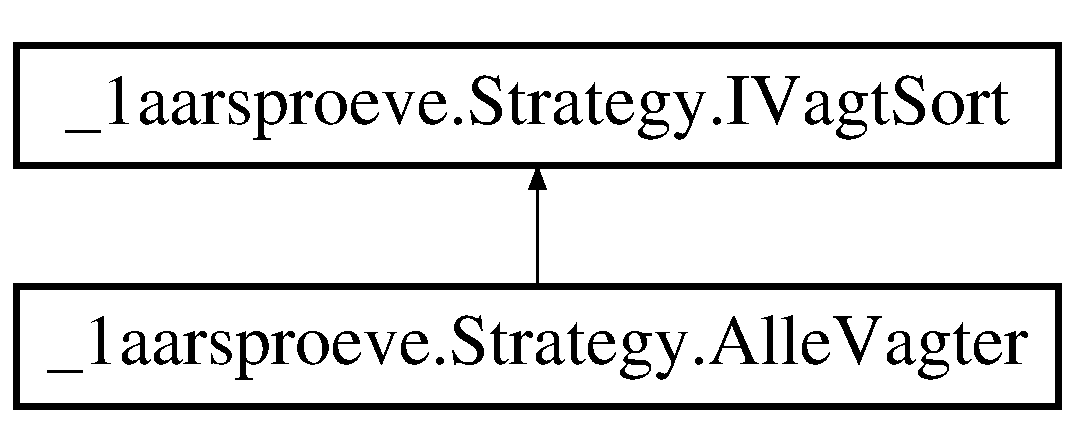
\includegraphics[height=2.000000cm]{class__1aarsproeve_1_1_strategy_1_1_alle_vagter}
\end{center}
\end{figure}
\subsection*{Public Member Functions}
\begin{DoxyCompactItemize}
\item 
async void \hyperlink{class__1aarsproeve_1_1_strategy_1_1_alle_vagter_a9155c0b6d6353e51c7e9d7c5a926c3f5}{Sort} (Observable\+Collection$<$ Observable\+Collection$<$ \hyperlink{class__1aarsproeve_1_1_model_1_1_vagtplan_view}{Vagtplan\+View} $>$$>$ vagt\+Collection, int ugenummer)
\begin{DoxyCompactList}\small\item\em Sorterer vagterne udfra Mine vagter \end{DoxyCompactList}\end{DoxyCompactItemize}


\subsection{Detailed Description}
\hyperlink{namespace__1aarsproeve_1_1_strategy}{Strategy} klasse der implmenterer \hyperlink{interface__1aarsproeve_1_1_strategy_1_1_i_vagt_sort}{I\+Vagt\+Sort} interfacet 



\subsection{Member Function Documentation}
\hypertarget{class__1aarsproeve_1_1_strategy_1_1_alle_vagter_a9155c0b6d6353e51c7e9d7c5a926c3f5}{}\index{\+\_\+1aarsproeve\+::\+Strategy\+::\+Alle\+Vagter@{\+\_\+1aarsproeve\+::\+Strategy\+::\+Alle\+Vagter}!Sort@{Sort}}
\index{Sort@{Sort}!\+\_\+1aarsproeve\+::\+Strategy\+::\+Alle\+Vagter@{\+\_\+1aarsproeve\+::\+Strategy\+::\+Alle\+Vagter}}
\subsubsection[{Sort}]{\setlength{\rightskip}{0pt plus 5cm}async void \+\_\+1aarsproeve.\+Strategy.\+Alle\+Vagter.\+Sort (
\begin{DoxyParamCaption}
\item[{Observable\+Collection$<$ Observable\+Collection$<$ {\bf Vagtplan\+View} $>$$>$}]{vagt\+Collection, }
\item[{int}]{ugenummer}
\end{DoxyParamCaption}
)}\label{class__1aarsproeve_1_1_strategy_1_1_alle_vagter_a9155c0b6d6353e51c7e9d7c5a926c3f5}


Sorterer vagterne udfra Mine vagter 


\begin{DoxyParams}{Parameters}
{\em vagt\+Collection} & Angiver hvilken collection der skal sorteres\\
\hline
{\em ugenummer} & Angiver for hvilken uge vagterne skal vises i\\
\hline
\end{DoxyParams}


Implements \hyperlink{interface__1aarsproeve_1_1_strategy_1_1_i_vagt_sort}{\+\_\+1aarsproeve.\+Strategy.\+I\+Vagt\+Sort}.



The documentation for this class was generated from the following file\+:\begin{DoxyCompactItemize}
\item 
Documents/\+Git\+Hub/1-\/aarsproeve/1aarsproeve/1aarsproeve/\+Strategy/Alle\+Vagter.\+cs\end{DoxyCompactItemize}

\hypertarget{class_w_s1aarsproeve_1_1_ansatte}{}\section{W\+S1aarsproeve.\+Ansatte Class Reference}
\label{class_w_s1aarsproeve_1_1_ansatte}\index{W\+S1aarsproeve.\+Ansatte@{W\+S1aarsproeve.\+Ansatte}}
\subsection*{Properties}
\begin{DoxyCompactItemize}
\item 
\hypertarget{class_w_s1aarsproeve_1_1_ansatte_af4eea3ca86ceb554b5379e819e5e1564}{}string {\bfseries Brugernavn}\hspace{0.3cm}{\ttfamily  \mbox{[}get, set\mbox{]}}\label{class_w_s1aarsproeve_1_1_ansatte_af4eea3ca86ceb554b5379e819e5e1564}

\item 
\hypertarget{class_w_s1aarsproeve_1_1_ansatte_a46767e24a97cd4f5048b2929a9dee858}{}string {\bfseries Navn}\hspace{0.3cm}{\ttfamily  \mbox{[}get, set\mbox{]}}\label{class_w_s1aarsproeve_1_1_ansatte_a46767e24a97cd4f5048b2929a9dee858}

\item 
\hypertarget{class_w_s1aarsproeve_1_1_ansatte_a993ef3da1ee00cee437aac73da154362}{}string {\bfseries Password}\hspace{0.3cm}{\ttfamily  \mbox{[}get, set\mbox{]}}\label{class_w_s1aarsproeve_1_1_ansatte_a993ef3da1ee00cee437aac73da154362}

\item 
\hypertarget{class_w_s1aarsproeve_1_1_ansatte_ac33e040e05f6bf10fef16985ab886d67}{}string {\bfseries Email}\hspace{0.3cm}{\ttfamily  \mbox{[}get, set\mbox{]}}\label{class_w_s1aarsproeve_1_1_ansatte_ac33e040e05f6bf10fef16985ab886d67}

\item 
\hypertarget{class_w_s1aarsproeve_1_1_ansatte_ad646658e4bbcf23653b6199dadbff943}{}string {\bfseries Mobil}\hspace{0.3cm}{\ttfamily  \mbox{[}get, set\mbox{]}}\label{class_w_s1aarsproeve_1_1_ansatte_ad646658e4bbcf23653b6199dadbff943}

\item 
\hypertarget{class_w_s1aarsproeve_1_1_ansatte_a9fecfb7308fc5bee164415316f66d5e7}{}string {\bfseries Adresse}\hspace{0.3cm}{\ttfamily  \mbox{[}get, set\mbox{]}}\label{class_w_s1aarsproeve_1_1_ansatte_a9fecfb7308fc5bee164415316f66d5e7}

\item 
\hypertarget{class_w_s1aarsproeve_1_1_ansatte_a205fd244d9e5f8dad555c4719e850eeb}{}string {\bfseries Postnummer}\hspace{0.3cm}{\ttfamily  \mbox{[}get, set\mbox{]}}\label{class_w_s1aarsproeve_1_1_ansatte_a205fd244d9e5f8dad555c4719e850eeb}

\item 
\hypertarget{class_w_s1aarsproeve_1_1_ansatte_a14cb42b82f9aed30d90560db003c36d9}{}int {\bfseries Stilling\+Id}\hspace{0.3cm}{\ttfamily  \mbox{[}get, set\mbox{]}}\label{class_w_s1aarsproeve_1_1_ansatte_a14cb42b82f9aed30d90560db003c36d9}

\item 
\hypertarget{class_w_s1aarsproeve_1_1_ansatte_ab296a881eea7a397c6d884c3aeac3277}{}virtual I\+Collection$<$ \hyperlink{class_w_s1aarsproeve_1_1_anmodninger}{Anmodninger} $>$ {\bfseries Anmodningers}\hspace{0.3cm}{\ttfamily  \mbox{[}get, set\mbox{]}}\label{class_w_s1aarsproeve_1_1_ansatte_ab296a881eea7a397c6d884c3aeac3277}

\item 
\hypertarget{class_w_s1aarsproeve_1_1_ansatte_a9aab54458a75700f9f2d8a1153f21d6e}{}virtual \hyperlink{class_w_s1aarsproeve_1_1_stillinger}{Stillinger} {\bfseries Stillinger}\hspace{0.3cm}{\ttfamily  \mbox{[}get, set\mbox{]}}\label{class_w_s1aarsproeve_1_1_ansatte_a9aab54458a75700f9f2d8a1153f21d6e}

\item 
\hypertarget{class_w_s1aarsproeve_1_1_ansatte_a8bfae47fc31de8cdb80d5a9e2ee13e39}{}virtual I\+Collection$<$ \hyperlink{class_w_s1aarsproeve_1_1_beskeder}{Beskeder} $>$ {\bfseries Beskeders}\hspace{0.3cm}{\ttfamily  \mbox{[}get, set\mbox{]}}\label{class_w_s1aarsproeve_1_1_ansatte_a8bfae47fc31de8cdb80d5a9e2ee13e39}

\item 
\hypertarget{class_w_s1aarsproeve_1_1_ansatte_aac27c59f47c1fe2e694c33691bce0d39}{}virtual I\+Collection$<$ \hyperlink{class_w_s1aarsproeve_1_1_vagter}{Vagter} $>$ {\bfseries Vagters}\hspace{0.3cm}{\ttfamily  \mbox{[}get, set\mbox{]}}\label{class_w_s1aarsproeve_1_1_ansatte_aac27c59f47c1fe2e694c33691bce0d39}

\end{DoxyCompactItemize}


The documentation for this class was generated from the following file\+:\begin{DoxyCompactItemize}
\item 
Documents/\+Git\+Hub/1-\/aarsproeve/1aarsproeve/\+W\+S1aarsproeve/\+Models/Ansatte.\+cs\end{DoxyCompactItemize}

\hypertarget{class__1aarsproeve_1_1_model_1_1_ansatte}{}\section{\+\_\+1aarsproeve.\+Model.\+Ansatte Class Reference}
\label{class__1aarsproeve_1_1_model_1_1_ansatte}\index{\+\_\+1aarsproeve.\+Model.\+Ansatte@{\+\_\+1aarsproeve.\+Model.\+Ansatte}}


\hyperlink{class__1aarsproeve_1_1_model_1_1_ansatte}{Ansatte} klasse der holder styr p� systemets brugere  


\subsection*{Public Member Functions}
\begin{DoxyCompactItemize}
\item 
\hyperlink{class__1aarsproeve_1_1_model_1_1_ansatte_a6b44f756d338148fc8d60b02eb5de340}{Ansatte} (string brugernavn, string navn, string password, string email, string mobil, string adresse, string postnummer, int stilling\+Id)
\begin{DoxyCompactList}\small\item\em \hyperlink{class__1aarsproeve_1_1_model_1_1_ansatte}{Ansatte} klassens konstrutkur \end{DoxyCompactList}\item 
\hyperlink{class__1aarsproeve_1_1_model_1_1_ansatte_a9f1c132875a9d68bad2db2052e51e73c}{Ansatte} ()
\begin{DoxyCompactList}\small\item\em Default konstrukt�r \end{DoxyCompactList}\item 
\hypertarget{class__1aarsproeve_1_1_model_1_1_ansatte_a95f708733a36460456ef4ceba140be1c}{}void {\bfseries Check\+Password} (string password)\label{class__1aarsproeve_1_1_model_1_1_ansatte_a95f708733a36460456ef4ceba140be1c}

\item 
\hypertarget{class__1aarsproeve_1_1_model_1_1_ansatte_ab0d5d55cae0254ee37443d2b0e19a6b3}{}void {\bfseries Check\+Brugernavn} (string brugernavn)\label{class__1aarsproeve_1_1_model_1_1_ansatte_ab0d5d55cae0254ee37443d2b0e19a6b3}

\item 
\hypertarget{class__1aarsproeve_1_1_model_1_1_ansatte_aed98e5f3d7ffa94e5dc9852c4f4c0666}{}void {\bfseries Checknavn} (string navn)\label{class__1aarsproeve_1_1_model_1_1_ansatte_aed98e5f3d7ffa94e5dc9852c4f4c0666}

\item 
\hypertarget{class__1aarsproeve_1_1_model_1_1_ansatte_a91cb7cfaced2c1e01ed13609b7a1c2e5}{}void {\bfseries Check\+Email} (string email)\label{class__1aarsproeve_1_1_model_1_1_ansatte_a91cb7cfaced2c1e01ed13609b7a1c2e5}

\item 
\hypertarget{class__1aarsproeve_1_1_model_1_1_ansatte_ad3dd92e6f9de305ccdc1c08b58b26909}{}void {\bfseries Check\+Adresse} (string adresse)\label{class__1aarsproeve_1_1_model_1_1_ansatte_ad3dd92e6f9de305ccdc1c08b58b26909}

\item 
\hypertarget{class__1aarsproeve_1_1_model_1_1_ansatte_ae876e63c3daff9eb6ee0a94ba68c1de6}{}void {\bfseries Check\+Mobil} (string mobil)\label{class__1aarsproeve_1_1_model_1_1_ansatte_ae876e63c3daff9eb6ee0a94ba68c1de6}

\item 
\hypertarget{class__1aarsproeve_1_1_model_1_1_ansatte_a4d89ea67f91a9157f5fedc33dc03a9bb}{}void {\bfseries Check\+Postnummer} (string postnummer)\label{class__1aarsproeve_1_1_model_1_1_ansatte_a4d89ea67f91a9157f5fedc33dc03a9bb}

\item 
override string \hyperlink{class__1aarsproeve_1_1_model_1_1_ansatte_ac4090e69bb8174b69cabc65aebf657b1}{To\+String} ()
\begin{DoxyCompactList}\small\item\em Viser \hyperlink{class__1aarsproeve_1_1_model_1_1_ansatte}{Ansatte} \end{DoxyCompactList}\end{DoxyCompactItemize}
\subsection*{Properties}
\begin{DoxyCompactItemize}
\item 
string \hyperlink{class__1aarsproeve_1_1_model_1_1_ansatte_a44168d0933bfdb17be69125e6e24beef}{Brugernavn}\hspace{0.3cm}{\ttfamily  \mbox{[}get, set\mbox{]}}
\begin{DoxyCompactList}\small\item\em Brugernavn property \end{DoxyCompactList}\item 
\hypertarget{class__1aarsproeve_1_1_model_1_1_ansatte_aef979eb6676057d230f774ce98582388}{}string {\bfseries Navn}\hspace{0.3cm}{\ttfamily  \mbox{[}get, set\mbox{]}}\label{class__1aarsproeve_1_1_model_1_1_ansatte_aef979eb6676057d230f774ce98582388}

\item 
string \hyperlink{class__1aarsproeve_1_1_model_1_1_ansatte_a6a74db68ea45111409666ee260481844}{Password}\hspace{0.3cm}{\ttfamily  \mbox{[}get, set\mbox{]}}
\begin{DoxyCompactList}\small\item\em Password property \end{DoxyCompactList}\item 
string \hyperlink{class__1aarsproeve_1_1_model_1_1_ansatte_a623f4cae464b7029fc70b71f1a39ecf5}{Email}\hspace{0.3cm}{\ttfamily  \mbox{[}get, set\mbox{]}}
\begin{DoxyCompactList}\small\item\em Email property \end{DoxyCompactList}\item 
string \hyperlink{class__1aarsproeve_1_1_model_1_1_ansatte_a4667b3d8f6bed8f8a40b0ee28542bc99}{Mobil}\hspace{0.3cm}{\ttfamily  \mbox{[}get, set\mbox{]}}
\begin{DoxyCompactList}\small\item\em Mobil property \end{DoxyCompactList}\item 
string \hyperlink{class__1aarsproeve_1_1_model_1_1_ansatte_a382a69881694cb6359b373e1538d8089}{Adresse}\hspace{0.3cm}{\ttfamily  \mbox{[}get, set\mbox{]}}
\begin{DoxyCompactList}\small\item\em Adresse property \end{DoxyCompactList}\item 
string \hyperlink{class__1aarsproeve_1_1_model_1_1_ansatte_a0dddb70ee83e53b898464039ee4af1d7}{Postnummer}\hspace{0.3cm}{\ttfamily  \mbox{[}get, set\mbox{]}}
\begin{DoxyCompactList}\small\item\em Postnummer property \end{DoxyCompactList}\item 
int \hyperlink{class__1aarsproeve_1_1_model_1_1_ansatte_acc76312a334de51d5476ccac3ddb3d5f}{Stilling\+Id}\hspace{0.3cm}{\ttfamily  \mbox{[}get, set\mbox{]}}
\begin{DoxyCompactList}\small\item\em Stilling\+Id property \end{DoxyCompactList}\end{DoxyCompactItemize}


\subsection{Detailed Description}
\hyperlink{class__1aarsproeve_1_1_model_1_1_ansatte}{Ansatte} klasse der holder styr p� systemets brugere 



\subsection{Constructor \& Destructor Documentation}
\hypertarget{class__1aarsproeve_1_1_model_1_1_ansatte_a6b44f756d338148fc8d60b02eb5de340}{}\index{\+\_\+1aarsproeve\+::\+Model\+::\+Ansatte@{\+\_\+1aarsproeve\+::\+Model\+::\+Ansatte}!Ansatte@{Ansatte}}
\index{Ansatte@{Ansatte}!\+\_\+1aarsproeve\+::\+Model\+::\+Ansatte@{\+\_\+1aarsproeve\+::\+Model\+::\+Ansatte}}
\subsubsection[{Ansatte}]{\setlength{\rightskip}{0pt plus 5cm}\+\_\+1aarsproeve.\+Model.\+Ansatte.\+Ansatte (
\begin{DoxyParamCaption}
\item[{string}]{brugernavn, }
\item[{string}]{navn, }
\item[{string}]{password, }
\item[{string}]{email, }
\item[{string}]{mobil, }
\item[{string}]{adresse, }
\item[{string}]{postnummer, }
\item[{int}]{stilling\+Id}
\end{DoxyParamCaption}
)}\label{class__1aarsproeve_1_1_model_1_1_ansatte_a6b44f756d338148fc8d60b02eb5de340}


\hyperlink{class__1aarsproeve_1_1_model_1_1_ansatte}{Ansatte} klassens konstrutkur 


\begin{DoxyParams}{Parameters}
{\em brugernavn} & Brugernavn parameter\\
\hline
{\em navn} & Navn parameter\\
\hline
{\em password} & Password parameter\\
\hline
{\em email} & Email parameter\\
\hline
{\em mobil} & Mobil parameter\\
\hline
{\em adresse} & Adresse parameter\\
\hline
{\em postnummer} & Postnummer parameter\\
\hline
{\em stilling\+Id} & Stilling\+Id paratmeter\\
\hline
\end{DoxyParams}
\hypertarget{class__1aarsproeve_1_1_model_1_1_ansatte_a9f1c132875a9d68bad2db2052e51e73c}{}\index{\+\_\+1aarsproeve\+::\+Model\+::\+Ansatte@{\+\_\+1aarsproeve\+::\+Model\+::\+Ansatte}!Ansatte@{Ansatte}}
\index{Ansatte@{Ansatte}!\+\_\+1aarsproeve\+::\+Model\+::\+Ansatte@{\+\_\+1aarsproeve\+::\+Model\+::\+Ansatte}}
\subsubsection[{Ansatte}]{\setlength{\rightskip}{0pt plus 5cm}\+\_\+1aarsproeve.\+Model.\+Ansatte.\+Ansatte (
\begin{DoxyParamCaption}
{}
\end{DoxyParamCaption}
)}\label{class__1aarsproeve_1_1_model_1_1_ansatte_a9f1c132875a9d68bad2db2052e51e73c}


Default konstrukt�r 



\subsection{Member Function Documentation}
\hypertarget{class__1aarsproeve_1_1_model_1_1_ansatte_ac4090e69bb8174b69cabc65aebf657b1}{}\index{\+\_\+1aarsproeve\+::\+Model\+::\+Ansatte@{\+\_\+1aarsproeve\+::\+Model\+::\+Ansatte}!To\+String@{To\+String}}
\index{To\+String@{To\+String}!\+\_\+1aarsproeve\+::\+Model\+::\+Ansatte@{\+\_\+1aarsproeve\+::\+Model\+::\+Ansatte}}
\subsubsection[{To\+String}]{\setlength{\rightskip}{0pt plus 5cm}override string \+\_\+1aarsproeve.\+Model.\+Ansatte.\+To\+String (
\begin{DoxyParamCaption}
{}
\end{DoxyParamCaption}
)}\label{class__1aarsproeve_1_1_model_1_1_ansatte_ac4090e69bb8174b69cabc65aebf657b1}


Viser \hyperlink{class__1aarsproeve_1_1_model_1_1_ansatte}{Ansatte} 

\begin{DoxyReturn}{Returns}
Returnerer To\+String \hyperlink{class__1aarsproeve_1_1_model_1_1_ansatte}{Ansatte}
\end{DoxyReturn}


\subsection{Property Documentation}
\hypertarget{class__1aarsproeve_1_1_model_1_1_ansatte_a382a69881694cb6359b373e1538d8089}{}\index{\+\_\+1aarsproeve\+::\+Model\+::\+Ansatte@{\+\_\+1aarsproeve\+::\+Model\+::\+Ansatte}!Adresse@{Adresse}}
\index{Adresse@{Adresse}!\+\_\+1aarsproeve\+::\+Model\+::\+Ansatte@{\+\_\+1aarsproeve\+::\+Model\+::\+Ansatte}}
\subsubsection[{Adresse}]{\setlength{\rightskip}{0pt plus 5cm}string \+\_\+1aarsproeve.\+Model.\+Ansatte.\+Adresse\hspace{0.3cm}{\ttfamily [get]}, {\ttfamily [set]}}\label{class__1aarsproeve_1_1_model_1_1_ansatte_a382a69881694cb6359b373e1538d8089}


Adresse property 

\hypertarget{class__1aarsproeve_1_1_model_1_1_ansatte_a44168d0933bfdb17be69125e6e24beef}{}\index{\+\_\+1aarsproeve\+::\+Model\+::\+Ansatte@{\+\_\+1aarsproeve\+::\+Model\+::\+Ansatte}!Brugernavn@{Brugernavn}}
\index{Brugernavn@{Brugernavn}!\+\_\+1aarsproeve\+::\+Model\+::\+Ansatte@{\+\_\+1aarsproeve\+::\+Model\+::\+Ansatte}}
\subsubsection[{Brugernavn}]{\setlength{\rightskip}{0pt plus 5cm}string \+\_\+1aarsproeve.\+Model.\+Ansatte.\+Brugernavn\hspace{0.3cm}{\ttfamily [get]}, {\ttfamily [set]}}\label{class__1aarsproeve_1_1_model_1_1_ansatte_a44168d0933bfdb17be69125e6e24beef}


Brugernavn property 

\hypertarget{class__1aarsproeve_1_1_model_1_1_ansatte_a623f4cae464b7029fc70b71f1a39ecf5}{}\index{\+\_\+1aarsproeve\+::\+Model\+::\+Ansatte@{\+\_\+1aarsproeve\+::\+Model\+::\+Ansatte}!Email@{Email}}
\index{Email@{Email}!\+\_\+1aarsproeve\+::\+Model\+::\+Ansatte@{\+\_\+1aarsproeve\+::\+Model\+::\+Ansatte}}
\subsubsection[{Email}]{\setlength{\rightskip}{0pt plus 5cm}string \+\_\+1aarsproeve.\+Model.\+Ansatte.\+Email\hspace{0.3cm}{\ttfamily [get]}, {\ttfamily [set]}}\label{class__1aarsproeve_1_1_model_1_1_ansatte_a623f4cae464b7029fc70b71f1a39ecf5}


Email property 

\hypertarget{class__1aarsproeve_1_1_model_1_1_ansatte_a4667b3d8f6bed8f8a40b0ee28542bc99}{}\index{\+\_\+1aarsproeve\+::\+Model\+::\+Ansatte@{\+\_\+1aarsproeve\+::\+Model\+::\+Ansatte}!Mobil@{Mobil}}
\index{Mobil@{Mobil}!\+\_\+1aarsproeve\+::\+Model\+::\+Ansatte@{\+\_\+1aarsproeve\+::\+Model\+::\+Ansatte}}
\subsubsection[{Mobil}]{\setlength{\rightskip}{0pt plus 5cm}string \+\_\+1aarsproeve.\+Model.\+Ansatte.\+Mobil\hspace{0.3cm}{\ttfamily [get]}, {\ttfamily [set]}}\label{class__1aarsproeve_1_1_model_1_1_ansatte_a4667b3d8f6bed8f8a40b0ee28542bc99}


Mobil property 

\hypertarget{class__1aarsproeve_1_1_model_1_1_ansatte_a6a74db68ea45111409666ee260481844}{}\index{\+\_\+1aarsproeve\+::\+Model\+::\+Ansatte@{\+\_\+1aarsproeve\+::\+Model\+::\+Ansatte}!Password@{Password}}
\index{Password@{Password}!\+\_\+1aarsproeve\+::\+Model\+::\+Ansatte@{\+\_\+1aarsproeve\+::\+Model\+::\+Ansatte}}
\subsubsection[{Password}]{\setlength{\rightskip}{0pt plus 5cm}string \+\_\+1aarsproeve.\+Model.\+Ansatte.\+Password\hspace{0.3cm}{\ttfamily [get]}, {\ttfamily [set]}}\label{class__1aarsproeve_1_1_model_1_1_ansatte_a6a74db68ea45111409666ee260481844}


Password property 

\hypertarget{class__1aarsproeve_1_1_model_1_1_ansatte_a0dddb70ee83e53b898464039ee4af1d7}{}\index{\+\_\+1aarsproeve\+::\+Model\+::\+Ansatte@{\+\_\+1aarsproeve\+::\+Model\+::\+Ansatte}!Postnummer@{Postnummer}}
\index{Postnummer@{Postnummer}!\+\_\+1aarsproeve\+::\+Model\+::\+Ansatte@{\+\_\+1aarsproeve\+::\+Model\+::\+Ansatte}}
\subsubsection[{Postnummer}]{\setlength{\rightskip}{0pt plus 5cm}string \+\_\+1aarsproeve.\+Model.\+Ansatte.\+Postnummer\hspace{0.3cm}{\ttfamily [get]}, {\ttfamily [set]}}\label{class__1aarsproeve_1_1_model_1_1_ansatte_a0dddb70ee83e53b898464039ee4af1d7}


Postnummer property 

\hypertarget{class__1aarsproeve_1_1_model_1_1_ansatte_acc76312a334de51d5476ccac3ddb3d5f}{}\index{\+\_\+1aarsproeve\+::\+Model\+::\+Ansatte@{\+\_\+1aarsproeve\+::\+Model\+::\+Ansatte}!Stilling\+Id@{Stilling\+Id}}
\index{Stilling\+Id@{Stilling\+Id}!\+\_\+1aarsproeve\+::\+Model\+::\+Ansatte@{\+\_\+1aarsproeve\+::\+Model\+::\+Ansatte}}
\subsubsection[{Stilling\+Id}]{\setlength{\rightskip}{0pt plus 5cm}int \+\_\+1aarsproeve.\+Model.\+Ansatte.\+Stilling\+Id\hspace{0.3cm}{\ttfamily [get]}, {\ttfamily [set]}}\label{class__1aarsproeve_1_1_model_1_1_ansatte_acc76312a334de51d5476ccac3ddb3d5f}


Stilling\+Id property 



The documentation for this class was generated from the following file\+:\begin{DoxyCompactItemize}
\item 
Documents/\+Git\+Hub/1-\/aarsproeve/1aarsproeve/1aarsproeve/\+Model/Ansatte.\+cs\end{DoxyCompactItemize}

\hypertarget{class__1aarsproeve_web_service_1_1_ansatte}{}\section{\+\_\+1aarsproeve\+Web\+Service.\+Ansatte Class Reference}
\label{class__1aarsproeve_web_service_1_1_ansatte}\index{\+\_\+1aarsproeve\+Web\+Service.\+Ansatte@{\+\_\+1aarsproeve\+Web\+Service.\+Ansatte}}
\subsection*{Properties}
\begin{DoxyCompactItemize}
\item 
\hypertarget{class__1aarsproeve_web_service_1_1_ansatte_a266da49f2082cf1a36e5ffdb9d6619be}{}string {\bfseries Brugernavn}\hspace{0.3cm}{\ttfamily  \mbox{[}get, set\mbox{]}}\label{class__1aarsproeve_web_service_1_1_ansatte_a266da49f2082cf1a36e5ffdb9d6619be}

\item 
\hypertarget{class__1aarsproeve_web_service_1_1_ansatte_ae2cdae5ed4bf100d864a4e8df1ead535}{}string {\bfseries Navn}\hspace{0.3cm}{\ttfamily  \mbox{[}get, set\mbox{]}}\label{class__1aarsproeve_web_service_1_1_ansatte_ae2cdae5ed4bf100d864a4e8df1ead535}

\item 
\hypertarget{class__1aarsproeve_web_service_1_1_ansatte_aaa29d692377cdb4e95a2434d92e0ef74}{}string {\bfseries Password}\hspace{0.3cm}{\ttfamily  \mbox{[}get, set\mbox{]}}\label{class__1aarsproeve_web_service_1_1_ansatte_aaa29d692377cdb4e95a2434d92e0ef74}

\item 
\hypertarget{class__1aarsproeve_web_service_1_1_ansatte_adcc5f7a69dbcfe145f01e68771b0d7f6}{}string {\bfseries Email}\hspace{0.3cm}{\ttfamily  \mbox{[}get, set\mbox{]}}\label{class__1aarsproeve_web_service_1_1_ansatte_adcc5f7a69dbcfe145f01e68771b0d7f6}

\item 
\hypertarget{class__1aarsproeve_web_service_1_1_ansatte_a517535fd4683512adf0c47697582587d}{}string {\bfseries Mobil}\hspace{0.3cm}{\ttfamily  \mbox{[}get, set\mbox{]}}\label{class__1aarsproeve_web_service_1_1_ansatte_a517535fd4683512adf0c47697582587d}

\item 
\hypertarget{class__1aarsproeve_web_service_1_1_ansatte_af8d84043c25ddab0dd07b521a25da7b8}{}string {\bfseries Adresse}\hspace{0.3cm}{\ttfamily  \mbox{[}get, set\mbox{]}}\label{class__1aarsproeve_web_service_1_1_ansatte_af8d84043c25ddab0dd07b521a25da7b8}

\item 
\hypertarget{class__1aarsproeve_web_service_1_1_ansatte_ae3351561fa7a58903c41481e9d166ddb}{}string {\bfseries Postnummer}\hspace{0.3cm}{\ttfamily  \mbox{[}get, set\mbox{]}}\label{class__1aarsproeve_web_service_1_1_ansatte_ae3351561fa7a58903c41481e9d166ddb}

\item 
\hypertarget{class__1aarsproeve_web_service_1_1_ansatte_a182d7ddf57afa474ccd698625d05998c}{}int {\bfseries Stilling\+Id}\hspace{0.3cm}{\ttfamily  \mbox{[}get, set\mbox{]}}\label{class__1aarsproeve_web_service_1_1_ansatte_a182d7ddf57afa474ccd698625d05998c}

\item 
\hypertarget{class__1aarsproeve_web_service_1_1_ansatte_ad1ed087ad6af3c5739a70b5764ec985e}{}virtual \hyperlink{class__1aarsproeve_web_service_1_1_stillinger}{Stillinger} {\bfseries Stillinger}\hspace{0.3cm}{\ttfamily  \mbox{[}get, set\mbox{]}}\label{class__1aarsproeve_web_service_1_1_ansatte_ad1ed087ad6af3c5739a70b5764ec985e}

\item 
\hypertarget{class__1aarsproeve_web_service_1_1_ansatte_a136eda68e5100d221a2cedf4b92997bd}{}virtual I\+Collection$<$ \hyperlink{class__1aarsproeve_web_service_1_1_beskeder}{Beskeder} $>$ {\bfseries Beskeders}\hspace{0.3cm}{\ttfamily  \mbox{[}get, set\mbox{]}}\label{class__1aarsproeve_web_service_1_1_ansatte_a136eda68e5100d221a2cedf4b92997bd}

\item 
\hypertarget{class__1aarsproeve_web_service_1_1_ansatte_ae30384475f123f2f3b50af71be05934c}{}virtual I\+Collection$<$ \hyperlink{class__1aarsproeve_web_service_1_1_vagter}{Vagter} $>$ {\bfseries Vagters}\hspace{0.3cm}{\ttfamily  \mbox{[}get, set\mbox{]}}\label{class__1aarsproeve_web_service_1_1_ansatte_ae30384475f123f2f3b50af71be05934c}

\end{DoxyCompactItemize}


The documentation for this class was generated from the following file\+:\begin{DoxyCompactItemize}
\item 
Documents/\+Git\+Hub/1-\/aarsproeve/1aarsproeve/1aarsproeve\+Web\+Service/Ansatte.\+cs\end{DoxyCompactItemize}

\hypertarget{class__1aarsproeve_web_service_1_1_controllers_1_1_ansattes_controller}{}\section{\+\_\+1aarsproeve\+Web\+Service.\+Controllers.\+Ansattes\+Controller Class Reference}
\label{class__1aarsproeve_web_service_1_1_controllers_1_1_ansattes_controller}\index{\+\_\+1aarsproeve\+Web\+Service.\+Controllers.\+Ansattes\+Controller@{\+\_\+1aarsproeve\+Web\+Service.\+Controllers.\+Ansattes\+Controller}}
Inheritance diagram for \+\_\+1aarsproeve\+Web\+Service.\+Controllers.\+Ansattes\+Controller\+:\begin{figure}[H]
\begin{center}
\leavevmode
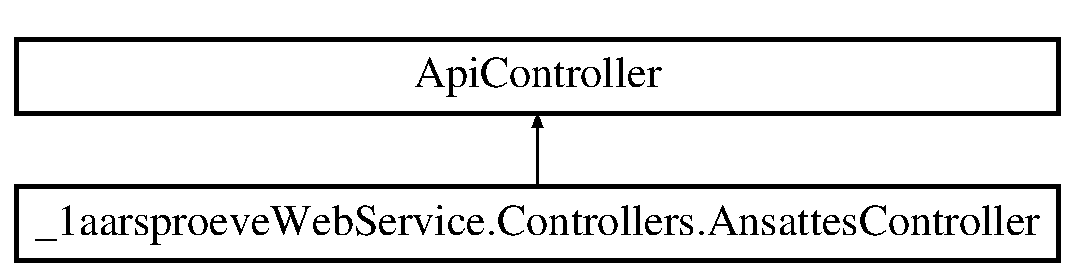
\includegraphics[height=2.000000cm]{class__1aarsproeve_web_service_1_1_controllers_1_1_ansattes_controller}
\end{center}
\end{figure}
\subsection*{Public Member Functions}
\begin{DoxyCompactItemize}
\item 
\hypertarget{class__1aarsproeve_web_service_1_1_controllers_1_1_ansattes_controller_a0f9b92dc8cf920494127741daa9f4f28}{}I\+Queryable$<$ \hyperlink{class__1aarsproeve_web_service_1_1_ansatte}{Ansatte} $>$ {\bfseries Get\+Ansattes} ()\label{class__1aarsproeve_web_service_1_1_controllers_1_1_ansattes_controller_a0f9b92dc8cf920494127741daa9f4f28}

\item 
\hypertarget{class__1aarsproeve_web_service_1_1_controllers_1_1_ansattes_controller_abfaf7e07989342482972410cfc37e38d}{}I\+Http\+Action\+Result {\bfseries Get\+Ansatte} (string id)\label{class__1aarsproeve_web_service_1_1_controllers_1_1_ansattes_controller_abfaf7e07989342482972410cfc37e38d}

\item 
\hypertarget{class__1aarsproeve_web_service_1_1_controllers_1_1_ansattes_controller_a038f479063bb013c0b522abe986c0214}{}I\+Http\+Action\+Result {\bfseries Put\+Ansatte} (string id, \hyperlink{class__1aarsproeve_web_service_1_1_ansatte}{Ansatte} ansatte)\label{class__1aarsproeve_web_service_1_1_controllers_1_1_ansattes_controller_a038f479063bb013c0b522abe986c0214}

\item 
\hypertarget{class__1aarsproeve_web_service_1_1_controllers_1_1_ansattes_controller_aef742593e8c9b738f375515b2a8e92c0}{}I\+Http\+Action\+Result {\bfseries Post\+Ansatte} (\hyperlink{class__1aarsproeve_web_service_1_1_ansatte}{Ansatte} ansatte)\label{class__1aarsproeve_web_service_1_1_controllers_1_1_ansattes_controller_aef742593e8c9b738f375515b2a8e92c0}

\item 
\hypertarget{class__1aarsproeve_web_service_1_1_controllers_1_1_ansattes_controller_a590c3bd2e247a51d547e53c47513b286}{}I\+Http\+Action\+Result {\bfseries Delete\+Ansatte} (string id)\label{class__1aarsproeve_web_service_1_1_controllers_1_1_ansattes_controller_a590c3bd2e247a51d547e53c47513b286}

\end{DoxyCompactItemize}
\subsection*{Protected Member Functions}
\begin{DoxyCompactItemize}
\item 
\hypertarget{class__1aarsproeve_web_service_1_1_controllers_1_1_ansattes_controller_ab4d04d1ad66ffdd3ab18b2276842fb2f}{}override void {\bfseries Dispose} (bool disposing)\label{class__1aarsproeve_web_service_1_1_controllers_1_1_ansattes_controller_ab4d04d1ad66ffdd3ab18b2276842fb2f}

\end{DoxyCompactItemize}


The documentation for this class was generated from the following file\+:\begin{DoxyCompactItemize}
\item 
Documents/\+Git\+Hub/1-\/aarsproeve/1aarsproeve/1aarsproeve\+Web\+Service/\+Controllers/Ansattes\+Controller.\+cs\end{DoxyCompactItemize}

\hypertarget{class_w_s1aarsproeve_1_1_controllers_1_1_ansattes_controller}{}\section{W\+S1aarsproeve.\+Controllers.\+Ansattes\+Controller Class Reference}
\label{class_w_s1aarsproeve_1_1_controllers_1_1_ansattes_controller}\index{W\+S1aarsproeve.\+Controllers.\+Ansattes\+Controller@{W\+S1aarsproeve.\+Controllers.\+Ansattes\+Controller}}
Inheritance diagram for W\+S1aarsproeve.\+Controllers.\+Ansattes\+Controller\+:\begin{figure}[H]
\begin{center}
\leavevmode
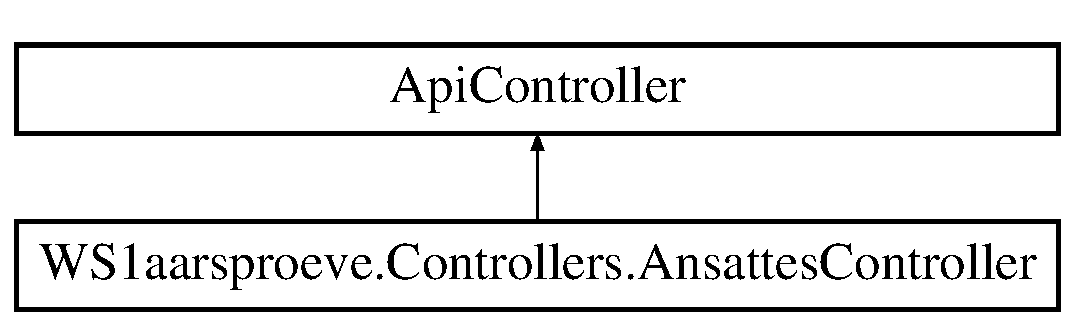
\includegraphics[height=2.000000cm]{class_w_s1aarsproeve_1_1_controllers_1_1_ansattes_controller}
\end{center}
\end{figure}
\subsection*{Public Member Functions}
\begin{DoxyCompactItemize}
\item 
\hypertarget{class_w_s1aarsproeve_1_1_controllers_1_1_ansattes_controller_abae1e97fe6c1da523b8282c16a60b004}{}I\+Queryable$<$ \hyperlink{class_w_s1aarsproeve_1_1_ansatte}{Ansatte} $>$ {\bfseries Get\+Ansattes} ()\label{class_w_s1aarsproeve_1_1_controllers_1_1_ansattes_controller_abae1e97fe6c1da523b8282c16a60b004}

\item 
\hypertarget{class_w_s1aarsproeve_1_1_controllers_1_1_ansattes_controller_a628a2903f9b4bdf4e73c4e3c5043c00f}{}I\+Http\+Action\+Result {\bfseries Get\+Ansatte} (string id)\label{class_w_s1aarsproeve_1_1_controllers_1_1_ansattes_controller_a628a2903f9b4bdf4e73c4e3c5043c00f}

\item 
\hypertarget{class_w_s1aarsproeve_1_1_controllers_1_1_ansattes_controller_a9b837cfedda7f79c523e5ce616e45837}{}I\+Http\+Action\+Result {\bfseries Put\+Ansatte} (string id, \hyperlink{class_w_s1aarsproeve_1_1_ansatte}{Ansatte} ansatte)\label{class_w_s1aarsproeve_1_1_controllers_1_1_ansattes_controller_a9b837cfedda7f79c523e5ce616e45837}

\item 
\hypertarget{class_w_s1aarsproeve_1_1_controllers_1_1_ansattes_controller_a64f55e5fa5fd3fd59b144eaee2bf1c00}{}I\+Http\+Action\+Result {\bfseries Post\+Ansatte} (\hyperlink{class_w_s1aarsproeve_1_1_ansatte}{Ansatte} ansatte)\label{class_w_s1aarsproeve_1_1_controllers_1_1_ansattes_controller_a64f55e5fa5fd3fd59b144eaee2bf1c00}

\item 
\hypertarget{class_w_s1aarsproeve_1_1_controllers_1_1_ansattes_controller_a64d601bd2f4d4d96728837179ed75a07}{}I\+Http\+Action\+Result {\bfseries Delete\+Ansatte} (string id)\label{class_w_s1aarsproeve_1_1_controllers_1_1_ansattes_controller_a64d601bd2f4d4d96728837179ed75a07}

\end{DoxyCompactItemize}
\subsection*{Protected Member Functions}
\begin{DoxyCompactItemize}
\item 
\hypertarget{class_w_s1aarsproeve_1_1_controllers_1_1_ansattes_controller_ad344ea6d5bca0dfbdc80e5cf1f06b2cc}{}override void {\bfseries Dispose} (bool disposing)\label{class_w_s1aarsproeve_1_1_controllers_1_1_ansattes_controller_ad344ea6d5bca0dfbdc80e5cf1f06b2cc}

\end{DoxyCompactItemize}


The documentation for this class was generated from the following file\+:\begin{DoxyCompactItemize}
\item 
Documents/\+Git\+Hub/1-\/aarsproeve/1aarsproeve/\+W\+S1aarsproeve/\+Controllers/Ansattes\+Controller.\+cs\end{DoxyCompactItemize}

\hypertarget{class__1aarsproeve_tests_1_1_ansatte_tests}{}\section{\+\_\+1aarsproeve\+Tests.\+Ansatte\+Tests Class Reference}
\label{class__1aarsproeve_tests_1_1_ansatte_tests}\index{\+\_\+1aarsproeve\+Tests.\+Ansatte\+Tests@{\+\_\+1aarsproeve\+Tests.\+Ansatte\+Tests}}
\subsection*{Public Member Functions}
\begin{DoxyCompactItemize}
\item 
\hypertarget{class__1aarsproeve_tests_1_1_ansatte_tests_a78f0ba95ff295255c876c20bc56156d1}{}void {\bfseries Before\+Test} ()\label{class__1aarsproeve_tests_1_1_ansatte_tests_a78f0ba95ff295255c876c20bc56156d1}

\item 
\hypertarget{class__1aarsproeve_tests_1_1_ansatte_tests_aa3ae94e496e0f0f03dc90fe4c8b68921}{}void {\bfseries Ansatte\+Test} ()\label{class__1aarsproeve_tests_1_1_ansatte_tests_aa3ae94e496e0f0f03dc90fe4c8b68921}

\item 
\hypertarget{class__1aarsproeve_tests_1_1_ansatte_tests_ac0f8f99fb21be1a1fe1f714013155779}{}void {\bfseries Ansatte\+Test1} ()\label{class__1aarsproeve_tests_1_1_ansatte_tests_ac0f8f99fb21be1a1fe1f714013155779}

\item 
\hypertarget{class__1aarsproeve_tests_1_1_ansatte_tests_ada5ece990b9338864cad5ea58bf2443f}{}void {\bfseries Ansatte\+Test2} ()\label{class__1aarsproeve_tests_1_1_ansatte_tests_ada5ece990b9338864cad5ea58bf2443f}

\item 
\hypertarget{class__1aarsproeve_tests_1_1_ansatte_tests_a597cb46674a2f7417bb9a61f821854a2}{}void {\bfseries Check\+Password\+Test} ()\label{class__1aarsproeve_tests_1_1_ansatte_tests_a597cb46674a2f7417bb9a61f821854a2}

\item 
\hypertarget{class__1aarsproeve_tests_1_1_ansatte_tests_aee8edf5afda59441655da5f9914fdecb}{}void {\bfseries Check\+Password\+Test1} ()\label{class__1aarsproeve_tests_1_1_ansatte_tests_aee8edf5afda59441655da5f9914fdecb}

\item 
\hypertarget{class__1aarsproeve_tests_1_1_ansatte_tests_acc2264dcd04cf2e86f71dc310f0b9bb8}{}void {\bfseries Check\+Password\+Test2} ()\label{class__1aarsproeve_tests_1_1_ansatte_tests_acc2264dcd04cf2e86f71dc310f0b9bb8}

\item 
\hypertarget{class__1aarsproeve_tests_1_1_ansatte_tests_af4df60f2061cc867f2f103d33d001b86}{}void {\bfseries Check\+Password\+Test3} ()\label{class__1aarsproeve_tests_1_1_ansatte_tests_af4df60f2061cc867f2f103d33d001b86}

\item 
\hypertarget{class__1aarsproeve_tests_1_1_ansatte_tests_a5d349d5ba9004f974c9757bc39a79941}{}void {\bfseries Check\+Brugernavn\+Test} ()\label{class__1aarsproeve_tests_1_1_ansatte_tests_a5d349d5ba9004f974c9757bc39a79941}

\item 
\hypertarget{class__1aarsproeve_tests_1_1_ansatte_tests_aa1dfe62618c136fac8445019719aa36e}{}void {\bfseries Check\+Brugernavn\+Test1} ()\label{class__1aarsproeve_tests_1_1_ansatte_tests_aa1dfe62618c136fac8445019719aa36e}

\item 
\hypertarget{class__1aarsproeve_tests_1_1_ansatte_tests_a06b50002be5bead45ad0d01c3bfac58d}{}void {\bfseries Check\+Brugernavn\+Test2} ()\label{class__1aarsproeve_tests_1_1_ansatte_tests_a06b50002be5bead45ad0d01c3bfac58d}

\item 
\hypertarget{class__1aarsproeve_tests_1_1_ansatte_tests_a56ebbba4296ff03bfb2edc9095313542}{}void {\bfseries Check\+Email\+Test} ()\label{class__1aarsproeve_tests_1_1_ansatte_tests_a56ebbba4296ff03bfb2edc9095313542}

\item 
\hypertarget{class__1aarsproeve_tests_1_1_ansatte_tests_ac61b9a93b89b21fc8cd467cf5daf1241}{}void {\bfseries Check\+Email\+Test1} ()\label{class__1aarsproeve_tests_1_1_ansatte_tests_ac61b9a93b89b21fc8cd467cf5daf1241}

\item 
\hypertarget{class__1aarsproeve_tests_1_1_ansatte_tests_a56f3bd9b75456b3cae05a34af642f022}{}void {\bfseries Check\+Email\+Test2} ()\label{class__1aarsproeve_tests_1_1_ansatte_tests_a56f3bd9b75456b3cae05a34af642f022}

\item 
\hypertarget{class__1aarsproeve_tests_1_1_ansatte_tests_ac42b90f037a311e917ca5eec0d99558f}{}void {\bfseries Check\+Adresse\+Test} ()\label{class__1aarsproeve_tests_1_1_ansatte_tests_ac42b90f037a311e917ca5eec0d99558f}

\item 
\hypertarget{class__1aarsproeve_tests_1_1_ansatte_tests_ab68f528f75994594e58ce7acf14cc672}{}void {\bfseries Check\+Adresse\+Test1} ()\label{class__1aarsproeve_tests_1_1_ansatte_tests_ab68f528f75994594e58ce7acf14cc672}

\item 
\hypertarget{class__1aarsproeve_tests_1_1_ansatte_tests_a117f78ffa10a1aa5a8cbf323226cded9}{}void {\bfseries Check\+Adresse\+Test2} ()\label{class__1aarsproeve_tests_1_1_ansatte_tests_a117f78ffa10a1aa5a8cbf323226cded9}

\item 
\hypertarget{class__1aarsproeve_tests_1_1_ansatte_tests_ab7a4369fd1c3b60be90c76683a176b7d}{}void {\bfseries Check\+Mobil\+Test} ()\label{class__1aarsproeve_tests_1_1_ansatte_tests_ab7a4369fd1c3b60be90c76683a176b7d}

\item 
\hypertarget{class__1aarsproeve_tests_1_1_ansatte_tests_a12b592d09f9d6486f20dcc772feae403}{}void {\bfseries Check\+Mobil\+Test1} ()\label{class__1aarsproeve_tests_1_1_ansatte_tests_a12b592d09f9d6486f20dcc772feae403}

\item 
\hypertarget{class__1aarsproeve_tests_1_1_ansatte_tests_a6363a57e892ba9531aeb65b5af268ee6}{}void {\bfseries Check\+Mobil\+Test3} ()\label{class__1aarsproeve_tests_1_1_ansatte_tests_a6363a57e892ba9531aeb65b5af268ee6}

\item 
\hypertarget{class__1aarsproeve_tests_1_1_ansatte_tests_a827601d9f74ac059f1e30ca38fbb5200}{}void {\bfseries Check\+Postnummer\+Test} ()\label{class__1aarsproeve_tests_1_1_ansatte_tests_a827601d9f74ac059f1e30ca38fbb5200}

\item 
\hypertarget{class__1aarsproeve_tests_1_1_ansatte_tests_a216a0fc13afc723d1fc7482da14d3ccd}{}void {\bfseries Check\+Post\+Test1} ()\label{class__1aarsproeve_tests_1_1_ansatte_tests_a216a0fc13afc723d1fc7482da14d3ccd}

\item 
\hypertarget{class__1aarsproeve_tests_1_1_ansatte_tests_a76d38b0a91fa1035532fbe186692a790}{}void {\bfseries Check\+Post\+Test3} ()\label{class__1aarsproeve_tests_1_1_ansatte_tests_a76d38b0a91fa1035532fbe186692a790}

\end{DoxyCompactItemize}


The documentation for this class was generated from the following file\+:\begin{DoxyCompactItemize}
\item 
Documents/\+Git\+Hub/1-\/aarsproeve/1aarsproeve/1aarsproeve\+Tests/Ansatte\+Tests.\+cs\end{DoxyCompactItemize}

\hypertarget{class__1aarsproeve_web_service_1_1_ansatte_view}{}\section{\+\_\+1aarsproeve\+Web\+Service.\+Ansatte\+View Class Reference}
\label{class__1aarsproeve_web_service_1_1_ansatte_view}\index{\+\_\+1aarsproeve\+Web\+Service.\+Ansatte\+View@{\+\_\+1aarsproeve\+Web\+Service.\+Ansatte\+View}}
\subsection*{Properties}
\begin{DoxyCompactItemize}
\item 
\hypertarget{class__1aarsproeve_web_service_1_1_ansatte_view_a26c5ca4df2d1636e6f4d0a2f187d1606}{}string {\bfseries Brugernavn}\hspace{0.3cm}{\ttfamily  \mbox{[}get, set\mbox{]}}\label{class__1aarsproeve_web_service_1_1_ansatte_view_a26c5ca4df2d1636e6f4d0a2f187d1606}

\item 
\hypertarget{class__1aarsproeve_web_service_1_1_ansatte_view_a29779b6ab76e66ee6557b7d494898747}{}string {\bfseries Navn}\hspace{0.3cm}{\ttfamily  \mbox{[}get, set\mbox{]}}\label{class__1aarsproeve_web_service_1_1_ansatte_view_a29779b6ab76e66ee6557b7d494898747}

\item 
\hypertarget{class__1aarsproeve_web_service_1_1_ansatte_view_a7ee2ee14a91aaf9fba5da5fc5a1064af}{}string {\bfseries Password}\hspace{0.3cm}{\ttfamily  \mbox{[}get, set\mbox{]}}\label{class__1aarsproeve_web_service_1_1_ansatte_view_a7ee2ee14a91aaf9fba5da5fc5a1064af}

\item 
\hypertarget{class__1aarsproeve_web_service_1_1_ansatte_view_a30ebd80cb0f5eeac8bb3ad05a5ab38be}{}string {\bfseries Email}\hspace{0.3cm}{\ttfamily  \mbox{[}get, set\mbox{]}}\label{class__1aarsproeve_web_service_1_1_ansatte_view_a30ebd80cb0f5eeac8bb3ad05a5ab38be}

\item 
\hypertarget{class__1aarsproeve_web_service_1_1_ansatte_view_ae5d56dc63321921afccc34a9a991db13}{}string {\bfseries Mobil}\hspace{0.3cm}{\ttfamily  \mbox{[}get, set\mbox{]}}\label{class__1aarsproeve_web_service_1_1_ansatte_view_ae5d56dc63321921afccc34a9a991db13}

\item 
\hypertarget{class__1aarsproeve_web_service_1_1_ansatte_view_ad181f1e27f096319bf2f107a832bcae4}{}string {\bfseries Adresse}\hspace{0.3cm}{\ttfamily  \mbox{[}get, set\mbox{]}}\label{class__1aarsproeve_web_service_1_1_ansatte_view_ad181f1e27f096319bf2f107a832bcae4}

\item 
\hypertarget{class__1aarsproeve_web_service_1_1_ansatte_view_a4b8033532cdc6d411a2ed3afc852f22f}{}string {\bfseries Postnummer}\hspace{0.3cm}{\ttfamily  \mbox{[}get, set\mbox{]}}\label{class__1aarsproeve_web_service_1_1_ansatte_view_a4b8033532cdc6d411a2ed3afc852f22f}

\item 
\hypertarget{class__1aarsproeve_web_service_1_1_ansatte_view_a20efc44aba45f87d58986746a6c26d5c}{}int {\bfseries Stilling\+Id}\hspace{0.3cm}{\ttfamily  \mbox{[}get, set\mbox{]}}\label{class__1aarsproeve_web_service_1_1_ansatte_view_a20efc44aba45f87d58986746a6c26d5c}

\end{DoxyCompactItemize}


The documentation for this class was generated from the following file\+:\begin{DoxyCompactItemize}
\item 
Documents/\+Git\+Hub/1-\/aarsproeve/1aarsproeve/1aarsproeve\+Web\+Service/Ansatte\+View.\+cs\end{DoxyCompactItemize}

\hypertarget{class__1aarsproeve_1_1_app}{}\section{\+\_\+1aarsproeve.\+App Class Reference}
\label{class__1aarsproeve_1_1_app}\index{\+\_\+1aarsproeve.\+App@{\+\_\+1aarsproeve.\+App}}


Provides application-\/specific behavior to supplement the default Application class.  


Inheritance diagram for \+\_\+1aarsproeve.\+App\+:\begin{figure}[H]
\begin{center}
\leavevmode
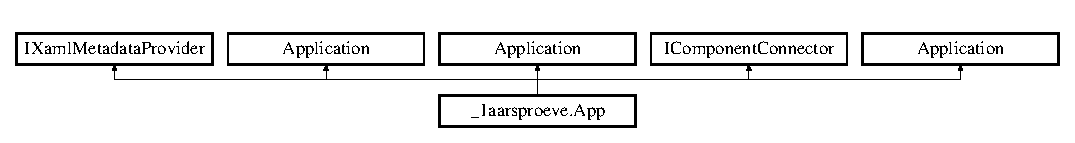
\includegraphics[height=1.473684cm]{class__1aarsproeve_1_1_app}
\end{center}
\end{figure}
\subsection*{Public Member Functions}
\begin{DoxyCompactItemize}
\item 
\hyperlink{class__1aarsproeve_1_1_app_a648545b697c46f7f879d3663198c24df}{App} ()
\begin{DoxyCompactList}\small\item\em Initializes the singleton application object. This is the first line of authored code executed, and as such is the logical equivalent of main() or Win\+Main(). \end{DoxyCompactList}\item 
\hypertarget{class__1aarsproeve_1_1_app_adeff2998728d62ed327627d0ac86916a}{}void {\bfseries Connect} (int connection\+Id, object target)\label{class__1aarsproeve_1_1_app_adeff2998728d62ed327627d0ac86916a}

\item 
\hypertarget{class__1aarsproeve_1_1_app_a3253c2995de585aac3f8db9e63fef8d5}{}void {\bfseries Initialize\+Component} ()\label{class__1aarsproeve_1_1_app_a3253c2995de585aac3f8db9e63fef8d5}

\item 
\hypertarget{class__1aarsproeve_1_1_app_a5114dc7c38ce1d6a07c6cf00fc555545}{}global\+::\+Windows.\+U\+I.\+Xaml.\+Markup.\+I\+Xaml\+Type {\bfseries Get\+Xaml\+Type} (global\+::\+System.\+Type type)\label{class__1aarsproeve_1_1_app_a5114dc7c38ce1d6a07c6cf00fc555545}

\item 
\hypertarget{class__1aarsproeve_1_1_app_a53d51c17fe7ca626f8eb7a25f6c24124}{}global\+::\+Windows.\+U\+I.\+Xaml.\+Markup.\+I\+Xaml\+Type {\bfseries Get\+Xaml\+Type} (string full\+Name)\label{class__1aarsproeve_1_1_app_a53d51c17fe7ca626f8eb7a25f6c24124}

\item 
\hypertarget{class__1aarsproeve_1_1_app_a9d2a8b1a028089c66bd83c91b1cc4528}{}global\+::\+Windows.\+U\+I.\+Xaml.\+Markup.\+Xmlns\+Definition\mbox{[}$\,$\mbox{]} {\bfseries Get\+Xmlns\+Definitions} ()\label{class__1aarsproeve_1_1_app_a9d2a8b1a028089c66bd83c91b1cc4528}

\end{DoxyCompactItemize}
\subsection*{Protected Member Functions}
\begin{DoxyCompactItemize}
\item 
override void \hyperlink{class__1aarsproeve_1_1_app_a1792d58bc636406fca229cf51ac6b81c}{On\+Launched} (Launch\+Activated\+Event\+Args e)
\begin{DoxyCompactList}\small\item\em Invoked when the application is launched normally by the end user. Other entry points will be used such as when the application is launched to open a specific file. \end{DoxyCompactList}\end{DoxyCompactItemize}


\subsection{Detailed Description}
Provides application-\/specific behavior to supplement the default Application class. 



\subsection{Constructor \& Destructor Documentation}
\hypertarget{class__1aarsproeve_1_1_app_a648545b697c46f7f879d3663198c24df}{}\index{\+\_\+1aarsproeve\+::\+App@{\+\_\+1aarsproeve\+::\+App}!App@{App}}
\index{App@{App}!\+\_\+1aarsproeve\+::\+App@{\+\_\+1aarsproeve\+::\+App}}
\subsubsection[{App}]{\setlength{\rightskip}{0pt plus 5cm}\+\_\+1aarsproeve.\+App.\+App (
\begin{DoxyParamCaption}
{}
\end{DoxyParamCaption}
)}\label{class__1aarsproeve_1_1_app_a648545b697c46f7f879d3663198c24df}


Initializes the singleton application object. This is the first line of authored code executed, and as such is the logical equivalent of main() or Win\+Main(). 



\subsection{Member Function Documentation}
\hypertarget{class__1aarsproeve_1_1_app_a1792d58bc636406fca229cf51ac6b81c}{}\index{\+\_\+1aarsproeve\+::\+App@{\+\_\+1aarsproeve\+::\+App}!On\+Launched@{On\+Launched}}
\index{On\+Launched@{On\+Launched}!\+\_\+1aarsproeve\+::\+App@{\+\_\+1aarsproeve\+::\+App}}
\subsubsection[{On\+Launched}]{\setlength{\rightskip}{0pt plus 5cm}override void \+\_\+1aarsproeve.\+App.\+On\+Launched (
\begin{DoxyParamCaption}
\item[{Launch\+Activated\+Event\+Args}]{e}
\end{DoxyParamCaption}
)\hspace{0.3cm}{\ttfamily [protected]}}\label{class__1aarsproeve_1_1_app_a1792d58bc636406fca229cf51ac6b81c}


Invoked when the application is launched normally by the end user. Other entry points will be used such as when the application is launched to open a specific file. 


\begin{DoxyParams}{Parameters}
{\em e} & Details about the launch request and process.\\
\hline
\end{DoxyParams}


The documentation for this class was generated from the following files\+:\begin{DoxyCompactItemize}
\item 
Documents/\+Git\+Hub/1-\/aarsproeve/1aarsproeve/1aarsproeve/App.\+xaml.\+cs\item 
Documents/\+Git\+Hub/1-\/aarsproeve/1aarsproeve/1aarsproeve/obj/\+Debug/App.\+g.\+i.\+cs\item 
Documents/\+Git\+Hub/1-\/aarsproeve/1aarsproeve/1aarsproeve/obj/\+Debug/Xaml\+Type\+Info.\+g.\+cs\item 
Documents/\+Git\+Hub/1-\/aarsproeve/1aarsproeve/1aarsproeve/obj/\+Debug/App.\+g.\+cs\end{DoxyCompactItemize}

\hypertarget{class_asp_child_control_type_attribute}{}\section{Asp\+Child\+Control\+Type\+Attribute Class Reference}
\label{class_asp_child_control_type_attribute}\index{Asp\+Child\+Control\+Type\+Attribute@{Asp\+Child\+Control\+Type\+Attribute}}
Inheritance diagram for Asp\+Child\+Control\+Type\+Attribute\+:\begin{figure}[H]
\begin{center}
\leavevmode
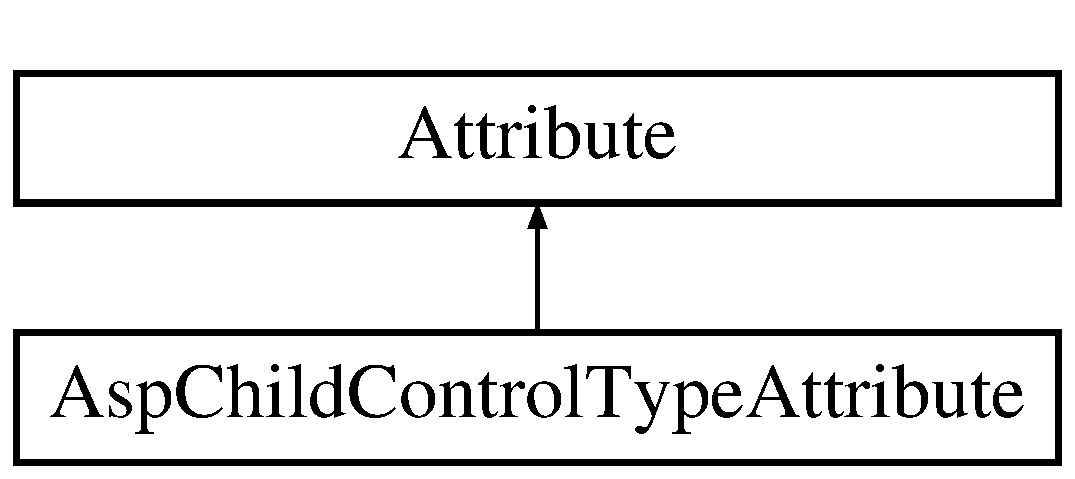
\includegraphics[height=2.000000cm]{class_asp_child_control_type_attribute}
\end{center}
\end{figure}
\subsection*{Public Member Functions}
\begin{DoxyCompactItemize}
\item 
\hypertarget{class_asp_child_control_type_attribute_ad547dcf065ac2d1092f0cce82cc26fe7}{}{\bfseries Asp\+Child\+Control\+Type\+Attribute} (string tag\+Name, Type control\+Type)\label{class_asp_child_control_type_attribute_ad547dcf065ac2d1092f0cce82cc26fe7}

\end{DoxyCompactItemize}
\subsection*{Properties}
\begin{DoxyCompactItemize}
\item 
\hypertarget{class_asp_child_control_type_attribute_a9e30613d70a3bcffb32a4664a5d121d2}{}string {\bfseries Tag\+Name}\hspace{0.3cm}{\ttfamily  \mbox{[}get\mbox{]}}\label{class_asp_child_control_type_attribute_a9e30613d70a3bcffb32a4664a5d121d2}

\item 
\hypertarget{class_asp_child_control_type_attribute_a6c6421f394baa882056b2dfc3efcd284}{}Type {\bfseries Control\+Type}\hspace{0.3cm}{\ttfamily  \mbox{[}get\mbox{]}}\label{class_asp_child_control_type_attribute_a6c6421f394baa882056b2dfc3efcd284}

\end{DoxyCompactItemize}


The documentation for this class was generated from the following file\+:\begin{DoxyCompactItemize}
\item 
Documents/\+Git\+Hub/1-\/aarsproeve/1aarsproeve/1aarsproeve/\+Properties/Annotations.\+cs\end{DoxyCompactItemize}

\hypertarget{class_asp_data_field_attribute}{}\section{Asp\+Data\+Field\+Attribute Class Reference}
\label{class_asp_data_field_attribute}\index{Asp\+Data\+Field\+Attribute@{Asp\+Data\+Field\+Attribute}}
Inheritance diagram for Asp\+Data\+Field\+Attribute\+:\begin{figure}[H]
\begin{center}
\leavevmode
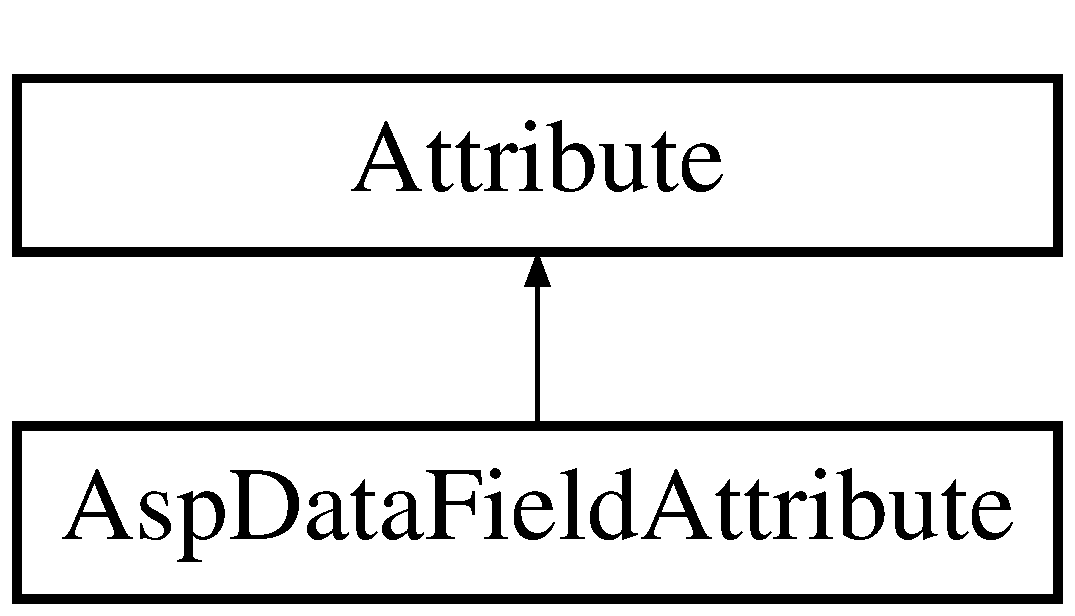
\includegraphics[height=2.000000cm]{class_asp_data_field_attribute}
\end{center}
\end{figure}


The documentation for this class was generated from the following file\+:\begin{DoxyCompactItemize}
\item 
Documents/\+Git\+Hub/1-\/aarsproeve/1aarsproeve/1aarsproeve/\+Properties/Annotations.\+cs\end{DoxyCompactItemize}

\hypertarget{class_asp_data_fields_attribute}{}\section{Asp\+Data\+Fields\+Attribute Class Reference}
\label{class_asp_data_fields_attribute}\index{Asp\+Data\+Fields\+Attribute@{Asp\+Data\+Fields\+Attribute}}
Inheritance diagram for Asp\+Data\+Fields\+Attribute\+:\begin{figure}[H]
\begin{center}
\leavevmode
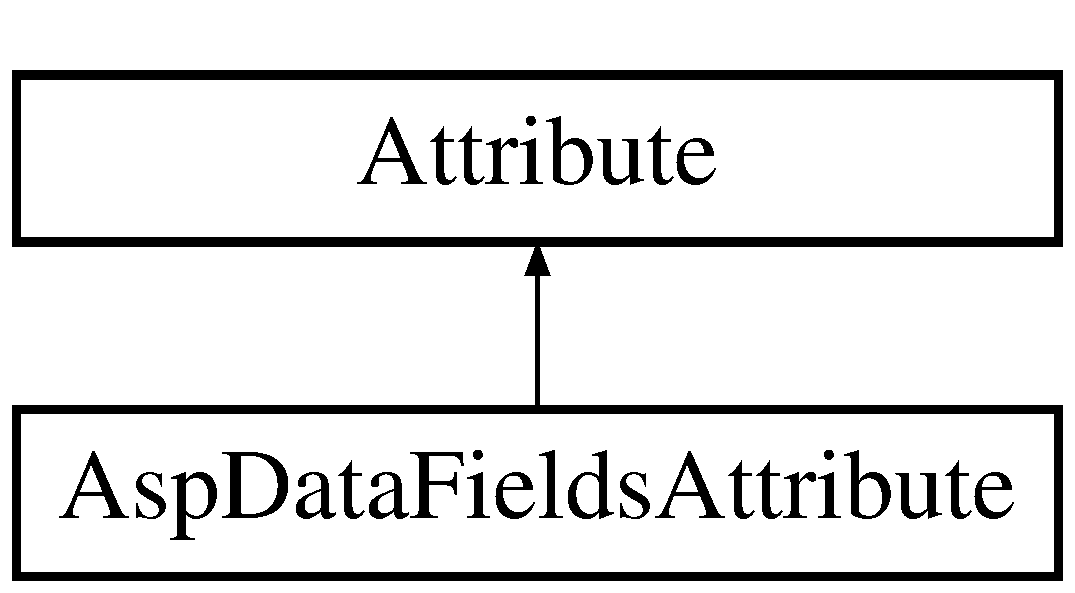
\includegraphics[height=2.000000cm]{class_asp_data_fields_attribute}
\end{center}
\end{figure}


The documentation for this class was generated from the following file\+:\begin{DoxyCompactItemize}
\item 
Documents/\+Git\+Hub/1-\/aarsproeve/1aarsproeve/1aarsproeve/\+Properties/Annotations.\+cs\end{DoxyCompactItemize}

\hypertarget{class_asp_method_property_attribute}{}\section{Asp\+Method\+Property\+Attribute Class Reference}
\label{class_asp_method_property_attribute}\index{Asp\+Method\+Property\+Attribute@{Asp\+Method\+Property\+Attribute}}
Inheritance diagram for Asp\+Method\+Property\+Attribute\+:\begin{figure}[H]
\begin{center}
\leavevmode
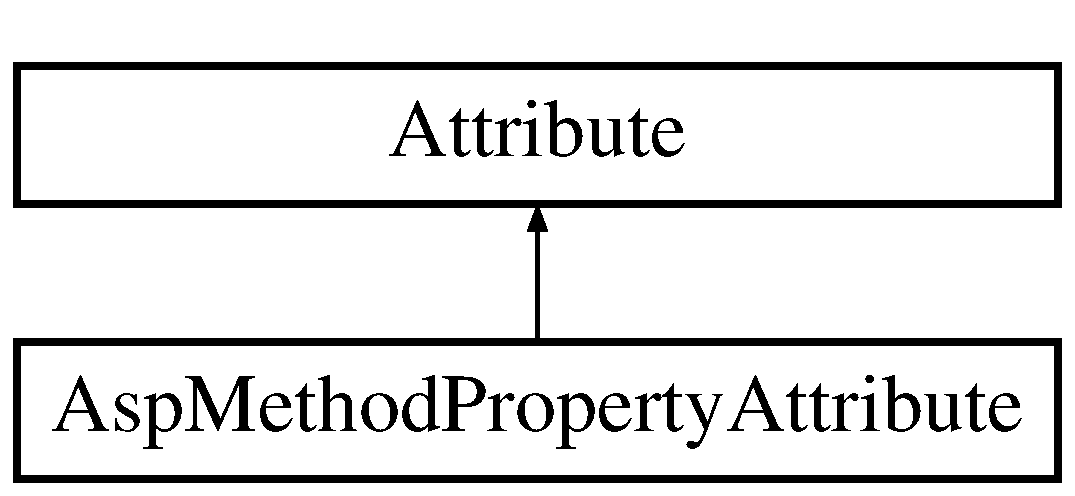
\includegraphics[height=2.000000cm]{class_asp_method_property_attribute}
\end{center}
\end{figure}


The documentation for this class was generated from the following file\+:\begin{DoxyCompactItemize}
\item 
Documents/\+Git\+Hub/1-\/aarsproeve/1aarsproeve/1aarsproeve/\+Properties/Annotations.\+cs\end{DoxyCompactItemize}

\hypertarget{class_asp_mvc_action_attribute}{}\section{Asp\+Mvc\+Action\+Attribute Class Reference}
\label{class_asp_mvc_action_attribute}\index{Asp\+Mvc\+Action\+Attribute@{Asp\+Mvc\+Action\+Attribute}}


A\+S\+P.\+N\+E\+T M\+V\+C attribute. If applied to a parameter, indicates that the parameter is an M\+V\+C action. If applied to a method, the M\+V\+C action name is calculated implicitly from the context. Use this attribute for custom wrappers similar to {\ttfamily System.\+Web.\+Mvc.\+Html.\+Child\+Action\+Extensions.\+Render\+Action(\+Html\+Helper, String)}  


Inheritance diagram for Asp\+Mvc\+Action\+Attribute\+:\begin{figure}[H]
\begin{center}
\leavevmode
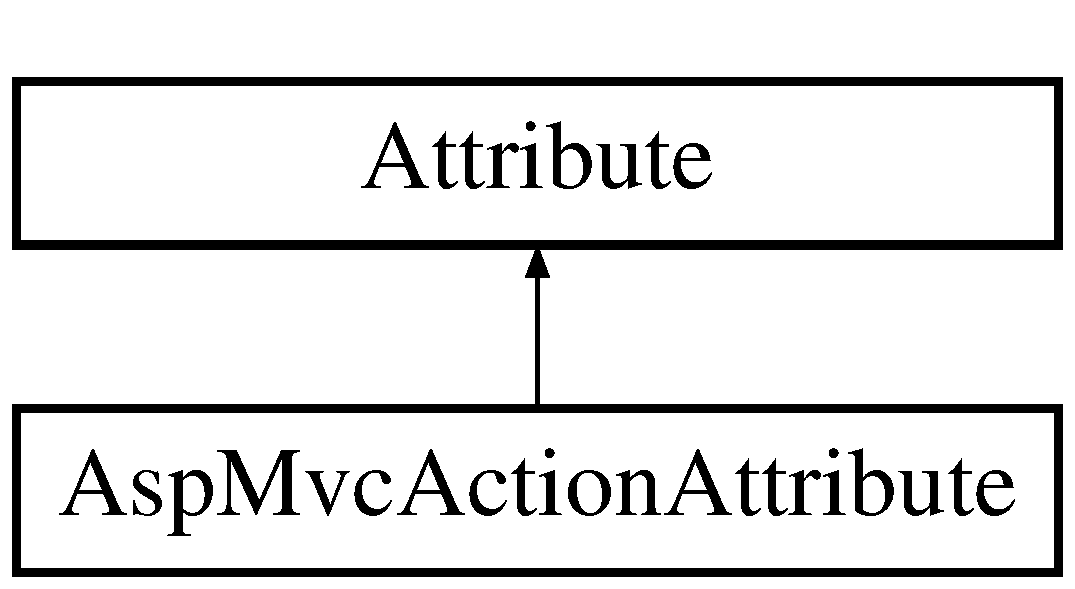
\includegraphics[height=2.000000cm]{class_asp_mvc_action_attribute}
\end{center}
\end{figure}
\subsection*{Public Member Functions}
\begin{DoxyCompactItemize}
\item 
\hypertarget{class_asp_mvc_action_attribute_a2f39095bf0a497897fbbc76e96621ff0}{}{\bfseries Asp\+Mvc\+Action\+Attribute} (string anonymous\+Property)\label{class_asp_mvc_action_attribute_a2f39095bf0a497897fbbc76e96621ff0}

\end{DoxyCompactItemize}
\subsection*{Properties}
\begin{DoxyCompactItemize}
\item 
\hypertarget{class_asp_mvc_action_attribute_a7068fa64becd1bc3de4622e5a50b0a49}{}string {\bfseries Anonymous\+Property}\hspace{0.3cm}{\ttfamily  \mbox{[}get\mbox{]}}\label{class_asp_mvc_action_attribute_a7068fa64becd1bc3de4622e5a50b0a49}

\end{DoxyCompactItemize}


\subsection{Detailed Description}
A\+S\+P.\+N\+E\+T M\+V\+C attribute. If applied to a parameter, indicates that the parameter is an M\+V\+C action. If applied to a method, the M\+V\+C action name is calculated implicitly from the context. Use this attribute for custom wrappers similar to {\ttfamily System.\+Web.\+Mvc.\+Html.\+Child\+Action\+Extensions.\+Render\+Action(\+Html\+Helper, String)} 



The documentation for this class was generated from the following file\+:\begin{DoxyCompactItemize}
\item 
Documents/\+Git\+Hub/1-\/aarsproeve/1aarsproeve/1aarsproeve/\+Properties/Annotations.\+cs\end{DoxyCompactItemize}

\hypertarget{class_asp_mvc_action_selector_attribute}{}\section{Asp\+Mvc\+Action\+Selector\+Attribute Class Reference}
\label{class_asp_mvc_action_selector_attribute}\index{Asp\+Mvc\+Action\+Selector\+Attribute@{Asp\+Mvc\+Action\+Selector\+Attribute}}


A\+S\+P.\+N\+E\+T M\+V\+C attribute. When applied to a parameter of an attribute, indicates that this parameter is an M\+V\+C action name  


Inheritance diagram for Asp\+Mvc\+Action\+Selector\+Attribute\+:\begin{figure}[H]
\begin{center}
\leavevmode
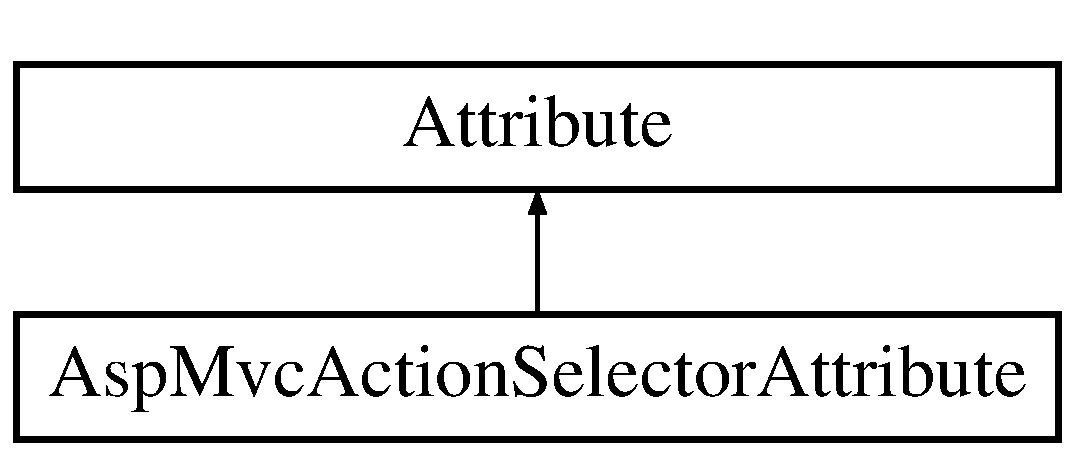
\includegraphics[height=2.000000cm]{class_asp_mvc_action_selector_attribute}
\end{center}
\end{figure}


\subsection{Detailed Description}
A\+S\+P.\+N\+E\+T M\+V\+C attribute. When applied to a parameter of an attribute, indicates that this parameter is an M\+V\+C action name 


\begin{DoxyCode}
[ActionName(\textcolor{stringliteral}{"Foo"})]
\textcolor{keyword}{public} ActionResult Login(\textcolor{keywordtype}{string} returnUrl) \{
  ViewBag.ReturnUrl = Url.Action(\textcolor{stringliteral}{"Foo"}); \textcolor{comment}{// OK}
  \textcolor{keywordflow}{return} RedirectToAction(\textcolor{stringliteral}{"Bar"}); \textcolor{comment}{// Error: Cannot resolve action}
\}
\end{DoxyCode}


The documentation for this class was generated from the following file\+:\begin{DoxyCompactItemize}
\item 
Documents/\+Git\+Hub/1-\/aarsproeve/1aarsproeve/1aarsproeve/\+Properties/Annotations.\+cs\end{DoxyCompactItemize}

\hypertarget{class_asp_mvc_area_attribute}{}\section{Asp\+Mvc\+Area\+Attribute Class Reference}
\label{class_asp_mvc_area_attribute}\index{Asp\+Mvc\+Area\+Attribute@{Asp\+Mvc\+Area\+Attribute}}


A\+S\+P.\+N\+E\+T M\+V\+C attribute. Indicates that a parameter is an M\+V\+C area. Use this attribute for custom wrappers similar to {\ttfamily System.\+Web.\+Mvc.\+Html.\+Child\+Action\+Extensions.\+Render\+Action(\+Html\+Helper, String)}  


Inheritance diagram for Asp\+Mvc\+Area\+Attribute\+:\begin{figure}[H]
\begin{center}
\leavevmode
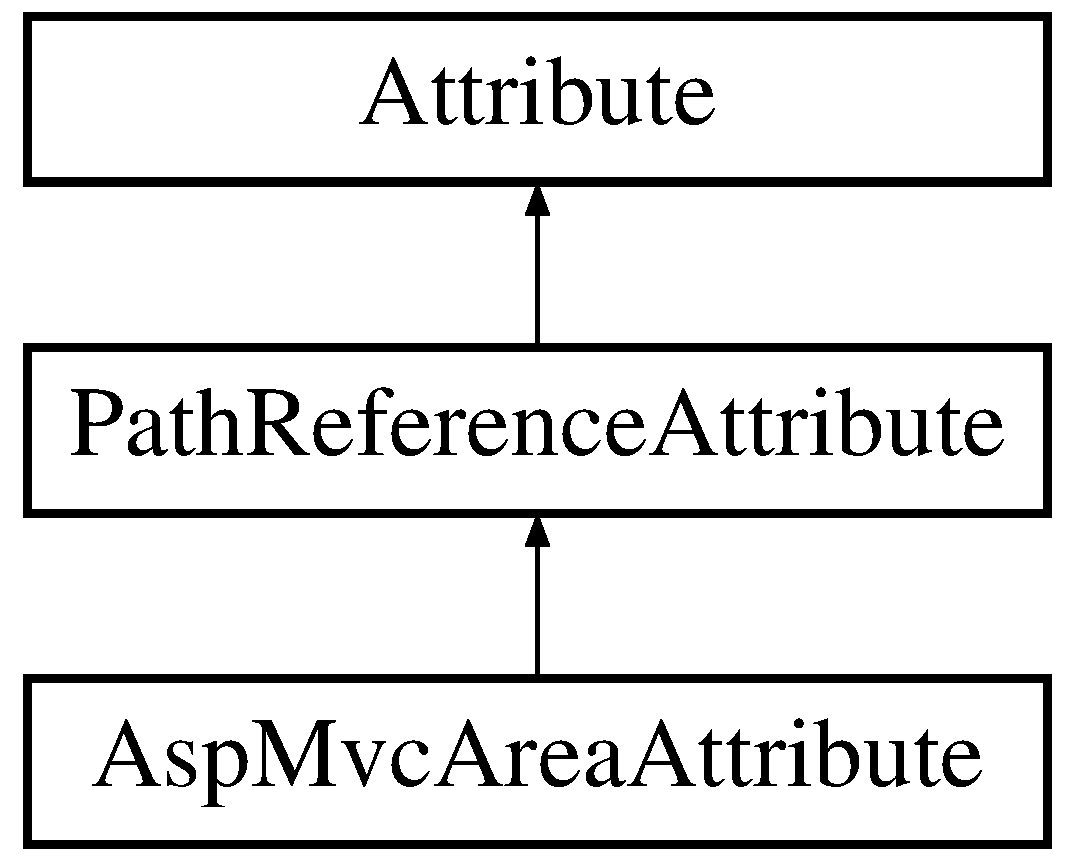
\includegraphics[height=3.000000cm]{class_asp_mvc_area_attribute}
\end{center}
\end{figure}
\subsection*{Public Member Functions}
\begin{DoxyCompactItemize}
\item 
\hypertarget{class_asp_mvc_area_attribute_ab0b90abe9b82844d54dd498623e0674e}{}{\bfseries Asp\+Mvc\+Area\+Attribute} (string anonymous\+Property)\label{class_asp_mvc_area_attribute_ab0b90abe9b82844d54dd498623e0674e}

\end{DoxyCompactItemize}
\subsection*{Properties}
\begin{DoxyCompactItemize}
\item 
\hypertarget{class_asp_mvc_area_attribute_a035e4e50658d154dfa22d68a08425a6b}{}string {\bfseries Anonymous\+Property}\hspace{0.3cm}{\ttfamily  \mbox{[}get\mbox{]}}\label{class_asp_mvc_area_attribute_a035e4e50658d154dfa22d68a08425a6b}

\end{DoxyCompactItemize}


\subsection{Detailed Description}
A\+S\+P.\+N\+E\+T M\+V\+C attribute. Indicates that a parameter is an M\+V\+C area. Use this attribute for custom wrappers similar to {\ttfamily System.\+Web.\+Mvc.\+Html.\+Child\+Action\+Extensions.\+Render\+Action(\+Html\+Helper, String)} 



The documentation for this class was generated from the following file\+:\begin{DoxyCompactItemize}
\item 
Documents/\+Git\+Hub/1-\/aarsproeve/1aarsproeve/1aarsproeve/\+Properties/Annotations.\+cs\end{DoxyCompactItemize}

\hypertarget{class_asp_mvc_area_master_location_format_attribute}{}\section{Asp\+Mvc\+Area\+Master\+Location\+Format\+Attribute Class Reference}
\label{class_asp_mvc_area_master_location_format_attribute}\index{Asp\+Mvc\+Area\+Master\+Location\+Format\+Attribute@{Asp\+Mvc\+Area\+Master\+Location\+Format\+Attribute}}
Inheritance diagram for Asp\+Mvc\+Area\+Master\+Location\+Format\+Attribute\+:\begin{figure}[H]
\begin{center}
\leavevmode
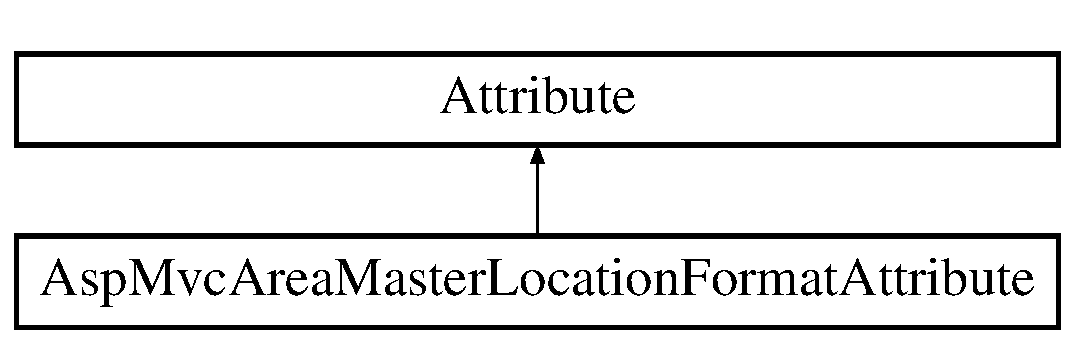
\includegraphics[height=2.000000cm]{class_asp_mvc_area_master_location_format_attribute}
\end{center}
\end{figure}
\subsection*{Public Member Functions}
\begin{DoxyCompactItemize}
\item 
\hypertarget{class_asp_mvc_area_master_location_format_attribute_ab46b99bdef3d52b97af74a67590c2aab}{}{\bfseries Asp\+Mvc\+Area\+Master\+Location\+Format\+Attribute} (string format)\label{class_asp_mvc_area_master_location_format_attribute_ab46b99bdef3d52b97af74a67590c2aab}

\end{DoxyCompactItemize}
\subsection*{Properties}
\begin{DoxyCompactItemize}
\item 
\hypertarget{class_asp_mvc_area_master_location_format_attribute_a4cb37b1a8f40ba0e5285cd1e602cf1c3}{}string {\bfseries Format}\hspace{0.3cm}{\ttfamily  \mbox{[}get\mbox{]}}\label{class_asp_mvc_area_master_location_format_attribute_a4cb37b1a8f40ba0e5285cd1e602cf1c3}

\end{DoxyCompactItemize}


The documentation for this class was generated from the following file\+:\begin{DoxyCompactItemize}
\item 
Documents/\+Git\+Hub/1-\/aarsproeve/1aarsproeve/1aarsproeve/\+Properties/Annotations.\+cs\end{DoxyCompactItemize}

\hypertarget{class_asp_mvc_area_partial_view_location_format_attribute}{}\section{Asp\+Mvc\+Area\+Partial\+View\+Location\+Format\+Attribute Class Reference}
\label{class_asp_mvc_area_partial_view_location_format_attribute}\index{Asp\+Mvc\+Area\+Partial\+View\+Location\+Format\+Attribute@{Asp\+Mvc\+Area\+Partial\+View\+Location\+Format\+Attribute}}
Inheritance diagram for Asp\+Mvc\+Area\+Partial\+View\+Location\+Format\+Attribute\+:\begin{figure}[H]
\begin{center}
\leavevmode
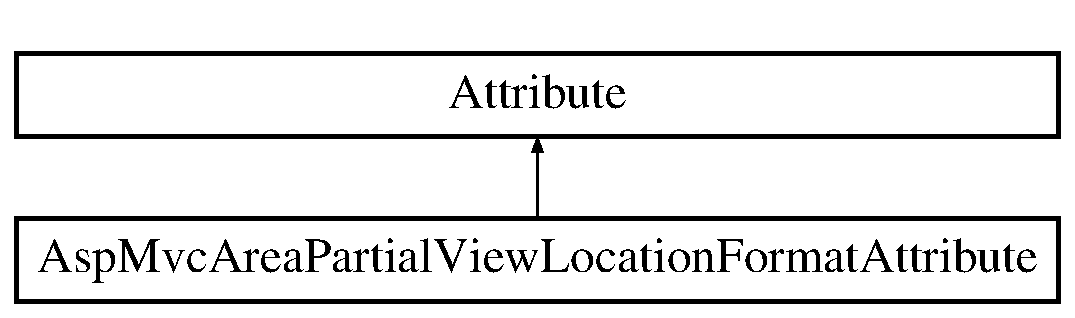
\includegraphics[height=2.000000cm]{class_asp_mvc_area_partial_view_location_format_attribute}
\end{center}
\end{figure}
\subsection*{Public Member Functions}
\begin{DoxyCompactItemize}
\item 
\hypertarget{class_asp_mvc_area_partial_view_location_format_attribute_a2cceb11c102f6ddf218094062d74b161}{}{\bfseries Asp\+Mvc\+Area\+Partial\+View\+Location\+Format\+Attribute} (string format)\label{class_asp_mvc_area_partial_view_location_format_attribute_a2cceb11c102f6ddf218094062d74b161}

\end{DoxyCompactItemize}
\subsection*{Properties}
\begin{DoxyCompactItemize}
\item 
\hypertarget{class_asp_mvc_area_partial_view_location_format_attribute_a9de8c471614445bbbcbf2051209ec446}{}string {\bfseries Format}\hspace{0.3cm}{\ttfamily  \mbox{[}get\mbox{]}}\label{class_asp_mvc_area_partial_view_location_format_attribute_a9de8c471614445bbbcbf2051209ec446}

\end{DoxyCompactItemize}


The documentation for this class was generated from the following file\+:\begin{DoxyCompactItemize}
\item 
Documents/\+Git\+Hub/1-\/aarsproeve/1aarsproeve/1aarsproeve/\+Properties/Annotations.\+cs\end{DoxyCompactItemize}

\hypertarget{class_asp_mvc_area_view_location_format_attribute}{}\section{Asp\+Mvc\+Area\+View\+Location\+Format\+Attribute Class Reference}
\label{class_asp_mvc_area_view_location_format_attribute}\index{Asp\+Mvc\+Area\+View\+Location\+Format\+Attribute@{Asp\+Mvc\+Area\+View\+Location\+Format\+Attribute}}
Inheritance diagram for Asp\+Mvc\+Area\+View\+Location\+Format\+Attribute\+:\begin{figure}[H]
\begin{center}
\leavevmode
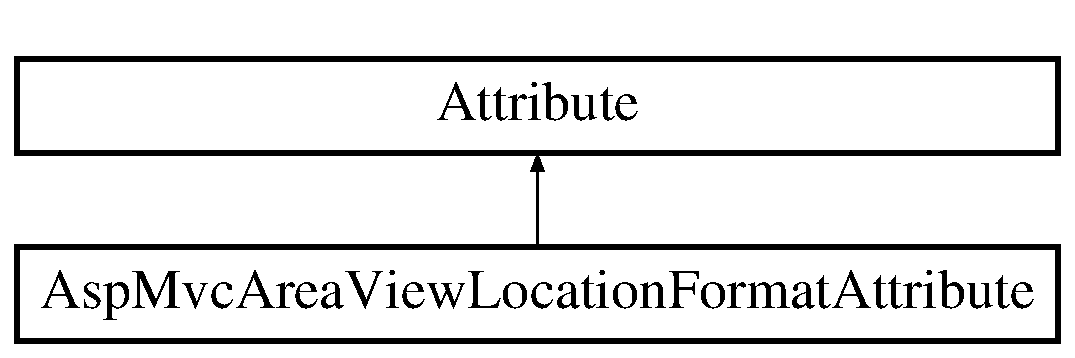
\includegraphics[height=2.000000cm]{class_asp_mvc_area_view_location_format_attribute}
\end{center}
\end{figure}
\subsection*{Public Member Functions}
\begin{DoxyCompactItemize}
\item 
\hypertarget{class_asp_mvc_area_view_location_format_attribute_a27bac0c5e55099e7d35be1f54f361a44}{}{\bfseries Asp\+Mvc\+Area\+View\+Location\+Format\+Attribute} (string format)\label{class_asp_mvc_area_view_location_format_attribute_a27bac0c5e55099e7d35be1f54f361a44}

\end{DoxyCompactItemize}
\subsection*{Properties}
\begin{DoxyCompactItemize}
\item 
\hypertarget{class_asp_mvc_area_view_location_format_attribute_ac3d03e8d1371c427048f84046c327e0e}{}string {\bfseries Format}\hspace{0.3cm}{\ttfamily  \mbox{[}get\mbox{]}}\label{class_asp_mvc_area_view_location_format_attribute_ac3d03e8d1371c427048f84046c327e0e}

\end{DoxyCompactItemize}


The documentation for this class was generated from the following file\+:\begin{DoxyCompactItemize}
\item 
Documents/\+Git\+Hub/1-\/aarsproeve/1aarsproeve/1aarsproeve/\+Properties/Annotations.\+cs\end{DoxyCompactItemize}

\hypertarget{class_asp_mvc_controller_attribute}{}\section{Asp\+Mvc\+Controller\+Attribute Class Reference}
\label{class_asp_mvc_controller_attribute}\index{Asp\+Mvc\+Controller\+Attribute@{Asp\+Mvc\+Controller\+Attribute}}


A\+S\+P.\+N\+E\+T M\+V\+C attribute. If applied to a parameter, indicates that the parameter is an M\+V\+C controller. If applied to a method, the M\+V\+C controller name is calculated implicitly from the context. Use this attribute for custom wrappers similar to {\ttfamily System.\+Web.\+Mvc.\+Html.\+Child\+Action\+Extensions.\+Render\+Action(\+Html\+Helper, String, String)}  


Inheritance diagram for Asp\+Mvc\+Controller\+Attribute\+:\begin{figure}[H]
\begin{center}
\leavevmode
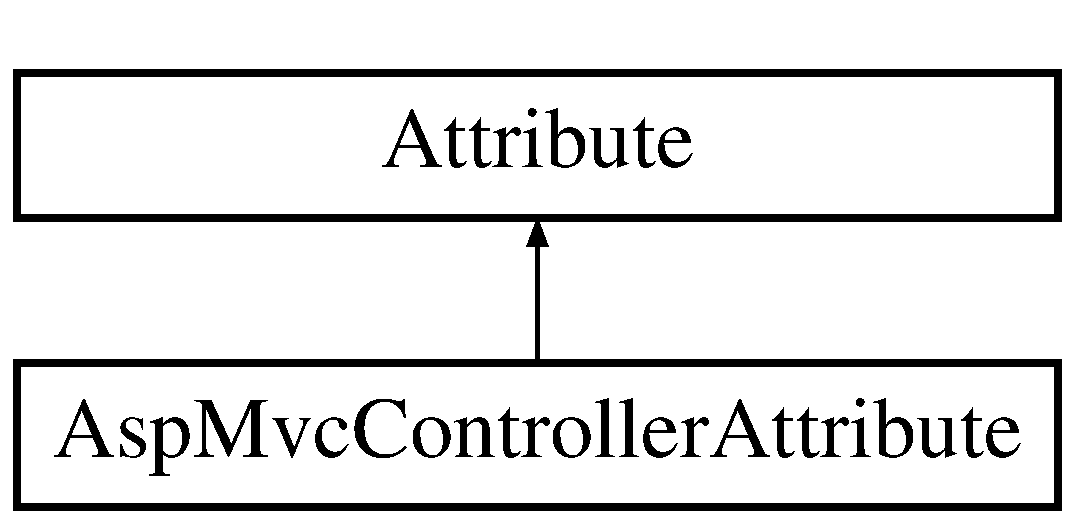
\includegraphics[height=2.000000cm]{class_asp_mvc_controller_attribute}
\end{center}
\end{figure}
\subsection*{Public Member Functions}
\begin{DoxyCompactItemize}
\item 
\hypertarget{class_asp_mvc_controller_attribute_a4e9eab92ec92d827df192a85b653f463}{}{\bfseries Asp\+Mvc\+Controller\+Attribute} (string anonymous\+Property)\label{class_asp_mvc_controller_attribute_a4e9eab92ec92d827df192a85b653f463}

\end{DoxyCompactItemize}
\subsection*{Properties}
\begin{DoxyCompactItemize}
\item 
\hypertarget{class_asp_mvc_controller_attribute_adb49d7099fe6a2366db45aca2e3488ab}{}string {\bfseries Anonymous\+Property}\hspace{0.3cm}{\ttfamily  \mbox{[}get\mbox{]}}\label{class_asp_mvc_controller_attribute_adb49d7099fe6a2366db45aca2e3488ab}

\end{DoxyCompactItemize}


\subsection{Detailed Description}
A\+S\+P.\+N\+E\+T M\+V\+C attribute. If applied to a parameter, indicates that the parameter is an M\+V\+C controller. If applied to a method, the M\+V\+C controller name is calculated implicitly from the context. Use this attribute for custom wrappers similar to {\ttfamily System.\+Web.\+Mvc.\+Html.\+Child\+Action\+Extensions.\+Render\+Action(\+Html\+Helper, String, String)} 



The documentation for this class was generated from the following file\+:\begin{DoxyCompactItemize}
\item 
Documents/\+Git\+Hub/1-\/aarsproeve/1aarsproeve/1aarsproeve/\+Properties/Annotations.\+cs\end{DoxyCompactItemize}

\hypertarget{class_asp_mvc_display_template_attribute}{}\section{Asp\+Mvc\+Display\+Template\+Attribute Class Reference}
\label{class_asp_mvc_display_template_attribute}\index{Asp\+Mvc\+Display\+Template\+Attribute@{Asp\+Mvc\+Display\+Template\+Attribute}}


A\+S\+P.\+N\+E\+T M\+V\+C attribute. Indicates that a parameter is an M\+V\+C display template. Use this attribute for custom wrappers similar to {\ttfamily System.\+Web.\+Mvc.\+Html.\+Display\+Extensions.\+Display\+For\+Model(\+Html\+Helper, String)}  


Inheritance diagram for Asp\+Mvc\+Display\+Template\+Attribute\+:\begin{figure}[H]
\begin{center}
\leavevmode
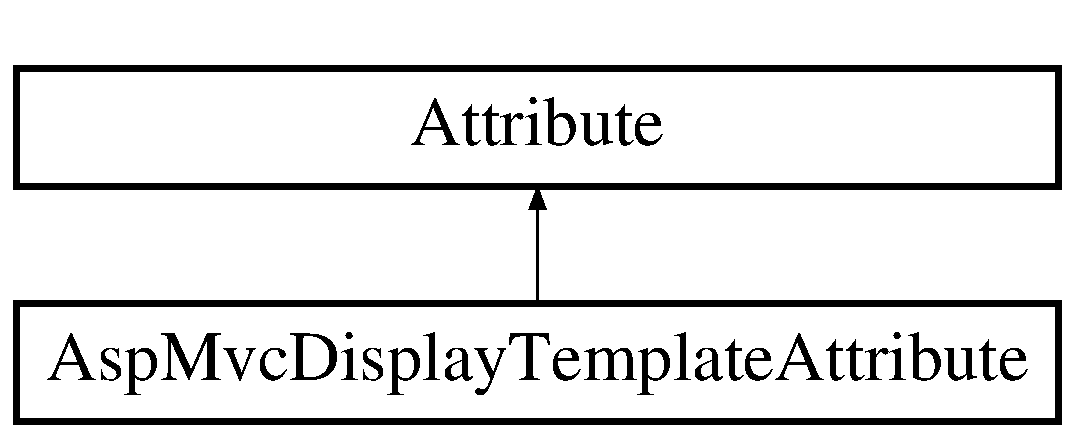
\includegraphics[height=2.000000cm]{class_asp_mvc_display_template_attribute}
\end{center}
\end{figure}


\subsection{Detailed Description}
A\+S\+P.\+N\+E\+T M\+V\+C attribute. Indicates that a parameter is an M\+V\+C display template. Use this attribute for custom wrappers similar to {\ttfamily System.\+Web.\+Mvc.\+Html.\+Display\+Extensions.\+Display\+For\+Model(\+Html\+Helper, String)} 



The documentation for this class was generated from the following file\+:\begin{DoxyCompactItemize}
\item 
Documents/\+Git\+Hub/1-\/aarsproeve/1aarsproeve/1aarsproeve/\+Properties/Annotations.\+cs\end{DoxyCompactItemize}

\hypertarget{class_asp_mvc_editor_template_attribute}{}\section{Asp\+Mvc\+Editor\+Template\+Attribute Class Reference}
\label{class_asp_mvc_editor_template_attribute}\index{Asp\+Mvc\+Editor\+Template\+Attribute@{Asp\+Mvc\+Editor\+Template\+Attribute}}


A\+S\+P.\+N\+E\+T M\+V\+C attribute. Indicates that a parameter is an M\+V\+C editor template. Use this attribute for custom wrappers similar to {\ttfamily System.\+Web.\+Mvc.\+Html.\+Editor\+Extensions.\+Editor\+For\+Model(\+Html\+Helper, String)}  


Inheritance diagram for Asp\+Mvc\+Editor\+Template\+Attribute\+:\begin{figure}[H]
\begin{center}
\leavevmode
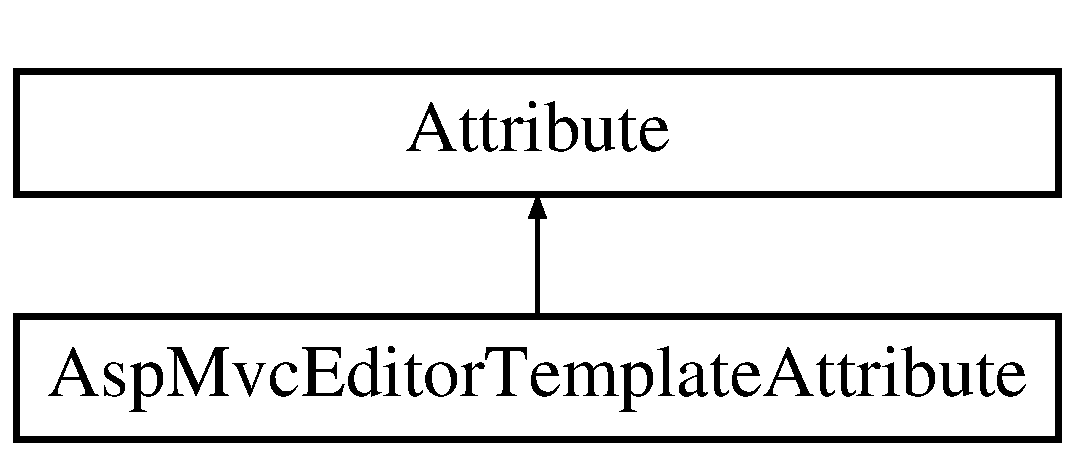
\includegraphics[height=2.000000cm]{class_asp_mvc_editor_template_attribute}
\end{center}
\end{figure}


\subsection{Detailed Description}
A\+S\+P.\+N\+E\+T M\+V\+C attribute. Indicates that a parameter is an M\+V\+C editor template. Use this attribute for custom wrappers similar to {\ttfamily System.\+Web.\+Mvc.\+Html.\+Editor\+Extensions.\+Editor\+For\+Model(\+Html\+Helper, String)} 



The documentation for this class was generated from the following file\+:\begin{DoxyCompactItemize}
\item 
Documents/\+Git\+Hub/1-\/aarsproeve/1aarsproeve/1aarsproeve/\+Properties/Annotations.\+cs\end{DoxyCompactItemize}

\hypertarget{class_asp_mvc_master_attribute}{}\section{Asp\+Mvc\+Master\+Attribute Class Reference}
\label{class_asp_mvc_master_attribute}\index{Asp\+Mvc\+Master\+Attribute@{Asp\+Mvc\+Master\+Attribute}}


A\+S\+P.\+N\+E\+T M\+V\+C attribute. Indicates that a parameter is an M\+V\+C Master. Use this attribute for custom wrappers similar to {\ttfamily System.\+Web.\+Mvc.\+Controller.\+View(\+String, String)}  


Inheritance diagram for Asp\+Mvc\+Master\+Attribute\+:\begin{figure}[H]
\begin{center}
\leavevmode
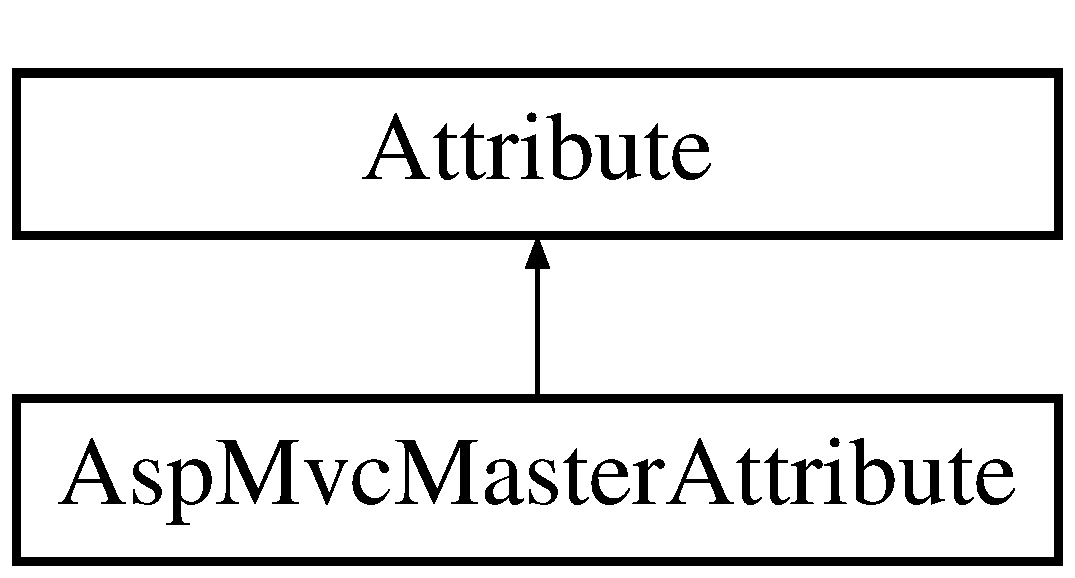
\includegraphics[height=2.000000cm]{class_asp_mvc_master_attribute}
\end{center}
\end{figure}


\subsection{Detailed Description}
A\+S\+P.\+N\+E\+T M\+V\+C attribute. Indicates that a parameter is an M\+V\+C Master. Use this attribute for custom wrappers similar to {\ttfamily System.\+Web.\+Mvc.\+Controller.\+View(\+String, String)} 



The documentation for this class was generated from the following file\+:\begin{DoxyCompactItemize}
\item 
Documents/\+Git\+Hub/1-\/aarsproeve/1aarsproeve/1aarsproeve/\+Properties/Annotations.\+cs\end{DoxyCompactItemize}

\hypertarget{class_asp_mvc_master_location_format_attribute}{}\section{Asp\+Mvc\+Master\+Location\+Format\+Attribute Class Reference}
\label{class_asp_mvc_master_location_format_attribute}\index{Asp\+Mvc\+Master\+Location\+Format\+Attribute@{Asp\+Mvc\+Master\+Location\+Format\+Attribute}}
Inheritance diagram for Asp\+Mvc\+Master\+Location\+Format\+Attribute\+:\begin{figure}[H]
\begin{center}
\leavevmode
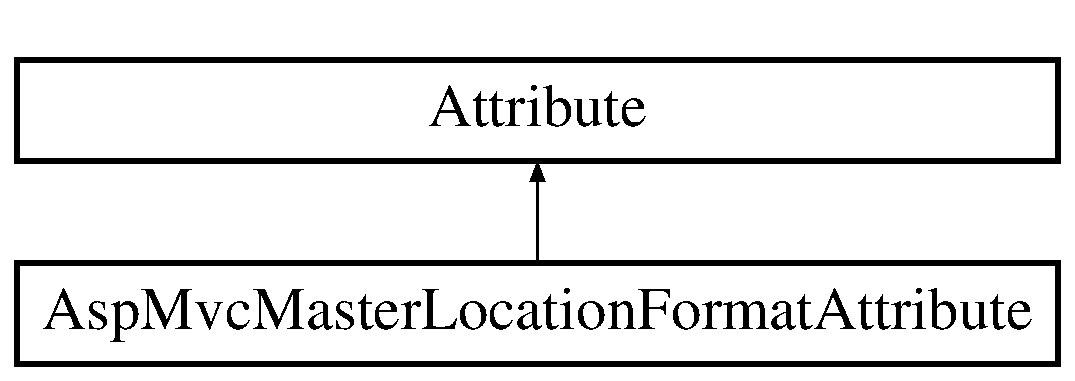
\includegraphics[height=2.000000cm]{class_asp_mvc_master_location_format_attribute}
\end{center}
\end{figure}
\subsection*{Public Member Functions}
\begin{DoxyCompactItemize}
\item 
\hypertarget{class_asp_mvc_master_location_format_attribute_ac71ce5737a8427494201b92935523fd9}{}{\bfseries Asp\+Mvc\+Master\+Location\+Format\+Attribute} (string format)\label{class_asp_mvc_master_location_format_attribute_ac71ce5737a8427494201b92935523fd9}

\end{DoxyCompactItemize}
\subsection*{Properties}
\begin{DoxyCompactItemize}
\item 
\hypertarget{class_asp_mvc_master_location_format_attribute_a12e48477c571f14556915ebdef251912}{}string {\bfseries Format}\hspace{0.3cm}{\ttfamily  \mbox{[}get\mbox{]}}\label{class_asp_mvc_master_location_format_attribute_a12e48477c571f14556915ebdef251912}

\end{DoxyCompactItemize}


The documentation for this class was generated from the following file\+:\begin{DoxyCompactItemize}
\item 
Documents/\+Git\+Hub/1-\/aarsproeve/1aarsproeve/1aarsproeve/\+Properties/Annotations.\+cs\end{DoxyCompactItemize}

\hypertarget{class_asp_mvc_model_type_attribute}{}\section{Asp\+Mvc\+Model\+Type\+Attribute Class Reference}
\label{class_asp_mvc_model_type_attribute}\index{Asp\+Mvc\+Model\+Type\+Attribute@{Asp\+Mvc\+Model\+Type\+Attribute}}


A\+S\+P.\+N\+E\+T M\+V\+C attribute. Indicates that a parameter is an M\+V\+C model type. Use this attribute for custom wrappers similar to {\ttfamily System.\+Web.\+Mvc.\+Controller.\+View(\+String, Object)}  


Inheritance diagram for Asp\+Mvc\+Model\+Type\+Attribute\+:\begin{figure}[H]
\begin{center}
\leavevmode
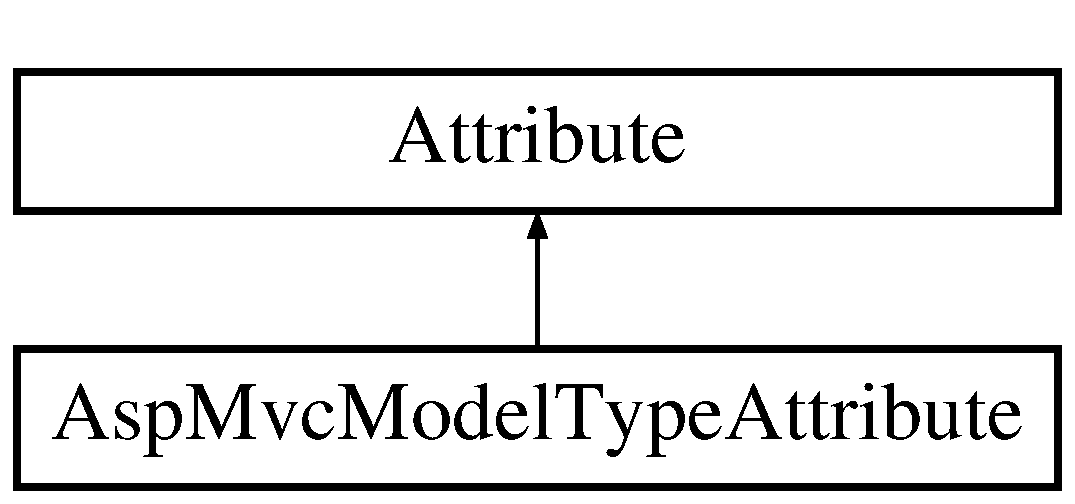
\includegraphics[height=2.000000cm]{class_asp_mvc_model_type_attribute}
\end{center}
\end{figure}


\subsection{Detailed Description}
A\+S\+P.\+N\+E\+T M\+V\+C attribute. Indicates that a parameter is an M\+V\+C model type. Use this attribute for custom wrappers similar to {\ttfamily System.\+Web.\+Mvc.\+Controller.\+View(\+String, Object)} 



The documentation for this class was generated from the following file\+:\begin{DoxyCompactItemize}
\item 
Documents/\+Git\+Hub/1-\/aarsproeve/1aarsproeve/1aarsproeve/\+Properties/Annotations.\+cs\end{DoxyCompactItemize}

\hypertarget{class_asp_mvc_partial_view_attribute}{}\section{Asp\+Mvc\+Partial\+View\+Attribute Class Reference}
\label{class_asp_mvc_partial_view_attribute}\index{Asp\+Mvc\+Partial\+View\+Attribute@{Asp\+Mvc\+Partial\+View\+Attribute}}


A\+S\+P.\+N\+E\+T M\+V\+C attribute. If applied to a parameter, indicates that the parameter is an M\+V\+C partial view. If applied to a method, the M\+V\+C partial view name is calculated implicitly from the context. Use this attribute for custom wrappers similar to {\ttfamily System.\+Web.\+Mvc.\+Html.\+Render\+Partial\+Extensions.\+Render\+Partial(\+Html\+Helper, String)}  


Inheritance diagram for Asp\+Mvc\+Partial\+View\+Attribute\+:\begin{figure}[H]
\begin{center}
\leavevmode
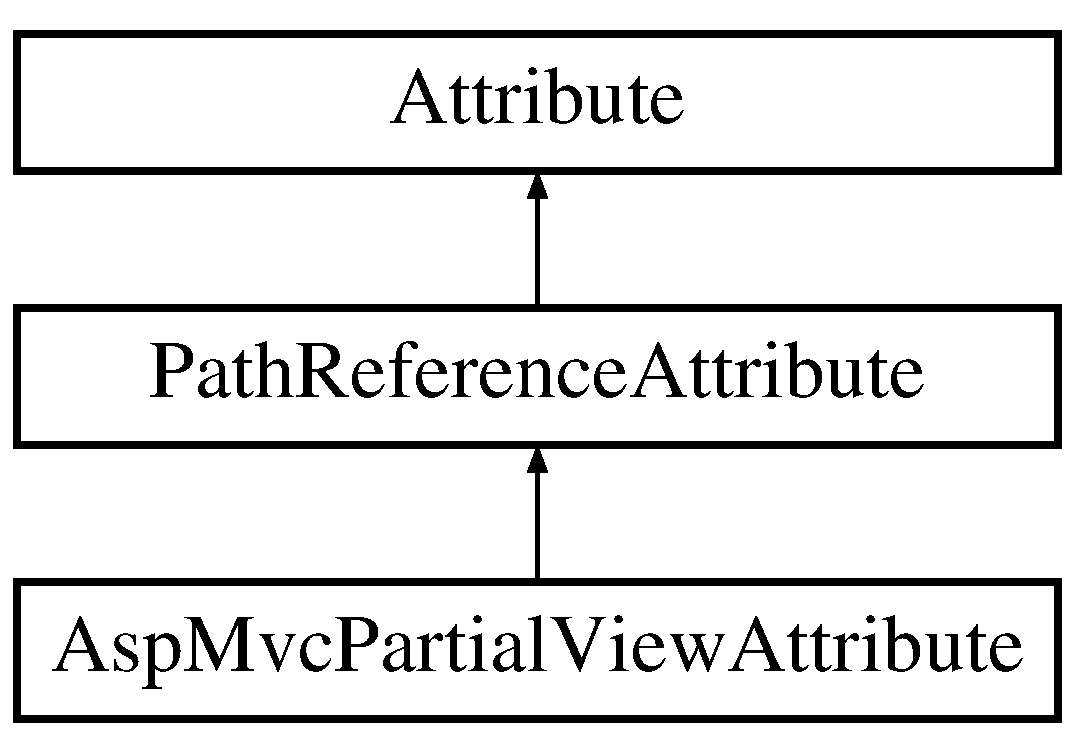
\includegraphics[height=3.000000cm]{class_asp_mvc_partial_view_attribute}
\end{center}
\end{figure}
\subsection*{Additional Inherited Members}


\subsection{Detailed Description}
A\+S\+P.\+N\+E\+T M\+V\+C attribute. If applied to a parameter, indicates that the parameter is an M\+V\+C partial view. If applied to a method, the M\+V\+C partial view name is calculated implicitly from the context. Use this attribute for custom wrappers similar to {\ttfamily System.\+Web.\+Mvc.\+Html.\+Render\+Partial\+Extensions.\+Render\+Partial(\+Html\+Helper, String)} 



The documentation for this class was generated from the following file\+:\begin{DoxyCompactItemize}
\item 
Documents/\+Git\+Hub/1-\/aarsproeve/1aarsproeve/1aarsproeve/\+Properties/Annotations.\+cs\end{DoxyCompactItemize}

\hypertarget{class_asp_mvc_partial_view_location_format_attribute}{}\section{Asp\+Mvc\+Partial\+View\+Location\+Format\+Attribute Class Reference}
\label{class_asp_mvc_partial_view_location_format_attribute}\index{Asp\+Mvc\+Partial\+View\+Location\+Format\+Attribute@{Asp\+Mvc\+Partial\+View\+Location\+Format\+Attribute}}
Inheritance diagram for Asp\+Mvc\+Partial\+View\+Location\+Format\+Attribute\+:\begin{figure}[H]
\begin{center}
\leavevmode
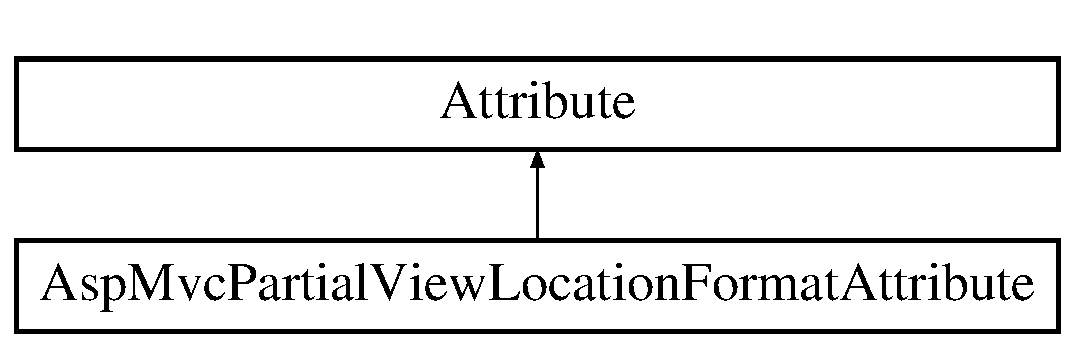
\includegraphics[height=2.000000cm]{class_asp_mvc_partial_view_location_format_attribute}
\end{center}
\end{figure}
\subsection*{Public Member Functions}
\begin{DoxyCompactItemize}
\item 
\hypertarget{class_asp_mvc_partial_view_location_format_attribute_a890db06863b6c2b93fbdb6435b512411}{}{\bfseries Asp\+Mvc\+Partial\+View\+Location\+Format\+Attribute} (string format)\label{class_asp_mvc_partial_view_location_format_attribute_a890db06863b6c2b93fbdb6435b512411}

\end{DoxyCompactItemize}
\subsection*{Properties}
\begin{DoxyCompactItemize}
\item 
\hypertarget{class_asp_mvc_partial_view_location_format_attribute_ab75cab80e0a441e206eadb7adce25efd}{}string {\bfseries Format}\hspace{0.3cm}{\ttfamily  \mbox{[}get\mbox{]}}\label{class_asp_mvc_partial_view_location_format_attribute_ab75cab80e0a441e206eadb7adce25efd}

\end{DoxyCompactItemize}


The documentation for this class was generated from the following file\+:\begin{DoxyCompactItemize}
\item 
Documents/\+Git\+Hub/1-\/aarsproeve/1aarsproeve/1aarsproeve/\+Properties/Annotations.\+cs\end{DoxyCompactItemize}

\hypertarget{class_asp_mvc_supress_view_error_attribute}{}\section{Asp\+Mvc\+Supress\+View\+Error\+Attribute Class Reference}
\label{class_asp_mvc_supress_view_error_attribute}\index{Asp\+Mvc\+Supress\+View\+Error\+Attribute@{Asp\+Mvc\+Supress\+View\+Error\+Attribute}}


A\+S\+P.\+N\+E\+T M\+V\+C attribute. Allows disabling inspections for M\+V\+C views within a class or a method  


Inheritance diagram for Asp\+Mvc\+Supress\+View\+Error\+Attribute\+:\begin{figure}[H]
\begin{center}
\leavevmode
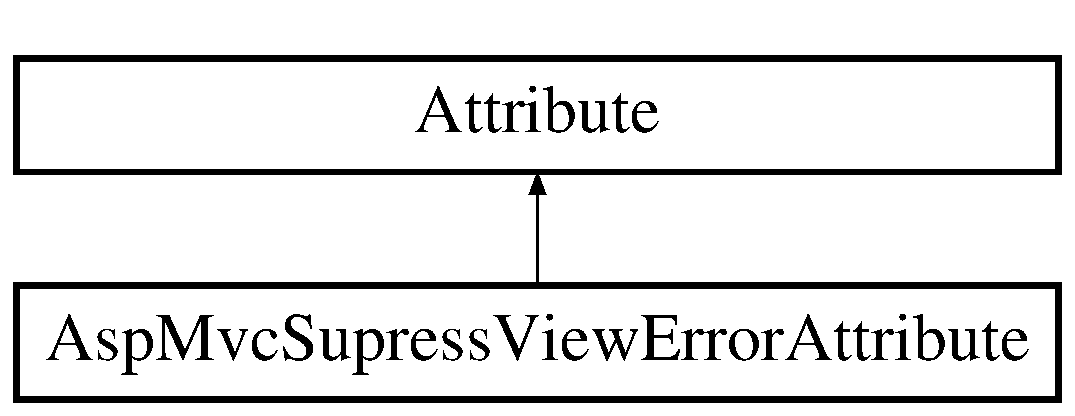
\includegraphics[height=2.000000cm]{class_asp_mvc_supress_view_error_attribute}
\end{center}
\end{figure}


\subsection{Detailed Description}
A\+S\+P.\+N\+E\+T M\+V\+C attribute. Allows disabling inspections for M\+V\+C views within a class or a method 



The documentation for this class was generated from the following file\+:\begin{DoxyCompactItemize}
\item 
Documents/\+Git\+Hub/1-\/aarsproeve/1aarsproeve/1aarsproeve/\+Properties/Annotations.\+cs\end{DoxyCompactItemize}

\hypertarget{class_asp_mvc_template_attribute}{}\section{Asp\+Mvc\+Template\+Attribute Class Reference}
\label{class_asp_mvc_template_attribute}\index{Asp\+Mvc\+Template\+Attribute@{Asp\+Mvc\+Template\+Attribute}}


A\+S\+P.\+N\+E\+T M\+V\+C attribute. Indicates that a parameter is an M\+V\+C template. Use this attribute for custom wrappers similar to {\ttfamily System.\+Component\+Model.\+Data\+Annotations.\+U\+I\+Hint\+Attribute(System.\+String)}  


Inheritance diagram for Asp\+Mvc\+Template\+Attribute\+:\begin{figure}[H]
\begin{center}
\leavevmode
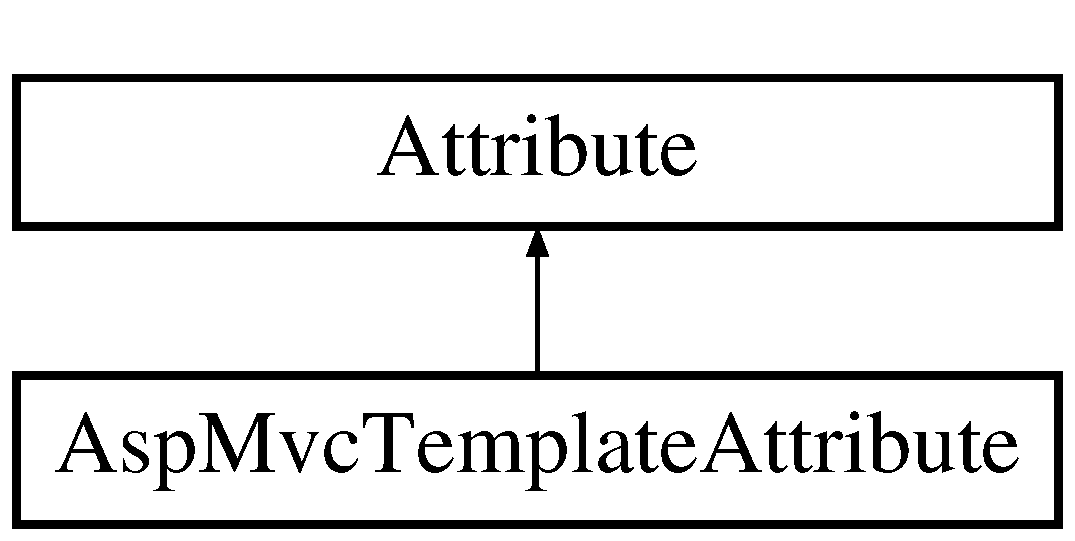
\includegraphics[height=2.000000cm]{class_asp_mvc_template_attribute}
\end{center}
\end{figure}


\subsection{Detailed Description}
A\+S\+P.\+N\+E\+T M\+V\+C attribute. Indicates that a parameter is an M\+V\+C template. Use this attribute for custom wrappers similar to {\ttfamily System.\+Component\+Model.\+Data\+Annotations.\+U\+I\+Hint\+Attribute(System.\+String)} 



The documentation for this class was generated from the following file\+:\begin{DoxyCompactItemize}
\item 
Documents/\+Git\+Hub/1-\/aarsproeve/1aarsproeve/1aarsproeve/\+Properties/Annotations.\+cs\end{DoxyCompactItemize}

\hypertarget{class_asp_mvc_view_attribute}{}\section{Asp\+Mvc\+View\+Attribute Class Reference}
\label{class_asp_mvc_view_attribute}\index{Asp\+Mvc\+View\+Attribute@{Asp\+Mvc\+View\+Attribute}}


A\+S\+P.\+N\+E\+T M\+V\+C attribute. If applied to a parameter, indicates that the parameter is an M\+V\+C view. If applied to a method, the M\+V\+C view name is calculated implicitly from the context. Use this attribute for custom wrappers similar to {\ttfamily System.\+Web.\+Mvc.\+Controller.\+View(\+Object)}  


Inheritance diagram for Asp\+Mvc\+View\+Attribute\+:\begin{figure}[H]
\begin{center}
\leavevmode
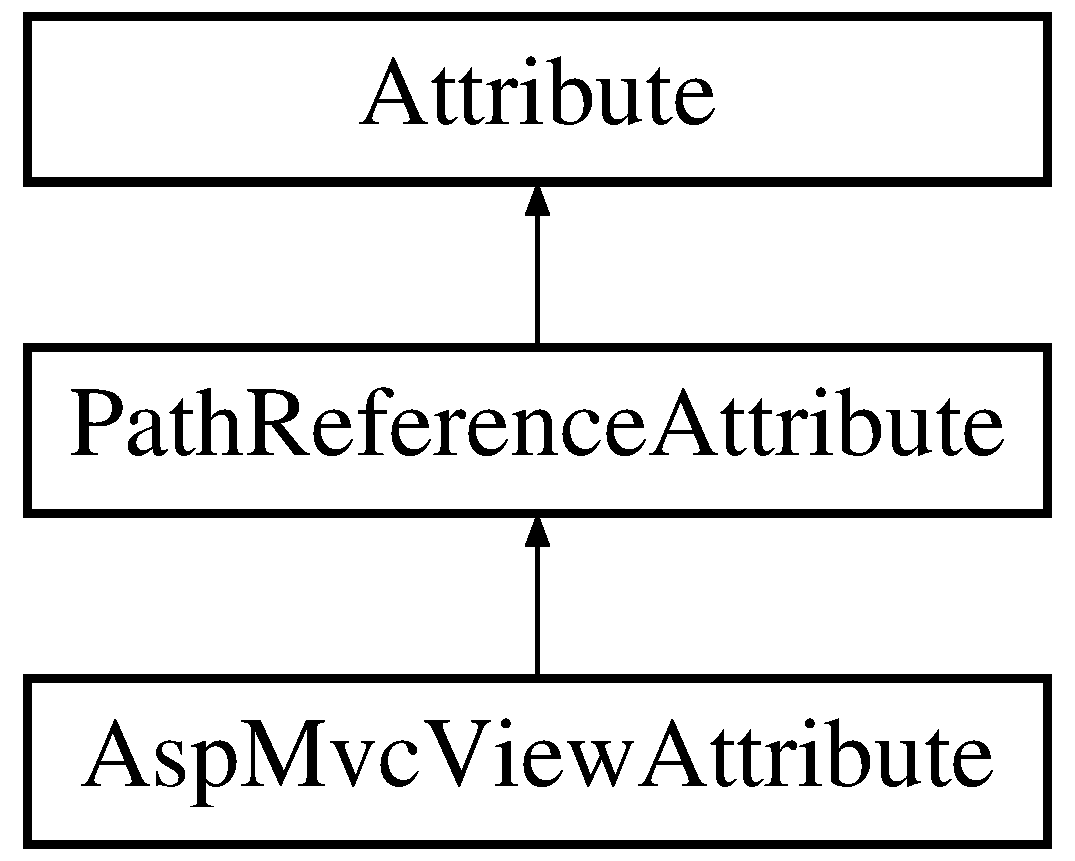
\includegraphics[height=3.000000cm]{class_asp_mvc_view_attribute}
\end{center}
\end{figure}
\subsection*{Additional Inherited Members}


\subsection{Detailed Description}
A\+S\+P.\+N\+E\+T M\+V\+C attribute. If applied to a parameter, indicates that the parameter is an M\+V\+C view. If applied to a method, the M\+V\+C view name is calculated implicitly from the context. Use this attribute for custom wrappers similar to {\ttfamily System.\+Web.\+Mvc.\+Controller.\+View(\+Object)} 



The documentation for this class was generated from the following file\+:\begin{DoxyCompactItemize}
\item 
Documents/\+Git\+Hub/1-\/aarsproeve/1aarsproeve/1aarsproeve/\+Properties/Annotations.\+cs\end{DoxyCompactItemize}

\hypertarget{class_asp_mvc_view_location_format_attribute}{}\section{Asp\+Mvc\+View\+Location\+Format\+Attribute Class Reference}
\label{class_asp_mvc_view_location_format_attribute}\index{Asp\+Mvc\+View\+Location\+Format\+Attribute@{Asp\+Mvc\+View\+Location\+Format\+Attribute}}
Inheritance diagram for Asp\+Mvc\+View\+Location\+Format\+Attribute\+:\begin{figure}[H]
\begin{center}
\leavevmode
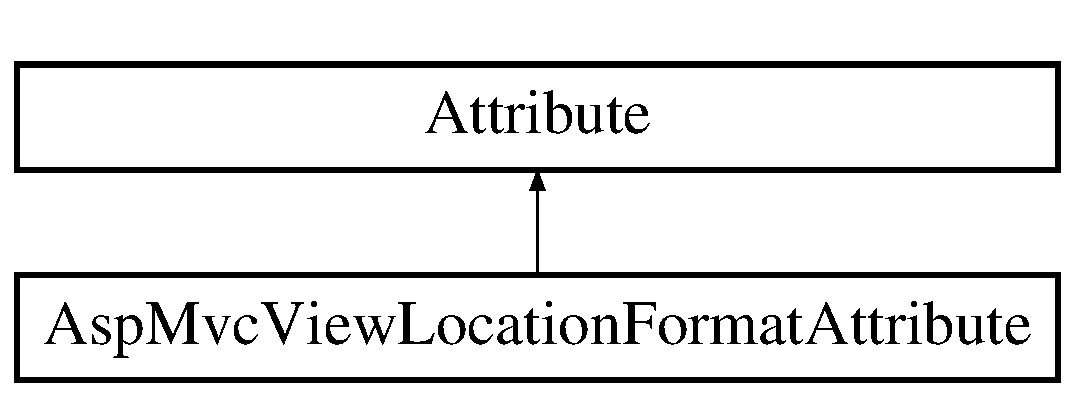
\includegraphics[height=2.000000cm]{class_asp_mvc_view_location_format_attribute}
\end{center}
\end{figure}
\subsection*{Public Member Functions}
\begin{DoxyCompactItemize}
\item 
\hypertarget{class_asp_mvc_view_location_format_attribute_aecb3c29d8605da500d4af960ba99f207}{}{\bfseries Asp\+Mvc\+View\+Location\+Format\+Attribute} (string format)\label{class_asp_mvc_view_location_format_attribute_aecb3c29d8605da500d4af960ba99f207}

\end{DoxyCompactItemize}
\subsection*{Properties}
\begin{DoxyCompactItemize}
\item 
\hypertarget{class_asp_mvc_view_location_format_attribute_a3489b3971df02310fd8abb286247c4ae}{}string {\bfseries Format}\hspace{0.3cm}{\ttfamily  \mbox{[}get\mbox{]}}\label{class_asp_mvc_view_location_format_attribute_a3489b3971df02310fd8abb286247c4ae}

\end{DoxyCompactItemize}


The documentation for this class was generated from the following file\+:\begin{DoxyCompactItemize}
\item 
Documents/\+Git\+Hub/1-\/aarsproeve/1aarsproeve/1aarsproeve/\+Properties/Annotations.\+cs\end{DoxyCompactItemize}

\hypertarget{class_asp_required_attribute_attribute}{}\section{Asp\+Required\+Attribute\+Attribute Class Reference}
\label{class_asp_required_attribute_attribute}\index{Asp\+Required\+Attribute\+Attribute@{Asp\+Required\+Attribute\+Attribute}}
Inheritance diagram for Asp\+Required\+Attribute\+Attribute\+:\begin{figure}[H]
\begin{center}
\leavevmode
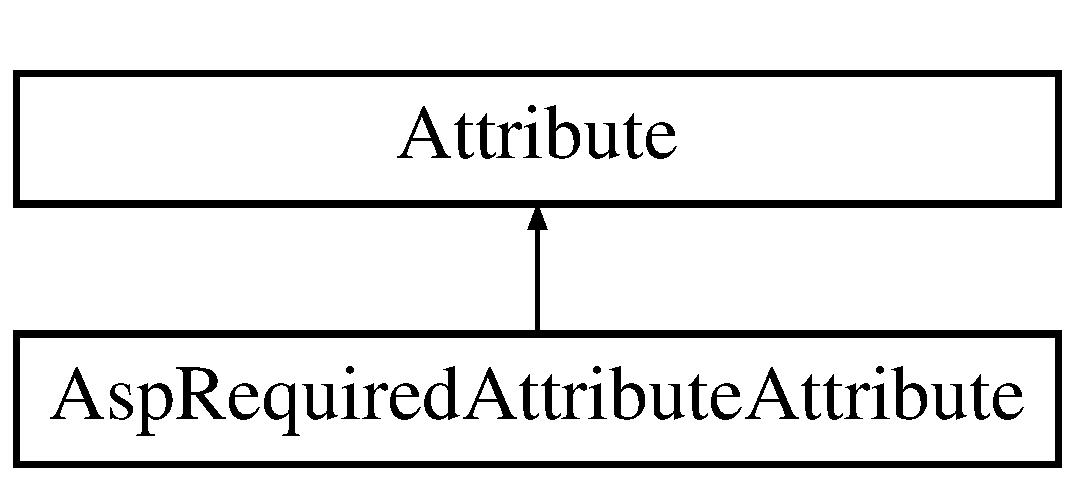
\includegraphics[height=2.000000cm]{class_asp_required_attribute_attribute}
\end{center}
\end{figure}
\subsection*{Public Member Functions}
\begin{DoxyCompactItemize}
\item 
\hypertarget{class_asp_required_attribute_attribute_a37e197f5a5990c0140d0dc75be9ad6a6}{}{\bfseries Asp\+Required\+Attribute\+Attribute} (\mbox{[}Not\+Null\mbox{]} string attribute)\label{class_asp_required_attribute_attribute_a37e197f5a5990c0140d0dc75be9ad6a6}

\end{DoxyCompactItemize}
\subsection*{Properties}
\begin{DoxyCompactItemize}
\item 
\hypertarget{class_asp_required_attribute_attribute_a8d782b24a958ba36ee4d63265a5db96d}{}string {\bfseries Attribute}\hspace{0.3cm}{\ttfamily  \mbox{[}get\mbox{]}}\label{class_asp_required_attribute_attribute_a8d782b24a958ba36ee4d63265a5db96d}

\end{DoxyCompactItemize}


The documentation for this class was generated from the following file\+:\begin{DoxyCompactItemize}
\item 
Documents/\+Git\+Hub/1-\/aarsproeve/1aarsproeve/1aarsproeve/\+Properties/Annotations.\+cs\end{DoxyCompactItemize}

\hypertarget{class_asp_type_property_attribute}{}\section{Asp\+Type\+Property\+Attribute Class Reference}
\label{class_asp_type_property_attribute}\index{Asp\+Type\+Property\+Attribute@{Asp\+Type\+Property\+Attribute}}
Inheritance diagram for Asp\+Type\+Property\+Attribute\+:\begin{figure}[H]
\begin{center}
\leavevmode
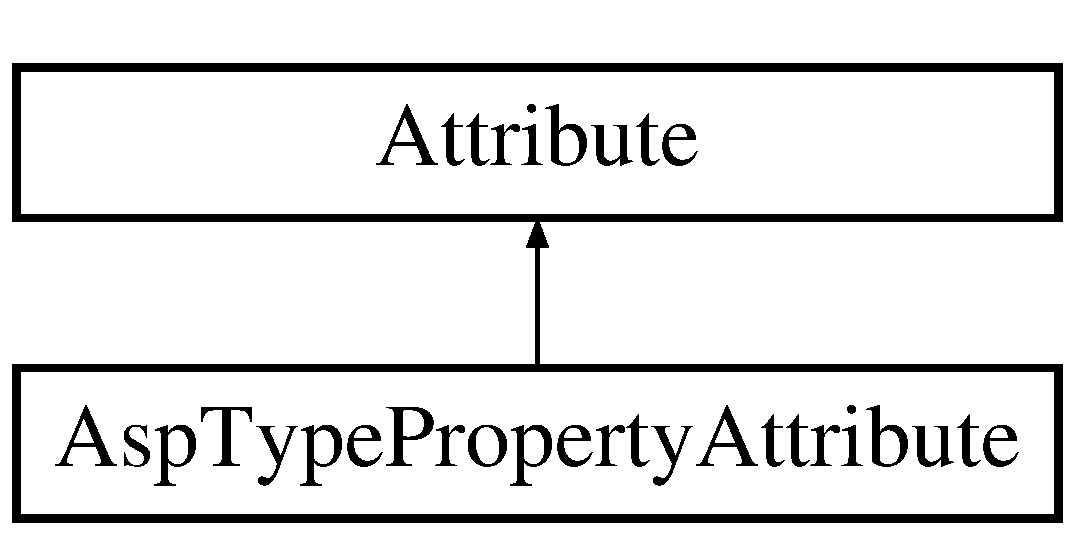
\includegraphics[height=2.000000cm]{class_asp_type_property_attribute}
\end{center}
\end{figure}
\subsection*{Public Member Functions}
\begin{DoxyCompactItemize}
\item 
\hypertarget{class_asp_type_property_attribute_a44e918652832a5c2272af6b3c85d12d1}{}{\bfseries Asp\+Type\+Property\+Attribute} (bool create\+Constructor\+References)\label{class_asp_type_property_attribute_a44e918652832a5c2272af6b3c85d12d1}

\end{DoxyCompactItemize}
\subsection*{Properties}
\begin{DoxyCompactItemize}
\item 
\hypertarget{class_asp_type_property_attribute_a57bbcf991d77058648e6292b63726241}{}bool {\bfseries Create\+Constructor\+References}\hspace{0.3cm}{\ttfamily  \mbox{[}get\mbox{]}}\label{class_asp_type_property_attribute_a57bbcf991d77058648e6292b63726241}

\end{DoxyCompactItemize}


The documentation for this class was generated from the following file\+:\begin{DoxyCompactItemize}
\item 
Documents/\+Git\+Hub/1-\/aarsproeve/1aarsproeve/1aarsproeve/\+Properties/Annotations.\+cs\end{DoxyCompactItemize}

\hypertarget{class_assertion_condition_attribute}{}\section{Assertion\+Condition\+Attribute Class Reference}
\label{class_assertion_condition_attribute}\index{Assertion\+Condition\+Attribute@{Assertion\+Condition\+Attribute}}


Indicates the condition parameter of the assertion method. The method itself should be marked by \hyperlink{class_assertion_method_attribute}{Assertion\+Method\+Attribute} attribute. The mandatory argument of the attribute is the assertion type.  


Inheritance diagram for Assertion\+Condition\+Attribute\+:\begin{figure}[H]
\begin{center}
\leavevmode
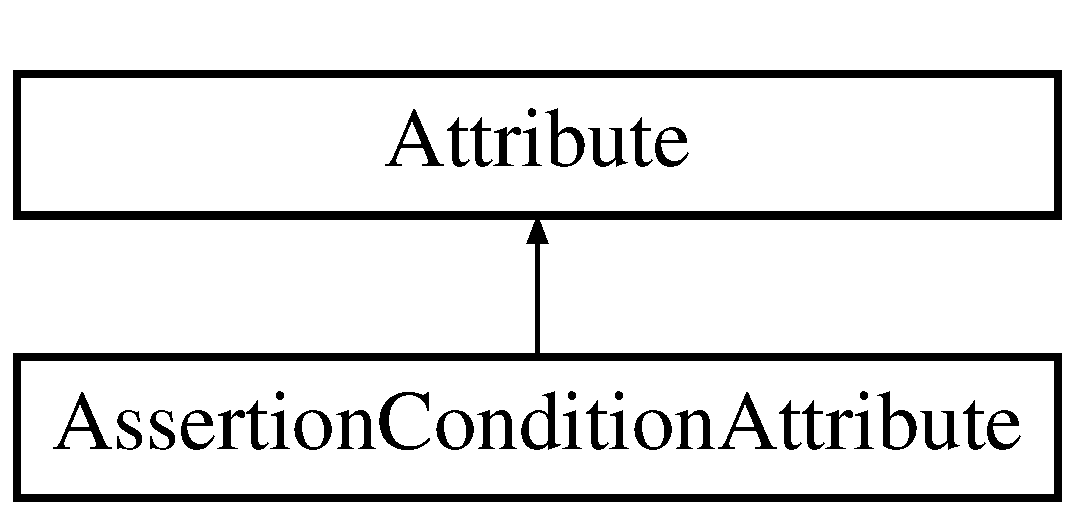
\includegraphics[height=2.000000cm]{class_assertion_condition_attribute}
\end{center}
\end{figure}
\subsection*{Public Member Functions}
\begin{DoxyCompactItemize}
\item 
\hypertarget{class_assertion_condition_attribute_a9e8e78b2fe91bb29f18154940860af32}{}{\bfseries Assertion\+Condition\+Attribute} (Assertion\+Condition\+Type condition\+Type)\label{class_assertion_condition_attribute_a9e8e78b2fe91bb29f18154940860af32}

\end{DoxyCompactItemize}
\subsection*{Properties}
\begin{DoxyCompactItemize}
\item 
\hypertarget{class_assertion_condition_attribute_ad07b5dd15df52a5c307ed41dda8299ef}{}Assertion\+Condition\+Type {\bfseries Condition\+Type}\hspace{0.3cm}{\ttfamily  \mbox{[}get\mbox{]}}\label{class_assertion_condition_attribute_ad07b5dd15df52a5c307ed41dda8299ef}

\end{DoxyCompactItemize}


\subsection{Detailed Description}
Indicates the condition parameter of the assertion method. The method itself should be marked by \hyperlink{class_assertion_method_attribute}{Assertion\+Method\+Attribute} attribute. The mandatory argument of the attribute is the assertion type. 



The documentation for this class was generated from the following file\+:\begin{DoxyCompactItemize}
\item 
Documents/\+Git\+Hub/1-\/aarsproeve/1aarsproeve/1aarsproeve/\+Properties/Annotations.\+cs\end{DoxyCompactItemize}

\hypertarget{class_assertion_method_attribute}{}\section{Assertion\+Method\+Attribute Class Reference}
\label{class_assertion_method_attribute}\index{Assertion\+Method\+Attribute@{Assertion\+Method\+Attribute}}


Indicates that the marked method is assertion method, i.\+e. it halts control flow if one of the conditions is satisfied. To set the condition, mark one of the parameters with \hyperlink{class_assertion_condition_attribute}{Assertion\+Condition\+Attribute} attribute  


Inheritance diagram for Assertion\+Method\+Attribute\+:\begin{figure}[H]
\begin{center}
\leavevmode
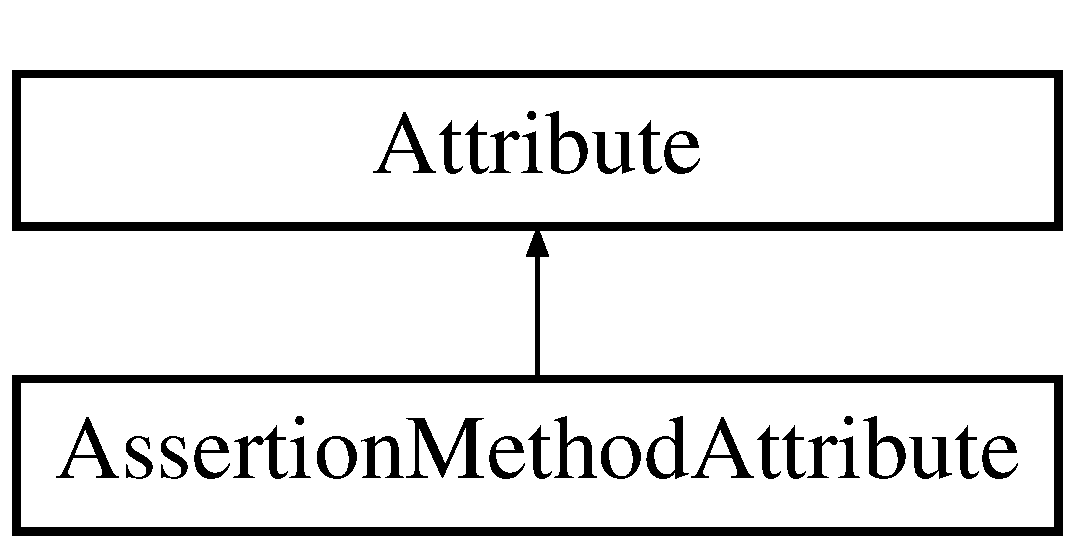
\includegraphics[height=2.000000cm]{class_assertion_method_attribute}
\end{center}
\end{figure}


\subsection{Detailed Description}
Indicates that the marked method is assertion method, i.\+e. it halts control flow if one of the conditions is satisfied. To set the condition, mark one of the parameters with \hyperlink{class_assertion_condition_attribute}{Assertion\+Condition\+Attribute} attribute 



The documentation for this class was generated from the following file\+:\begin{DoxyCompactItemize}
\item 
Documents/\+Git\+Hub/1-\/aarsproeve/1aarsproeve/1aarsproeve/\+Properties/Annotations.\+cs\end{DoxyCompactItemize}

\hypertarget{class_base_type_required_attribute}{}\section{Base\+Type\+Required\+Attribute Class Reference}
\label{class_base_type_required_attribute}\index{Base\+Type\+Required\+Attribute@{Base\+Type\+Required\+Attribute}}


When applied to a target attribute, specifies a requirement for any type marked with the target attribute to implement or inherit specific type or types.  


Inheritance diagram for Base\+Type\+Required\+Attribute\+:\begin{figure}[H]
\begin{center}
\leavevmode
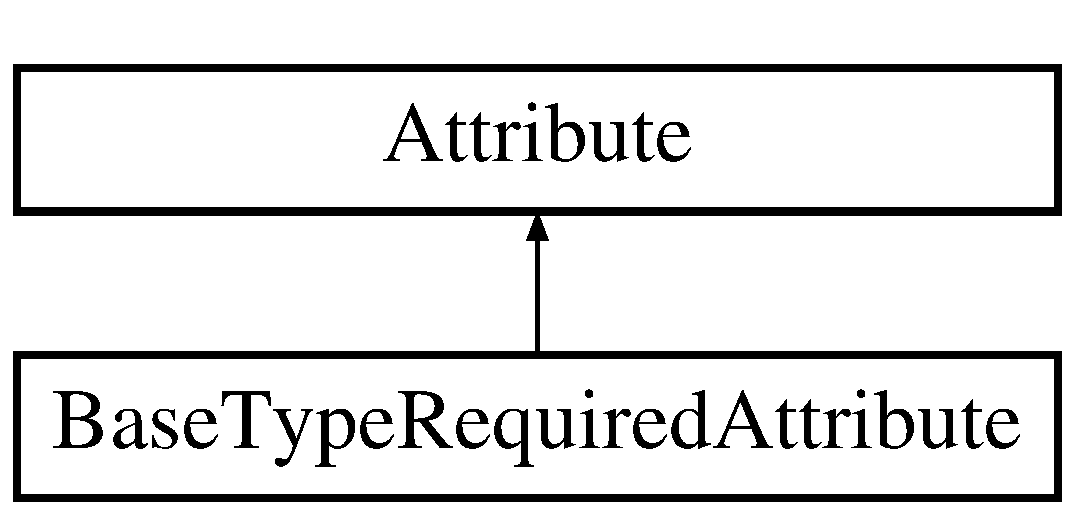
\includegraphics[height=2.000000cm]{class_base_type_required_attribute}
\end{center}
\end{figure}
\subsection*{Public Member Functions}
\begin{DoxyCompactItemize}
\item 
\hypertarget{class_base_type_required_attribute_a3b535405fd33291328613b6ede4e5d8a}{}{\bfseries Base\+Type\+Required\+Attribute} (\mbox{[}Not\+Null\mbox{]} Type base\+Type)\label{class_base_type_required_attribute_a3b535405fd33291328613b6ede4e5d8a}

\end{DoxyCompactItemize}
\subsection*{Properties}
\begin{DoxyCompactItemize}
\item 
\hypertarget{class_base_type_required_attribute_abd32451b36cd8eff34ecee4718e78f5b}{}Type {\bfseries Base\+Type}\hspace{0.3cm}{\ttfamily  \mbox{[}get\mbox{]}}\label{class_base_type_required_attribute_abd32451b36cd8eff34ecee4718e78f5b}

\end{DoxyCompactItemize}


\subsection{Detailed Description}
When applied to a target attribute, specifies a requirement for any type marked with the target attribute to implement or inherit specific type or types. 


\begin{DoxyCode}
[BaseTypeRequired(typeof(IComponent)] \textcolor{comment}{// Specify requirement}
\textcolor{keyword}{public} \textcolor{keyword}{class} ComponentAttribute : Attribute \{ \}
[Component] \textcolor{comment}{// ComponentAttribute requires implementing IComponent interface}
\textcolor{keyword}{public} \textcolor{keyword}{class }MyComponent : IComponent \{ \}
\end{DoxyCode}


The documentation for this class was generated from the following file\+:\begin{DoxyCompactItemize}
\item 
Documents/\+Git\+Hub/1-\/aarsproeve/1aarsproeve/1aarsproeve/\+Properties/Annotations.\+cs\end{DoxyCompactItemize}

\hypertarget{class__1aarsproeve_web_service_1_1_beskeder}{}\section{\+\_\+1aarsproeve\+Web\+Service.\+Beskeder Class Reference}
\label{class__1aarsproeve_web_service_1_1_beskeder}\index{\+\_\+1aarsproeve\+Web\+Service.\+Beskeder@{\+\_\+1aarsproeve\+Web\+Service.\+Beskeder}}
\subsection*{Properties}
\begin{DoxyCompactItemize}
\item 
\hypertarget{class__1aarsproeve_web_service_1_1_beskeder_ac09e7a6d3196777938c99fcdc259fdb4}{}int {\bfseries Besked\+Id}\hspace{0.3cm}{\ttfamily  \mbox{[}get, set\mbox{]}}\label{class__1aarsproeve_web_service_1_1_beskeder_ac09e7a6d3196777938c99fcdc259fdb4}

\item 
\hypertarget{class__1aarsproeve_web_service_1_1_beskeder_a864f1489fab328277d4a03a3416ad3f9}{}string {\bfseries Overskrift}\hspace{0.3cm}{\ttfamily  \mbox{[}get, set\mbox{]}}\label{class__1aarsproeve_web_service_1_1_beskeder_a864f1489fab328277d4a03a3416ad3f9}

\item 
\hypertarget{class__1aarsproeve_web_service_1_1_beskeder_abb534e75d449df7de7da2af259a7d52b}{}Date\+Time {\bfseries Dato}\hspace{0.3cm}{\ttfamily  \mbox{[}get, set\mbox{]}}\label{class__1aarsproeve_web_service_1_1_beskeder_abb534e75d449df7de7da2af259a7d52b}

\item 
\hypertarget{class__1aarsproeve_web_service_1_1_beskeder_a7ff25701d9b4ca4e372cd0c9620dd7bc}{}string {\bfseries Beskrivelse}\hspace{0.3cm}{\ttfamily  \mbox{[}get, set\mbox{]}}\label{class__1aarsproeve_web_service_1_1_beskeder_a7ff25701d9b4ca4e372cd0c9620dd7bc}

\item 
\hypertarget{class__1aarsproeve_web_service_1_1_beskeder_a5fa573e7bbf0fd8acd75c52a6f29d796}{}Date\+Time {\bfseries Udloebsdato}\hspace{0.3cm}{\ttfamily  \mbox{[}get, set\mbox{]}}\label{class__1aarsproeve_web_service_1_1_beskeder_a5fa573e7bbf0fd8acd75c52a6f29d796}

\item 
\hypertarget{class__1aarsproeve_web_service_1_1_beskeder_a8e9e54630b3514f3ed5c89ce153df96c}{}string {\bfseries Brugernavn}\hspace{0.3cm}{\ttfamily  \mbox{[}get, set\mbox{]}}\label{class__1aarsproeve_web_service_1_1_beskeder_a8e9e54630b3514f3ed5c89ce153df96c}

\item 
\hypertarget{class__1aarsproeve_web_service_1_1_beskeder_aa8074ce4b250925fe0635463000cacbd}{}virtual \hyperlink{class__1aarsproeve_web_service_1_1_ansatte}{Ansatte} {\bfseries Ansatte}\hspace{0.3cm}{\ttfamily  \mbox{[}get, set\mbox{]}}\label{class__1aarsproeve_web_service_1_1_beskeder_aa8074ce4b250925fe0635463000cacbd}

\end{DoxyCompactItemize}


The documentation for this class was generated from the following file\+:\begin{DoxyCompactItemize}
\item 
Documents/\+Git\+Hub/1-\/aarsproeve/1aarsproeve/1aarsproeve\+Web\+Service/Beskeder.\+cs\end{DoxyCompactItemize}

\hypertarget{class_w_s1aarsproeve_1_1_beskeder}{}\section{W\+S1aarsproeve.\+Beskeder Class Reference}
\label{class_w_s1aarsproeve_1_1_beskeder}\index{W\+S1aarsproeve.\+Beskeder@{W\+S1aarsproeve.\+Beskeder}}
\subsection*{Properties}
\begin{DoxyCompactItemize}
\item 
\hypertarget{class_w_s1aarsproeve_1_1_beskeder_afb5d4d4890212acdd20b9a9144acb8c9}{}int {\bfseries Besked\+Id}\hspace{0.3cm}{\ttfamily  \mbox{[}get, set\mbox{]}}\label{class_w_s1aarsproeve_1_1_beskeder_afb5d4d4890212acdd20b9a9144acb8c9}

\item 
\hypertarget{class_w_s1aarsproeve_1_1_beskeder_a26ab07ec2aa00e799717e7107da39ac3}{}string {\bfseries Overskrift}\hspace{0.3cm}{\ttfamily  \mbox{[}get, set\mbox{]}}\label{class_w_s1aarsproeve_1_1_beskeder_a26ab07ec2aa00e799717e7107da39ac3}

\item 
\hypertarget{class_w_s1aarsproeve_1_1_beskeder_a77960affa3d607c79ad2d36416e82990}{}Date\+Time {\bfseries Dato}\hspace{0.3cm}{\ttfamily  \mbox{[}get, set\mbox{]}}\label{class_w_s1aarsproeve_1_1_beskeder_a77960affa3d607c79ad2d36416e82990}

\item 
\hypertarget{class_w_s1aarsproeve_1_1_beskeder_a30ad86441d04c5d0c5e1a605c61d6d06}{}string {\bfseries Beskrivelse}\hspace{0.3cm}{\ttfamily  \mbox{[}get, set\mbox{]}}\label{class_w_s1aarsproeve_1_1_beskeder_a30ad86441d04c5d0c5e1a605c61d6d06}

\item 
\hypertarget{class_w_s1aarsproeve_1_1_beskeder_a9f84b7510fee3032f3649e9aa6283e48}{}Date\+Time {\bfseries Udloebsdato}\hspace{0.3cm}{\ttfamily  \mbox{[}get, set\mbox{]}}\label{class_w_s1aarsproeve_1_1_beskeder_a9f84b7510fee3032f3649e9aa6283e48}

\item 
\hypertarget{class_w_s1aarsproeve_1_1_beskeder_ac062915cd5f28e2122bce255b63e7e74}{}string {\bfseries Brugernavn}\hspace{0.3cm}{\ttfamily  \mbox{[}get, set\mbox{]}}\label{class_w_s1aarsproeve_1_1_beskeder_ac062915cd5f28e2122bce255b63e7e74}

\item 
\hypertarget{class_w_s1aarsproeve_1_1_beskeder_ad5f19abc95df1b1b1a015a5850a4e3d9}{}virtual \hyperlink{class_w_s1aarsproeve_1_1_ansatte}{Ansatte} {\bfseries Ansatte}\hspace{0.3cm}{\ttfamily  \mbox{[}get, set\mbox{]}}\label{class_w_s1aarsproeve_1_1_beskeder_ad5f19abc95df1b1b1a015a5850a4e3d9}

\end{DoxyCompactItemize}


The documentation for this class was generated from the following file\+:\begin{DoxyCompactItemize}
\item 
Documents/\+Git\+Hub/1-\/aarsproeve/1aarsproeve/\+W\+S1aarsproeve/\+Models/Beskeder.\+cs\end{DoxyCompactItemize}

\hypertarget{class__1aarsproeve_1_1_model_1_1_beskeder}{}\section{\+\_\+1aarsproeve.\+Model.\+Beskeder Class Reference}
\label{class__1aarsproeve_1_1_model_1_1_beskeder}\index{\+\_\+1aarsproeve.\+Model.\+Beskeder@{\+\_\+1aarsproeve.\+Model.\+Beskeder}}


Besked klasse der holder styr p� f�llesbeskeder  


\subsection*{Public Member Functions}
\begin{DoxyCompactItemize}
\item 
\hyperlink{class__1aarsproeve_1_1_model_1_1_beskeder_a5790eafeeb8c1805cc9d4ed27c7fee90}{Beskeder} (int besked\+Id, string overskrift, Date\+Time dato, string beskrivelse, Date\+Time udloebsdato, string brugernavn)
\begin{DoxyCompactList}\small\item\em Konstrukt�r til \hyperlink{class__1aarsproeve_1_1_model_1_1_beskeder}{Beskeder} klassen \end{DoxyCompactList}\item 
\hyperlink{class__1aarsproeve_1_1_model_1_1_beskeder_a3cdb3070a8fd22fe45a75e1e62cd9387}{Beskeder} ()
\begin{DoxyCompactList}\small\item\em Default konstrukt�r \end{DoxyCompactList}\item 
\hypertarget{class__1aarsproeve_1_1_model_1_1_beskeder_ae1ecf7e093ab61b194b55560f123f80b}{}void {\bfseries Check\+Beskrivelse} (string beskrivelse)\label{class__1aarsproeve_1_1_model_1_1_beskeder_ae1ecf7e093ab61b194b55560f123f80b}

\item 
\hypertarget{class__1aarsproeve_1_1_model_1_1_beskeder_a50d923f637746874880b6fb2feac84c2}{}void {\bfseries Check\+Brugernavn} (string brugernavn)\label{class__1aarsproeve_1_1_model_1_1_beskeder_a50d923f637746874880b6fb2feac84c2}

\item 
\hypertarget{class__1aarsproeve_1_1_model_1_1_beskeder_a99904c0bab4e30d45989cb38882812f6}{}void {\bfseries Check\+Overskrift} (string overskrift)\label{class__1aarsproeve_1_1_model_1_1_beskeder_a99904c0bab4e30d45989cb38882812f6}

\end{DoxyCompactItemize}
\subsection*{Properties}
\begin{DoxyCompactItemize}
\item 
int \hyperlink{class__1aarsproeve_1_1_model_1_1_beskeder_a81b913e9bc51d39069b98df772bad312}{Besked\+Id}\hspace{0.3cm}{\ttfamily  \mbox{[}get, set\mbox{]}}
\begin{DoxyCompactList}\small\item\em Besked\+Id Property \end{DoxyCompactList}\item 
string \hyperlink{class__1aarsproeve_1_1_model_1_1_beskeder_aaca56c9b07a75deee580a47f950afb88}{Overskrift}\hspace{0.3cm}{\ttfamily  \mbox{[}get, set\mbox{]}}
\begin{DoxyCompactList}\small\item\em Overskrift Property \end{DoxyCompactList}\item 
Date\+Time \hyperlink{class__1aarsproeve_1_1_model_1_1_beskeder_a5f459d40a91e821c9f58924a1316e86a}{Dato}\hspace{0.3cm}{\ttfamily  \mbox{[}get, set\mbox{]}}
\begin{DoxyCompactList}\small\item\em Dato Property \end{DoxyCompactList}\item 
string \hyperlink{class__1aarsproeve_1_1_model_1_1_beskeder_a0145d64de806cf78039ff6c50116105b}{Beskrivelse}\hspace{0.3cm}{\ttfamily  \mbox{[}get, set\mbox{]}}
\begin{DoxyCompactList}\small\item\em Beskrivelse Property \end{DoxyCompactList}\item 
Date\+Time \hyperlink{class__1aarsproeve_1_1_model_1_1_beskeder_a332cfb48d7aab3f0bc291d1cb426a494}{Udloebsdato}\hspace{0.3cm}{\ttfamily  \mbox{[}get, set\mbox{]}}
\begin{DoxyCompactList}\small\item\em Udloebsdato Property \end{DoxyCompactList}\item 
string \hyperlink{class__1aarsproeve_1_1_model_1_1_beskeder_a3f225b075a4f64832b33e0d1e61b0f4e}{Brugernavn}\hspace{0.3cm}{\ttfamily  \mbox{[}get, set\mbox{]}}
\begin{DoxyCompactList}\small\item\em Brugernavn Property \end{DoxyCompactList}\end{DoxyCompactItemize}


\subsection{Detailed Description}
Besked klasse der holder styr p� f�llesbeskeder 



\subsection{Constructor \& Destructor Documentation}
\hypertarget{class__1aarsproeve_1_1_model_1_1_beskeder_a5790eafeeb8c1805cc9d4ed27c7fee90}{}\index{\+\_\+1aarsproeve\+::\+Model\+::\+Beskeder@{\+\_\+1aarsproeve\+::\+Model\+::\+Beskeder}!Beskeder@{Beskeder}}
\index{Beskeder@{Beskeder}!\+\_\+1aarsproeve\+::\+Model\+::\+Beskeder@{\+\_\+1aarsproeve\+::\+Model\+::\+Beskeder}}
\subsubsection[{Beskeder}]{\setlength{\rightskip}{0pt plus 5cm}\+\_\+1aarsproeve.\+Model.\+Beskeder.\+Beskeder (
\begin{DoxyParamCaption}
\item[{int}]{besked\+Id, }
\item[{string}]{overskrift, }
\item[{Date\+Time}]{dato, }
\item[{string}]{beskrivelse, }
\item[{Date\+Time}]{udloebsdato, }
\item[{string}]{brugernavn}
\end{DoxyParamCaption}
)}\label{class__1aarsproeve_1_1_model_1_1_beskeder_a5790eafeeb8c1805cc9d4ed27c7fee90}


Konstrukt�r til \hyperlink{class__1aarsproeve_1_1_model_1_1_beskeder}{Beskeder} klassen 


\begin{DoxyParams}{Parameters}
{\em besked\+Id} & besked\+Id parameter\\
\hline
{\em overskrift} & overskrift parameter\\
\hline
{\em dato} & dato parameter\\
\hline
{\em beskrivelse} & beskrivelse parameter\\
\hline
{\em udloebsdato} & udloebsdato parameter\\
\hline
{\em brugernavn} & brugernavn parameter\\
\hline
\end{DoxyParams}
\hypertarget{class__1aarsproeve_1_1_model_1_1_beskeder_a3cdb3070a8fd22fe45a75e1e62cd9387}{}\index{\+\_\+1aarsproeve\+::\+Model\+::\+Beskeder@{\+\_\+1aarsproeve\+::\+Model\+::\+Beskeder}!Beskeder@{Beskeder}}
\index{Beskeder@{Beskeder}!\+\_\+1aarsproeve\+::\+Model\+::\+Beskeder@{\+\_\+1aarsproeve\+::\+Model\+::\+Beskeder}}
\subsubsection[{Beskeder}]{\setlength{\rightskip}{0pt plus 5cm}\+\_\+1aarsproeve.\+Model.\+Beskeder.\+Beskeder (
\begin{DoxyParamCaption}
{}
\end{DoxyParamCaption}
)}\label{class__1aarsproeve_1_1_model_1_1_beskeder_a3cdb3070a8fd22fe45a75e1e62cd9387}


Default konstrukt�r 



\subsection{Property Documentation}
\hypertarget{class__1aarsproeve_1_1_model_1_1_beskeder_a81b913e9bc51d39069b98df772bad312}{}\index{\+\_\+1aarsproeve\+::\+Model\+::\+Beskeder@{\+\_\+1aarsproeve\+::\+Model\+::\+Beskeder}!Besked\+Id@{Besked\+Id}}
\index{Besked\+Id@{Besked\+Id}!\+\_\+1aarsproeve\+::\+Model\+::\+Beskeder@{\+\_\+1aarsproeve\+::\+Model\+::\+Beskeder}}
\subsubsection[{Besked\+Id}]{\setlength{\rightskip}{0pt plus 5cm}int \+\_\+1aarsproeve.\+Model.\+Beskeder.\+Besked\+Id\hspace{0.3cm}{\ttfamily [get]}, {\ttfamily [set]}}\label{class__1aarsproeve_1_1_model_1_1_beskeder_a81b913e9bc51d39069b98df772bad312}


Besked\+Id Property 

\hypertarget{class__1aarsproeve_1_1_model_1_1_beskeder_a0145d64de806cf78039ff6c50116105b}{}\index{\+\_\+1aarsproeve\+::\+Model\+::\+Beskeder@{\+\_\+1aarsproeve\+::\+Model\+::\+Beskeder}!Beskrivelse@{Beskrivelse}}
\index{Beskrivelse@{Beskrivelse}!\+\_\+1aarsproeve\+::\+Model\+::\+Beskeder@{\+\_\+1aarsproeve\+::\+Model\+::\+Beskeder}}
\subsubsection[{Beskrivelse}]{\setlength{\rightskip}{0pt plus 5cm}string \+\_\+1aarsproeve.\+Model.\+Beskeder.\+Beskrivelse\hspace{0.3cm}{\ttfamily [get]}, {\ttfamily [set]}}\label{class__1aarsproeve_1_1_model_1_1_beskeder_a0145d64de806cf78039ff6c50116105b}


Beskrivelse Property 

\hypertarget{class__1aarsproeve_1_1_model_1_1_beskeder_a3f225b075a4f64832b33e0d1e61b0f4e}{}\index{\+\_\+1aarsproeve\+::\+Model\+::\+Beskeder@{\+\_\+1aarsproeve\+::\+Model\+::\+Beskeder}!Brugernavn@{Brugernavn}}
\index{Brugernavn@{Brugernavn}!\+\_\+1aarsproeve\+::\+Model\+::\+Beskeder@{\+\_\+1aarsproeve\+::\+Model\+::\+Beskeder}}
\subsubsection[{Brugernavn}]{\setlength{\rightskip}{0pt plus 5cm}string \+\_\+1aarsproeve.\+Model.\+Beskeder.\+Brugernavn\hspace{0.3cm}{\ttfamily [get]}, {\ttfamily [set]}}\label{class__1aarsproeve_1_1_model_1_1_beskeder_a3f225b075a4f64832b33e0d1e61b0f4e}


Brugernavn Property 

\hypertarget{class__1aarsproeve_1_1_model_1_1_beskeder_a5f459d40a91e821c9f58924a1316e86a}{}\index{\+\_\+1aarsproeve\+::\+Model\+::\+Beskeder@{\+\_\+1aarsproeve\+::\+Model\+::\+Beskeder}!Dato@{Dato}}
\index{Dato@{Dato}!\+\_\+1aarsproeve\+::\+Model\+::\+Beskeder@{\+\_\+1aarsproeve\+::\+Model\+::\+Beskeder}}
\subsubsection[{Dato}]{\setlength{\rightskip}{0pt plus 5cm}Date\+Time \+\_\+1aarsproeve.\+Model.\+Beskeder.\+Dato\hspace{0.3cm}{\ttfamily [get]}, {\ttfamily [set]}}\label{class__1aarsproeve_1_1_model_1_1_beskeder_a5f459d40a91e821c9f58924a1316e86a}


Dato Property 

\hypertarget{class__1aarsproeve_1_1_model_1_1_beskeder_aaca56c9b07a75deee580a47f950afb88}{}\index{\+\_\+1aarsproeve\+::\+Model\+::\+Beskeder@{\+\_\+1aarsproeve\+::\+Model\+::\+Beskeder}!Overskrift@{Overskrift}}
\index{Overskrift@{Overskrift}!\+\_\+1aarsproeve\+::\+Model\+::\+Beskeder@{\+\_\+1aarsproeve\+::\+Model\+::\+Beskeder}}
\subsubsection[{Overskrift}]{\setlength{\rightskip}{0pt plus 5cm}string \+\_\+1aarsproeve.\+Model.\+Beskeder.\+Overskrift\hspace{0.3cm}{\ttfamily [get]}, {\ttfamily [set]}}\label{class__1aarsproeve_1_1_model_1_1_beskeder_aaca56c9b07a75deee580a47f950afb88}


Overskrift Property 

\hypertarget{class__1aarsproeve_1_1_model_1_1_beskeder_a332cfb48d7aab3f0bc291d1cb426a494}{}\index{\+\_\+1aarsproeve\+::\+Model\+::\+Beskeder@{\+\_\+1aarsproeve\+::\+Model\+::\+Beskeder}!Udloebsdato@{Udloebsdato}}
\index{Udloebsdato@{Udloebsdato}!\+\_\+1aarsproeve\+::\+Model\+::\+Beskeder@{\+\_\+1aarsproeve\+::\+Model\+::\+Beskeder}}
\subsubsection[{Udloebsdato}]{\setlength{\rightskip}{0pt plus 5cm}Date\+Time \+\_\+1aarsproeve.\+Model.\+Beskeder.\+Udloebsdato\hspace{0.3cm}{\ttfamily [get]}, {\ttfamily [set]}}\label{class__1aarsproeve_1_1_model_1_1_beskeder_a332cfb48d7aab3f0bc291d1cb426a494}


Udloebsdato Property 



The documentation for this class was generated from the following file\+:\begin{DoxyCompactItemize}
\item 
Documents/\+Git\+Hub/1-\/aarsproeve/1aarsproeve/1aarsproeve/\+Model/Beskeder.\+cs\end{DoxyCompactItemize}

\hypertarget{class_w_s1aarsproeve_1_1_controllers_1_1_beskeders_controller}{}\section{W\+S1aarsproeve.\+Controllers.\+Beskeders\+Controller Class Reference}
\label{class_w_s1aarsproeve_1_1_controllers_1_1_beskeders_controller}\index{W\+S1aarsproeve.\+Controllers.\+Beskeders\+Controller@{W\+S1aarsproeve.\+Controllers.\+Beskeders\+Controller}}
Inheritance diagram for W\+S1aarsproeve.\+Controllers.\+Beskeders\+Controller\+:\begin{figure}[H]
\begin{center}
\leavevmode
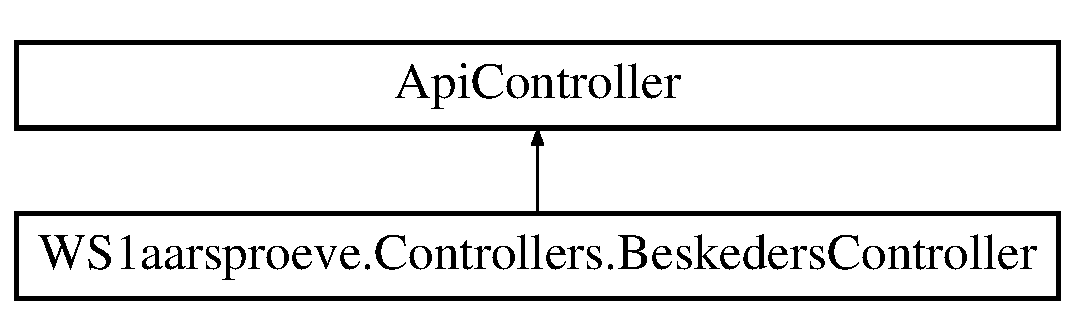
\includegraphics[height=2.000000cm]{class_w_s1aarsproeve_1_1_controllers_1_1_beskeders_controller}
\end{center}
\end{figure}
\subsection*{Public Member Functions}
\begin{DoxyCompactItemize}
\item 
\hypertarget{class_w_s1aarsproeve_1_1_controllers_1_1_beskeders_controller_a4040005e2a34cbaa959ea7e5957500c0}{}I\+Queryable$<$ \hyperlink{class_w_s1aarsproeve_1_1_beskeder}{Beskeder} $>$ {\bfseries Get\+Beskeders} ()\label{class_w_s1aarsproeve_1_1_controllers_1_1_beskeders_controller_a4040005e2a34cbaa959ea7e5957500c0}

\item 
\hypertarget{class_w_s1aarsproeve_1_1_controllers_1_1_beskeders_controller_abe70f47b2f3911726fb9b7f0bf8c3e3d}{}I\+Http\+Action\+Result {\bfseries Get\+Beskeder} (int id)\label{class_w_s1aarsproeve_1_1_controllers_1_1_beskeders_controller_abe70f47b2f3911726fb9b7f0bf8c3e3d}

\item 
\hypertarget{class_w_s1aarsproeve_1_1_controllers_1_1_beskeders_controller_a0069b70d45069d85445d7435fb29c23e}{}I\+Http\+Action\+Result {\bfseries Put\+Beskeder} (int id, \hyperlink{class_w_s1aarsproeve_1_1_beskeder}{Beskeder} beskeder)\label{class_w_s1aarsproeve_1_1_controllers_1_1_beskeders_controller_a0069b70d45069d85445d7435fb29c23e}

\item 
\hypertarget{class_w_s1aarsproeve_1_1_controllers_1_1_beskeders_controller_a0e616763464095dcf83536a282c12701}{}I\+Http\+Action\+Result {\bfseries Post\+Beskeder} (\hyperlink{class_w_s1aarsproeve_1_1_beskeder}{Beskeder} beskeder)\label{class_w_s1aarsproeve_1_1_controllers_1_1_beskeders_controller_a0e616763464095dcf83536a282c12701}

\item 
\hypertarget{class_w_s1aarsproeve_1_1_controllers_1_1_beskeders_controller_ab5c7f26e503324a054c2761b21a2b092}{}I\+Http\+Action\+Result {\bfseries Delete\+Beskeder} (int id)\label{class_w_s1aarsproeve_1_1_controllers_1_1_beskeders_controller_ab5c7f26e503324a054c2761b21a2b092}

\end{DoxyCompactItemize}
\subsection*{Protected Member Functions}
\begin{DoxyCompactItemize}
\item 
\hypertarget{class_w_s1aarsproeve_1_1_controllers_1_1_beskeders_controller_a381d5cf463ae84115d93dc66dfe201a4}{}override void {\bfseries Dispose} (bool disposing)\label{class_w_s1aarsproeve_1_1_controllers_1_1_beskeders_controller_a381d5cf463ae84115d93dc66dfe201a4}

\end{DoxyCompactItemize}


The documentation for this class was generated from the following file\+:\begin{DoxyCompactItemize}
\item 
Documents/\+Git\+Hub/1-\/aarsproeve/1aarsproeve/\+W\+S1aarsproeve/\+Controllers/Beskeders\+Controller.\+cs\end{DoxyCompactItemize}

\hypertarget{class__1aarsproeve_tests_1_1_beskeder_tests}{}\section{\+\_\+1aarsproeve\+Tests.\+Beskeder\+Tests Class Reference}
\label{class__1aarsproeve_tests_1_1_beskeder_tests}\index{\+\_\+1aarsproeve\+Tests.\+Beskeder\+Tests@{\+\_\+1aarsproeve\+Tests.\+Beskeder\+Tests}}
\subsection*{Public Member Functions}
\begin{DoxyCompactItemize}
\item 
\hypertarget{class__1aarsproeve_tests_1_1_beskeder_tests_a776cf61b3ba30a23d81b45b8b3a8bb16}{}void {\bfseries Before\+Test} ()\label{class__1aarsproeve_tests_1_1_beskeder_tests_a776cf61b3ba30a23d81b45b8b3a8bb16}

\item 
\hypertarget{class__1aarsproeve_tests_1_1_beskeder_tests_ad8b21a2660bf697e9c9de677b2bbf0b2}{}void {\bfseries Check\+Beskrivelse\+Test} ()\label{class__1aarsproeve_tests_1_1_beskeder_tests_ad8b21a2660bf697e9c9de677b2bbf0b2}

\item 
\hypertarget{class__1aarsproeve_tests_1_1_beskeder_tests_a6395cf468a8710a0e8fff9c917a46955}{}void {\bfseries Check\+Beskrivelse\+Test1} ()\label{class__1aarsproeve_tests_1_1_beskeder_tests_a6395cf468a8710a0e8fff9c917a46955}

\item 
\hypertarget{class__1aarsproeve_tests_1_1_beskeder_tests_a1b6964f1eba00f29782962d1e3429de6}{}void {\bfseries Check\+Beskrivelse\+Test2} ()\label{class__1aarsproeve_tests_1_1_beskeder_tests_a1b6964f1eba00f29782962d1e3429de6}

\item 
\hypertarget{class__1aarsproeve_tests_1_1_beskeder_tests_a221c18ee3ade362f2b40063dc7f7ebcb}{}void {\bfseries Check\+Beskrivelse\+Test3} ()\label{class__1aarsproeve_tests_1_1_beskeder_tests_a221c18ee3ade362f2b40063dc7f7ebcb}

\item 
\hypertarget{class__1aarsproeve_tests_1_1_beskeder_tests_a82ebe5a34a90753eca52830583786a9b}{}void {\bfseries Check\+Brugernavn\+Test} ()\label{class__1aarsproeve_tests_1_1_beskeder_tests_a82ebe5a34a90753eca52830583786a9b}

\item 
\hypertarget{class__1aarsproeve_tests_1_1_beskeder_tests_ae2d9ebd3354683c7d606e18b760ceaea}{}void {\bfseries Check\+Brugernavn\+Test1} ()\label{class__1aarsproeve_tests_1_1_beskeder_tests_ae2d9ebd3354683c7d606e18b760ceaea}

\item 
\hypertarget{class__1aarsproeve_tests_1_1_beskeder_tests_ac1e31fb7754f6447173b6ce4419f3ad6}{}void {\bfseries Check\+Brugernavn\+Test2} ()\label{class__1aarsproeve_tests_1_1_beskeder_tests_ac1e31fb7754f6447173b6ce4419f3ad6}

\item 
\hypertarget{class__1aarsproeve_tests_1_1_beskeder_tests_a954cde8ed5c377f48d789b62f39f3002}{}void {\bfseries Check\+Overskrift\+Test} ()\label{class__1aarsproeve_tests_1_1_beskeder_tests_a954cde8ed5c377f48d789b62f39f3002}

\item 
\hypertarget{class__1aarsproeve_tests_1_1_beskeder_tests_af62386631da03f574b14c45540eef027}{}void {\bfseries Check\+Overskrift\+Test1} ()\label{class__1aarsproeve_tests_1_1_beskeder_tests_af62386631da03f574b14c45540eef027}

\item 
\hypertarget{class__1aarsproeve_tests_1_1_beskeder_tests_afb39a7419f9b9c2296c56b886e937c65}{}void {\bfseries Check\+Overskrift\+Test2} ()\label{class__1aarsproeve_tests_1_1_beskeder_tests_afb39a7419f9b9c2296c56b886e937c65}

\item 
\hypertarget{class__1aarsproeve_tests_1_1_beskeder_tests_a8406aba23c7c546f0695457e535a3162}{}void {\bfseries Check\+Overskrift\+Test3} ()\label{class__1aarsproeve_tests_1_1_beskeder_tests_a8406aba23c7c546f0695457e535a3162}

\end{DoxyCompactItemize}


The documentation for this class was generated from the following file\+:\begin{DoxyCompactItemize}
\item 
Documents/\+Git\+Hub/1-\/aarsproeve/1aarsproeve/1aarsproeve\+Tests/Beskeder\+Tests.\+cs\end{DoxyCompactItemize}

\hypertarget{class__1aarsproeve_1_1_view_model_1_1_bruger_view_model}{}\section{\+\_\+1aarsproeve.\+View\+Model.\+Bruger\+View\+Model Class Reference}
\label{class__1aarsproeve_1_1_view_model_1_1_bruger_view_model}\index{\+\_\+1aarsproeve.\+View\+Model.\+Bruger\+View\+Model@{\+\_\+1aarsproeve.\+View\+Model.\+Bruger\+View\+Model}}
\subsection*{Public Member Functions}
\begin{DoxyCompactItemize}
\item 
\hypertarget{class__1aarsproeve_1_1_view_model_1_1_bruger_view_model_a8c2d6da5fad3a9bdbbde9ce986dcbc74}{}void {\bfseries Log\+Ud} ()\label{class__1aarsproeve_1_1_view_model_1_1_bruger_view_model_a8c2d6da5fad3a9bdbbde9ce986dcbc74}

\end{DoxyCompactItemize}
\subsection*{Properties}
\begin{DoxyCompactItemize}
\item 
\hypertarget{class__1aarsproeve_1_1_view_model_1_1_bruger_view_model_ac9e91065596a741027a1b88853bd76e6}{}Application\+Data\+Container {\bfseries Setting}\hspace{0.3cm}{\ttfamily  \mbox{[}get, set\mbox{]}}\label{class__1aarsproeve_1_1_view_model_1_1_bruger_view_model_ac9e91065596a741027a1b88853bd76e6}

\item 
\hypertarget{class__1aarsproeve_1_1_view_model_1_1_bruger_view_model_a63b4a8aa59a8e3e2ec0d7285c2ce6caa}{}string {\bfseries Brugernavn}\hspace{0.3cm}{\ttfamily  \mbox{[}get, set\mbox{]}}\label{class__1aarsproeve_1_1_view_model_1_1_bruger_view_model_a63b4a8aa59a8e3e2ec0d7285c2ce6caa}

\item 
\hypertarget{class__1aarsproeve_1_1_view_model_1_1_bruger_view_model_a40fed761861b9387bc47a92a2f1e55fd}{}I\+Command {\bfseries Log\+Ind\+Command}\hspace{0.3cm}{\ttfamily  \mbox{[}get, set\mbox{]}}\label{class__1aarsproeve_1_1_view_model_1_1_bruger_view_model_a40fed761861b9387bc47a92a2f1e55fd}

\item 
\hypertarget{class__1aarsproeve_1_1_view_model_1_1_bruger_view_model_afc1d332a62edcc717d3e1764db42c89a}{}I\+Command {\bfseries Log\+Ud\+Command}\hspace{0.3cm}{\ttfamily  \mbox{[}get, set\mbox{]}}\label{class__1aarsproeve_1_1_view_model_1_1_bruger_view_model_afc1d332a62edcc717d3e1764db42c89a}

\end{DoxyCompactItemize}


The documentation for this class was generated from the following file\+:\begin{DoxyCompactItemize}
\item 
C\+:/\+Users/\+Daniel\+Winther/\+Documents/\+Git\+Hub/1-\/aarsproeve/1aarsproeve/1aarsproeve/\+View\+Model/Bruger\+View\+Model.\+cs\end{DoxyCompactItemize}

\hypertarget{class_w_s1aarsproeve_1_1_bundle_config}{}\section{W\+S1aarsproeve.\+Bundle\+Config Class Reference}
\label{class_w_s1aarsproeve_1_1_bundle_config}\index{W\+S1aarsproeve.\+Bundle\+Config@{W\+S1aarsproeve.\+Bundle\+Config}}
\subsection*{Static Public Member Functions}
\begin{DoxyCompactItemize}
\item 
\hypertarget{class_w_s1aarsproeve_1_1_bundle_config_a72934e29affaa05806c1b6d9e1779f7b}{}static void {\bfseries Register\+Bundles} (Bundle\+Collection bundles)\label{class_w_s1aarsproeve_1_1_bundle_config_a72934e29affaa05806c1b6d9e1779f7b}

\end{DoxyCompactItemize}


The documentation for this class was generated from the following file\+:\begin{DoxyCompactItemize}
\item 
Documents/\+Git\+Hub/1-\/aarsproeve/1aarsproeve/\+W\+S1aarsproeve/\+App\+\_\+\+Start/Bundle\+Config.\+cs\end{DoxyCompactItemize}

\hypertarget{class__1aarsproeve_web_service_1_1_bundle_config}{}\section{\+\_\+1aarsproeve\+Web\+Service.\+Bundle\+Config Class Reference}
\label{class__1aarsproeve_web_service_1_1_bundle_config}\index{\+\_\+1aarsproeve\+Web\+Service.\+Bundle\+Config@{\+\_\+1aarsproeve\+Web\+Service.\+Bundle\+Config}}
\subsection*{Static Public Member Functions}
\begin{DoxyCompactItemize}
\item 
\hypertarget{class__1aarsproeve_web_service_1_1_bundle_config_ab9a18fe210fb037e3bdb7405a0b456e6}{}static void {\bfseries Register\+Bundles} (Bundle\+Collection bundles)\label{class__1aarsproeve_web_service_1_1_bundle_config_ab9a18fe210fb037e3bdb7405a0b456e6}

\end{DoxyCompactItemize}


The documentation for this class was generated from the following file\+:\begin{DoxyCompactItemize}
\item 
C\+:/\+Users/\+Daniel\+Winther/\+Documents/\+Git\+Hub/1-\/aarsproeve/1aarsproeve/1aarsproeve\+Web\+Service/\+App\+\_\+\+Start/Bundle\+Config.\+cs\end{DoxyCompactItemize}

\hypertarget{class__1aarsproeve_1_1_annotations_1_1_can_be_null_attribute}{}\section{\+\_\+1aarsproeve.\+Annotations.\+Can\+Be\+Null\+Attribute Class Reference}
\label{class__1aarsproeve_1_1_annotations_1_1_can_be_null_attribute}\index{\+\_\+1aarsproeve.\+Annotations.\+Can\+Be\+Null\+Attribute@{\+\_\+1aarsproeve.\+Annotations.\+Can\+Be\+Null\+Attribute}}


Indicates that the value of the marked element could be {\ttfamily null} sometimes, so the check for {\ttfamily null} is necessary before its usage  


Inheritance diagram for \+\_\+1aarsproeve.\+Annotations.\+Can\+Be\+Null\+Attribute\+:\begin{figure}[H]
\begin{center}
\leavevmode
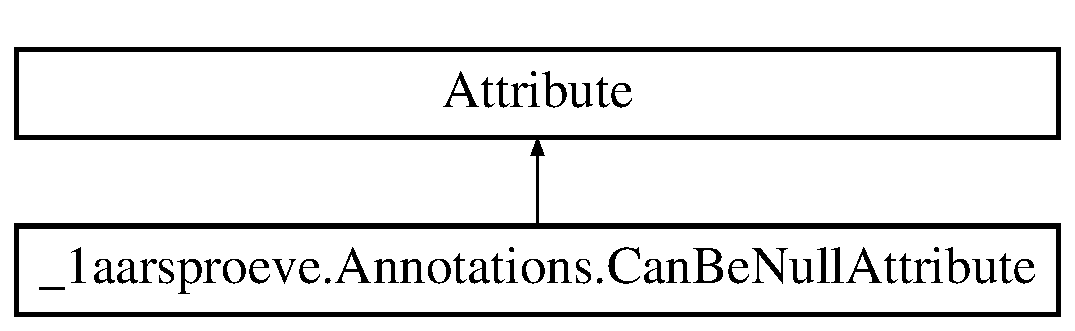
\includegraphics[height=2.000000cm]{class__1aarsproeve_1_1_annotations_1_1_can_be_null_attribute}
\end{center}
\end{figure}


\subsection{Detailed Description}
Indicates that the value of the marked element could be {\ttfamily null} sometimes, so the check for {\ttfamily null} is necessary before its usage 


\begin{DoxyCode}
[CanBeNull] \textcolor{keyword}{public} \textcolor{keywordtype}{object} Test() \{ \textcolor{keywordflow}{return} null; \}
\textcolor{keyword}{public} \textcolor{keywordtype}{void} UseTest() \{
  var p = Test();
  var s = p.ToString(); \textcolor{comment}{// Warning: Possible 'System.NullReferenceException'}
\}
\end{DoxyCode}


The documentation for this class was generated from the following file\+:\begin{DoxyCompactItemize}
\item 
Documents/\+Git\+Hub/1-\/aarsproeve/1aarsproeve/1aarsproeve/\+Properties/Annotations.\+cs\end{DoxyCompactItemize}

\hypertarget{class_cannot_apply_equality_operator_attribute}{}\section{Cannot\+Apply\+Equality\+Operator\+Attribute Class Reference}
\label{class_cannot_apply_equality_operator_attribute}\index{Cannot\+Apply\+Equality\+Operator\+Attribute@{Cannot\+Apply\+Equality\+Operator\+Attribute}}


Indicates that the value of the marked type (or its derivatives) cannot be compared using \textquotesingle{}==\textquotesingle{} or \textquotesingle{}!=\textquotesingle{} operators and {\ttfamily Equals()} should be used instead. However, using \textquotesingle{}==\textquotesingle{} or \textquotesingle{}!=\textquotesingle{} for comparison with {\ttfamily null} is always permitted.  


Inheritance diagram for Cannot\+Apply\+Equality\+Operator\+Attribute\+:\begin{figure}[H]
\begin{center}
\leavevmode
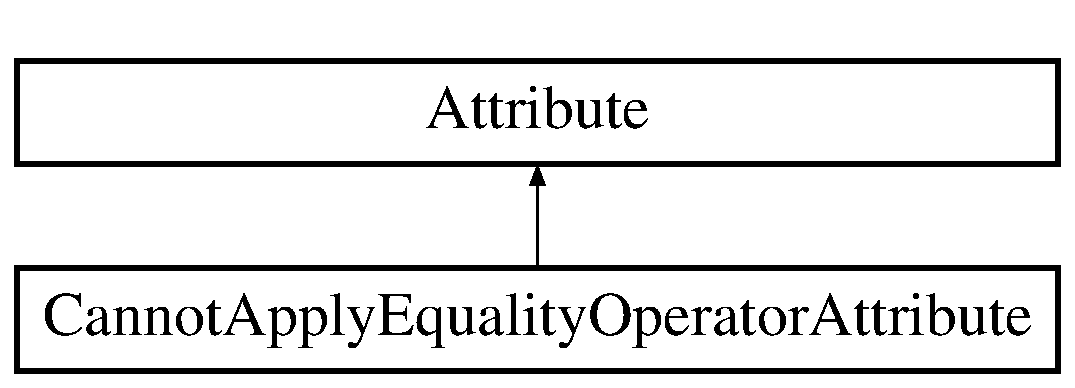
\includegraphics[height=2.000000cm]{class_cannot_apply_equality_operator_attribute}
\end{center}
\end{figure}


\subsection{Detailed Description}
Indicates that the value of the marked type (or its derivatives) cannot be compared using \textquotesingle{}==\textquotesingle{} or \textquotesingle{}!=\textquotesingle{} operators and {\ttfamily Equals()} should be used instead. However, using \textquotesingle{}==\textquotesingle{} or \textquotesingle{}!=\textquotesingle{} for comparison with {\ttfamily null} is always permitted. 


\begin{DoxyCode}
[CannotApplyEqualityOperator]
\textcolor{keyword}{class }NoEquality \{ \}
\textcolor{keyword}{class }UsesNoEquality \{
  \textcolor{keyword}{public} \textcolor{keywordtype}{void} Test() \{
    var ca1 = \textcolor{keyword}{new} NoEquality();
    var ca2 = \textcolor{keyword}{new} NoEquality();
    \textcolor{keywordflow}{if} (ca1 != null) \{ \textcolor{comment}{// OK}
      \textcolor{keywordtype}{bool} condition = ca1 == ca2; \textcolor{comment}{// Warning}
    \}
  \}
\}
\end{DoxyCode}


The documentation for this class was generated from the following file\+:\begin{DoxyCompactItemize}
\item 
Documents/\+Git\+Hub/1-\/aarsproeve/1aarsproeve/1aarsproeve/\+Properties/Annotations.\+cs\end{DoxyCompactItemize}

\hypertarget{class_collection_access_attribute}{}\section{Collection\+Access\+Attribute Class Reference}
\label{class_collection_access_attribute}\index{Collection\+Access\+Attribute@{Collection\+Access\+Attribute}}


Indicates how method invocation affects content of the collection  


Inheritance diagram for Collection\+Access\+Attribute\+:\begin{figure}[H]
\begin{center}
\leavevmode
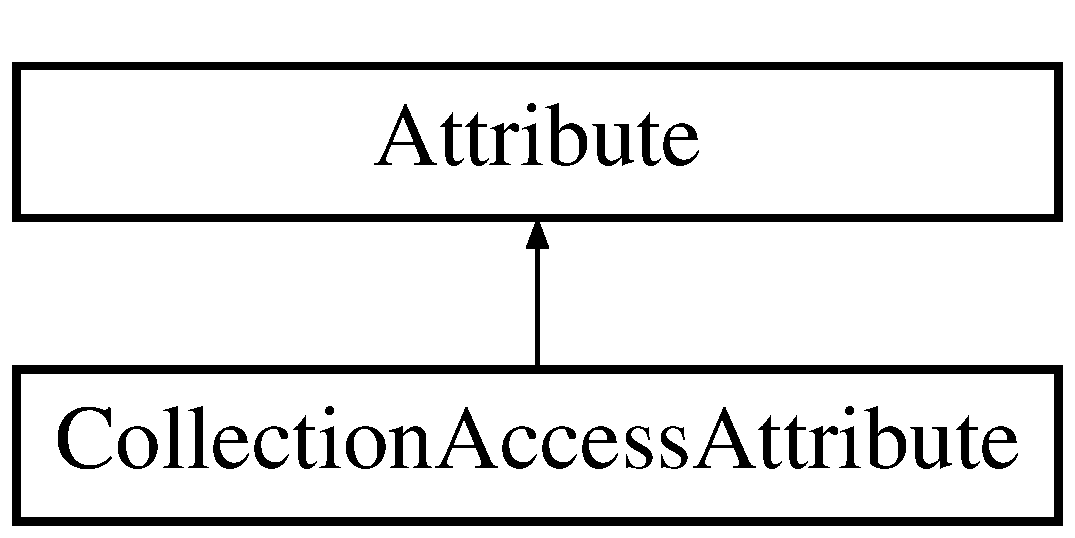
\includegraphics[height=2.000000cm]{class_collection_access_attribute}
\end{center}
\end{figure}
\subsection*{Public Member Functions}
\begin{DoxyCompactItemize}
\item 
\hypertarget{class_collection_access_attribute_a14445128bbc836c5876b84ac71307e91}{}{\bfseries Collection\+Access\+Attribute} (Collection\+Access\+Type collection\+Access\+Type)\label{class_collection_access_attribute_a14445128bbc836c5876b84ac71307e91}

\end{DoxyCompactItemize}
\subsection*{Properties}
\begin{DoxyCompactItemize}
\item 
\hypertarget{class_collection_access_attribute_a6f4227ee9e50c5103d73637cef1a3a9e}{}Collection\+Access\+Type {\bfseries Collection\+Access\+Type}\hspace{0.3cm}{\ttfamily  \mbox{[}get\mbox{]}}\label{class_collection_access_attribute_a6f4227ee9e50c5103d73637cef1a3a9e}

\end{DoxyCompactItemize}


\subsection{Detailed Description}
Indicates how method invocation affects content of the collection 



The documentation for this class was generated from the following file\+:\begin{DoxyCompactItemize}
\item 
Documents/\+Git\+Hub/1-\/aarsproeve/1aarsproeve/1aarsproeve/\+Properties/Annotations.\+cs\end{DoxyCompactItemize}

\hypertarget{class_w_s1aarsproeve_1_1_areas_1_1_help_page_1_1_model_descriptions_1_1_collection_model_description}{}\section{W\+S1aarsproeve.\+Areas.\+Help\+Page.\+Model\+Descriptions.\+Collection\+Model\+Description Class Reference}
\label{class_w_s1aarsproeve_1_1_areas_1_1_help_page_1_1_model_descriptions_1_1_collection_model_description}\index{W\+S1aarsproeve.\+Areas.\+Help\+Page.\+Model\+Descriptions.\+Collection\+Model\+Description@{W\+S1aarsproeve.\+Areas.\+Help\+Page.\+Model\+Descriptions.\+Collection\+Model\+Description}}
Inheritance diagram for W\+S1aarsproeve.\+Areas.\+Help\+Page.\+Model\+Descriptions.\+Collection\+Model\+Description\+:\begin{figure}[H]
\begin{center}
\leavevmode
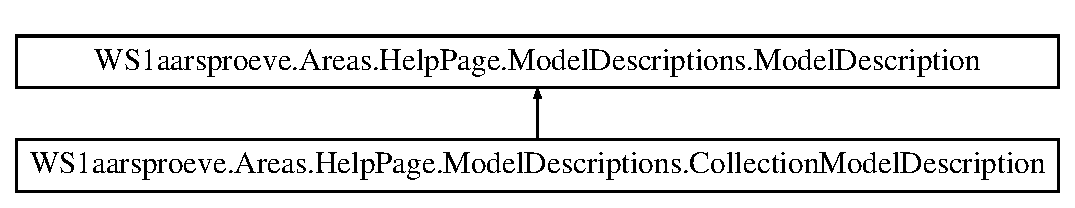
\includegraphics[height=2.000000cm]{class_w_s1aarsproeve_1_1_areas_1_1_help_page_1_1_model_descriptions_1_1_collection_model_description}
\end{center}
\end{figure}
\subsection*{Properties}
\begin{DoxyCompactItemize}
\item 
\hypertarget{class_w_s1aarsproeve_1_1_areas_1_1_help_page_1_1_model_descriptions_1_1_collection_model_description_a6c7988db6c5bcba24f586ea0ed0d14cc}{}\hyperlink{class_w_s1aarsproeve_1_1_areas_1_1_help_page_1_1_model_descriptions_1_1_model_description}{Model\+Description} {\bfseries Element\+Description}\hspace{0.3cm}{\ttfamily  \mbox{[}get, set\mbox{]}}\label{class_w_s1aarsproeve_1_1_areas_1_1_help_page_1_1_model_descriptions_1_1_collection_model_description_a6c7988db6c5bcba24f586ea0ed0d14cc}

\end{DoxyCompactItemize}


The documentation for this class was generated from the following file\+:\begin{DoxyCompactItemize}
\item 
Documents/\+Git\+Hub/1-\/aarsproeve/1aarsproeve/\+W\+S1aarsproeve/\+Areas/\+Help\+Page/\+Model\+Descriptions/Collection\+Model\+Description.\+cs\end{DoxyCompactItemize}

\hypertarget{class__1aarsproeve_web_service_1_1_areas_1_1_help_page_1_1_model_descriptions_1_1_collection_model_description}{}\section{\+\_\+1aarsproeve\+Web\+Service.\+Areas.\+Help\+Page.\+Model\+Descriptions.\+Collection\+Model\+Description Class Reference}
\label{class__1aarsproeve_web_service_1_1_areas_1_1_help_page_1_1_model_descriptions_1_1_collection_model_description}\index{\+\_\+1aarsproeve\+Web\+Service.\+Areas.\+Help\+Page.\+Model\+Descriptions.\+Collection\+Model\+Description@{\+\_\+1aarsproeve\+Web\+Service.\+Areas.\+Help\+Page.\+Model\+Descriptions.\+Collection\+Model\+Description}}
Inheritance diagram for \+\_\+1aarsproeve\+Web\+Service.\+Areas.\+Help\+Page.\+Model\+Descriptions.\+Collection\+Model\+Description\+:\begin{figure}[H]
\begin{center}
\leavevmode
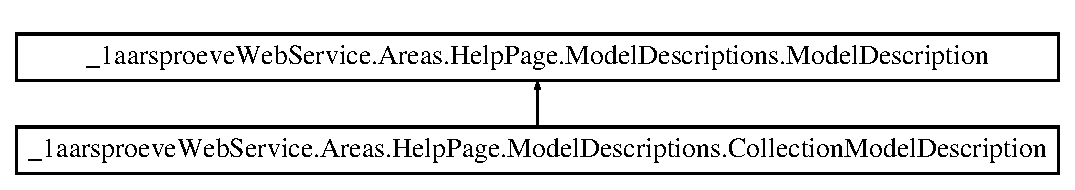
\includegraphics[height=2.000000cm]{class__1aarsproeve_web_service_1_1_areas_1_1_help_page_1_1_model_descriptions_1_1_collection_model_description}
\end{center}
\end{figure}
\subsection*{Properties}
\begin{DoxyCompactItemize}
\item 
\hypertarget{class__1aarsproeve_web_service_1_1_areas_1_1_help_page_1_1_model_descriptions_1_1_collection_model_description_a9f59a1485146c386bb767ff88380e3b2}{}\hyperlink{class__1aarsproeve_web_service_1_1_areas_1_1_help_page_1_1_model_descriptions_1_1_model_description}{Model\+Description} {\bfseries Element\+Description}\hspace{0.3cm}{\ttfamily  \mbox{[}get, set\mbox{]}}\label{class__1aarsproeve_web_service_1_1_areas_1_1_help_page_1_1_model_descriptions_1_1_collection_model_description_a9f59a1485146c386bb767ff88380e3b2}

\end{DoxyCompactItemize}


The documentation for this class was generated from the following file\+:\begin{DoxyCompactItemize}
\item 
Documents/\+Git\+Hub/1-\/aarsproeve/1aarsproeve/1aarsproeve\+Web\+Service/\+Areas/\+Help\+Page/\+Model\+Descriptions/Collection\+Model\+Description.\+cs\end{DoxyCompactItemize}

\hypertarget{class_w_s1aarsproeve_1_1_areas_1_1_help_page_1_1_model_descriptions_1_1_complex_type_model_description}{}\section{W\+S1aarsproeve.\+Areas.\+Help\+Page.\+Model\+Descriptions.\+Complex\+Type\+Model\+Description Class Reference}
\label{class_w_s1aarsproeve_1_1_areas_1_1_help_page_1_1_model_descriptions_1_1_complex_type_model_description}\index{W\+S1aarsproeve.\+Areas.\+Help\+Page.\+Model\+Descriptions.\+Complex\+Type\+Model\+Description@{W\+S1aarsproeve.\+Areas.\+Help\+Page.\+Model\+Descriptions.\+Complex\+Type\+Model\+Description}}
Inheritance diagram for W\+S1aarsproeve.\+Areas.\+Help\+Page.\+Model\+Descriptions.\+Complex\+Type\+Model\+Description\+:\begin{figure}[H]
\begin{center}
\leavevmode
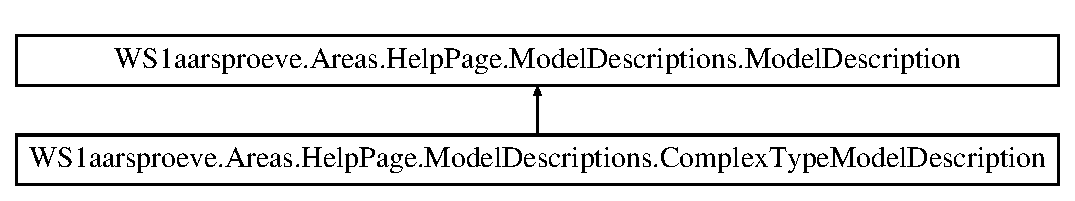
\includegraphics[height=2.000000cm]{class_w_s1aarsproeve_1_1_areas_1_1_help_page_1_1_model_descriptions_1_1_complex_type_model_description}
\end{center}
\end{figure}
\subsection*{Properties}
\begin{DoxyCompactItemize}
\item 
\hypertarget{class_w_s1aarsproeve_1_1_areas_1_1_help_page_1_1_model_descriptions_1_1_complex_type_model_description_a2ce892eed85c4d483831d0eba9557a0b}{}Collection$<$ \hyperlink{class_w_s1aarsproeve_1_1_areas_1_1_help_page_1_1_model_descriptions_1_1_parameter_description}{Parameter\+Description} $>$ {\bfseries Properties}\hspace{0.3cm}{\ttfamily  \mbox{[}get\mbox{]}}\label{class_w_s1aarsproeve_1_1_areas_1_1_help_page_1_1_model_descriptions_1_1_complex_type_model_description_a2ce892eed85c4d483831d0eba9557a0b}

\end{DoxyCompactItemize}


The documentation for this class was generated from the following file\+:\begin{DoxyCompactItemize}
\item 
Documents/\+Git\+Hub/1-\/aarsproeve/1aarsproeve/\+W\+S1aarsproeve/\+Areas/\+Help\+Page/\+Model\+Descriptions/Complex\+Type\+Model\+Description.\+cs\end{DoxyCompactItemize}

\hypertarget{class__1aarsproeve_web_service_1_1_areas_1_1_help_page_1_1_model_descriptions_1_1_complex_type_model_description}{}\section{\+\_\+1aarsproeve\+Web\+Service.\+Areas.\+Help\+Page.\+Model\+Descriptions.\+Complex\+Type\+Model\+Description Class Reference}
\label{class__1aarsproeve_web_service_1_1_areas_1_1_help_page_1_1_model_descriptions_1_1_complex_type_model_description}\index{\+\_\+1aarsproeve\+Web\+Service.\+Areas.\+Help\+Page.\+Model\+Descriptions.\+Complex\+Type\+Model\+Description@{\+\_\+1aarsproeve\+Web\+Service.\+Areas.\+Help\+Page.\+Model\+Descriptions.\+Complex\+Type\+Model\+Description}}
Inheritance diagram for \+\_\+1aarsproeve\+Web\+Service.\+Areas.\+Help\+Page.\+Model\+Descriptions.\+Complex\+Type\+Model\+Description\+:\begin{figure}[H]
\begin{center}
\leavevmode
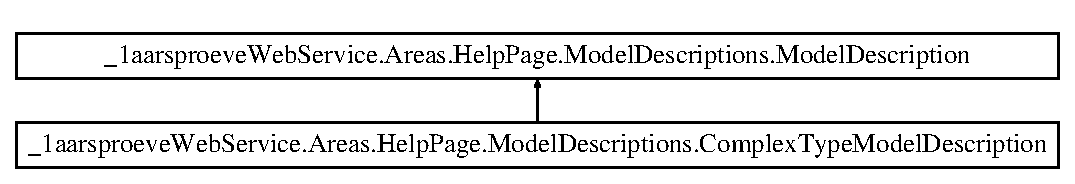
\includegraphics[height=2.000000cm]{class__1aarsproeve_web_service_1_1_areas_1_1_help_page_1_1_model_descriptions_1_1_complex_type_model_description}
\end{center}
\end{figure}
\subsection*{Properties}
\begin{DoxyCompactItemize}
\item 
\hypertarget{class__1aarsproeve_web_service_1_1_areas_1_1_help_page_1_1_model_descriptions_1_1_complex_type_model_description_afabdec8e2987c716ec40a6d32410fca9}{}Collection$<$ \hyperlink{class__1aarsproeve_web_service_1_1_areas_1_1_help_page_1_1_model_descriptions_1_1_parameter_description}{Parameter\+Description} $>$ {\bfseries Properties}\hspace{0.3cm}{\ttfamily  \mbox{[}get\mbox{]}}\label{class__1aarsproeve_web_service_1_1_areas_1_1_help_page_1_1_model_descriptions_1_1_complex_type_model_description_afabdec8e2987c716ec40a6d32410fca9}

\end{DoxyCompactItemize}


The documentation for this class was generated from the following file\+:\begin{DoxyCompactItemize}
\item 
C\+:/\+Users/\+Daniel\+Winther/\+Documents/\+Git\+Hub/1-\/aarsproeve/1aarsproeve/1aarsproeve\+Web\+Service/\+Areas/\+Help\+Page/\+Model\+Descriptions/Complex\+Type\+Model\+Description.\+cs\end{DoxyCompactItemize}

\hypertarget{class_contract_annotation_attribute}{}\section{Contract\+Annotation\+Attribute Class Reference}
\label{class_contract_annotation_attribute}\index{Contract\+Annotation\+Attribute@{Contract\+Annotation\+Attribute}}


Describes dependency between method input and output  


Inheritance diagram for Contract\+Annotation\+Attribute\+:\begin{figure}[H]
\begin{center}
\leavevmode
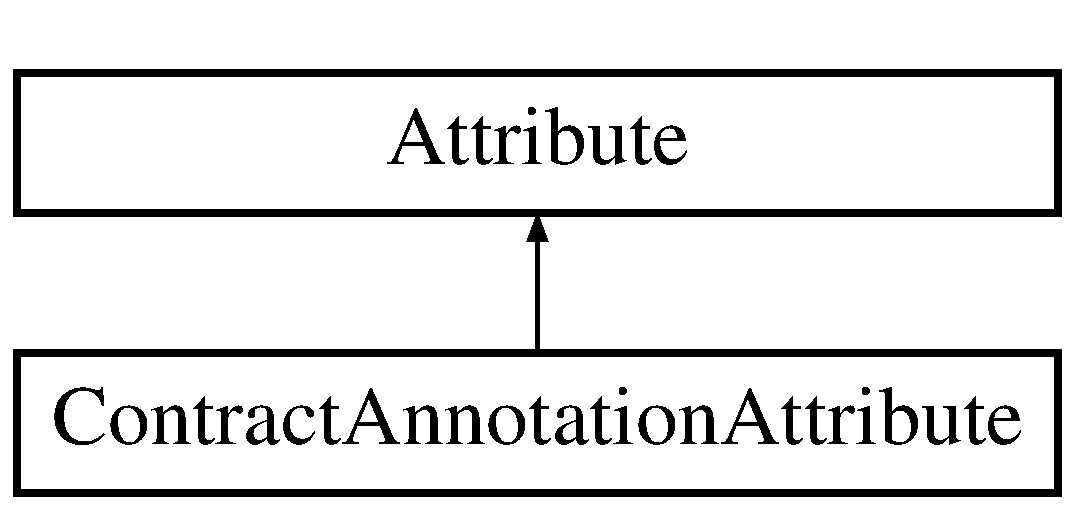
\includegraphics[height=2.000000cm]{class_contract_annotation_attribute}
\end{center}
\end{figure}
\subsection*{Public Member Functions}
\begin{DoxyCompactItemize}
\item 
\hypertarget{class_contract_annotation_attribute_a635552c48df4e94f26deb7598f7a5028}{}{\bfseries Contract\+Annotation\+Attribute} (\mbox{[}Not\+Null\mbox{]} string contract)\label{class_contract_annotation_attribute_a635552c48df4e94f26deb7598f7a5028}

\item 
\hypertarget{class_contract_annotation_attribute_a886eedce3d8c7a269549a3293a2bfd99}{}{\bfseries Contract\+Annotation\+Attribute} (\mbox{[}Not\+Null\mbox{]} string contract, bool force\+Full\+States)\label{class_contract_annotation_attribute_a886eedce3d8c7a269549a3293a2bfd99}

\end{DoxyCompactItemize}
\subsection*{Properties}
\begin{DoxyCompactItemize}
\item 
\hypertarget{class_contract_annotation_attribute_a19445968a4365371890d047311eaa1c4}{}string {\bfseries Contract}\hspace{0.3cm}{\ttfamily  \mbox{[}get\mbox{]}}\label{class_contract_annotation_attribute_a19445968a4365371890d047311eaa1c4}

\item 
\hypertarget{class_contract_annotation_attribute_a329c6f99fe2ed0c08df3898586cbf965}{}bool {\bfseries Force\+Full\+States}\hspace{0.3cm}{\ttfamily  \mbox{[}get\mbox{]}}\label{class_contract_annotation_attribute_a329c6f99fe2ed0c08df3898586cbf965}

\end{DoxyCompactItemize}


\subsection{Detailed Description}
Describes dependency between method input and output 

$<$syntax$>$ 

Function Definition Table syntax\+:


\begin{DoxyItemize}
\item F\+D\+T \+:\+:= F\+D\+T\+Row \mbox{[};F\+D\+T\+Row\mbox{]}$\ast$ 
\item F\+D\+T\+Row \+:\+:= Input =$>$ Output $\vert$ Output $<$= Input 
\item Input \+:\+:= Parameter\+Name\+: Value \mbox{[}, Input\mbox{]}$\ast$ 
\item Output \+:\+:= \mbox{[}Parameter\+Name\+: Value\mbox{]}$\ast$ \{halt$\vert$stop$\vert$void$\vert$nothing$\vert$\+Value\} 
\item Value \+:\+:= true $\vert$ false $\vert$ null $\vert$ notnull $\vert$ canbenull 
\end{DoxyItemize}If method has single input parameter, it\textquotesingle{}s name could be omitted.~\newline
 Using {\ttfamily halt} (or {\ttfamily void}/{\ttfamily nothing}, which is the same) for method output means that the methos doesn\textquotesingle{}t return normally.~\newline
 {\ttfamily canbenull} annotation is only applicable for output parameters.~\newline
 You can use multiple {\ttfamily \mbox{[}Contract\+Annotation\mbox{]}} for each F\+D\+T row, or use single attribute with rows separated by semicolon.~\newline
 $<$/syntax$>$ $<$examples$>$
\begin{DoxyItemize}
\item {\ttfamily  \mbox{[}Contract\+Annotation(\char`\"{}=$>$ halt\char`\"{})\mbox{]} public void Termination\+Method() } 
\item {\ttfamily  \mbox{[}Contract\+Annotation(\char`\"{}halt \&lt;= condition\+: false\char`\"{})\mbox{]} public void Assert(bool condition, string text) // regular assertion method } 
\item {\ttfamily  \mbox{[}Contract\+Annotation(\char`\"{}s\+:null =$>$ true\char`\"{})\mbox{]} public bool Is\+Null\+Or\+Empty(string s) // string.\+Is\+Null\+Or\+Empty() } 
\item {\ttfamily  // A method that returns null if the parameter is null, // and not null if the parameter is not null \mbox{[}Contract\+Annotation(\char`\"{}null =$>$ null; notnull =$>$ notnull\char`\"{})\mbox{]} public object Transform(object data) } 
\item {\ttfamily  \mbox{[}Contract\+Annotation(\char`\"{}s\+:null=$>$false; =$>$true,result\+:notnull; =$>$false, result\+:null\char`\"{})\mbox{]} public bool Try\+Parse(string s, out Person result) } 
\end{DoxyItemize}$<$/examples$>$ 

The documentation for this class was generated from the following file\+:\begin{DoxyCompactItemize}
\item 
Documents/\+Git\+Hub/1-\/aarsproeve/1aarsproeve/1aarsproeve/\+Properties/Annotations.\+cs\end{DoxyCompactItemize}

\hypertarget{class__1aarsproeve_web_service_1_1_data_table_context}{}\section{\+\_\+1aarsproeve\+Web\+Service.\+Data\+Table\+Context Class Reference}
\label{class__1aarsproeve_web_service_1_1_data_table_context}\index{\+\_\+1aarsproeve\+Web\+Service.\+Data\+Table\+Context@{\+\_\+1aarsproeve\+Web\+Service.\+Data\+Table\+Context}}
Inheritance diagram for \+\_\+1aarsproeve\+Web\+Service.\+Data\+Table\+Context\+:\begin{figure}[H]
\begin{center}
\leavevmode
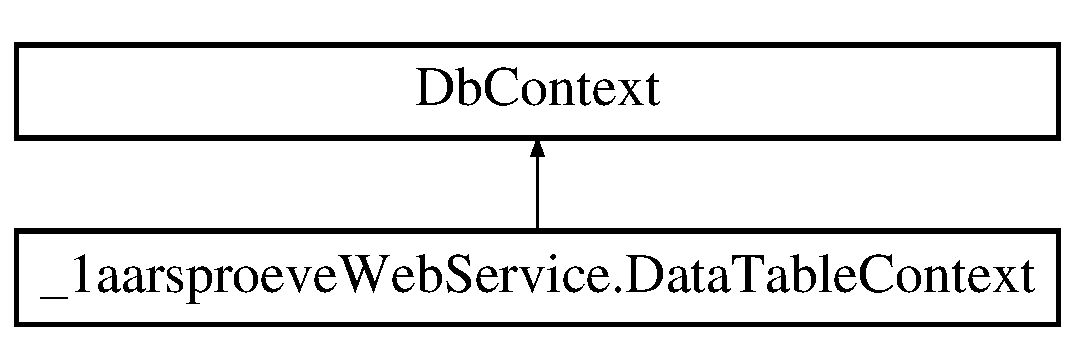
\includegraphics[height=2.000000cm]{class__1aarsproeve_web_service_1_1_data_table_context}
\end{center}
\end{figure}
\subsection*{Protected Member Functions}
\begin{DoxyCompactItemize}
\item 
\hypertarget{class__1aarsproeve_web_service_1_1_data_table_context_a1870da483bf621367881ed775f14688d}{}override void {\bfseries On\+Model\+Creating} (Db\+Model\+Builder model\+Builder)\label{class__1aarsproeve_web_service_1_1_data_table_context_a1870da483bf621367881ed775f14688d}

\end{DoxyCompactItemize}
\subsection*{Properties}
\begin{DoxyCompactItemize}
\item 
\hypertarget{class__1aarsproeve_web_service_1_1_data_table_context_ac1e89039217d1df6c91e0f123f218c7c}{}virtual Db\+Set$<$ \hyperlink{class__1aarsproeve_web_service_1_1_ansatte}{Ansatte} $>$ {\bfseries Ansattes}\hspace{0.3cm}{\ttfamily  \mbox{[}get, set\mbox{]}}\label{class__1aarsproeve_web_service_1_1_data_table_context_ac1e89039217d1df6c91e0f123f218c7c}

\item 
\hypertarget{class__1aarsproeve_web_service_1_1_data_table_context_a7051501568ece3045b86ebb7bdee71ee}{}virtual Db\+Set$<$ \hyperlink{class__1aarsproeve_web_service_1_1_beskeder}{Beskeder} $>$ {\bfseries Beskeders}\hspace{0.3cm}{\ttfamily  \mbox{[}get, set\mbox{]}}\label{class__1aarsproeve_web_service_1_1_data_table_context_a7051501568ece3045b86ebb7bdee71ee}

\item 
\hypertarget{class__1aarsproeve_web_service_1_1_data_table_context_ac223333739318f92aba0ce240c75f0f3}{}virtual Db\+Set$<$ \hyperlink{class__1aarsproeve_web_service_1_1_stillinger}{Stillinger} $>$ {\bfseries Stillingers}\hspace{0.3cm}{\ttfamily  \mbox{[}get, set\mbox{]}}\label{class__1aarsproeve_web_service_1_1_data_table_context_ac223333739318f92aba0ce240c75f0f3}

\item 
\hypertarget{class__1aarsproeve_web_service_1_1_data_table_context_af31f34657d1ffefffe41e32453ed0dd3}{}virtual Db\+Set$<$ \hyperlink{class__1aarsproeve_web_service_1_1_ugedage}{Ugedage} $>$ {\bfseries Ugedages}\hspace{0.3cm}{\ttfamily  \mbox{[}get, set\mbox{]}}\label{class__1aarsproeve_web_service_1_1_data_table_context_af31f34657d1ffefffe41e32453ed0dd3}

\item 
\hypertarget{class__1aarsproeve_web_service_1_1_data_table_context_ae6167c3420f425c11b08efbec90b3c49}{}virtual Db\+Set$<$ \hyperlink{class__1aarsproeve_web_service_1_1_vagter}{Vagter} $>$ {\bfseries Vagters}\hspace{0.3cm}{\ttfamily  \mbox{[}get, set\mbox{]}}\label{class__1aarsproeve_web_service_1_1_data_table_context_ae6167c3420f425c11b08efbec90b3c49}

\end{DoxyCompactItemize}


The documentation for this class was generated from the following file\+:\begin{DoxyCompactItemize}
\item 
Documents/\+Git\+Hub/1-\/aarsproeve/1aarsproeve/1aarsproeve\+Web\+Service/Data\+Table\+Context.\+cs\end{DoxyCompactItemize}

\hypertarget{class__1aarsproeve_web_service_1_1_data_view_context}{}\section{\+\_\+1aarsproeve\+Web\+Service.\+Data\+View\+Context Class Reference}
\label{class__1aarsproeve_web_service_1_1_data_view_context}\index{\+\_\+1aarsproeve\+Web\+Service.\+Data\+View\+Context@{\+\_\+1aarsproeve\+Web\+Service.\+Data\+View\+Context}}
Inheritance diagram for \+\_\+1aarsproeve\+Web\+Service.\+Data\+View\+Context\+:\begin{figure}[H]
\begin{center}
\leavevmode
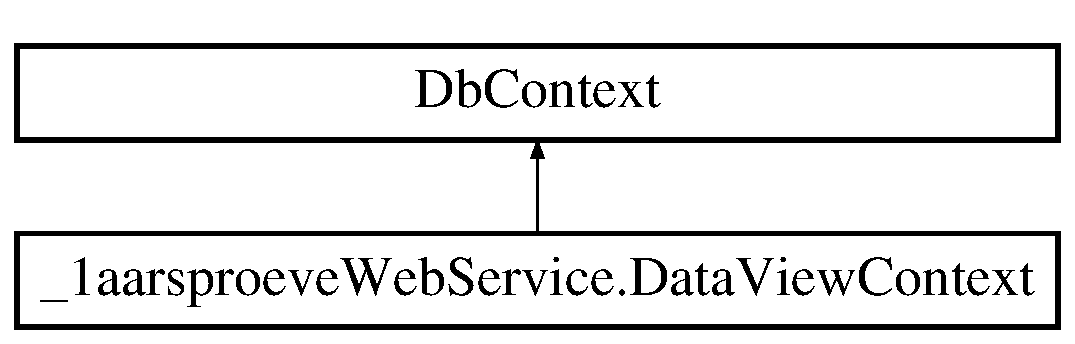
\includegraphics[height=2.000000cm]{class__1aarsproeve_web_service_1_1_data_view_context}
\end{center}
\end{figure}
\subsection*{Protected Member Functions}
\begin{DoxyCompactItemize}
\item 
\hypertarget{class__1aarsproeve_web_service_1_1_data_view_context_a419cff00a22f39825d2a46495b72027d}{}override void {\bfseries On\+Model\+Creating} (Db\+Model\+Builder model\+Builder)\label{class__1aarsproeve_web_service_1_1_data_view_context_a419cff00a22f39825d2a46495b72027d}

\end{DoxyCompactItemize}
\subsection*{Properties}
\begin{DoxyCompactItemize}
\item 
\hypertarget{class__1aarsproeve_web_service_1_1_data_view_context_a2c5de3890f5858a2abed788720b45091}{}virtual Db\+Set$<$ \hyperlink{class__1aarsproeve_web_service_1_1_ansatte_view}{Ansatte\+View} $>$ {\bfseries Ansatte\+Views}\hspace{0.3cm}{\ttfamily  \mbox{[}get, set\mbox{]}}\label{class__1aarsproeve_web_service_1_1_data_view_context_a2c5de3890f5858a2abed788720b45091}

\item 
\hypertarget{class__1aarsproeve_web_service_1_1_data_view_context_ac12b0249e2e6850381f2f3d2a2b1c4c0}{}virtual Db\+Set$<$ \hyperlink{class__1aarsproeve_web_service_1_1_hovedmenu_view}{Hovedmenu\+View} $>$ {\bfseries Hovedmenu\+Views}\hspace{0.3cm}{\ttfamily  \mbox{[}get, set\mbox{]}}\label{class__1aarsproeve_web_service_1_1_data_view_context_ac12b0249e2e6850381f2f3d2a2b1c4c0}

\item 
\hypertarget{class__1aarsproeve_web_service_1_1_data_view_context_a412d532b848e4264ca37fcc13772c284}{}virtual Db\+Set$<$ \hyperlink{class__1aarsproeve_web_service_1_1_vagtplan_view}{Vagtplan\+View} $>$ {\bfseries Vagtplan\+Views}\hspace{0.3cm}{\ttfamily  \mbox{[}get, set\mbox{]}}\label{class__1aarsproeve_web_service_1_1_data_view_context_a412d532b848e4264ca37fcc13772c284}

\end{DoxyCompactItemize}


The documentation for this class was generated from the following file\+:\begin{DoxyCompactItemize}
\item 
Documents/\+Git\+Hub/1-\/aarsproeve/1aarsproeve/1aarsproeve\+Web\+Service/Data\+View\+Context.\+cs\end{DoxyCompactItemize}

\hypertarget{class_w_s1aarsproeve_1_1_areas_1_1_help_page_1_1_model_descriptions_1_1_dictionary_model_description}{}\section{W\+S1aarsproeve.\+Areas.\+Help\+Page.\+Model\+Descriptions.\+Dictionary\+Model\+Description Class Reference}
\label{class_w_s1aarsproeve_1_1_areas_1_1_help_page_1_1_model_descriptions_1_1_dictionary_model_description}\index{W\+S1aarsproeve.\+Areas.\+Help\+Page.\+Model\+Descriptions.\+Dictionary\+Model\+Description@{W\+S1aarsproeve.\+Areas.\+Help\+Page.\+Model\+Descriptions.\+Dictionary\+Model\+Description}}
Inheritance diagram for W\+S1aarsproeve.\+Areas.\+Help\+Page.\+Model\+Descriptions.\+Dictionary\+Model\+Description\+:\begin{figure}[H]
\begin{center}
\leavevmode
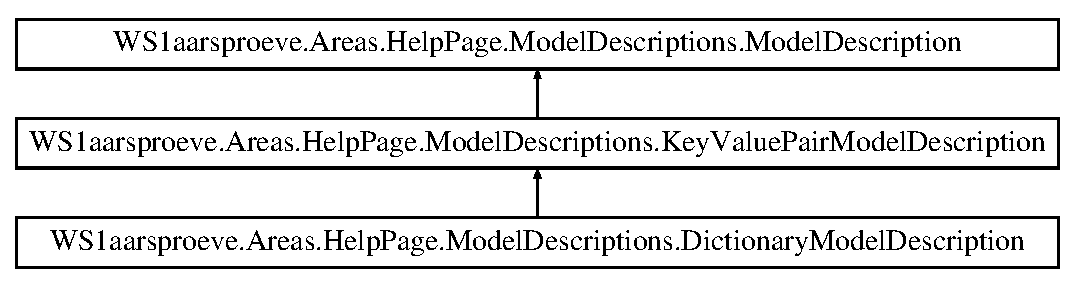
\includegraphics[height=3.000000cm]{class_w_s1aarsproeve_1_1_areas_1_1_help_page_1_1_model_descriptions_1_1_dictionary_model_description}
\end{center}
\end{figure}
\subsection*{Additional Inherited Members}


The documentation for this class was generated from the following file\+:\begin{DoxyCompactItemize}
\item 
Documents/\+Git\+Hub/1-\/aarsproeve/1aarsproeve/\+W\+S1aarsproeve/\+Areas/\+Help\+Page/\+Model\+Descriptions/Dictionary\+Model\+Description.\+cs\end{DoxyCompactItemize}

\hypertarget{class__1aarsproeve_web_service_1_1_areas_1_1_help_page_1_1_model_descriptions_1_1_dictionary_model_description}{}\section{\+\_\+1aarsproeve\+Web\+Service.\+Areas.\+Help\+Page.\+Model\+Descriptions.\+Dictionary\+Model\+Description Class Reference}
\label{class__1aarsproeve_web_service_1_1_areas_1_1_help_page_1_1_model_descriptions_1_1_dictionary_model_description}\index{\+\_\+1aarsproeve\+Web\+Service.\+Areas.\+Help\+Page.\+Model\+Descriptions.\+Dictionary\+Model\+Description@{\+\_\+1aarsproeve\+Web\+Service.\+Areas.\+Help\+Page.\+Model\+Descriptions.\+Dictionary\+Model\+Description}}
Inheritance diagram for \+\_\+1aarsproeve\+Web\+Service.\+Areas.\+Help\+Page.\+Model\+Descriptions.\+Dictionary\+Model\+Description\+:\begin{figure}[H]
\begin{center}
\leavevmode
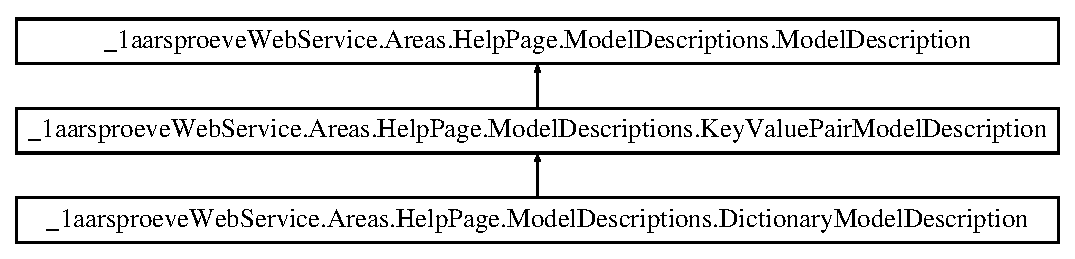
\includegraphics[height=3.000000cm]{class__1aarsproeve_web_service_1_1_areas_1_1_help_page_1_1_model_descriptions_1_1_dictionary_model_description}
\end{center}
\end{figure}
\subsection*{Additional Inherited Members}


The documentation for this class was generated from the following file\+:\begin{DoxyCompactItemize}
\item 
C\+:/\+Users/\+Daniel\+Winther/\+Documents/\+Git\+Hub/1-\/aarsproeve/1aarsproeve/1aarsproeve\+Web\+Service/\+Areas/\+Help\+Page/\+Model\+Descriptions/Dictionary\+Model\+Description.\+cs\end{DoxyCompactItemize}

\hypertarget{class_w_s1aarsproeve_1_1_areas_1_1_help_page_1_1_model_descriptions_1_1_enum_type_model_description}{}\section{W\+S1aarsproeve.\+Areas.\+Help\+Page.\+Model\+Descriptions.\+Enum\+Type\+Model\+Description Class Reference}
\label{class_w_s1aarsproeve_1_1_areas_1_1_help_page_1_1_model_descriptions_1_1_enum_type_model_description}\index{W\+S1aarsproeve.\+Areas.\+Help\+Page.\+Model\+Descriptions.\+Enum\+Type\+Model\+Description@{W\+S1aarsproeve.\+Areas.\+Help\+Page.\+Model\+Descriptions.\+Enum\+Type\+Model\+Description}}
Inheritance diagram for W\+S1aarsproeve.\+Areas.\+Help\+Page.\+Model\+Descriptions.\+Enum\+Type\+Model\+Description\+:\begin{figure}[H]
\begin{center}
\leavevmode
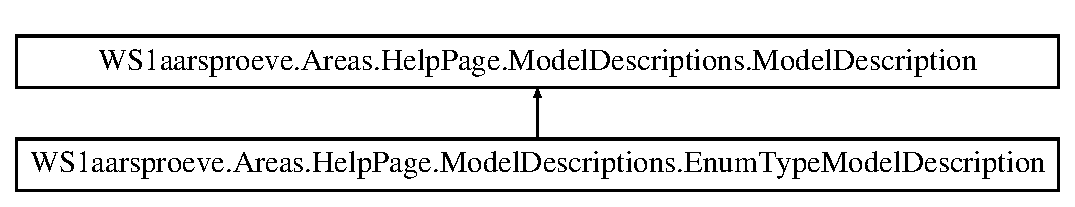
\includegraphics[height=2.000000cm]{class_w_s1aarsproeve_1_1_areas_1_1_help_page_1_1_model_descriptions_1_1_enum_type_model_description}
\end{center}
\end{figure}
\subsection*{Properties}
\begin{DoxyCompactItemize}
\item 
\hypertarget{class_w_s1aarsproeve_1_1_areas_1_1_help_page_1_1_model_descriptions_1_1_enum_type_model_description_a3cedd9b70da15d6fea894f81bca90e24}{}Collection$<$ \hyperlink{class_w_s1aarsproeve_1_1_areas_1_1_help_page_1_1_model_descriptions_1_1_enum_value_description}{Enum\+Value\+Description} $>$ {\bfseries Values}\hspace{0.3cm}{\ttfamily  \mbox{[}get\mbox{]}}\label{class_w_s1aarsproeve_1_1_areas_1_1_help_page_1_1_model_descriptions_1_1_enum_type_model_description_a3cedd9b70da15d6fea894f81bca90e24}

\end{DoxyCompactItemize}


The documentation for this class was generated from the following file\+:\begin{DoxyCompactItemize}
\item 
Documents/\+Git\+Hub/1-\/aarsproeve/1aarsproeve/\+W\+S1aarsproeve/\+Areas/\+Help\+Page/\+Model\+Descriptions/Enum\+Type\+Model\+Description.\+cs\end{DoxyCompactItemize}

\hypertarget{class__1aarsproeve_web_service_1_1_areas_1_1_help_page_1_1_model_descriptions_1_1_enum_type_model_description}{}\section{\+\_\+1aarsproeve\+Web\+Service.\+Areas.\+Help\+Page.\+Model\+Descriptions.\+Enum\+Type\+Model\+Description Class Reference}
\label{class__1aarsproeve_web_service_1_1_areas_1_1_help_page_1_1_model_descriptions_1_1_enum_type_model_description}\index{\+\_\+1aarsproeve\+Web\+Service.\+Areas.\+Help\+Page.\+Model\+Descriptions.\+Enum\+Type\+Model\+Description@{\+\_\+1aarsproeve\+Web\+Service.\+Areas.\+Help\+Page.\+Model\+Descriptions.\+Enum\+Type\+Model\+Description}}
Inheritance diagram for \+\_\+1aarsproeve\+Web\+Service.\+Areas.\+Help\+Page.\+Model\+Descriptions.\+Enum\+Type\+Model\+Description\+:\begin{figure}[H]
\begin{center}
\leavevmode
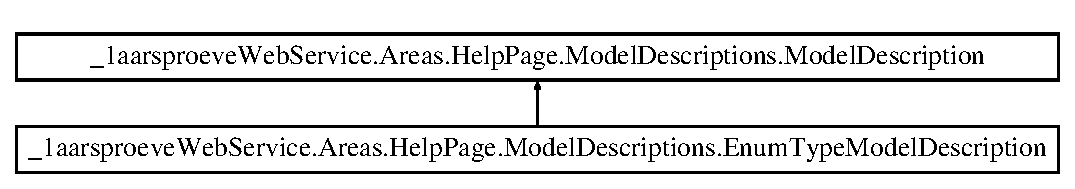
\includegraphics[height=2.000000cm]{class__1aarsproeve_web_service_1_1_areas_1_1_help_page_1_1_model_descriptions_1_1_enum_type_model_description}
\end{center}
\end{figure}
\subsection*{Properties}
\begin{DoxyCompactItemize}
\item 
\hypertarget{class__1aarsproeve_web_service_1_1_areas_1_1_help_page_1_1_model_descriptions_1_1_enum_type_model_description_a0d1a08eead95b9223e53b77770bc8703}{}Collection$<$ \hyperlink{class__1aarsproeve_web_service_1_1_areas_1_1_help_page_1_1_model_descriptions_1_1_enum_value_description}{Enum\+Value\+Description} $>$ {\bfseries Values}\hspace{0.3cm}{\ttfamily  \mbox{[}get\mbox{]}}\label{class__1aarsproeve_web_service_1_1_areas_1_1_help_page_1_1_model_descriptions_1_1_enum_type_model_description_a0d1a08eead95b9223e53b77770bc8703}

\end{DoxyCompactItemize}


The documentation for this class was generated from the following file\+:\begin{DoxyCompactItemize}
\item 
C\+:/\+Users/\+Daniel\+Winther/\+Documents/\+Git\+Hub/1-\/aarsproeve/1aarsproeve/1aarsproeve\+Web\+Service/\+Areas/\+Help\+Page/\+Model\+Descriptions/Enum\+Type\+Model\+Description.\+cs\end{DoxyCompactItemize}

\hypertarget{class_w_s1aarsproeve_1_1_areas_1_1_help_page_1_1_model_descriptions_1_1_enum_value_description}{}\section{W\+S1aarsproeve.\+Areas.\+Help\+Page.\+Model\+Descriptions.\+Enum\+Value\+Description Class Reference}
\label{class_w_s1aarsproeve_1_1_areas_1_1_help_page_1_1_model_descriptions_1_1_enum_value_description}\index{W\+S1aarsproeve.\+Areas.\+Help\+Page.\+Model\+Descriptions.\+Enum\+Value\+Description@{W\+S1aarsproeve.\+Areas.\+Help\+Page.\+Model\+Descriptions.\+Enum\+Value\+Description}}
\subsection*{Properties}
\begin{DoxyCompactItemize}
\item 
\hypertarget{class_w_s1aarsproeve_1_1_areas_1_1_help_page_1_1_model_descriptions_1_1_enum_value_description_a27958d14638e74e7f95caac4e70586a1}{}string {\bfseries Documentation}\hspace{0.3cm}{\ttfamily  \mbox{[}get, set\mbox{]}}\label{class_w_s1aarsproeve_1_1_areas_1_1_help_page_1_1_model_descriptions_1_1_enum_value_description_a27958d14638e74e7f95caac4e70586a1}

\item 
\hypertarget{class_w_s1aarsproeve_1_1_areas_1_1_help_page_1_1_model_descriptions_1_1_enum_value_description_a9c3304e6dc6b0e9885a612c523fd4c43}{}string {\bfseries Name}\hspace{0.3cm}{\ttfamily  \mbox{[}get, set\mbox{]}}\label{class_w_s1aarsproeve_1_1_areas_1_1_help_page_1_1_model_descriptions_1_1_enum_value_description_a9c3304e6dc6b0e9885a612c523fd4c43}

\item 
\hypertarget{class_w_s1aarsproeve_1_1_areas_1_1_help_page_1_1_model_descriptions_1_1_enum_value_description_a7329deaef785f63231e0c0b149c9a17c}{}string {\bfseries Value}\hspace{0.3cm}{\ttfamily  \mbox{[}get, set\mbox{]}}\label{class_w_s1aarsproeve_1_1_areas_1_1_help_page_1_1_model_descriptions_1_1_enum_value_description_a7329deaef785f63231e0c0b149c9a17c}

\end{DoxyCompactItemize}


The documentation for this class was generated from the following file\+:\begin{DoxyCompactItemize}
\item 
Documents/\+Git\+Hub/1-\/aarsproeve/1aarsproeve/\+W\+S1aarsproeve/\+Areas/\+Help\+Page/\+Model\+Descriptions/Enum\+Value\+Description.\+cs\end{DoxyCompactItemize}

\hypertarget{class__1aarsproeve_web_service_1_1_areas_1_1_help_page_1_1_model_descriptions_1_1_enum_value_description}{}\section{\+\_\+1aarsproeve\+Web\+Service.\+Areas.\+Help\+Page.\+Model\+Descriptions.\+Enum\+Value\+Description Class Reference}
\label{class__1aarsproeve_web_service_1_1_areas_1_1_help_page_1_1_model_descriptions_1_1_enum_value_description}\index{\+\_\+1aarsproeve\+Web\+Service.\+Areas.\+Help\+Page.\+Model\+Descriptions.\+Enum\+Value\+Description@{\+\_\+1aarsproeve\+Web\+Service.\+Areas.\+Help\+Page.\+Model\+Descriptions.\+Enum\+Value\+Description}}
\subsection*{Properties}
\begin{DoxyCompactItemize}
\item 
\hypertarget{class__1aarsproeve_web_service_1_1_areas_1_1_help_page_1_1_model_descriptions_1_1_enum_value_description_a8b2b1e0baf970953a104b1c468a68c61}{}string {\bfseries Documentation}\hspace{0.3cm}{\ttfamily  \mbox{[}get, set\mbox{]}}\label{class__1aarsproeve_web_service_1_1_areas_1_1_help_page_1_1_model_descriptions_1_1_enum_value_description_a8b2b1e0baf970953a104b1c468a68c61}

\item 
\hypertarget{class__1aarsproeve_web_service_1_1_areas_1_1_help_page_1_1_model_descriptions_1_1_enum_value_description_a7d3d2652afe86ecef65fa066bd7a233b}{}string {\bfseries Name}\hspace{0.3cm}{\ttfamily  \mbox{[}get, set\mbox{]}}\label{class__1aarsproeve_web_service_1_1_areas_1_1_help_page_1_1_model_descriptions_1_1_enum_value_description_a7d3d2652afe86ecef65fa066bd7a233b}

\item 
\hypertarget{class__1aarsproeve_web_service_1_1_areas_1_1_help_page_1_1_model_descriptions_1_1_enum_value_description_a0670b18ee3d0ffe91340b5bc62e1b21a}{}string {\bfseries Value}\hspace{0.3cm}{\ttfamily  \mbox{[}get, set\mbox{]}}\label{class__1aarsproeve_web_service_1_1_areas_1_1_help_page_1_1_model_descriptions_1_1_enum_value_description_a0670b18ee3d0ffe91340b5bc62e1b21a}

\end{DoxyCompactItemize}


The documentation for this class was generated from the following file\+:\begin{DoxyCompactItemize}
\item 
Documents/\+Git\+Hub/1-\/aarsproeve/1aarsproeve/1aarsproeve\+Web\+Service/\+Areas/\+Help\+Page/\+Model\+Descriptions/Enum\+Value\+Description.\+cs\end{DoxyCompactItemize}

\hypertarget{class_w_s1aarsproeve_1_1_filter_config}{}\section{W\+S1aarsproeve.\+Filter\+Config Class Reference}
\label{class_w_s1aarsproeve_1_1_filter_config}\index{W\+S1aarsproeve.\+Filter\+Config@{W\+S1aarsproeve.\+Filter\+Config}}
\subsection*{Static Public Member Functions}
\begin{DoxyCompactItemize}
\item 
\hypertarget{class_w_s1aarsproeve_1_1_filter_config_a79fefc6789d5950c86ccd0fba0a40cb3}{}static void {\bfseries Register\+Global\+Filters} (Global\+Filter\+Collection filters)\label{class_w_s1aarsproeve_1_1_filter_config_a79fefc6789d5950c86ccd0fba0a40cb3}

\end{DoxyCompactItemize}


The documentation for this class was generated from the following file\+:\begin{DoxyCompactItemize}
\item 
Documents/\+Git\+Hub/1-\/aarsproeve/1aarsproeve/\+W\+S1aarsproeve/\+App\+\_\+\+Start/Filter\+Config.\+cs\end{DoxyCompactItemize}

\hypertarget{class__1aarsproeve_web_service_1_1_filter_config}{}\section{\+\_\+1aarsproeve\+Web\+Service.\+Filter\+Config Class Reference}
\label{class__1aarsproeve_web_service_1_1_filter_config}\index{\+\_\+1aarsproeve\+Web\+Service.\+Filter\+Config@{\+\_\+1aarsproeve\+Web\+Service.\+Filter\+Config}}
\subsection*{Static Public Member Functions}
\begin{DoxyCompactItemize}
\item 
\hypertarget{class__1aarsproeve_web_service_1_1_filter_config_aa408c602cd6d9244e1299d9c2ab9566e}{}static void {\bfseries Register\+Global\+Filters} (Global\+Filter\+Collection filters)\label{class__1aarsproeve_web_service_1_1_filter_config_aa408c602cd6d9244e1299d9c2ab9566e}

\end{DoxyCompactItemize}


The documentation for this class was generated from the following file\+:\begin{DoxyCompactItemize}
\item 
Documents/\+Git\+Hub/1-\/aarsproeve/1aarsproeve/1aarsproeve\+Web\+Service/\+App\+\_\+\+Start/Filter\+Config.\+cs\end{DoxyCompactItemize}

\hypertarget{class__1aarsproeve_1_1_strategy_1_1_frie_vagter}{}\section{\+\_\+1aarsproeve.\+Strategy.\+Frie\+Vagter Class Reference}
\label{class__1aarsproeve_1_1_strategy_1_1_frie_vagter}\index{\+\_\+1aarsproeve.\+Strategy.\+Frie\+Vagter@{\+\_\+1aarsproeve.\+Strategy.\+Frie\+Vagter}}


\hyperlink{namespace__1aarsproeve_1_1_strategy}{Strategy} klasse der implmenterer \hyperlink{interface__1aarsproeve_1_1_strategy_1_1_i_vagt_sort}{I\+Vagt\+Sort} interfacet  


Inheritance diagram for \+\_\+1aarsproeve.\+Strategy.\+Frie\+Vagter\+:\begin{figure}[H]
\begin{center}
\leavevmode
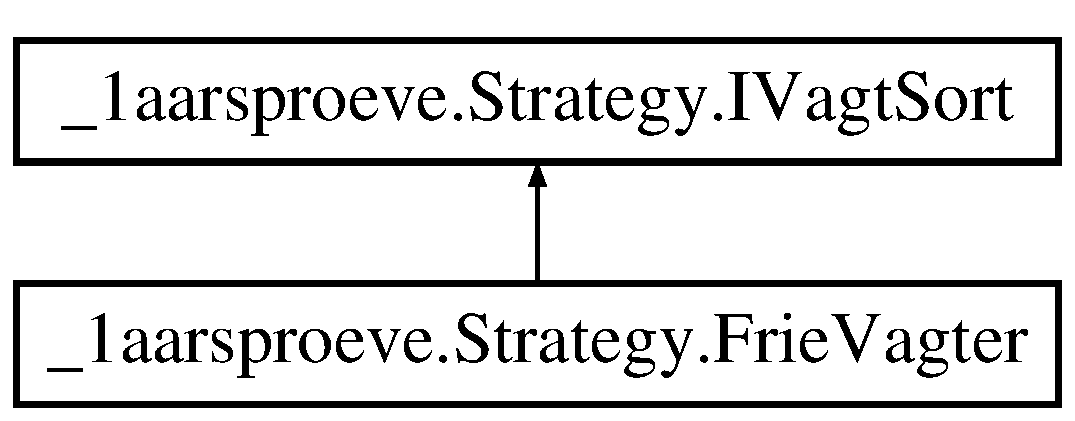
\includegraphics[height=2.000000cm]{class__1aarsproeve_1_1_strategy_1_1_frie_vagter}
\end{center}
\end{figure}
\subsection*{Public Member Functions}
\begin{DoxyCompactItemize}
\item 
async void \hyperlink{class__1aarsproeve_1_1_strategy_1_1_frie_vagter_ae1a30073de8aceb36378f7e7f2bd1e66}{Sort} (Observable\+Collection$<$ Observable\+Collection$<$ \hyperlink{class__1aarsproeve_1_1_model_1_1_vagtplan_view}{Vagtplan\+View} $>$$>$ vagt\+Collection, int ugenummer)
\begin{DoxyCompactList}\small\item\em Sorterer vagterne udfra Mine vagter \end{DoxyCompactList}\end{DoxyCompactItemize}


\subsection{Detailed Description}
\hyperlink{namespace__1aarsproeve_1_1_strategy}{Strategy} klasse der implmenterer \hyperlink{interface__1aarsproeve_1_1_strategy_1_1_i_vagt_sort}{I\+Vagt\+Sort} interfacet 



\subsection{Member Function Documentation}
\hypertarget{class__1aarsproeve_1_1_strategy_1_1_frie_vagter_ae1a30073de8aceb36378f7e7f2bd1e66}{}\index{\+\_\+1aarsproeve\+::\+Strategy\+::\+Frie\+Vagter@{\+\_\+1aarsproeve\+::\+Strategy\+::\+Frie\+Vagter}!Sort@{Sort}}
\index{Sort@{Sort}!\+\_\+1aarsproeve\+::\+Strategy\+::\+Frie\+Vagter@{\+\_\+1aarsproeve\+::\+Strategy\+::\+Frie\+Vagter}}
\subsubsection[{Sort}]{\setlength{\rightskip}{0pt plus 5cm}async void \+\_\+1aarsproeve.\+Strategy.\+Frie\+Vagter.\+Sort (
\begin{DoxyParamCaption}
\item[{Observable\+Collection$<$ Observable\+Collection$<$ {\bf Vagtplan\+View} $>$$>$}]{vagt\+Collection, }
\item[{int}]{ugenummer}
\end{DoxyParamCaption}
)}\label{class__1aarsproeve_1_1_strategy_1_1_frie_vagter_ae1a30073de8aceb36378f7e7f2bd1e66}


Sorterer vagterne udfra Mine vagter 


\begin{DoxyParams}{Parameters}
{\em vagt\+Collection} & Angiver hvilken collection der skal sorteres\\
\hline
{\em ugenummer} & Angiver for hvilken uge vagterne skal vises i\\
\hline
\end{DoxyParams}


Implements \hyperlink{interface__1aarsproeve_1_1_strategy_1_1_i_vagt_sort}{\+\_\+1aarsproeve.\+Strategy.\+I\+Vagt\+Sort}.



The documentation for this class was generated from the following file\+:\begin{DoxyCompactItemize}
\item 
Documents/\+Git\+Hub/1-\/aarsproeve/1aarsproeve/1aarsproeve/\+Strategy/Frie\+Vagter.\+cs\end{DoxyCompactItemize}

\hypertarget{class__1aarsproeve_1_1_model_1_1_generisk_singleton}{}\section{\+\_\+1aarsproeve.\+Model.\+Generisk\+Singleton$<$ T $>$ Class Template Reference}
\label{class__1aarsproeve_1_1_model_1_1_generisk_singleton}\index{\+\_\+1aarsproeve.\+Model.\+Generisk\+Singleton$<$ T $>$@{\+\_\+1aarsproeve.\+Model.\+Generisk\+Singleton$<$ T $>$}}


Generisk Singleton Klasse  


\subsection*{Public Member Functions}
\begin{DoxyCompactItemize}
\item 
void \hyperlink{class__1aarsproeve_1_1_model_1_1_generisk_singleton_a600d0c0ce520544d7037730f6c857aaa}{Load\+Generisk} ()
\begin{DoxyCompactList}\small\item\em Generisk load-\/metode \end{DoxyCompactList}\end{DoxyCompactItemize}
\subsection*{Static Public Member Functions}
\begin{DoxyCompactItemize}
\item 
static \hyperlink{class__1aarsproeve_1_1_model_1_1_generisk_singleton}{Generisk\+Singleton}$<$ T $>$ \hyperlink{class__1aarsproeve_1_1_model_1_1_generisk_singleton_a68d5e62e7d199df6c63011a4ac6e43b6}{Instance} ()
\begin{DoxyCompactList}\small\item\em Instance metoden der definere singleton \end{DoxyCompactList}\end{DoxyCompactItemize}
\subsection*{Properties}
\begin{DoxyCompactItemize}
\item 
Observable\+Collection$<$ T $>$ \hyperlink{class__1aarsproeve_1_1_model_1_1_generisk_singleton_a350a2fb273daada34ad4fab80105b543}{Collection}\hspace{0.3cm}{\ttfamily  \mbox{[}get, set\mbox{]}}
\begin{DoxyCompactList}\small\item\em Collection Property \end{DoxyCompactList}\end{DoxyCompactItemize}


\subsection{Detailed Description}
Generisk Singleton Klasse 


\begin{DoxyTemplParams}{Template Parameters}
{\em T} & Generisk type\\
\hline
\end{DoxyTemplParams}


\subsection{Member Function Documentation}
\hypertarget{class__1aarsproeve_1_1_model_1_1_generisk_singleton_a68d5e62e7d199df6c63011a4ac6e43b6}{}\index{\+\_\+1aarsproeve\+::\+Model\+::\+Generisk\+Singleton@{\+\_\+1aarsproeve\+::\+Model\+::\+Generisk\+Singleton}!Instance@{Instance}}
\index{Instance@{Instance}!\+\_\+1aarsproeve\+::\+Model\+::\+Generisk\+Singleton@{\+\_\+1aarsproeve\+::\+Model\+::\+Generisk\+Singleton}}
\subsubsection[{Instance}]{\setlength{\rightskip}{0pt plus 5cm}static {\bf Generisk\+Singleton}$<$T$>$ {\bf \+\_\+1aarsproeve.\+Model.\+Generisk\+Singleton}$<$ T $>$.Instance (
\begin{DoxyParamCaption}
{}
\end{DoxyParamCaption}
)\hspace{0.3cm}{\ttfamily [static]}}\label{class__1aarsproeve_1_1_model_1_1_generisk_singleton_a68d5e62e7d199df6c63011a4ac6e43b6}


Instance metoden der definere singleton 

\begin{DoxyReturn}{Returns}
\+\_\+instance som er et objekt af \hyperlink{class__1aarsproeve_1_1_model_1_1_generisk_singleton}{Generisk\+Singleton} 
\end{DoxyReturn}
\hypertarget{class__1aarsproeve_1_1_model_1_1_generisk_singleton_a600d0c0ce520544d7037730f6c857aaa}{}\index{\+\_\+1aarsproeve\+::\+Model\+::\+Generisk\+Singleton@{\+\_\+1aarsproeve\+::\+Model\+::\+Generisk\+Singleton}!Load\+Generisk@{Load\+Generisk}}
\index{Load\+Generisk@{Load\+Generisk}!\+\_\+1aarsproeve\+::\+Model\+::\+Generisk\+Singleton@{\+\_\+1aarsproeve\+::\+Model\+::\+Generisk\+Singleton}}
\subsubsection[{Load\+Generisk}]{\setlength{\rightskip}{0pt plus 5cm}void {\bf \+\_\+1aarsproeve.\+Model.\+Generisk\+Singleton}$<$ T $>$.Load\+Generisk (
\begin{DoxyParamCaption}
{}
\end{DoxyParamCaption}
)}\label{class__1aarsproeve_1_1_model_1_1_generisk_singleton_a600d0c0ce520544d7037730f6c857aaa}


Generisk load-\/metode 



\subsection{Property Documentation}
\hypertarget{class__1aarsproeve_1_1_model_1_1_generisk_singleton_a350a2fb273daada34ad4fab80105b543}{}\index{\+\_\+1aarsproeve\+::\+Model\+::\+Generisk\+Singleton@{\+\_\+1aarsproeve\+::\+Model\+::\+Generisk\+Singleton}!Collection@{Collection}}
\index{Collection@{Collection}!\+\_\+1aarsproeve\+::\+Model\+::\+Generisk\+Singleton@{\+\_\+1aarsproeve\+::\+Model\+::\+Generisk\+Singleton}}
\subsubsection[{Collection}]{\setlength{\rightskip}{0pt plus 5cm}Observable\+Collection$<$T$>$ {\bf \+\_\+1aarsproeve.\+Model.\+Generisk\+Singleton}$<$ T $>$.Collection\hspace{0.3cm}{\ttfamily [get]}, {\ttfamily [set]}}\label{class__1aarsproeve_1_1_model_1_1_generisk_singleton_a350a2fb273daada34ad4fab80105b543}


Collection Property 



The documentation for this class was generated from the following file\+:\begin{DoxyCompactItemize}
\item 
Documents/\+Git\+Hub/1-\/aarsproeve/1aarsproeve/1aarsproeve/\+Model/Generisk\+Singleton.\+cs\end{DoxyCompactItemize}

\hypertarget{class_w_s1aarsproeve_1_1_areas_1_1_help_page_1_1_controllers_1_1_help_controller}{}\section{W\+S1aarsproeve.\+Areas.\+Help\+Page.\+Controllers.\+Help\+Controller Class Reference}
\label{class_w_s1aarsproeve_1_1_areas_1_1_help_page_1_1_controllers_1_1_help_controller}\index{W\+S1aarsproeve.\+Areas.\+Help\+Page.\+Controllers.\+Help\+Controller@{W\+S1aarsproeve.\+Areas.\+Help\+Page.\+Controllers.\+Help\+Controller}}


The controller that will handle requests for the help page.  


Inheritance diagram for W\+S1aarsproeve.\+Areas.\+Help\+Page.\+Controllers.\+Help\+Controller\+:\begin{figure}[H]
\begin{center}
\leavevmode
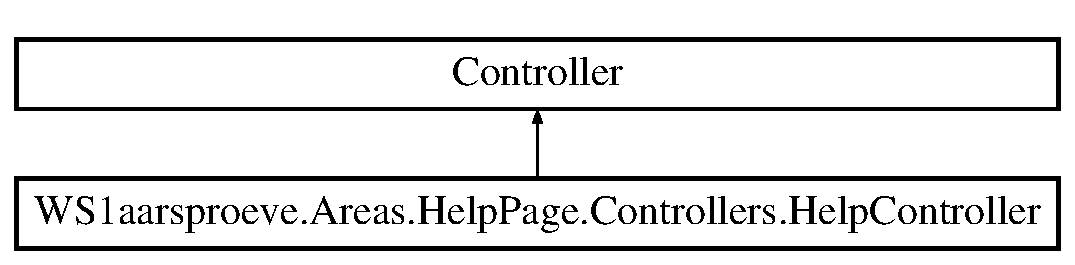
\includegraphics[height=2.000000cm]{class_w_s1aarsproeve_1_1_areas_1_1_help_page_1_1_controllers_1_1_help_controller}
\end{center}
\end{figure}
\subsection*{Public Member Functions}
\begin{DoxyCompactItemize}
\item 
\hypertarget{class_w_s1aarsproeve_1_1_areas_1_1_help_page_1_1_controllers_1_1_help_controller_a1e5fef2ae84c90a23b4751f3c1bd54cc}{}{\bfseries Help\+Controller} (Http\+Configuration config)\label{class_w_s1aarsproeve_1_1_areas_1_1_help_page_1_1_controllers_1_1_help_controller_a1e5fef2ae84c90a23b4751f3c1bd54cc}

\item 
\hypertarget{class_w_s1aarsproeve_1_1_areas_1_1_help_page_1_1_controllers_1_1_help_controller_a36177bd3bea04ea645601ba789c81f4d}{}Action\+Result {\bfseries Index} ()\label{class_w_s1aarsproeve_1_1_areas_1_1_help_page_1_1_controllers_1_1_help_controller_a36177bd3bea04ea645601ba789c81f4d}

\item 
\hypertarget{class_w_s1aarsproeve_1_1_areas_1_1_help_page_1_1_controllers_1_1_help_controller_aaa766b1d1e1d737faba2d707be97de05}{}Action\+Result {\bfseries Api} (string api\+Id)\label{class_w_s1aarsproeve_1_1_areas_1_1_help_page_1_1_controllers_1_1_help_controller_aaa766b1d1e1d737faba2d707be97de05}

\item 
\hypertarget{class_w_s1aarsproeve_1_1_areas_1_1_help_page_1_1_controllers_1_1_help_controller_ad0816892041880bd4caefd7aa2e306d0}{}Action\+Result {\bfseries Resource\+Model} (string model\+Name)\label{class_w_s1aarsproeve_1_1_areas_1_1_help_page_1_1_controllers_1_1_help_controller_ad0816892041880bd4caefd7aa2e306d0}

\end{DoxyCompactItemize}
\subsection*{Properties}
\begin{DoxyCompactItemize}
\item 
\hypertarget{class_w_s1aarsproeve_1_1_areas_1_1_help_page_1_1_controllers_1_1_help_controller_a67810b47daa31e488bb0ab5d5038013d}{}Http\+Configuration {\bfseries Configuration}\hspace{0.3cm}{\ttfamily  \mbox{[}get\mbox{]}}\label{class_w_s1aarsproeve_1_1_areas_1_1_help_page_1_1_controllers_1_1_help_controller_a67810b47daa31e488bb0ab5d5038013d}

\end{DoxyCompactItemize}


\subsection{Detailed Description}
The controller that will handle requests for the help page. 



The documentation for this class was generated from the following file\+:\begin{DoxyCompactItemize}
\item 
Documents/\+Git\+Hub/1-\/aarsproeve/1aarsproeve/\+W\+S1aarsproeve/\+Areas/\+Help\+Page/\+Controllers/Help\+Controller.\+cs\end{DoxyCompactItemize}

\hypertarget{class__1aarsproeve_web_service_1_1_areas_1_1_help_page_1_1_controllers_1_1_help_controller}{}\section{\+\_\+1aarsproeve\+Web\+Service.\+Areas.\+Help\+Page.\+Controllers.\+Help\+Controller Class Reference}
\label{class__1aarsproeve_web_service_1_1_areas_1_1_help_page_1_1_controllers_1_1_help_controller}\index{\+\_\+1aarsproeve\+Web\+Service.\+Areas.\+Help\+Page.\+Controllers.\+Help\+Controller@{\+\_\+1aarsproeve\+Web\+Service.\+Areas.\+Help\+Page.\+Controllers.\+Help\+Controller}}


The controller that will handle requests for the help page.  


Inheritance diagram for \+\_\+1aarsproeve\+Web\+Service.\+Areas.\+Help\+Page.\+Controllers.\+Help\+Controller\+:\begin{figure}[H]
\begin{center}
\leavevmode
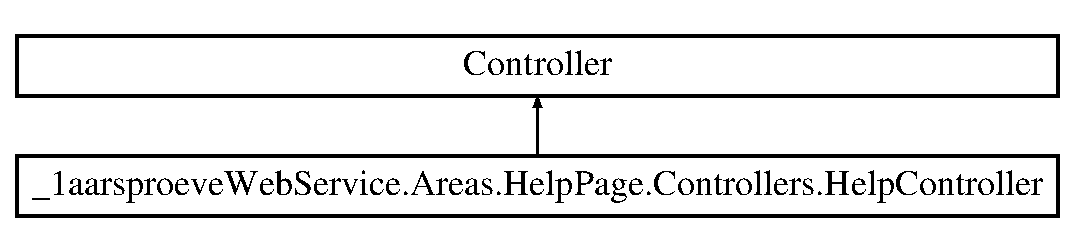
\includegraphics[height=2.000000cm]{class__1aarsproeve_web_service_1_1_areas_1_1_help_page_1_1_controllers_1_1_help_controller}
\end{center}
\end{figure}
\subsection*{Public Member Functions}
\begin{DoxyCompactItemize}
\item 
\hypertarget{class__1aarsproeve_web_service_1_1_areas_1_1_help_page_1_1_controllers_1_1_help_controller_ac5863469ead4f269ca923864b1b000bb}{}{\bfseries Help\+Controller} (Http\+Configuration config)\label{class__1aarsproeve_web_service_1_1_areas_1_1_help_page_1_1_controllers_1_1_help_controller_ac5863469ead4f269ca923864b1b000bb}

\item 
\hypertarget{class__1aarsproeve_web_service_1_1_areas_1_1_help_page_1_1_controllers_1_1_help_controller_ac8ab14f8de06e3b728040556b86976bb}{}Action\+Result {\bfseries Index} ()\label{class__1aarsproeve_web_service_1_1_areas_1_1_help_page_1_1_controllers_1_1_help_controller_ac8ab14f8de06e3b728040556b86976bb}

\item 
\hypertarget{class__1aarsproeve_web_service_1_1_areas_1_1_help_page_1_1_controllers_1_1_help_controller_aedb2d9f385044bd702dde25cd83ef505}{}Action\+Result {\bfseries Api} (string api\+Id)\label{class__1aarsproeve_web_service_1_1_areas_1_1_help_page_1_1_controllers_1_1_help_controller_aedb2d9f385044bd702dde25cd83ef505}

\item 
\hypertarget{class__1aarsproeve_web_service_1_1_areas_1_1_help_page_1_1_controllers_1_1_help_controller_a0d6027c97d0dfaf55e3399a8ec8625b7}{}Action\+Result {\bfseries Resource\+Model} (string model\+Name)\label{class__1aarsproeve_web_service_1_1_areas_1_1_help_page_1_1_controllers_1_1_help_controller_a0d6027c97d0dfaf55e3399a8ec8625b7}

\end{DoxyCompactItemize}
\subsection*{Properties}
\begin{DoxyCompactItemize}
\item 
\hypertarget{class__1aarsproeve_web_service_1_1_areas_1_1_help_page_1_1_controllers_1_1_help_controller_ae617e8e48348cf6dd582b758ee6cef66}{}Http\+Configuration {\bfseries Configuration}\hspace{0.3cm}{\ttfamily  \mbox{[}get\mbox{]}}\label{class__1aarsproeve_web_service_1_1_areas_1_1_help_page_1_1_controllers_1_1_help_controller_ae617e8e48348cf6dd582b758ee6cef66}

\end{DoxyCompactItemize}


\subsection{Detailed Description}
The controller that will handle requests for the help page. 



The documentation for this class was generated from the following file\+:\begin{DoxyCompactItemize}
\item 
C\+:/\+Users/\+Daniel\+Winther/\+Documents/\+Git\+Hub/1-\/aarsproeve/1aarsproeve/1aarsproeve\+Web\+Service/\+Areas/\+Help\+Page/\+Controllers/Help\+Controller.\+cs\end{DoxyCompactItemize}

\hypertarget{class__1aarsproeve_web_service_1_1_areas_1_1_help_page_1_1_models_1_1_help_page_api_model}{}\section{\+\_\+1aarsproeve\+Web\+Service.\+Areas.\+Help\+Page.\+Models.\+Help\+Page\+Api\+Model Class Reference}
\label{class__1aarsproeve_web_service_1_1_areas_1_1_help_page_1_1_models_1_1_help_page_api_model}\index{\+\_\+1aarsproeve\+Web\+Service.\+Areas.\+Help\+Page.\+Models.\+Help\+Page\+Api\+Model@{\+\_\+1aarsproeve\+Web\+Service.\+Areas.\+Help\+Page.\+Models.\+Help\+Page\+Api\+Model}}


The model that represents an A\+P\+I displayed on the help page.  


\subsection*{Public Member Functions}
\begin{DoxyCompactItemize}
\item 
\hyperlink{class__1aarsproeve_web_service_1_1_areas_1_1_help_page_1_1_models_1_1_help_page_api_model_aea81d3b4b0294cd9753efb03c91bf2eb}{Help\+Page\+Api\+Model} ()
\begin{DoxyCompactList}\small\item\em Initializes a new instance of the \hyperlink{class__1aarsproeve_web_service_1_1_areas_1_1_help_page_1_1_models_1_1_help_page_api_model}{Help\+Page\+Api\+Model} class. \end{DoxyCompactList}\end{DoxyCompactItemize}
\subsection*{Properties}
\begin{DoxyCompactItemize}
\item 
Api\+Description \hyperlink{class__1aarsproeve_web_service_1_1_areas_1_1_help_page_1_1_models_1_1_help_page_api_model_a8b1d233d46646da325139313fe77cedc}{Api\+Description}\hspace{0.3cm}{\ttfamily  \mbox{[}get, set\mbox{]}}
\begin{DoxyCompactList}\small\item\em Gets or sets the \hyperlink{class__1aarsproeve_web_service_1_1_areas_1_1_help_page_1_1_models_1_1_help_page_api_model_a8b1d233d46646da325139313fe77cedc}{Api\+Description} that describes the A\+P\+I. \end{DoxyCompactList}\item 
Collection$<$ \hyperlink{class__1aarsproeve_web_service_1_1_areas_1_1_help_page_1_1_model_descriptions_1_1_parameter_description}{Parameter\+Description} $>$ \hyperlink{class__1aarsproeve_web_service_1_1_areas_1_1_help_page_1_1_models_1_1_help_page_api_model_a13910e263edc19222bbb60615d1f80be}{Uri\+Parameters}\hspace{0.3cm}{\ttfamily  \mbox{[}get\mbox{]}}
\begin{DoxyCompactList}\small\item\em Gets or sets the Parameter\+Description collection that describes the U\+R\+I parameters for the A\+P\+I. \end{DoxyCompactList}\item 
string \hyperlink{class__1aarsproeve_web_service_1_1_areas_1_1_help_page_1_1_models_1_1_help_page_api_model_a7c6ab7ddf1586125e6de402d850fddab}{Request\+Documentation}\hspace{0.3cm}{\ttfamily  \mbox{[}get, set\mbox{]}}
\begin{DoxyCompactList}\small\item\em Gets or sets the documentation for the request. \end{DoxyCompactList}\item 
\hyperlink{class__1aarsproeve_web_service_1_1_areas_1_1_help_page_1_1_model_descriptions_1_1_model_description}{Model\+Description} \hyperlink{class__1aarsproeve_web_service_1_1_areas_1_1_help_page_1_1_models_1_1_help_page_api_model_ab70ab5430b41f8c40c1ff4bb5aec3eca}{Request\+Model\+Description}\hspace{0.3cm}{\ttfamily  \mbox{[}get, set\mbox{]}}
\begin{DoxyCompactList}\small\item\em Gets or sets the Model\+Description that describes the request body. \end{DoxyCompactList}\item 
I\+List$<$ \hyperlink{class__1aarsproeve_web_service_1_1_areas_1_1_help_page_1_1_model_descriptions_1_1_parameter_description}{Parameter\+Description} $>$ \hyperlink{class__1aarsproeve_web_service_1_1_areas_1_1_help_page_1_1_models_1_1_help_page_api_model_a01d824c4a2e89f5c4464fc1a077361a6}{Request\+Body\+Parameters}\hspace{0.3cm}{\ttfamily  \mbox{[}get\mbox{]}}
\begin{DoxyCompactList}\small\item\em Gets the request body parameter descriptions. \end{DoxyCompactList}\item 
\hyperlink{class__1aarsproeve_web_service_1_1_areas_1_1_help_page_1_1_model_descriptions_1_1_model_description}{Model\+Description} \hyperlink{class__1aarsproeve_web_service_1_1_areas_1_1_help_page_1_1_models_1_1_help_page_api_model_a190780aa4262f4e6da85944b57e57307}{Resource\+Description}\hspace{0.3cm}{\ttfamily  \mbox{[}get, set\mbox{]}}
\begin{DoxyCompactList}\small\item\em Gets or sets the Model\+Description that describes the resource. \end{DoxyCompactList}\item 
I\+List$<$ \hyperlink{class__1aarsproeve_web_service_1_1_areas_1_1_help_page_1_1_model_descriptions_1_1_parameter_description}{Parameter\+Description} $>$ \hyperlink{class__1aarsproeve_web_service_1_1_areas_1_1_help_page_1_1_models_1_1_help_page_api_model_a9ab05000ce11c2ab4d69f190f2177239}{Resource\+Properties}\hspace{0.3cm}{\ttfamily  \mbox{[}get\mbox{]}}
\begin{DoxyCompactList}\small\item\em Gets the resource property descriptions. \end{DoxyCompactList}\item 
I\+Dictionary$<$ Media\+Type\+Header\+Value, object $>$ \hyperlink{class__1aarsproeve_web_service_1_1_areas_1_1_help_page_1_1_models_1_1_help_page_api_model_a28948b3477b00b650df4df27d9a1b866}{Sample\+Requests}\hspace{0.3cm}{\ttfamily  \mbox{[}get\mbox{]}}
\begin{DoxyCompactList}\small\item\em Gets the sample requests associated with the A\+P\+I. \end{DoxyCompactList}\item 
I\+Dictionary$<$ Media\+Type\+Header\+Value, object $>$ \hyperlink{class__1aarsproeve_web_service_1_1_areas_1_1_help_page_1_1_models_1_1_help_page_api_model_aa2176c7fd5b4e47329d2cecee146fdaa}{Sample\+Responses}\hspace{0.3cm}{\ttfamily  \mbox{[}get\mbox{]}}
\begin{DoxyCompactList}\small\item\em Gets the sample responses associated with the A\+P\+I. \end{DoxyCompactList}\item 
Collection$<$ string $>$ \hyperlink{class__1aarsproeve_web_service_1_1_areas_1_1_help_page_1_1_models_1_1_help_page_api_model_a89a4a8ab5f162a7feca59255edef5e50}{Error\+Messages}\hspace{0.3cm}{\ttfamily  \mbox{[}get\mbox{]}}
\begin{DoxyCompactList}\small\item\em Gets the error messages associated with this model. \end{DoxyCompactList}\end{DoxyCompactItemize}


\subsection{Detailed Description}
The model that represents an A\+P\+I displayed on the help page. 



\subsection{Constructor \& Destructor Documentation}
\hypertarget{class__1aarsproeve_web_service_1_1_areas_1_1_help_page_1_1_models_1_1_help_page_api_model_aea81d3b4b0294cd9753efb03c91bf2eb}{}\index{\+\_\+1aarsproeve\+Web\+Service\+::\+Areas\+::\+Help\+Page\+::\+Models\+::\+Help\+Page\+Api\+Model@{\+\_\+1aarsproeve\+Web\+Service\+::\+Areas\+::\+Help\+Page\+::\+Models\+::\+Help\+Page\+Api\+Model}!Help\+Page\+Api\+Model@{Help\+Page\+Api\+Model}}
\index{Help\+Page\+Api\+Model@{Help\+Page\+Api\+Model}!\+\_\+1aarsproeve\+Web\+Service\+::\+Areas\+::\+Help\+Page\+::\+Models\+::\+Help\+Page\+Api\+Model@{\+\_\+1aarsproeve\+Web\+Service\+::\+Areas\+::\+Help\+Page\+::\+Models\+::\+Help\+Page\+Api\+Model}}
\subsubsection[{Help\+Page\+Api\+Model}]{\setlength{\rightskip}{0pt plus 5cm}\+\_\+1aarsproeve\+Web\+Service.\+Areas.\+Help\+Page.\+Models.\+Help\+Page\+Api\+Model.\+Help\+Page\+Api\+Model (
\begin{DoxyParamCaption}
{}
\end{DoxyParamCaption}
)\hspace{0.3cm}{\ttfamily [inline]}}\label{class__1aarsproeve_web_service_1_1_areas_1_1_help_page_1_1_models_1_1_help_page_api_model_aea81d3b4b0294cd9753efb03c91bf2eb}


Initializes a new instance of the \hyperlink{class__1aarsproeve_web_service_1_1_areas_1_1_help_page_1_1_models_1_1_help_page_api_model}{Help\+Page\+Api\+Model} class. 



\subsection{Property Documentation}
\hypertarget{class__1aarsproeve_web_service_1_1_areas_1_1_help_page_1_1_models_1_1_help_page_api_model_a8b1d233d46646da325139313fe77cedc}{}\index{\+\_\+1aarsproeve\+Web\+Service\+::\+Areas\+::\+Help\+Page\+::\+Models\+::\+Help\+Page\+Api\+Model@{\+\_\+1aarsproeve\+Web\+Service\+::\+Areas\+::\+Help\+Page\+::\+Models\+::\+Help\+Page\+Api\+Model}!Api\+Description@{Api\+Description}}
\index{Api\+Description@{Api\+Description}!\+\_\+1aarsproeve\+Web\+Service\+::\+Areas\+::\+Help\+Page\+::\+Models\+::\+Help\+Page\+Api\+Model@{\+\_\+1aarsproeve\+Web\+Service\+::\+Areas\+::\+Help\+Page\+::\+Models\+::\+Help\+Page\+Api\+Model}}
\subsubsection[{Api\+Description}]{\setlength{\rightskip}{0pt plus 5cm}Api\+Description \+\_\+1aarsproeve\+Web\+Service.\+Areas.\+Help\+Page.\+Models.\+Help\+Page\+Api\+Model.\+Api\+Description\hspace{0.3cm}{\ttfamily [get]}, {\ttfamily [set]}}\label{class__1aarsproeve_web_service_1_1_areas_1_1_help_page_1_1_models_1_1_help_page_api_model_a8b1d233d46646da325139313fe77cedc}


Gets or sets the \hyperlink{class__1aarsproeve_web_service_1_1_areas_1_1_help_page_1_1_models_1_1_help_page_api_model_a8b1d233d46646da325139313fe77cedc}{Api\+Description} that describes the A\+P\+I. 

\hypertarget{class__1aarsproeve_web_service_1_1_areas_1_1_help_page_1_1_models_1_1_help_page_api_model_a89a4a8ab5f162a7feca59255edef5e50}{}\index{\+\_\+1aarsproeve\+Web\+Service\+::\+Areas\+::\+Help\+Page\+::\+Models\+::\+Help\+Page\+Api\+Model@{\+\_\+1aarsproeve\+Web\+Service\+::\+Areas\+::\+Help\+Page\+::\+Models\+::\+Help\+Page\+Api\+Model}!Error\+Messages@{Error\+Messages}}
\index{Error\+Messages@{Error\+Messages}!\+\_\+1aarsproeve\+Web\+Service\+::\+Areas\+::\+Help\+Page\+::\+Models\+::\+Help\+Page\+Api\+Model@{\+\_\+1aarsproeve\+Web\+Service\+::\+Areas\+::\+Help\+Page\+::\+Models\+::\+Help\+Page\+Api\+Model}}
\subsubsection[{Error\+Messages}]{\setlength{\rightskip}{0pt plus 5cm}Collection$<$string$>$ \+\_\+1aarsproeve\+Web\+Service.\+Areas.\+Help\+Page.\+Models.\+Help\+Page\+Api\+Model.\+Error\+Messages\hspace{0.3cm}{\ttfamily [get]}}\label{class__1aarsproeve_web_service_1_1_areas_1_1_help_page_1_1_models_1_1_help_page_api_model_a89a4a8ab5f162a7feca59255edef5e50}


Gets the error messages associated with this model. 

\hypertarget{class__1aarsproeve_web_service_1_1_areas_1_1_help_page_1_1_models_1_1_help_page_api_model_a01d824c4a2e89f5c4464fc1a077361a6}{}\index{\+\_\+1aarsproeve\+Web\+Service\+::\+Areas\+::\+Help\+Page\+::\+Models\+::\+Help\+Page\+Api\+Model@{\+\_\+1aarsproeve\+Web\+Service\+::\+Areas\+::\+Help\+Page\+::\+Models\+::\+Help\+Page\+Api\+Model}!Request\+Body\+Parameters@{Request\+Body\+Parameters}}
\index{Request\+Body\+Parameters@{Request\+Body\+Parameters}!\+\_\+1aarsproeve\+Web\+Service\+::\+Areas\+::\+Help\+Page\+::\+Models\+::\+Help\+Page\+Api\+Model@{\+\_\+1aarsproeve\+Web\+Service\+::\+Areas\+::\+Help\+Page\+::\+Models\+::\+Help\+Page\+Api\+Model}}
\subsubsection[{Request\+Body\+Parameters}]{\setlength{\rightskip}{0pt plus 5cm}I\+List$<${\bf Parameter\+Description}$>$ \+\_\+1aarsproeve\+Web\+Service.\+Areas.\+Help\+Page.\+Models.\+Help\+Page\+Api\+Model.\+Request\+Body\+Parameters\hspace{0.3cm}{\ttfamily [get]}}\label{class__1aarsproeve_web_service_1_1_areas_1_1_help_page_1_1_models_1_1_help_page_api_model_a01d824c4a2e89f5c4464fc1a077361a6}


Gets the request body parameter descriptions. 

\hypertarget{class__1aarsproeve_web_service_1_1_areas_1_1_help_page_1_1_models_1_1_help_page_api_model_a7c6ab7ddf1586125e6de402d850fddab}{}\index{\+\_\+1aarsproeve\+Web\+Service\+::\+Areas\+::\+Help\+Page\+::\+Models\+::\+Help\+Page\+Api\+Model@{\+\_\+1aarsproeve\+Web\+Service\+::\+Areas\+::\+Help\+Page\+::\+Models\+::\+Help\+Page\+Api\+Model}!Request\+Documentation@{Request\+Documentation}}
\index{Request\+Documentation@{Request\+Documentation}!\+\_\+1aarsproeve\+Web\+Service\+::\+Areas\+::\+Help\+Page\+::\+Models\+::\+Help\+Page\+Api\+Model@{\+\_\+1aarsproeve\+Web\+Service\+::\+Areas\+::\+Help\+Page\+::\+Models\+::\+Help\+Page\+Api\+Model}}
\subsubsection[{Request\+Documentation}]{\setlength{\rightskip}{0pt plus 5cm}string \+\_\+1aarsproeve\+Web\+Service.\+Areas.\+Help\+Page.\+Models.\+Help\+Page\+Api\+Model.\+Request\+Documentation\hspace{0.3cm}{\ttfamily [get]}, {\ttfamily [set]}}\label{class__1aarsproeve_web_service_1_1_areas_1_1_help_page_1_1_models_1_1_help_page_api_model_a7c6ab7ddf1586125e6de402d850fddab}


Gets or sets the documentation for the request. 

\hypertarget{class__1aarsproeve_web_service_1_1_areas_1_1_help_page_1_1_models_1_1_help_page_api_model_ab70ab5430b41f8c40c1ff4bb5aec3eca}{}\index{\+\_\+1aarsproeve\+Web\+Service\+::\+Areas\+::\+Help\+Page\+::\+Models\+::\+Help\+Page\+Api\+Model@{\+\_\+1aarsproeve\+Web\+Service\+::\+Areas\+::\+Help\+Page\+::\+Models\+::\+Help\+Page\+Api\+Model}!Request\+Model\+Description@{Request\+Model\+Description}}
\index{Request\+Model\+Description@{Request\+Model\+Description}!\+\_\+1aarsproeve\+Web\+Service\+::\+Areas\+::\+Help\+Page\+::\+Models\+::\+Help\+Page\+Api\+Model@{\+\_\+1aarsproeve\+Web\+Service\+::\+Areas\+::\+Help\+Page\+::\+Models\+::\+Help\+Page\+Api\+Model}}
\subsubsection[{Request\+Model\+Description}]{\setlength{\rightskip}{0pt plus 5cm}{\bf Model\+Description} \+\_\+1aarsproeve\+Web\+Service.\+Areas.\+Help\+Page.\+Models.\+Help\+Page\+Api\+Model.\+Request\+Model\+Description\hspace{0.3cm}{\ttfamily [get]}, {\ttfamily [set]}}\label{class__1aarsproeve_web_service_1_1_areas_1_1_help_page_1_1_models_1_1_help_page_api_model_ab70ab5430b41f8c40c1ff4bb5aec3eca}


Gets or sets the Model\+Description that describes the request body. 

\hypertarget{class__1aarsproeve_web_service_1_1_areas_1_1_help_page_1_1_models_1_1_help_page_api_model_a190780aa4262f4e6da85944b57e57307}{}\index{\+\_\+1aarsproeve\+Web\+Service\+::\+Areas\+::\+Help\+Page\+::\+Models\+::\+Help\+Page\+Api\+Model@{\+\_\+1aarsproeve\+Web\+Service\+::\+Areas\+::\+Help\+Page\+::\+Models\+::\+Help\+Page\+Api\+Model}!Resource\+Description@{Resource\+Description}}
\index{Resource\+Description@{Resource\+Description}!\+\_\+1aarsproeve\+Web\+Service\+::\+Areas\+::\+Help\+Page\+::\+Models\+::\+Help\+Page\+Api\+Model@{\+\_\+1aarsproeve\+Web\+Service\+::\+Areas\+::\+Help\+Page\+::\+Models\+::\+Help\+Page\+Api\+Model}}
\subsubsection[{Resource\+Description}]{\setlength{\rightskip}{0pt plus 5cm}{\bf Model\+Description} \+\_\+1aarsproeve\+Web\+Service.\+Areas.\+Help\+Page.\+Models.\+Help\+Page\+Api\+Model.\+Resource\+Description\hspace{0.3cm}{\ttfamily [get]}, {\ttfamily [set]}}\label{class__1aarsproeve_web_service_1_1_areas_1_1_help_page_1_1_models_1_1_help_page_api_model_a190780aa4262f4e6da85944b57e57307}


Gets or sets the Model\+Description that describes the resource. 

\hypertarget{class__1aarsproeve_web_service_1_1_areas_1_1_help_page_1_1_models_1_1_help_page_api_model_a9ab05000ce11c2ab4d69f190f2177239}{}\index{\+\_\+1aarsproeve\+Web\+Service\+::\+Areas\+::\+Help\+Page\+::\+Models\+::\+Help\+Page\+Api\+Model@{\+\_\+1aarsproeve\+Web\+Service\+::\+Areas\+::\+Help\+Page\+::\+Models\+::\+Help\+Page\+Api\+Model}!Resource\+Properties@{Resource\+Properties}}
\index{Resource\+Properties@{Resource\+Properties}!\+\_\+1aarsproeve\+Web\+Service\+::\+Areas\+::\+Help\+Page\+::\+Models\+::\+Help\+Page\+Api\+Model@{\+\_\+1aarsproeve\+Web\+Service\+::\+Areas\+::\+Help\+Page\+::\+Models\+::\+Help\+Page\+Api\+Model}}
\subsubsection[{Resource\+Properties}]{\setlength{\rightskip}{0pt plus 5cm}I\+List$<${\bf Parameter\+Description}$>$ \+\_\+1aarsproeve\+Web\+Service.\+Areas.\+Help\+Page.\+Models.\+Help\+Page\+Api\+Model.\+Resource\+Properties\hspace{0.3cm}{\ttfamily [get]}}\label{class__1aarsproeve_web_service_1_1_areas_1_1_help_page_1_1_models_1_1_help_page_api_model_a9ab05000ce11c2ab4d69f190f2177239}


Gets the resource property descriptions. 

\hypertarget{class__1aarsproeve_web_service_1_1_areas_1_1_help_page_1_1_models_1_1_help_page_api_model_a28948b3477b00b650df4df27d9a1b866}{}\index{\+\_\+1aarsproeve\+Web\+Service\+::\+Areas\+::\+Help\+Page\+::\+Models\+::\+Help\+Page\+Api\+Model@{\+\_\+1aarsproeve\+Web\+Service\+::\+Areas\+::\+Help\+Page\+::\+Models\+::\+Help\+Page\+Api\+Model}!Sample\+Requests@{Sample\+Requests}}
\index{Sample\+Requests@{Sample\+Requests}!\+\_\+1aarsproeve\+Web\+Service\+::\+Areas\+::\+Help\+Page\+::\+Models\+::\+Help\+Page\+Api\+Model@{\+\_\+1aarsproeve\+Web\+Service\+::\+Areas\+::\+Help\+Page\+::\+Models\+::\+Help\+Page\+Api\+Model}}
\subsubsection[{Sample\+Requests}]{\setlength{\rightskip}{0pt plus 5cm}I\+Dictionary$<$Media\+Type\+Header\+Value, object$>$ \+\_\+1aarsproeve\+Web\+Service.\+Areas.\+Help\+Page.\+Models.\+Help\+Page\+Api\+Model.\+Sample\+Requests\hspace{0.3cm}{\ttfamily [get]}}\label{class__1aarsproeve_web_service_1_1_areas_1_1_help_page_1_1_models_1_1_help_page_api_model_a28948b3477b00b650df4df27d9a1b866}


Gets the sample requests associated with the A\+P\+I. 

\hypertarget{class__1aarsproeve_web_service_1_1_areas_1_1_help_page_1_1_models_1_1_help_page_api_model_aa2176c7fd5b4e47329d2cecee146fdaa}{}\index{\+\_\+1aarsproeve\+Web\+Service\+::\+Areas\+::\+Help\+Page\+::\+Models\+::\+Help\+Page\+Api\+Model@{\+\_\+1aarsproeve\+Web\+Service\+::\+Areas\+::\+Help\+Page\+::\+Models\+::\+Help\+Page\+Api\+Model}!Sample\+Responses@{Sample\+Responses}}
\index{Sample\+Responses@{Sample\+Responses}!\+\_\+1aarsproeve\+Web\+Service\+::\+Areas\+::\+Help\+Page\+::\+Models\+::\+Help\+Page\+Api\+Model@{\+\_\+1aarsproeve\+Web\+Service\+::\+Areas\+::\+Help\+Page\+::\+Models\+::\+Help\+Page\+Api\+Model}}
\subsubsection[{Sample\+Responses}]{\setlength{\rightskip}{0pt plus 5cm}I\+Dictionary$<$Media\+Type\+Header\+Value, object$>$ \+\_\+1aarsproeve\+Web\+Service.\+Areas.\+Help\+Page.\+Models.\+Help\+Page\+Api\+Model.\+Sample\+Responses\hspace{0.3cm}{\ttfamily [get]}}\label{class__1aarsproeve_web_service_1_1_areas_1_1_help_page_1_1_models_1_1_help_page_api_model_aa2176c7fd5b4e47329d2cecee146fdaa}


Gets the sample responses associated with the A\+P\+I. 

\hypertarget{class__1aarsproeve_web_service_1_1_areas_1_1_help_page_1_1_models_1_1_help_page_api_model_a13910e263edc19222bbb60615d1f80be}{}\index{\+\_\+1aarsproeve\+Web\+Service\+::\+Areas\+::\+Help\+Page\+::\+Models\+::\+Help\+Page\+Api\+Model@{\+\_\+1aarsproeve\+Web\+Service\+::\+Areas\+::\+Help\+Page\+::\+Models\+::\+Help\+Page\+Api\+Model}!Uri\+Parameters@{Uri\+Parameters}}
\index{Uri\+Parameters@{Uri\+Parameters}!\+\_\+1aarsproeve\+Web\+Service\+::\+Areas\+::\+Help\+Page\+::\+Models\+::\+Help\+Page\+Api\+Model@{\+\_\+1aarsproeve\+Web\+Service\+::\+Areas\+::\+Help\+Page\+::\+Models\+::\+Help\+Page\+Api\+Model}}
\subsubsection[{Uri\+Parameters}]{\setlength{\rightskip}{0pt plus 5cm}Collection$<${\bf Parameter\+Description}$>$ \+\_\+1aarsproeve\+Web\+Service.\+Areas.\+Help\+Page.\+Models.\+Help\+Page\+Api\+Model.\+Uri\+Parameters\hspace{0.3cm}{\ttfamily [get]}}\label{class__1aarsproeve_web_service_1_1_areas_1_1_help_page_1_1_models_1_1_help_page_api_model_a13910e263edc19222bbb60615d1f80be}


Gets or sets the Parameter\+Description collection that describes the U\+R\+I parameters for the A\+P\+I. 



The documentation for this class was generated from the following file\+:\begin{DoxyCompactItemize}
\item 
C\+:/\+Users/\+Daniel\+Winther/\+Documents/\+Git\+Hub/1-\/aarsproeve/1aarsproeve/1aarsproeve\+Web\+Service/\+Areas/\+Help\+Page/\+Models/Help\+Page\+Api\+Model.\+cs\end{DoxyCompactItemize}

\hypertarget{class_w_s1aarsproeve_1_1_areas_1_1_help_page_1_1_models_1_1_help_page_api_model}{}\section{W\+S1aarsproeve.\+Areas.\+Help\+Page.\+Models.\+Help\+Page\+Api\+Model Class Reference}
\label{class_w_s1aarsproeve_1_1_areas_1_1_help_page_1_1_models_1_1_help_page_api_model}\index{W\+S1aarsproeve.\+Areas.\+Help\+Page.\+Models.\+Help\+Page\+Api\+Model@{W\+S1aarsproeve.\+Areas.\+Help\+Page.\+Models.\+Help\+Page\+Api\+Model}}


The model that represents an A\+P\+I displayed on the help page.  


\subsection*{Public Member Functions}
\begin{DoxyCompactItemize}
\item 
\hyperlink{class_w_s1aarsproeve_1_1_areas_1_1_help_page_1_1_models_1_1_help_page_api_model_a4d24bea559ff3c08a40bed4bd177d8d1}{Help\+Page\+Api\+Model} ()
\begin{DoxyCompactList}\small\item\em Initializes a new instance of the \hyperlink{class_w_s1aarsproeve_1_1_areas_1_1_help_page_1_1_models_1_1_help_page_api_model}{Help\+Page\+Api\+Model} class. \end{DoxyCompactList}\end{DoxyCompactItemize}
\subsection*{Properties}
\begin{DoxyCompactItemize}
\item 
Api\+Description \hyperlink{class_w_s1aarsproeve_1_1_areas_1_1_help_page_1_1_models_1_1_help_page_api_model_aa8a3ac8bc355b4dd059e05300678b753}{Api\+Description}\hspace{0.3cm}{\ttfamily  \mbox{[}get, set\mbox{]}}
\begin{DoxyCompactList}\small\item\em Gets or sets the \hyperlink{class_w_s1aarsproeve_1_1_areas_1_1_help_page_1_1_models_1_1_help_page_api_model_aa8a3ac8bc355b4dd059e05300678b753}{Api\+Description} that describes the A\+P\+I. \end{DoxyCompactList}\item 
Collection$<$ \hyperlink{class_w_s1aarsproeve_1_1_areas_1_1_help_page_1_1_model_descriptions_1_1_parameter_description}{Parameter\+Description} $>$ \hyperlink{class_w_s1aarsproeve_1_1_areas_1_1_help_page_1_1_models_1_1_help_page_api_model_adf89274591dc9d880d387f01a31b108b}{Uri\+Parameters}\hspace{0.3cm}{\ttfamily  \mbox{[}get\mbox{]}}
\begin{DoxyCompactList}\small\item\em Gets or sets the Parameter\+Description collection that describes the U\+R\+I parameters for the A\+P\+I. \end{DoxyCompactList}\item 
string \hyperlink{class_w_s1aarsproeve_1_1_areas_1_1_help_page_1_1_models_1_1_help_page_api_model_a95a0bdebba9ed507fa356b419b45e50a}{Request\+Documentation}\hspace{0.3cm}{\ttfamily  \mbox{[}get, set\mbox{]}}
\begin{DoxyCompactList}\small\item\em Gets or sets the documentation for the request. \end{DoxyCompactList}\item 
\hyperlink{class_w_s1aarsproeve_1_1_areas_1_1_help_page_1_1_model_descriptions_1_1_model_description}{Model\+Description} \hyperlink{class_w_s1aarsproeve_1_1_areas_1_1_help_page_1_1_models_1_1_help_page_api_model_ad5683519ab71ee557a219aa805003efa}{Request\+Model\+Description}\hspace{0.3cm}{\ttfamily  \mbox{[}get, set\mbox{]}}
\begin{DoxyCompactList}\small\item\em Gets or sets the Model\+Description that describes the request body. \end{DoxyCompactList}\item 
I\+List$<$ \hyperlink{class_w_s1aarsproeve_1_1_areas_1_1_help_page_1_1_model_descriptions_1_1_parameter_description}{Parameter\+Description} $>$ \hyperlink{class_w_s1aarsproeve_1_1_areas_1_1_help_page_1_1_models_1_1_help_page_api_model_af72f77dc614a886b32dce0eeea00e5f7}{Request\+Body\+Parameters}\hspace{0.3cm}{\ttfamily  \mbox{[}get\mbox{]}}
\begin{DoxyCompactList}\small\item\em Gets the request body parameter descriptions. \end{DoxyCompactList}\item 
\hyperlink{class_w_s1aarsproeve_1_1_areas_1_1_help_page_1_1_model_descriptions_1_1_model_description}{Model\+Description} \hyperlink{class_w_s1aarsproeve_1_1_areas_1_1_help_page_1_1_models_1_1_help_page_api_model_a201f882d90367109edf68d10bf0cdad0}{Resource\+Description}\hspace{0.3cm}{\ttfamily  \mbox{[}get, set\mbox{]}}
\begin{DoxyCompactList}\small\item\em Gets or sets the Model\+Description that describes the resource. \end{DoxyCompactList}\item 
I\+List$<$ \hyperlink{class_w_s1aarsproeve_1_1_areas_1_1_help_page_1_1_model_descriptions_1_1_parameter_description}{Parameter\+Description} $>$ \hyperlink{class_w_s1aarsproeve_1_1_areas_1_1_help_page_1_1_models_1_1_help_page_api_model_aebe4d532bc99aca80d12ddb6923a0a49}{Resource\+Properties}\hspace{0.3cm}{\ttfamily  \mbox{[}get\mbox{]}}
\begin{DoxyCompactList}\small\item\em Gets the resource property descriptions. \end{DoxyCompactList}\item 
I\+Dictionary$<$ Media\+Type\+Header\+Value, object $>$ \hyperlink{class_w_s1aarsproeve_1_1_areas_1_1_help_page_1_1_models_1_1_help_page_api_model_aeaaeb9dfcc5833d86d5a112d09d87ac6}{Sample\+Requests}\hspace{0.3cm}{\ttfamily  \mbox{[}get\mbox{]}}
\begin{DoxyCompactList}\small\item\em Gets the sample requests associated with the A\+P\+I. \end{DoxyCompactList}\item 
I\+Dictionary$<$ Media\+Type\+Header\+Value, object $>$ \hyperlink{class_w_s1aarsproeve_1_1_areas_1_1_help_page_1_1_models_1_1_help_page_api_model_a00adb9ee5ab5d9a8a004fba8e6b8bf4d}{Sample\+Responses}\hspace{0.3cm}{\ttfamily  \mbox{[}get\mbox{]}}
\begin{DoxyCompactList}\small\item\em Gets the sample responses associated with the A\+P\+I. \end{DoxyCompactList}\item 
Collection$<$ string $>$ \hyperlink{class_w_s1aarsproeve_1_1_areas_1_1_help_page_1_1_models_1_1_help_page_api_model_a6357b04fa16617e666a6498e4679ac6c}{Error\+Messages}\hspace{0.3cm}{\ttfamily  \mbox{[}get\mbox{]}}
\begin{DoxyCompactList}\small\item\em Gets the error messages associated with this model. \end{DoxyCompactList}\end{DoxyCompactItemize}


\subsection{Detailed Description}
The model that represents an A\+P\+I displayed on the help page. 



\subsection{Constructor \& Destructor Documentation}
\hypertarget{class_w_s1aarsproeve_1_1_areas_1_1_help_page_1_1_models_1_1_help_page_api_model_a4d24bea559ff3c08a40bed4bd177d8d1}{}\index{W\+S1aarsproeve\+::\+Areas\+::\+Help\+Page\+::\+Models\+::\+Help\+Page\+Api\+Model@{W\+S1aarsproeve\+::\+Areas\+::\+Help\+Page\+::\+Models\+::\+Help\+Page\+Api\+Model}!Help\+Page\+Api\+Model@{Help\+Page\+Api\+Model}}
\index{Help\+Page\+Api\+Model@{Help\+Page\+Api\+Model}!W\+S1aarsproeve\+::\+Areas\+::\+Help\+Page\+::\+Models\+::\+Help\+Page\+Api\+Model@{W\+S1aarsproeve\+::\+Areas\+::\+Help\+Page\+::\+Models\+::\+Help\+Page\+Api\+Model}}
\subsubsection[{Help\+Page\+Api\+Model}]{\setlength{\rightskip}{0pt plus 5cm}W\+S1aarsproeve.\+Areas.\+Help\+Page.\+Models.\+Help\+Page\+Api\+Model.\+Help\+Page\+Api\+Model (
\begin{DoxyParamCaption}
{}
\end{DoxyParamCaption}
)}\label{class_w_s1aarsproeve_1_1_areas_1_1_help_page_1_1_models_1_1_help_page_api_model_a4d24bea559ff3c08a40bed4bd177d8d1}


Initializes a new instance of the \hyperlink{class_w_s1aarsproeve_1_1_areas_1_1_help_page_1_1_models_1_1_help_page_api_model}{Help\+Page\+Api\+Model} class. 



\subsection{Property Documentation}
\hypertarget{class_w_s1aarsproeve_1_1_areas_1_1_help_page_1_1_models_1_1_help_page_api_model_aa8a3ac8bc355b4dd059e05300678b753}{}\index{W\+S1aarsproeve\+::\+Areas\+::\+Help\+Page\+::\+Models\+::\+Help\+Page\+Api\+Model@{W\+S1aarsproeve\+::\+Areas\+::\+Help\+Page\+::\+Models\+::\+Help\+Page\+Api\+Model}!Api\+Description@{Api\+Description}}
\index{Api\+Description@{Api\+Description}!W\+S1aarsproeve\+::\+Areas\+::\+Help\+Page\+::\+Models\+::\+Help\+Page\+Api\+Model@{W\+S1aarsproeve\+::\+Areas\+::\+Help\+Page\+::\+Models\+::\+Help\+Page\+Api\+Model}}
\subsubsection[{Api\+Description}]{\setlength{\rightskip}{0pt plus 5cm}Api\+Description W\+S1aarsproeve.\+Areas.\+Help\+Page.\+Models.\+Help\+Page\+Api\+Model.\+Api\+Description\hspace{0.3cm}{\ttfamily [get]}, {\ttfamily [set]}}\label{class_w_s1aarsproeve_1_1_areas_1_1_help_page_1_1_models_1_1_help_page_api_model_aa8a3ac8bc355b4dd059e05300678b753}


Gets or sets the \hyperlink{class_w_s1aarsproeve_1_1_areas_1_1_help_page_1_1_models_1_1_help_page_api_model_aa8a3ac8bc355b4dd059e05300678b753}{Api\+Description} that describes the A\+P\+I. 

\hypertarget{class_w_s1aarsproeve_1_1_areas_1_1_help_page_1_1_models_1_1_help_page_api_model_a6357b04fa16617e666a6498e4679ac6c}{}\index{W\+S1aarsproeve\+::\+Areas\+::\+Help\+Page\+::\+Models\+::\+Help\+Page\+Api\+Model@{W\+S1aarsproeve\+::\+Areas\+::\+Help\+Page\+::\+Models\+::\+Help\+Page\+Api\+Model}!Error\+Messages@{Error\+Messages}}
\index{Error\+Messages@{Error\+Messages}!W\+S1aarsproeve\+::\+Areas\+::\+Help\+Page\+::\+Models\+::\+Help\+Page\+Api\+Model@{W\+S1aarsproeve\+::\+Areas\+::\+Help\+Page\+::\+Models\+::\+Help\+Page\+Api\+Model}}
\subsubsection[{Error\+Messages}]{\setlength{\rightskip}{0pt plus 5cm}Collection$<$string$>$ W\+S1aarsproeve.\+Areas.\+Help\+Page.\+Models.\+Help\+Page\+Api\+Model.\+Error\+Messages\hspace{0.3cm}{\ttfamily [get]}}\label{class_w_s1aarsproeve_1_1_areas_1_1_help_page_1_1_models_1_1_help_page_api_model_a6357b04fa16617e666a6498e4679ac6c}


Gets the error messages associated with this model. 

\hypertarget{class_w_s1aarsproeve_1_1_areas_1_1_help_page_1_1_models_1_1_help_page_api_model_af72f77dc614a886b32dce0eeea00e5f7}{}\index{W\+S1aarsproeve\+::\+Areas\+::\+Help\+Page\+::\+Models\+::\+Help\+Page\+Api\+Model@{W\+S1aarsproeve\+::\+Areas\+::\+Help\+Page\+::\+Models\+::\+Help\+Page\+Api\+Model}!Request\+Body\+Parameters@{Request\+Body\+Parameters}}
\index{Request\+Body\+Parameters@{Request\+Body\+Parameters}!W\+S1aarsproeve\+::\+Areas\+::\+Help\+Page\+::\+Models\+::\+Help\+Page\+Api\+Model@{W\+S1aarsproeve\+::\+Areas\+::\+Help\+Page\+::\+Models\+::\+Help\+Page\+Api\+Model}}
\subsubsection[{Request\+Body\+Parameters}]{\setlength{\rightskip}{0pt plus 5cm}I\+List$<${\bf Parameter\+Description}$>$ W\+S1aarsproeve.\+Areas.\+Help\+Page.\+Models.\+Help\+Page\+Api\+Model.\+Request\+Body\+Parameters\hspace{0.3cm}{\ttfamily [get]}}\label{class_w_s1aarsproeve_1_1_areas_1_1_help_page_1_1_models_1_1_help_page_api_model_af72f77dc614a886b32dce0eeea00e5f7}


Gets the request body parameter descriptions. 

\hypertarget{class_w_s1aarsproeve_1_1_areas_1_1_help_page_1_1_models_1_1_help_page_api_model_a95a0bdebba9ed507fa356b419b45e50a}{}\index{W\+S1aarsproeve\+::\+Areas\+::\+Help\+Page\+::\+Models\+::\+Help\+Page\+Api\+Model@{W\+S1aarsproeve\+::\+Areas\+::\+Help\+Page\+::\+Models\+::\+Help\+Page\+Api\+Model}!Request\+Documentation@{Request\+Documentation}}
\index{Request\+Documentation@{Request\+Documentation}!W\+S1aarsproeve\+::\+Areas\+::\+Help\+Page\+::\+Models\+::\+Help\+Page\+Api\+Model@{W\+S1aarsproeve\+::\+Areas\+::\+Help\+Page\+::\+Models\+::\+Help\+Page\+Api\+Model}}
\subsubsection[{Request\+Documentation}]{\setlength{\rightskip}{0pt plus 5cm}string W\+S1aarsproeve.\+Areas.\+Help\+Page.\+Models.\+Help\+Page\+Api\+Model.\+Request\+Documentation\hspace{0.3cm}{\ttfamily [get]}, {\ttfamily [set]}}\label{class_w_s1aarsproeve_1_1_areas_1_1_help_page_1_1_models_1_1_help_page_api_model_a95a0bdebba9ed507fa356b419b45e50a}


Gets or sets the documentation for the request. 

\hypertarget{class_w_s1aarsproeve_1_1_areas_1_1_help_page_1_1_models_1_1_help_page_api_model_ad5683519ab71ee557a219aa805003efa}{}\index{W\+S1aarsproeve\+::\+Areas\+::\+Help\+Page\+::\+Models\+::\+Help\+Page\+Api\+Model@{W\+S1aarsproeve\+::\+Areas\+::\+Help\+Page\+::\+Models\+::\+Help\+Page\+Api\+Model}!Request\+Model\+Description@{Request\+Model\+Description}}
\index{Request\+Model\+Description@{Request\+Model\+Description}!W\+S1aarsproeve\+::\+Areas\+::\+Help\+Page\+::\+Models\+::\+Help\+Page\+Api\+Model@{W\+S1aarsproeve\+::\+Areas\+::\+Help\+Page\+::\+Models\+::\+Help\+Page\+Api\+Model}}
\subsubsection[{Request\+Model\+Description}]{\setlength{\rightskip}{0pt plus 5cm}{\bf Model\+Description} W\+S1aarsproeve.\+Areas.\+Help\+Page.\+Models.\+Help\+Page\+Api\+Model.\+Request\+Model\+Description\hspace{0.3cm}{\ttfamily [get]}, {\ttfamily [set]}}\label{class_w_s1aarsproeve_1_1_areas_1_1_help_page_1_1_models_1_1_help_page_api_model_ad5683519ab71ee557a219aa805003efa}


Gets or sets the Model\+Description that describes the request body. 

\hypertarget{class_w_s1aarsproeve_1_1_areas_1_1_help_page_1_1_models_1_1_help_page_api_model_a201f882d90367109edf68d10bf0cdad0}{}\index{W\+S1aarsproeve\+::\+Areas\+::\+Help\+Page\+::\+Models\+::\+Help\+Page\+Api\+Model@{W\+S1aarsproeve\+::\+Areas\+::\+Help\+Page\+::\+Models\+::\+Help\+Page\+Api\+Model}!Resource\+Description@{Resource\+Description}}
\index{Resource\+Description@{Resource\+Description}!W\+S1aarsproeve\+::\+Areas\+::\+Help\+Page\+::\+Models\+::\+Help\+Page\+Api\+Model@{W\+S1aarsproeve\+::\+Areas\+::\+Help\+Page\+::\+Models\+::\+Help\+Page\+Api\+Model}}
\subsubsection[{Resource\+Description}]{\setlength{\rightskip}{0pt plus 5cm}{\bf Model\+Description} W\+S1aarsproeve.\+Areas.\+Help\+Page.\+Models.\+Help\+Page\+Api\+Model.\+Resource\+Description\hspace{0.3cm}{\ttfamily [get]}, {\ttfamily [set]}}\label{class_w_s1aarsproeve_1_1_areas_1_1_help_page_1_1_models_1_1_help_page_api_model_a201f882d90367109edf68d10bf0cdad0}


Gets or sets the Model\+Description that describes the resource. 

\hypertarget{class_w_s1aarsproeve_1_1_areas_1_1_help_page_1_1_models_1_1_help_page_api_model_aebe4d532bc99aca80d12ddb6923a0a49}{}\index{W\+S1aarsproeve\+::\+Areas\+::\+Help\+Page\+::\+Models\+::\+Help\+Page\+Api\+Model@{W\+S1aarsproeve\+::\+Areas\+::\+Help\+Page\+::\+Models\+::\+Help\+Page\+Api\+Model}!Resource\+Properties@{Resource\+Properties}}
\index{Resource\+Properties@{Resource\+Properties}!W\+S1aarsproeve\+::\+Areas\+::\+Help\+Page\+::\+Models\+::\+Help\+Page\+Api\+Model@{W\+S1aarsproeve\+::\+Areas\+::\+Help\+Page\+::\+Models\+::\+Help\+Page\+Api\+Model}}
\subsubsection[{Resource\+Properties}]{\setlength{\rightskip}{0pt plus 5cm}I\+List$<${\bf Parameter\+Description}$>$ W\+S1aarsproeve.\+Areas.\+Help\+Page.\+Models.\+Help\+Page\+Api\+Model.\+Resource\+Properties\hspace{0.3cm}{\ttfamily [get]}}\label{class_w_s1aarsproeve_1_1_areas_1_1_help_page_1_1_models_1_1_help_page_api_model_aebe4d532bc99aca80d12ddb6923a0a49}


Gets the resource property descriptions. 

\hypertarget{class_w_s1aarsproeve_1_1_areas_1_1_help_page_1_1_models_1_1_help_page_api_model_aeaaeb9dfcc5833d86d5a112d09d87ac6}{}\index{W\+S1aarsproeve\+::\+Areas\+::\+Help\+Page\+::\+Models\+::\+Help\+Page\+Api\+Model@{W\+S1aarsproeve\+::\+Areas\+::\+Help\+Page\+::\+Models\+::\+Help\+Page\+Api\+Model}!Sample\+Requests@{Sample\+Requests}}
\index{Sample\+Requests@{Sample\+Requests}!W\+S1aarsproeve\+::\+Areas\+::\+Help\+Page\+::\+Models\+::\+Help\+Page\+Api\+Model@{W\+S1aarsproeve\+::\+Areas\+::\+Help\+Page\+::\+Models\+::\+Help\+Page\+Api\+Model}}
\subsubsection[{Sample\+Requests}]{\setlength{\rightskip}{0pt plus 5cm}I\+Dictionary$<$Media\+Type\+Header\+Value, object$>$ W\+S1aarsproeve.\+Areas.\+Help\+Page.\+Models.\+Help\+Page\+Api\+Model.\+Sample\+Requests\hspace{0.3cm}{\ttfamily [get]}}\label{class_w_s1aarsproeve_1_1_areas_1_1_help_page_1_1_models_1_1_help_page_api_model_aeaaeb9dfcc5833d86d5a112d09d87ac6}


Gets the sample requests associated with the A\+P\+I. 

\hypertarget{class_w_s1aarsproeve_1_1_areas_1_1_help_page_1_1_models_1_1_help_page_api_model_a00adb9ee5ab5d9a8a004fba8e6b8bf4d}{}\index{W\+S1aarsproeve\+::\+Areas\+::\+Help\+Page\+::\+Models\+::\+Help\+Page\+Api\+Model@{W\+S1aarsproeve\+::\+Areas\+::\+Help\+Page\+::\+Models\+::\+Help\+Page\+Api\+Model}!Sample\+Responses@{Sample\+Responses}}
\index{Sample\+Responses@{Sample\+Responses}!W\+S1aarsproeve\+::\+Areas\+::\+Help\+Page\+::\+Models\+::\+Help\+Page\+Api\+Model@{W\+S1aarsproeve\+::\+Areas\+::\+Help\+Page\+::\+Models\+::\+Help\+Page\+Api\+Model}}
\subsubsection[{Sample\+Responses}]{\setlength{\rightskip}{0pt plus 5cm}I\+Dictionary$<$Media\+Type\+Header\+Value, object$>$ W\+S1aarsproeve.\+Areas.\+Help\+Page.\+Models.\+Help\+Page\+Api\+Model.\+Sample\+Responses\hspace{0.3cm}{\ttfamily [get]}}\label{class_w_s1aarsproeve_1_1_areas_1_1_help_page_1_1_models_1_1_help_page_api_model_a00adb9ee5ab5d9a8a004fba8e6b8bf4d}


Gets the sample responses associated with the A\+P\+I. 

\hypertarget{class_w_s1aarsproeve_1_1_areas_1_1_help_page_1_1_models_1_1_help_page_api_model_adf89274591dc9d880d387f01a31b108b}{}\index{W\+S1aarsproeve\+::\+Areas\+::\+Help\+Page\+::\+Models\+::\+Help\+Page\+Api\+Model@{W\+S1aarsproeve\+::\+Areas\+::\+Help\+Page\+::\+Models\+::\+Help\+Page\+Api\+Model}!Uri\+Parameters@{Uri\+Parameters}}
\index{Uri\+Parameters@{Uri\+Parameters}!W\+S1aarsproeve\+::\+Areas\+::\+Help\+Page\+::\+Models\+::\+Help\+Page\+Api\+Model@{W\+S1aarsproeve\+::\+Areas\+::\+Help\+Page\+::\+Models\+::\+Help\+Page\+Api\+Model}}
\subsubsection[{Uri\+Parameters}]{\setlength{\rightskip}{0pt plus 5cm}Collection$<${\bf Parameter\+Description}$>$ W\+S1aarsproeve.\+Areas.\+Help\+Page.\+Models.\+Help\+Page\+Api\+Model.\+Uri\+Parameters\hspace{0.3cm}{\ttfamily [get]}}\label{class_w_s1aarsproeve_1_1_areas_1_1_help_page_1_1_models_1_1_help_page_api_model_adf89274591dc9d880d387f01a31b108b}


Gets or sets the Parameter\+Description collection that describes the U\+R\+I parameters for the A\+P\+I. 



The documentation for this class was generated from the following file\+:\begin{DoxyCompactItemize}
\item 
Documents/\+Git\+Hub/1-\/aarsproeve/1aarsproeve/\+W\+S1aarsproeve/\+Areas/\+Help\+Page/\+Models/Help\+Page\+Api\+Model.\+cs\end{DoxyCompactItemize}

\hypertarget{class_w_s1aarsproeve_1_1_areas_1_1_help_page_1_1_help_page_area_registration}{}\section{W\+S1aarsproeve.\+Areas.\+Help\+Page.\+Help\+Page\+Area\+Registration Class Reference}
\label{class_w_s1aarsproeve_1_1_areas_1_1_help_page_1_1_help_page_area_registration}\index{W\+S1aarsproeve.\+Areas.\+Help\+Page.\+Help\+Page\+Area\+Registration@{W\+S1aarsproeve.\+Areas.\+Help\+Page.\+Help\+Page\+Area\+Registration}}
Inheritance diagram for W\+S1aarsproeve.\+Areas.\+Help\+Page.\+Help\+Page\+Area\+Registration\+:\begin{figure}[H]
\begin{center}
\leavevmode
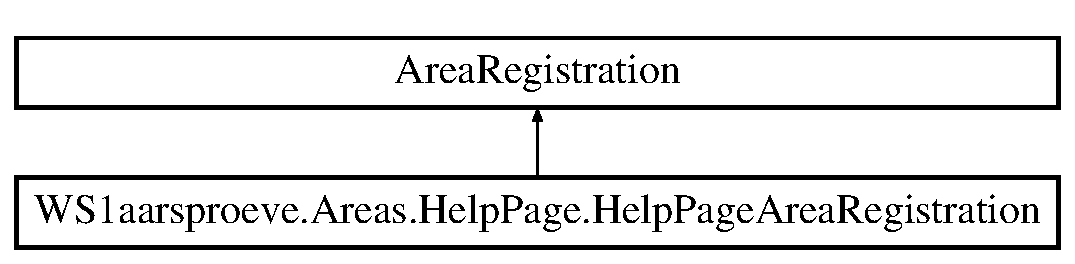
\includegraphics[height=2.000000cm]{class_w_s1aarsproeve_1_1_areas_1_1_help_page_1_1_help_page_area_registration}
\end{center}
\end{figure}
\subsection*{Public Member Functions}
\begin{DoxyCompactItemize}
\item 
\hypertarget{class_w_s1aarsproeve_1_1_areas_1_1_help_page_1_1_help_page_area_registration_a4521a2d5b11d5975c7a414674d44435e}{}override void {\bfseries Register\+Area} (Area\+Registration\+Context context)\label{class_w_s1aarsproeve_1_1_areas_1_1_help_page_1_1_help_page_area_registration_a4521a2d5b11d5975c7a414674d44435e}

\end{DoxyCompactItemize}
\subsection*{Properties}
\begin{DoxyCompactItemize}
\item 
\hypertarget{class_w_s1aarsproeve_1_1_areas_1_1_help_page_1_1_help_page_area_registration_af667b0bd093b2f9b247159990b0f7ea1}{}override string {\bfseries Area\+Name}\hspace{0.3cm}{\ttfamily  \mbox{[}get\mbox{]}}\label{class_w_s1aarsproeve_1_1_areas_1_1_help_page_1_1_help_page_area_registration_af667b0bd093b2f9b247159990b0f7ea1}

\end{DoxyCompactItemize}


The documentation for this class was generated from the following file\+:\begin{DoxyCompactItemize}
\item 
Documents/\+Git\+Hub/1-\/aarsproeve/1aarsproeve/\+W\+S1aarsproeve/\+Areas/\+Help\+Page/Help\+Page\+Area\+Registration.\+cs\end{DoxyCompactItemize}

\hypertarget{class__1aarsproeve_web_service_1_1_areas_1_1_help_page_1_1_help_page_area_registration}{}\section{\+\_\+1aarsproeve\+Web\+Service.\+Areas.\+Help\+Page.\+Help\+Page\+Area\+Registration Class Reference}
\label{class__1aarsproeve_web_service_1_1_areas_1_1_help_page_1_1_help_page_area_registration}\index{\+\_\+1aarsproeve\+Web\+Service.\+Areas.\+Help\+Page.\+Help\+Page\+Area\+Registration@{\+\_\+1aarsproeve\+Web\+Service.\+Areas.\+Help\+Page.\+Help\+Page\+Area\+Registration}}
Inheritance diagram for \+\_\+1aarsproeve\+Web\+Service.\+Areas.\+Help\+Page.\+Help\+Page\+Area\+Registration\+:\begin{figure}[H]
\begin{center}
\leavevmode
\includegraphics[height=2.000000cm]{class__1aarsproeve_web_service_1_1_areas_1_1_help_page_1_1_help_page_area_registration}
\end{center}
\end{figure}
\subsection*{Public Member Functions}
\begin{DoxyCompactItemize}
\item 
\hypertarget{class__1aarsproeve_web_service_1_1_areas_1_1_help_page_1_1_help_page_area_registration_a2d995fdeaeb65a3da6b712389c462b39}{}override void {\bfseries Register\+Area} (Area\+Registration\+Context context)\label{class__1aarsproeve_web_service_1_1_areas_1_1_help_page_1_1_help_page_area_registration_a2d995fdeaeb65a3da6b712389c462b39}

\end{DoxyCompactItemize}
\subsection*{Properties}
\begin{DoxyCompactItemize}
\item 
\hypertarget{class__1aarsproeve_web_service_1_1_areas_1_1_help_page_1_1_help_page_area_registration_a9402b3b3aba317e0afa36ff4ddf0593f}{}override string {\bfseries Area\+Name}\hspace{0.3cm}{\ttfamily  \mbox{[}get\mbox{]}}\label{class__1aarsproeve_web_service_1_1_areas_1_1_help_page_1_1_help_page_area_registration_a9402b3b3aba317e0afa36ff4ddf0593f}

\end{DoxyCompactItemize}


The documentation for this class was generated from the following file\+:\begin{DoxyCompactItemize}
\item 
C\+:/\+Users/\+Daniel\+Winther/\+Documents/\+Git\+Hub/1-\/aarsproeve/1aarsproeve/1aarsproeve\+Web\+Service/\+Areas/\+Help\+Page/Help\+Page\+Area\+Registration.\+cs\end{DoxyCompactItemize}

\hypertarget{class__1aarsproeve_web_service_1_1_areas_1_1_help_page_1_1_help_page_sample_generator}{}\section{\+\_\+1aarsproeve\+Web\+Service.\+Areas.\+Help\+Page.\+Help\+Page\+Sample\+Generator Class Reference}
\label{class__1aarsproeve_web_service_1_1_areas_1_1_help_page_1_1_help_page_sample_generator}\index{\+\_\+1aarsproeve\+Web\+Service.\+Areas.\+Help\+Page.\+Help\+Page\+Sample\+Generator@{\+\_\+1aarsproeve\+Web\+Service.\+Areas.\+Help\+Page.\+Help\+Page\+Sample\+Generator}}


This class will generate the samples for the help page.  


\subsection*{Public Member Functions}
\begin{DoxyCompactItemize}
\item 
\hyperlink{class__1aarsproeve_web_service_1_1_areas_1_1_help_page_1_1_help_page_sample_generator_aaffd24fef2501eaf464e7096fd4c02a7}{Help\+Page\+Sample\+Generator} ()
\begin{DoxyCompactList}\small\item\em Initializes a new instance of the \hyperlink{class__1aarsproeve_web_service_1_1_areas_1_1_help_page_1_1_help_page_sample_generator}{Help\+Page\+Sample\+Generator} class. \end{DoxyCompactList}\item 
I\+Dictionary$<$ Media\+Type\+Header\+Value, object $>$ \hyperlink{class__1aarsproeve_web_service_1_1_areas_1_1_help_page_1_1_help_page_sample_generator_a9cdb4f0b9852c9000a1519c984ac6f93}{Get\+Sample\+Requests} (Api\+Description api)
\begin{DoxyCompactList}\small\item\em Gets the request body samples for a given Api\+Description. \end{DoxyCompactList}\item 
I\+Dictionary$<$ Media\+Type\+Header\+Value, object $>$ \hyperlink{class__1aarsproeve_web_service_1_1_areas_1_1_help_page_1_1_help_page_sample_generator_a51d80ce95f3d1ed0aaa555a631dc8369}{Get\+Sample\+Responses} (Api\+Description api)
\begin{DoxyCompactList}\small\item\em Gets the response body samples for a given Api\+Description. \end{DoxyCompactList}\item 
virtual I\+Dictionary$<$ Media\+Type\+Header\+Value, object $>$ \hyperlink{class__1aarsproeve_web_service_1_1_areas_1_1_help_page_1_1_help_page_sample_generator_a4838c3b94a8ecabd38c519211ceeaa2b}{Get\+Sample} (Api\+Description api, \hyperlink{namespace__1aarsproeve_web_service_1_1_areas_1_1_help_page_a3b5e2312590d86c11aab0e939d9e102b}{Sample\+Direction} sample\+Direction)
\begin{DoxyCompactList}\small\item\em Gets the request or response body samples. \end{DoxyCompactList}\item 
virtual object \hyperlink{class__1aarsproeve_web_service_1_1_areas_1_1_help_page_1_1_help_page_sample_generator_a4b3866717927c231195a48f1826f99a6}{Get\+Action\+Sample} (string controller\+Name, string action\+Name, I\+Enumerable$<$ string $>$ parameter\+Names, Type type, Media\+Type\+Formatter formatter, Media\+Type\+Header\+Value media\+Type, \hyperlink{namespace__1aarsproeve_web_service_1_1_areas_1_1_help_page_a3b5e2312590d86c11aab0e939d9e102b}{Sample\+Direction} sample\+Direction)
\begin{DoxyCompactList}\small\item\em Search for samples that are provided directly through \hyperlink{class__1aarsproeve_web_service_1_1_areas_1_1_help_page_1_1_help_page_sample_generator_ad0321b323f21617bef877513f585c0a2}{Action\+Samples}. \end{DoxyCompactList}\item 
virtual object \hyperlink{class__1aarsproeve_web_service_1_1_areas_1_1_help_page_1_1_help_page_sample_generator_a5e04c38927cb05f3c416350bd3d8d7d8}{Get\+Sample\+Object} (Type type)
\begin{DoxyCompactList}\small\item\em Gets the sample object that will be serialized by the formatters. First, it will look at the \hyperlink{class__1aarsproeve_web_service_1_1_areas_1_1_help_page_1_1_help_page_sample_generator_aa9621fc1bc0621b656579d3967528dcc}{Sample\+Objects}. If no sample object is found, it will try to create one using Default\+Sample\+Object\+Factory (which wraps an \hyperlink{class__1aarsproeve_web_service_1_1_areas_1_1_help_page_1_1_object_generator}{Object\+Generator}) and other factories in \hyperlink{class__1aarsproeve_web_service_1_1_areas_1_1_help_page_1_1_help_page_sample_generator_a29295b515e45cebc44d8a111e9dd3d01}{Sample\+Object\+Factories}. \end{DoxyCompactList}\item 
virtual Type \hyperlink{class__1aarsproeve_web_service_1_1_areas_1_1_help_page_1_1_help_page_sample_generator_a5040f1ab4783209dd14860fe0b193496}{Resolve\+Http\+Request\+Message\+Type} (Api\+Description api)
\begin{DoxyCompactList}\small\item\em Resolves the actual type of System.\+Net.\+Http.\+Object\+Content$<$\+T$>$ passed to the System.\+Net.\+Http.\+Http\+Request\+Message in an action. \end{DoxyCompactList}\item 
virtual Type \hyperlink{class__1aarsproeve_web_service_1_1_areas_1_1_help_page_1_1_help_page_sample_generator_a4af0718be8a6369e37d905fb131e9448}{Resolve\+Type} (Api\+Description api, string controller\+Name, string action\+Name, I\+Enumerable$<$ string $>$ parameter\+Names, \hyperlink{namespace__1aarsproeve_web_service_1_1_areas_1_1_help_page_a3b5e2312590d86c11aab0e939d9e102b}{Sample\+Direction} sample\+Direction, out Collection$<$ Media\+Type\+Formatter $>$ formatters)
\begin{DoxyCompactList}\small\item\em Resolves the type of the action parameter or return value when Http\+Request\+Message or Http\+Response\+Message is used. \end{DoxyCompactList}\item 
virtual object \hyperlink{class__1aarsproeve_web_service_1_1_areas_1_1_help_page_1_1_help_page_sample_generator_ad78ea8663bf8d54d8a8ce4007ad58dba}{Write\+Sample\+Object\+Using\+Formatter} (Media\+Type\+Formatter formatter, object value, Type type, Media\+Type\+Header\+Value media\+Type)
\begin{DoxyCompactList}\small\item\em Writes the sample object using formatter. \end{DoxyCompactList}\end{DoxyCompactItemize}
\subsection*{Properties}
\begin{DoxyCompactItemize}
\item 
I\+Dictionary$<$ \hyperlink{class__1aarsproeve_web_service_1_1_areas_1_1_help_page_1_1_help_page_sample_key}{Help\+Page\+Sample\+Key}, Type $>$ \hyperlink{class__1aarsproeve_web_service_1_1_areas_1_1_help_page_1_1_help_page_sample_generator_a9f1ac86d102c5386627d7098a52d836f}{Actual\+Http\+Message\+Types}\hspace{0.3cm}{\ttfamily  \mbox{[}get, set\mbox{]}}
\begin{DoxyCompactList}\small\item\em Gets C\+L\+R types that are used as the content of Http\+Request\+Message or Http\+Response\+Message. \end{DoxyCompactList}\item 
I\+Dictionary$<$ \hyperlink{class__1aarsproeve_web_service_1_1_areas_1_1_help_page_1_1_help_page_sample_key}{Help\+Page\+Sample\+Key}, object $>$ \hyperlink{class__1aarsproeve_web_service_1_1_areas_1_1_help_page_1_1_help_page_sample_generator_ad0321b323f21617bef877513f585c0a2}{Action\+Samples}\hspace{0.3cm}{\ttfamily  \mbox{[}get, set\mbox{]}}
\begin{DoxyCompactList}\small\item\em Gets the objects that are used directly as samples for certain actions. \end{DoxyCompactList}\item 
I\+Dictionary$<$ Type, object $>$ \hyperlink{class__1aarsproeve_web_service_1_1_areas_1_1_help_page_1_1_help_page_sample_generator_aa9621fc1bc0621b656579d3967528dcc}{Sample\+Objects}\hspace{0.3cm}{\ttfamily  \mbox{[}get, set\mbox{]}}
\begin{DoxyCompactList}\small\item\em Gets the objects that are serialized as samples by the supported formatters. \end{DoxyCompactList}\item 
I\+List$<$ Func$<$ \hyperlink{class__1aarsproeve_web_service_1_1_areas_1_1_help_page_1_1_help_page_sample_generator}{Help\+Page\+Sample\+Generator}, Type, object $>$ $>$ \hyperlink{class__1aarsproeve_web_service_1_1_areas_1_1_help_page_1_1_help_page_sample_generator_a29295b515e45cebc44d8a111e9dd3d01}{Sample\+Object\+Factories}\hspace{0.3cm}{\ttfamily  \mbox{[}get\mbox{]}}
\begin{DoxyCompactList}\small\item\em Gets factories for the objects that the supported formatters will serialize as samples. Processed in order, stopping when the factory successfully returns a non-\/ object. \end{DoxyCompactList}\end{DoxyCompactItemize}


\subsection{Detailed Description}
This class will generate the samples for the help page. 



\subsection{Constructor \& Destructor Documentation}
\hypertarget{class__1aarsproeve_web_service_1_1_areas_1_1_help_page_1_1_help_page_sample_generator_aaffd24fef2501eaf464e7096fd4c02a7}{}\index{\+\_\+1aarsproeve\+Web\+Service\+::\+Areas\+::\+Help\+Page\+::\+Help\+Page\+Sample\+Generator@{\+\_\+1aarsproeve\+Web\+Service\+::\+Areas\+::\+Help\+Page\+::\+Help\+Page\+Sample\+Generator}!Help\+Page\+Sample\+Generator@{Help\+Page\+Sample\+Generator}}
\index{Help\+Page\+Sample\+Generator@{Help\+Page\+Sample\+Generator}!\+\_\+1aarsproeve\+Web\+Service\+::\+Areas\+::\+Help\+Page\+::\+Help\+Page\+Sample\+Generator@{\+\_\+1aarsproeve\+Web\+Service\+::\+Areas\+::\+Help\+Page\+::\+Help\+Page\+Sample\+Generator}}
\subsubsection[{Help\+Page\+Sample\+Generator}]{\setlength{\rightskip}{0pt plus 5cm}\+\_\+1aarsproeve\+Web\+Service.\+Areas.\+Help\+Page.\+Help\+Page\+Sample\+Generator.\+Help\+Page\+Sample\+Generator (
\begin{DoxyParamCaption}
{}
\end{DoxyParamCaption}
)}\label{class__1aarsproeve_web_service_1_1_areas_1_1_help_page_1_1_help_page_sample_generator_aaffd24fef2501eaf464e7096fd4c02a7}


Initializes a new instance of the \hyperlink{class__1aarsproeve_web_service_1_1_areas_1_1_help_page_1_1_help_page_sample_generator}{Help\+Page\+Sample\+Generator} class. 



\subsection{Member Function Documentation}
\hypertarget{class__1aarsproeve_web_service_1_1_areas_1_1_help_page_1_1_help_page_sample_generator_a4b3866717927c231195a48f1826f99a6}{}\index{\+\_\+1aarsproeve\+Web\+Service\+::\+Areas\+::\+Help\+Page\+::\+Help\+Page\+Sample\+Generator@{\+\_\+1aarsproeve\+Web\+Service\+::\+Areas\+::\+Help\+Page\+::\+Help\+Page\+Sample\+Generator}!Get\+Action\+Sample@{Get\+Action\+Sample}}
\index{Get\+Action\+Sample@{Get\+Action\+Sample}!\+\_\+1aarsproeve\+Web\+Service\+::\+Areas\+::\+Help\+Page\+::\+Help\+Page\+Sample\+Generator@{\+\_\+1aarsproeve\+Web\+Service\+::\+Areas\+::\+Help\+Page\+::\+Help\+Page\+Sample\+Generator}}
\subsubsection[{Get\+Action\+Sample}]{\setlength{\rightskip}{0pt plus 5cm}virtual object \+\_\+1aarsproeve\+Web\+Service.\+Areas.\+Help\+Page.\+Help\+Page\+Sample\+Generator.\+Get\+Action\+Sample (
\begin{DoxyParamCaption}
\item[{string}]{controller\+Name, }
\item[{string}]{action\+Name, }
\item[{I\+Enumerable$<$ string $>$}]{parameter\+Names, }
\item[{Type}]{type, }
\item[{Media\+Type\+Formatter}]{formatter, }
\item[{Media\+Type\+Header\+Value}]{media\+Type, }
\item[{{\bf Sample\+Direction}}]{sample\+Direction}
\end{DoxyParamCaption}
)\hspace{0.3cm}{\ttfamily [virtual]}}\label{class__1aarsproeve_web_service_1_1_areas_1_1_help_page_1_1_help_page_sample_generator_a4b3866717927c231195a48f1826f99a6}


Search for samples that are provided directly through \hyperlink{class__1aarsproeve_web_service_1_1_areas_1_1_help_page_1_1_help_page_sample_generator_ad0321b323f21617bef877513f585c0a2}{Action\+Samples}. 


\begin{DoxyParams}{Parameters}
{\em controller\+Name} & Name of the controller.\\
\hline
{\em action\+Name} & Name of the action.\\
\hline
{\em parameter\+Names} & The parameter names.\\
\hline
{\em type} & The C\+L\+R type.\\
\hline
{\em formatter} & The formatter.\\
\hline
{\em media\+Type} & The media type.\\
\hline
{\em sample\+Direction} & The value indicating whether the sample is for a request or for a response.\\
\hline
\end{DoxyParams}
\begin{DoxyReturn}{Returns}
The sample that matches the parameters.
\end{DoxyReturn}
\hypertarget{class__1aarsproeve_web_service_1_1_areas_1_1_help_page_1_1_help_page_sample_generator_a4838c3b94a8ecabd38c519211ceeaa2b}{}\index{\+\_\+1aarsproeve\+Web\+Service\+::\+Areas\+::\+Help\+Page\+::\+Help\+Page\+Sample\+Generator@{\+\_\+1aarsproeve\+Web\+Service\+::\+Areas\+::\+Help\+Page\+::\+Help\+Page\+Sample\+Generator}!Get\+Sample@{Get\+Sample}}
\index{Get\+Sample@{Get\+Sample}!\+\_\+1aarsproeve\+Web\+Service\+::\+Areas\+::\+Help\+Page\+::\+Help\+Page\+Sample\+Generator@{\+\_\+1aarsproeve\+Web\+Service\+::\+Areas\+::\+Help\+Page\+::\+Help\+Page\+Sample\+Generator}}
\subsubsection[{Get\+Sample}]{\setlength{\rightskip}{0pt plus 5cm}virtual I\+Dictionary$<$Media\+Type\+Header\+Value, object$>$ \+\_\+1aarsproeve\+Web\+Service.\+Areas.\+Help\+Page.\+Help\+Page\+Sample\+Generator.\+Get\+Sample (
\begin{DoxyParamCaption}
\item[{Api\+Description}]{api, }
\item[{{\bf Sample\+Direction}}]{sample\+Direction}
\end{DoxyParamCaption}
)\hspace{0.3cm}{\ttfamily [virtual]}}\label{class__1aarsproeve_web_service_1_1_areas_1_1_help_page_1_1_help_page_sample_generator_a4838c3b94a8ecabd38c519211ceeaa2b}


Gets the request or response body samples. 


\begin{DoxyParams}{Parameters}
{\em api} & The Api\+Description.\\
\hline
{\em sample\+Direction} & The value indicating whether the sample is for a request or for a response.\\
\hline
\end{DoxyParams}
\begin{DoxyReturn}{Returns}
The samples keyed by media type.
\end{DoxyReturn}
\hypertarget{class__1aarsproeve_web_service_1_1_areas_1_1_help_page_1_1_help_page_sample_generator_a5e04c38927cb05f3c416350bd3d8d7d8}{}\index{\+\_\+1aarsproeve\+Web\+Service\+::\+Areas\+::\+Help\+Page\+::\+Help\+Page\+Sample\+Generator@{\+\_\+1aarsproeve\+Web\+Service\+::\+Areas\+::\+Help\+Page\+::\+Help\+Page\+Sample\+Generator}!Get\+Sample\+Object@{Get\+Sample\+Object}}
\index{Get\+Sample\+Object@{Get\+Sample\+Object}!\+\_\+1aarsproeve\+Web\+Service\+::\+Areas\+::\+Help\+Page\+::\+Help\+Page\+Sample\+Generator@{\+\_\+1aarsproeve\+Web\+Service\+::\+Areas\+::\+Help\+Page\+::\+Help\+Page\+Sample\+Generator}}
\subsubsection[{Get\+Sample\+Object}]{\setlength{\rightskip}{0pt plus 5cm}virtual object \+\_\+1aarsproeve\+Web\+Service.\+Areas.\+Help\+Page.\+Help\+Page\+Sample\+Generator.\+Get\+Sample\+Object (
\begin{DoxyParamCaption}
\item[{Type}]{type}
\end{DoxyParamCaption}
)\hspace{0.3cm}{\ttfamily [virtual]}}\label{class__1aarsproeve_web_service_1_1_areas_1_1_help_page_1_1_help_page_sample_generator_a5e04c38927cb05f3c416350bd3d8d7d8}


Gets the sample object that will be serialized by the formatters. First, it will look at the \hyperlink{class__1aarsproeve_web_service_1_1_areas_1_1_help_page_1_1_help_page_sample_generator_aa9621fc1bc0621b656579d3967528dcc}{Sample\+Objects}. If no sample object is found, it will try to create one using Default\+Sample\+Object\+Factory (which wraps an \hyperlink{class__1aarsproeve_web_service_1_1_areas_1_1_help_page_1_1_object_generator}{Object\+Generator}) and other factories in \hyperlink{class__1aarsproeve_web_service_1_1_areas_1_1_help_page_1_1_help_page_sample_generator_a29295b515e45cebc44d8a111e9dd3d01}{Sample\+Object\+Factories}. 


\begin{DoxyParams}{Parameters}
{\em type} & The type.\\
\hline
\end{DoxyParams}
\begin{DoxyReturn}{Returns}
The sample object.
\end{DoxyReturn}
\hypertarget{class__1aarsproeve_web_service_1_1_areas_1_1_help_page_1_1_help_page_sample_generator_a9cdb4f0b9852c9000a1519c984ac6f93}{}\index{\+\_\+1aarsproeve\+Web\+Service\+::\+Areas\+::\+Help\+Page\+::\+Help\+Page\+Sample\+Generator@{\+\_\+1aarsproeve\+Web\+Service\+::\+Areas\+::\+Help\+Page\+::\+Help\+Page\+Sample\+Generator}!Get\+Sample\+Requests@{Get\+Sample\+Requests}}
\index{Get\+Sample\+Requests@{Get\+Sample\+Requests}!\+\_\+1aarsproeve\+Web\+Service\+::\+Areas\+::\+Help\+Page\+::\+Help\+Page\+Sample\+Generator@{\+\_\+1aarsproeve\+Web\+Service\+::\+Areas\+::\+Help\+Page\+::\+Help\+Page\+Sample\+Generator}}
\subsubsection[{Get\+Sample\+Requests}]{\setlength{\rightskip}{0pt plus 5cm}I\+Dictionary$<$Media\+Type\+Header\+Value, object$>$ \+\_\+1aarsproeve\+Web\+Service.\+Areas.\+Help\+Page.\+Help\+Page\+Sample\+Generator.\+Get\+Sample\+Requests (
\begin{DoxyParamCaption}
\item[{Api\+Description}]{api}
\end{DoxyParamCaption}
)}\label{class__1aarsproeve_web_service_1_1_areas_1_1_help_page_1_1_help_page_sample_generator_a9cdb4f0b9852c9000a1519c984ac6f93}


Gets the request body samples for a given Api\+Description. 


\begin{DoxyParams}{Parameters}
{\em api} & The Api\+Description.\\
\hline
\end{DoxyParams}
\begin{DoxyReturn}{Returns}
The samples keyed by media type.
\end{DoxyReturn}
\hypertarget{class__1aarsproeve_web_service_1_1_areas_1_1_help_page_1_1_help_page_sample_generator_a51d80ce95f3d1ed0aaa555a631dc8369}{}\index{\+\_\+1aarsproeve\+Web\+Service\+::\+Areas\+::\+Help\+Page\+::\+Help\+Page\+Sample\+Generator@{\+\_\+1aarsproeve\+Web\+Service\+::\+Areas\+::\+Help\+Page\+::\+Help\+Page\+Sample\+Generator}!Get\+Sample\+Responses@{Get\+Sample\+Responses}}
\index{Get\+Sample\+Responses@{Get\+Sample\+Responses}!\+\_\+1aarsproeve\+Web\+Service\+::\+Areas\+::\+Help\+Page\+::\+Help\+Page\+Sample\+Generator@{\+\_\+1aarsproeve\+Web\+Service\+::\+Areas\+::\+Help\+Page\+::\+Help\+Page\+Sample\+Generator}}
\subsubsection[{Get\+Sample\+Responses}]{\setlength{\rightskip}{0pt plus 5cm}I\+Dictionary$<$Media\+Type\+Header\+Value, object$>$ \+\_\+1aarsproeve\+Web\+Service.\+Areas.\+Help\+Page.\+Help\+Page\+Sample\+Generator.\+Get\+Sample\+Responses (
\begin{DoxyParamCaption}
\item[{Api\+Description}]{api}
\end{DoxyParamCaption}
)}\label{class__1aarsproeve_web_service_1_1_areas_1_1_help_page_1_1_help_page_sample_generator_a51d80ce95f3d1ed0aaa555a631dc8369}


Gets the response body samples for a given Api\+Description. 


\begin{DoxyParams}{Parameters}
{\em api} & The Api\+Description.\\
\hline
\end{DoxyParams}
\begin{DoxyReturn}{Returns}
The samples keyed by media type.
\end{DoxyReturn}
\hypertarget{class__1aarsproeve_web_service_1_1_areas_1_1_help_page_1_1_help_page_sample_generator_a5040f1ab4783209dd14860fe0b193496}{}\index{\+\_\+1aarsproeve\+Web\+Service\+::\+Areas\+::\+Help\+Page\+::\+Help\+Page\+Sample\+Generator@{\+\_\+1aarsproeve\+Web\+Service\+::\+Areas\+::\+Help\+Page\+::\+Help\+Page\+Sample\+Generator}!Resolve\+Http\+Request\+Message\+Type@{Resolve\+Http\+Request\+Message\+Type}}
\index{Resolve\+Http\+Request\+Message\+Type@{Resolve\+Http\+Request\+Message\+Type}!\+\_\+1aarsproeve\+Web\+Service\+::\+Areas\+::\+Help\+Page\+::\+Help\+Page\+Sample\+Generator@{\+\_\+1aarsproeve\+Web\+Service\+::\+Areas\+::\+Help\+Page\+::\+Help\+Page\+Sample\+Generator}}
\subsubsection[{Resolve\+Http\+Request\+Message\+Type}]{\setlength{\rightskip}{0pt plus 5cm}virtual Type \+\_\+1aarsproeve\+Web\+Service.\+Areas.\+Help\+Page.\+Help\+Page\+Sample\+Generator.\+Resolve\+Http\+Request\+Message\+Type (
\begin{DoxyParamCaption}
\item[{Api\+Description}]{api}
\end{DoxyParamCaption}
)\hspace{0.3cm}{\ttfamily [virtual]}}\label{class__1aarsproeve_web_service_1_1_areas_1_1_help_page_1_1_help_page_sample_generator_a5040f1ab4783209dd14860fe0b193496}


Resolves the actual type of System.\+Net.\+Http.\+Object\+Content$<$\+T$>$ passed to the System.\+Net.\+Http.\+Http\+Request\+Message in an action. 


\begin{DoxyParams}{Parameters}
{\em api} & The Api\+Description.\\
\hline
\end{DoxyParams}
\begin{DoxyReturn}{Returns}
The type.
\end{DoxyReturn}
\hypertarget{class__1aarsproeve_web_service_1_1_areas_1_1_help_page_1_1_help_page_sample_generator_a4af0718be8a6369e37d905fb131e9448}{}\index{\+\_\+1aarsproeve\+Web\+Service\+::\+Areas\+::\+Help\+Page\+::\+Help\+Page\+Sample\+Generator@{\+\_\+1aarsproeve\+Web\+Service\+::\+Areas\+::\+Help\+Page\+::\+Help\+Page\+Sample\+Generator}!Resolve\+Type@{Resolve\+Type}}
\index{Resolve\+Type@{Resolve\+Type}!\+\_\+1aarsproeve\+Web\+Service\+::\+Areas\+::\+Help\+Page\+::\+Help\+Page\+Sample\+Generator@{\+\_\+1aarsproeve\+Web\+Service\+::\+Areas\+::\+Help\+Page\+::\+Help\+Page\+Sample\+Generator}}
\subsubsection[{Resolve\+Type}]{\setlength{\rightskip}{0pt plus 5cm}virtual Type \+\_\+1aarsproeve\+Web\+Service.\+Areas.\+Help\+Page.\+Help\+Page\+Sample\+Generator.\+Resolve\+Type (
\begin{DoxyParamCaption}
\item[{Api\+Description}]{api, }
\item[{string}]{controller\+Name, }
\item[{string}]{action\+Name, }
\item[{I\+Enumerable$<$ string $>$}]{parameter\+Names, }
\item[{{\bf Sample\+Direction}}]{sample\+Direction, }
\item[{out Collection$<$ Media\+Type\+Formatter $>$}]{formatters}
\end{DoxyParamCaption}
)\hspace{0.3cm}{\ttfamily [virtual]}}\label{class__1aarsproeve_web_service_1_1_areas_1_1_help_page_1_1_help_page_sample_generator_a4af0718be8a6369e37d905fb131e9448}


Resolves the type of the action parameter or return value when Http\+Request\+Message or Http\+Response\+Message is used. 


\begin{DoxyParams}{Parameters}
{\em api} & The Api\+Description.\\
\hline
{\em controller\+Name} & Name of the controller.\\
\hline
{\em action\+Name} & Name of the action.\\
\hline
{\em parameter\+Names} & The parameter names.\\
\hline
{\em sample\+Direction} & The value indicating whether the sample is for a request or a response.\\
\hline
{\em formatters} & The formatters.\\
\hline
\end{DoxyParams}
\hypertarget{class__1aarsproeve_web_service_1_1_areas_1_1_help_page_1_1_help_page_sample_generator_ad78ea8663bf8d54d8a8ce4007ad58dba}{}\index{\+\_\+1aarsproeve\+Web\+Service\+::\+Areas\+::\+Help\+Page\+::\+Help\+Page\+Sample\+Generator@{\+\_\+1aarsproeve\+Web\+Service\+::\+Areas\+::\+Help\+Page\+::\+Help\+Page\+Sample\+Generator}!Write\+Sample\+Object\+Using\+Formatter@{Write\+Sample\+Object\+Using\+Formatter}}
\index{Write\+Sample\+Object\+Using\+Formatter@{Write\+Sample\+Object\+Using\+Formatter}!\+\_\+1aarsproeve\+Web\+Service\+::\+Areas\+::\+Help\+Page\+::\+Help\+Page\+Sample\+Generator@{\+\_\+1aarsproeve\+Web\+Service\+::\+Areas\+::\+Help\+Page\+::\+Help\+Page\+Sample\+Generator}}
\subsubsection[{Write\+Sample\+Object\+Using\+Formatter}]{\setlength{\rightskip}{0pt plus 5cm}virtual object \+\_\+1aarsproeve\+Web\+Service.\+Areas.\+Help\+Page.\+Help\+Page\+Sample\+Generator.\+Write\+Sample\+Object\+Using\+Formatter (
\begin{DoxyParamCaption}
\item[{Media\+Type\+Formatter}]{formatter, }
\item[{object}]{value, }
\item[{Type}]{type, }
\item[{Media\+Type\+Header\+Value}]{media\+Type}
\end{DoxyParamCaption}
)\hspace{0.3cm}{\ttfamily [virtual]}}\label{class__1aarsproeve_web_service_1_1_areas_1_1_help_page_1_1_help_page_sample_generator_ad78ea8663bf8d54d8a8ce4007ad58dba}


Writes the sample object using formatter. 


\begin{DoxyParams}{Parameters}
{\em formatter} & The formatter.\\
\hline
{\em value} & The value.\\
\hline
{\em type} & The type.\\
\hline
{\em media\+Type} & Type of the media.\\
\hline
\end{DoxyParams}
\begin{DoxyReturn}{Returns}

\end{DoxyReturn}


\subsection{Property Documentation}
\hypertarget{class__1aarsproeve_web_service_1_1_areas_1_1_help_page_1_1_help_page_sample_generator_ad0321b323f21617bef877513f585c0a2}{}\index{\+\_\+1aarsproeve\+Web\+Service\+::\+Areas\+::\+Help\+Page\+::\+Help\+Page\+Sample\+Generator@{\+\_\+1aarsproeve\+Web\+Service\+::\+Areas\+::\+Help\+Page\+::\+Help\+Page\+Sample\+Generator}!Action\+Samples@{Action\+Samples}}
\index{Action\+Samples@{Action\+Samples}!\+\_\+1aarsproeve\+Web\+Service\+::\+Areas\+::\+Help\+Page\+::\+Help\+Page\+Sample\+Generator@{\+\_\+1aarsproeve\+Web\+Service\+::\+Areas\+::\+Help\+Page\+::\+Help\+Page\+Sample\+Generator}}
\subsubsection[{Action\+Samples}]{\setlength{\rightskip}{0pt plus 5cm}I\+Dictionary$<${\bf Help\+Page\+Sample\+Key}, object$>$ \+\_\+1aarsproeve\+Web\+Service.\+Areas.\+Help\+Page.\+Help\+Page\+Sample\+Generator.\+Action\+Samples\hspace{0.3cm}{\ttfamily [get]}, {\ttfamily [set]}}\label{class__1aarsproeve_web_service_1_1_areas_1_1_help_page_1_1_help_page_sample_generator_ad0321b323f21617bef877513f585c0a2}


Gets the objects that are used directly as samples for certain actions. 

\hypertarget{class__1aarsproeve_web_service_1_1_areas_1_1_help_page_1_1_help_page_sample_generator_a9f1ac86d102c5386627d7098a52d836f}{}\index{\+\_\+1aarsproeve\+Web\+Service\+::\+Areas\+::\+Help\+Page\+::\+Help\+Page\+Sample\+Generator@{\+\_\+1aarsproeve\+Web\+Service\+::\+Areas\+::\+Help\+Page\+::\+Help\+Page\+Sample\+Generator}!Actual\+Http\+Message\+Types@{Actual\+Http\+Message\+Types}}
\index{Actual\+Http\+Message\+Types@{Actual\+Http\+Message\+Types}!\+\_\+1aarsproeve\+Web\+Service\+::\+Areas\+::\+Help\+Page\+::\+Help\+Page\+Sample\+Generator@{\+\_\+1aarsproeve\+Web\+Service\+::\+Areas\+::\+Help\+Page\+::\+Help\+Page\+Sample\+Generator}}
\subsubsection[{Actual\+Http\+Message\+Types}]{\setlength{\rightskip}{0pt plus 5cm}I\+Dictionary$<${\bf Help\+Page\+Sample\+Key}, Type$>$ \+\_\+1aarsproeve\+Web\+Service.\+Areas.\+Help\+Page.\+Help\+Page\+Sample\+Generator.\+Actual\+Http\+Message\+Types\hspace{0.3cm}{\ttfamily [get]}, {\ttfamily [set]}}\label{class__1aarsproeve_web_service_1_1_areas_1_1_help_page_1_1_help_page_sample_generator_a9f1ac86d102c5386627d7098a52d836f}


Gets C\+L\+R types that are used as the content of Http\+Request\+Message or Http\+Response\+Message. 

\hypertarget{class__1aarsproeve_web_service_1_1_areas_1_1_help_page_1_1_help_page_sample_generator_a29295b515e45cebc44d8a111e9dd3d01}{}\index{\+\_\+1aarsproeve\+Web\+Service\+::\+Areas\+::\+Help\+Page\+::\+Help\+Page\+Sample\+Generator@{\+\_\+1aarsproeve\+Web\+Service\+::\+Areas\+::\+Help\+Page\+::\+Help\+Page\+Sample\+Generator}!Sample\+Object\+Factories@{Sample\+Object\+Factories}}
\index{Sample\+Object\+Factories@{Sample\+Object\+Factories}!\+\_\+1aarsproeve\+Web\+Service\+::\+Areas\+::\+Help\+Page\+::\+Help\+Page\+Sample\+Generator@{\+\_\+1aarsproeve\+Web\+Service\+::\+Areas\+::\+Help\+Page\+::\+Help\+Page\+Sample\+Generator}}
\subsubsection[{Sample\+Object\+Factories}]{\setlength{\rightskip}{0pt plus 5cm}I\+List$<$Func$<${\bf Help\+Page\+Sample\+Generator}, Type, object$>$ $>$ \+\_\+1aarsproeve\+Web\+Service.\+Areas.\+Help\+Page.\+Help\+Page\+Sample\+Generator.\+Sample\+Object\+Factories\hspace{0.3cm}{\ttfamily [get]}}\label{class__1aarsproeve_web_service_1_1_areas_1_1_help_page_1_1_help_page_sample_generator_a29295b515e45cebc44d8a111e9dd3d01}


Gets factories for the objects that the supported formatters will serialize as samples. Processed in order, stopping when the factory successfully returns a non-\/ object. 

Collection includes just \hyperlink{class__1aarsproeve_web_service_1_1_areas_1_1_help_page_1_1_object_generator_ad47fd6b8894401475144cf522d8767d0}{Object\+Generator.\+Generate\+Object(\+Type)} initially. Use 
\begin{DoxyCode}
\hyperlink{class__1aarsproeve_web_service_1_1_areas_1_1_help_page_1_1_help_page_sample_generator_a29295b515e45cebc44d8a111e9dd3d01}{SampleObjectFactories}.Insert(0, func)
\end{DoxyCode}
 to provide an override and 
\begin{DoxyCode}
\hyperlink{class__1aarsproeve_web_service_1_1_areas_1_1_help_page_1_1_help_page_sample_generator_a29295b515e45cebc44d8a111e9dd3d01}{SampleObjectFactories}.Add(func)
\end{DoxyCode}
 to provide a fallback.\hypertarget{class__1aarsproeve_web_service_1_1_areas_1_1_help_page_1_1_help_page_sample_generator_aa9621fc1bc0621b656579d3967528dcc}{}\index{\+\_\+1aarsproeve\+Web\+Service\+::\+Areas\+::\+Help\+Page\+::\+Help\+Page\+Sample\+Generator@{\+\_\+1aarsproeve\+Web\+Service\+::\+Areas\+::\+Help\+Page\+::\+Help\+Page\+Sample\+Generator}!Sample\+Objects@{Sample\+Objects}}
\index{Sample\+Objects@{Sample\+Objects}!\+\_\+1aarsproeve\+Web\+Service\+::\+Areas\+::\+Help\+Page\+::\+Help\+Page\+Sample\+Generator@{\+\_\+1aarsproeve\+Web\+Service\+::\+Areas\+::\+Help\+Page\+::\+Help\+Page\+Sample\+Generator}}
\subsubsection[{Sample\+Objects}]{\setlength{\rightskip}{0pt plus 5cm}I\+Dictionary$<$Type, object$>$ \+\_\+1aarsproeve\+Web\+Service.\+Areas.\+Help\+Page.\+Help\+Page\+Sample\+Generator.\+Sample\+Objects\hspace{0.3cm}{\ttfamily [get]}, {\ttfamily [set]}}\label{class__1aarsproeve_web_service_1_1_areas_1_1_help_page_1_1_help_page_sample_generator_aa9621fc1bc0621b656579d3967528dcc}


Gets the objects that are serialized as samples by the supported formatters. 



The documentation for this class was generated from the following file\+:\begin{DoxyCompactItemize}
\item 
Documents/\+Git\+Hub/1-\/aarsproeve/1aarsproeve/1aarsproeve\+Web\+Service/\+Areas/\+Help\+Page/\+Sample\+Generation/Help\+Page\+Sample\+Generator.\+cs\end{DoxyCompactItemize}

\hypertarget{class_w_s1aarsproeve_1_1_areas_1_1_help_page_1_1_help_page_sample_generator}{}\section{W\+S1aarsproeve.\+Areas.\+Help\+Page.\+Help\+Page\+Sample\+Generator Class Reference}
\label{class_w_s1aarsproeve_1_1_areas_1_1_help_page_1_1_help_page_sample_generator}\index{W\+S1aarsproeve.\+Areas.\+Help\+Page.\+Help\+Page\+Sample\+Generator@{W\+S1aarsproeve.\+Areas.\+Help\+Page.\+Help\+Page\+Sample\+Generator}}


This class will generate the samples for the help page.  


\subsection*{Public Member Functions}
\begin{DoxyCompactItemize}
\item 
\hyperlink{class_w_s1aarsproeve_1_1_areas_1_1_help_page_1_1_help_page_sample_generator_ac280695fb6e9f681dd67a1e979216b4a}{Help\+Page\+Sample\+Generator} ()
\begin{DoxyCompactList}\small\item\em Initializes a new instance of the \hyperlink{class_w_s1aarsproeve_1_1_areas_1_1_help_page_1_1_help_page_sample_generator}{Help\+Page\+Sample\+Generator} class. \end{DoxyCompactList}\item 
I\+Dictionary$<$ Media\+Type\+Header\+Value, object $>$ \hyperlink{class_w_s1aarsproeve_1_1_areas_1_1_help_page_1_1_help_page_sample_generator_a77b8a544147892d516fd3d80e30fbd9b}{Get\+Sample\+Requests} (Api\+Description api)
\begin{DoxyCompactList}\small\item\em Gets the request body samples for a given Api\+Description. \end{DoxyCompactList}\item 
I\+Dictionary$<$ Media\+Type\+Header\+Value, object $>$ \hyperlink{class_w_s1aarsproeve_1_1_areas_1_1_help_page_1_1_help_page_sample_generator_a37feebe0544106124046a47e4a461744}{Get\+Sample\+Responses} (Api\+Description api)
\begin{DoxyCompactList}\small\item\em Gets the response body samples for a given Api\+Description. \end{DoxyCompactList}\item 
virtual I\+Dictionary$<$ Media\+Type\+Header\+Value, object $>$ \hyperlink{class_w_s1aarsproeve_1_1_areas_1_1_help_page_1_1_help_page_sample_generator_a14f7edab4919fa0a0038a8cbd1dbcb32}{Get\+Sample} (Api\+Description api, \hyperlink{namespace_w_s1aarsproeve_1_1_areas_1_1_help_page_a68a9a343f44949e9781196ca9699289c}{Sample\+Direction} sample\+Direction)
\begin{DoxyCompactList}\small\item\em Gets the request or response body samples. \end{DoxyCompactList}\item 
virtual object \hyperlink{class_w_s1aarsproeve_1_1_areas_1_1_help_page_1_1_help_page_sample_generator_ad3b94c7ea1f55a14da5c76821cd353f9}{Get\+Action\+Sample} (string controller\+Name, string action\+Name, I\+Enumerable$<$ string $>$ parameter\+Names, Type type, Media\+Type\+Formatter formatter, Media\+Type\+Header\+Value media\+Type, \hyperlink{namespace_w_s1aarsproeve_1_1_areas_1_1_help_page_a68a9a343f44949e9781196ca9699289c}{Sample\+Direction} sample\+Direction)
\begin{DoxyCompactList}\small\item\em Search for samples that are provided directly through \hyperlink{class_w_s1aarsproeve_1_1_areas_1_1_help_page_1_1_help_page_sample_generator_a2555dfa02ad5bcbfde218b929232c890}{Action\+Samples}. \end{DoxyCompactList}\item 
virtual object \hyperlink{class_w_s1aarsproeve_1_1_areas_1_1_help_page_1_1_help_page_sample_generator_aa6d7ce84b445586e5919d3c07a2ccc11}{Get\+Sample\+Object} (Type type)
\begin{DoxyCompactList}\small\item\em Gets the sample object that will be serialized by the formatters. First, it will look at the \hyperlink{class_w_s1aarsproeve_1_1_areas_1_1_help_page_1_1_help_page_sample_generator_a64ab17da769ced26a1908d1e48d5f9d0}{Sample\+Objects}. If no sample object is found, it will try to create one using Default\+Sample\+Object\+Factory (which wraps an \hyperlink{class_w_s1aarsproeve_1_1_areas_1_1_help_page_1_1_object_generator}{Object\+Generator}) and other factories in \hyperlink{class_w_s1aarsproeve_1_1_areas_1_1_help_page_1_1_help_page_sample_generator_aca3950f9dbe43316aa63aeaaeb1b05b1}{Sample\+Object\+Factories}. \end{DoxyCompactList}\item 
virtual Type \hyperlink{class_w_s1aarsproeve_1_1_areas_1_1_help_page_1_1_help_page_sample_generator_a3e37a9bba4063a2746c85965e29fd043}{Resolve\+Http\+Request\+Message\+Type} (Api\+Description api)
\begin{DoxyCompactList}\small\item\em Resolves the actual type of System.\+Net.\+Http.\+Object\+Content$<$\+T$>$ passed to the System.\+Net.\+Http.\+Http\+Request\+Message in an action. \end{DoxyCompactList}\item 
virtual Type \hyperlink{class_w_s1aarsproeve_1_1_areas_1_1_help_page_1_1_help_page_sample_generator_a9aeb8a00aaefa5872208f28a6c6f8cd2}{Resolve\+Type} (Api\+Description api, string controller\+Name, string action\+Name, I\+Enumerable$<$ string $>$ parameter\+Names, \hyperlink{namespace_w_s1aarsproeve_1_1_areas_1_1_help_page_a68a9a343f44949e9781196ca9699289c}{Sample\+Direction} sample\+Direction, out Collection$<$ Media\+Type\+Formatter $>$ formatters)
\begin{DoxyCompactList}\small\item\em Resolves the type of the action parameter or return value when Http\+Request\+Message or Http\+Response\+Message is used. \end{DoxyCompactList}\item 
virtual object \hyperlink{class_w_s1aarsproeve_1_1_areas_1_1_help_page_1_1_help_page_sample_generator_a40dd88815ced7cefa28aa3c247084c74}{Write\+Sample\+Object\+Using\+Formatter} (Media\+Type\+Formatter formatter, object value, Type type, Media\+Type\+Header\+Value media\+Type)
\begin{DoxyCompactList}\small\item\em Writes the sample object using formatter. \end{DoxyCompactList}\end{DoxyCompactItemize}
\subsection*{Properties}
\begin{DoxyCompactItemize}
\item 
I\+Dictionary$<$ \hyperlink{class_w_s1aarsproeve_1_1_areas_1_1_help_page_1_1_help_page_sample_key}{Help\+Page\+Sample\+Key}, Type $>$ \hyperlink{class_w_s1aarsproeve_1_1_areas_1_1_help_page_1_1_help_page_sample_generator_a9a18ba1bfe6a1ba41d8becee665a63b4}{Actual\+Http\+Message\+Types}\hspace{0.3cm}{\ttfamily  \mbox{[}get, set\mbox{]}}
\begin{DoxyCompactList}\small\item\em Gets C\+L\+R types that are used as the content of Http\+Request\+Message or Http\+Response\+Message. \end{DoxyCompactList}\item 
I\+Dictionary$<$ \hyperlink{class_w_s1aarsproeve_1_1_areas_1_1_help_page_1_1_help_page_sample_key}{Help\+Page\+Sample\+Key}, object $>$ \hyperlink{class_w_s1aarsproeve_1_1_areas_1_1_help_page_1_1_help_page_sample_generator_a2555dfa02ad5bcbfde218b929232c890}{Action\+Samples}\hspace{0.3cm}{\ttfamily  \mbox{[}get, set\mbox{]}}
\begin{DoxyCompactList}\small\item\em Gets the objects that are used directly as samples for certain actions. \end{DoxyCompactList}\item 
I\+Dictionary$<$ Type, object $>$ \hyperlink{class_w_s1aarsproeve_1_1_areas_1_1_help_page_1_1_help_page_sample_generator_a64ab17da769ced26a1908d1e48d5f9d0}{Sample\+Objects}\hspace{0.3cm}{\ttfamily  \mbox{[}get, set\mbox{]}}
\begin{DoxyCompactList}\small\item\em Gets the objects that are serialized as samples by the supported formatters. \end{DoxyCompactList}\item 
I\+List$<$ Func$<$ \hyperlink{class_w_s1aarsproeve_1_1_areas_1_1_help_page_1_1_help_page_sample_generator}{Help\+Page\+Sample\+Generator}, Type, object $>$ $>$ \hyperlink{class_w_s1aarsproeve_1_1_areas_1_1_help_page_1_1_help_page_sample_generator_aca3950f9dbe43316aa63aeaaeb1b05b1}{Sample\+Object\+Factories}\hspace{0.3cm}{\ttfamily  \mbox{[}get\mbox{]}}
\begin{DoxyCompactList}\small\item\em Gets factories for the objects that the supported formatters will serialize as samples. Processed in order, stopping when the factory successfully returns a non-\/ object. \end{DoxyCompactList}\end{DoxyCompactItemize}


\subsection{Detailed Description}
This class will generate the samples for the help page. 



\subsection{Constructor \& Destructor Documentation}
\hypertarget{class_w_s1aarsproeve_1_1_areas_1_1_help_page_1_1_help_page_sample_generator_ac280695fb6e9f681dd67a1e979216b4a}{}\index{W\+S1aarsproeve\+::\+Areas\+::\+Help\+Page\+::\+Help\+Page\+Sample\+Generator@{W\+S1aarsproeve\+::\+Areas\+::\+Help\+Page\+::\+Help\+Page\+Sample\+Generator}!Help\+Page\+Sample\+Generator@{Help\+Page\+Sample\+Generator}}
\index{Help\+Page\+Sample\+Generator@{Help\+Page\+Sample\+Generator}!W\+S1aarsproeve\+::\+Areas\+::\+Help\+Page\+::\+Help\+Page\+Sample\+Generator@{W\+S1aarsproeve\+::\+Areas\+::\+Help\+Page\+::\+Help\+Page\+Sample\+Generator}}
\subsubsection[{Help\+Page\+Sample\+Generator}]{\setlength{\rightskip}{0pt plus 5cm}W\+S1aarsproeve.\+Areas.\+Help\+Page.\+Help\+Page\+Sample\+Generator.\+Help\+Page\+Sample\+Generator (
\begin{DoxyParamCaption}
{}
\end{DoxyParamCaption}
)}\label{class_w_s1aarsproeve_1_1_areas_1_1_help_page_1_1_help_page_sample_generator_ac280695fb6e9f681dd67a1e979216b4a}


Initializes a new instance of the \hyperlink{class_w_s1aarsproeve_1_1_areas_1_1_help_page_1_1_help_page_sample_generator}{Help\+Page\+Sample\+Generator} class. 



\subsection{Member Function Documentation}
\hypertarget{class_w_s1aarsproeve_1_1_areas_1_1_help_page_1_1_help_page_sample_generator_ad3b94c7ea1f55a14da5c76821cd353f9}{}\index{W\+S1aarsproeve\+::\+Areas\+::\+Help\+Page\+::\+Help\+Page\+Sample\+Generator@{W\+S1aarsproeve\+::\+Areas\+::\+Help\+Page\+::\+Help\+Page\+Sample\+Generator}!Get\+Action\+Sample@{Get\+Action\+Sample}}
\index{Get\+Action\+Sample@{Get\+Action\+Sample}!W\+S1aarsproeve\+::\+Areas\+::\+Help\+Page\+::\+Help\+Page\+Sample\+Generator@{W\+S1aarsproeve\+::\+Areas\+::\+Help\+Page\+::\+Help\+Page\+Sample\+Generator}}
\subsubsection[{Get\+Action\+Sample}]{\setlength{\rightskip}{0pt plus 5cm}virtual object W\+S1aarsproeve.\+Areas.\+Help\+Page.\+Help\+Page\+Sample\+Generator.\+Get\+Action\+Sample (
\begin{DoxyParamCaption}
\item[{string}]{controller\+Name, }
\item[{string}]{action\+Name, }
\item[{I\+Enumerable$<$ string $>$}]{parameter\+Names, }
\item[{Type}]{type, }
\item[{Media\+Type\+Formatter}]{formatter, }
\item[{Media\+Type\+Header\+Value}]{media\+Type, }
\item[{{\bf Sample\+Direction}}]{sample\+Direction}
\end{DoxyParamCaption}
)\hspace{0.3cm}{\ttfamily [virtual]}}\label{class_w_s1aarsproeve_1_1_areas_1_1_help_page_1_1_help_page_sample_generator_ad3b94c7ea1f55a14da5c76821cd353f9}


Search for samples that are provided directly through \hyperlink{class_w_s1aarsproeve_1_1_areas_1_1_help_page_1_1_help_page_sample_generator_a2555dfa02ad5bcbfde218b929232c890}{Action\+Samples}. 


\begin{DoxyParams}{Parameters}
{\em controller\+Name} & Name of the controller.\\
\hline
{\em action\+Name} & Name of the action.\\
\hline
{\em parameter\+Names} & The parameter names.\\
\hline
{\em type} & The C\+L\+R type.\\
\hline
{\em formatter} & The formatter.\\
\hline
{\em media\+Type} & The media type.\\
\hline
{\em sample\+Direction} & The value indicating whether the sample is for a request or for a response.\\
\hline
\end{DoxyParams}
\begin{DoxyReturn}{Returns}
The sample that matches the parameters.
\end{DoxyReturn}
\hypertarget{class_w_s1aarsproeve_1_1_areas_1_1_help_page_1_1_help_page_sample_generator_a14f7edab4919fa0a0038a8cbd1dbcb32}{}\index{W\+S1aarsproeve\+::\+Areas\+::\+Help\+Page\+::\+Help\+Page\+Sample\+Generator@{W\+S1aarsproeve\+::\+Areas\+::\+Help\+Page\+::\+Help\+Page\+Sample\+Generator}!Get\+Sample@{Get\+Sample}}
\index{Get\+Sample@{Get\+Sample}!W\+S1aarsproeve\+::\+Areas\+::\+Help\+Page\+::\+Help\+Page\+Sample\+Generator@{W\+S1aarsproeve\+::\+Areas\+::\+Help\+Page\+::\+Help\+Page\+Sample\+Generator}}
\subsubsection[{Get\+Sample}]{\setlength{\rightskip}{0pt plus 5cm}virtual I\+Dictionary$<$Media\+Type\+Header\+Value, object$>$ W\+S1aarsproeve.\+Areas.\+Help\+Page.\+Help\+Page\+Sample\+Generator.\+Get\+Sample (
\begin{DoxyParamCaption}
\item[{Api\+Description}]{api, }
\item[{{\bf Sample\+Direction}}]{sample\+Direction}
\end{DoxyParamCaption}
)\hspace{0.3cm}{\ttfamily [virtual]}}\label{class_w_s1aarsproeve_1_1_areas_1_1_help_page_1_1_help_page_sample_generator_a14f7edab4919fa0a0038a8cbd1dbcb32}


Gets the request or response body samples. 


\begin{DoxyParams}{Parameters}
{\em api} & The Api\+Description.\\
\hline
{\em sample\+Direction} & The value indicating whether the sample is for a request or for a response.\\
\hline
\end{DoxyParams}
\begin{DoxyReturn}{Returns}
The samples keyed by media type.
\end{DoxyReturn}
\hypertarget{class_w_s1aarsproeve_1_1_areas_1_1_help_page_1_1_help_page_sample_generator_aa6d7ce84b445586e5919d3c07a2ccc11}{}\index{W\+S1aarsproeve\+::\+Areas\+::\+Help\+Page\+::\+Help\+Page\+Sample\+Generator@{W\+S1aarsproeve\+::\+Areas\+::\+Help\+Page\+::\+Help\+Page\+Sample\+Generator}!Get\+Sample\+Object@{Get\+Sample\+Object}}
\index{Get\+Sample\+Object@{Get\+Sample\+Object}!W\+S1aarsproeve\+::\+Areas\+::\+Help\+Page\+::\+Help\+Page\+Sample\+Generator@{W\+S1aarsproeve\+::\+Areas\+::\+Help\+Page\+::\+Help\+Page\+Sample\+Generator}}
\subsubsection[{Get\+Sample\+Object}]{\setlength{\rightskip}{0pt plus 5cm}virtual object W\+S1aarsproeve.\+Areas.\+Help\+Page.\+Help\+Page\+Sample\+Generator.\+Get\+Sample\+Object (
\begin{DoxyParamCaption}
\item[{Type}]{type}
\end{DoxyParamCaption}
)\hspace{0.3cm}{\ttfamily [virtual]}}\label{class_w_s1aarsproeve_1_1_areas_1_1_help_page_1_1_help_page_sample_generator_aa6d7ce84b445586e5919d3c07a2ccc11}


Gets the sample object that will be serialized by the formatters. First, it will look at the \hyperlink{class_w_s1aarsproeve_1_1_areas_1_1_help_page_1_1_help_page_sample_generator_a64ab17da769ced26a1908d1e48d5f9d0}{Sample\+Objects}. If no sample object is found, it will try to create one using Default\+Sample\+Object\+Factory (which wraps an \hyperlink{class_w_s1aarsproeve_1_1_areas_1_1_help_page_1_1_object_generator}{Object\+Generator}) and other factories in \hyperlink{class_w_s1aarsproeve_1_1_areas_1_1_help_page_1_1_help_page_sample_generator_aca3950f9dbe43316aa63aeaaeb1b05b1}{Sample\+Object\+Factories}. 


\begin{DoxyParams}{Parameters}
{\em type} & The type.\\
\hline
\end{DoxyParams}
\begin{DoxyReturn}{Returns}
The sample object.
\end{DoxyReturn}
\hypertarget{class_w_s1aarsproeve_1_1_areas_1_1_help_page_1_1_help_page_sample_generator_a77b8a544147892d516fd3d80e30fbd9b}{}\index{W\+S1aarsproeve\+::\+Areas\+::\+Help\+Page\+::\+Help\+Page\+Sample\+Generator@{W\+S1aarsproeve\+::\+Areas\+::\+Help\+Page\+::\+Help\+Page\+Sample\+Generator}!Get\+Sample\+Requests@{Get\+Sample\+Requests}}
\index{Get\+Sample\+Requests@{Get\+Sample\+Requests}!W\+S1aarsproeve\+::\+Areas\+::\+Help\+Page\+::\+Help\+Page\+Sample\+Generator@{W\+S1aarsproeve\+::\+Areas\+::\+Help\+Page\+::\+Help\+Page\+Sample\+Generator}}
\subsubsection[{Get\+Sample\+Requests}]{\setlength{\rightskip}{0pt plus 5cm}I\+Dictionary$<$Media\+Type\+Header\+Value, object$>$ W\+S1aarsproeve.\+Areas.\+Help\+Page.\+Help\+Page\+Sample\+Generator.\+Get\+Sample\+Requests (
\begin{DoxyParamCaption}
\item[{Api\+Description}]{api}
\end{DoxyParamCaption}
)}\label{class_w_s1aarsproeve_1_1_areas_1_1_help_page_1_1_help_page_sample_generator_a77b8a544147892d516fd3d80e30fbd9b}


Gets the request body samples for a given Api\+Description. 


\begin{DoxyParams}{Parameters}
{\em api} & The Api\+Description.\\
\hline
\end{DoxyParams}
\begin{DoxyReturn}{Returns}
The samples keyed by media type.
\end{DoxyReturn}
\hypertarget{class_w_s1aarsproeve_1_1_areas_1_1_help_page_1_1_help_page_sample_generator_a37feebe0544106124046a47e4a461744}{}\index{W\+S1aarsproeve\+::\+Areas\+::\+Help\+Page\+::\+Help\+Page\+Sample\+Generator@{W\+S1aarsproeve\+::\+Areas\+::\+Help\+Page\+::\+Help\+Page\+Sample\+Generator}!Get\+Sample\+Responses@{Get\+Sample\+Responses}}
\index{Get\+Sample\+Responses@{Get\+Sample\+Responses}!W\+S1aarsproeve\+::\+Areas\+::\+Help\+Page\+::\+Help\+Page\+Sample\+Generator@{W\+S1aarsproeve\+::\+Areas\+::\+Help\+Page\+::\+Help\+Page\+Sample\+Generator}}
\subsubsection[{Get\+Sample\+Responses}]{\setlength{\rightskip}{0pt plus 5cm}I\+Dictionary$<$Media\+Type\+Header\+Value, object$>$ W\+S1aarsproeve.\+Areas.\+Help\+Page.\+Help\+Page\+Sample\+Generator.\+Get\+Sample\+Responses (
\begin{DoxyParamCaption}
\item[{Api\+Description}]{api}
\end{DoxyParamCaption}
)}\label{class_w_s1aarsproeve_1_1_areas_1_1_help_page_1_1_help_page_sample_generator_a37feebe0544106124046a47e4a461744}


Gets the response body samples for a given Api\+Description. 


\begin{DoxyParams}{Parameters}
{\em api} & The Api\+Description.\\
\hline
\end{DoxyParams}
\begin{DoxyReturn}{Returns}
The samples keyed by media type.
\end{DoxyReturn}
\hypertarget{class_w_s1aarsproeve_1_1_areas_1_1_help_page_1_1_help_page_sample_generator_a3e37a9bba4063a2746c85965e29fd043}{}\index{W\+S1aarsproeve\+::\+Areas\+::\+Help\+Page\+::\+Help\+Page\+Sample\+Generator@{W\+S1aarsproeve\+::\+Areas\+::\+Help\+Page\+::\+Help\+Page\+Sample\+Generator}!Resolve\+Http\+Request\+Message\+Type@{Resolve\+Http\+Request\+Message\+Type}}
\index{Resolve\+Http\+Request\+Message\+Type@{Resolve\+Http\+Request\+Message\+Type}!W\+S1aarsproeve\+::\+Areas\+::\+Help\+Page\+::\+Help\+Page\+Sample\+Generator@{W\+S1aarsproeve\+::\+Areas\+::\+Help\+Page\+::\+Help\+Page\+Sample\+Generator}}
\subsubsection[{Resolve\+Http\+Request\+Message\+Type}]{\setlength{\rightskip}{0pt plus 5cm}virtual Type W\+S1aarsproeve.\+Areas.\+Help\+Page.\+Help\+Page\+Sample\+Generator.\+Resolve\+Http\+Request\+Message\+Type (
\begin{DoxyParamCaption}
\item[{Api\+Description}]{api}
\end{DoxyParamCaption}
)\hspace{0.3cm}{\ttfamily [virtual]}}\label{class_w_s1aarsproeve_1_1_areas_1_1_help_page_1_1_help_page_sample_generator_a3e37a9bba4063a2746c85965e29fd043}


Resolves the actual type of System.\+Net.\+Http.\+Object\+Content$<$\+T$>$ passed to the System.\+Net.\+Http.\+Http\+Request\+Message in an action. 


\begin{DoxyParams}{Parameters}
{\em api} & The Api\+Description.\\
\hline
\end{DoxyParams}
\begin{DoxyReturn}{Returns}
The type.
\end{DoxyReturn}
\hypertarget{class_w_s1aarsproeve_1_1_areas_1_1_help_page_1_1_help_page_sample_generator_a9aeb8a00aaefa5872208f28a6c6f8cd2}{}\index{W\+S1aarsproeve\+::\+Areas\+::\+Help\+Page\+::\+Help\+Page\+Sample\+Generator@{W\+S1aarsproeve\+::\+Areas\+::\+Help\+Page\+::\+Help\+Page\+Sample\+Generator}!Resolve\+Type@{Resolve\+Type}}
\index{Resolve\+Type@{Resolve\+Type}!W\+S1aarsproeve\+::\+Areas\+::\+Help\+Page\+::\+Help\+Page\+Sample\+Generator@{W\+S1aarsproeve\+::\+Areas\+::\+Help\+Page\+::\+Help\+Page\+Sample\+Generator}}
\subsubsection[{Resolve\+Type}]{\setlength{\rightskip}{0pt plus 5cm}virtual Type W\+S1aarsproeve.\+Areas.\+Help\+Page.\+Help\+Page\+Sample\+Generator.\+Resolve\+Type (
\begin{DoxyParamCaption}
\item[{Api\+Description}]{api, }
\item[{string}]{controller\+Name, }
\item[{string}]{action\+Name, }
\item[{I\+Enumerable$<$ string $>$}]{parameter\+Names, }
\item[{{\bf Sample\+Direction}}]{sample\+Direction, }
\item[{out Collection$<$ Media\+Type\+Formatter $>$}]{formatters}
\end{DoxyParamCaption}
)\hspace{0.3cm}{\ttfamily [virtual]}}\label{class_w_s1aarsproeve_1_1_areas_1_1_help_page_1_1_help_page_sample_generator_a9aeb8a00aaefa5872208f28a6c6f8cd2}


Resolves the type of the action parameter or return value when Http\+Request\+Message or Http\+Response\+Message is used. 


\begin{DoxyParams}{Parameters}
{\em api} & The Api\+Description.\\
\hline
{\em controller\+Name} & Name of the controller.\\
\hline
{\em action\+Name} & Name of the action.\\
\hline
{\em parameter\+Names} & The parameter names.\\
\hline
{\em sample\+Direction} & The value indicating whether the sample is for a request or a response.\\
\hline
{\em formatters} & The formatters.\\
\hline
\end{DoxyParams}
\hypertarget{class_w_s1aarsproeve_1_1_areas_1_1_help_page_1_1_help_page_sample_generator_a40dd88815ced7cefa28aa3c247084c74}{}\index{W\+S1aarsproeve\+::\+Areas\+::\+Help\+Page\+::\+Help\+Page\+Sample\+Generator@{W\+S1aarsproeve\+::\+Areas\+::\+Help\+Page\+::\+Help\+Page\+Sample\+Generator}!Write\+Sample\+Object\+Using\+Formatter@{Write\+Sample\+Object\+Using\+Formatter}}
\index{Write\+Sample\+Object\+Using\+Formatter@{Write\+Sample\+Object\+Using\+Formatter}!W\+S1aarsproeve\+::\+Areas\+::\+Help\+Page\+::\+Help\+Page\+Sample\+Generator@{W\+S1aarsproeve\+::\+Areas\+::\+Help\+Page\+::\+Help\+Page\+Sample\+Generator}}
\subsubsection[{Write\+Sample\+Object\+Using\+Formatter}]{\setlength{\rightskip}{0pt plus 5cm}virtual object W\+S1aarsproeve.\+Areas.\+Help\+Page.\+Help\+Page\+Sample\+Generator.\+Write\+Sample\+Object\+Using\+Formatter (
\begin{DoxyParamCaption}
\item[{Media\+Type\+Formatter}]{formatter, }
\item[{object}]{value, }
\item[{Type}]{type, }
\item[{Media\+Type\+Header\+Value}]{media\+Type}
\end{DoxyParamCaption}
)\hspace{0.3cm}{\ttfamily [virtual]}}\label{class_w_s1aarsproeve_1_1_areas_1_1_help_page_1_1_help_page_sample_generator_a40dd88815ced7cefa28aa3c247084c74}


Writes the sample object using formatter. 


\begin{DoxyParams}{Parameters}
{\em formatter} & The formatter.\\
\hline
{\em value} & The value.\\
\hline
{\em type} & The type.\\
\hline
{\em media\+Type} & Type of the media.\\
\hline
\end{DoxyParams}
\begin{DoxyReturn}{Returns}

\end{DoxyReturn}


\subsection{Property Documentation}
\hypertarget{class_w_s1aarsproeve_1_1_areas_1_1_help_page_1_1_help_page_sample_generator_a2555dfa02ad5bcbfde218b929232c890}{}\index{W\+S1aarsproeve\+::\+Areas\+::\+Help\+Page\+::\+Help\+Page\+Sample\+Generator@{W\+S1aarsproeve\+::\+Areas\+::\+Help\+Page\+::\+Help\+Page\+Sample\+Generator}!Action\+Samples@{Action\+Samples}}
\index{Action\+Samples@{Action\+Samples}!W\+S1aarsproeve\+::\+Areas\+::\+Help\+Page\+::\+Help\+Page\+Sample\+Generator@{W\+S1aarsproeve\+::\+Areas\+::\+Help\+Page\+::\+Help\+Page\+Sample\+Generator}}
\subsubsection[{Action\+Samples}]{\setlength{\rightskip}{0pt plus 5cm}I\+Dictionary$<${\bf Help\+Page\+Sample\+Key}, object$>$ W\+S1aarsproeve.\+Areas.\+Help\+Page.\+Help\+Page\+Sample\+Generator.\+Action\+Samples\hspace{0.3cm}{\ttfamily [get]}, {\ttfamily [set]}}\label{class_w_s1aarsproeve_1_1_areas_1_1_help_page_1_1_help_page_sample_generator_a2555dfa02ad5bcbfde218b929232c890}


Gets the objects that are used directly as samples for certain actions. 

\hypertarget{class_w_s1aarsproeve_1_1_areas_1_1_help_page_1_1_help_page_sample_generator_a9a18ba1bfe6a1ba41d8becee665a63b4}{}\index{W\+S1aarsproeve\+::\+Areas\+::\+Help\+Page\+::\+Help\+Page\+Sample\+Generator@{W\+S1aarsproeve\+::\+Areas\+::\+Help\+Page\+::\+Help\+Page\+Sample\+Generator}!Actual\+Http\+Message\+Types@{Actual\+Http\+Message\+Types}}
\index{Actual\+Http\+Message\+Types@{Actual\+Http\+Message\+Types}!W\+S1aarsproeve\+::\+Areas\+::\+Help\+Page\+::\+Help\+Page\+Sample\+Generator@{W\+S1aarsproeve\+::\+Areas\+::\+Help\+Page\+::\+Help\+Page\+Sample\+Generator}}
\subsubsection[{Actual\+Http\+Message\+Types}]{\setlength{\rightskip}{0pt plus 5cm}I\+Dictionary$<${\bf Help\+Page\+Sample\+Key}, Type$>$ W\+S1aarsproeve.\+Areas.\+Help\+Page.\+Help\+Page\+Sample\+Generator.\+Actual\+Http\+Message\+Types\hspace{0.3cm}{\ttfamily [get]}, {\ttfamily [set]}}\label{class_w_s1aarsproeve_1_1_areas_1_1_help_page_1_1_help_page_sample_generator_a9a18ba1bfe6a1ba41d8becee665a63b4}


Gets C\+L\+R types that are used as the content of Http\+Request\+Message or Http\+Response\+Message. 

\hypertarget{class_w_s1aarsproeve_1_1_areas_1_1_help_page_1_1_help_page_sample_generator_aca3950f9dbe43316aa63aeaaeb1b05b1}{}\index{W\+S1aarsproeve\+::\+Areas\+::\+Help\+Page\+::\+Help\+Page\+Sample\+Generator@{W\+S1aarsproeve\+::\+Areas\+::\+Help\+Page\+::\+Help\+Page\+Sample\+Generator}!Sample\+Object\+Factories@{Sample\+Object\+Factories}}
\index{Sample\+Object\+Factories@{Sample\+Object\+Factories}!W\+S1aarsproeve\+::\+Areas\+::\+Help\+Page\+::\+Help\+Page\+Sample\+Generator@{W\+S1aarsproeve\+::\+Areas\+::\+Help\+Page\+::\+Help\+Page\+Sample\+Generator}}
\subsubsection[{Sample\+Object\+Factories}]{\setlength{\rightskip}{0pt plus 5cm}I\+List$<$Func$<${\bf Help\+Page\+Sample\+Generator}, Type, object$>$ $>$ W\+S1aarsproeve.\+Areas.\+Help\+Page.\+Help\+Page\+Sample\+Generator.\+Sample\+Object\+Factories\hspace{0.3cm}{\ttfamily [get]}}\label{class_w_s1aarsproeve_1_1_areas_1_1_help_page_1_1_help_page_sample_generator_aca3950f9dbe43316aa63aeaaeb1b05b1}


Gets factories for the objects that the supported formatters will serialize as samples. Processed in order, stopping when the factory successfully returns a non-\/ object. 

Collection includes just \hyperlink{class_w_s1aarsproeve_1_1_areas_1_1_help_page_1_1_object_generator_ac9ee0b5d7e70f42b70a0785d17b661a7}{Object\+Generator.\+Generate\+Object(\+Type)} initially. Use 
\begin{DoxyCode}
\hyperlink{class_w_s1aarsproeve_1_1_areas_1_1_help_page_1_1_help_page_sample_generator_aca3950f9dbe43316aa63aeaaeb1b05b1}{SampleObjectFactories}.Insert(0, func)
\end{DoxyCode}
 to provide an override and 
\begin{DoxyCode}
\hyperlink{class_w_s1aarsproeve_1_1_areas_1_1_help_page_1_1_help_page_sample_generator_aca3950f9dbe43316aa63aeaaeb1b05b1}{SampleObjectFactories}.Add(func)
\end{DoxyCode}
 to provide a fallback.\hypertarget{class_w_s1aarsproeve_1_1_areas_1_1_help_page_1_1_help_page_sample_generator_a64ab17da769ced26a1908d1e48d5f9d0}{}\index{W\+S1aarsproeve\+::\+Areas\+::\+Help\+Page\+::\+Help\+Page\+Sample\+Generator@{W\+S1aarsproeve\+::\+Areas\+::\+Help\+Page\+::\+Help\+Page\+Sample\+Generator}!Sample\+Objects@{Sample\+Objects}}
\index{Sample\+Objects@{Sample\+Objects}!W\+S1aarsproeve\+::\+Areas\+::\+Help\+Page\+::\+Help\+Page\+Sample\+Generator@{W\+S1aarsproeve\+::\+Areas\+::\+Help\+Page\+::\+Help\+Page\+Sample\+Generator}}
\subsubsection[{Sample\+Objects}]{\setlength{\rightskip}{0pt plus 5cm}I\+Dictionary$<$Type, object$>$ W\+S1aarsproeve.\+Areas.\+Help\+Page.\+Help\+Page\+Sample\+Generator.\+Sample\+Objects\hspace{0.3cm}{\ttfamily [get]}, {\ttfamily [set]}}\label{class_w_s1aarsproeve_1_1_areas_1_1_help_page_1_1_help_page_sample_generator_a64ab17da769ced26a1908d1e48d5f9d0}


Gets the objects that are serialized as samples by the supported formatters. 



The documentation for this class was generated from the following file\+:\begin{DoxyCompactItemize}
\item 
Documents/\+Git\+Hub/1-\/aarsproeve/1aarsproeve/\+W\+S1aarsproeve/\+Areas/\+Help\+Page/\+Sample\+Generation/Help\+Page\+Sample\+Generator.\+cs\end{DoxyCompactItemize}

\hypertarget{class__1aarsproeve_web_service_1_1_areas_1_1_help_page_1_1_help_page_sample_key}{}\section{\+\_\+1aarsproeve\+Web\+Service.\+Areas.\+Help\+Page.\+Help\+Page\+Sample\+Key Class Reference}
\label{class__1aarsproeve_web_service_1_1_areas_1_1_help_page_1_1_help_page_sample_key}\index{\+\_\+1aarsproeve\+Web\+Service.\+Areas.\+Help\+Page.\+Help\+Page\+Sample\+Key@{\+\_\+1aarsproeve\+Web\+Service.\+Areas.\+Help\+Page.\+Help\+Page\+Sample\+Key}}


This is used to identify the place where the sample should be applied.  


\subsection*{Public Member Functions}
\begin{DoxyCompactItemize}
\item 
\hyperlink{class__1aarsproeve_web_service_1_1_areas_1_1_help_page_1_1_help_page_sample_key_ad5ad8423e1346cf212e19637088bc472}{Help\+Page\+Sample\+Key} (Media\+Type\+Header\+Value media\+Type)
\begin{DoxyCompactList}\small\item\em Creates a new \hyperlink{class__1aarsproeve_web_service_1_1_areas_1_1_help_page_1_1_help_page_sample_key}{Help\+Page\+Sample\+Key} based on media type. \end{DoxyCompactList}\item 
\hyperlink{class__1aarsproeve_web_service_1_1_areas_1_1_help_page_1_1_help_page_sample_key_a4170cca4dfffd21164c8ff7a54f20ac5}{Help\+Page\+Sample\+Key} (Media\+Type\+Header\+Value media\+Type, Type type)
\begin{DoxyCompactList}\small\item\em Creates a new \hyperlink{class__1aarsproeve_web_service_1_1_areas_1_1_help_page_1_1_help_page_sample_key}{Help\+Page\+Sample\+Key} based on media type and C\+L\+R type. \end{DoxyCompactList}\item 
\hyperlink{class__1aarsproeve_web_service_1_1_areas_1_1_help_page_1_1_help_page_sample_key_aeaaa386d273efbed71c42137489609b1}{Help\+Page\+Sample\+Key} (\hyperlink{namespace__1aarsproeve_web_service_1_1_areas_1_1_help_page_a3b5e2312590d86c11aab0e939d9e102b}{Sample\+Direction} sample\+Direction, string controller\+Name, string action\+Name, I\+Enumerable$<$ string $>$ parameter\+Names)
\begin{DoxyCompactList}\small\item\em Creates a new \hyperlink{class__1aarsproeve_web_service_1_1_areas_1_1_help_page_1_1_help_page_sample_key}{Help\+Page\+Sample\+Key} based on \hyperlink{class__1aarsproeve_web_service_1_1_areas_1_1_help_page_1_1_help_page_sample_key_a69980321c5a86fc11bbd2d4b3bca84ef}{Sample\+Direction}, controller name, action name and parameter names. \end{DoxyCompactList}\item 
\hyperlink{class__1aarsproeve_web_service_1_1_areas_1_1_help_page_1_1_help_page_sample_key_a37f83ad122302e2e6c2301bf0a7753ba}{Help\+Page\+Sample\+Key} (Media\+Type\+Header\+Value media\+Type, \hyperlink{namespace__1aarsproeve_web_service_1_1_areas_1_1_help_page_a3b5e2312590d86c11aab0e939d9e102b}{Sample\+Direction} sample\+Direction, string controller\+Name, string action\+Name, I\+Enumerable$<$ string $>$ parameter\+Names)
\begin{DoxyCompactList}\small\item\em Creates a new \hyperlink{class__1aarsproeve_web_service_1_1_areas_1_1_help_page_1_1_help_page_sample_key}{Help\+Page\+Sample\+Key} based on media type, \hyperlink{class__1aarsproeve_web_service_1_1_areas_1_1_help_page_1_1_help_page_sample_key_a69980321c5a86fc11bbd2d4b3bca84ef}{Sample\+Direction}, controller name, action name and parameter names. \end{DoxyCompactList}\item 
\hypertarget{class__1aarsproeve_web_service_1_1_areas_1_1_help_page_1_1_help_page_sample_key_aae1ef0cce0c728c5b4b766b6cfb1a19f}{}override bool {\bfseries Equals} (object obj)\label{class__1aarsproeve_web_service_1_1_areas_1_1_help_page_1_1_help_page_sample_key_aae1ef0cce0c728c5b4b766b6cfb1a19f}

\item 
\hypertarget{class__1aarsproeve_web_service_1_1_areas_1_1_help_page_1_1_help_page_sample_key_ab15eabbf1156828a8f95e890cd9b8cca}{}override int {\bfseries Get\+Hash\+Code} ()\label{class__1aarsproeve_web_service_1_1_areas_1_1_help_page_1_1_help_page_sample_key_ab15eabbf1156828a8f95e890cd9b8cca}

\end{DoxyCompactItemize}
\subsection*{Properties}
\begin{DoxyCompactItemize}
\item 
string \hyperlink{class__1aarsproeve_web_service_1_1_areas_1_1_help_page_1_1_help_page_sample_key_a83d3909e7f8daf7ab92060c21afef237}{Controller\+Name}\hspace{0.3cm}{\ttfamily  \mbox{[}get\mbox{]}}
\begin{DoxyCompactList}\small\item\em Gets the name of the controller. \end{DoxyCompactList}\item 
string \hyperlink{class__1aarsproeve_web_service_1_1_areas_1_1_help_page_1_1_help_page_sample_key_abb5930ab215393929bd5fc488c551f32}{Action\+Name}\hspace{0.3cm}{\ttfamily  \mbox{[}get\mbox{]}}
\begin{DoxyCompactList}\small\item\em Gets the name of the action. \end{DoxyCompactList}\item 
Media\+Type\+Header\+Value \hyperlink{class__1aarsproeve_web_service_1_1_areas_1_1_help_page_1_1_help_page_sample_key_a3db7a3c071a64389856208253ce6a8c3}{Media\+Type}\hspace{0.3cm}{\ttfamily  \mbox{[}get\mbox{]}}
\begin{DoxyCompactList}\small\item\em Gets the media type. \end{DoxyCompactList}\item 
Hash\+Set$<$ string $>$ \hyperlink{class__1aarsproeve_web_service_1_1_areas_1_1_help_page_1_1_help_page_sample_key_a2e76cfdbf00172ca1a0dedc0073aeb7b}{Parameter\+Names}\hspace{0.3cm}{\ttfamily  \mbox{[}get\mbox{]}}
\begin{DoxyCompactList}\small\item\em Gets the parameter names. \end{DoxyCompactList}\item 
\hypertarget{class__1aarsproeve_web_service_1_1_areas_1_1_help_page_1_1_help_page_sample_key_a06bee89f6540c17854e99d046dde0163}{}Type {\bfseries Parameter\+Type}\hspace{0.3cm}{\ttfamily  \mbox{[}get\mbox{]}}\label{class__1aarsproeve_web_service_1_1_areas_1_1_help_page_1_1_help_page_sample_key_a06bee89f6540c17854e99d046dde0163}

\item 
\hyperlink{namespace__1aarsproeve_web_service_1_1_areas_1_1_help_page_a3b5e2312590d86c11aab0e939d9e102b}{Sample\+Direction} \hyperlink{class__1aarsproeve_web_service_1_1_areas_1_1_help_page_1_1_help_page_sample_key_a69980321c5a86fc11bbd2d4b3bca84ef}{Sample\+Direction}\hspace{0.3cm}{\ttfamily  \mbox{[}get\mbox{]}}
\begin{DoxyCompactList}\small\item\em Gets the \hyperlink{class__1aarsproeve_web_service_1_1_areas_1_1_help_page_1_1_help_page_sample_key_a69980321c5a86fc11bbd2d4b3bca84ef}{Sample\+Direction}. \end{DoxyCompactList}\end{DoxyCompactItemize}


\subsection{Detailed Description}
This is used to identify the place where the sample should be applied. 



\subsection{Constructor \& Destructor Documentation}
\hypertarget{class__1aarsproeve_web_service_1_1_areas_1_1_help_page_1_1_help_page_sample_key_ad5ad8423e1346cf212e19637088bc472}{}\index{\+\_\+1aarsproeve\+Web\+Service\+::\+Areas\+::\+Help\+Page\+::\+Help\+Page\+Sample\+Key@{\+\_\+1aarsproeve\+Web\+Service\+::\+Areas\+::\+Help\+Page\+::\+Help\+Page\+Sample\+Key}!Help\+Page\+Sample\+Key@{Help\+Page\+Sample\+Key}}
\index{Help\+Page\+Sample\+Key@{Help\+Page\+Sample\+Key}!\+\_\+1aarsproeve\+Web\+Service\+::\+Areas\+::\+Help\+Page\+::\+Help\+Page\+Sample\+Key@{\+\_\+1aarsproeve\+Web\+Service\+::\+Areas\+::\+Help\+Page\+::\+Help\+Page\+Sample\+Key}}
\subsubsection[{Help\+Page\+Sample\+Key}]{\setlength{\rightskip}{0pt plus 5cm}\+\_\+1aarsproeve\+Web\+Service.\+Areas.\+Help\+Page.\+Help\+Page\+Sample\+Key.\+Help\+Page\+Sample\+Key (
\begin{DoxyParamCaption}
\item[{Media\+Type\+Header\+Value}]{media\+Type}
\end{DoxyParamCaption}
)\hspace{0.3cm}{\ttfamily [inline]}}\label{class__1aarsproeve_web_service_1_1_areas_1_1_help_page_1_1_help_page_sample_key_ad5ad8423e1346cf212e19637088bc472}


Creates a new \hyperlink{class__1aarsproeve_web_service_1_1_areas_1_1_help_page_1_1_help_page_sample_key}{Help\+Page\+Sample\+Key} based on media type. 


\begin{DoxyParams}{Parameters}
{\em media\+Type} & The media type.\\
\hline
\end{DoxyParams}
\hypertarget{class__1aarsproeve_web_service_1_1_areas_1_1_help_page_1_1_help_page_sample_key_a4170cca4dfffd21164c8ff7a54f20ac5}{}\index{\+\_\+1aarsproeve\+Web\+Service\+::\+Areas\+::\+Help\+Page\+::\+Help\+Page\+Sample\+Key@{\+\_\+1aarsproeve\+Web\+Service\+::\+Areas\+::\+Help\+Page\+::\+Help\+Page\+Sample\+Key}!Help\+Page\+Sample\+Key@{Help\+Page\+Sample\+Key}}
\index{Help\+Page\+Sample\+Key@{Help\+Page\+Sample\+Key}!\+\_\+1aarsproeve\+Web\+Service\+::\+Areas\+::\+Help\+Page\+::\+Help\+Page\+Sample\+Key@{\+\_\+1aarsproeve\+Web\+Service\+::\+Areas\+::\+Help\+Page\+::\+Help\+Page\+Sample\+Key}}
\subsubsection[{Help\+Page\+Sample\+Key}]{\setlength{\rightskip}{0pt plus 5cm}\+\_\+1aarsproeve\+Web\+Service.\+Areas.\+Help\+Page.\+Help\+Page\+Sample\+Key.\+Help\+Page\+Sample\+Key (
\begin{DoxyParamCaption}
\item[{Media\+Type\+Header\+Value}]{media\+Type, }
\item[{Type}]{type}
\end{DoxyParamCaption}
)\hspace{0.3cm}{\ttfamily [inline]}}\label{class__1aarsproeve_web_service_1_1_areas_1_1_help_page_1_1_help_page_sample_key_a4170cca4dfffd21164c8ff7a54f20ac5}


Creates a new \hyperlink{class__1aarsproeve_web_service_1_1_areas_1_1_help_page_1_1_help_page_sample_key}{Help\+Page\+Sample\+Key} based on media type and C\+L\+R type. 


\begin{DoxyParams}{Parameters}
{\em media\+Type} & The media type.\\
\hline
{\em type} & The C\+L\+R type.\\
\hline
\end{DoxyParams}
\hypertarget{class__1aarsproeve_web_service_1_1_areas_1_1_help_page_1_1_help_page_sample_key_aeaaa386d273efbed71c42137489609b1}{}\index{\+\_\+1aarsproeve\+Web\+Service\+::\+Areas\+::\+Help\+Page\+::\+Help\+Page\+Sample\+Key@{\+\_\+1aarsproeve\+Web\+Service\+::\+Areas\+::\+Help\+Page\+::\+Help\+Page\+Sample\+Key}!Help\+Page\+Sample\+Key@{Help\+Page\+Sample\+Key}}
\index{Help\+Page\+Sample\+Key@{Help\+Page\+Sample\+Key}!\+\_\+1aarsproeve\+Web\+Service\+::\+Areas\+::\+Help\+Page\+::\+Help\+Page\+Sample\+Key@{\+\_\+1aarsproeve\+Web\+Service\+::\+Areas\+::\+Help\+Page\+::\+Help\+Page\+Sample\+Key}}
\subsubsection[{Help\+Page\+Sample\+Key}]{\setlength{\rightskip}{0pt plus 5cm}\+\_\+1aarsproeve\+Web\+Service.\+Areas.\+Help\+Page.\+Help\+Page\+Sample\+Key.\+Help\+Page\+Sample\+Key (
\begin{DoxyParamCaption}
\item[{{\bf Sample\+Direction}}]{sample\+Direction, }
\item[{string}]{controller\+Name, }
\item[{string}]{action\+Name, }
\item[{I\+Enumerable$<$ string $>$}]{parameter\+Names}
\end{DoxyParamCaption}
)\hspace{0.3cm}{\ttfamily [inline]}}\label{class__1aarsproeve_web_service_1_1_areas_1_1_help_page_1_1_help_page_sample_key_aeaaa386d273efbed71c42137489609b1}


Creates a new \hyperlink{class__1aarsproeve_web_service_1_1_areas_1_1_help_page_1_1_help_page_sample_key}{Help\+Page\+Sample\+Key} based on \hyperlink{class__1aarsproeve_web_service_1_1_areas_1_1_help_page_1_1_help_page_sample_key_a69980321c5a86fc11bbd2d4b3bca84ef}{Sample\+Direction}, controller name, action name and parameter names. 


\begin{DoxyParams}{Parameters}
{\em sample\+Direction} & The \hyperlink{class__1aarsproeve_web_service_1_1_areas_1_1_help_page_1_1_help_page_sample_key_a69980321c5a86fc11bbd2d4b3bca84ef}{Sample\+Direction}.\\
\hline
{\em controller\+Name} & Name of the controller.\\
\hline
{\em action\+Name} & Name of the action.\\
\hline
{\em parameter\+Names} & The parameter names.\\
\hline
\end{DoxyParams}
\hypertarget{class__1aarsproeve_web_service_1_1_areas_1_1_help_page_1_1_help_page_sample_key_a37f83ad122302e2e6c2301bf0a7753ba}{}\index{\+\_\+1aarsproeve\+Web\+Service\+::\+Areas\+::\+Help\+Page\+::\+Help\+Page\+Sample\+Key@{\+\_\+1aarsproeve\+Web\+Service\+::\+Areas\+::\+Help\+Page\+::\+Help\+Page\+Sample\+Key}!Help\+Page\+Sample\+Key@{Help\+Page\+Sample\+Key}}
\index{Help\+Page\+Sample\+Key@{Help\+Page\+Sample\+Key}!\+\_\+1aarsproeve\+Web\+Service\+::\+Areas\+::\+Help\+Page\+::\+Help\+Page\+Sample\+Key@{\+\_\+1aarsproeve\+Web\+Service\+::\+Areas\+::\+Help\+Page\+::\+Help\+Page\+Sample\+Key}}
\subsubsection[{Help\+Page\+Sample\+Key}]{\setlength{\rightskip}{0pt plus 5cm}\+\_\+1aarsproeve\+Web\+Service.\+Areas.\+Help\+Page.\+Help\+Page\+Sample\+Key.\+Help\+Page\+Sample\+Key (
\begin{DoxyParamCaption}
\item[{Media\+Type\+Header\+Value}]{media\+Type, }
\item[{{\bf Sample\+Direction}}]{sample\+Direction, }
\item[{string}]{controller\+Name, }
\item[{string}]{action\+Name, }
\item[{I\+Enumerable$<$ string $>$}]{parameter\+Names}
\end{DoxyParamCaption}
)\hspace{0.3cm}{\ttfamily [inline]}}\label{class__1aarsproeve_web_service_1_1_areas_1_1_help_page_1_1_help_page_sample_key_a37f83ad122302e2e6c2301bf0a7753ba}


Creates a new \hyperlink{class__1aarsproeve_web_service_1_1_areas_1_1_help_page_1_1_help_page_sample_key}{Help\+Page\+Sample\+Key} based on media type, \hyperlink{class__1aarsproeve_web_service_1_1_areas_1_1_help_page_1_1_help_page_sample_key_a69980321c5a86fc11bbd2d4b3bca84ef}{Sample\+Direction}, controller name, action name and parameter names. 


\begin{DoxyParams}{Parameters}
{\em media\+Type} & The media type.\\
\hline
{\em sample\+Direction} & The \hyperlink{class__1aarsproeve_web_service_1_1_areas_1_1_help_page_1_1_help_page_sample_key_a69980321c5a86fc11bbd2d4b3bca84ef}{Sample\+Direction}.\\
\hline
{\em controller\+Name} & Name of the controller.\\
\hline
{\em action\+Name} & Name of the action.\\
\hline
{\em parameter\+Names} & The parameter names.\\
\hline
\end{DoxyParams}


\subsection{Property Documentation}
\hypertarget{class__1aarsproeve_web_service_1_1_areas_1_1_help_page_1_1_help_page_sample_key_abb5930ab215393929bd5fc488c551f32}{}\index{\+\_\+1aarsproeve\+Web\+Service\+::\+Areas\+::\+Help\+Page\+::\+Help\+Page\+Sample\+Key@{\+\_\+1aarsproeve\+Web\+Service\+::\+Areas\+::\+Help\+Page\+::\+Help\+Page\+Sample\+Key}!Action\+Name@{Action\+Name}}
\index{Action\+Name@{Action\+Name}!\+\_\+1aarsproeve\+Web\+Service\+::\+Areas\+::\+Help\+Page\+::\+Help\+Page\+Sample\+Key@{\+\_\+1aarsproeve\+Web\+Service\+::\+Areas\+::\+Help\+Page\+::\+Help\+Page\+Sample\+Key}}
\subsubsection[{Action\+Name}]{\setlength{\rightskip}{0pt plus 5cm}string \+\_\+1aarsproeve\+Web\+Service.\+Areas.\+Help\+Page.\+Help\+Page\+Sample\+Key.\+Action\+Name\hspace{0.3cm}{\ttfamily [get]}}\label{class__1aarsproeve_web_service_1_1_areas_1_1_help_page_1_1_help_page_sample_key_abb5930ab215393929bd5fc488c551f32}


Gets the name of the action. 

The name of the action. \hypertarget{class__1aarsproeve_web_service_1_1_areas_1_1_help_page_1_1_help_page_sample_key_a83d3909e7f8daf7ab92060c21afef237}{}\index{\+\_\+1aarsproeve\+Web\+Service\+::\+Areas\+::\+Help\+Page\+::\+Help\+Page\+Sample\+Key@{\+\_\+1aarsproeve\+Web\+Service\+::\+Areas\+::\+Help\+Page\+::\+Help\+Page\+Sample\+Key}!Controller\+Name@{Controller\+Name}}
\index{Controller\+Name@{Controller\+Name}!\+\_\+1aarsproeve\+Web\+Service\+::\+Areas\+::\+Help\+Page\+::\+Help\+Page\+Sample\+Key@{\+\_\+1aarsproeve\+Web\+Service\+::\+Areas\+::\+Help\+Page\+::\+Help\+Page\+Sample\+Key}}
\subsubsection[{Controller\+Name}]{\setlength{\rightskip}{0pt plus 5cm}string \+\_\+1aarsproeve\+Web\+Service.\+Areas.\+Help\+Page.\+Help\+Page\+Sample\+Key.\+Controller\+Name\hspace{0.3cm}{\ttfamily [get]}}\label{class__1aarsproeve_web_service_1_1_areas_1_1_help_page_1_1_help_page_sample_key_a83d3909e7f8daf7ab92060c21afef237}


Gets the name of the controller. 

The name of the controller. \hypertarget{class__1aarsproeve_web_service_1_1_areas_1_1_help_page_1_1_help_page_sample_key_a3db7a3c071a64389856208253ce6a8c3}{}\index{\+\_\+1aarsproeve\+Web\+Service\+::\+Areas\+::\+Help\+Page\+::\+Help\+Page\+Sample\+Key@{\+\_\+1aarsproeve\+Web\+Service\+::\+Areas\+::\+Help\+Page\+::\+Help\+Page\+Sample\+Key}!Media\+Type@{Media\+Type}}
\index{Media\+Type@{Media\+Type}!\+\_\+1aarsproeve\+Web\+Service\+::\+Areas\+::\+Help\+Page\+::\+Help\+Page\+Sample\+Key@{\+\_\+1aarsproeve\+Web\+Service\+::\+Areas\+::\+Help\+Page\+::\+Help\+Page\+Sample\+Key}}
\subsubsection[{Media\+Type}]{\setlength{\rightskip}{0pt plus 5cm}Media\+Type\+Header\+Value \+\_\+1aarsproeve\+Web\+Service.\+Areas.\+Help\+Page.\+Help\+Page\+Sample\+Key.\+Media\+Type\hspace{0.3cm}{\ttfamily [get]}}\label{class__1aarsproeve_web_service_1_1_areas_1_1_help_page_1_1_help_page_sample_key_a3db7a3c071a64389856208253ce6a8c3}


Gets the media type. 

The media type. \hypertarget{class__1aarsproeve_web_service_1_1_areas_1_1_help_page_1_1_help_page_sample_key_a2e76cfdbf00172ca1a0dedc0073aeb7b}{}\index{\+\_\+1aarsproeve\+Web\+Service\+::\+Areas\+::\+Help\+Page\+::\+Help\+Page\+Sample\+Key@{\+\_\+1aarsproeve\+Web\+Service\+::\+Areas\+::\+Help\+Page\+::\+Help\+Page\+Sample\+Key}!Parameter\+Names@{Parameter\+Names}}
\index{Parameter\+Names@{Parameter\+Names}!\+\_\+1aarsproeve\+Web\+Service\+::\+Areas\+::\+Help\+Page\+::\+Help\+Page\+Sample\+Key@{\+\_\+1aarsproeve\+Web\+Service\+::\+Areas\+::\+Help\+Page\+::\+Help\+Page\+Sample\+Key}}
\subsubsection[{Parameter\+Names}]{\setlength{\rightskip}{0pt plus 5cm}Hash\+Set$<$string$>$ \+\_\+1aarsproeve\+Web\+Service.\+Areas.\+Help\+Page.\+Help\+Page\+Sample\+Key.\+Parameter\+Names\hspace{0.3cm}{\ttfamily [get]}}\label{class__1aarsproeve_web_service_1_1_areas_1_1_help_page_1_1_help_page_sample_key_a2e76cfdbf00172ca1a0dedc0073aeb7b}


Gets the parameter names. 

\hypertarget{class__1aarsproeve_web_service_1_1_areas_1_1_help_page_1_1_help_page_sample_key_a69980321c5a86fc11bbd2d4b3bca84ef}{}\index{\+\_\+1aarsproeve\+Web\+Service\+::\+Areas\+::\+Help\+Page\+::\+Help\+Page\+Sample\+Key@{\+\_\+1aarsproeve\+Web\+Service\+::\+Areas\+::\+Help\+Page\+::\+Help\+Page\+Sample\+Key}!Sample\+Direction@{Sample\+Direction}}
\index{Sample\+Direction@{Sample\+Direction}!\+\_\+1aarsproeve\+Web\+Service\+::\+Areas\+::\+Help\+Page\+::\+Help\+Page\+Sample\+Key@{\+\_\+1aarsproeve\+Web\+Service\+::\+Areas\+::\+Help\+Page\+::\+Help\+Page\+Sample\+Key}}
\subsubsection[{Sample\+Direction}]{\setlength{\rightskip}{0pt plus 5cm}{\bf Sample\+Direction} \+\_\+1aarsproeve\+Web\+Service.\+Areas.\+Help\+Page.\+Help\+Page\+Sample\+Key.\+Sample\+Direction\hspace{0.3cm}{\ttfamily [get]}}\label{class__1aarsproeve_web_service_1_1_areas_1_1_help_page_1_1_help_page_sample_key_a69980321c5a86fc11bbd2d4b3bca84ef}


Gets the \hyperlink{class__1aarsproeve_web_service_1_1_areas_1_1_help_page_1_1_help_page_sample_key_a69980321c5a86fc11bbd2d4b3bca84ef}{Sample\+Direction}. 



The documentation for this class was generated from the following file\+:\begin{DoxyCompactItemize}
\item 
Documents/\+Git\+Hub/1-\/aarsproeve/1aarsproeve/1aarsproeve\+Web\+Service/\+Areas/\+Help\+Page/\+Sample\+Generation/Help\+Page\+Sample\+Key.\+cs\end{DoxyCompactItemize}

\hypertarget{class_w_s1aarsproeve_1_1_areas_1_1_help_page_1_1_help_page_sample_key}{}\section{W\+S1aarsproeve.\+Areas.\+Help\+Page.\+Help\+Page\+Sample\+Key Class Reference}
\label{class_w_s1aarsproeve_1_1_areas_1_1_help_page_1_1_help_page_sample_key}\index{W\+S1aarsproeve.\+Areas.\+Help\+Page.\+Help\+Page\+Sample\+Key@{W\+S1aarsproeve.\+Areas.\+Help\+Page.\+Help\+Page\+Sample\+Key}}


This is used to identify the place where the sample should be applied.  


\subsection*{Public Member Functions}
\begin{DoxyCompactItemize}
\item 
\hyperlink{class_w_s1aarsproeve_1_1_areas_1_1_help_page_1_1_help_page_sample_key_ab9bf1ca3723aca11ab9a912101238018}{Help\+Page\+Sample\+Key} (Media\+Type\+Header\+Value media\+Type)
\begin{DoxyCompactList}\small\item\em Creates a new \hyperlink{class_w_s1aarsproeve_1_1_areas_1_1_help_page_1_1_help_page_sample_key}{Help\+Page\+Sample\+Key} based on media type. \end{DoxyCompactList}\item 
\hyperlink{class_w_s1aarsproeve_1_1_areas_1_1_help_page_1_1_help_page_sample_key_a40981c473e9ae2211e0e7bcfaceda021}{Help\+Page\+Sample\+Key} (Media\+Type\+Header\+Value media\+Type, Type type)
\begin{DoxyCompactList}\small\item\em Creates a new \hyperlink{class_w_s1aarsproeve_1_1_areas_1_1_help_page_1_1_help_page_sample_key}{Help\+Page\+Sample\+Key} based on media type and C\+L\+R type. \end{DoxyCompactList}\item 
\hyperlink{class_w_s1aarsproeve_1_1_areas_1_1_help_page_1_1_help_page_sample_key_a71025181698b607423d176758aacfe98}{Help\+Page\+Sample\+Key} (\hyperlink{namespace_w_s1aarsproeve_1_1_areas_1_1_help_page_a68a9a343f44949e9781196ca9699289c}{Sample\+Direction} sample\+Direction, string controller\+Name, string action\+Name, I\+Enumerable$<$ string $>$ parameter\+Names)
\begin{DoxyCompactList}\small\item\em Creates a new \hyperlink{class_w_s1aarsproeve_1_1_areas_1_1_help_page_1_1_help_page_sample_key}{Help\+Page\+Sample\+Key} based on \hyperlink{class_w_s1aarsproeve_1_1_areas_1_1_help_page_1_1_help_page_sample_key_a4d02725ac4f265d06bfb42d669de3edc}{Sample\+Direction}, controller name, action name and parameter names. \end{DoxyCompactList}\item 
\hyperlink{class_w_s1aarsproeve_1_1_areas_1_1_help_page_1_1_help_page_sample_key_a67b5bb876d265c39a0fb58529fbe28c5}{Help\+Page\+Sample\+Key} (Media\+Type\+Header\+Value media\+Type, \hyperlink{namespace_w_s1aarsproeve_1_1_areas_1_1_help_page_a68a9a343f44949e9781196ca9699289c}{Sample\+Direction} sample\+Direction, string controller\+Name, string action\+Name, I\+Enumerable$<$ string $>$ parameter\+Names)
\begin{DoxyCompactList}\small\item\em Creates a new \hyperlink{class_w_s1aarsproeve_1_1_areas_1_1_help_page_1_1_help_page_sample_key}{Help\+Page\+Sample\+Key} based on media type, \hyperlink{class_w_s1aarsproeve_1_1_areas_1_1_help_page_1_1_help_page_sample_key_a4d02725ac4f265d06bfb42d669de3edc}{Sample\+Direction}, controller name, action name and parameter names. \end{DoxyCompactList}\item 
\hypertarget{class_w_s1aarsproeve_1_1_areas_1_1_help_page_1_1_help_page_sample_key_a5764053ee93d0f69aa7eb5025a069eab}{}override bool {\bfseries Equals} (object obj)\label{class_w_s1aarsproeve_1_1_areas_1_1_help_page_1_1_help_page_sample_key_a5764053ee93d0f69aa7eb5025a069eab}

\item 
\hypertarget{class_w_s1aarsproeve_1_1_areas_1_1_help_page_1_1_help_page_sample_key_ae9534362f22204b8ebbaaca5971e7604}{}override int {\bfseries Get\+Hash\+Code} ()\label{class_w_s1aarsproeve_1_1_areas_1_1_help_page_1_1_help_page_sample_key_ae9534362f22204b8ebbaaca5971e7604}

\end{DoxyCompactItemize}
\subsection*{Properties}
\begin{DoxyCompactItemize}
\item 
string \hyperlink{class_w_s1aarsproeve_1_1_areas_1_1_help_page_1_1_help_page_sample_key_a6d46b214a46fe71b0d7529c37191aa4f}{Controller\+Name}\hspace{0.3cm}{\ttfamily  \mbox{[}get\mbox{]}}
\begin{DoxyCompactList}\small\item\em Gets the name of the controller. \end{DoxyCompactList}\item 
string \hyperlink{class_w_s1aarsproeve_1_1_areas_1_1_help_page_1_1_help_page_sample_key_a04142e3fa553ca3923d5bc56946fc191}{Action\+Name}\hspace{0.3cm}{\ttfamily  \mbox{[}get\mbox{]}}
\begin{DoxyCompactList}\small\item\em Gets the name of the action. \end{DoxyCompactList}\item 
Media\+Type\+Header\+Value \hyperlink{class_w_s1aarsproeve_1_1_areas_1_1_help_page_1_1_help_page_sample_key_a0f7ca7edc665a4ec1659e060fe66bdff}{Media\+Type}\hspace{0.3cm}{\ttfamily  \mbox{[}get\mbox{]}}
\begin{DoxyCompactList}\small\item\em Gets the media type. \end{DoxyCompactList}\item 
Hash\+Set$<$ string $>$ \hyperlink{class_w_s1aarsproeve_1_1_areas_1_1_help_page_1_1_help_page_sample_key_a49d37bbf913e01d893ea7a6e2975dcee}{Parameter\+Names}\hspace{0.3cm}{\ttfamily  \mbox{[}get\mbox{]}}
\begin{DoxyCompactList}\small\item\em Gets the parameter names. \end{DoxyCompactList}\item 
\hypertarget{class_w_s1aarsproeve_1_1_areas_1_1_help_page_1_1_help_page_sample_key_ad77ec60047fa2968b7ce0e167db11b89}{}Type {\bfseries Parameter\+Type}\hspace{0.3cm}{\ttfamily  \mbox{[}get\mbox{]}}\label{class_w_s1aarsproeve_1_1_areas_1_1_help_page_1_1_help_page_sample_key_ad77ec60047fa2968b7ce0e167db11b89}

\item 
\hyperlink{namespace_w_s1aarsproeve_1_1_areas_1_1_help_page_a68a9a343f44949e9781196ca9699289c}{Sample\+Direction} \hyperlink{class_w_s1aarsproeve_1_1_areas_1_1_help_page_1_1_help_page_sample_key_a4d02725ac4f265d06bfb42d669de3edc}{Sample\+Direction}\hspace{0.3cm}{\ttfamily  \mbox{[}get\mbox{]}}
\begin{DoxyCompactList}\small\item\em Gets the \hyperlink{class_w_s1aarsproeve_1_1_areas_1_1_help_page_1_1_help_page_sample_key_a4d02725ac4f265d06bfb42d669de3edc}{Sample\+Direction}. \end{DoxyCompactList}\end{DoxyCompactItemize}


\subsection{Detailed Description}
This is used to identify the place where the sample should be applied. 



\subsection{Constructor \& Destructor Documentation}
\hypertarget{class_w_s1aarsproeve_1_1_areas_1_1_help_page_1_1_help_page_sample_key_ab9bf1ca3723aca11ab9a912101238018}{}\index{W\+S1aarsproeve\+::\+Areas\+::\+Help\+Page\+::\+Help\+Page\+Sample\+Key@{W\+S1aarsproeve\+::\+Areas\+::\+Help\+Page\+::\+Help\+Page\+Sample\+Key}!Help\+Page\+Sample\+Key@{Help\+Page\+Sample\+Key}}
\index{Help\+Page\+Sample\+Key@{Help\+Page\+Sample\+Key}!W\+S1aarsproeve\+::\+Areas\+::\+Help\+Page\+::\+Help\+Page\+Sample\+Key@{W\+S1aarsproeve\+::\+Areas\+::\+Help\+Page\+::\+Help\+Page\+Sample\+Key}}
\subsubsection[{Help\+Page\+Sample\+Key}]{\setlength{\rightskip}{0pt plus 5cm}W\+S1aarsproeve.\+Areas.\+Help\+Page.\+Help\+Page\+Sample\+Key.\+Help\+Page\+Sample\+Key (
\begin{DoxyParamCaption}
\item[{Media\+Type\+Header\+Value}]{media\+Type}
\end{DoxyParamCaption}
)}\label{class_w_s1aarsproeve_1_1_areas_1_1_help_page_1_1_help_page_sample_key_ab9bf1ca3723aca11ab9a912101238018}


Creates a new \hyperlink{class_w_s1aarsproeve_1_1_areas_1_1_help_page_1_1_help_page_sample_key}{Help\+Page\+Sample\+Key} based on media type. 


\begin{DoxyParams}{Parameters}
{\em media\+Type} & The media type.\\
\hline
\end{DoxyParams}
\hypertarget{class_w_s1aarsproeve_1_1_areas_1_1_help_page_1_1_help_page_sample_key_a40981c473e9ae2211e0e7bcfaceda021}{}\index{W\+S1aarsproeve\+::\+Areas\+::\+Help\+Page\+::\+Help\+Page\+Sample\+Key@{W\+S1aarsproeve\+::\+Areas\+::\+Help\+Page\+::\+Help\+Page\+Sample\+Key}!Help\+Page\+Sample\+Key@{Help\+Page\+Sample\+Key}}
\index{Help\+Page\+Sample\+Key@{Help\+Page\+Sample\+Key}!W\+S1aarsproeve\+::\+Areas\+::\+Help\+Page\+::\+Help\+Page\+Sample\+Key@{W\+S1aarsproeve\+::\+Areas\+::\+Help\+Page\+::\+Help\+Page\+Sample\+Key}}
\subsubsection[{Help\+Page\+Sample\+Key}]{\setlength{\rightskip}{0pt plus 5cm}W\+S1aarsproeve.\+Areas.\+Help\+Page.\+Help\+Page\+Sample\+Key.\+Help\+Page\+Sample\+Key (
\begin{DoxyParamCaption}
\item[{Media\+Type\+Header\+Value}]{media\+Type, }
\item[{Type}]{type}
\end{DoxyParamCaption}
)}\label{class_w_s1aarsproeve_1_1_areas_1_1_help_page_1_1_help_page_sample_key_a40981c473e9ae2211e0e7bcfaceda021}


Creates a new \hyperlink{class_w_s1aarsproeve_1_1_areas_1_1_help_page_1_1_help_page_sample_key}{Help\+Page\+Sample\+Key} based on media type and C\+L\+R type. 


\begin{DoxyParams}{Parameters}
{\em media\+Type} & The media type.\\
\hline
{\em type} & The C\+L\+R type.\\
\hline
\end{DoxyParams}
\hypertarget{class_w_s1aarsproeve_1_1_areas_1_1_help_page_1_1_help_page_sample_key_a71025181698b607423d176758aacfe98}{}\index{W\+S1aarsproeve\+::\+Areas\+::\+Help\+Page\+::\+Help\+Page\+Sample\+Key@{W\+S1aarsproeve\+::\+Areas\+::\+Help\+Page\+::\+Help\+Page\+Sample\+Key}!Help\+Page\+Sample\+Key@{Help\+Page\+Sample\+Key}}
\index{Help\+Page\+Sample\+Key@{Help\+Page\+Sample\+Key}!W\+S1aarsproeve\+::\+Areas\+::\+Help\+Page\+::\+Help\+Page\+Sample\+Key@{W\+S1aarsproeve\+::\+Areas\+::\+Help\+Page\+::\+Help\+Page\+Sample\+Key}}
\subsubsection[{Help\+Page\+Sample\+Key}]{\setlength{\rightskip}{0pt plus 5cm}W\+S1aarsproeve.\+Areas.\+Help\+Page.\+Help\+Page\+Sample\+Key.\+Help\+Page\+Sample\+Key (
\begin{DoxyParamCaption}
\item[{{\bf Sample\+Direction}}]{sample\+Direction, }
\item[{string}]{controller\+Name, }
\item[{string}]{action\+Name, }
\item[{I\+Enumerable$<$ string $>$}]{parameter\+Names}
\end{DoxyParamCaption}
)}\label{class_w_s1aarsproeve_1_1_areas_1_1_help_page_1_1_help_page_sample_key_a71025181698b607423d176758aacfe98}


Creates a new \hyperlink{class_w_s1aarsproeve_1_1_areas_1_1_help_page_1_1_help_page_sample_key}{Help\+Page\+Sample\+Key} based on \hyperlink{class_w_s1aarsproeve_1_1_areas_1_1_help_page_1_1_help_page_sample_key_a4d02725ac4f265d06bfb42d669de3edc}{Sample\+Direction}, controller name, action name and parameter names. 


\begin{DoxyParams}{Parameters}
{\em sample\+Direction} & The \hyperlink{class_w_s1aarsproeve_1_1_areas_1_1_help_page_1_1_help_page_sample_key_a4d02725ac4f265d06bfb42d669de3edc}{Sample\+Direction}.\\
\hline
{\em controller\+Name} & Name of the controller.\\
\hline
{\em action\+Name} & Name of the action.\\
\hline
{\em parameter\+Names} & The parameter names.\\
\hline
\end{DoxyParams}
\hypertarget{class_w_s1aarsproeve_1_1_areas_1_1_help_page_1_1_help_page_sample_key_a67b5bb876d265c39a0fb58529fbe28c5}{}\index{W\+S1aarsproeve\+::\+Areas\+::\+Help\+Page\+::\+Help\+Page\+Sample\+Key@{W\+S1aarsproeve\+::\+Areas\+::\+Help\+Page\+::\+Help\+Page\+Sample\+Key}!Help\+Page\+Sample\+Key@{Help\+Page\+Sample\+Key}}
\index{Help\+Page\+Sample\+Key@{Help\+Page\+Sample\+Key}!W\+S1aarsproeve\+::\+Areas\+::\+Help\+Page\+::\+Help\+Page\+Sample\+Key@{W\+S1aarsproeve\+::\+Areas\+::\+Help\+Page\+::\+Help\+Page\+Sample\+Key}}
\subsubsection[{Help\+Page\+Sample\+Key}]{\setlength{\rightskip}{0pt plus 5cm}W\+S1aarsproeve.\+Areas.\+Help\+Page.\+Help\+Page\+Sample\+Key.\+Help\+Page\+Sample\+Key (
\begin{DoxyParamCaption}
\item[{Media\+Type\+Header\+Value}]{media\+Type, }
\item[{{\bf Sample\+Direction}}]{sample\+Direction, }
\item[{string}]{controller\+Name, }
\item[{string}]{action\+Name, }
\item[{I\+Enumerable$<$ string $>$}]{parameter\+Names}
\end{DoxyParamCaption}
)}\label{class_w_s1aarsproeve_1_1_areas_1_1_help_page_1_1_help_page_sample_key_a67b5bb876d265c39a0fb58529fbe28c5}


Creates a new \hyperlink{class_w_s1aarsproeve_1_1_areas_1_1_help_page_1_1_help_page_sample_key}{Help\+Page\+Sample\+Key} based on media type, \hyperlink{class_w_s1aarsproeve_1_1_areas_1_1_help_page_1_1_help_page_sample_key_a4d02725ac4f265d06bfb42d669de3edc}{Sample\+Direction}, controller name, action name and parameter names. 


\begin{DoxyParams}{Parameters}
{\em media\+Type} & The media type.\\
\hline
{\em sample\+Direction} & The \hyperlink{class_w_s1aarsproeve_1_1_areas_1_1_help_page_1_1_help_page_sample_key_a4d02725ac4f265d06bfb42d669de3edc}{Sample\+Direction}.\\
\hline
{\em controller\+Name} & Name of the controller.\\
\hline
{\em action\+Name} & Name of the action.\\
\hline
{\em parameter\+Names} & The parameter names.\\
\hline
\end{DoxyParams}


\subsection{Property Documentation}
\hypertarget{class_w_s1aarsproeve_1_1_areas_1_1_help_page_1_1_help_page_sample_key_a04142e3fa553ca3923d5bc56946fc191}{}\index{W\+S1aarsproeve\+::\+Areas\+::\+Help\+Page\+::\+Help\+Page\+Sample\+Key@{W\+S1aarsproeve\+::\+Areas\+::\+Help\+Page\+::\+Help\+Page\+Sample\+Key}!Action\+Name@{Action\+Name}}
\index{Action\+Name@{Action\+Name}!W\+S1aarsproeve\+::\+Areas\+::\+Help\+Page\+::\+Help\+Page\+Sample\+Key@{W\+S1aarsproeve\+::\+Areas\+::\+Help\+Page\+::\+Help\+Page\+Sample\+Key}}
\subsubsection[{Action\+Name}]{\setlength{\rightskip}{0pt plus 5cm}string W\+S1aarsproeve.\+Areas.\+Help\+Page.\+Help\+Page\+Sample\+Key.\+Action\+Name\hspace{0.3cm}{\ttfamily [get]}}\label{class_w_s1aarsproeve_1_1_areas_1_1_help_page_1_1_help_page_sample_key_a04142e3fa553ca3923d5bc56946fc191}


Gets the name of the action. 

The name of the action. \hypertarget{class_w_s1aarsproeve_1_1_areas_1_1_help_page_1_1_help_page_sample_key_a6d46b214a46fe71b0d7529c37191aa4f}{}\index{W\+S1aarsproeve\+::\+Areas\+::\+Help\+Page\+::\+Help\+Page\+Sample\+Key@{W\+S1aarsproeve\+::\+Areas\+::\+Help\+Page\+::\+Help\+Page\+Sample\+Key}!Controller\+Name@{Controller\+Name}}
\index{Controller\+Name@{Controller\+Name}!W\+S1aarsproeve\+::\+Areas\+::\+Help\+Page\+::\+Help\+Page\+Sample\+Key@{W\+S1aarsproeve\+::\+Areas\+::\+Help\+Page\+::\+Help\+Page\+Sample\+Key}}
\subsubsection[{Controller\+Name}]{\setlength{\rightskip}{0pt plus 5cm}string W\+S1aarsproeve.\+Areas.\+Help\+Page.\+Help\+Page\+Sample\+Key.\+Controller\+Name\hspace{0.3cm}{\ttfamily [get]}}\label{class_w_s1aarsproeve_1_1_areas_1_1_help_page_1_1_help_page_sample_key_a6d46b214a46fe71b0d7529c37191aa4f}


Gets the name of the controller. 

The name of the controller. \hypertarget{class_w_s1aarsproeve_1_1_areas_1_1_help_page_1_1_help_page_sample_key_a0f7ca7edc665a4ec1659e060fe66bdff}{}\index{W\+S1aarsproeve\+::\+Areas\+::\+Help\+Page\+::\+Help\+Page\+Sample\+Key@{W\+S1aarsproeve\+::\+Areas\+::\+Help\+Page\+::\+Help\+Page\+Sample\+Key}!Media\+Type@{Media\+Type}}
\index{Media\+Type@{Media\+Type}!W\+S1aarsproeve\+::\+Areas\+::\+Help\+Page\+::\+Help\+Page\+Sample\+Key@{W\+S1aarsproeve\+::\+Areas\+::\+Help\+Page\+::\+Help\+Page\+Sample\+Key}}
\subsubsection[{Media\+Type}]{\setlength{\rightskip}{0pt plus 5cm}Media\+Type\+Header\+Value W\+S1aarsproeve.\+Areas.\+Help\+Page.\+Help\+Page\+Sample\+Key.\+Media\+Type\hspace{0.3cm}{\ttfamily [get]}}\label{class_w_s1aarsproeve_1_1_areas_1_1_help_page_1_1_help_page_sample_key_a0f7ca7edc665a4ec1659e060fe66bdff}


Gets the media type. 

The media type. \hypertarget{class_w_s1aarsproeve_1_1_areas_1_1_help_page_1_1_help_page_sample_key_a49d37bbf913e01d893ea7a6e2975dcee}{}\index{W\+S1aarsproeve\+::\+Areas\+::\+Help\+Page\+::\+Help\+Page\+Sample\+Key@{W\+S1aarsproeve\+::\+Areas\+::\+Help\+Page\+::\+Help\+Page\+Sample\+Key}!Parameter\+Names@{Parameter\+Names}}
\index{Parameter\+Names@{Parameter\+Names}!W\+S1aarsproeve\+::\+Areas\+::\+Help\+Page\+::\+Help\+Page\+Sample\+Key@{W\+S1aarsproeve\+::\+Areas\+::\+Help\+Page\+::\+Help\+Page\+Sample\+Key}}
\subsubsection[{Parameter\+Names}]{\setlength{\rightskip}{0pt plus 5cm}Hash\+Set$<$string$>$ W\+S1aarsproeve.\+Areas.\+Help\+Page.\+Help\+Page\+Sample\+Key.\+Parameter\+Names\hspace{0.3cm}{\ttfamily [get]}}\label{class_w_s1aarsproeve_1_1_areas_1_1_help_page_1_1_help_page_sample_key_a49d37bbf913e01d893ea7a6e2975dcee}


Gets the parameter names. 

\hypertarget{class_w_s1aarsproeve_1_1_areas_1_1_help_page_1_1_help_page_sample_key_a4d02725ac4f265d06bfb42d669de3edc}{}\index{W\+S1aarsproeve\+::\+Areas\+::\+Help\+Page\+::\+Help\+Page\+Sample\+Key@{W\+S1aarsproeve\+::\+Areas\+::\+Help\+Page\+::\+Help\+Page\+Sample\+Key}!Sample\+Direction@{Sample\+Direction}}
\index{Sample\+Direction@{Sample\+Direction}!W\+S1aarsproeve\+::\+Areas\+::\+Help\+Page\+::\+Help\+Page\+Sample\+Key@{W\+S1aarsproeve\+::\+Areas\+::\+Help\+Page\+::\+Help\+Page\+Sample\+Key}}
\subsubsection[{Sample\+Direction}]{\setlength{\rightskip}{0pt plus 5cm}{\bf Sample\+Direction} W\+S1aarsproeve.\+Areas.\+Help\+Page.\+Help\+Page\+Sample\+Key.\+Sample\+Direction\hspace{0.3cm}{\ttfamily [get]}}\label{class_w_s1aarsproeve_1_1_areas_1_1_help_page_1_1_help_page_sample_key_a4d02725ac4f265d06bfb42d669de3edc}


Gets the \hyperlink{class_w_s1aarsproeve_1_1_areas_1_1_help_page_1_1_help_page_sample_key_a4d02725ac4f265d06bfb42d669de3edc}{Sample\+Direction}. 



The documentation for this class was generated from the following file\+:\begin{DoxyCompactItemize}
\item 
Documents/\+Git\+Hub/1-\/aarsproeve/1aarsproeve/\+W\+S1aarsproeve/\+Areas/\+Help\+Page/\+Sample\+Generation/Help\+Page\+Sample\+Key.\+cs\end{DoxyCompactItemize}

\hypertarget{class__1aarsproeve_web_service_1_1_controllers_1_1_home_controller}{}\section{\+\_\+1aarsproeve\+Web\+Service.\+Controllers.\+Home\+Controller Class Reference}
\label{class__1aarsproeve_web_service_1_1_controllers_1_1_home_controller}\index{\+\_\+1aarsproeve\+Web\+Service.\+Controllers.\+Home\+Controller@{\+\_\+1aarsproeve\+Web\+Service.\+Controllers.\+Home\+Controller}}
Inheritance diagram for \+\_\+1aarsproeve\+Web\+Service.\+Controllers.\+Home\+Controller\+:\begin{figure}[H]
\begin{center}
\leavevmode
\includegraphics[height=2.000000cm]{class__1aarsproeve_web_service_1_1_controllers_1_1_home_controller}
\end{center}
\end{figure}
\subsection*{Public Member Functions}
\begin{DoxyCompactItemize}
\item 
\hypertarget{class__1aarsproeve_web_service_1_1_controllers_1_1_home_controller_afeaf8faefb53b2651fbdcbd4c743496c}{}Action\+Result {\bfseries Index} ()\label{class__1aarsproeve_web_service_1_1_controllers_1_1_home_controller_afeaf8faefb53b2651fbdcbd4c743496c}

\end{DoxyCompactItemize}


The documentation for this class was generated from the following file\+:\begin{DoxyCompactItemize}
\item 
C\+:/\+Users/\+Daniel\+Winther/\+Documents/\+Git\+Hub/1-\/aarsproeve/1aarsproeve/1aarsproeve\+Web\+Service/\+Controllers/Home\+Controller.\+cs\end{DoxyCompactItemize}

\hypertarget{class_w_s1aarsproeve_1_1_controllers_1_1_home_controller}{}\section{W\+S1aarsproeve.\+Controllers.\+Home\+Controller Class Reference}
\label{class_w_s1aarsproeve_1_1_controllers_1_1_home_controller}\index{W\+S1aarsproeve.\+Controllers.\+Home\+Controller@{W\+S1aarsproeve.\+Controllers.\+Home\+Controller}}
Inheritance diagram for W\+S1aarsproeve.\+Controllers.\+Home\+Controller\+:\begin{figure}[H]
\begin{center}
\leavevmode
\includegraphics[height=2.000000cm]{class_w_s1aarsproeve_1_1_controllers_1_1_home_controller}
\end{center}
\end{figure}
\subsection*{Public Member Functions}
\begin{DoxyCompactItemize}
\item 
\hypertarget{class_w_s1aarsproeve_1_1_controllers_1_1_home_controller_ac3c28eede33f9294e14e8bbb6d548ffa}{}Action\+Result {\bfseries Index} ()\label{class_w_s1aarsproeve_1_1_controllers_1_1_home_controller_ac3c28eede33f9294e14e8bbb6d548ffa}

\end{DoxyCompactItemize}


The documentation for this class was generated from the following file\+:\begin{DoxyCompactItemize}
\item 
Documents/\+Git\+Hub/1-\/aarsproeve/1aarsproeve/\+W\+S1aarsproeve/\+Controllers/Home\+Controller.\+cs\end{DoxyCompactItemize}

\hypertarget{class__1aarsproeve_1_1_handler_1_1_hoved_handler}{}\section{\+\_\+1aarsproeve.\+Handler.\+Hoved\+Handler Class Reference}
\label{class__1aarsproeve_1_1_handler_1_1_hoved_handler}\index{\+\_\+1aarsproeve.\+Handler.\+Hoved\+Handler@{\+\_\+1aarsproeve.\+Handler.\+Hoved\+Handler}}


Handler-\/klasser der håndterer operationer for beskeder  


\subsection*{Public Member Functions}
\begin{DoxyCompactItemize}
\item 
\hyperlink{class__1aarsproeve_1_1_handler_1_1_hoved_handler_ad0d900d482d4780d1a75a91eea9b5a4f}{Hoved\+Handler} (\hyperlink{class__1aarsproeve_1_1_view_model_1_1_hoved_view_model}{Hoved\+View\+Model} hoved\+View\+Model)
\begin{DoxyCompactList}\small\item\em Hoved\+View\+Model konstruktør \end{DoxyCompactList}\item 
void \hyperlink{class__1aarsproeve_1_1_handler_1_1_hoved_handler_a8b177c4c354c1657f3de1a240ce63334}{Skriv\+Besked} ()
\begin{DoxyCompactList}\small\item\em Skriver ny besked \end{DoxyCompactList}\end{DoxyCompactItemize}
\subsection*{Properties}
\begin{DoxyCompactItemize}
\item 
\hyperlink{class__1aarsproeve_1_1_view_model_1_1_hoved_view_model}{Hoved\+View\+Model} \hyperlink{class__1aarsproeve_1_1_handler_1_1_hoved_handler_a967641be7f28016b11d379c950e5f1a3}{Hoved\+View\+Model}\hspace{0.3cm}{\ttfamily  \mbox{[}get, set\mbox{]}}
\begin{DoxyCompactList}\small\item\em Hoved\+View\+Model property \end{DoxyCompactList}\end{DoxyCompactItemize}


\subsection{Detailed Description}
Handler-\/klasser der håndterer operationer for beskeder 



\subsection{Constructor \& Destructor Documentation}
\hypertarget{class__1aarsproeve_1_1_handler_1_1_hoved_handler_ad0d900d482d4780d1a75a91eea9b5a4f}{}\index{\+\_\+1aarsproeve\+::\+Handler\+::\+Hoved\+Handler@{\+\_\+1aarsproeve\+::\+Handler\+::\+Hoved\+Handler}!Hoved\+Handler@{Hoved\+Handler}}
\index{Hoved\+Handler@{Hoved\+Handler}!\+\_\+1aarsproeve\+::\+Handler\+::\+Hoved\+Handler@{\+\_\+1aarsproeve\+::\+Handler\+::\+Hoved\+Handler}}
\subsubsection[{Hoved\+Handler}]{\setlength{\rightskip}{0pt plus 5cm}\+\_\+1aarsproeve.\+Handler.\+Hoved\+Handler.\+Hoved\+Handler (
\begin{DoxyParamCaption}
\item[{{\bf Hoved\+View\+Model}}]{hoved\+View\+Model}
\end{DoxyParamCaption}
)}\label{class__1aarsproeve_1_1_handler_1_1_hoved_handler_ad0d900d482d4780d1a75a91eea9b5a4f}


Hoved\+View\+Model konstruktør 


\begin{DoxyParams}{Parameters}
{\em hoved\+View\+Model} & Hoved\+View\+Model objekt parameter\\
\hline
\end{DoxyParams}


\subsection{Member Function Documentation}
\hypertarget{class__1aarsproeve_1_1_handler_1_1_hoved_handler_a8b177c4c354c1657f3de1a240ce63334}{}\index{\+\_\+1aarsproeve\+::\+Handler\+::\+Hoved\+Handler@{\+\_\+1aarsproeve\+::\+Handler\+::\+Hoved\+Handler}!Skriv\+Besked@{Skriv\+Besked}}
\index{Skriv\+Besked@{Skriv\+Besked}!\+\_\+1aarsproeve\+::\+Handler\+::\+Hoved\+Handler@{\+\_\+1aarsproeve\+::\+Handler\+::\+Hoved\+Handler}}
\subsubsection[{Skriv\+Besked}]{\setlength{\rightskip}{0pt plus 5cm}void \+\_\+1aarsproeve.\+Handler.\+Hoved\+Handler.\+Skriv\+Besked (
\begin{DoxyParamCaption}
{}
\end{DoxyParamCaption}
)}\label{class__1aarsproeve_1_1_handler_1_1_hoved_handler_a8b177c4c354c1657f3de1a240ce63334}


Skriver ny besked 



\subsection{Property Documentation}
\hypertarget{class__1aarsproeve_1_1_handler_1_1_hoved_handler_a967641be7f28016b11d379c950e5f1a3}{}\index{\+\_\+1aarsproeve\+::\+Handler\+::\+Hoved\+Handler@{\+\_\+1aarsproeve\+::\+Handler\+::\+Hoved\+Handler}!Hoved\+View\+Model@{Hoved\+View\+Model}}
\index{Hoved\+View\+Model@{Hoved\+View\+Model}!\+\_\+1aarsproeve\+::\+Handler\+::\+Hoved\+Handler@{\+\_\+1aarsproeve\+::\+Handler\+::\+Hoved\+Handler}}
\subsubsection[{Hoved\+View\+Model}]{\setlength{\rightskip}{0pt plus 5cm}{\bf Hoved\+View\+Model} \+\_\+1aarsproeve.\+Handler.\+Hoved\+Handler.\+Hoved\+View\+Model\hspace{0.3cm}{\ttfamily [get]}, {\ttfamily [set]}}\label{class__1aarsproeve_1_1_handler_1_1_hoved_handler_a967641be7f28016b11d379c950e5f1a3}


Hoved\+View\+Model property 



The documentation for this class was generated from the following file\+:\begin{DoxyCompactItemize}
\item 
Documents/\+Git\+Hub/1-\/aarsproeve/1aarsproeve/1aarsproeve/\+Handler/Hoved\+Handler.\+cs\end{DoxyCompactItemize}

\hypertarget{class__1aarsproeve_1_1_view_1_1_hovedmenu}{}\section{\+\_\+1aarsproeve.\+View.\+Hovedmenu Class Reference}
\label{class__1aarsproeve_1_1_view_1_1_hovedmenu}\index{\+\_\+1aarsproeve.\+View.\+Hovedmenu@{\+\_\+1aarsproeve.\+View.\+Hovedmenu}}


A basic page that provides characteristics common to most applications.  


Inheritance diagram for \+\_\+1aarsproeve.\+View.\+Hovedmenu\+:\begin{figure}[H]
\begin{center}
\leavevmode
\includegraphics[height=1.386139cm]{class__1aarsproeve_1_1_view_1_1_hovedmenu}
\end{center}
\end{figure}
\subsection*{Public Member Functions}
\begin{DoxyCompactItemize}
\item 
\hypertarget{class__1aarsproeve_1_1_view_1_1_hovedmenu_aeed9485754ac62ab25597d6404e433bc}{}void {\bfseries Connect} (int connection\+Id, object target)\label{class__1aarsproeve_1_1_view_1_1_hovedmenu_aeed9485754ac62ab25597d6404e433bc}

\item 
\hypertarget{class__1aarsproeve_1_1_view_1_1_hovedmenu_add366b00659bb8e885d9d771115edd45}{}void {\bfseries Initialize\+Component} ()\label{class__1aarsproeve_1_1_view_1_1_hovedmenu_add366b00659bb8e885d9d771115edd45}

\end{DoxyCompactItemize}
\subsection*{Protected Member Functions}
\begin{DoxyCompactItemize}
\item 
override void \hyperlink{class__1aarsproeve_1_1_view_1_1_hovedmenu_a4dcfaf095ce527ff701f5422c81e96a8}{On\+Navigated\+To} (Navigation\+Event\+Args e)
\item 
\hypertarget{class__1aarsproeve_1_1_view_1_1_hovedmenu_a74e7e27fd04a768bf9314dc870cb1ef6}{}override void {\bfseries On\+Navigated\+From} (Navigation\+Event\+Args e)\label{class__1aarsproeve_1_1_view_1_1_hovedmenu_a74e7e27fd04a768bf9314dc870cb1ef6}

\end{DoxyCompactItemize}
\subsection*{Properties}
\begin{DoxyCompactItemize}
\item 
\hyperlink{class__1aarsproeve_1_1_common_1_1_observable_dictionary}{Observable\+Dictionary} \hyperlink{class__1aarsproeve_1_1_view_1_1_hovedmenu_a190a68175b53527c294361f545270777}{Default\+View\+Model}\hspace{0.3cm}{\ttfamily  \mbox{[}get\mbox{]}}
\begin{DoxyCompactList}\small\item\em This can be changed to a strongly typed view model. \end{DoxyCompactList}\item 
\hyperlink{class__1aarsproeve_1_1_common_1_1_navigation_helper}{Navigation\+Helper} \hyperlink{class__1aarsproeve_1_1_view_1_1_hovedmenu_ac513dbcbc4b71272c5590cb997863925}{Navigation\+Helper}\hspace{0.3cm}{\ttfamily  \mbox{[}get\mbox{]}}
\begin{DoxyCompactList}\small\item\em Navigation\+Helper is used on each page to aid in navigation and process lifetime management \end{DoxyCompactList}\end{DoxyCompactItemize}


\subsection{Detailed Description}
A basic page that provides characteristics common to most applications. 



\subsection{Member Function Documentation}
\hypertarget{class__1aarsproeve_1_1_view_1_1_hovedmenu_a4dcfaf095ce527ff701f5422c81e96a8}{}\index{\+\_\+1aarsproeve\+::\+View\+::\+Hovedmenu@{\+\_\+1aarsproeve\+::\+View\+::\+Hovedmenu}!On\+Navigated\+To@{On\+Navigated\+To}}
\index{On\+Navigated\+To@{On\+Navigated\+To}!\+\_\+1aarsproeve\+::\+View\+::\+Hovedmenu@{\+\_\+1aarsproeve\+::\+View\+::\+Hovedmenu}}
\subsubsection[{On\+Navigated\+To}]{\setlength{\rightskip}{0pt plus 5cm}override void \+\_\+1aarsproeve.\+View.\+Hovedmenu.\+On\+Navigated\+To (
\begin{DoxyParamCaption}
\item[{Navigation\+Event\+Args}]{e}
\end{DoxyParamCaption}
)\hspace{0.3cm}{\ttfamily [inline]}, {\ttfamily [protected]}}\label{class__1aarsproeve_1_1_view_1_1_hovedmenu_a4dcfaf095ce527ff701f5422c81e96a8}
The methods provided in this section are simply used to allow Navigation\+Helper to respond to the page\textquotesingle{}s navigation methods.

Page specific logic should be placed in event handlers for the Grid\+C\+S.\+Common.\+Navigation\+Helper.\+Load\+State and Grid\+C\+S.\+Common.\+Navigation\+Helper.\+Save\+State. The navigation parameter is available in the Load\+State method in addition to page state preserved during an earlier session. 

\subsection{Property Documentation}
\hypertarget{class__1aarsproeve_1_1_view_1_1_hovedmenu_a190a68175b53527c294361f545270777}{}\index{\+\_\+1aarsproeve\+::\+View\+::\+Hovedmenu@{\+\_\+1aarsproeve\+::\+View\+::\+Hovedmenu}!Default\+View\+Model@{Default\+View\+Model}}
\index{Default\+View\+Model@{Default\+View\+Model}!\+\_\+1aarsproeve\+::\+View\+::\+Hovedmenu@{\+\_\+1aarsproeve\+::\+View\+::\+Hovedmenu}}
\subsubsection[{Default\+View\+Model}]{\setlength{\rightskip}{0pt plus 5cm}{\bf Observable\+Dictionary} \+\_\+1aarsproeve.\+View.\+Hovedmenu.\+Default\+View\+Model\hspace{0.3cm}{\ttfamily [get]}}\label{class__1aarsproeve_1_1_view_1_1_hovedmenu_a190a68175b53527c294361f545270777}


This can be changed to a strongly typed view model. 

\hypertarget{class__1aarsproeve_1_1_view_1_1_hovedmenu_ac513dbcbc4b71272c5590cb997863925}{}\index{\+\_\+1aarsproeve\+::\+View\+::\+Hovedmenu@{\+\_\+1aarsproeve\+::\+View\+::\+Hovedmenu}!Navigation\+Helper@{Navigation\+Helper}}
\index{Navigation\+Helper@{Navigation\+Helper}!\+\_\+1aarsproeve\+::\+View\+::\+Hovedmenu@{\+\_\+1aarsproeve\+::\+View\+::\+Hovedmenu}}
\subsubsection[{Navigation\+Helper}]{\setlength{\rightskip}{0pt plus 5cm}{\bf Navigation\+Helper} \+\_\+1aarsproeve.\+View.\+Hovedmenu.\+Navigation\+Helper\hspace{0.3cm}{\ttfamily [get]}}\label{class__1aarsproeve_1_1_view_1_1_hovedmenu_ac513dbcbc4b71272c5590cb997863925}


Navigation\+Helper is used on each page to aid in navigation and process lifetime management 



The documentation for this class was generated from the following files\+:\begin{DoxyCompactItemize}
\item 
Documents/\+Git\+Hub/1-\/aarsproeve/1aarsproeve/1aarsproeve/obj/\+Debug/\+View/Hovedmenu.\+g.\+cs\item 
Documents/\+Git\+Hub/1-\/aarsproeve/1aarsproeve/1aarsproeve/obj/\+Debug/\+View/Hovedmenu.\+g.\+i.\+cs\item 
Documents/\+Git\+Hub/1-\/aarsproeve/1aarsproeve/1aarsproeve/\+View/Hovedmenu.\+xaml.\+cs\end{DoxyCompactItemize}

\hypertarget{class__1aarsproeve_1_1_model_1_1_hovedmenu_view}{}\section{\+\_\+1aarsproeve.\+Model.\+Hovedmenu\+View Class Reference}
\label{class__1aarsproeve_1_1_model_1_1_hovedmenu_view}\index{\+\_\+1aarsproeve.\+Model.\+Hovedmenu\+View@{\+\_\+1aarsproeve.\+Model.\+Hovedmenu\+View}}


Hovedmenuview klasse  


\subsection*{Properties}
\begin{DoxyCompactItemize}
\item 
int \hyperlink{class__1aarsproeve_1_1_model_1_1_hovedmenu_view_a35a1657a9b532a70e83a6c6c68a1a813}{Besked\+Id}\hspace{0.3cm}{\ttfamily  \mbox{[}get, set\mbox{]}}
\begin{DoxyCompactList}\small\item\em besked\+I\+D property \end{DoxyCompactList}\item 
string \hyperlink{class__1aarsproeve_1_1_model_1_1_hovedmenu_view_ad8cb4e03fe1a8382191d1e92a15512d3}{Overskrift}\hspace{0.3cm}{\ttfamily  \mbox{[}get, set\mbox{]}}
\begin{DoxyCompactList}\small\item\em Overskrift property \end{DoxyCompactList}\item 
Date\+Time \hyperlink{class__1aarsproeve_1_1_model_1_1_hovedmenu_view_a169f523fd87e85b7d2c2d9a4dfc77726}{Dato}\hspace{0.3cm}{\ttfamily  \mbox{[}get, set\mbox{]}}
\begin{DoxyCompactList}\small\item\em Dato property \end{DoxyCompactList}\item 
string \hyperlink{class__1aarsproeve_1_1_model_1_1_hovedmenu_view_adfde4446d9f67ca95b06d0f7fd83dcc8}{Beskrivelse}\hspace{0.3cm}{\ttfamily  \mbox{[}get, set\mbox{]}}
\begin{DoxyCompactList}\small\item\em beskrivelse property \end{DoxyCompactList}\item 
Date\+Time \hyperlink{class__1aarsproeve_1_1_model_1_1_hovedmenu_view_af10dad34551f6ab6cbc31d012006bfab}{Udloebsdato}\hspace{0.3cm}{\ttfamily  \mbox{[}get, set\mbox{]}}
\begin{DoxyCompactList}\small\item\em udloebsdato property \end{DoxyCompactList}\item 
string \hyperlink{class__1aarsproeve_1_1_model_1_1_hovedmenu_view_a19d8f85e7c06c7535a38259c9c765082}{Brugernavn}\hspace{0.3cm}{\ttfamily  \mbox{[}get, set\mbox{]}}
\begin{DoxyCompactList}\small\item\em Brugernavn property \end{DoxyCompactList}\item 
string \hyperlink{class__1aarsproeve_1_1_model_1_1_hovedmenu_view_ad5ddaea59224b5244b2c83113b94d27e}{Navn}\hspace{0.3cm}{\ttfamily  \mbox{[}get, set\mbox{]}}
\begin{DoxyCompactList}\small\item\em Navn property \end{DoxyCompactList}\end{DoxyCompactItemize}


\subsection{Detailed Description}
Hovedmenuview klasse 



\subsection{Property Documentation}
\hypertarget{class__1aarsproeve_1_1_model_1_1_hovedmenu_view_a35a1657a9b532a70e83a6c6c68a1a813}{}\index{\+\_\+1aarsproeve\+::\+Model\+::\+Hovedmenu\+View@{\+\_\+1aarsproeve\+::\+Model\+::\+Hovedmenu\+View}!Besked\+Id@{Besked\+Id}}
\index{Besked\+Id@{Besked\+Id}!\+\_\+1aarsproeve\+::\+Model\+::\+Hovedmenu\+View@{\+\_\+1aarsproeve\+::\+Model\+::\+Hovedmenu\+View}}
\subsubsection[{Besked\+Id}]{\setlength{\rightskip}{0pt plus 5cm}int \+\_\+1aarsproeve.\+Model.\+Hovedmenu\+View.\+Besked\+Id\hspace{0.3cm}{\ttfamily [get]}, {\ttfamily [set]}}\label{class__1aarsproeve_1_1_model_1_1_hovedmenu_view_a35a1657a9b532a70e83a6c6c68a1a813}


besked\+I\+D property 

\hypertarget{class__1aarsproeve_1_1_model_1_1_hovedmenu_view_adfde4446d9f67ca95b06d0f7fd83dcc8}{}\index{\+\_\+1aarsproeve\+::\+Model\+::\+Hovedmenu\+View@{\+\_\+1aarsproeve\+::\+Model\+::\+Hovedmenu\+View}!Beskrivelse@{Beskrivelse}}
\index{Beskrivelse@{Beskrivelse}!\+\_\+1aarsproeve\+::\+Model\+::\+Hovedmenu\+View@{\+\_\+1aarsproeve\+::\+Model\+::\+Hovedmenu\+View}}
\subsubsection[{Beskrivelse}]{\setlength{\rightskip}{0pt plus 5cm}string \+\_\+1aarsproeve.\+Model.\+Hovedmenu\+View.\+Beskrivelse\hspace{0.3cm}{\ttfamily [get]}, {\ttfamily [set]}}\label{class__1aarsproeve_1_1_model_1_1_hovedmenu_view_adfde4446d9f67ca95b06d0f7fd83dcc8}


beskrivelse property 

\hypertarget{class__1aarsproeve_1_1_model_1_1_hovedmenu_view_a19d8f85e7c06c7535a38259c9c765082}{}\index{\+\_\+1aarsproeve\+::\+Model\+::\+Hovedmenu\+View@{\+\_\+1aarsproeve\+::\+Model\+::\+Hovedmenu\+View}!Brugernavn@{Brugernavn}}
\index{Brugernavn@{Brugernavn}!\+\_\+1aarsproeve\+::\+Model\+::\+Hovedmenu\+View@{\+\_\+1aarsproeve\+::\+Model\+::\+Hovedmenu\+View}}
\subsubsection[{Brugernavn}]{\setlength{\rightskip}{0pt plus 5cm}string \+\_\+1aarsproeve.\+Model.\+Hovedmenu\+View.\+Brugernavn\hspace{0.3cm}{\ttfamily [get]}, {\ttfamily [set]}}\label{class__1aarsproeve_1_1_model_1_1_hovedmenu_view_a19d8f85e7c06c7535a38259c9c765082}


Brugernavn property 

\hypertarget{class__1aarsproeve_1_1_model_1_1_hovedmenu_view_a169f523fd87e85b7d2c2d9a4dfc77726}{}\index{\+\_\+1aarsproeve\+::\+Model\+::\+Hovedmenu\+View@{\+\_\+1aarsproeve\+::\+Model\+::\+Hovedmenu\+View}!Dato@{Dato}}
\index{Dato@{Dato}!\+\_\+1aarsproeve\+::\+Model\+::\+Hovedmenu\+View@{\+\_\+1aarsproeve\+::\+Model\+::\+Hovedmenu\+View}}
\subsubsection[{Dato}]{\setlength{\rightskip}{0pt plus 5cm}Date\+Time \+\_\+1aarsproeve.\+Model.\+Hovedmenu\+View.\+Dato\hspace{0.3cm}{\ttfamily [get]}, {\ttfamily [set]}}\label{class__1aarsproeve_1_1_model_1_1_hovedmenu_view_a169f523fd87e85b7d2c2d9a4dfc77726}


Dato property 

\hypertarget{class__1aarsproeve_1_1_model_1_1_hovedmenu_view_ad5ddaea59224b5244b2c83113b94d27e}{}\index{\+\_\+1aarsproeve\+::\+Model\+::\+Hovedmenu\+View@{\+\_\+1aarsproeve\+::\+Model\+::\+Hovedmenu\+View}!Navn@{Navn}}
\index{Navn@{Navn}!\+\_\+1aarsproeve\+::\+Model\+::\+Hovedmenu\+View@{\+\_\+1aarsproeve\+::\+Model\+::\+Hovedmenu\+View}}
\subsubsection[{Navn}]{\setlength{\rightskip}{0pt plus 5cm}string \+\_\+1aarsproeve.\+Model.\+Hovedmenu\+View.\+Navn\hspace{0.3cm}{\ttfamily [get]}, {\ttfamily [set]}}\label{class__1aarsproeve_1_1_model_1_1_hovedmenu_view_ad5ddaea59224b5244b2c83113b94d27e}


Navn property 

\hypertarget{class__1aarsproeve_1_1_model_1_1_hovedmenu_view_ad8cb4e03fe1a8382191d1e92a15512d3}{}\index{\+\_\+1aarsproeve\+::\+Model\+::\+Hovedmenu\+View@{\+\_\+1aarsproeve\+::\+Model\+::\+Hovedmenu\+View}!Overskrift@{Overskrift}}
\index{Overskrift@{Overskrift}!\+\_\+1aarsproeve\+::\+Model\+::\+Hovedmenu\+View@{\+\_\+1aarsproeve\+::\+Model\+::\+Hovedmenu\+View}}
\subsubsection[{Overskrift}]{\setlength{\rightskip}{0pt plus 5cm}string \+\_\+1aarsproeve.\+Model.\+Hovedmenu\+View.\+Overskrift\hspace{0.3cm}{\ttfamily [get]}, {\ttfamily [set]}}\label{class__1aarsproeve_1_1_model_1_1_hovedmenu_view_ad8cb4e03fe1a8382191d1e92a15512d3}


Overskrift property 

\hypertarget{class__1aarsproeve_1_1_model_1_1_hovedmenu_view_af10dad34551f6ab6cbc31d012006bfab}{}\index{\+\_\+1aarsproeve\+::\+Model\+::\+Hovedmenu\+View@{\+\_\+1aarsproeve\+::\+Model\+::\+Hovedmenu\+View}!Udloebsdato@{Udloebsdato}}
\index{Udloebsdato@{Udloebsdato}!\+\_\+1aarsproeve\+::\+Model\+::\+Hovedmenu\+View@{\+\_\+1aarsproeve\+::\+Model\+::\+Hovedmenu\+View}}
\subsubsection[{Udloebsdato}]{\setlength{\rightskip}{0pt plus 5cm}Date\+Time \+\_\+1aarsproeve.\+Model.\+Hovedmenu\+View.\+Udloebsdato\hspace{0.3cm}{\ttfamily [get]}, {\ttfamily [set]}}\label{class__1aarsproeve_1_1_model_1_1_hovedmenu_view_af10dad34551f6ab6cbc31d012006bfab}


udloebsdato property 



The documentation for this class was generated from the following file\+:\begin{DoxyCompactItemize}
\item 
Documents/\+Git\+Hub/1-\/aarsproeve/1aarsproeve/1aarsproeve/\+Model/Hovedmenu\+View.\+cs\end{DoxyCompactItemize}

\hypertarget{class__1aarsproeve_web_service_1_1_hovedmenu_view}{}\section{\+\_\+1aarsproeve\+Web\+Service.\+Hovedmenu\+View Class Reference}
\label{class__1aarsproeve_web_service_1_1_hovedmenu_view}\index{\+\_\+1aarsproeve\+Web\+Service.\+Hovedmenu\+View@{\+\_\+1aarsproeve\+Web\+Service.\+Hovedmenu\+View}}
\subsection*{Properties}
\begin{DoxyCompactItemize}
\item 
\hypertarget{class__1aarsproeve_web_service_1_1_hovedmenu_view_a3cdc1eba15edca95f88ecc71c2cebbe5}{}int {\bfseries Besked\+Id}\hspace{0.3cm}{\ttfamily  \mbox{[}get, set\mbox{]}}\label{class__1aarsproeve_web_service_1_1_hovedmenu_view_a3cdc1eba15edca95f88ecc71c2cebbe5}

\item 
\hypertarget{class__1aarsproeve_web_service_1_1_hovedmenu_view_a535e60e0c9a2dd8af428fcdfd19c7d08}{}string {\bfseries Overskrift}\hspace{0.3cm}{\ttfamily  \mbox{[}get, set\mbox{]}}\label{class__1aarsproeve_web_service_1_1_hovedmenu_view_a535e60e0c9a2dd8af428fcdfd19c7d08}

\item 
\hypertarget{class__1aarsproeve_web_service_1_1_hovedmenu_view_a88a629d246e6a6216d8cf114b7c60eab}{}Date\+Time {\bfseries Dato}\hspace{0.3cm}{\ttfamily  \mbox{[}get, set\mbox{]}}\label{class__1aarsproeve_web_service_1_1_hovedmenu_view_a88a629d246e6a6216d8cf114b7c60eab}

\item 
\hypertarget{class__1aarsproeve_web_service_1_1_hovedmenu_view_af4cc32776a0332540d57561e5e73e806}{}string {\bfseries Beskrivelse}\hspace{0.3cm}{\ttfamily  \mbox{[}get, set\mbox{]}}\label{class__1aarsproeve_web_service_1_1_hovedmenu_view_af4cc32776a0332540d57561e5e73e806}

\item 
\hypertarget{class__1aarsproeve_web_service_1_1_hovedmenu_view_ae95fd39657a2f63449f32eee7f73e1a9}{}Date\+Time {\bfseries Udloebsdato}\hspace{0.3cm}{\ttfamily  \mbox{[}get, set\mbox{]}}\label{class__1aarsproeve_web_service_1_1_hovedmenu_view_ae95fd39657a2f63449f32eee7f73e1a9}

\item 
\hypertarget{class__1aarsproeve_web_service_1_1_hovedmenu_view_a40a77cefaa6839049e39dacf9236180a}{}string {\bfseries Brugernavn}\hspace{0.3cm}{\ttfamily  \mbox{[}get, set\mbox{]}}\label{class__1aarsproeve_web_service_1_1_hovedmenu_view_a40a77cefaa6839049e39dacf9236180a}

\item 
\hypertarget{class__1aarsproeve_web_service_1_1_hovedmenu_view_a27adb97b331f302f6ad6b5b56ec9738b}{}string {\bfseries Navn}\hspace{0.3cm}{\ttfamily  \mbox{[}get, set\mbox{]}}\label{class__1aarsproeve_web_service_1_1_hovedmenu_view_a27adb97b331f302f6ad6b5b56ec9738b}

\end{DoxyCompactItemize}


The documentation for this class was generated from the following file\+:\begin{DoxyCompactItemize}
\item 
Documents/\+Git\+Hub/1-\/aarsproeve/1aarsproeve/1aarsproeve\+Web\+Service/Hovedmenu\+View.\+cs\end{DoxyCompactItemize}

\hypertarget{class_w_s1aarsproeve_1_1_hovedmenu_view}{}\section{W\+S1aarsproeve.\+Hovedmenu\+View Class Reference}
\label{class_w_s1aarsproeve_1_1_hovedmenu_view}\index{W\+S1aarsproeve.\+Hovedmenu\+View@{W\+S1aarsproeve.\+Hovedmenu\+View}}
\subsection*{Properties}
\begin{DoxyCompactItemize}
\item 
\hypertarget{class_w_s1aarsproeve_1_1_hovedmenu_view_ad399bf150949d258110d3fcefd967a8b}{}int {\bfseries Besked\+Id}\hspace{0.3cm}{\ttfamily  \mbox{[}get, set\mbox{]}}\label{class_w_s1aarsproeve_1_1_hovedmenu_view_ad399bf150949d258110d3fcefd967a8b}

\item 
\hypertarget{class_w_s1aarsproeve_1_1_hovedmenu_view_af55df9a6159cb381da62bf2b37fa64ec}{}string {\bfseries Overskrift}\hspace{0.3cm}{\ttfamily  \mbox{[}get, set\mbox{]}}\label{class_w_s1aarsproeve_1_1_hovedmenu_view_af55df9a6159cb381da62bf2b37fa64ec}

\item 
\hypertarget{class_w_s1aarsproeve_1_1_hovedmenu_view_aefd9321dcbd3a46205605c0ce318bac1}{}Date\+Time {\bfseries Dato}\hspace{0.3cm}{\ttfamily  \mbox{[}get, set\mbox{]}}\label{class_w_s1aarsproeve_1_1_hovedmenu_view_aefd9321dcbd3a46205605c0ce318bac1}

\item 
\hypertarget{class_w_s1aarsproeve_1_1_hovedmenu_view_a8cac8ef9ee4e9a0fbc890646318d1a3b}{}string {\bfseries Beskrivelse}\hspace{0.3cm}{\ttfamily  \mbox{[}get, set\mbox{]}}\label{class_w_s1aarsproeve_1_1_hovedmenu_view_a8cac8ef9ee4e9a0fbc890646318d1a3b}

\item 
\hypertarget{class_w_s1aarsproeve_1_1_hovedmenu_view_af8392e91a7b2d44eec20bc55708b9d4f}{}Date\+Time {\bfseries Udloebsdato}\hspace{0.3cm}{\ttfamily  \mbox{[}get, set\mbox{]}}\label{class_w_s1aarsproeve_1_1_hovedmenu_view_af8392e91a7b2d44eec20bc55708b9d4f}

\item 
\hypertarget{class_w_s1aarsproeve_1_1_hovedmenu_view_ad73da0d63c196c45699e4eede8eb3def}{}string {\bfseries Brugernavn}\hspace{0.3cm}{\ttfamily  \mbox{[}get, set\mbox{]}}\label{class_w_s1aarsproeve_1_1_hovedmenu_view_ad73da0d63c196c45699e4eede8eb3def}

\item 
\hypertarget{class_w_s1aarsproeve_1_1_hovedmenu_view_ac3d16cb75d2dd7028acfeb1b1b6ad5e9}{}string {\bfseries Navn}\hspace{0.3cm}{\ttfamily  \mbox{[}get, set\mbox{]}}\label{class_w_s1aarsproeve_1_1_hovedmenu_view_ac3d16cb75d2dd7028acfeb1b1b6ad5e9}

\end{DoxyCompactItemize}


The documentation for this class was generated from the following file\+:\begin{DoxyCompactItemize}
\item 
Documents/\+Git\+Hub/1-\/aarsproeve/1aarsproeve/\+W\+S1aarsproeve/Hovedmenu\+View.\+cs\end{DoxyCompactItemize}

\hypertarget{class_w_s1aarsproeve_1_1_controllers_1_1_hovedmenu_views_controller}{}\section{W\+S1aarsproeve.\+Controllers.\+Hovedmenu\+Views\+Controller Class Reference}
\label{class_w_s1aarsproeve_1_1_controllers_1_1_hovedmenu_views_controller}\index{W\+S1aarsproeve.\+Controllers.\+Hovedmenu\+Views\+Controller@{W\+S1aarsproeve.\+Controllers.\+Hovedmenu\+Views\+Controller}}
Inheritance diagram for W\+S1aarsproeve.\+Controllers.\+Hovedmenu\+Views\+Controller\+:\begin{figure}[H]
\begin{center}
\leavevmode
\includegraphics[height=2.000000cm]{class_w_s1aarsproeve_1_1_controllers_1_1_hovedmenu_views_controller}
\end{center}
\end{figure}
\subsection*{Public Member Functions}
\begin{DoxyCompactItemize}
\item 
\hypertarget{class_w_s1aarsproeve_1_1_controllers_1_1_hovedmenu_views_controller_ac8a29b90a6e0519f9526d30893538c7e}{}I\+Queryable$<$ \hyperlink{class_w_s1aarsproeve_1_1_hovedmenu_view}{Hovedmenu\+View} $>$ {\bfseries Get\+Hovedmenu\+Views} ()\label{class_w_s1aarsproeve_1_1_controllers_1_1_hovedmenu_views_controller_ac8a29b90a6e0519f9526d30893538c7e}

\item 
\hypertarget{class_w_s1aarsproeve_1_1_controllers_1_1_hovedmenu_views_controller_a7f31b895ac86bc72c84dbd5880652c37}{}I\+Http\+Action\+Result {\bfseries Get\+Hovedmenu\+View} (int id)\label{class_w_s1aarsproeve_1_1_controllers_1_1_hovedmenu_views_controller_a7f31b895ac86bc72c84dbd5880652c37}

\item 
\hypertarget{class_w_s1aarsproeve_1_1_controllers_1_1_hovedmenu_views_controller_a1716184c3a76619a64201200b3efd202}{}I\+Http\+Action\+Result {\bfseries Put\+Hovedmenu\+View} (int id, \hyperlink{class_w_s1aarsproeve_1_1_hovedmenu_view}{Hovedmenu\+View} hovedmenu\+View)\label{class_w_s1aarsproeve_1_1_controllers_1_1_hovedmenu_views_controller_a1716184c3a76619a64201200b3efd202}

\item 
\hypertarget{class_w_s1aarsproeve_1_1_controllers_1_1_hovedmenu_views_controller_abe6a4faf41194b4b5bfcdd94c19096ca}{}I\+Http\+Action\+Result {\bfseries Post\+Hovedmenu\+View} (\hyperlink{class_w_s1aarsproeve_1_1_hovedmenu_view}{Hovedmenu\+View} hovedmenu\+View)\label{class_w_s1aarsproeve_1_1_controllers_1_1_hovedmenu_views_controller_abe6a4faf41194b4b5bfcdd94c19096ca}

\item 
\hypertarget{class_w_s1aarsproeve_1_1_controllers_1_1_hovedmenu_views_controller_a7c10a83a30861f833e1305e6880bc6e2}{}I\+Http\+Action\+Result {\bfseries Delete\+Hovedmenu\+View} (int id)\label{class_w_s1aarsproeve_1_1_controllers_1_1_hovedmenu_views_controller_a7c10a83a30861f833e1305e6880bc6e2}

\end{DoxyCompactItemize}
\subsection*{Protected Member Functions}
\begin{DoxyCompactItemize}
\item 
\hypertarget{class_w_s1aarsproeve_1_1_controllers_1_1_hovedmenu_views_controller_a75f5a9e12cc28c141407d11a9af91009}{}override void {\bfseries Dispose} (bool disposing)\label{class_w_s1aarsproeve_1_1_controllers_1_1_hovedmenu_views_controller_a75f5a9e12cc28c141407d11a9af91009}

\end{DoxyCompactItemize}


The documentation for this class was generated from the following file\+:\begin{DoxyCompactItemize}
\item 
Documents/\+Git\+Hub/1-\/aarsproeve/1aarsproeve/\+W\+S1aarsproeve/\+Controllers/Hovedmenu\+Views\+Controller.\+cs\end{DoxyCompactItemize}

\hypertarget{class__1aarsproeve_1_1_view_model_1_1_hoved_view_model}{}\section{\+\_\+1aarsproeve.\+View\+Model.\+Hoved\+View\+Model Class Reference}
\label{class__1aarsproeve_1_1_view_model_1_1_hoved_view_model}\index{\+\_\+1aarsproeve.\+View\+Model.\+Hoved\+View\+Model@{\+\_\+1aarsproeve.\+View\+Model.\+Hoved\+View\+Model}}


Data\+Context klasse til Views\+: Hovedmenu, Skriv\+Besked  


\subsection*{Public Member Functions}
\begin{DoxyCompactItemize}
\item 
\hyperlink{class__1aarsproeve_1_1_view_model_1_1_hoved_view_model_ad1f93a3cec1e8f3b2272a4e92adb2815}{Hoved\+View\+Model} ()
\begin{DoxyCompactList}\small\item\em Constructor for \hyperlink{class__1aarsproeve_1_1_view_model_1_1_hoved_view_model}{Hoved\+View\+Model} \end{DoxyCompactList}\item 
void \hyperlink{class__1aarsproeve_1_1_view_model_1_1_hoved_view_model_a68003d432c3635ed670f816338720c9a}{Initialiser\+Anmodninger} ()
\begin{DoxyCompactList}\small\item\em Initialiserer anmodninger\+Anmodninger\+Model \end{DoxyCompactList}\end{DoxyCompactItemize}
\subsection*{Properties}
\begin{DoxyCompactItemize}
\item 
static \hyperlink{class__1aarsproeve_1_1_model_1_1_anmodning_model}{Anmodning\+Model} \hyperlink{class__1aarsproeve_1_1_view_model_1_1_hoved_view_model_ab4a4d861215f4d6f8d5ca53382d88d8d}{Selected\+Anmodning}\hspace{0.3cm}{\ttfamily  \mbox{[}get, set\mbox{]}}
\begin{DoxyCompactList}\small\item\em Selected\+Vagter static property \end{DoxyCompactList}\item 
\hypertarget{class__1aarsproeve_1_1_view_model_1_1_hoved_view_model_a36a44e96dd4fe24af2130c2fac90f1b0}{}Observable\+Collection$<$ \hyperlink{class__1aarsproeve_1_1_model_1_1_anmodning_model}{Anmodning\+Model} $>$ {\bfseries Anmodning\+Collection}\hspace{0.3cm}{\ttfamily  \mbox{[}get, set\mbox{]}}\label{class__1aarsproeve_1_1_view_model_1_1_hoved_view_model_a36a44e96dd4fe24af2130c2fac90f1b0}

\item 
Observable\+Collection$<$ \hyperlink{class__1aarsproeve_1_1_model_1_1_besked_model}{Besked\+Model} $>$ \hyperlink{class__1aarsproeve_1_1_view_model_1_1_hoved_view_model_a098905f543f118e9bf1f6fe5143a4741}{Besked\+Collection}\hspace{0.3cm}{\ttfamily  \mbox{[}get, set\mbox{]}}
\begin{DoxyCompactList}\small\item\em Singleton vagtcollection \end{DoxyCompactList}\item 
Application\+Data\+Container \hyperlink{class__1aarsproeve_1_1_view_model_1_1_hoved_view_model_afbb2eb2f33bdb6defe9979b80c6e79ff}{Setting}\hspace{0.3cm}{\ttfamily  \mbox{[}get, set\mbox{]}}
\begin{DoxyCompactList}\small\item\em Gør det muligt at gemme værdier i local storage \end{DoxyCompactList}\item 
string \hyperlink{class__1aarsproeve_1_1_view_model_1_1_hoved_view_model_a48f0c876a1e3cd598fe3c4c7c65a760d}{Brugernavn}\hspace{0.3cm}{\ttfamily  \mbox{[}get, set\mbox{]}}
\begin{DoxyCompactList}\small\item\em Brugernavn property \end{DoxyCompactList}\item 
\hyperlink{class__1aarsproeve_1_1_handler_1_1_hoved_handler}{Hoved\+Handler} \hyperlink{class__1aarsproeve_1_1_view_model_1_1_hoved_view_model_aaeba819c1330608f58f968d670367c47}{Hoved\+Handler}\hspace{0.3cm}{\ttfamily  \mbox{[}get, set\mbox{]}}
\begin{DoxyCompactList}\small\item\em Hovedhandler property \end{DoxyCompactList}\item 
Visibility \hyperlink{class__1aarsproeve_1_1_view_model_1_1_hoved_view_model_ab292f28c3e469ad73d6d6e648f3096f0}{Skjul\+Knap}\hspace{0.3cm}{\ttfamily  \mbox{[}get, set\mbox{]}}
\begin{DoxyCompactList}\small\item\em Skjul\+Knap property \end{DoxyCompactList}\item 
string \hyperlink{class__1aarsproeve_1_1_view_model_1_1_hoved_view_model_a358015de6da111dbb14cc14d7a0a421a}{Ingen\+Anmodninger}\hspace{0.3cm}{\ttfamily  \mbox{[}get, set\mbox{]}}
\begin{DoxyCompactList}\small\item\em Ingen\+Anmodninger property \end{DoxyCompactList}\item 
I\+Command \hyperlink{class__1aarsproeve_1_1_view_model_1_1_hoved_view_model_a7f36282e82a32f8ea520ec676e53bcae}{Selected\+Anmodninger\+Command}\hspace{0.3cm}{\ttfamily  \mbox{[}get, set\mbox{]}}
\begin{DoxyCompactList}\small\item\em Selected\+Anmodninger\+Command property \end{DoxyCompactList}\item 
\hypertarget{class__1aarsproeve_1_1_view_model_1_1_hoved_view_model_a0dcfb8149e0a57bfa65b3466857ee907}{}I\+Command {\bfseries Accepter\+Anmodning\+Command}\hspace{0.3cm}{\ttfamily  \mbox{[}get, set\mbox{]}}\label{class__1aarsproeve_1_1_view_model_1_1_hoved_view_model_a0dcfb8149e0a57bfa65b3466857ee907}

\item 
\hypertarget{class__1aarsproeve_1_1_view_model_1_1_hoved_view_model_aa3f28de12b1a14db3659b56a5797d724}{}I\+Command {\bfseries Annuller\+Anmodning\+Command}\hspace{0.3cm}{\ttfamily  \mbox{[}get, set\mbox{]}}\label{class__1aarsproeve_1_1_view_model_1_1_hoved_view_model_aa3f28de12b1a14db3659b56a5797d724}

\item 
I\+Command \hyperlink{class__1aarsproeve_1_1_view_model_1_1_hoved_view_model_a72688ca49a29be5fc3fa18d16449387e}{Skriv\+Besked\+Command}\hspace{0.3cm}{\ttfamily  \mbox{[}get, set\mbox{]}}
\begin{DoxyCompactList}\small\item\em Skriv\+Besked command \end{DoxyCompactList}\item 
I\+Command \hyperlink{class__1aarsproeve_1_1_view_model_1_1_hoved_view_model_ae541527e8e9063cc3337b229b93c7e48}{Log\+Ud\+Command}\hspace{0.3cm}{\ttfamily  \mbox{[}get, set\mbox{]}}
\begin{DoxyCompactList}\small\item\em Logger brugeren ud \end{DoxyCompactList}\end{DoxyCompactItemize}


\subsection{Detailed Description}
Data\+Context klasse til Views\+: Hovedmenu, Skriv\+Besked 



\subsection{Constructor \& Destructor Documentation}
\hypertarget{class__1aarsproeve_1_1_view_model_1_1_hoved_view_model_ad1f93a3cec1e8f3b2272a4e92adb2815}{}\index{\+\_\+1aarsproeve\+::\+View\+Model\+::\+Hoved\+View\+Model@{\+\_\+1aarsproeve\+::\+View\+Model\+::\+Hoved\+View\+Model}!Hoved\+View\+Model@{Hoved\+View\+Model}}
\index{Hoved\+View\+Model@{Hoved\+View\+Model}!\+\_\+1aarsproeve\+::\+View\+Model\+::\+Hoved\+View\+Model@{\+\_\+1aarsproeve\+::\+View\+Model\+::\+Hoved\+View\+Model}}
\subsubsection[{Hoved\+View\+Model}]{\setlength{\rightskip}{0pt plus 5cm}\+\_\+1aarsproeve.\+View\+Model.\+Hoved\+View\+Model.\+Hoved\+View\+Model (
\begin{DoxyParamCaption}
{}
\end{DoxyParamCaption}
)}\label{class__1aarsproeve_1_1_view_model_1_1_hoved_view_model_ad1f93a3cec1e8f3b2272a4e92adb2815}


Constructor for \hyperlink{class__1aarsproeve_1_1_view_model_1_1_hoved_view_model}{Hoved\+View\+Model} 



\subsection{Member Function Documentation}
\hypertarget{class__1aarsproeve_1_1_view_model_1_1_hoved_view_model_a68003d432c3635ed670f816338720c9a}{}\index{\+\_\+1aarsproeve\+::\+View\+Model\+::\+Hoved\+View\+Model@{\+\_\+1aarsproeve\+::\+View\+Model\+::\+Hoved\+View\+Model}!Initialiser\+Anmodninger@{Initialiser\+Anmodninger}}
\index{Initialiser\+Anmodninger@{Initialiser\+Anmodninger}!\+\_\+1aarsproeve\+::\+View\+Model\+::\+Hoved\+View\+Model@{\+\_\+1aarsproeve\+::\+View\+Model\+::\+Hoved\+View\+Model}}
\subsubsection[{Initialiser\+Anmodninger}]{\setlength{\rightskip}{0pt plus 5cm}void \+\_\+1aarsproeve.\+View\+Model.\+Hoved\+View\+Model.\+Initialiser\+Anmodninger (
\begin{DoxyParamCaption}
{}
\end{DoxyParamCaption}
)}\label{class__1aarsproeve_1_1_view_model_1_1_hoved_view_model_a68003d432c3635ed670f816338720c9a}


Initialiserer anmodninger\+Anmodninger\+Model 



\subsection{Property Documentation}
\hypertarget{class__1aarsproeve_1_1_view_model_1_1_hoved_view_model_a098905f543f118e9bf1f6fe5143a4741}{}\index{\+\_\+1aarsproeve\+::\+View\+Model\+::\+Hoved\+View\+Model@{\+\_\+1aarsproeve\+::\+View\+Model\+::\+Hoved\+View\+Model}!Besked\+Collection@{Besked\+Collection}}
\index{Besked\+Collection@{Besked\+Collection}!\+\_\+1aarsproeve\+::\+View\+Model\+::\+Hoved\+View\+Model@{\+\_\+1aarsproeve\+::\+View\+Model\+::\+Hoved\+View\+Model}}
\subsubsection[{Besked\+Collection}]{\setlength{\rightskip}{0pt plus 5cm}Observable\+Collection$<${\bf Besked\+Model}$>$ \+\_\+1aarsproeve.\+View\+Model.\+Hoved\+View\+Model.\+Besked\+Collection\hspace{0.3cm}{\ttfamily [get]}, {\ttfamily [set]}}\label{class__1aarsproeve_1_1_view_model_1_1_hoved_view_model_a098905f543f118e9bf1f6fe5143a4741}


Singleton vagtcollection 

\hypertarget{class__1aarsproeve_1_1_view_model_1_1_hoved_view_model_a48f0c876a1e3cd598fe3c4c7c65a760d}{}\index{\+\_\+1aarsproeve\+::\+View\+Model\+::\+Hoved\+View\+Model@{\+\_\+1aarsproeve\+::\+View\+Model\+::\+Hoved\+View\+Model}!Brugernavn@{Brugernavn}}
\index{Brugernavn@{Brugernavn}!\+\_\+1aarsproeve\+::\+View\+Model\+::\+Hoved\+View\+Model@{\+\_\+1aarsproeve\+::\+View\+Model\+::\+Hoved\+View\+Model}}
\subsubsection[{Brugernavn}]{\setlength{\rightskip}{0pt plus 5cm}string \+\_\+1aarsproeve.\+View\+Model.\+Hoved\+View\+Model.\+Brugernavn\hspace{0.3cm}{\ttfamily [get]}, {\ttfamily [set]}}\label{class__1aarsproeve_1_1_view_model_1_1_hoved_view_model_a48f0c876a1e3cd598fe3c4c7c65a760d}


Brugernavn property 

\hypertarget{class__1aarsproeve_1_1_view_model_1_1_hoved_view_model_aaeba819c1330608f58f968d670367c47}{}\index{\+\_\+1aarsproeve\+::\+View\+Model\+::\+Hoved\+View\+Model@{\+\_\+1aarsproeve\+::\+View\+Model\+::\+Hoved\+View\+Model}!Hoved\+Handler@{Hoved\+Handler}}
\index{Hoved\+Handler@{Hoved\+Handler}!\+\_\+1aarsproeve\+::\+View\+Model\+::\+Hoved\+View\+Model@{\+\_\+1aarsproeve\+::\+View\+Model\+::\+Hoved\+View\+Model}}
\subsubsection[{Hoved\+Handler}]{\setlength{\rightskip}{0pt plus 5cm}{\bf Hoved\+Handler} \+\_\+1aarsproeve.\+View\+Model.\+Hoved\+View\+Model.\+Hoved\+Handler\hspace{0.3cm}{\ttfamily [get]}, {\ttfamily [set]}}\label{class__1aarsproeve_1_1_view_model_1_1_hoved_view_model_aaeba819c1330608f58f968d670367c47}


Hovedhandler property 

\hypertarget{class__1aarsproeve_1_1_view_model_1_1_hoved_view_model_a358015de6da111dbb14cc14d7a0a421a}{}\index{\+\_\+1aarsproeve\+::\+View\+Model\+::\+Hoved\+View\+Model@{\+\_\+1aarsproeve\+::\+View\+Model\+::\+Hoved\+View\+Model}!Ingen\+Anmodninger@{Ingen\+Anmodninger}}
\index{Ingen\+Anmodninger@{Ingen\+Anmodninger}!\+\_\+1aarsproeve\+::\+View\+Model\+::\+Hoved\+View\+Model@{\+\_\+1aarsproeve\+::\+View\+Model\+::\+Hoved\+View\+Model}}
\subsubsection[{Ingen\+Anmodninger}]{\setlength{\rightskip}{0pt plus 5cm}string \+\_\+1aarsproeve.\+View\+Model.\+Hoved\+View\+Model.\+Ingen\+Anmodninger\hspace{0.3cm}{\ttfamily [get]}, {\ttfamily [set]}}\label{class__1aarsproeve_1_1_view_model_1_1_hoved_view_model_a358015de6da111dbb14cc14d7a0a421a}


Ingen\+Anmodninger property 

\hypertarget{class__1aarsproeve_1_1_view_model_1_1_hoved_view_model_ae541527e8e9063cc3337b229b93c7e48}{}\index{\+\_\+1aarsproeve\+::\+View\+Model\+::\+Hoved\+View\+Model@{\+\_\+1aarsproeve\+::\+View\+Model\+::\+Hoved\+View\+Model}!Log\+Ud\+Command@{Log\+Ud\+Command}}
\index{Log\+Ud\+Command@{Log\+Ud\+Command}!\+\_\+1aarsproeve\+::\+View\+Model\+::\+Hoved\+View\+Model@{\+\_\+1aarsproeve\+::\+View\+Model\+::\+Hoved\+View\+Model}}
\subsubsection[{Log\+Ud\+Command}]{\setlength{\rightskip}{0pt plus 5cm}I\+Command \+\_\+1aarsproeve.\+View\+Model.\+Hoved\+View\+Model.\+Log\+Ud\+Command\hspace{0.3cm}{\ttfamily [get]}, {\ttfamily [set]}}\label{class__1aarsproeve_1_1_view_model_1_1_hoved_view_model_ae541527e8e9063cc3337b229b93c7e48}


Logger brugeren ud 

\hypertarget{class__1aarsproeve_1_1_view_model_1_1_hoved_view_model_ab4a4d861215f4d6f8d5ca53382d88d8d}{}\index{\+\_\+1aarsproeve\+::\+View\+Model\+::\+Hoved\+View\+Model@{\+\_\+1aarsproeve\+::\+View\+Model\+::\+Hoved\+View\+Model}!Selected\+Anmodning@{Selected\+Anmodning}}
\index{Selected\+Anmodning@{Selected\+Anmodning}!\+\_\+1aarsproeve\+::\+View\+Model\+::\+Hoved\+View\+Model@{\+\_\+1aarsproeve\+::\+View\+Model\+::\+Hoved\+View\+Model}}
\subsubsection[{Selected\+Anmodning}]{\setlength{\rightskip}{0pt plus 5cm}{\bf Anmodning\+Model} \+\_\+1aarsproeve.\+View\+Model.\+Hoved\+View\+Model.\+Selected\+Anmodning\hspace{0.3cm}{\ttfamily [static]}, {\ttfamily [get]}, {\ttfamily [set]}}\label{class__1aarsproeve_1_1_view_model_1_1_hoved_view_model_ab4a4d861215f4d6f8d5ca53382d88d8d}


Selected\+Vagter static property 

\hypertarget{class__1aarsproeve_1_1_view_model_1_1_hoved_view_model_a7f36282e82a32f8ea520ec676e53bcae}{}\index{\+\_\+1aarsproeve\+::\+View\+Model\+::\+Hoved\+View\+Model@{\+\_\+1aarsproeve\+::\+View\+Model\+::\+Hoved\+View\+Model}!Selected\+Anmodninger\+Command@{Selected\+Anmodninger\+Command}}
\index{Selected\+Anmodninger\+Command@{Selected\+Anmodninger\+Command}!\+\_\+1aarsproeve\+::\+View\+Model\+::\+Hoved\+View\+Model@{\+\_\+1aarsproeve\+::\+View\+Model\+::\+Hoved\+View\+Model}}
\subsubsection[{Selected\+Anmodninger\+Command}]{\setlength{\rightskip}{0pt plus 5cm}I\+Command \+\_\+1aarsproeve.\+View\+Model.\+Hoved\+View\+Model.\+Selected\+Anmodninger\+Command\hspace{0.3cm}{\ttfamily [get]}, {\ttfamily [set]}}\label{class__1aarsproeve_1_1_view_model_1_1_hoved_view_model_a7f36282e82a32f8ea520ec676e53bcae}


Selected\+Anmodninger\+Command property 

\hypertarget{class__1aarsproeve_1_1_view_model_1_1_hoved_view_model_afbb2eb2f33bdb6defe9979b80c6e79ff}{}\index{\+\_\+1aarsproeve\+::\+View\+Model\+::\+Hoved\+View\+Model@{\+\_\+1aarsproeve\+::\+View\+Model\+::\+Hoved\+View\+Model}!Setting@{Setting}}
\index{Setting@{Setting}!\+\_\+1aarsproeve\+::\+View\+Model\+::\+Hoved\+View\+Model@{\+\_\+1aarsproeve\+::\+View\+Model\+::\+Hoved\+View\+Model}}
\subsubsection[{Setting}]{\setlength{\rightskip}{0pt plus 5cm}Application\+Data\+Container \+\_\+1aarsproeve.\+View\+Model.\+Hoved\+View\+Model.\+Setting\hspace{0.3cm}{\ttfamily [get]}, {\ttfamily [set]}}\label{class__1aarsproeve_1_1_view_model_1_1_hoved_view_model_afbb2eb2f33bdb6defe9979b80c6e79ff}


Gør det muligt at gemme værdier i local storage 

\hypertarget{class__1aarsproeve_1_1_view_model_1_1_hoved_view_model_ab292f28c3e469ad73d6d6e648f3096f0}{}\index{\+\_\+1aarsproeve\+::\+View\+Model\+::\+Hoved\+View\+Model@{\+\_\+1aarsproeve\+::\+View\+Model\+::\+Hoved\+View\+Model}!Skjul\+Knap@{Skjul\+Knap}}
\index{Skjul\+Knap@{Skjul\+Knap}!\+\_\+1aarsproeve\+::\+View\+Model\+::\+Hoved\+View\+Model@{\+\_\+1aarsproeve\+::\+View\+Model\+::\+Hoved\+View\+Model}}
\subsubsection[{Skjul\+Knap}]{\setlength{\rightskip}{0pt plus 5cm}Visibility \+\_\+1aarsproeve.\+View\+Model.\+Hoved\+View\+Model.\+Skjul\+Knap\hspace{0.3cm}{\ttfamily [get]}, {\ttfamily [set]}}\label{class__1aarsproeve_1_1_view_model_1_1_hoved_view_model_ab292f28c3e469ad73d6d6e648f3096f0}


Skjul\+Knap property 

\hypertarget{class__1aarsproeve_1_1_view_model_1_1_hoved_view_model_a72688ca49a29be5fc3fa18d16449387e}{}\index{\+\_\+1aarsproeve\+::\+View\+Model\+::\+Hoved\+View\+Model@{\+\_\+1aarsproeve\+::\+View\+Model\+::\+Hoved\+View\+Model}!Skriv\+Besked\+Command@{Skriv\+Besked\+Command}}
\index{Skriv\+Besked\+Command@{Skriv\+Besked\+Command}!\+\_\+1aarsproeve\+::\+View\+Model\+::\+Hoved\+View\+Model@{\+\_\+1aarsproeve\+::\+View\+Model\+::\+Hoved\+View\+Model}}
\subsubsection[{Skriv\+Besked\+Command}]{\setlength{\rightskip}{0pt plus 5cm}I\+Command \+\_\+1aarsproeve.\+View\+Model.\+Hoved\+View\+Model.\+Skriv\+Besked\+Command\hspace{0.3cm}{\ttfamily [get]}, {\ttfamily [set]}}\label{class__1aarsproeve_1_1_view_model_1_1_hoved_view_model_a72688ca49a29be5fc3fa18d16449387e}


Skriv\+Besked command 



The documentation for this class was generated from the following file\+:\begin{DoxyCompactItemize}
\item 
Documents/\+Git\+Hub/1-\/aarsproeve/1aarsproeve/1aarsproeve/\+View\+Model/Hoved\+View\+Model.\+cs\end{DoxyCompactItemize}

\hypertarget{class_html_attribute_value_attribute}{}\section{Html\+Attribute\+Value\+Attribute Class Reference}
\label{class_html_attribute_value_attribute}\index{Html\+Attribute\+Value\+Attribute@{Html\+Attribute\+Value\+Attribute}}
Inheritance diagram for Html\+Attribute\+Value\+Attribute\+:\begin{figure}[H]
\begin{center}
\leavevmode
\includegraphics[height=2.000000cm]{class_html_attribute_value_attribute}
\end{center}
\end{figure}
\subsection*{Public Member Functions}
\begin{DoxyCompactItemize}
\item 
\hypertarget{class_html_attribute_value_attribute_a24f0c95d001e3e601263186ca45098a4}{}{\bfseries Html\+Attribute\+Value\+Attribute} (\mbox{[}Not\+Null\mbox{]} string name)\label{class_html_attribute_value_attribute_a24f0c95d001e3e601263186ca45098a4}

\end{DoxyCompactItemize}
\subsection*{Properties}
\begin{DoxyCompactItemize}
\item 
\hypertarget{class_html_attribute_value_attribute_ae46f5471839e8bf67fe5177f2b01e514}{}string {\bfseries Name}\hspace{0.3cm}{\ttfamily  \mbox{[}get\mbox{]}}\label{class_html_attribute_value_attribute_ae46f5471839e8bf67fe5177f2b01e514}

\end{DoxyCompactItemize}


The documentation for this class was generated from the following file\+:\begin{DoxyCompactItemize}
\item 
Documents/\+Git\+Hub/1-\/aarsproeve/1aarsproeve/1aarsproeve/\+Properties/Annotations.\+cs\end{DoxyCompactItemize}

\hypertarget{class_html_element_attributes_attribute}{}\section{Html\+Element\+Attributes\+Attribute Class Reference}
\label{class_html_element_attributes_attribute}\index{Html\+Element\+Attributes\+Attribute@{Html\+Element\+Attributes\+Attribute}}
Inheritance diagram for Html\+Element\+Attributes\+Attribute\+:\begin{figure}[H]
\begin{center}
\leavevmode
\includegraphics[height=2.000000cm]{class_html_element_attributes_attribute}
\end{center}
\end{figure}
\subsection*{Public Member Functions}
\begin{DoxyCompactItemize}
\item 
\hypertarget{class_html_element_attributes_attribute_a021a9fc3f28a9025ade505f85e890810}{}{\bfseries Html\+Element\+Attributes\+Attribute} (string name)\label{class_html_element_attributes_attribute_a021a9fc3f28a9025ade505f85e890810}

\end{DoxyCompactItemize}
\subsection*{Properties}
\begin{DoxyCompactItemize}
\item 
\hypertarget{class_html_element_attributes_attribute_a6d108098ab54c1770cb01df2e1051fd7}{}string {\bfseries Name}\hspace{0.3cm}{\ttfamily  \mbox{[}get\mbox{]}}\label{class_html_element_attributes_attribute_a6d108098ab54c1770cb01df2e1051fd7}

\end{DoxyCompactItemize}


The documentation for this class was generated from the following file\+:\begin{DoxyCompactItemize}
\item 
Documents/\+Git\+Hub/1-\/aarsproeve/1aarsproeve/1aarsproeve/\+Properties/Annotations.\+cs\end{DoxyCompactItemize}

\hypertarget{class__1aarsproeve_web_service_1_1_areas_1_1_help_page_1_1_image_sample}{}\section{\+\_\+1aarsproeve\+Web\+Service.\+Areas.\+Help\+Page.\+Image\+Sample Class Reference}
\label{class__1aarsproeve_web_service_1_1_areas_1_1_help_page_1_1_image_sample}\index{\+\_\+1aarsproeve\+Web\+Service.\+Areas.\+Help\+Page.\+Image\+Sample@{\+\_\+1aarsproeve\+Web\+Service.\+Areas.\+Help\+Page.\+Image\+Sample}}


This represents an image sample on the help page. There\textquotesingle{}s a display template named \hyperlink{class__1aarsproeve_web_service_1_1_areas_1_1_help_page_1_1_image_sample}{Image\+Sample} associated with this class.  


\subsection*{Public Member Functions}
\begin{DoxyCompactItemize}
\item 
\hyperlink{class__1aarsproeve_web_service_1_1_areas_1_1_help_page_1_1_image_sample_a1e2df780051c1af035bdaba293c69c16}{Image\+Sample} (string src)
\begin{DoxyCompactList}\small\item\em Initializes a new instance of the \hyperlink{class__1aarsproeve_web_service_1_1_areas_1_1_help_page_1_1_image_sample}{Image\+Sample} class. \end{DoxyCompactList}\item 
\hypertarget{class__1aarsproeve_web_service_1_1_areas_1_1_help_page_1_1_image_sample_a88789358633abe9acb1e29001576baf7}{}override bool {\bfseries Equals} (object obj)\label{class__1aarsproeve_web_service_1_1_areas_1_1_help_page_1_1_image_sample_a88789358633abe9acb1e29001576baf7}

\item 
\hypertarget{class__1aarsproeve_web_service_1_1_areas_1_1_help_page_1_1_image_sample_ad489923ace1fb65638e7ac2961e46af0}{}override int {\bfseries Get\+Hash\+Code} ()\label{class__1aarsproeve_web_service_1_1_areas_1_1_help_page_1_1_image_sample_ad489923ace1fb65638e7ac2961e46af0}

\item 
\hypertarget{class__1aarsproeve_web_service_1_1_areas_1_1_help_page_1_1_image_sample_a8f0eef1536d1864d9bcc71ccf3e5c86f}{}override string {\bfseries To\+String} ()\label{class__1aarsproeve_web_service_1_1_areas_1_1_help_page_1_1_image_sample_a8f0eef1536d1864d9bcc71ccf3e5c86f}

\end{DoxyCompactItemize}
\subsection*{Properties}
\begin{DoxyCompactItemize}
\item 
\hypertarget{class__1aarsproeve_web_service_1_1_areas_1_1_help_page_1_1_image_sample_adf71f5dae61073430fa38a51937ca45b}{}string {\bfseries Src}\hspace{0.3cm}{\ttfamily  \mbox{[}get\mbox{]}}\label{class__1aarsproeve_web_service_1_1_areas_1_1_help_page_1_1_image_sample_adf71f5dae61073430fa38a51937ca45b}

\end{DoxyCompactItemize}


\subsection{Detailed Description}
This represents an image sample on the help page. There\textquotesingle{}s a display template named \hyperlink{class__1aarsproeve_web_service_1_1_areas_1_1_help_page_1_1_image_sample}{Image\+Sample} associated with this class. 



\subsection{Constructor \& Destructor Documentation}
\hypertarget{class__1aarsproeve_web_service_1_1_areas_1_1_help_page_1_1_image_sample_a1e2df780051c1af035bdaba293c69c16}{}\index{\+\_\+1aarsproeve\+Web\+Service\+::\+Areas\+::\+Help\+Page\+::\+Image\+Sample@{\+\_\+1aarsproeve\+Web\+Service\+::\+Areas\+::\+Help\+Page\+::\+Image\+Sample}!Image\+Sample@{Image\+Sample}}
\index{Image\+Sample@{Image\+Sample}!\+\_\+1aarsproeve\+Web\+Service\+::\+Areas\+::\+Help\+Page\+::\+Image\+Sample@{\+\_\+1aarsproeve\+Web\+Service\+::\+Areas\+::\+Help\+Page\+::\+Image\+Sample}}
\subsubsection[{Image\+Sample}]{\setlength{\rightskip}{0pt plus 5cm}\+\_\+1aarsproeve\+Web\+Service.\+Areas.\+Help\+Page.\+Image\+Sample.\+Image\+Sample (
\begin{DoxyParamCaption}
\item[{string}]{src}
\end{DoxyParamCaption}
)\hspace{0.3cm}{\ttfamily [inline]}}\label{class__1aarsproeve_web_service_1_1_areas_1_1_help_page_1_1_image_sample_a1e2df780051c1af035bdaba293c69c16}


Initializes a new instance of the \hyperlink{class__1aarsproeve_web_service_1_1_areas_1_1_help_page_1_1_image_sample}{Image\+Sample} class. 


\begin{DoxyParams}{Parameters}
{\em src} & The U\+R\+L of an image.\\
\hline
\end{DoxyParams}


The documentation for this class was generated from the following file\+:\begin{DoxyCompactItemize}
\item 
C\+:/\+Users/\+Daniel\+Winther/\+Documents/\+Git\+Hub/1-\/aarsproeve/1aarsproeve/1aarsproeve\+Web\+Service/\+Areas/\+Help\+Page/\+Sample\+Generation/Image\+Sample.\+cs\end{DoxyCompactItemize}

\hypertarget{class_w_s1aarsproeve_1_1_areas_1_1_help_page_1_1_image_sample}{}\section{W\+S1aarsproeve.\+Areas.\+Help\+Page.\+Image\+Sample Class Reference}
\label{class_w_s1aarsproeve_1_1_areas_1_1_help_page_1_1_image_sample}\index{W\+S1aarsproeve.\+Areas.\+Help\+Page.\+Image\+Sample@{W\+S1aarsproeve.\+Areas.\+Help\+Page.\+Image\+Sample}}


This represents an image sample on the help page. There\textquotesingle{}s a display template named \hyperlink{class_w_s1aarsproeve_1_1_areas_1_1_help_page_1_1_image_sample}{Image\+Sample} associated with this class.  


\subsection*{Public Member Functions}
\begin{DoxyCompactItemize}
\item 
\hyperlink{class_w_s1aarsproeve_1_1_areas_1_1_help_page_1_1_image_sample_ad6c0e1fce0d19c70d9c8dc5e27376cc9}{Image\+Sample} (string src)
\begin{DoxyCompactList}\small\item\em Initializes a new instance of the \hyperlink{class_w_s1aarsproeve_1_1_areas_1_1_help_page_1_1_image_sample}{Image\+Sample} class. \end{DoxyCompactList}\item 
\hypertarget{class_w_s1aarsproeve_1_1_areas_1_1_help_page_1_1_image_sample_a56dcbd4f7b6e4e6cf8f09ab1450d2dd1}{}override bool {\bfseries Equals} (object obj)\label{class_w_s1aarsproeve_1_1_areas_1_1_help_page_1_1_image_sample_a56dcbd4f7b6e4e6cf8f09ab1450d2dd1}

\item 
\hypertarget{class_w_s1aarsproeve_1_1_areas_1_1_help_page_1_1_image_sample_a0d8fe8ffab68ab15ef42edb930e69a4e}{}override int {\bfseries Get\+Hash\+Code} ()\label{class_w_s1aarsproeve_1_1_areas_1_1_help_page_1_1_image_sample_a0d8fe8ffab68ab15ef42edb930e69a4e}

\item 
\hypertarget{class_w_s1aarsproeve_1_1_areas_1_1_help_page_1_1_image_sample_a3921588959a0053417e4e4f0dcbe6db0}{}override string {\bfseries To\+String} ()\label{class_w_s1aarsproeve_1_1_areas_1_1_help_page_1_1_image_sample_a3921588959a0053417e4e4f0dcbe6db0}

\end{DoxyCompactItemize}
\subsection*{Properties}
\begin{DoxyCompactItemize}
\item 
\hypertarget{class_w_s1aarsproeve_1_1_areas_1_1_help_page_1_1_image_sample_ab5115a5c907e89876e2abcf48ca974a9}{}string {\bfseries Src}\hspace{0.3cm}{\ttfamily  \mbox{[}get\mbox{]}}\label{class_w_s1aarsproeve_1_1_areas_1_1_help_page_1_1_image_sample_ab5115a5c907e89876e2abcf48ca974a9}

\end{DoxyCompactItemize}


\subsection{Detailed Description}
This represents an image sample on the help page. There\textquotesingle{}s a display template named \hyperlink{class_w_s1aarsproeve_1_1_areas_1_1_help_page_1_1_image_sample}{Image\+Sample} associated with this class. 



\subsection{Constructor \& Destructor Documentation}
\hypertarget{class_w_s1aarsproeve_1_1_areas_1_1_help_page_1_1_image_sample_ad6c0e1fce0d19c70d9c8dc5e27376cc9}{}\index{W\+S1aarsproeve\+::\+Areas\+::\+Help\+Page\+::\+Image\+Sample@{W\+S1aarsproeve\+::\+Areas\+::\+Help\+Page\+::\+Image\+Sample}!Image\+Sample@{Image\+Sample}}
\index{Image\+Sample@{Image\+Sample}!W\+S1aarsproeve\+::\+Areas\+::\+Help\+Page\+::\+Image\+Sample@{W\+S1aarsproeve\+::\+Areas\+::\+Help\+Page\+::\+Image\+Sample}}
\subsubsection[{Image\+Sample}]{\setlength{\rightskip}{0pt plus 5cm}W\+S1aarsproeve.\+Areas.\+Help\+Page.\+Image\+Sample.\+Image\+Sample (
\begin{DoxyParamCaption}
\item[{string}]{src}
\end{DoxyParamCaption}
)}\label{class_w_s1aarsproeve_1_1_areas_1_1_help_page_1_1_image_sample_ad6c0e1fce0d19c70d9c8dc5e27376cc9}


Initializes a new instance of the \hyperlink{class_w_s1aarsproeve_1_1_areas_1_1_help_page_1_1_image_sample}{Image\+Sample} class. 


\begin{DoxyParams}{Parameters}
{\em src} & The U\+R\+L of an image.\\
\hline
\end{DoxyParams}


The documentation for this class was generated from the following file\+:\begin{DoxyCompactItemize}
\item 
Documents/\+Git\+Hub/1-\/aarsproeve/1aarsproeve/\+W\+S1aarsproeve/\+Areas/\+Help\+Page/\+Sample\+Generation/Image\+Sample.\+cs\end{DoxyCompactItemize}

\hypertarget{interface_w_s1aarsproeve_1_1_areas_1_1_help_page_1_1_model_descriptions_1_1_i_model_documentation_provider}{}\section{W\+S1aarsproeve.\+Areas.\+Help\+Page.\+Model\+Descriptions.\+I\+Model\+Documentation\+Provider Interface Reference}
\label{interface_w_s1aarsproeve_1_1_areas_1_1_help_page_1_1_model_descriptions_1_1_i_model_documentation_provider}\index{W\+S1aarsproeve.\+Areas.\+Help\+Page.\+Model\+Descriptions.\+I\+Model\+Documentation\+Provider@{W\+S1aarsproeve.\+Areas.\+Help\+Page.\+Model\+Descriptions.\+I\+Model\+Documentation\+Provider}}
Inheritance diagram for W\+S1aarsproeve.\+Areas.\+Help\+Page.\+Model\+Descriptions.\+I\+Model\+Documentation\+Provider\+:\begin{figure}[H]
\begin{center}
\leavevmode
\includegraphics[height=2.000000cm]{interface_w_s1aarsproeve_1_1_areas_1_1_help_page_1_1_model_descriptions_1_1_i_model_documentation_provider}
\end{center}
\end{figure}
\subsection*{Public Member Functions}
\begin{DoxyCompactItemize}
\item 
\hypertarget{interface_w_s1aarsproeve_1_1_areas_1_1_help_page_1_1_model_descriptions_1_1_i_model_documentation_provider_aae6769d854d69fe1e4a8cae48ba001d1}{}string {\bfseries Get\+Documentation} (Member\+Info member)\label{interface_w_s1aarsproeve_1_1_areas_1_1_help_page_1_1_model_descriptions_1_1_i_model_documentation_provider_aae6769d854d69fe1e4a8cae48ba001d1}

\item 
\hypertarget{interface_w_s1aarsproeve_1_1_areas_1_1_help_page_1_1_model_descriptions_1_1_i_model_documentation_provider_ac007ae121877f091760bcbfa57acb73b}{}string {\bfseries Get\+Documentation} (Type type)\label{interface_w_s1aarsproeve_1_1_areas_1_1_help_page_1_1_model_descriptions_1_1_i_model_documentation_provider_ac007ae121877f091760bcbfa57acb73b}

\end{DoxyCompactItemize}


The documentation for this interface was generated from the following file\+:\begin{DoxyCompactItemize}
\item 
Documents/\+Git\+Hub/1-\/aarsproeve/1aarsproeve/\+W\+S1aarsproeve/\+Areas/\+Help\+Page/\+Model\+Descriptions/I\+Model\+Documentation\+Provider.\+cs\end{DoxyCompactItemize}

\hypertarget{interface__1aarsproeve_web_service_1_1_areas_1_1_help_page_1_1_model_descriptions_1_1_i_model_documentation_provider}{}\section{\+\_\+1aarsproeve\+Web\+Service.\+Areas.\+Help\+Page.\+Model\+Descriptions.\+I\+Model\+Documentation\+Provider Interface Reference}
\label{interface__1aarsproeve_web_service_1_1_areas_1_1_help_page_1_1_model_descriptions_1_1_i_model_documentation_provider}\index{\+\_\+1aarsproeve\+Web\+Service.\+Areas.\+Help\+Page.\+Model\+Descriptions.\+I\+Model\+Documentation\+Provider@{\+\_\+1aarsproeve\+Web\+Service.\+Areas.\+Help\+Page.\+Model\+Descriptions.\+I\+Model\+Documentation\+Provider}}
Inheritance diagram for \+\_\+1aarsproeve\+Web\+Service.\+Areas.\+Help\+Page.\+Model\+Descriptions.\+I\+Model\+Documentation\+Provider\+:\begin{figure}[H]
\begin{center}
\leavevmode
\includegraphics[height=2.000000cm]{interface__1aarsproeve_web_service_1_1_areas_1_1_help_page_1_1_model_descriptions_1_1_i_model_documentation_provider}
\end{center}
\end{figure}
\subsection*{Public Member Functions}
\begin{DoxyCompactItemize}
\item 
\hypertarget{interface__1aarsproeve_web_service_1_1_areas_1_1_help_page_1_1_model_descriptions_1_1_i_model_documentation_provider_a2b728d776da74168bd405ae202c11129}{}string {\bfseries Get\+Documentation} (Member\+Info member)\label{interface__1aarsproeve_web_service_1_1_areas_1_1_help_page_1_1_model_descriptions_1_1_i_model_documentation_provider_a2b728d776da74168bd405ae202c11129}

\item 
\hypertarget{interface__1aarsproeve_web_service_1_1_areas_1_1_help_page_1_1_model_descriptions_1_1_i_model_documentation_provider_a0c90877deffb5cdbfb8260caa8ab7411}{}string {\bfseries Get\+Documentation} (Type type)\label{interface__1aarsproeve_web_service_1_1_areas_1_1_help_page_1_1_model_descriptions_1_1_i_model_documentation_provider_a0c90877deffb5cdbfb8260caa8ab7411}

\end{DoxyCompactItemize}


The documentation for this interface was generated from the following file\+:\begin{DoxyCompactItemize}
\item 
Documents/\+Git\+Hub/1-\/aarsproeve/1aarsproeve/1aarsproeve\+Web\+Service/\+Areas/\+Help\+Page/\+Model\+Descriptions/I\+Model\+Documentation\+Provider.\+cs\end{DoxyCompactItemize}

\hypertarget{class_instant_handle_attribute}{}\section{Instant\+Handle\+Attribute Class Reference}
\label{class_instant_handle_attribute}\index{Instant\+Handle\+Attribute@{Instant\+Handle\+Attribute}}


Tells code analysis engine if the parameter is completely handled when the invoked method is on stack. If the parameter is a delegate, indicates that delegate is executed while the method is executed. If the parameter is an enumerable, indicates that it is enumerated while the method is executed  


Inheritance diagram for Instant\+Handle\+Attribute\+:\begin{figure}[H]
\begin{center}
\leavevmode
\includegraphics[height=2.000000cm]{class_instant_handle_attribute}
\end{center}
\end{figure}


\subsection{Detailed Description}
Tells code analysis engine if the parameter is completely handled when the invoked method is on stack. If the parameter is a delegate, indicates that delegate is executed while the method is executed. If the parameter is an enumerable, indicates that it is enumerated while the method is executed 



The documentation for this class was generated from the following file\+:\begin{DoxyCompactItemize}
\item 
Documents/\+Git\+Hub/1-\/aarsproeve/1aarsproeve/1aarsproeve/\+Properties/Annotations.\+cs\end{DoxyCompactItemize}

\hypertarget{class__1aarsproeve_web_service_1_1_areas_1_1_help_page_1_1_invalid_sample}{}\section{\+\_\+1aarsproeve\+Web\+Service.\+Areas.\+Help\+Page.\+Invalid\+Sample Class Reference}
\label{class__1aarsproeve_web_service_1_1_areas_1_1_help_page_1_1_invalid_sample}\index{\+\_\+1aarsproeve\+Web\+Service.\+Areas.\+Help\+Page.\+Invalid\+Sample@{\+\_\+1aarsproeve\+Web\+Service.\+Areas.\+Help\+Page.\+Invalid\+Sample}}


This represents an invalid sample on the help page. There\textquotesingle{}s a display template named \hyperlink{class__1aarsproeve_web_service_1_1_areas_1_1_help_page_1_1_invalid_sample}{Invalid\+Sample} associated with this class.  


\subsection*{Public Member Functions}
\begin{DoxyCompactItemize}
\item 
\hypertarget{class__1aarsproeve_web_service_1_1_areas_1_1_help_page_1_1_invalid_sample_a1765a67a11a267d2a02438471821a853}{}{\bfseries Invalid\+Sample} (string error\+Message)\label{class__1aarsproeve_web_service_1_1_areas_1_1_help_page_1_1_invalid_sample_a1765a67a11a267d2a02438471821a853}

\item 
\hypertarget{class__1aarsproeve_web_service_1_1_areas_1_1_help_page_1_1_invalid_sample_a6cad532356f4b19d8b3175e5a0b15ce2}{}override bool {\bfseries Equals} (object obj)\label{class__1aarsproeve_web_service_1_1_areas_1_1_help_page_1_1_invalid_sample_a6cad532356f4b19d8b3175e5a0b15ce2}

\item 
\hypertarget{class__1aarsproeve_web_service_1_1_areas_1_1_help_page_1_1_invalid_sample_ab5b125556be4287c86458a81926863bd}{}override int {\bfseries Get\+Hash\+Code} ()\label{class__1aarsproeve_web_service_1_1_areas_1_1_help_page_1_1_invalid_sample_ab5b125556be4287c86458a81926863bd}

\item 
\hypertarget{class__1aarsproeve_web_service_1_1_areas_1_1_help_page_1_1_invalid_sample_a5ee58359dbb090cde32a683584f5fdd2}{}override string {\bfseries To\+String} ()\label{class__1aarsproeve_web_service_1_1_areas_1_1_help_page_1_1_invalid_sample_a5ee58359dbb090cde32a683584f5fdd2}

\end{DoxyCompactItemize}
\subsection*{Properties}
\begin{DoxyCompactItemize}
\item 
\hypertarget{class__1aarsproeve_web_service_1_1_areas_1_1_help_page_1_1_invalid_sample_aa93907902bb52616392de80e5d603f0b}{}string {\bfseries Error\+Message}\hspace{0.3cm}{\ttfamily  \mbox{[}get\mbox{]}}\label{class__1aarsproeve_web_service_1_1_areas_1_1_help_page_1_1_invalid_sample_aa93907902bb52616392de80e5d603f0b}

\end{DoxyCompactItemize}


\subsection{Detailed Description}
This represents an invalid sample on the help page. There\textquotesingle{}s a display template named \hyperlink{class__1aarsproeve_web_service_1_1_areas_1_1_help_page_1_1_invalid_sample}{Invalid\+Sample} associated with this class. 



The documentation for this class was generated from the following file\+:\begin{DoxyCompactItemize}
\item 
C\+:/\+Users/\+Daniel\+Winther/\+Documents/\+Git\+Hub/1-\/aarsproeve/1aarsproeve/1aarsproeve\+Web\+Service/\+Areas/\+Help\+Page/\+Sample\+Generation/Invalid\+Sample.\+cs\end{DoxyCompactItemize}

\hypertarget{class_w_s1aarsproeve_1_1_areas_1_1_help_page_1_1_invalid_sample}{}\section{W\+S1aarsproeve.\+Areas.\+Help\+Page.\+Invalid\+Sample Class Reference}
\label{class_w_s1aarsproeve_1_1_areas_1_1_help_page_1_1_invalid_sample}\index{W\+S1aarsproeve.\+Areas.\+Help\+Page.\+Invalid\+Sample@{W\+S1aarsproeve.\+Areas.\+Help\+Page.\+Invalid\+Sample}}


This represents an invalid sample on the help page. There\textquotesingle{}s a display template named \hyperlink{class_w_s1aarsproeve_1_1_areas_1_1_help_page_1_1_invalid_sample}{Invalid\+Sample} associated with this class.  


\subsection*{Public Member Functions}
\begin{DoxyCompactItemize}
\item 
\hypertarget{class_w_s1aarsproeve_1_1_areas_1_1_help_page_1_1_invalid_sample_a7d27ee6e7d069862acb1241c8e6f02bd}{}{\bfseries Invalid\+Sample} (string error\+Message)\label{class_w_s1aarsproeve_1_1_areas_1_1_help_page_1_1_invalid_sample_a7d27ee6e7d069862acb1241c8e6f02bd}

\item 
\hypertarget{class_w_s1aarsproeve_1_1_areas_1_1_help_page_1_1_invalid_sample_ab0048fecd95fcebccc875e4c50526415}{}override bool {\bfseries Equals} (object obj)\label{class_w_s1aarsproeve_1_1_areas_1_1_help_page_1_1_invalid_sample_ab0048fecd95fcebccc875e4c50526415}

\item 
\hypertarget{class_w_s1aarsproeve_1_1_areas_1_1_help_page_1_1_invalid_sample_ab494a3c25f56b2e399df3124dbdf827b}{}override int {\bfseries Get\+Hash\+Code} ()\label{class_w_s1aarsproeve_1_1_areas_1_1_help_page_1_1_invalid_sample_ab494a3c25f56b2e399df3124dbdf827b}

\item 
\hypertarget{class_w_s1aarsproeve_1_1_areas_1_1_help_page_1_1_invalid_sample_a8d2d450b6af0f2dcc0e8bbd7e53d715d}{}override string {\bfseries To\+String} ()\label{class_w_s1aarsproeve_1_1_areas_1_1_help_page_1_1_invalid_sample_a8d2d450b6af0f2dcc0e8bbd7e53d715d}

\end{DoxyCompactItemize}
\subsection*{Properties}
\begin{DoxyCompactItemize}
\item 
\hypertarget{class_w_s1aarsproeve_1_1_areas_1_1_help_page_1_1_invalid_sample_ae36e24e82f2dd80b6d013f636a3b82cd}{}string {\bfseries Error\+Message}\hspace{0.3cm}{\ttfamily  \mbox{[}get\mbox{]}}\label{class_w_s1aarsproeve_1_1_areas_1_1_help_page_1_1_invalid_sample_ae36e24e82f2dd80b6d013f636a3b82cd}

\end{DoxyCompactItemize}


\subsection{Detailed Description}
This represents an invalid sample on the help page. There\textquotesingle{}s a display template named \hyperlink{class_w_s1aarsproeve_1_1_areas_1_1_help_page_1_1_invalid_sample}{Invalid\+Sample} associated with this class. 



The documentation for this class was generated from the following file\+:\begin{DoxyCompactItemize}
\item 
Documents/\+Git\+Hub/1-\/aarsproeve/1aarsproeve/\+W\+S1aarsproeve/\+Areas/\+Help\+Page/\+Sample\+Generation/Invalid\+Sample.\+cs\end{DoxyCompactItemize}

\hypertarget{class_invoker_parameter_name_attribute}{}\section{Invoker\+Parameter\+Name\+Attribute Class Reference}
\label{class_invoker_parameter_name_attribute}\index{Invoker\+Parameter\+Name\+Attribute@{Invoker\+Parameter\+Name\+Attribute}}


Indicates that the function argument should be string literal and match one of the parameters of the caller function. For example, Re\+Sharper annotates the parameter of System.\+Argument\+Null\+Exception  


Inheritance diagram for Invoker\+Parameter\+Name\+Attribute\+:\begin{figure}[H]
\begin{center}
\leavevmode
\includegraphics[height=2.000000cm]{class_invoker_parameter_name_attribute}
\end{center}
\end{figure}


\subsection{Detailed Description}
Indicates that the function argument should be string literal and match one of the parameters of the caller function. For example, Re\+Sharper annotates the parameter of System.\+Argument\+Null\+Exception 


\begin{DoxyCode}
\textcolor{keyword}{public} \textcolor{keywordtype}{void} Foo(\textcolor{keywordtype}{string} param) \{
  \textcolor{keywordflow}{if} (param == null)
    \textcolor{keywordflow}{throw} \textcolor{keyword}{new} ArgumentNullException(\textcolor{stringliteral}{"par"}); \textcolor{comment}{// Warning: Cannot resolve symbol}
\}
\end{DoxyCode}


The documentation for this class was generated from the following file\+:\begin{DoxyCompactItemize}
\item 
Documents/\+Git\+Hub/1-\/aarsproeve/1aarsproeve/1aarsproeve/\+Properties/Annotations.\+cs\end{DoxyCompactItemize}

\hypertarget{class__1aarsproeve_1_1_annotations_1_1_item_can_be_null_attribute}{}\section{\+\_\+1aarsproeve.\+Annotations.\+Item\+Can\+Be\+Null\+Attribute Class Reference}
\label{class__1aarsproeve_1_1_annotations_1_1_item_can_be_null_attribute}\index{\+\_\+1aarsproeve.\+Annotations.\+Item\+Can\+Be\+Null\+Attribute@{\+\_\+1aarsproeve.\+Annotations.\+Item\+Can\+Be\+Null\+Attribute}}


Indicates that collection or enumerable value can contain null elements  


Inheritance diagram for \+\_\+1aarsproeve.\+Annotations.\+Item\+Can\+Be\+Null\+Attribute\+:\begin{figure}[H]
\begin{center}
\leavevmode
\includegraphics[height=2.000000cm]{class__1aarsproeve_1_1_annotations_1_1_item_can_be_null_attribute}
\end{center}
\end{figure}


\subsection{Detailed Description}
Indicates that collection or enumerable value can contain null elements 



The documentation for this class was generated from the following file\+:\begin{DoxyCompactItemize}
\item 
Documents/\+Git\+Hub/1-\/aarsproeve/1aarsproeve/1aarsproeve/\+Properties/Annotations.\+cs\end{DoxyCompactItemize}

\hypertarget{class__1aarsproeve_1_1_annotations_1_1_item_not_null_attribute}{}\section{\+\_\+1aarsproeve.\+Annotations.\+Item\+Not\+Null\+Attribute Class Reference}
\label{class__1aarsproeve_1_1_annotations_1_1_item_not_null_attribute}\index{\+\_\+1aarsproeve.\+Annotations.\+Item\+Not\+Null\+Attribute@{\+\_\+1aarsproeve.\+Annotations.\+Item\+Not\+Null\+Attribute}}


Indicates that collection or enumerable value does not contain null elements  


Inheritance diagram for \+\_\+1aarsproeve.\+Annotations.\+Item\+Not\+Null\+Attribute\+:\begin{figure}[H]
\begin{center}
\leavevmode
\includegraphics[height=2.000000cm]{class__1aarsproeve_1_1_annotations_1_1_item_not_null_attribute}
\end{center}
\end{figure}


\subsection{Detailed Description}
Indicates that collection or enumerable value does not contain null elements 



The documentation for this class was generated from the following file\+:\begin{DoxyCompactItemize}
\item 
Documents/\+Git\+Hub/1-\/aarsproeve/1aarsproeve/1aarsproeve/\+Properties/Annotations.\+cs\end{DoxyCompactItemize}

\hypertarget{interface__1aarsproeve_1_1_strategy_1_1_i_vagt_sort}{}\section{\+\_\+1aarsproeve.\+Strategy.\+I\+Vagt\+Sort Interface Reference}
\label{interface__1aarsproeve_1_1_strategy_1_1_i_vagt_sort}\index{\+\_\+1aarsproeve.\+Strategy.\+I\+Vagt\+Sort@{\+\_\+1aarsproeve.\+Strategy.\+I\+Vagt\+Sort}}


Interface der ved implementering implementerer en sorteringsmetode  


Inheritance diagram for \+\_\+1aarsproeve.\+Strategy.\+I\+Vagt\+Sort\+:\begin{figure}[H]
\begin{center}
\leavevmode
\includegraphics[height=1.696970cm]{interface__1aarsproeve_1_1_strategy_1_1_i_vagt_sort}
\end{center}
\end{figure}
\subsection*{Public Member Functions}
\begin{DoxyCompactItemize}
\item 
\hypertarget{interface__1aarsproeve_1_1_strategy_1_1_i_vagt_sort_a2faa6866b569d37c3efc08da49adaa30}{}void {\bfseries Sort} (Observable\+Collection$<$ Observable\+Collection$<$ \hyperlink{class__1aarsproeve_1_1_model_1_1_vagtplan_view}{Vagtplan\+View} $>$$>$ vagt\+Collection, int ugenummer)\label{interface__1aarsproeve_1_1_strategy_1_1_i_vagt_sort_a2faa6866b569d37c3efc08da49adaa30}

\end{DoxyCompactItemize}


\subsection{Detailed Description}
Interface der ved implementering implementerer en sorteringsmetode 



The documentation for this interface was generated from the following file\+:\begin{DoxyCompactItemize}
\item 
Documents/\+Git\+Hub/1-\/aarsproeve/1aarsproeve/1aarsproeve/\+Strategy/I\+Vagt\+Sort.\+cs\end{DoxyCompactItemize}

\hypertarget{class_w_s1aarsproeve_1_1_areas_1_1_help_page_1_1_model_descriptions_1_1_key_value_pair_model_description}{}\section{W\+S1aarsproeve.\+Areas.\+Help\+Page.\+Model\+Descriptions.\+Key\+Value\+Pair\+Model\+Description Class Reference}
\label{class_w_s1aarsproeve_1_1_areas_1_1_help_page_1_1_model_descriptions_1_1_key_value_pair_model_description}\index{W\+S1aarsproeve.\+Areas.\+Help\+Page.\+Model\+Descriptions.\+Key\+Value\+Pair\+Model\+Description@{W\+S1aarsproeve.\+Areas.\+Help\+Page.\+Model\+Descriptions.\+Key\+Value\+Pair\+Model\+Description}}
Inheritance diagram for W\+S1aarsproeve.\+Areas.\+Help\+Page.\+Model\+Descriptions.\+Key\+Value\+Pair\+Model\+Description\+:\begin{figure}[H]
\begin{center}
\leavevmode
\includegraphics[height=3.000000cm]{class_w_s1aarsproeve_1_1_areas_1_1_help_page_1_1_model_descriptions_1_1_key_value_pair_model_description}
\end{center}
\end{figure}
\subsection*{Properties}
\begin{DoxyCompactItemize}
\item 
\hypertarget{class_w_s1aarsproeve_1_1_areas_1_1_help_page_1_1_model_descriptions_1_1_key_value_pair_model_description_a2a617ce29b098778362522a937309cac}{}\hyperlink{class_w_s1aarsproeve_1_1_areas_1_1_help_page_1_1_model_descriptions_1_1_model_description}{Model\+Description} {\bfseries Key\+Model\+Description}\hspace{0.3cm}{\ttfamily  \mbox{[}get, set\mbox{]}}\label{class_w_s1aarsproeve_1_1_areas_1_1_help_page_1_1_model_descriptions_1_1_key_value_pair_model_description_a2a617ce29b098778362522a937309cac}

\item 
\hypertarget{class_w_s1aarsproeve_1_1_areas_1_1_help_page_1_1_model_descriptions_1_1_key_value_pair_model_description_ab05ac94bb96df298ee4d7fcc1110b877}{}\hyperlink{class_w_s1aarsproeve_1_1_areas_1_1_help_page_1_1_model_descriptions_1_1_model_description}{Model\+Description} {\bfseries Value\+Model\+Description}\hspace{0.3cm}{\ttfamily  \mbox{[}get, set\mbox{]}}\label{class_w_s1aarsproeve_1_1_areas_1_1_help_page_1_1_model_descriptions_1_1_key_value_pair_model_description_ab05ac94bb96df298ee4d7fcc1110b877}

\end{DoxyCompactItemize}


The documentation for this class was generated from the following file\+:\begin{DoxyCompactItemize}
\item 
Documents/\+Git\+Hub/1-\/aarsproeve/1aarsproeve/\+W\+S1aarsproeve/\+Areas/\+Help\+Page/\+Model\+Descriptions/Key\+Value\+Pair\+Model\+Description.\+cs\end{DoxyCompactItemize}

\hypertarget{class__1aarsproeve_web_service_1_1_areas_1_1_help_page_1_1_model_descriptions_1_1_key_value_pair_model_description}{}\section{\+\_\+1aarsproeve\+Web\+Service.\+Areas.\+Help\+Page.\+Model\+Descriptions.\+Key\+Value\+Pair\+Model\+Description Class Reference}
\label{class__1aarsproeve_web_service_1_1_areas_1_1_help_page_1_1_model_descriptions_1_1_key_value_pair_model_description}\index{\+\_\+1aarsproeve\+Web\+Service.\+Areas.\+Help\+Page.\+Model\+Descriptions.\+Key\+Value\+Pair\+Model\+Description@{\+\_\+1aarsproeve\+Web\+Service.\+Areas.\+Help\+Page.\+Model\+Descriptions.\+Key\+Value\+Pair\+Model\+Description}}
Inheritance diagram for \+\_\+1aarsproeve\+Web\+Service.\+Areas.\+Help\+Page.\+Model\+Descriptions.\+Key\+Value\+Pair\+Model\+Description\+:\begin{figure}[H]
\begin{center}
\leavevmode
\includegraphics[height=3.000000cm]{class__1aarsproeve_web_service_1_1_areas_1_1_help_page_1_1_model_descriptions_1_1_key_value_pair_model_description}
\end{center}
\end{figure}
\subsection*{Properties}
\begin{DoxyCompactItemize}
\item 
\hypertarget{class__1aarsproeve_web_service_1_1_areas_1_1_help_page_1_1_model_descriptions_1_1_key_value_pair_model_description_a23fe709521a85919c682b4ab9a011bef}{}\hyperlink{class__1aarsproeve_web_service_1_1_areas_1_1_help_page_1_1_model_descriptions_1_1_model_description}{Model\+Description} {\bfseries Key\+Model\+Description}\hspace{0.3cm}{\ttfamily  \mbox{[}get, set\mbox{]}}\label{class__1aarsproeve_web_service_1_1_areas_1_1_help_page_1_1_model_descriptions_1_1_key_value_pair_model_description_a23fe709521a85919c682b4ab9a011bef}

\item 
\hypertarget{class__1aarsproeve_web_service_1_1_areas_1_1_help_page_1_1_model_descriptions_1_1_key_value_pair_model_description_a93b416f7ebe2d8515d8b483d7518ea3b}{}\hyperlink{class__1aarsproeve_web_service_1_1_areas_1_1_help_page_1_1_model_descriptions_1_1_model_description}{Model\+Description} {\bfseries Value\+Model\+Description}\hspace{0.3cm}{\ttfamily  \mbox{[}get, set\mbox{]}}\label{class__1aarsproeve_web_service_1_1_areas_1_1_help_page_1_1_model_descriptions_1_1_key_value_pair_model_description_a93b416f7ebe2d8515d8b483d7518ea3b}

\end{DoxyCompactItemize}


The documentation for this class was generated from the following file\+:\begin{DoxyCompactItemize}
\item 
C\+:/\+Users/\+Daniel\+Winther/\+Documents/\+Git\+Hub/1-\/aarsproeve/1aarsproeve/1aarsproeve\+Web\+Service/\+Areas/\+Help\+Page/\+Model\+Descriptions/Key\+Value\+Pair\+Model\+Description.\+cs\end{DoxyCompactItemize}

\hypertarget{class_linq_tunnel_attribute}{}\section{Linq\+Tunnel\+Attribute Class Reference}
\label{class_linq_tunnel_attribute}\index{Linq\+Tunnel\+Attribute@{Linq\+Tunnel\+Attribute}}


Indicates that method is pure L\+I\+N\+Q method, with postponed enumeration (like Enumerable.\+Select, .Where). This annotation allows inference of \mbox{[}Instant\+Handle\mbox{]} annotation for parameters of delegate type by analyzing L\+I\+N\+Q method chains.  


Inheritance diagram for Linq\+Tunnel\+Attribute\+:\begin{figure}[H]
\begin{center}
\leavevmode
\includegraphics[height=2.000000cm]{class_linq_tunnel_attribute}
\end{center}
\end{figure}


\subsection{Detailed Description}
Indicates that method is pure L\+I\+N\+Q method, with postponed enumeration (like Enumerable.\+Select, .Where). This annotation allows inference of \mbox{[}Instant\+Handle\mbox{]} annotation for parameters of delegate type by analyzing L\+I\+N\+Q method chains. 



The documentation for this class was generated from the following file\+:\begin{DoxyCompactItemize}
\item 
Documents/\+Git\+Hub/1-\/aarsproeve/1aarsproeve/1aarsproeve/\+Properties/Annotations.\+cs\end{DoxyCompactItemize}

\hypertarget{class__1aarsproeve_1_1_common_1_1_load_state_event_args}{}\section{\+\_\+1aarsproeve.\+Common.\+Load\+State\+Event\+Args Class Reference}
\label{class__1aarsproeve_1_1_common_1_1_load_state_event_args}\index{\+\_\+1aarsproeve.\+Common.\+Load\+State\+Event\+Args@{\+\_\+1aarsproeve.\+Common.\+Load\+State\+Event\+Args}}


Class used to hold the event data required when a page attempts to load state.  


Inheritance diagram for \+\_\+1aarsproeve.\+Common.\+Load\+State\+Event\+Args\+:\begin{figure}[H]
\begin{center}
\leavevmode
\includegraphics[height=2.000000cm]{class__1aarsproeve_1_1_common_1_1_load_state_event_args}
\end{center}
\end{figure}
\subsection*{Public Member Functions}
\begin{DoxyCompactItemize}
\item 
\hyperlink{class__1aarsproeve_1_1_common_1_1_load_state_event_args_ad17da4db8edeac5f73b571c59c6d0a0f}{Load\+State\+Event\+Args} (Object navigation\+Parameter, Dictionary$<$ string, Object $>$ page\+State)
\begin{DoxyCompactList}\small\item\em Initializes a new instance of the \hyperlink{class__1aarsproeve_1_1_common_1_1_load_state_event_args}{Load\+State\+Event\+Args} class. \end{DoxyCompactList}\end{DoxyCompactItemize}
\subsection*{Properties}
\begin{DoxyCompactItemize}
\item 
Object \hyperlink{class__1aarsproeve_1_1_common_1_1_load_state_event_args_a644716fac854626a88aa069be7987842}{Navigation\+Parameter}\hspace{0.3cm}{\ttfamily  \mbox{[}get\mbox{]}}
\begin{DoxyCompactList}\small\item\em The parameter value passed to Frame.\+Navigate(\+Type, Object) when this page was initially requested. \end{DoxyCompactList}\item 
Dictionary$<$ string, Object $>$ \hyperlink{class__1aarsproeve_1_1_common_1_1_load_state_event_args_a4578acd8233a23b822bd76aae343b720}{Page\+State}\hspace{0.3cm}{\ttfamily  \mbox{[}get\mbox{]}}
\begin{DoxyCompactList}\small\item\em A dictionary of state preserved by this page during an earlier session. This will be null the first time a page is visited. \end{DoxyCompactList}\end{DoxyCompactItemize}


\subsection{Detailed Description}
Class used to hold the event data required when a page attempts to load state. 



\subsection{Constructor \& Destructor Documentation}
\hypertarget{class__1aarsproeve_1_1_common_1_1_load_state_event_args_ad17da4db8edeac5f73b571c59c6d0a0f}{}\index{\+\_\+1aarsproeve\+::\+Common\+::\+Load\+State\+Event\+Args@{\+\_\+1aarsproeve\+::\+Common\+::\+Load\+State\+Event\+Args}!Load\+State\+Event\+Args@{Load\+State\+Event\+Args}}
\index{Load\+State\+Event\+Args@{Load\+State\+Event\+Args}!\+\_\+1aarsproeve\+::\+Common\+::\+Load\+State\+Event\+Args@{\+\_\+1aarsproeve\+::\+Common\+::\+Load\+State\+Event\+Args}}
\subsubsection[{Load\+State\+Event\+Args}]{\setlength{\rightskip}{0pt plus 5cm}\+\_\+1aarsproeve.\+Common.\+Load\+State\+Event\+Args.\+Load\+State\+Event\+Args (
\begin{DoxyParamCaption}
\item[{Object}]{navigation\+Parameter, }
\item[{Dictionary$<$ string, Object $>$}]{page\+State}
\end{DoxyParamCaption}
)}\label{class__1aarsproeve_1_1_common_1_1_load_state_event_args_ad17da4db8edeac5f73b571c59c6d0a0f}


Initializes a new instance of the \hyperlink{class__1aarsproeve_1_1_common_1_1_load_state_event_args}{Load\+State\+Event\+Args} class. 


\begin{DoxyParams}{Parameters}
{\em navigation\+Parameter} & The parameter value passed to Frame.\+Navigate(\+Type, Object) when this page was initially requested. \\
\hline
{\em page\+State} & A dictionary of state preserved by this page during an earlier session. This will be null the first time a page is visited. \\
\hline
\end{DoxyParams}


\subsection{Property Documentation}
\hypertarget{class__1aarsproeve_1_1_common_1_1_load_state_event_args_a644716fac854626a88aa069be7987842}{}\index{\+\_\+1aarsproeve\+::\+Common\+::\+Load\+State\+Event\+Args@{\+\_\+1aarsproeve\+::\+Common\+::\+Load\+State\+Event\+Args}!Navigation\+Parameter@{Navigation\+Parameter}}
\index{Navigation\+Parameter@{Navigation\+Parameter}!\+\_\+1aarsproeve\+::\+Common\+::\+Load\+State\+Event\+Args@{\+\_\+1aarsproeve\+::\+Common\+::\+Load\+State\+Event\+Args}}
\subsubsection[{Navigation\+Parameter}]{\setlength{\rightskip}{0pt plus 5cm}Object \+\_\+1aarsproeve.\+Common.\+Load\+State\+Event\+Args.\+Navigation\+Parameter\hspace{0.3cm}{\ttfamily [get]}}\label{class__1aarsproeve_1_1_common_1_1_load_state_event_args_a644716fac854626a88aa069be7987842}


The parameter value passed to Frame.\+Navigate(\+Type, Object) when this page was initially requested. 

\hypertarget{class__1aarsproeve_1_1_common_1_1_load_state_event_args_a4578acd8233a23b822bd76aae343b720}{}\index{\+\_\+1aarsproeve\+::\+Common\+::\+Load\+State\+Event\+Args@{\+\_\+1aarsproeve\+::\+Common\+::\+Load\+State\+Event\+Args}!Page\+State@{Page\+State}}
\index{Page\+State@{Page\+State}!\+\_\+1aarsproeve\+::\+Common\+::\+Load\+State\+Event\+Args@{\+\_\+1aarsproeve\+::\+Common\+::\+Load\+State\+Event\+Args}}
\subsubsection[{Page\+State}]{\setlength{\rightskip}{0pt plus 5cm}Dictionary$<$string, Object$>$ \+\_\+1aarsproeve.\+Common.\+Load\+State\+Event\+Args.\+Page\+State\hspace{0.3cm}{\ttfamily [get]}}\label{class__1aarsproeve_1_1_common_1_1_load_state_event_args_a4578acd8233a23b822bd76aae343b720}


A dictionary of state preserved by this page during an earlier session. This will be null the first time a page is visited. 



The documentation for this class was generated from the following file\+:\begin{DoxyCompactItemize}
\item 
Documents/\+Git\+Hub/1-\/aarsproeve/1aarsproeve/1aarsproeve/\+Common/Navigation\+Helper.\+cs\end{DoxyCompactItemize}

\hypertarget{class_localization_required_attribute}{}\section{Localization\+Required\+Attribute Class Reference}
\label{class_localization_required_attribute}\index{Localization\+Required\+Attribute@{Localization\+Required\+Attribute}}


Indicates that marked element should be localized or not  


Inheritance diagram for Localization\+Required\+Attribute\+:\begin{figure}[H]
\begin{center}
\leavevmode
\includegraphics[height=2.000000cm]{class_localization_required_attribute}
\end{center}
\end{figure}
\subsection*{Public Member Functions}
\begin{DoxyCompactItemize}
\item 
\hypertarget{class_localization_required_attribute_a7d6235d2f8883d6f6311ca2a95156a9c}{}{\bfseries Localization\+Required\+Attribute} (bool required)\label{class_localization_required_attribute_a7d6235d2f8883d6f6311ca2a95156a9c}

\end{DoxyCompactItemize}
\subsection*{Properties}
\begin{DoxyCompactItemize}
\item 
\hypertarget{class_localization_required_attribute_af8b46c34356964b9b15c22c7e5113d23}{}bool {\bfseries Required}\hspace{0.3cm}{\ttfamily  \mbox{[}get\mbox{]}}\label{class_localization_required_attribute_af8b46c34356964b9b15c22c7e5113d23}

\end{DoxyCompactItemize}


\subsection{Detailed Description}
Indicates that marked element should be localized or not 


\begin{DoxyCode}
[\hyperlink{class_localization_required_attribute}{LocalizationRequiredAttribute}(\textcolor{keyword}{true})]
\textcolor{keyword}{public} \textcolor{keyword}{class }Foo \{
  \textcolor{keyword}{private} \textcolor{keywordtype}{string} str = \textcolor{stringliteral}{"my string"}; \textcolor{comment}{// Warning: Localizable string}
\}
\end{DoxyCode}


The documentation for this class was generated from the following file\+:\begin{DoxyCompactItemize}
\item 
Documents/\+Git\+Hub/1-\/aarsproeve/1aarsproeve/1aarsproeve/\+Properties/Annotations.\+cs\end{DoxyCompactItemize}

\hypertarget{class__1aarsproeve_1_1_view_1_1_login}{}\section{\+\_\+1aarsproeve.\+View.\+Login Class Reference}
\label{class__1aarsproeve_1_1_view_1_1_login}\index{\+\_\+1aarsproeve.\+View.\+Login@{\+\_\+1aarsproeve.\+View.\+Login}}


A basic page that provides characteristics common to most applications.  


Inheritance diagram for \+\_\+1aarsproeve.\+View.\+Login\+:\begin{figure}[H]
\begin{center}
\leavevmode
\includegraphics[height=1.686747cm]{class__1aarsproeve_1_1_view_1_1_login}
\end{center}
\end{figure}
\subsection*{Public Member Functions}
\begin{DoxyCompactItemize}
\item 
\hypertarget{class__1aarsproeve_1_1_view_1_1_login_a0b650feb728bff84ba4920865ebeffcd}{}void {\bfseries Connect} (int connection\+Id, object target)\label{class__1aarsproeve_1_1_view_1_1_login_a0b650feb728bff84ba4920865ebeffcd}

\item 
\hypertarget{class__1aarsproeve_1_1_view_1_1_login_a83c979a31b4606a57f03d1f9d095146f}{}void {\bfseries Initialize\+Component} ()\label{class__1aarsproeve_1_1_view_1_1_login_a83c979a31b4606a57f03d1f9d095146f}

\end{DoxyCompactItemize}
\subsection*{Protected Member Functions}
\begin{DoxyCompactItemize}
\item 
override void \hyperlink{class__1aarsproeve_1_1_view_1_1_login_a1d8445503157d81e1f1c70067f83e05a}{On\+Navigated\+To} (Navigation\+Event\+Args e)
\item 
\hypertarget{class__1aarsproeve_1_1_view_1_1_login_a6d48da78661aa250f8737da036c25d15}{}override void {\bfseries On\+Navigated\+From} (Navigation\+Event\+Args e)\label{class__1aarsproeve_1_1_view_1_1_login_a6d48da78661aa250f8737da036c25d15}

\end{DoxyCompactItemize}
\subsection*{Properties}
\begin{DoxyCompactItemize}
\item 
\hyperlink{class__1aarsproeve_1_1_common_1_1_observable_dictionary}{Observable\+Dictionary} \hyperlink{class__1aarsproeve_1_1_view_1_1_login_a7955bd79c353b1dcdcfcd7b73874b0a6}{Default\+View\+Model}\hspace{0.3cm}{\ttfamily  \mbox{[}get\mbox{]}}
\begin{DoxyCompactList}\small\item\em This can be changed to a strongly typed view model. \end{DoxyCompactList}\item 
\hyperlink{class__1aarsproeve_1_1_common_1_1_navigation_helper}{Navigation\+Helper} \hyperlink{class__1aarsproeve_1_1_view_1_1_login_a6ce27e4b6c4ba6f4785c2d98d4685477}{Navigation\+Helper}\hspace{0.3cm}{\ttfamily  \mbox{[}get\mbox{]}}
\begin{DoxyCompactList}\small\item\em Navigation\+Helper is used on each page to aid in navigation and process lifetime management \end{DoxyCompactList}\end{DoxyCompactItemize}


\subsection{Detailed Description}
A basic page that provides characteristics common to most applications. 



\subsection{Member Function Documentation}
\hypertarget{class__1aarsproeve_1_1_view_1_1_login_a1d8445503157d81e1f1c70067f83e05a}{}\index{\+\_\+1aarsproeve\+::\+View\+::\+Login@{\+\_\+1aarsproeve\+::\+View\+::\+Login}!On\+Navigated\+To@{On\+Navigated\+To}}
\index{On\+Navigated\+To@{On\+Navigated\+To}!\+\_\+1aarsproeve\+::\+View\+::\+Login@{\+\_\+1aarsproeve\+::\+View\+::\+Login}}
\subsubsection[{On\+Navigated\+To}]{\setlength{\rightskip}{0pt plus 5cm}override void \+\_\+1aarsproeve.\+View.\+Login.\+On\+Navigated\+To (
\begin{DoxyParamCaption}
\item[{Navigation\+Event\+Args}]{e}
\end{DoxyParamCaption}
)\hspace{0.3cm}{\ttfamily [inline]}, {\ttfamily [protected]}}\label{class__1aarsproeve_1_1_view_1_1_login_a1d8445503157d81e1f1c70067f83e05a}
The methods provided in this section are simply used to allow Navigation\+Helper to respond to the page\textquotesingle{}s navigation methods.

Page specific logic should be placed in event handlers for the Grid\+C\+S.\+Common.\+Navigation\+Helper.\+Load\+State and Grid\+C\+S.\+Common.\+Navigation\+Helper.\+Save\+State. The navigation parameter is available in the Load\+State method in addition to page state preserved during an earlier session. 

\subsection{Property Documentation}
\hypertarget{class__1aarsproeve_1_1_view_1_1_login_a7955bd79c353b1dcdcfcd7b73874b0a6}{}\index{\+\_\+1aarsproeve\+::\+View\+::\+Login@{\+\_\+1aarsproeve\+::\+View\+::\+Login}!Default\+View\+Model@{Default\+View\+Model}}
\index{Default\+View\+Model@{Default\+View\+Model}!\+\_\+1aarsproeve\+::\+View\+::\+Login@{\+\_\+1aarsproeve\+::\+View\+::\+Login}}
\subsubsection[{Default\+View\+Model}]{\setlength{\rightskip}{0pt plus 5cm}{\bf Observable\+Dictionary} \+\_\+1aarsproeve.\+View.\+Login.\+Default\+View\+Model\hspace{0.3cm}{\ttfamily [get]}}\label{class__1aarsproeve_1_1_view_1_1_login_a7955bd79c353b1dcdcfcd7b73874b0a6}


This can be changed to a strongly typed view model. 

\hypertarget{class__1aarsproeve_1_1_view_1_1_login_a6ce27e4b6c4ba6f4785c2d98d4685477}{}\index{\+\_\+1aarsproeve\+::\+View\+::\+Login@{\+\_\+1aarsproeve\+::\+View\+::\+Login}!Navigation\+Helper@{Navigation\+Helper}}
\index{Navigation\+Helper@{Navigation\+Helper}!\+\_\+1aarsproeve\+::\+View\+::\+Login@{\+\_\+1aarsproeve\+::\+View\+::\+Login}}
\subsubsection[{Navigation\+Helper}]{\setlength{\rightskip}{0pt plus 5cm}{\bf Navigation\+Helper} \+\_\+1aarsproeve.\+View.\+Login.\+Navigation\+Helper\hspace{0.3cm}{\ttfamily [get]}}\label{class__1aarsproeve_1_1_view_1_1_login_a6ce27e4b6c4ba6f4785c2d98d4685477}


Navigation\+Helper is used on each page to aid in navigation and process lifetime management 



The documentation for this class was generated from the following files\+:\begin{DoxyCompactItemize}
\item 
C\+:/\+Users/\+Daniel\+Winther/\+Documents/\+Git\+Hub/1-\/aarsproeve/1aarsproeve/1aarsproeve/obj/\+Debug/\+View/Login.\+g.\+cs\item 
C\+:/\+Users/\+Daniel\+Winther/\+Documents/\+Git\+Hub/1-\/aarsproeve/1aarsproeve/1aarsproeve/obj/\+Debug/\+View/Login.\+g.\+i.\+cs\item 
C\+:/\+Users/\+Daniel\+Winther/\+Documents/\+Git\+Hub/1-\/aarsproeve/1aarsproeve/1aarsproeve/\+View/Login.\+xaml.\+cs\end{DoxyCompactItemize}

\hypertarget{class_means_implicit_use_attribute}{}\section{Means\+Implicit\+Use\+Attribute Class Reference}
\label{class_means_implicit_use_attribute}\index{Means\+Implicit\+Use\+Attribute@{Means\+Implicit\+Use\+Attribute}}


Should be used on attributes and causes Re\+Sharper to not mark symbols marked with such attributes as unused (as well as by other usage inspections)  


Inheritance diagram for Means\+Implicit\+Use\+Attribute\+:\begin{figure}[H]
\begin{center}
\leavevmode
\includegraphics[height=2.000000cm]{class_means_implicit_use_attribute}
\end{center}
\end{figure}
\subsection*{Public Member Functions}
\begin{DoxyCompactItemize}
\item 
\hypertarget{class_means_implicit_use_attribute_af0c6d4beebf8b380eaf035edd09300a7}{}{\bfseries Means\+Implicit\+Use\+Attribute} (Implicit\+Use\+Kind\+Flags use\+Kind\+Flags)\label{class_means_implicit_use_attribute_af0c6d4beebf8b380eaf035edd09300a7}

\item 
\hypertarget{class_means_implicit_use_attribute_a8f8f931eac84355d49a80623c3a111f6}{}{\bfseries Means\+Implicit\+Use\+Attribute} (Implicit\+Use\+Target\+Flags target\+Flags)\label{class_means_implicit_use_attribute_a8f8f931eac84355d49a80623c3a111f6}

\item 
\hypertarget{class_means_implicit_use_attribute_afca4dbb9e0585f981db7b5b29ff4f664}{}{\bfseries Means\+Implicit\+Use\+Attribute} (Implicit\+Use\+Kind\+Flags use\+Kind\+Flags, Implicit\+Use\+Target\+Flags target\+Flags)\label{class_means_implicit_use_attribute_afca4dbb9e0585f981db7b5b29ff4f664}

\end{DoxyCompactItemize}
\subsection*{Properties}
\begin{DoxyCompactItemize}
\item 
\hypertarget{class_means_implicit_use_attribute_af242c18a9e6e8db8d83c212231b1cd8c}{}Implicit\+Use\+Kind\+Flags {\bfseries Use\+Kind\+Flags}\hspace{0.3cm}{\ttfamily  \mbox{[}get\mbox{]}}\label{class_means_implicit_use_attribute_af242c18a9e6e8db8d83c212231b1cd8c}

\item 
\hypertarget{class_means_implicit_use_attribute_abf0718c3b739197f26771fb693f280ac}{}Implicit\+Use\+Target\+Flags {\bfseries Target\+Flags}\hspace{0.3cm}{\ttfamily  \mbox{[}get\mbox{]}}\label{class_means_implicit_use_attribute_abf0718c3b739197f26771fb693f280ac}

\end{DoxyCompactItemize}


\subsection{Detailed Description}
Should be used on attributes and causes Re\+Sharper to not mark symbols marked with such attributes as unused (as well as by other usage inspections) 



The documentation for this class was generated from the following file\+:\begin{DoxyCompactItemize}
\item 
Documents/\+Git\+Hub/1-\/aarsproeve/1aarsproeve/1aarsproeve/\+Properties/Annotations.\+cs\end{DoxyCompactItemize}

\hypertarget{class__1aarsproeve_1_1_strategy_1_1_mine_vagter}{}\section{\+\_\+1aarsproeve.\+Strategy.\+Mine\+Vagter Class Reference}
\label{class__1aarsproeve_1_1_strategy_1_1_mine_vagter}\index{\+\_\+1aarsproeve.\+Strategy.\+Mine\+Vagter@{\+\_\+1aarsproeve.\+Strategy.\+Mine\+Vagter}}


\hyperlink{namespace__1aarsproeve_1_1_strategy}{Strategy} klasse der implmenterer \hyperlink{interface__1aarsproeve_1_1_strategy_1_1_i_vagt_sort}{I\+Vagt\+Sort} interfacet  


Inheritance diagram for \+\_\+1aarsproeve.\+Strategy.\+Mine\+Vagter\+:\begin{figure}[H]
\begin{center}
\leavevmode
\includegraphics[height=2.000000cm]{class__1aarsproeve_1_1_strategy_1_1_mine_vagter}
\end{center}
\end{figure}
\subsection*{Public Member Functions}
\begin{DoxyCompactItemize}
\item 
\hyperlink{class__1aarsproeve_1_1_strategy_1_1_mine_vagter_a5fb954d9d27ccd9dfd74a35aeae4e104}{Mine\+Vagter} ()
\begin{DoxyCompactList}\small\item\em Henter lokal variabel fra local storage \end{DoxyCompactList}\item 
async void \hyperlink{class__1aarsproeve_1_1_strategy_1_1_mine_vagter_a08d7a660990e05e06a04d78e8f283f43}{Sort} (Observable\+Collection$<$ Observable\+Collection$<$ \hyperlink{class__1aarsproeve_1_1_model_1_1_vagtplan_view}{Vagtplan\+View} $>$$>$ vagt\+Collection, int ugenummer)
\begin{DoxyCompactList}\small\item\em Sorterer vagterne udfra Mine vagter \end{DoxyCompactList}\end{DoxyCompactItemize}
\subsection*{Properties}
\begin{DoxyCompactItemize}
\item 
Application\+Data\+Container \hyperlink{class__1aarsproeve_1_1_strategy_1_1_mine_vagter_ae23fc5bb662cda6bb70d28f74d8508aa}{Setting}\hspace{0.3cm}{\ttfamily  \mbox{[}get, set\mbox{]}}
\begin{DoxyCompactList}\small\item\em Gør det muligt at gemme værdier i local storage \end{DoxyCompactList}\item 
string \hyperlink{class__1aarsproeve_1_1_strategy_1_1_mine_vagter_a16680d67c3ad258844bb7a9dd043ae5b}{Brugernavn}\hspace{0.3cm}{\ttfamily  \mbox{[}get, set\mbox{]}}
\begin{DoxyCompactList}\small\item\em Brugernavn property \end{DoxyCompactList}\end{DoxyCompactItemize}


\subsection{Detailed Description}
\hyperlink{namespace__1aarsproeve_1_1_strategy}{Strategy} klasse der implmenterer \hyperlink{interface__1aarsproeve_1_1_strategy_1_1_i_vagt_sort}{I\+Vagt\+Sort} interfacet 



\subsection{Constructor \& Destructor Documentation}
\hypertarget{class__1aarsproeve_1_1_strategy_1_1_mine_vagter_a5fb954d9d27ccd9dfd74a35aeae4e104}{}\index{\+\_\+1aarsproeve\+::\+Strategy\+::\+Mine\+Vagter@{\+\_\+1aarsproeve\+::\+Strategy\+::\+Mine\+Vagter}!Mine\+Vagter@{Mine\+Vagter}}
\index{Mine\+Vagter@{Mine\+Vagter}!\+\_\+1aarsproeve\+::\+Strategy\+::\+Mine\+Vagter@{\+\_\+1aarsproeve\+::\+Strategy\+::\+Mine\+Vagter}}
\subsubsection[{Mine\+Vagter}]{\setlength{\rightskip}{0pt plus 5cm}\+\_\+1aarsproeve.\+Strategy.\+Mine\+Vagter.\+Mine\+Vagter (
\begin{DoxyParamCaption}
{}
\end{DoxyParamCaption}
)}\label{class__1aarsproeve_1_1_strategy_1_1_mine_vagter_a5fb954d9d27ccd9dfd74a35aeae4e104}


Henter lokal variabel fra local storage 



\subsection{Member Function Documentation}
\hypertarget{class__1aarsproeve_1_1_strategy_1_1_mine_vagter_a08d7a660990e05e06a04d78e8f283f43}{}\index{\+\_\+1aarsproeve\+::\+Strategy\+::\+Mine\+Vagter@{\+\_\+1aarsproeve\+::\+Strategy\+::\+Mine\+Vagter}!Sort@{Sort}}
\index{Sort@{Sort}!\+\_\+1aarsproeve\+::\+Strategy\+::\+Mine\+Vagter@{\+\_\+1aarsproeve\+::\+Strategy\+::\+Mine\+Vagter}}
\subsubsection[{Sort}]{\setlength{\rightskip}{0pt plus 5cm}async void \+\_\+1aarsproeve.\+Strategy.\+Mine\+Vagter.\+Sort (
\begin{DoxyParamCaption}
\item[{Observable\+Collection$<$ Observable\+Collection$<$ {\bf Vagtplan\+View} $>$$>$}]{vagt\+Collection, }
\item[{int}]{ugenummer}
\end{DoxyParamCaption}
)}\label{class__1aarsproeve_1_1_strategy_1_1_mine_vagter_a08d7a660990e05e06a04d78e8f283f43}


Sorterer vagterne udfra Mine vagter 


\begin{DoxyParams}{Parameters}
{\em vagt\+Collection} & Angiver hvilken collection der skal sorteres\\
\hline
{\em ugenummer} & Angiver for hvilken uge vagterne skal vises i\\
\hline
\end{DoxyParams}


Implements \hyperlink{interface__1aarsproeve_1_1_strategy_1_1_i_vagt_sort}{\+\_\+1aarsproeve.\+Strategy.\+I\+Vagt\+Sort}.



\subsection{Property Documentation}
\hypertarget{class__1aarsproeve_1_1_strategy_1_1_mine_vagter_a16680d67c3ad258844bb7a9dd043ae5b}{}\index{\+\_\+1aarsproeve\+::\+Strategy\+::\+Mine\+Vagter@{\+\_\+1aarsproeve\+::\+Strategy\+::\+Mine\+Vagter}!Brugernavn@{Brugernavn}}
\index{Brugernavn@{Brugernavn}!\+\_\+1aarsproeve\+::\+Strategy\+::\+Mine\+Vagter@{\+\_\+1aarsproeve\+::\+Strategy\+::\+Mine\+Vagter}}
\subsubsection[{Brugernavn}]{\setlength{\rightskip}{0pt plus 5cm}string \+\_\+1aarsproeve.\+Strategy.\+Mine\+Vagter.\+Brugernavn\hspace{0.3cm}{\ttfamily [get]}, {\ttfamily [set]}}\label{class__1aarsproeve_1_1_strategy_1_1_mine_vagter_a16680d67c3ad258844bb7a9dd043ae5b}


Brugernavn property 

\hypertarget{class__1aarsproeve_1_1_strategy_1_1_mine_vagter_ae23fc5bb662cda6bb70d28f74d8508aa}{}\index{\+\_\+1aarsproeve\+::\+Strategy\+::\+Mine\+Vagter@{\+\_\+1aarsproeve\+::\+Strategy\+::\+Mine\+Vagter}!Setting@{Setting}}
\index{Setting@{Setting}!\+\_\+1aarsproeve\+::\+Strategy\+::\+Mine\+Vagter@{\+\_\+1aarsproeve\+::\+Strategy\+::\+Mine\+Vagter}}
\subsubsection[{Setting}]{\setlength{\rightskip}{0pt plus 5cm}Application\+Data\+Container \+\_\+1aarsproeve.\+Strategy.\+Mine\+Vagter.\+Setting\hspace{0.3cm}{\ttfamily [get]}, {\ttfamily [set]}}\label{class__1aarsproeve_1_1_strategy_1_1_mine_vagter_ae23fc5bb662cda6bb70d28f74d8508aa}


Gør det muligt at gemme værdier i local storage 



The documentation for this class was generated from the following file\+:\begin{DoxyCompactItemize}
\item 
Documents/\+Git\+Hub/1-\/aarsproeve/1aarsproeve/1aarsproeve/\+Strategy/Mine\+Vagter.\+cs\end{DoxyCompactItemize}

\hypertarget{class_w_s1aarsproeve_1_1_areas_1_1_help_page_1_1_model_descriptions_1_1_model_description}{}\section{W\+S1aarsproeve.\+Areas.\+Help\+Page.\+Model\+Descriptions.\+Model\+Description Class Reference}
\label{class_w_s1aarsproeve_1_1_areas_1_1_help_page_1_1_model_descriptions_1_1_model_description}\index{W\+S1aarsproeve.\+Areas.\+Help\+Page.\+Model\+Descriptions.\+Model\+Description@{W\+S1aarsproeve.\+Areas.\+Help\+Page.\+Model\+Descriptions.\+Model\+Description}}


Describes a type model.  


Inheritance diagram for W\+S1aarsproeve.\+Areas.\+Help\+Page.\+Model\+Descriptions.\+Model\+Description\+:\begin{figure}[H]
\begin{center}
\leavevmode
\includegraphics[height=0.674699cm]{class_w_s1aarsproeve_1_1_areas_1_1_help_page_1_1_model_descriptions_1_1_model_description}
\end{center}
\end{figure}
\subsection*{Properties}
\begin{DoxyCompactItemize}
\item 
\hypertarget{class_w_s1aarsproeve_1_1_areas_1_1_help_page_1_1_model_descriptions_1_1_model_description_a98dc32dda32bba913853ee8c8b6327ba}{}string {\bfseries Documentation}\hspace{0.3cm}{\ttfamily  \mbox{[}get, set\mbox{]}}\label{class_w_s1aarsproeve_1_1_areas_1_1_help_page_1_1_model_descriptions_1_1_model_description_a98dc32dda32bba913853ee8c8b6327ba}

\item 
\hypertarget{class_w_s1aarsproeve_1_1_areas_1_1_help_page_1_1_model_descriptions_1_1_model_description_a8f11cdb0d179908edc797f4d04e96059}{}Type {\bfseries Model\+Type}\hspace{0.3cm}{\ttfamily  \mbox{[}get, set\mbox{]}}\label{class_w_s1aarsproeve_1_1_areas_1_1_help_page_1_1_model_descriptions_1_1_model_description_a8f11cdb0d179908edc797f4d04e96059}

\item 
\hypertarget{class_w_s1aarsproeve_1_1_areas_1_1_help_page_1_1_model_descriptions_1_1_model_description_a349c50a983a61d706ffc7a182f65854f}{}string {\bfseries Name}\hspace{0.3cm}{\ttfamily  \mbox{[}get, set\mbox{]}}\label{class_w_s1aarsproeve_1_1_areas_1_1_help_page_1_1_model_descriptions_1_1_model_description_a349c50a983a61d706ffc7a182f65854f}

\end{DoxyCompactItemize}


\subsection{Detailed Description}
Describes a type model. 



The documentation for this class was generated from the following file\+:\begin{DoxyCompactItemize}
\item 
Documents/\+Git\+Hub/1-\/aarsproeve/1aarsproeve/\+W\+S1aarsproeve/\+Areas/\+Help\+Page/\+Model\+Descriptions/Model\+Description.\+cs\end{DoxyCompactItemize}

\hypertarget{class__1aarsproeve_web_service_1_1_areas_1_1_help_page_1_1_model_descriptions_1_1_model_description}{}\section{\+\_\+1aarsproeve\+Web\+Service.\+Areas.\+Help\+Page.\+Model\+Descriptions.\+Model\+Description Class Reference}
\label{class__1aarsproeve_web_service_1_1_areas_1_1_help_page_1_1_model_descriptions_1_1_model_description}\index{\+\_\+1aarsproeve\+Web\+Service.\+Areas.\+Help\+Page.\+Model\+Descriptions.\+Model\+Description@{\+\_\+1aarsproeve\+Web\+Service.\+Areas.\+Help\+Page.\+Model\+Descriptions.\+Model\+Description}}


Describes a type model.  


Inheritance diagram for \+\_\+1aarsproeve\+Web\+Service.\+Areas.\+Help\+Page.\+Model\+Descriptions.\+Model\+Description\+:\begin{figure}[H]
\begin{center}
\leavevmode
\includegraphics[height=0.605405cm]{class__1aarsproeve_web_service_1_1_areas_1_1_help_page_1_1_model_descriptions_1_1_model_description}
\end{center}
\end{figure}
\subsection*{Properties}
\begin{DoxyCompactItemize}
\item 
\hypertarget{class__1aarsproeve_web_service_1_1_areas_1_1_help_page_1_1_model_descriptions_1_1_model_description_ac4829682ab8e3a3dd80316cecbf26005}{}string {\bfseries Documentation}\hspace{0.3cm}{\ttfamily  \mbox{[}get, set\mbox{]}}\label{class__1aarsproeve_web_service_1_1_areas_1_1_help_page_1_1_model_descriptions_1_1_model_description_ac4829682ab8e3a3dd80316cecbf26005}

\item 
\hypertarget{class__1aarsproeve_web_service_1_1_areas_1_1_help_page_1_1_model_descriptions_1_1_model_description_a33288a937777275fb9acd1b2befdf541}{}Type {\bfseries Model\+Type}\hspace{0.3cm}{\ttfamily  \mbox{[}get, set\mbox{]}}\label{class__1aarsproeve_web_service_1_1_areas_1_1_help_page_1_1_model_descriptions_1_1_model_description_a33288a937777275fb9acd1b2befdf541}

\item 
\hypertarget{class__1aarsproeve_web_service_1_1_areas_1_1_help_page_1_1_model_descriptions_1_1_model_description_ae243f1257accc1f9e2809fc21dccad60}{}string {\bfseries Name}\hspace{0.3cm}{\ttfamily  \mbox{[}get, set\mbox{]}}\label{class__1aarsproeve_web_service_1_1_areas_1_1_help_page_1_1_model_descriptions_1_1_model_description_ae243f1257accc1f9e2809fc21dccad60}

\end{DoxyCompactItemize}


\subsection{Detailed Description}
Describes a type model. 



The documentation for this class was generated from the following file\+:\begin{DoxyCompactItemize}
\item 
Documents/\+Git\+Hub/1-\/aarsproeve/1aarsproeve/1aarsproeve\+Web\+Service/\+Areas/\+Help\+Page/\+Model\+Descriptions/Model\+Description.\+cs\end{DoxyCompactItemize}

\hypertarget{class_w_s1aarsproeve_1_1_areas_1_1_help_page_1_1_model_descriptions_1_1_model_description_generator}{}\section{W\+S1aarsproeve.\+Areas.\+Help\+Page.\+Model\+Descriptions.\+Model\+Description\+Generator Class Reference}
\label{class_w_s1aarsproeve_1_1_areas_1_1_help_page_1_1_model_descriptions_1_1_model_description_generator}\index{W\+S1aarsproeve.\+Areas.\+Help\+Page.\+Model\+Descriptions.\+Model\+Description\+Generator@{W\+S1aarsproeve.\+Areas.\+Help\+Page.\+Model\+Descriptions.\+Model\+Description\+Generator}}


Generates model descriptions for given types.  


\subsection*{Public Member Functions}
\begin{DoxyCompactItemize}
\item 
\hypertarget{class_w_s1aarsproeve_1_1_areas_1_1_help_page_1_1_model_descriptions_1_1_model_description_generator_a7820ceadc3843f498ba7e80e3e01fc7f}{}{\bfseries Model\+Description\+Generator} (Http\+Configuration config)\label{class_w_s1aarsproeve_1_1_areas_1_1_help_page_1_1_model_descriptions_1_1_model_description_generator_a7820ceadc3843f498ba7e80e3e01fc7f}

\item 
\hypertarget{class_w_s1aarsproeve_1_1_areas_1_1_help_page_1_1_model_descriptions_1_1_model_description_generator_af06a76031682a0607cf3928ad7c3de6b}{}\hyperlink{class_w_s1aarsproeve_1_1_areas_1_1_help_page_1_1_model_descriptions_1_1_model_description}{Model\+Description} {\bfseries Get\+Or\+Create\+Model\+Description} (Type model\+Type)\label{class_w_s1aarsproeve_1_1_areas_1_1_help_page_1_1_model_descriptions_1_1_model_description_generator_af06a76031682a0607cf3928ad7c3de6b}

\end{DoxyCompactItemize}
\subsection*{Properties}
\begin{DoxyCompactItemize}
\item 
\hypertarget{class_w_s1aarsproeve_1_1_areas_1_1_help_page_1_1_model_descriptions_1_1_model_description_generator_ab2b957d3389aca7c21e06e14c182af58}{}Dictionary$<$ string, \hyperlink{class_w_s1aarsproeve_1_1_areas_1_1_help_page_1_1_model_descriptions_1_1_model_description}{Model\+Description} $>$ {\bfseries Generated\+Models}\hspace{0.3cm}{\ttfamily  \mbox{[}get\mbox{]}}\label{class_w_s1aarsproeve_1_1_areas_1_1_help_page_1_1_model_descriptions_1_1_model_description_generator_ab2b957d3389aca7c21e06e14c182af58}

\end{DoxyCompactItemize}


\subsection{Detailed Description}
Generates model descriptions for given types. 



The documentation for this class was generated from the following file\+:\begin{DoxyCompactItemize}
\item 
Documents/\+Git\+Hub/1-\/aarsproeve/1aarsproeve/\+W\+S1aarsproeve/\+Areas/\+Help\+Page/\+Model\+Descriptions/Model\+Description\+Generator.\+cs\end{DoxyCompactItemize}

\hypertarget{class__1aarsproeve_web_service_1_1_areas_1_1_help_page_1_1_model_descriptions_1_1_model_description_generator}{}\section{\+\_\+1aarsproeve\+Web\+Service.\+Areas.\+Help\+Page.\+Model\+Descriptions.\+Model\+Description\+Generator Class Reference}
\label{class__1aarsproeve_web_service_1_1_areas_1_1_help_page_1_1_model_descriptions_1_1_model_description_generator}\index{\+\_\+1aarsproeve\+Web\+Service.\+Areas.\+Help\+Page.\+Model\+Descriptions.\+Model\+Description\+Generator@{\+\_\+1aarsproeve\+Web\+Service.\+Areas.\+Help\+Page.\+Model\+Descriptions.\+Model\+Description\+Generator}}


Generates model descriptions for given types.  


\subsection*{Public Member Functions}
\begin{DoxyCompactItemize}
\item 
\hypertarget{class__1aarsproeve_web_service_1_1_areas_1_1_help_page_1_1_model_descriptions_1_1_model_description_generator_a0f18212af9433afee89acbe3cc8de6be}{}{\bfseries Model\+Description\+Generator} (Http\+Configuration config)\label{class__1aarsproeve_web_service_1_1_areas_1_1_help_page_1_1_model_descriptions_1_1_model_description_generator_a0f18212af9433afee89acbe3cc8de6be}

\item 
\hypertarget{class__1aarsproeve_web_service_1_1_areas_1_1_help_page_1_1_model_descriptions_1_1_model_description_generator_a9404c6e00ceee0f3eee2301f975d15ab}{}\hyperlink{class__1aarsproeve_web_service_1_1_areas_1_1_help_page_1_1_model_descriptions_1_1_model_description}{Model\+Description} {\bfseries Get\+Or\+Create\+Model\+Description} (Type model\+Type)\label{class__1aarsproeve_web_service_1_1_areas_1_1_help_page_1_1_model_descriptions_1_1_model_description_generator_a9404c6e00ceee0f3eee2301f975d15ab}

\end{DoxyCompactItemize}
\subsection*{Properties}
\begin{DoxyCompactItemize}
\item 
\hypertarget{class__1aarsproeve_web_service_1_1_areas_1_1_help_page_1_1_model_descriptions_1_1_model_description_generator_a9a3ccc6d1bf37f5189f07f2a044568bb}{}Dictionary$<$ string, \hyperlink{class__1aarsproeve_web_service_1_1_areas_1_1_help_page_1_1_model_descriptions_1_1_model_description}{Model\+Description} $>$ {\bfseries Generated\+Models}\hspace{0.3cm}{\ttfamily  \mbox{[}get\mbox{]}}\label{class__1aarsproeve_web_service_1_1_areas_1_1_help_page_1_1_model_descriptions_1_1_model_description_generator_a9a3ccc6d1bf37f5189f07f2a044568bb}

\end{DoxyCompactItemize}


\subsection{Detailed Description}
Generates model descriptions for given types. 



The documentation for this class was generated from the following file\+:\begin{DoxyCompactItemize}
\item 
C\+:/\+Users/\+Daniel\+Winther/\+Documents/\+Git\+Hub/1-\/aarsproeve/1aarsproeve/1aarsproeve\+Web\+Service/\+Areas/\+Help\+Page/\+Model\+Descriptions/Model\+Description\+Generator.\+cs\end{DoxyCompactItemize}

\hypertarget{class__1aarsproeve_web_service_1_1_areas_1_1_help_page_1_1_model_descriptions_1_1_model_name_attribute}{}\section{\+\_\+1aarsproeve\+Web\+Service.\+Areas.\+Help\+Page.\+Model\+Descriptions.\+Model\+Name\+Attribute Class Reference}
\label{class__1aarsproeve_web_service_1_1_areas_1_1_help_page_1_1_model_descriptions_1_1_model_name_attribute}\index{\+\_\+1aarsproeve\+Web\+Service.\+Areas.\+Help\+Page.\+Model\+Descriptions.\+Model\+Name\+Attribute@{\+\_\+1aarsproeve\+Web\+Service.\+Areas.\+Help\+Page.\+Model\+Descriptions.\+Model\+Name\+Attribute}}


Use this attribute to change the name of the \hyperlink{class__1aarsproeve_web_service_1_1_areas_1_1_help_page_1_1_model_descriptions_1_1_model_description}{Model\+Description} generated for a type.  


Inheritance diagram for \+\_\+1aarsproeve\+Web\+Service.\+Areas.\+Help\+Page.\+Model\+Descriptions.\+Model\+Name\+Attribute\+:\begin{figure}[H]
\begin{center}
\leavevmode
\includegraphics[height=2.000000cm]{class__1aarsproeve_web_service_1_1_areas_1_1_help_page_1_1_model_descriptions_1_1_model_name_attribute}
\end{center}
\end{figure}
\subsection*{Public Member Functions}
\begin{DoxyCompactItemize}
\item 
\hypertarget{class__1aarsproeve_web_service_1_1_areas_1_1_help_page_1_1_model_descriptions_1_1_model_name_attribute_a3c556da4a2c88b8dd1f01756a0d66295}{}{\bfseries Model\+Name\+Attribute} (string name)\label{class__1aarsproeve_web_service_1_1_areas_1_1_help_page_1_1_model_descriptions_1_1_model_name_attribute_a3c556da4a2c88b8dd1f01756a0d66295}

\end{DoxyCompactItemize}
\subsection*{Properties}
\begin{DoxyCompactItemize}
\item 
\hypertarget{class__1aarsproeve_web_service_1_1_areas_1_1_help_page_1_1_model_descriptions_1_1_model_name_attribute_afe346b943d7fc65f710a10b44173dc57}{}string {\bfseries Name}\hspace{0.3cm}{\ttfamily  \mbox{[}get\mbox{]}}\label{class__1aarsproeve_web_service_1_1_areas_1_1_help_page_1_1_model_descriptions_1_1_model_name_attribute_afe346b943d7fc65f710a10b44173dc57}

\end{DoxyCompactItemize}


\subsection{Detailed Description}
Use this attribute to change the name of the \hyperlink{class__1aarsproeve_web_service_1_1_areas_1_1_help_page_1_1_model_descriptions_1_1_model_description}{Model\+Description} generated for a type. 



The documentation for this class was generated from the following file\+:\begin{DoxyCompactItemize}
\item 
C\+:/\+Users/\+Daniel\+Winther/\+Documents/\+Git\+Hub/1-\/aarsproeve/1aarsproeve/1aarsproeve\+Web\+Service/\+Areas/\+Help\+Page/\+Model\+Descriptions/Model\+Name\+Attribute.\+cs\end{DoxyCompactItemize}

\hypertarget{class_w_s1aarsproeve_1_1_areas_1_1_help_page_1_1_model_descriptions_1_1_model_name_attribute}{}\section{W\+S1aarsproeve.\+Areas.\+Help\+Page.\+Model\+Descriptions.\+Model\+Name\+Attribute Class Reference}
\label{class_w_s1aarsproeve_1_1_areas_1_1_help_page_1_1_model_descriptions_1_1_model_name_attribute}\index{W\+S1aarsproeve.\+Areas.\+Help\+Page.\+Model\+Descriptions.\+Model\+Name\+Attribute@{W\+S1aarsproeve.\+Areas.\+Help\+Page.\+Model\+Descriptions.\+Model\+Name\+Attribute}}


Use this attribute to change the name of the \hyperlink{class_w_s1aarsproeve_1_1_areas_1_1_help_page_1_1_model_descriptions_1_1_model_description}{Model\+Description} generated for a type.  


Inheritance diagram for W\+S1aarsproeve.\+Areas.\+Help\+Page.\+Model\+Descriptions.\+Model\+Name\+Attribute\+:\begin{figure}[H]
\begin{center}
\leavevmode
\includegraphics[height=2.000000cm]{class_w_s1aarsproeve_1_1_areas_1_1_help_page_1_1_model_descriptions_1_1_model_name_attribute}
\end{center}
\end{figure}
\subsection*{Public Member Functions}
\begin{DoxyCompactItemize}
\item 
\hypertarget{class_w_s1aarsproeve_1_1_areas_1_1_help_page_1_1_model_descriptions_1_1_model_name_attribute_aa76500adc194ad2329e90c930fb4cdac}{}{\bfseries Model\+Name\+Attribute} (string name)\label{class_w_s1aarsproeve_1_1_areas_1_1_help_page_1_1_model_descriptions_1_1_model_name_attribute_aa76500adc194ad2329e90c930fb4cdac}

\end{DoxyCompactItemize}
\subsection*{Properties}
\begin{DoxyCompactItemize}
\item 
\hypertarget{class_w_s1aarsproeve_1_1_areas_1_1_help_page_1_1_model_descriptions_1_1_model_name_attribute_a376df24930887cfd1910566aaf72ae64}{}string {\bfseries Name}\hspace{0.3cm}{\ttfamily  \mbox{[}get\mbox{]}}\label{class_w_s1aarsproeve_1_1_areas_1_1_help_page_1_1_model_descriptions_1_1_model_name_attribute_a376df24930887cfd1910566aaf72ae64}

\end{DoxyCompactItemize}


\subsection{Detailed Description}
Use this attribute to change the name of the \hyperlink{class_w_s1aarsproeve_1_1_areas_1_1_help_page_1_1_model_descriptions_1_1_model_description}{Model\+Description} generated for a type. 



The documentation for this class was generated from the following file\+:\begin{DoxyCompactItemize}
\item 
Documents/\+Git\+Hub/1-\/aarsproeve/1aarsproeve/\+W\+S1aarsproeve/\+Areas/\+Help\+Page/\+Model\+Descriptions/Model\+Name\+Attribute.\+cs\end{DoxyCompactItemize}

\hypertarget{class__1aarsproeve_1_1_common_1_1_navigation_helper}{}\section{\+\_\+1aarsproeve.\+Common.\+Navigation\+Helper Class Reference}
\label{class__1aarsproeve_1_1_common_1_1_navigation_helper}\index{\+\_\+1aarsproeve.\+Common.\+Navigation\+Helper@{\+\_\+1aarsproeve.\+Common.\+Navigation\+Helper}}


\hyperlink{class__1aarsproeve_1_1_common_1_1_navigation_helper}{Navigation\+Helper} aids in navigation between pages. It provides commands used to navigate back and forward as well as registers for standard mouse and keyboard shortcuts used to go back and forward in Windows and the hardware back button in Windows Phone. In addition it integrates Suspension\+Manger to handle process lifetime management and state management when navigating between pages.  


Inheritance diagram for \+\_\+1aarsproeve.\+Common.\+Navigation\+Helper\+:\begin{figure}[H]
\begin{center}
\leavevmode
\includegraphics[height=2.000000cm]{class__1aarsproeve_1_1_common_1_1_navigation_helper}
\end{center}
\end{figure}
\subsection*{Public Member Functions}
\begin{DoxyCompactItemize}
\item 
\hyperlink{class__1aarsproeve_1_1_common_1_1_navigation_helper_af14c5526e239fb66aa413b026b555cdb}{Navigation\+Helper} (Page page)
\begin{DoxyCompactList}\small\item\em Initializes a new instance of the \hyperlink{class__1aarsproeve_1_1_common_1_1_navigation_helper}{Navigation\+Helper} class. \end{DoxyCompactList}\item 
virtual bool \hyperlink{class__1aarsproeve_1_1_common_1_1_navigation_helper_a6022d2d426e7213d412325d1b9fc05ed}{Can\+Go\+Back} ()
\begin{DoxyCompactList}\small\item\em Virtual method used by the \hyperlink{class__1aarsproeve_1_1_common_1_1_navigation_helper_a4f5f9df95a5c10434b08d04da50a2467}{Go\+Back\+Command} property to determine if the Frame can go back. \end{DoxyCompactList}\item 
virtual bool \hyperlink{class__1aarsproeve_1_1_common_1_1_navigation_helper_aaa3cbdb865a20d782eff8cd283bb8e0b}{Can\+Go\+Forward} ()
\begin{DoxyCompactList}\small\item\em Virtual method used by the \hyperlink{class__1aarsproeve_1_1_common_1_1_navigation_helper_a9bb68ebbefcf2daaeaf8f18775eb8a80}{Go\+Forward\+Command} property to determine if the Frame can go forward. \end{DoxyCompactList}\item 
virtual void \hyperlink{class__1aarsproeve_1_1_common_1_1_navigation_helper_ac31589f6f0725544c6d6f8c409816a9c}{Go\+Back} ()
\begin{DoxyCompactList}\small\item\em Virtual method used by the \hyperlink{class__1aarsproeve_1_1_common_1_1_navigation_helper_a4f5f9df95a5c10434b08d04da50a2467}{Go\+Back\+Command} property to invoke the Windows.\+U\+I.\+Xaml.\+Controls.\+Frame.\+Go\+Back method. \end{DoxyCompactList}\item 
virtual void \hyperlink{class__1aarsproeve_1_1_common_1_1_navigation_helper_a56206b1bac5776daee0f5c79e26d4845}{Go\+Forward} ()
\begin{DoxyCompactList}\small\item\em Virtual method used by the \hyperlink{class__1aarsproeve_1_1_common_1_1_navigation_helper_a9bb68ebbefcf2daaeaf8f18775eb8a80}{Go\+Forward\+Command} property to invoke the Windows.\+U\+I.\+Xaml.\+Controls.\+Frame.\+Go\+Forward method. \end{DoxyCompactList}\item 
void \hyperlink{class__1aarsproeve_1_1_common_1_1_navigation_helper_a592295e4be4ec349fd13c6d4700e32e2}{On\+Navigated\+To} (Navigation\+Event\+Args e)
\begin{DoxyCompactList}\small\item\em Invoked when this page is about to be displayed in a Frame. This method calls \hyperlink{class__1aarsproeve_1_1_common_1_1_navigation_helper_ab4abff9d3eb04794d05d43ff3846e344}{Load\+State}, where all page specific navigation and process lifetime management logic should be placed. \end{DoxyCompactList}\item 
void \hyperlink{class__1aarsproeve_1_1_common_1_1_navigation_helper_a0919c4c25dadbd1e73ec38691a6997fe}{On\+Navigated\+From} (Navigation\+Event\+Args e)
\begin{DoxyCompactList}\small\item\em Invoked when this page will no longer be displayed in a Frame. This method calls \hyperlink{class__1aarsproeve_1_1_common_1_1_navigation_helper_a627a89278c28e536b6e7fea11da6d465}{Save\+State}, where all page specific navigation and process lifetime management logic should be placed. \end{DoxyCompactList}\end{DoxyCompactItemize}
\subsection*{Properties}
\begin{DoxyCompactItemize}
\item 
\hyperlink{class__1aarsproeve_1_1_common_1_1_relay_command}{Relay\+Command} \hyperlink{class__1aarsproeve_1_1_common_1_1_navigation_helper_a4f5f9df95a5c10434b08d04da50a2467}{Go\+Back\+Command}\hspace{0.3cm}{\ttfamily  \mbox{[}get, set\mbox{]}}
\begin{DoxyCompactList}\small\item\em \hyperlink{class__1aarsproeve_1_1_common_1_1_relay_command}{Relay\+Command} used to bind to the back Button\textquotesingle{}s Command property for navigating to the most recent item in back navigation history, if a Frame manages its own navigation history. \end{DoxyCompactList}\item 
\hyperlink{class__1aarsproeve_1_1_common_1_1_relay_command}{Relay\+Command} \hyperlink{class__1aarsproeve_1_1_common_1_1_navigation_helper_a9bb68ebbefcf2daaeaf8f18775eb8a80}{Go\+Forward\+Command}\hspace{0.3cm}{\ttfamily  \mbox{[}get\mbox{]}}
\begin{DoxyCompactList}\small\item\em \hyperlink{class__1aarsproeve_1_1_common_1_1_relay_command}{Relay\+Command} used for navigating to the most recent item in the forward navigation history, if a Frame manages its own navigation history. \end{DoxyCompactList}\end{DoxyCompactItemize}
\subsection*{Events}
\begin{DoxyCompactItemize}
\item 
\hyperlink{namespace__1aarsproeve_1_1_common_aee964a591f5ee233e54c70f38c9334cf}{Load\+State\+Event\+Handler} \hyperlink{class__1aarsproeve_1_1_common_1_1_navigation_helper_ab4abff9d3eb04794d05d43ff3846e344}{Load\+State}
\begin{DoxyCompactList}\small\item\em Register this event on the current page to populate the page with content passed during navigation as well as any saved state provided when recreating a page from a prior session. \end{DoxyCompactList}\item 
\hyperlink{namespace__1aarsproeve_1_1_common_acae0399935efb5f4aff5ba3cdfd92246}{Save\+State\+Event\+Handler} \hyperlink{class__1aarsproeve_1_1_common_1_1_navigation_helper_a627a89278c28e536b6e7fea11da6d465}{Save\+State}
\begin{DoxyCompactList}\small\item\em Register this event on the current page to preserve state associated with the current page in case the application is suspended or the page is discarded from the navigaqtion cache. \end{DoxyCompactList}\end{DoxyCompactItemize}


\subsection{Detailed Description}
\hyperlink{class__1aarsproeve_1_1_common_1_1_navigation_helper}{Navigation\+Helper} aids in navigation between pages. It provides commands used to navigate back and forward as well as registers for standard mouse and keyboard shortcuts used to go back and forward in Windows and the hardware back button in Windows Phone. In addition it integrates Suspension\+Manger to handle process lifetime management and state management when navigating between pages. 

To make use of \hyperlink{class__1aarsproeve_1_1_common_1_1_navigation_helper}{Navigation\+Helper}, follow these two steps or start with a Basic\+Page or any other Page item template other than Blank\+Page.

1) Create an instance of the \hyperlink{class__1aarsproeve_1_1_common_1_1_navigation_helper}{Navigation\+Helper} somewhere such as in the constructor for the page and register a callback for the Load\+State and Save\+State events. 
\begin{DoxyCode}
\textcolor{keyword}{public} MyPage()
\{
    this.InitializeComponent();
    var navigationHelper = \textcolor{keyword}{new} \hyperlink{class__1aarsproeve_1_1_common_1_1_navigation_helper_af14c5526e239fb66aa413b026b555cdb}{NavigationHelper}(\textcolor{keyword}{this});
    this.navigationHelper.LoadState += navigationHelper\_LoadState;
    this.navigationHelper.SaveState += navigationHelper\_SaveState;
\}

\textcolor{keyword}{private} async \textcolor{keywordtype}{void} navigationHelper\_LoadState(\textcolor{keywordtype}{object} sender, LoadStateEventArgs e)
\{ \}
\textcolor{keyword}{private} async \textcolor{keywordtype}{void} navigationHelper\_SaveState(\textcolor{keywordtype}{object} sender, LoadStateEventArgs e)
\{ \}
\end{DoxyCode}


2) Register the page to call into the \hyperlink{class__1aarsproeve_1_1_common_1_1_navigation_helper}{Navigation\+Helper} whenever the page participates in navigation by overriding the Windows.\+U\+I.\+Xaml.\+Controls.\+Page.\+On\+Navigated\+To and Windows.\+U\+I.\+Xaml.\+Controls.\+Page.\+On\+Navigated\+From events. 
\begin{DoxyCode}
\textcolor{keyword}{protected} \textcolor{keyword}{override} \textcolor{keywordtype}{void} \hyperlink{class__1aarsproeve_1_1_common_1_1_navigation_helper_a592295e4be4ec349fd13c6d4700e32e2}{OnNavigatedTo}(NavigationEventArgs e)
\{
    navigationHelper.OnNavigatedTo(e);
\}

\textcolor{keyword}{protected} \textcolor{keyword}{override} \textcolor{keywordtype}{void} \hyperlink{class__1aarsproeve_1_1_common_1_1_navigation_helper_a0919c4c25dadbd1e73ec38691a6997fe}{OnNavigatedFrom}(NavigationEventArgs e)
\{
    navigationHelper.OnNavigatedFrom(e);
\}
\end{DoxyCode}
 

\subsection{Constructor \& Destructor Documentation}
\hypertarget{class__1aarsproeve_1_1_common_1_1_navigation_helper_af14c5526e239fb66aa413b026b555cdb}{}\index{\+\_\+1aarsproeve\+::\+Common\+::\+Navigation\+Helper@{\+\_\+1aarsproeve\+::\+Common\+::\+Navigation\+Helper}!Navigation\+Helper@{Navigation\+Helper}}
\index{Navigation\+Helper@{Navigation\+Helper}!\+\_\+1aarsproeve\+::\+Common\+::\+Navigation\+Helper@{\+\_\+1aarsproeve\+::\+Common\+::\+Navigation\+Helper}}
\subsubsection[{Navigation\+Helper}]{\setlength{\rightskip}{0pt plus 5cm}\+\_\+1aarsproeve.\+Common.\+Navigation\+Helper.\+Navigation\+Helper (
\begin{DoxyParamCaption}
\item[{Page}]{page}
\end{DoxyParamCaption}
)\hspace{0.3cm}{\ttfamily [inline]}}\label{class__1aarsproeve_1_1_common_1_1_navigation_helper_af14c5526e239fb66aa413b026b555cdb}


Initializes a new instance of the \hyperlink{class__1aarsproeve_1_1_common_1_1_navigation_helper}{Navigation\+Helper} class. 


\begin{DoxyParams}{Parameters}
{\em page} & A reference to the current page used for navigation. This reference allows for frame manipulation and to ensure that keyboard navigation requests only occur when the page is occupying the entire window.\\
\hline
\end{DoxyParams}


\subsection{Member Function Documentation}
\hypertarget{class__1aarsproeve_1_1_common_1_1_navigation_helper_a6022d2d426e7213d412325d1b9fc05ed}{}\index{\+\_\+1aarsproeve\+::\+Common\+::\+Navigation\+Helper@{\+\_\+1aarsproeve\+::\+Common\+::\+Navigation\+Helper}!Can\+Go\+Back@{Can\+Go\+Back}}
\index{Can\+Go\+Back@{Can\+Go\+Back}!\+\_\+1aarsproeve\+::\+Common\+::\+Navigation\+Helper@{\+\_\+1aarsproeve\+::\+Common\+::\+Navigation\+Helper}}
\subsubsection[{Can\+Go\+Back}]{\setlength{\rightskip}{0pt plus 5cm}virtual bool \+\_\+1aarsproeve.\+Common.\+Navigation\+Helper.\+Can\+Go\+Back (
\begin{DoxyParamCaption}
{}
\end{DoxyParamCaption}
)\hspace{0.3cm}{\ttfamily [inline]}, {\ttfamily [virtual]}}\label{class__1aarsproeve_1_1_common_1_1_navigation_helper_a6022d2d426e7213d412325d1b9fc05ed}


Virtual method used by the \hyperlink{class__1aarsproeve_1_1_common_1_1_navigation_helper_a4f5f9df95a5c10434b08d04da50a2467}{Go\+Back\+Command} property to determine if the Frame can go back. 

\begin{DoxyReturn}{Returns}
true if the Frame has at least one entry in the back navigation history. 
\end{DoxyReturn}
\hypertarget{class__1aarsproeve_1_1_common_1_1_navigation_helper_aaa3cbdb865a20d782eff8cd283bb8e0b}{}\index{\+\_\+1aarsproeve\+::\+Common\+::\+Navigation\+Helper@{\+\_\+1aarsproeve\+::\+Common\+::\+Navigation\+Helper}!Can\+Go\+Forward@{Can\+Go\+Forward}}
\index{Can\+Go\+Forward@{Can\+Go\+Forward}!\+\_\+1aarsproeve\+::\+Common\+::\+Navigation\+Helper@{\+\_\+1aarsproeve\+::\+Common\+::\+Navigation\+Helper}}
\subsubsection[{Can\+Go\+Forward}]{\setlength{\rightskip}{0pt plus 5cm}virtual bool \+\_\+1aarsproeve.\+Common.\+Navigation\+Helper.\+Can\+Go\+Forward (
\begin{DoxyParamCaption}
{}
\end{DoxyParamCaption}
)\hspace{0.3cm}{\ttfamily [inline]}, {\ttfamily [virtual]}}\label{class__1aarsproeve_1_1_common_1_1_navigation_helper_aaa3cbdb865a20d782eff8cd283bb8e0b}


Virtual method used by the \hyperlink{class__1aarsproeve_1_1_common_1_1_navigation_helper_a9bb68ebbefcf2daaeaf8f18775eb8a80}{Go\+Forward\+Command} property to determine if the Frame can go forward. 

\begin{DoxyReturn}{Returns}
true if the Frame has at least one entry in the forward navigation history. 
\end{DoxyReturn}
\hypertarget{class__1aarsproeve_1_1_common_1_1_navigation_helper_ac31589f6f0725544c6d6f8c409816a9c}{}\index{\+\_\+1aarsproeve\+::\+Common\+::\+Navigation\+Helper@{\+\_\+1aarsproeve\+::\+Common\+::\+Navigation\+Helper}!Go\+Back@{Go\+Back}}
\index{Go\+Back@{Go\+Back}!\+\_\+1aarsproeve\+::\+Common\+::\+Navigation\+Helper@{\+\_\+1aarsproeve\+::\+Common\+::\+Navigation\+Helper}}
\subsubsection[{Go\+Back}]{\setlength{\rightskip}{0pt plus 5cm}virtual void \+\_\+1aarsproeve.\+Common.\+Navigation\+Helper.\+Go\+Back (
\begin{DoxyParamCaption}
{}
\end{DoxyParamCaption}
)\hspace{0.3cm}{\ttfamily [inline]}, {\ttfamily [virtual]}}\label{class__1aarsproeve_1_1_common_1_1_navigation_helper_ac31589f6f0725544c6d6f8c409816a9c}


Virtual method used by the \hyperlink{class__1aarsproeve_1_1_common_1_1_navigation_helper_a4f5f9df95a5c10434b08d04da50a2467}{Go\+Back\+Command} property to invoke the Windows.\+U\+I.\+Xaml.\+Controls.\+Frame.\+Go\+Back method. 

\hypertarget{class__1aarsproeve_1_1_common_1_1_navigation_helper_a56206b1bac5776daee0f5c79e26d4845}{}\index{\+\_\+1aarsproeve\+::\+Common\+::\+Navigation\+Helper@{\+\_\+1aarsproeve\+::\+Common\+::\+Navigation\+Helper}!Go\+Forward@{Go\+Forward}}
\index{Go\+Forward@{Go\+Forward}!\+\_\+1aarsproeve\+::\+Common\+::\+Navigation\+Helper@{\+\_\+1aarsproeve\+::\+Common\+::\+Navigation\+Helper}}
\subsubsection[{Go\+Forward}]{\setlength{\rightskip}{0pt plus 5cm}virtual void \+\_\+1aarsproeve.\+Common.\+Navigation\+Helper.\+Go\+Forward (
\begin{DoxyParamCaption}
{}
\end{DoxyParamCaption}
)\hspace{0.3cm}{\ttfamily [inline]}, {\ttfamily [virtual]}}\label{class__1aarsproeve_1_1_common_1_1_navigation_helper_a56206b1bac5776daee0f5c79e26d4845}


Virtual method used by the \hyperlink{class__1aarsproeve_1_1_common_1_1_navigation_helper_a9bb68ebbefcf2daaeaf8f18775eb8a80}{Go\+Forward\+Command} property to invoke the Windows.\+U\+I.\+Xaml.\+Controls.\+Frame.\+Go\+Forward method. 

\hypertarget{class__1aarsproeve_1_1_common_1_1_navigation_helper_a0919c4c25dadbd1e73ec38691a6997fe}{}\index{\+\_\+1aarsproeve\+::\+Common\+::\+Navigation\+Helper@{\+\_\+1aarsproeve\+::\+Common\+::\+Navigation\+Helper}!On\+Navigated\+From@{On\+Navigated\+From}}
\index{On\+Navigated\+From@{On\+Navigated\+From}!\+\_\+1aarsproeve\+::\+Common\+::\+Navigation\+Helper@{\+\_\+1aarsproeve\+::\+Common\+::\+Navigation\+Helper}}
\subsubsection[{On\+Navigated\+From}]{\setlength{\rightskip}{0pt plus 5cm}void \+\_\+1aarsproeve.\+Common.\+Navigation\+Helper.\+On\+Navigated\+From (
\begin{DoxyParamCaption}
\item[{Navigation\+Event\+Args}]{e}
\end{DoxyParamCaption}
)\hspace{0.3cm}{\ttfamily [inline]}}\label{class__1aarsproeve_1_1_common_1_1_navigation_helper_a0919c4c25dadbd1e73ec38691a6997fe}


Invoked when this page will no longer be displayed in a Frame. This method calls \hyperlink{class__1aarsproeve_1_1_common_1_1_navigation_helper_a627a89278c28e536b6e7fea11da6d465}{Save\+State}, where all page specific navigation and process lifetime management logic should be placed. 


\begin{DoxyParams}{Parameters}
{\em e} & Event data that describes how this page was reached. The Parameter property provides the group to be displayed.\\
\hline
\end{DoxyParams}
\hypertarget{class__1aarsproeve_1_1_common_1_1_navigation_helper_a592295e4be4ec349fd13c6d4700e32e2}{}\index{\+\_\+1aarsproeve\+::\+Common\+::\+Navigation\+Helper@{\+\_\+1aarsproeve\+::\+Common\+::\+Navigation\+Helper}!On\+Navigated\+To@{On\+Navigated\+To}}
\index{On\+Navigated\+To@{On\+Navigated\+To}!\+\_\+1aarsproeve\+::\+Common\+::\+Navigation\+Helper@{\+\_\+1aarsproeve\+::\+Common\+::\+Navigation\+Helper}}
\subsubsection[{On\+Navigated\+To}]{\setlength{\rightskip}{0pt plus 5cm}void \+\_\+1aarsproeve.\+Common.\+Navigation\+Helper.\+On\+Navigated\+To (
\begin{DoxyParamCaption}
\item[{Navigation\+Event\+Args}]{e}
\end{DoxyParamCaption}
)\hspace{0.3cm}{\ttfamily [inline]}}\label{class__1aarsproeve_1_1_common_1_1_navigation_helper_a592295e4be4ec349fd13c6d4700e32e2}


Invoked when this page is about to be displayed in a Frame. This method calls \hyperlink{class__1aarsproeve_1_1_common_1_1_navigation_helper_ab4abff9d3eb04794d05d43ff3846e344}{Load\+State}, where all page specific navigation and process lifetime management logic should be placed. 


\begin{DoxyParams}{Parameters}
{\em e} & Event data that describes how this page was reached. The Parameter property provides the group to be displayed.\\
\hline
\end{DoxyParams}


\subsection{Property Documentation}
\hypertarget{class__1aarsproeve_1_1_common_1_1_navigation_helper_a4f5f9df95a5c10434b08d04da50a2467}{}\index{\+\_\+1aarsproeve\+::\+Common\+::\+Navigation\+Helper@{\+\_\+1aarsproeve\+::\+Common\+::\+Navigation\+Helper}!Go\+Back\+Command@{Go\+Back\+Command}}
\index{Go\+Back\+Command@{Go\+Back\+Command}!\+\_\+1aarsproeve\+::\+Common\+::\+Navigation\+Helper@{\+\_\+1aarsproeve\+::\+Common\+::\+Navigation\+Helper}}
\subsubsection[{Go\+Back\+Command}]{\setlength{\rightskip}{0pt plus 5cm}{\bf Relay\+Command} \+\_\+1aarsproeve.\+Common.\+Navigation\+Helper.\+Go\+Back\+Command\hspace{0.3cm}{\ttfamily [get]}, {\ttfamily [set]}}\label{class__1aarsproeve_1_1_common_1_1_navigation_helper_a4f5f9df95a5c10434b08d04da50a2467}


\hyperlink{class__1aarsproeve_1_1_common_1_1_relay_command}{Relay\+Command} used to bind to the back Button\textquotesingle{}s Command property for navigating to the most recent item in back navigation history, if a Frame manages its own navigation history. 

The \hyperlink{class__1aarsproeve_1_1_common_1_1_relay_command}{Relay\+Command} is set up to use the virtual method \hyperlink{class__1aarsproeve_1_1_common_1_1_navigation_helper_ac31589f6f0725544c6d6f8c409816a9c}{Go\+Back} as the Execute Action and \hyperlink{class__1aarsproeve_1_1_common_1_1_navigation_helper_a6022d2d426e7213d412325d1b9fc05ed}{Can\+Go\+Back} for Can\+Execute. \hypertarget{class__1aarsproeve_1_1_common_1_1_navigation_helper_a9bb68ebbefcf2daaeaf8f18775eb8a80}{}\index{\+\_\+1aarsproeve\+::\+Common\+::\+Navigation\+Helper@{\+\_\+1aarsproeve\+::\+Common\+::\+Navigation\+Helper}!Go\+Forward\+Command@{Go\+Forward\+Command}}
\index{Go\+Forward\+Command@{Go\+Forward\+Command}!\+\_\+1aarsproeve\+::\+Common\+::\+Navigation\+Helper@{\+\_\+1aarsproeve\+::\+Common\+::\+Navigation\+Helper}}
\subsubsection[{Go\+Forward\+Command}]{\setlength{\rightskip}{0pt plus 5cm}{\bf Relay\+Command} \+\_\+1aarsproeve.\+Common.\+Navigation\+Helper.\+Go\+Forward\+Command\hspace{0.3cm}{\ttfamily [get]}}\label{class__1aarsproeve_1_1_common_1_1_navigation_helper_a9bb68ebbefcf2daaeaf8f18775eb8a80}


\hyperlink{class__1aarsproeve_1_1_common_1_1_relay_command}{Relay\+Command} used for navigating to the most recent item in the forward navigation history, if a Frame manages its own navigation history. 

The \hyperlink{class__1aarsproeve_1_1_common_1_1_relay_command}{Relay\+Command} is set up to use the virtual method \hyperlink{class__1aarsproeve_1_1_common_1_1_navigation_helper_a56206b1bac5776daee0f5c79e26d4845}{Go\+Forward} as the Execute Action and \hyperlink{class__1aarsproeve_1_1_common_1_1_navigation_helper_aaa3cbdb865a20d782eff8cd283bb8e0b}{Can\+Go\+Forward} for Can\+Execute. 

\subsection{Event Documentation}
\hypertarget{class__1aarsproeve_1_1_common_1_1_navigation_helper_ab4abff9d3eb04794d05d43ff3846e344}{}\index{\+\_\+1aarsproeve\+::\+Common\+::\+Navigation\+Helper@{\+\_\+1aarsproeve\+::\+Common\+::\+Navigation\+Helper}!Load\+State@{Load\+State}}
\index{Load\+State@{Load\+State}!\+\_\+1aarsproeve\+::\+Common\+::\+Navigation\+Helper@{\+\_\+1aarsproeve\+::\+Common\+::\+Navigation\+Helper}}
\subsubsection[{Load\+State}]{\setlength{\rightskip}{0pt plus 5cm}{\bf Load\+State\+Event\+Handler} \+\_\+1aarsproeve.\+Common.\+Navigation\+Helper.\+Load\+State}\label{class__1aarsproeve_1_1_common_1_1_navigation_helper_ab4abff9d3eb04794d05d43ff3846e344}


Register this event on the current page to populate the page with content passed during navigation as well as any saved state provided when recreating a page from a prior session. 

\hypertarget{class__1aarsproeve_1_1_common_1_1_navigation_helper_a627a89278c28e536b6e7fea11da6d465}{}\index{\+\_\+1aarsproeve\+::\+Common\+::\+Navigation\+Helper@{\+\_\+1aarsproeve\+::\+Common\+::\+Navigation\+Helper}!Save\+State@{Save\+State}}
\index{Save\+State@{Save\+State}!\+\_\+1aarsproeve\+::\+Common\+::\+Navigation\+Helper@{\+\_\+1aarsproeve\+::\+Common\+::\+Navigation\+Helper}}
\subsubsection[{Save\+State}]{\setlength{\rightskip}{0pt plus 5cm}{\bf Save\+State\+Event\+Handler} \+\_\+1aarsproeve.\+Common.\+Navigation\+Helper.\+Save\+State}\label{class__1aarsproeve_1_1_common_1_1_navigation_helper_a627a89278c28e536b6e7fea11da6d465}


Register this event on the current page to preserve state associated with the current page in case the application is suspended or the page is discarded from the navigaqtion cache. 



The documentation for this class was generated from the following file\+:\begin{DoxyCompactItemize}
\item 
C\+:/\+Users/\+Daniel\+Winther/\+Documents/\+Git\+Hub/1-\/aarsproeve/1aarsproeve/1aarsproeve/\+Common/Navigation\+Helper.\+cs\end{DoxyCompactItemize}

\hypertarget{class_no_enumeration_attribute}{}\section{No\+Enumeration\+Attribute Class Reference}
\label{class_no_enumeration_attribute}\index{No\+Enumeration\+Attribute@{No\+Enumeration\+Attribute}}


Indicates that I\+Enumerable, passed as parameter, is not enumerated.  


Inheritance diagram for No\+Enumeration\+Attribute\+:\begin{figure}[H]
\begin{center}
\leavevmode
\includegraphics[height=2.000000cm]{class_no_enumeration_attribute}
\end{center}
\end{figure}


\subsection{Detailed Description}
Indicates that I\+Enumerable, passed as parameter, is not enumerated. 



The documentation for this class was generated from the following file\+:\begin{DoxyCompactItemize}
\item 
Documents/\+Git\+Hub/1-\/aarsproeve/1aarsproeve/1aarsproeve/\+Properties/Annotations.\+cs\end{DoxyCompactItemize}

\hypertarget{class_no_reorder}{}\section{No\+Reorder Class Reference}
\label{class_no_reorder}\index{No\+Reorder@{No\+Reorder}}


Prevents the Member Reordering feature from tossing members of the marked class.  


Inheritance diagram for No\+Reorder\+:\begin{figure}[H]
\begin{center}
\leavevmode
\includegraphics[height=2.000000cm]{class_no_reorder}
\end{center}
\end{figure}


\subsection{Detailed Description}
Prevents the Member Reordering feature from tossing members of the marked class. 

The attribute must be mentioned in your member reordering patterns. 

The documentation for this class was generated from the following file\+:\begin{DoxyCompactItemize}
\item 
Documents/\+Git\+Hub/1-\/aarsproeve/1aarsproeve/1aarsproeve/\+Properties/Annotations.\+cs\end{DoxyCompactItemize}

\hypertarget{class_notify_property_changed_invocator_attribute}{}\section{Notify\+Property\+Changed\+Invocator\+Attribute Class Reference}
\label{class_notify_property_changed_invocator_attribute}\index{Notify\+Property\+Changed\+Invocator\+Attribute@{Notify\+Property\+Changed\+Invocator\+Attribute}}
Inheritance diagram for Notify\+Property\+Changed\+Invocator\+Attribute\+:\begin{figure}[H]
\begin{center}
\leavevmode
\includegraphics[height=2.000000cm]{class_notify_property_changed_invocator_attribute}
\end{center}
\end{figure}
\subsection*{Public Member Functions}
\begin{DoxyCompactItemize}
\item 
\hypertarget{class_notify_property_changed_invocator_attribute_a53ea804fe542cdfff5c0ffbb47fdaeb0}{}{\bfseries Notify\+Property\+Changed\+Invocator\+Attribute} (string parameter\+Name)\label{class_notify_property_changed_invocator_attribute_a53ea804fe542cdfff5c0ffbb47fdaeb0}

\end{DoxyCompactItemize}
\subsection*{Properties}
\begin{DoxyCompactItemize}
\item 
\hypertarget{class_notify_property_changed_invocator_attribute_a156a54b467974741191e07b4812442ac}{}string {\bfseries Parameter\+Name}\hspace{0.3cm}{\ttfamily  \mbox{[}get\mbox{]}}\label{class_notify_property_changed_invocator_attribute_a156a54b467974741191e07b4812442ac}

\end{DoxyCompactItemize}


The documentation for this class was generated from the following file\+:\begin{DoxyCompactItemize}
\item 
Documents/\+Git\+Hub/1-\/aarsproeve/1aarsproeve/1aarsproeve/\+Properties/Annotations.\+cs\end{DoxyCompactItemize}

\hypertarget{class__1aarsproeve_1_1_annotations_1_1_not_null_attribute}{}\section{\+\_\+1aarsproeve.\+Annotations.\+Not\+Null\+Attribute Class Reference}
\label{class__1aarsproeve_1_1_annotations_1_1_not_null_attribute}\index{\+\_\+1aarsproeve.\+Annotations.\+Not\+Null\+Attribute@{\+\_\+1aarsproeve.\+Annotations.\+Not\+Null\+Attribute}}


Indicates that the value of the marked element could never be {\ttfamily null}  


Inheritance diagram for \+\_\+1aarsproeve.\+Annotations.\+Not\+Null\+Attribute\+:\begin{figure}[H]
\begin{center}
\leavevmode
\includegraphics[height=2.000000cm]{class__1aarsproeve_1_1_annotations_1_1_not_null_attribute}
\end{center}
\end{figure}


\subsection{Detailed Description}
Indicates that the value of the marked element could never be {\ttfamily null} 


\begin{DoxyCode}
[NotNull] \textcolor{keyword}{public} \textcolor{keywordtype}{object} Foo() \{
  \textcolor{keywordflow}{return} null; \textcolor{comment}{// Warning: Possible 'null' assignment}
\}
\end{DoxyCode}


The documentation for this class was generated from the following file\+:\begin{DoxyCompactItemize}
\item 
Documents/\+Git\+Hub/1-\/aarsproeve/1aarsproeve/1aarsproeve/\+Properties/Annotations.\+cs\end{DoxyCompactItemize}

\hypertarget{class__1aarsproeve_web_service_1_1_areas_1_1_help_page_1_1_object_generator}{}\section{\+\_\+1aarsproeve\+Web\+Service.\+Areas.\+Help\+Page.\+Object\+Generator Class Reference}
\label{class__1aarsproeve_web_service_1_1_areas_1_1_help_page_1_1_object_generator}\index{\+\_\+1aarsproeve\+Web\+Service.\+Areas.\+Help\+Page.\+Object\+Generator@{\+\_\+1aarsproeve\+Web\+Service.\+Areas.\+Help\+Page.\+Object\+Generator}}


This class will create an object of a given type and populate it with sample data.  


\subsection*{Public Member Functions}
\begin{DoxyCompactItemize}
\item 
object \hyperlink{class__1aarsproeve_web_service_1_1_areas_1_1_help_page_1_1_object_generator_ad47fd6b8894401475144cf522d8767d0}{Generate\+Object} (Type type)
\begin{DoxyCompactList}\small\item\em Generates an object for a given type. The type needs to be public, have a public default constructor and settable public properties/fields. Currently it supports the following types\+: Simple types\+: int, string, Enum, Date\+Time, Uri, etc. Complex types\+: P\+O\+C\+O types. Nullables\+: Nullable$<$\+T$>$. Arrays\+: arrays of simple types or complex types. Key value pairs\+: Key\+Value\+Pair$<$\+T\+Key,\+T\+Value$>$ Tuples\+: Tuple$<$\+T1$>$, Tuple$<$\+T1,\+T2$>$, etc Dictionaries\+: I\+Dictionary$<$\+T\+Key,\+T\+Value$>$ or anything deriving from I\+Dictionary$<$\+T\+Key,\+T\+Value$>$. Collections\+: I\+List$<$\+T$>$, I\+Enumerable$<$\+T$>$, I\+Collection$<$\+T$>$, I\+List, I\+Enumerable, I\+Collection or anything deriving from I\+Collection$<$\+T$>$ or I\+List. Queryables\+: I\+Queryable, I\+Queryable$<$\+T$>$. \end{DoxyCompactList}\end{DoxyCompactItemize}


\subsection{Detailed Description}
This class will create an object of a given type and populate it with sample data. 



\subsection{Member Function Documentation}
\hypertarget{class__1aarsproeve_web_service_1_1_areas_1_1_help_page_1_1_object_generator_ad47fd6b8894401475144cf522d8767d0}{}\index{\+\_\+1aarsproeve\+Web\+Service\+::\+Areas\+::\+Help\+Page\+::\+Object\+Generator@{\+\_\+1aarsproeve\+Web\+Service\+::\+Areas\+::\+Help\+Page\+::\+Object\+Generator}!Generate\+Object@{Generate\+Object}}
\index{Generate\+Object@{Generate\+Object}!\+\_\+1aarsproeve\+Web\+Service\+::\+Areas\+::\+Help\+Page\+::\+Object\+Generator@{\+\_\+1aarsproeve\+Web\+Service\+::\+Areas\+::\+Help\+Page\+::\+Object\+Generator}}
\subsubsection[{Generate\+Object}]{\setlength{\rightskip}{0pt plus 5cm}object \+\_\+1aarsproeve\+Web\+Service.\+Areas.\+Help\+Page.\+Object\+Generator.\+Generate\+Object (
\begin{DoxyParamCaption}
\item[{Type}]{type}
\end{DoxyParamCaption}
)\hspace{0.3cm}{\ttfamily [inline]}}\label{class__1aarsproeve_web_service_1_1_areas_1_1_help_page_1_1_object_generator_ad47fd6b8894401475144cf522d8767d0}


Generates an object for a given type. The type needs to be public, have a public default constructor and settable public properties/fields. Currently it supports the following types\+: Simple types\+: int, string, Enum, Date\+Time, Uri, etc. Complex types\+: P\+O\+C\+O types. Nullables\+: Nullable$<$\+T$>$. Arrays\+: arrays of simple types or complex types. Key value pairs\+: Key\+Value\+Pair$<$\+T\+Key,\+T\+Value$>$ Tuples\+: Tuple$<$\+T1$>$, Tuple$<$\+T1,\+T2$>$, etc Dictionaries\+: I\+Dictionary$<$\+T\+Key,\+T\+Value$>$ or anything deriving from I\+Dictionary$<$\+T\+Key,\+T\+Value$>$. Collections\+: I\+List$<$\+T$>$, I\+Enumerable$<$\+T$>$, I\+Collection$<$\+T$>$, I\+List, I\+Enumerable, I\+Collection or anything deriving from I\+Collection$<$\+T$>$ or I\+List. Queryables\+: I\+Queryable, I\+Queryable$<$\+T$>$. 


\begin{DoxyParams}{Parameters}
{\em type} & The type.\\
\hline
\end{DoxyParams}
\begin{DoxyReturn}{Returns}
An object of the given type.
\end{DoxyReturn}


The documentation for this class was generated from the following file\+:\begin{DoxyCompactItemize}
\item 
C\+:/\+Users/\+Daniel\+Winther/\+Documents/\+Git\+Hub/1-\/aarsproeve/1aarsproeve/1aarsproeve\+Web\+Service/\+Areas/\+Help\+Page/\+Sample\+Generation/Object\+Generator.\+cs\end{DoxyCompactItemize}

\hypertarget{class_w_s1aarsproeve_1_1_areas_1_1_help_page_1_1_object_generator}{}\section{W\+S1aarsproeve.\+Areas.\+Help\+Page.\+Object\+Generator Class Reference}
\label{class_w_s1aarsproeve_1_1_areas_1_1_help_page_1_1_object_generator}\index{W\+S1aarsproeve.\+Areas.\+Help\+Page.\+Object\+Generator@{W\+S1aarsproeve.\+Areas.\+Help\+Page.\+Object\+Generator}}


This class will create an object of a given type and populate it with sample data.  


\subsection*{Public Member Functions}
\begin{DoxyCompactItemize}
\item 
object \hyperlink{class_w_s1aarsproeve_1_1_areas_1_1_help_page_1_1_object_generator_ac9ee0b5d7e70f42b70a0785d17b661a7}{Generate\+Object} (Type type)
\begin{DoxyCompactList}\small\item\em Generates an object for a given type. The type needs to be public, have a public default constructor and settable public properties/fields. Currently it supports the following types\+: Simple types\+: int, string, Enum, Date\+Time, Uri, etc. Complex types\+: P\+O\+C\+O types. Nullables\+: Nullable$<$\+T$>$. Arrays\+: arrays of simple types or complex types. Key value pairs\+: Key\+Value\+Pair$<$\+T\+Key,\+T\+Value$>$ Tuples\+: Tuple$<$\+T1$>$, Tuple$<$\+T1,\+T2$>$, etc Dictionaries\+: I\+Dictionary$<$\+T\+Key,\+T\+Value$>$ or anything deriving from I\+Dictionary$<$\+T\+Key,\+T\+Value$>$. Collections\+: I\+List$<$\+T$>$, I\+Enumerable$<$\+T$>$, I\+Collection$<$\+T$>$, I\+List, I\+Enumerable, I\+Collection or anything deriving from I\+Collection$<$\+T$>$ or I\+List. Queryables\+: I\+Queryable, I\+Queryable$<$\+T$>$. \end{DoxyCompactList}\end{DoxyCompactItemize}


\subsection{Detailed Description}
This class will create an object of a given type and populate it with sample data. 



\subsection{Member Function Documentation}
\hypertarget{class_w_s1aarsproeve_1_1_areas_1_1_help_page_1_1_object_generator_ac9ee0b5d7e70f42b70a0785d17b661a7}{}\index{W\+S1aarsproeve\+::\+Areas\+::\+Help\+Page\+::\+Object\+Generator@{W\+S1aarsproeve\+::\+Areas\+::\+Help\+Page\+::\+Object\+Generator}!Generate\+Object@{Generate\+Object}}
\index{Generate\+Object@{Generate\+Object}!W\+S1aarsproeve\+::\+Areas\+::\+Help\+Page\+::\+Object\+Generator@{W\+S1aarsproeve\+::\+Areas\+::\+Help\+Page\+::\+Object\+Generator}}
\subsubsection[{Generate\+Object}]{\setlength{\rightskip}{0pt plus 5cm}object W\+S1aarsproeve.\+Areas.\+Help\+Page.\+Object\+Generator.\+Generate\+Object (
\begin{DoxyParamCaption}
\item[{Type}]{type}
\end{DoxyParamCaption}
)}\label{class_w_s1aarsproeve_1_1_areas_1_1_help_page_1_1_object_generator_ac9ee0b5d7e70f42b70a0785d17b661a7}


Generates an object for a given type. The type needs to be public, have a public default constructor and settable public properties/fields. Currently it supports the following types\+: Simple types\+: int, string, Enum, Date\+Time, Uri, etc. Complex types\+: P\+O\+C\+O types. Nullables\+: Nullable$<$\+T$>$. Arrays\+: arrays of simple types or complex types. Key value pairs\+: Key\+Value\+Pair$<$\+T\+Key,\+T\+Value$>$ Tuples\+: Tuple$<$\+T1$>$, Tuple$<$\+T1,\+T2$>$, etc Dictionaries\+: I\+Dictionary$<$\+T\+Key,\+T\+Value$>$ or anything deriving from I\+Dictionary$<$\+T\+Key,\+T\+Value$>$. Collections\+: I\+List$<$\+T$>$, I\+Enumerable$<$\+T$>$, I\+Collection$<$\+T$>$, I\+List, I\+Enumerable, I\+Collection or anything deriving from I\+Collection$<$\+T$>$ or I\+List. Queryables\+: I\+Queryable, I\+Queryable$<$\+T$>$. 


\begin{DoxyParams}{Parameters}
{\em type} & The type.\\
\hline
\end{DoxyParams}
\begin{DoxyReturn}{Returns}
An object of the given type.
\end{DoxyReturn}


The documentation for this class was generated from the following file\+:\begin{DoxyCompactItemize}
\item 
Documents/\+Git\+Hub/1-\/aarsproeve/1aarsproeve/\+W\+S1aarsproeve/\+Areas/\+Help\+Page/\+Sample\+Generation/Object\+Generator.\+cs\end{DoxyCompactItemize}

\hypertarget{class__1aarsproeve_1_1_common_1_1_observable_dictionary}{}\section{\+\_\+1aarsproeve.\+Common.\+Observable\+Dictionary Class Reference}
\label{class__1aarsproeve_1_1_common_1_1_observable_dictionary}\index{\+\_\+1aarsproeve.\+Common.\+Observable\+Dictionary@{\+\_\+1aarsproeve.\+Common.\+Observable\+Dictionary}}


Implementation of I\+Observable\+Map that supports reentrancy for use as a default view model.  


Inheritance diagram for \+\_\+1aarsproeve.\+Common.\+Observable\+Dictionary\+:\begin{figure}[H]
\begin{center}
\leavevmode
\includegraphics[height=2.000000cm]{class__1aarsproeve_1_1_common_1_1_observable_dictionary}
\end{center}
\end{figure}
\subsection*{Public Member Functions}
\begin{DoxyCompactItemize}
\item 
\hypertarget{class__1aarsproeve_1_1_common_1_1_observable_dictionary_a787ca1cf8774aa56af9dafe6e3200149}{}void {\bfseries Add} (string key, object value)\label{class__1aarsproeve_1_1_common_1_1_observable_dictionary_a787ca1cf8774aa56af9dafe6e3200149}

\item 
\hypertarget{class__1aarsproeve_1_1_common_1_1_observable_dictionary_a12559d5154e64bfa5b5fa2aac2785350}{}void {\bfseries Add} (Key\+Value\+Pair$<$ string, object $>$ item)\label{class__1aarsproeve_1_1_common_1_1_observable_dictionary_a12559d5154e64bfa5b5fa2aac2785350}

\item 
\hypertarget{class__1aarsproeve_1_1_common_1_1_observable_dictionary_a5be619bb4f70f093b6b6adf6f5782586}{}bool {\bfseries Remove} (string key)\label{class__1aarsproeve_1_1_common_1_1_observable_dictionary_a5be619bb4f70f093b6b6adf6f5782586}

\item 
\hypertarget{class__1aarsproeve_1_1_common_1_1_observable_dictionary_af32c84e07c21c32b99b406946c5908ab}{}bool {\bfseries Remove} (Key\+Value\+Pair$<$ string, object $>$ item)\label{class__1aarsproeve_1_1_common_1_1_observable_dictionary_af32c84e07c21c32b99b406946c5908ab}

\item 
\hypertarget{class__1aarsproeve_1_1_common_1_1_observable_dictionary_a2efbbb5591cdf7302dd208e2a92e9ab9}{}void {\bfseries Clear} ()\label{class__1aarsproeve_1_1_common_1_1_observable_dictionary_a2efbbb5591cdf7302dd208e2a92e9ab9}

\item 
\hypertarget{class__1aarsproeve_1_1_common_1_1_observable_dictionary_a91c13bcece087cdf96bf9eb68e261415}{}bool {\bfseries Contains\+Key} (string key)\label{class__1aarsproeve_1_1_common_1_1_observable_dictionary_a91c13bcece087cdf96bf9eb68e261415}

\item 
\hypertarget{class__1aarsproeve_1_1_common_1_1_observable_dictionary_acabb354db7da378b539a6c28d12b9e62}{}bool {\bfseries Try\+Get\+Value} (string key, out object value)\label{class__1aarsproeve_1_1_common_1_1_observable_dictionary_acabb354db7da378b539a6c28d12b9e62}

\item 
\hypertarget{class__1aarsproeve_1_1_common_1_1_observable_dictionary_a9963663b749dba524ef316b8672d64d6}{}bool {\bfseries Contains} (Key\+Value\+Pair$<$ string, object $>$ item)\label{class__1aarsproeve_1_1_common_1_1_observable_dictionary_a9963663b749dba524ef316b8672d64d6}

\item 
\hypertarget{class__1aarsproeve_1_1_common_1_1_observable_dictionary_abadc64539d7b13490598bcc56d022b73}{}I\+Enumerator$<$ Key\+Value\+Pair$<$ string, object $>$ $>$ {\bfseries Get\+Enumerator} ()\label{class__1aarsproeve_1_1_common_1_1_observable_dictionary_abadc64539d7b13490598bcc56d022b73}

\item 
\hypertarget{class__1aarsproeve_1_1_common_1_1_observable_dictionary_af9e531b5316ad474b4f25df585ab33a4}{}void {\bfseries Copy\+To} (Key\+Value\+Pair$<$ string, object $>$\mbox{[}$\,$\mbox{]} array, int array\+Index)\label{class__1aarsproeve_1_1_common_1_1_observable_dictionary_af9e531b5316ad474b4f25df585ab33a4}

\end{DoxyCompactItemize}
\subsection*{Properties}
\begin{DoxyCompactItemize}
\item 
\hypertarget{class__1aarsproeve_1_1_common_1_1_observable_dictionary_a56dda0334d80dd16118f7b8e14568e43}{}object {\bfseries this\mbox{[}string key\mbox{]}}\hspace{0.3cm}{\ttfamily  \mbox{[}get, set\mbox{]}}\label{class__1aarsproeve_1_1_common_1_1_observable_dictionary_a56dda0334d80dd16118f7b8e14568e43}

\item 
\hypertarget{class__1aarsproeve_1_1_common_1_1_observable_dictionary_a8a6b95aea01ec870543b13c234fddd26}{}I\+Collection$<$ string $>$ {\bfseries Keys}\hspace{0.3cm}{\ttfamily  \mbox{[}get\mbox{]}}\label{class__1aarsproeve_1_1_common_1_1_observable_dictionary_a8a6b95aea01ec870543b13c234fddd26}

\item 
\hypertarget{class__1aarsproeve_1_1_common_1_1_observable_dictionary_a3f266af47fb6ceaf4b3f3d65e2746229}{}I\+Collection$<$ object $>$ {\bfseries Values}\hspace{0.3cm}{\ttfamily  \mbox{[}get\mbox{]}}\label{class__1aarsproeve_1_1_common_1_1_observable_dictionary_a3f266af47fb6ceaf4b3f3d65e2746229}

\item 
\hypertarget{class__1aarsproeve_1_1_common_1_1_observable_dictionary_a5973a08feeb436962f7f0bdd571f0d65}{}int {\bfseries Count}\hspace{0.3cm}{\ttfamily  \mbox{[}get\mbox{]}}\label{class__1aarsproeve_1_1_common_1_1_observable_dictionary_a5973a08feeb436962f7f0bdd571f0d65}

\item 
\hypertarget{class__1aarsproeve_1_1_common_1_1_observable_dictionary_ade8478b862549e27c6862f8428593d6e}{}bool {\bfseries Is\+Read\+Only}\hspace{0.3cm}{\ttfamily  \mbox{[}get\mbox{]}}\label{class__1aarsproeve_1_1_common_1_1_observable_dictionary_ade8478b862549e27c6862f8428593d6e}

\end{DoxyCompactItemize}
\subsection*{Events}
\begin{DoxyCompactItemize}
\item 
\hypertarget{class__1aarsproeve_1_1_common_1_1_observable_dictionary_a313f6729d91091fa6c74f1bf58d195a1}{}Map\+Changed\+Event\+Handler$<$ string, object $>$ {\bfseries Map\+Changed}\label{class__1aarsproeve_1_1_common_1_1_observable_dictionary_a313f6729d91091fa6c74f1bf58d195a1}

\end{DoxyCompactItemize}


\subsection{Detailed Description}
Implementation of I\+Observable\+Map that supports reentrancy for use as a default view model. 



The documentation for this class was generated from the following file\+:\begin{DoxyCompactItemize}
\item 
C\+:/\+Users/\+Daniel\+Winther/\+Documents/\+Git\+Hub/1-\/aarsproeve/1aarsproeve/1aarsproeve/\+Common/Observable\+Dictionary.\+cs\end{DoxyCompactItemize}

\hypertarget{class__1aarsproeve_1_1_view_1_1_opret_bruger}{}\section{\+\_\+1aarsproeve.\+View.\+Opret\+Bruger Class Reference}
\label{class__1aarsproeve_1_1_view_1_1_opret_bruger}\index{\+\_\+1aarsproeve.\+View.\+Opret\+Bruger@{\+\_\+1aarsproeve.\+View.\+Opret\+Bruger}}


A basic page that provides characteristics common to most applications.  


Inheritance diagram for \+\_\+1aarsproeve.\+View.\+Opret\+Bruger\+:\begin{figure}[H]
\begin{center}
\leavevmode
\includegraphics[height=1.359223cm]{class__1aarsproeve_1_1_view_1_1_opret_bruger}
\end{center}
\end{figure}
\subsection*{Public Member Functions}
\begin{DoxyCompactItemize}
\item 
\hypertarget{class__1aarsproeve_1_1_view_1_1_opret_bruger_a5e2f9fe203bec8aac1a9c705882502bd}{}void {\bfseries Connect} (int connection\+Id, object target)\label{class__1aarsproeve_1_1_view_1_1_opret_bruger_a5e2f9fe203bec8aac1a9c705882502bd}

\item 
\hypertarget{class__1aarsproeve_1_1_view_1_1_opret_bruger_a9d666a044c7981bc5099a366090dc726}{}void {\bfseries Initialize\+Component} ()\label{class__1aarsproeve_1_1_view_1_1_opret_bruger_a9d666a044c7981bc5099a366090dc726}

\end{DoxyCompactItemize}
\subsection*{Protected Member Functions}
\begin{DoxyCompactItemize}
\item 
override void \hyperlink{class__1aarsproeve_1_1_view_1_1_opret_bruger_a6c9f156568cc57390a59e547e497a65d}{On\+Navigated\+To} (Navigation\+Event\+Args e)
\item 
\hypertarget{class__1aarsproeve_1_1_view_1_1_opret_bruger_aba5e6a795635d072f688a7f378183b09}{}override void {\bfseries On\+Navigated\+From} (Navigation\+Event\+Args e)\label{class__1aarsproeve_1_1_view_1_1_opret_bruger_aba5e6a795635d072f688a7f378183b09}

\end{DoxyCompactItemize}
\subsection*{Properties}
\begin{DoxyCompactItemize}
\item 
\hyperlink{class__1aarsproeve_1_1_common_1_1_observable_dictionary}{Observable\+Dictionary} \hyperlink{class__1aarsproeve_1_1_view_1_1_opret_bruger_a597c247fbbf117d6d4ae8156433eb366}{Default\+View\+Model}\hspace{0.3cm}{\ttfamily  \mbox{[}get\mbox{]}}
\begin{DoxyCompactList}\small\item\em This can be changed to a strongly typed view model. \end{DoxyCompactList}\item 
\hyperlink{class__1aarsproeve_1_1_common_1_1_navigation_helper}{Navigation\+Helper} \hyperlink{class__1aarsproeve_1_1_view_1_1_opret_bruger_a3d67fd01a377d0a23130f57e9f785a46}{Navigation\+Helper}\hspace{0.3cm}{\ttfamily  \mbox{[}get\mbox{]}}
\begin{DoxyCompactList}\small\item\em Navigation\+Helper is used on each page to aid in navigation and process lifetime management \end{DoxyCompactList}\end{DoxyCompactItemize}


\subsection{Detailed Description}
A basic page that provides characteristics common to most applications. 



\subsection{Member Function Documentation}
\hypertarget{class__1aarsproeve_1_1_view_1_1_opret_bruger_a6c9f156568cc57390a59e547e497a65d}{}\index{\+\_\+1aarsproeve\+::\+View\+::\+Opret\+Bruger@{\+\_\+1aarsproeve\+::\+View\+::\+Opret\+Bruger}!On\+Navigated\+To@{On\+Navigated\+To}}
\index{On\+Navigated\+To@{On\+Navigated\+To}!\+\_\+1aarsproeve\+::\+View\+::\+Opret\+Bruger@{\+\_\+1aarsproeve\+::\+View\+::\+Opret\+Bruger}}
\subsubsection[{On\+Navigated\+To}]{\setlength{\rightskip}{0pt plus 5cm}override void \+\_\+1aarsproeve.\+View.\+Opret\+Bruger.\+On\+Navigated\+To (
\begin{DoxyParamCaption}
\item[{Navigation\+Event\+Args}]{e}
\end{DoxyParamCaption}
)\hspace{0.3cm}{\ttfamily [inline]}, {\ttfamily [protected]}}\label{class__1aarsproeve_1_1_view_1_1_opret_bruger_a6c9f156568cc57390a59e547e497a65d}
The methods provided in this section are simply used to allow Navigation\+Helper to respond to the page\textquotesingle{}s navigation methods.

Page specific logic should be placed in event handlers for the Grid\+C\+S.\+Common.\+Navigation\+Helper.\+Load\+State and Grid\+C\+S.\+Common.\+Navigation\+Helper.\+Save\+State. The navigation parameter is available in the Load\+State method in addition to page state preserved during an earlier session. 

\subsection{Property Documentation}
\hypertarget{class__1aarsproeve_1_1_view_1_1_opret_bruger_a597c247fbbf117d6d4ae8156433eb366}{}\index{\+\_\+1aarsproeve\+::\+View\+::\+Opret\+Bruger@{\+\_\+1aarsproeve\+::\+View\+::\+Opret\+Bruger}!Default\+View\+Model@{Default\+View\+Model}}
\index{Default\+View\+Model@{Default\+View\+Model}!\+\_\+1aarsproeve\+::\+View\+::\+Opret\+Bruger@{\+\_\+1aarsproeve\+::\+View\+::\+Opret\+Bruger}}
\subsubsection[{Default\+View\+Model}]{\setlength{\rightskip}{0pt plus 5cm}{\bf Observable\+Dictionary} \+\_\+1aarsproeve.\+View.\+Opret\+Bruger.\+Default\+View\+Model\hspace{0.3cm}{\ttfamily [get]}}\label{class__1aarsproeve_1_1_view_1_1_opret_bruger_a597c247fbbf117d6d4ae8156433eb366}


This can be changed to a strongly typed view model. 

\hypertarget{class__1aarsproeve_1_1_view_1_1_opret_bruger_a3d67fd01a377d0a23130f57e9f785a46}{}\index{\+\_\+1aarsproeve\+::\+View\+::\+Opret\+Bruger@{\+\_\+1aarsproeve\+::\+View\+::\+Opret\+Bruger}!Navigation\+Helper@{Navigation\+Helper}}
\index{Navigation\+Helper@{Navigation\+Helper}!\+\_\+1aarsproeve\+::\+View\+::\+Opret\+Bruger@{\+\_\+1aarsproeve\+::\+View\+::\+Opret\+Bruger}}
\subsubsection[{Navigation\+Helper}]{\setlength{\rightskip}{0pt plus 5cm}{\bf Navigation\+Helper} \+\_\+1aarsproeve.\+View.\+Opret\+Bruger.\+Navigation\+Helper\hspace{0.3cm}{\ttfamily [get]}}\label{class__1aarsproeve_1_1_view_1_1_opret_bruger_a3d67fd01a377d0a23130f57e9f785a46}


Navigation\+Helper is used on each page to aid in navigation and process lifetime management 



The documentation for this class was generated from the following files\+:\begin{DoxyCompactItemize}
\item 
Documents/\+Git\+Hub/1-\/aarsproeve/1aarsproeve/1aarsproeve/obj/\+Debug/\+View/Opret\+Bruger.\+g.\+cs\item 
Documents/\+Git\+Hub/1-\/aarsproeve/1aarsproeve/1aarsproeve/obj/\+Debug/\+View/Opret\+Bruger.\+g.\+i.\+cs\item 
Documents/\+Git\+Hub/1-\/aarsproeve/1aarsproeve/1aarsproeve/\+View/Opret\+Bruger.\+xaml.\+cs\end{DoxyCompactItemize}

\hypertarget{class__1aarsproeve_1_1_view_1_1_opret_vagt}{}\section{\+\_\+1aarsproeve.\+View.\+Opret\+Vagt Class Reference}
\label{class__1aarsproeve_1_1_view_1_1_opret_vagt}\index{\+\_\+1aarsproeve.\+View.\+Opret\+Vagt@{\+\_\+1aarsproeve.\+View.\+Opret\+Vagt}}


A basic page that provides characteristics common to most applications.  


Inheritance diagram for \+\_\+1aarsproeve.\+View.\+Opret\+Vagt\+:\begin{figure}[H]
\begin{center}
\leavevmode
\includegraphics[height=1.450777cm]{class__1aarsproeve_1_1_view_1_1_opret_vagt}
\end{center}
\end{figure}
\subsection*{Public Member Functions}
\begin{DoxyCompactItemize}
\item 
\hypertarget{class__1aarsproeve_1_1_view_1_1_opret_vagt_a32f6f1d2b20a2a613647bf59c4fba582}{}void {\bfseries Connect} (int connection\+Id, object target)\label{class__1aarsproeve_1_1_view_1_1_opret_vagt_a32f6f1d2b20a2a613647bf59c4fba582}

\item 
\hypertarget{class__1aarsproeve_1_1_view_1_1_opret_vagt_a2c53ba2afdf89d829cf338652220e865}{}void {\bfseries Initialize\+Component} ()\label{class__1aarsproeve_1_1_view_1_1_opret_vagt_a2c53ba2afdf89d829cf338652220e865}

\end{DoxyCompactItemize}
\subsection*{Protected Member Functions}
\begin{DoxyCompactItemize}
\item 
override void \hyperlink{class__1aarsproeve_1_1_view_1_1_opret_vagt_a130f711b4eca04fe3eceb17b760f711b}{On\+Navigated\+To} (Navigation\+Event\+Args e)
\item 
\hypertarget{class__1aarsproeve_1_1_view_1_1_opret_vagt_a81ff62a8b1fdd64642bc7ed4354c0441}{}override void {\bfseries On\+Navigated\+From} (Navigation\+Event\+Args e)\label{class__1aarsproeve_1_1_view_1_1_opret_vagt_a81ff62a8b1fdd64642bc7ed4354c0441}

\end{DoxyCompactItemize}
\subsection*{Properties}
\begin{DoxyCompactItemize}
\item 
\hyperlink{class__1aarsproeve_1_1_common_1_1_observable_dictionary}{Observable\+Dictionary} \hyperlink{class__1aarsproeve_1_1_view_1_1_opret_vagt_a917197c5ec9ec6e45bfe1f8be3b5b544}{Default\+View\+Model}\hspace{0.3cm}{\ttfamily  \mbox{[}get\mbox{]}}
\begin{DoxyCompactList}\small\item\em This can be changed to a strongly typed view model. \end{DoxyCompactList}\item 
\hyperlink{class__1aarsproeve_1_1_common_1_1_navigation_helper}{Navigation\+Helper} \hyperlink{class__1aarsproeve_1_1_view_1_1_opret_vagt_ac175e006e267cf062167def039b8860c}{Navigation\+Helper}\hspace{0.3cm}{\ttfamily  \mbox{[}get\mbox{]}}
\begin{DoxyCompactList}\small\item\em Navigation\+Helper is used on each page to aid in navigation and process lifetime management \end{DoxyCompactList}\end{DoxyCompactItemize}


\subsection{Detailed Description}
A basic page that provides characteristics common to most applications. 



\subsection{Member Function Documentation}
\hypertarget{class__1aarsproeve_1_1_view_1_1_opret_vagt_a130f711b4eca04fe3eceb17b760f711b}{}\index{\+\_\+1aarsproeve\+::\+View\+::\+Opret\+Vagt@{\+\_\+1aarsproeve\+::\+View\+::\+Opret\+Vagt}!On\+Navigated\+To@{On\+Navigated\+To}}
\index{On\+Navigated\+To@{On\+Navigated\+To}!\+\_\+1aarsproeve\+::\+View\+::\+Opret\+Vagt@{\+\_\+1aarsproeve\+::\+View\+::\+Opret\+Vagt}}
\subsubsection[{On\+Navigated\+To}]{\setlength{\rightskip}{0pt plus 5cm}override void \+\_\+1aarsproeve.\+View.\+Opret\+Vagt.\+On\+Navigated\+To (
\begin{DoxyParamCaption}
\item[{Navigation\+Event\+Args}]{e}
\end{DoxyParamCaption}
)\hspace{0.3cm}{\ttfamily [inline]}, {\ttfamily [protected]}}\label{class__1aarsproeve_1_1_view_1_1_opret_vagt_a130f711b4eca04fe3eceb17b760f711b}
The methods provided in this section are simply used to allow Navigation\+Helper to respond to the page\textquotesingle{}s navigation methods.

Page specific logic should be placed in event handlers for the Grid\+C\+S.\+Common.\+Navigation\+Helper.\+Load\+State and Grid\+C\+S.\+Common.\+Navigation\+Helper.\+Save\+State. The navigation parameter is available in the Load\+State method in addition to page state preserved during an earlier session. 

\subsection{Property Documentation}
\hypertarget{class__1aarsproeve_1_1_view_1_1_opret_vagt_a917197c5ec9ec6e45bfe1f8be3b5b544}{}\index{\+\_\+1aarsproeve\+::\+View\+::\+Opret\+Vagt@{\+\_\+1aarsproeve\+::\+View\+::\+Opret\+Vagt}!Default\+View\+Model@{Default\+View\+Model}}
\index{Default\+View\+Model@{Default\+View\+Model}!\+\_\+1aarsproeve\+::\+View\+::\+Opret\+Vagt@{\+\_\+1aarsproeve\+::\+View\+::\+Opret\+Vagt}}
\subsubsection[{Default\+View\+Model}]{\setlength{\rightskip}{0pt plus 5cm}{\bf Observable\+Dictionary} \+\_\+1aarsproeve.\+View.\+Opret\+Vagt.\+Default\+View\+Model\hspace{0.3cm}{\ttfamily [get]}}\label{class__1aarsproeve_1_1_view_1_1_opret_vagt_a917197c5ec9ec6e45bfe1f8be3b5b544}


This can be changed to a strongly typed view model. 

\hypertarget{class__1aarsproeve_1_1_view_1_1_opret_vagt_ac175e006e267cf062167def039b8860c}{}\index{\+\_\+1aarsproeve\+::\+View\+::\+Opret\+Vagt@{\+\_\+1aarsproeve\+::\+View\+::\+Opret\+Vagt}!Navigation\+Helper@{Navigation\+Helper}}
\index{Navigation\+Helper@{Navigation\+Helper}!\+\_\+1aarsproeve\+::\+View\+::\+Opret\+Vagt@{\+\_\+1aarsproeve\+::\+View\+::\+Opret\+Vagt}}
\subsubsection[{Navigation\+Helper}]{\setlength{\rightskip}{0pt plus 5cm}{\bf Navigation\+Helper} \+\_\+1aarsproeve.\+View.\+Opret\+Vagt.\+Navigation\+Helper\hspace{0.3cm}{\ttfamily [get]}}\label{class__1aarsproeve_1_1_view_1_1_opret_vagt_ac175e006e267cf062167def039b8860c}


Navigation\+Helper is used on each page to aid in navigation and process lifetime management 



The documentation for this class was generated from the following files\+:\begin{DoxyCompactItemize}
\item 
C\+:/\+Users/\+Daniel\+Winther/\+Documents/\+Git\+Hub/1-\/aarsproeve/1aarsproeve/1aarsproeve/obj/\+Debug/\+View/Opret\+Vagt.\+g.\+cs\item 
C\+:/\+Users/\+Daniel\+Winther/\+Documents/\+Git\+Hub/1-\/aarsproeve/1aarsproeve/1aarsproeve/obj/\+Debug/\+View/Opret\+Vagt.\+g.\+i.\+cs\item 
C\+:/\+Users/\+Daniel\+Winther/\+Documents/\+Git\+Hub/1-\/aarsproeve/1aarsproeve/1aarsproeve/\+View/Opret\+Vagt.\+xaml.\+cs\end{DoxyCompactItemize}

\hypertarget{class__1aarsproeve_web_service_1_1_areas_1_1_help_page_1_1_model_descriptions_1_1_parameter_annotation}{}\section{\+\_\+1aarsproeve\+Web\+Service.\+Areas.\+Help\+Page.\+Model\+Descriptions.\+Parameter\+Annotation Class Reference}
\label{class__1aarsproeve_web_service_1_1_areas_1_1_help_page_1_1_model_descriptions_1_1_parameter_annotation}\index{\+\_\+1aarsproeve\+Web\+Service.\+Areas.\+Help\+Page.\+Model\+Descriptions.\+Parameter\+Annotation@{\+\_\+1aarsproeve\+Web\+Service.\+Areas.\+Help\+Page.\+Model\+Descriptions.\+Parameter\+Annotation}}
\subsection*{Properties}
\begin{DoxyCompactItemize}
\item 
\hypertarget{class__1aarsproeve_web_service_1_1_areas_1_1_help_page_1_1_model_descriptions_1_1_parameter_annotation_acd0669e175d07c79c1ec50f2bd9ddc0a}{}Attribute {\bfseries Annotation\+Attribute}\hspace{0.3cm}{\ttfamily  \mbox{[}get, set\mbox{]}}\label{class__1aarsproeve_web_service_1_1_areas_1_1_help_page_1_1_model_descriptions_1_1_parameter_annotation_acd0669e175d07c79c1ec50f2bd9ddc0a}

\item 
\hypertarget{class__1aarsproeve_web_service_1_1_areas_1_1_help_page_1_1_model_descriptions_1_1_parameter_annotation_a243d8f762b1bc6d9aa2bcef2b295f56d}{}string {\bfseries Documentation}\hspace{0.3cm}{\ttfamily  \mbox{[}get, set\mbox{]}}\label{class__1aarsproeve_web_service_1_1_areas_1_1_help_page_1_1_model_descriptions_1_1_parameter_annotation_a243d8f762b1bc6d9aa2bcef2b295f56d}

\end{DoxyCompactItemize}


The documentation for this class was generated from the following file\+:\begin{DoxyCompactItemize}
\item 
C\+:/\+Users/\+Daniel\+Winther/\+Documents/\+Git\+Hub/1-\/aarsproeve/1aarsproeve/1aarsproeve\+Web\+Service/\+Areas/\+Help\+Page/\+Model\+Descriptions/Parameter\+Annotation.\+cs\end{DoxyCompactItemize}

\hypertarget{class_w_s1aarsproeve_1_1_areas_1_1_help_page_1_1_model_descriptions_1_1_parameter_annotation}{}\section{W\+S1aarsproeve.\+Areas.\+Help\+Page.\+Model\+Descriptions.\+Parameter\+Annotation Class Reference}
\label{class_w_s1aarsproeve_1_1_areas_1_1_help_page_1_1_model_descriptions_1_1_parameter_annotation}\index{W\+S1aarsproeve.\+Areas.\+Help\+Page.\+Model\+Descriptions.\+Parameter\+Annotation@{W\+S1aarsproeve.\+Areas.\+Help\+Page.\+Model\+Descriptions.\+Parameter\+Annotation}}
\subsection*{Properties}
\begin{DoxyCompactItemize}
\item 
\hypertarget{class_w_s1aarsproeve_1_1_areas_1_1_help_page_1_1_model_descriptions_1_1_parameter_annotation_a9e96806d194c7fe37c9fe091a8190642}{}Attribute {\bfseries Annotation\+Attribute}\hspace{0.3cm}{\ttfamily  \mbox{[}get, set\mbox{]}}\label{class_w_s1aarsproeve_1_1_areas_1_1_help_page_1_1_model_descriptions_1_1_parameter_annotation_a9e96806d194c7fe37c9fe091a8190642}

\item 
\hypertarget{class_w_s1aarsproeve_1_1_areas_1_1_help_page_1_1_model_descriptions_1_1_parameter_annotation_a8e247ddca47ba760b6cc968ecdc9e58a}{}string {\bfseries Documentation}\hspace{0.3cm}{\ttfamily  \mbox{[}get, set\mbox{]}}\label{class_w_s1aarsproeve_1_1_areas_1_1_help_page_1_1_model_descriptions_1_1_parameter_annotation_a8e247ddca47ba760b6cc968ecdc9e58a}

\end{DoxyCompactItemize}


The documentation for this class was generated from the following file\+:\begin{DoxyCompactItemize}
\item 
Documents/\+Git\+Hub/1-\/aarsproeve/1aarsproeve/\+W\+S1aarsproeve/\+Areas/\+Help\+Page/\+Model\+Descriptions/Parameter\+Annotation.\+cs\end{DoxyCompactItemize}

\hypertarget{class_w_s1aarsproeve_1_1_areas_1_1_help_page_1_1_model_descriptions_1_1_parameter_description}{}\section{W\+S1aarsproeve.\+Areas.\+Help\+Page.\+Model\+Descriptions.\+Parameter\+Description Class Reference}
\label{class_w_s1aarsproeve_1_1_areas_1_1_help_page_1_1_model_descriptions_1_1_parameter_description}\index{W\+S1aarsproeve.\+Areas.\+Help\+Page.\+Model\+Descriptions.\+Parameter\+Description@{W\+S1aarsproeve.\+Areas.\+Help\+Page.\+Model\+Descriptions.\+Parameter\+Description}}
\subsection*{Properties}
\begin{DoxyCompactItemize}
\item 
\hypertarget{class_w_s1aarsproeve_1_1_areas_1_1_help_page_1_1_model_descriptions_1_1_parameter_description_a9e9c9bef0f209d9e8a10bff4e85a79b8}{}Collection$<$ \hyperlink{class_w_s1aarsproeve_1_1_areas_1_1_help_page_1_1_model_descriptions_1_1_parameter_annotation}{Parameter\+Annotation} $>$ {\bfseries Annotations}\hspace{0.3cm}{\ttfamily  \mbox{[}get\mbox{]}}\label{class_w_s1aarsproeve_1_1_areas_1_1_help_page_1_1_model_descriptions_1_1_parameter_description_a9e9c9bef0f209d9e8a10bff4e85a79b8}

\item 
\hypertarget{class_w_s1aarsproeve_1_1_areas_1_1_help_page_1_1_model_descriptions_1_1_parameter_description_aa45a27742c0ddb24d90391b263c4e5f6}{}string {\bfseries Documentation}\hspace{0.3cm}{\ttfamily  \mbox{[}get, set\mbox{]}}\label{class_w_s1aarsproeve_1_1_areas_1_1_help_page_1_1_model_descriptions_1_1_parameter_description_aa45a27742c0ddb24d90391b263c4e5f6}

\item 
\hypertarget{class_w_s1aarsproeve_1_1_areas_1_1_help_page_1_1_model_descriptions_1_1_parameter_description_abb659a2959968e55318c78dc3fa64a7f}{}string {\bfseries Name}\hspace{0.3cm}{\ttfamily  \mbox{[}get, set\mbox{]}}\label{class_w_s1aarsproeve_1_1_areas_1_1_help_page_1_1_model_descriptions_1_1_parameter_description_abb659a2959968e55318c78dc3fa64a7f}

\item 
\hypertarget{class_w_s1aarsproeve_1_1_areas_1_1_help_page_1_1_model_descriptions_1_1_parameter_description_a98e47755589900ff168a0e957337c285}{}\hyperlink{class_w_s1aarsproeve_1_1_areas_1_1_help_page_1_1_model_descriptions_1_1_model_description}{Model\+Description} {\bfseries Type\+Description}\hspace{0.3cm}{\ttfamily  \mbox{[}get, set\mbox{]}}\label{class_w_s1aarsproeve_1_1_areas_1_1_help_page_1_1_model_descriptions_1_1_parameter_description_a98e47755589900ff168a0e957337c285}

\end{DoxyCompactItemize}


The documentation for this class was generated from the following file\+:\begin{DoxyCompactItemize}
\item 
Documents/\+Git\+Hub/1-\/aarsproeve/1aarsproeve/\+W\+S1aarsproeve/\+Areas/\+Help\+Page/\+Model\+Descriptions/Parameter\+Description.\+cs\end{DoxyCompactItemize}

\hypertarget{class__1aarsproeve_web_service_1_1_areas_1_1_help_page_1_1_model_descriptions_1_1_parameter_description}{}\section{\+\_\+1aarsproeve\+Web\+Service.\+Areas.\+Help\+Page.\+Model\+Descriptions.\+Parameter\+Description Class Reference}
\label{class__1aarsproeve_web_service_1_1_areas_1_1_help_page_1_1_model_descriptions_1_1_parameter_description}\index{\+\_\+1aarsproeve\+Web\+Service.\+Areas.\+Help\+Page.\+Model\+Descriptions.\+Parameter\+Description@{\+\_\+1aarsproeve\+Web\+Service.\+Areas.\+Help\+Page.\+Model\+Descriptions.\+Parameter\+Description}}
\subsection*{Properties}
\begin{DoxyCompactItemize}
\item 
\hypertarget{class__1aarsproeve_web_service_1_1_areas_1_1_help_page_1_1_model_descriptions_1_1_parameter_description_a1b6f58c986d3889be141252c4ec520fc}{}Collection$<$ \hyperlink{class__1aarsproeve_web_service_1_1_areas_1_1_help_page_1_1_model_descriptions_1_1_parameter_annotation}{Parameter\+Annotation} $>$ {\bfseries Annotations}\hspace{0.3cm}{\ttfamily  \mbox{[}get\mbox{]}}\label{class__1aarsproeve_web_service_1_1_areas_1_1_help_page_1_1_model_descriptions_1_1_parameter_description_a1b6f58c986d3889be141252c4ec520fc}

\item 
\hypertarget{class__1aarsproeve_web_service_1_1_areas_1_1_help_page_1_1_model_descriptions_1_1_parameter_description_af387fc5f4d80c5592ef1635ed4232d3c}{}string {\bfseries Documentation}\hspace{0.3cm}{\ttfamily  \mbox{[}get, set\mbox{]}}\label{class__1aarsproeve_web_service_1_1_areas_1_1_help_page_1_1_model_descriptions_1_1_parameter_description_af387fc5f4d80c5592ef1635ed4232d3c}

\item 
\hypertarget{class__1aarsproeve_web_service_1_1_areas_1_1_help_page_1_1_model_descriptions_1_1_parameter_description_aa0ef3eefaa65192807631838a31f9b5d}{}string {\bfseries Name}\hspace{0.3cm}{\ttfamily  \mbox{[}get, set\mbox{]}}\label{class__1aarsproeve_web_service_1_1_areas_1_1_help_page_1_1_model_descriptions_1_1_parameter_description_aa0ef3eefaa65192807631838a31f9b5d}

\item 
\hypertarget{class__1aarsproeve_web_service_1_1_areas_1_1_help_page_1_1_model_descriptions_1_1_parameter_description_a0348d902ef3d41b4555e31c9a0421b6a}{}\hyperlink{class__1aarsproeve_web_service_1_1_areas_1_1_help_page_1_1_model_descriptions_1_1_model_description}{Model\+Description} {\bfseries Type\+Description}\hspace{0.3cm}{\ttfamily  \mbox{[}get, set\mbox{]}}\label{class__1aarsproeve_web_service_1_1_areas_1_1_help_page_1_1_model_descriptions_1_1_parameter_description_a0348d902ef3d41b4555e31c9a0421b6a}

\end{DoxyCompactItemize}


The documentation for this class was generated from the following file\+:\begin{DoxyCompactItemize}
\item 
C\+:/\+Users/\+Daniel\+Winther/\+Documents/\+Git\+Hub/1-\/aarsproeve/1aarsproeve/1aarsproeve\+Web\+Service/\+Areas/\+Help\+Page/\+Model\+Descriptions/Parameter\+Description.\+cs\end{DoxyCompactItemize}

\hypertarget{class_path_reference_attribute}{}\section{Path\+Reference\+Attribute Class Reference}
\label{class_path_reference_attribute}\index{Path\+Reference\+Attribute@{Path\+Reference\+Attribute}}


Indicates that a parameter is a path to a file or a folder within a web project. Path can be relative or absolute, starting from web root ($\sim$)  


Inheritance diagram for Path\+Reference\+Attribute\+:\begin{figure}[H]
\begin{center}
\leavevmode
\includegraphics[height=3.000000cm]{class_path_reference_attribute}
\end{center}
\end{figure}
\subsection*{Public Member Functions}
\begin{DoxyCompactItemize}
\item 
\hypertarget{class_path_reference_attribute_a68daaaec94376b8e988ddcfd72229030}{}{\bfseries Path\+Reference\+Attribute} (\mbox{[}Path\+Reference\mbox{]} string base\+Path)\label{class_path_reference_attribute_a68daaaec94376b8e988ddcfd72229030}

\end{DoxyCompactItemize}
\subsection*{Properties}
\begin{DoxyCompactItemize}
\item 
\hypertarget{class_path_reference_attribute_ae6cf5aa92a7198b24c0656f974c3738d}{}string {\bfseries Base\+Path}\hspace{0.3cm}{\ttfamily  \mbox{[}get\mbox{]}}\label{class_path_reference_attribute_ae6cf5aa92a7198b24c0656f974c3738d}

\end{DoxyCompactItemize}


\subsection{Detailed Description}
Indicates that a parameter is a path to a file or a folder within a web project. Path can be relative or absolute, starting from web root ($\sim$) 



The documentation for this class was generated from the following file\+:\begin{DoxyCompactItemize}
\item 
Documents/\+Git\+Hub/1-\/aarsproeve/1aarsproeve/1aarsproeve/\+Properties/Annotations.\+cs\end{DoxyCompactItemize}

\hypertarget{class__1aarsproeve_1_1_persistens_1_1_persistens_facade}{}\section{\+\_\+1aarsproeve.\+Persistens.\+Persistens\+Facade$<$ T $>$ Class Template Reference}
\label{class__1aarsproeve_1_1_persistens_1_1_persistens_facade}\index{\+\_\+1aarsproeve.\+Persistens.\+Persistens\+Facade$<$ T $>$@{\+\_\+1aarsproeve.\+Persistens.\+Persistens\+Facade$<$ T $>$}}


Persistens-\/klasse der indeholder C\+R\+U\+D-\/funktioner  


\subsection*{Static Public Member Functions}
\begin{DoxyCompactItemize}
\item 
static void \hyperlink{class__1aarsproeve_1_1_persistens_1_1_persistens_facade_a58be4f9dca4d750397b687f82a75b242}{Gem\+D\+B} (string api, object objekt)
\begin{DoxyCompactList}\small\item\em Gemmer data i databasen \end{DoxyCompactList}\item 
static void \hyperlink{class__1aarsproeve_1_1_persistens_1_1_persistens_facade_a774ffeccb48cea0195fb2f42a9612e67}{Slet\+D\+B} (string api, object id)
\begin{DoxyCompactList}\small\item\em Sletter data i databasen \end{DoxyCompactList}\item 
static void \hyperlink{class__1aarsproeve_1_1_persistens_1_1_persistens_facade_abf4034a829e5a233ef61fa7315220a98}{Rediger\+D\+B} (string api, int id, object objekt)
\begin{DoxyCompactList}\small\item\em Redigerer data i databasen \end{DoxyCompactList}\item 
static async Task$<$ List$<$ T $>$ $>$ \hyperlink{class__1aarsproeve_1_1_persistens_1_1_persistens_facade_a282e4349d842d409431aebceaa12f978}{Load\+D\+B} (string api)
\begin{DoxyCompactList}\small\item\em Henter data i databasen \end{DoxyCompactList}\end{DoxyCompactItemize}


\subsection{Detailed Description}
Persistens-\/klasse der indeholder C\+R\+U\+D-\/funktioner 


\begin{DoxyTemplParams}{Template Parameters}
{\em T} & Generisk type\\
\hline
\end{DoxyTemplParams}


\subsection{Member Function Documentation}
\hypertarget{class__1aarsproeve_1_1_persistens_1_1_persistens_facade_a58be4f9dca4d750397b687f82a75b242}{}\index{\+\_\+1aarsproeve\+::\+Persistens\+::\+Persistens\+Facade@{\+\_\+1aarsproeve\+::\+Persistens\+::\+Persistens\+Facade}!Gem\+D\+B@{Gem\+D\+B}}
\index{Gem\+D\+B@{Gem\+D\+B}!\+\_\+1aarsproeve\+::\+Persistens\+::\+Persistens\+Facade@{\+\_\+1aarsproeve\+::\+Persistens\+::\+Persistens\+Facade}}
\subsubsection[{Gem\+D\+B}]{\setlength{\rightskip}{0pt plus 5cm}static void {\bf \+\_\+1aarsproeve.\+Persistens.\+Persistens\+Facade}$<$ T $>$.Gem\+D\+B (
\begin{DoxyParamCaption}
\item[{string}]{api, }
\item[{object}]{objekt}
\end{DoxyParamCaption}
)\hspace{0.3cm}{\ttfamily [static]}}\label{class__1aarsproeve_1_1_persistens_1_1_persistens_facade_a58be4f9dca4d750397b687f82a75b242}


Gemmer data i databasen 


\begin{DoxyParams}{Parameters}
{\em api} & Tager A\+P\+I-\/url som string\\
\hline
{\em objekt} & Tager objekt som skal gemmes\\
\hline
\end{DoxyParams}
\hypertarget{class__1aarsproeve_1_1_persistens_1_1_persistens_facade_a282e4349d842d409431aebceaa12f978}{}\index{\+\_\+1aarsproeve\+::\+Persistens\+::\+Persistens\+Facade@{\+\_\+1aarsproeve\+::\+Persistens\+::\+Persistens\+Facade}!Load\+D\+B@{Load\+D\+B}}
\index{Load\+D\+B@{Load\+D\+B}!\+\_\+1aarsproeve\+::\+Persistens\+::\+Persistens\+Facade@{\+\_\+1aarsproeve\+::\+Persistens\+::\+Persistens\+Facade}}
\subsubsection[{Load\+D\+B}]{\setlength{\rightskip}{0pt plus 5cm}static async Task$<$List$<$T$>$ $>$ {\bf \+\_\+1aarsproeve.\+Persistens.\+Persistens\+Facade}$<$ T $>$.Load\+D\+B (
\begin{DoxyParamCaption}
\item[{string}]{api}
\end{DoxyParamCaption}
)\hspace{0.3cm}{\ttfamily [static]}}\label{class__1aarsproeve_1_1_persistens_1_1_persistens_facade_a282e4349d842d409431aebceaa12f978}


Henter data i databasen 


\begin{DoxyParams}{Parameters}
{\em api} & Tager A\+P\+I-\/url som string\\
\hline
\end{DoxyParams}
\hypertarget{class__1aarsproeve_1_1_persistens_1_1_persistens_facade_abf4034a829e5a233ef61fa7315220a98}{}\index{\+\_\+1aarsproeve\+::\+Persistens\+::\+Persistens\+Facade@{\+\_\+1aarsproeve\+::\+Persistens\+::\+Persistens\+Facade}!Rediger\+D\+B@{Rediger\+D\+B}}
\index{Rediger\+D\+B@{Rediger\+D\+B}!\+\_\+1aarsproeve\+::\+Persistens\+::\+Persistens\+Facade@{\+\_\+1aarsproeve\+::\+Persistens\+::\+Persistens\+Facade}}
\subsubsection[{Rediger\+D\+B}]{\setlength{\rightskip}{0pt plus 5cm}static void {\bf \+\_\+1aarsproeve.\+Persistens.\+Persistens\+Facade}$<$ T $>$.Rediger\+D\+B (
\begin{DoxyParamCaption}
\item[{string}]{api, }
\item[{int}]{id, }
\item[{object}]{objekt}
\end{DoxyParamCaption}
)\hspace{0.3cm}{\ttfamily [static]}}\label{class__1aarsproeve_1_1_persistens_1_1_persistens_facade_abf4034a829e5a233ef61fa7315220a98}


Redigerer data i databasen 


\begin{DoxyParams}{Parameters}
{\em api} & Tager A\+P\+I-\/url som string\\
\hline
{\em id} & Tager I\+D som skal redigeres\\
\hline
{\em objekt} & Tager objekt som skal redigeres\\
\hline
\end{DoxyParams}
\hypertarget{class__1aarsproeve_1_1_persistens_1_1_persistens_facade_a774ffeccb48cea0195fb2f42a9612e67}{}\index{\+\_\+1aarsproeve\+::\+Persistens\+::\+Persistens\+Facade@{\+\_\+1aarsproeve\+::\+Persistens\+::\+Persistens\+Facade}!Slet\+D\+B@{Slet\+D\+B}}
\index{Slet\+D\+B@{Slet\+D\+B}!\+\_\+1aarsproeve\+::\+Persistens\+::\+Persistens\+Facade@{\+\_\+1aarsproeve\+::\+Persistens\+::\+Persistens\+Facade}}
\subsubsection[{Slet\+D\+B}]{\setlength{\rightskip}{0pt plus 5cm}static void {\bf \+\_\+1aarsproeve.\+Persistens.\+Persistens\+Facade}$<$ T $>$.Slet\+D\+B (
\begin{DoxyParamCaption}
\item[{string}]{api, }
\item[{object}]{id}
\end{DoxyParamCaption}
)\hspace{0.3cm}{\ttfamily [static]}}\label{class__1aarsproeve_1_1_persistens_1_1_persistens_facade_a774ffeccb48cea0195fb2f42a9612e67}


Sletter data i databasen 


\begin{DoxyParams}{Parameters}
{\em api} & Tager A\+P\+I-\/url som string\\
\hline
{\em id} & Tager I\+D som skal slettes\\
\hline
\end{DoxyParams}


The documentation for this class was generated from the following file\+:\begin{DoxyCompactItemize}
\item 
Documents/\+Git\+Hub/1-\/aarsproeve/1aarsproeve/1aarsproeve/\+Persistens/Persistens\+Facade.\+cs\end{DoxyCompactItemize}

\hypertarget{class__1aarsproeve_1_1_view_1_1_profil}{}\section{\+\_\+1aarsproeve.\+View.\+Profil Class Reference}
\label{class__1aarsproeve_1_1_view_1_1_profil}\index{\+\_\+1aarsproeve.\+View.\+Profil@{\+\_\+1aarsproeve.\+View.\+Profil}}


A basic page that provides characteristics common to most applications.  


Inheritance diagram for \+\_\+1aarsproeve.\+View.\+Profil\+:\begin{figure}[H]
\begin{center}
\leavevmode
\includegraphics[height=1.357576cm]{class__1aarsproeve_1_1_view_1_1_profil}
\end{center}
\end{figure}
\subsection*{Public Member Functions}
\begin{DoxyCompactItemize}
\item 
\hypertarget{class__1aarsproeve_1_1_view_1_1_profil_a8a49f31d1274ad9f3d7dda340180166b}{}void {\bfseries Initialize\+Component} ()\label{class__1aarsproeve_1_1_view_1_1_profil_a8a49f31d1274ad9f3d7dda340180166b}

\item 
\hypertarget{class__1aarsproeve_1_1_view_1_1_profil_aef76942d2b54a5a91a00c1da9e18fed0}{}void {\bfseries Connect} (int connection\+Id, object target)\label{class__1aarsproeve_1_1_view_1_1_profil_aef76942d2b54a5a91a00c1da9e18fed0}

\item 
\hypertarget{class__1aarsproeve_1_1_view_1_1_profil_a8a49f31d1274ad9f3d7dda340180166b}{}void {\bfseries Initialize\+Component} ()\label{class__1aarsproeve_1_1_view_1_1_profil_a8a49f31d1274ad9f3d7dda340180166b}

\end{DoxyCompactItemize}
\subsection*{Protected Member Functions}
\begin{DoxyCompactItemize}
\item 
override void \hyperlink{class__1aarsproeve_1_1_view_1_1_profil_ab9fe2415e3f9fab8b95a4d10f374b8dd}{On\+Navigated\+To} (Navigation\+Event\+Args e)
\item 
\hypertarget{class__1aarsproeve_1_1_view_1_1_profil_a0104213a42510d9bad8143e22947a0b6}{}override void {\bfseries On\+Navigated\+From} (Navigation\+Event\+Args e)\label{class__1aarsproeve_1_1_view_1_1_profil_a0104213a42510d9bad8143e22947a0b6}

\end{DoxyCompactItemize}
\subsection*{Properties}
\begin{DoxyCompactItemize}
\item 
\hyperlink{class__1aarsproeve_1_1_common_1_1_observable_dictionary}{Observable\+Dictionary} \hyperlink{class__1aarsproeve_1_1_view_1_1_profil_ad66fb294e243d2475bc5d16da6ddfeb0}{Default\+View\+Model}\hspace{0.3cm}{\ttfamily  \mbox{[}get\mbox{]}}
\begin{DoxyCompactList}\small\item\em This can be changed to a strongly typed view model. \end{DoxyCompactList}\item 
\hyperlink{class__1aarsproeve_1_1_common_1_1_navigation_helper}{Navigation\+Helper} \hyperlink{class__1aarsproeve_1_1_view_1_1_profil_a16410b60470d2871c88c39af75b07130}{Navigation\+Helper}\hspace{0.3cm}{\ttfamily  \mbox{[}get\mbox{]}}
\begin{DoxyCompactList}\small\item\em Navigation\+Helper is used on each page to aid in navigation and process lifetime management \end{DoxyCompactList}\end{DoxyCompactItemize}


\subsection{Detailed Description}
A basic page that provides characteristics common to most applications. 



\subsection{Member Function Documentation}
\hypertarget{class__1aarsproeve_1_1_view_1_1_profil_ab9fe2415e3f9fab8b95a4d10f374b8dd}{}\index{\+\_\+1aarsproeve\+::\+View\+::\+Profil@{\+\_\+1aarsproeve\+::\+View\+::\+Profil}!On\+Navigated\+To@{On\+Navigated\+To}}
\index{On\+Navigated\+To@{On\+Navigated\+To}!\+\_\+1aarsproeve\+::\+View\+::\+Profil@{\+\_\+1aarsproeve\+::\+View\+::\+Profil}}
\subsubsection[{On\+Navigated\+To}]{\setlength{\rightskip}{0pt plus 5cm}override void \+\_\+1aarsproeve.\+View.\+Profil.\+On\+Navigated\+To (
\begin{DoxyParamCaption}
\item[{Navigation\+Event\+Args}]{e}
\end{DoxyParamCaption}
)\hspace{0.3cm}{\ttfamily [inline]}, {\ttfamily [protected]}}\label{class__1aarsproeve_1_1_view_1_1_profil_ab9fe2415e3f9fab8b95a4d10f374b8dd}
The methods provided in this section are simply used to allow Navigation\+Helper to respond to the page\textquotesingle{}s navigation methods.

Page specific logic should be placed in event handlers for the Grid\+C\+S.\+Common.\+Navigation\+Helper.\+Load\+State and Grid\+C\+S.\+Common.\+Navigation\+Helper.\+Save\+State. The navigation parameter is available in the Load\+State method in addition to page state preserved during an earlier session. 

\subsection{Property Documentation}
\hypertarget{class__1aarsproeve_1_1_view_1_1_profil_ad66fb294e243d2475bc5d16da6ddfeb0}{}\index{\+\_\+1aarsproeve\+::\+View\+::\+Profil@{\+\_\+1aarsproeve\+::\+View\+::\+Profil}!Default\+View\+Model@{Default\+View\+Model}}
\index{Default\+View\+Model@{Default\+View\+Model}!\+\_\+1aarsproeve\+::\+View\+::\+Profil@{\+\_\+1aarsproeve\+::\+View\+::\+Profil}}
\subsubsection[{Default\+View\+Model}]{\setlength{\rightskip}{0pt plus 5cm}{\bf Observable\+Dictionary} \+\_\+1aarsproeve.\+View.\+Profil.\+Default\+View\+Model\hspace{0.3cm}{\ttfamily [get]}}\label{class__1aarsproeve_1_1_view_1_1_profil_ad66fb294e243d2475bc5d16da6ddfeb0}


This can be changed to a strongly typed view model. 

\hypertarget{class__1aarsproeve_1_1_view_1_1_profil_a16410b60470d2871c88c39af75b07130}{}\index{\+\_\+1aarsproeve\+::\+View\+::\+Profil@{\+\_\+1aarsproeve\+::\+View\+::\+Profil}!Navigation\+Helper@{Navigation\+Helper}}
\index{Navigation\+Helper@{Navigation\+Helper}!\+\_\+1aarsproeve\+::\+View\+::\+Profil@{\+\_\+1aarsproeve\+::\+View\+::\+Profil}}
\subsubsection[{Navigation\+Helper}]{\setlength{\rightskip}{0pt plus 5cm}{\bf Navigation\+Helper} \+\_\+1aarsproeve.\+View.\+Profil.\+Navigation\+Helper\hspace{0.3cm}{\ttfamily [get]}}\label{class__1aarsproeve_1_1_view_1_1_profil_a16410b60470d2871c88c39af75b07130}


Navigation\+Helper is used on each page to aid in navigation and process lifetime management 



The documentation for this class was generated from the following files\+:\begin{DoxyCompactItemize}
\item 
C\+:/\+Users/\+Daniel\+Winther/\+Documents/\+Git\+Hub/1-\/aarsproeve/1aarsproeve/1aarsproeve/obj/\+Debug/\+View/Profil -\/ Copy.\+g.\+i.\+cs\item 
C\+:/\+Users/\+Daniel\+Winther/\+Documents/\+Git\+Hub/1-\/aarsproeve/1aarsproeve/1aarsproeve/obj/\+Debug/\+View/Profil.\+g.\+i.\+cs\item 
C\+:/\+Users/\+Daniel\+Winther/\+Documents/\+Git\+Hub/1-\/aarsproeve/1aarsproeve/1aarsproeve/\+View/Profil.\+xaml.\+cs\item 
C\+:/\+Users/\+Daniel\+Winther/\+Documents/\+Git\+Hub/1-\/aarsproeve/1aarsproeve/1aarsproeve/obj/\+Debug/\+View/Profil.\+g.\+cs\end{DoxyCompactItemize}

\hypertarget{class_public_a_p_i_attribute}{}\section{Public\+A\+P\+I\+Attribute Class Reference}
\label{class_public_a_p_i_attribute}\index{Public\+A\+P\+I\+Attribute@{Public\+A\+P\+I\+Attribute}}


This attribute is intended to mark publicly available A\+P\+I which should not be removed and so is treated as used  


Inheritance diagram for Public\+A\+P\+I\+Attribute\+:\begin{figure}[H]
\begin{center}
\leavevmode
\includegraphics[height=2.000000cm]{class_public_a_p_i_attribute}
\end{center}
\end{figure}
\subsection*{Public Member Functions}
\begin{DoxyCompactItemize}
\item 
\hypertarget{class_public_a_p_i_attribute_ab00ffb9ccf468541a8f81f85fdee678a}{}{\bfseries Public\+A\+P\+I\+Attribute} (\mbox{[}Not\+Null\mbox{]} string comment)\label{class_public_a_p_i_attribute_ab00ffb9ccf468541a8f81f85fdee678a}

\end{DoxyCompactItemize}
\subsection*{Properties}
\begin{DoxyCompactItemize}
\item 
\hypertarget{class_public_a_p_i_attribute_a4488351c8b5d0090c2bf8d69380acf6a}{}string {\bfseries Comment}\hspace{0.3cm}{\ttfamily  \mbox{[}get\mbox{]}}\label{class_public_a_p_i_attribute_a4488351c8b5d0090c2bf8d69380acf6a}

\end{DoxyCompactItemize}


\subsection{Detailed Description}
This attribute is intended to mark publicly available A\+P\+I which should not be removed and so is treated as used 



The documentation for this class was generated from the following file\+:\begin{DoxyCompactItemize}
\item 
Documents/\+Git\+Hub/1-\/aarsproeve/1aarsproeve/1aarsproeve/\+Properties/Annotations.\+cs\end{DoxyCompactItemize}

\hypertarget{class_pure_attribute}{}\section{Pure\+Attribute Class Reference}
\label{class_pure_attribute}\index{Pure\+Attribute@{Pure\+Attribute}}


Indicates that a method does not make any observable state changes. The same as {\ttfamily System.\+Diagnostics.\+Contracts.\+Pure\+Attribute}  


Inheritance diagram for Pure\+Attribute\+:\begin{figure}[H]
\begin{center}
\leavevmode
\includegraphics[height=2.000000cm]{class_pure_attribute}
\end{center}
\end{figure}


\subsection{Detailed Description}
Indicates that a method does not make any observable state changes. The same as {\ttfamily System.\+Diagnostics.\+Contracts.\+Pure\+Attribute} 


\begin{DoxyCode}
[Pure] \textcolor{keyword}{private} \textcolor{keywordtype}{int} Multiply(\textcolor{keywordtype}{int} x, \textcolor{keywordtype}{int} y) \{ \textcolor{keywordflow}{return} x * y; \}
\textcolor{keyword}{public} \textcolor{keywordtype}{void} Foo() \{
  \textcolor{keyword}{const} \textcolor{keywordtype}{int} a = 2, b = 2;
  Multiply(a, b); \textcolor{comment}{// Waring: Return value of pure method is not used}
\}
\end{DoxyCode}


The documentation for this class was generated from the following file\+:\begin{DoxyCompactItemize}
\item 
Documents/\+Git\+Hub/1-\/aarsproeve/1aarsproeve/1aarsproeve/\+Properties/Annotations.\+cs\end{DoxyCompactItemize}

\hypertarget{class_razor_helper_common_attribute}{}\section{Razor\+Helper\+Common\+Attribute Class Reference}
\label{class_razor_helper_common_attribute}\index{Razor\+Helper\+Common\+Attribute@{Razor\+Helper\+Common\+Attribute}}
Inheritance diagram for Razor\+Helper\+Common\+Attribute\+:\begin{figure}[H]
\begin{center}
\leavevmode
\includegraphics[height=2.000000cm]{class_razor_helper_common_attribute}
\end{center}
\end{figure}


The documentation for this class was generated from the following file\+:\begin{DoxyCompactItemize}
\item 
Documents/\+Git\+Hub/1-\/aarsproeve/1aarsproeve/1aarsproeve/\+Properties/Annotations.\+cs\end{DoxyCompactItemize}

\hypertarget{class_razor_import_namespace_attribute}{}\section{Razor\+Import\+Namespace\+Attribute Class Reference}
\label{class_razor_import_namespace_attribute}\index{Razor\+Import\+Namespace\+Attribute@{Razor\+Import\+Namespace\+Attribute}}
Inheritance diagram for Razor\+Import\+Namespace\+Attribute\+:\begin{figure}[H]
\begin{center}
\leavevmode
\includegraphics[height=2.000000cm]{class_razor_import_namespace_attribute}
\end{center}
\end{figure}
\subsection*{Public Member Functions}
\begin{DoxyCompactItemize}
\item 
\hypertarget{class_razor_import_namespace_attribute_ab0da268448da74efb48a051a661ecb1e}{}{\bfseries Razor\+Import\+Namespace\+Attribute} (string name)\label{class_razor_import_namespace_attribute_ab0da268448da74efb48a051a661ecb1e}

\end{DoxyCompactItemize}
\subsection*{Properties}
\begin{DoxyCompactItemize}
\item 
\hypertarget{class_razor_import_namespace_attribute_a9416e58cf9013104dd4d22007c417a89}{}string {\bfseries Name}\hspace{0.3cm}{\ttfamily  \mbox{[}get\mbox{]}}\label{class_razor_import_namespace_attribute_a9416e58cf9013104dd4d22007c417a89}

\end{DoxyCompactItemize}


The documentation for this class was generated from the following file\+:\begin{DoxyCompactItemize}
\item 
Documents/\+Git\+Hub/1-\/aarsproeve/1aarsproeve/1aarsproeve/\+Properties/Annotations.\+cs\end{DoxyCompactItemize}

\hypertarget{class_razor_injection_attribute}{}\section{Razor\+Injection\+Attribute Class Reference}
\label{class_razor_injection_attribute}\index{Razor\+Injection\+Attribute@{Razor\+Injection\+Attribute}}
Inheritance diagram for Razor\+Injection\+Attribute\+:\begin{figure}[H]
\begin{center}
\leavevmode
\includegraphics[height=2.000000cm]{class_razor_injection_attribute}
\end{center}
\end{figure}
\subsection*{Public Member Functions}
\begin{DoxyCompactItemize}
\item 
\hypertarget{class_razor_injection_attribute_a16b318ef8474449bae084dbe8377d77e}{}{\bfseries Razor\+Injection\+Attribute} (string type, string field\+Name)\label{class_razor_injection_attribute_a16b318ef8474449bae084dbe8377d77e}

\end{DoxyCompactItemize}
\subsection*{Properties}
\begin{DoxyCompactItemize}
\item 
\hypertarget{class_razor_injection_attribute_a03ab3ec12db49f3eeca9d462b95bb6fd}{}string {\bfseries Type}\hspace{0.3cm}{\ttfamily  \mbox{[}get\mbox{]}}\label{class_razor_injection_attribute_a03ab3ec12db49f3eeca9d462b95bb6fd}

\item 
\hypertarget{class_razor_injection_attribute_ace7a81f227c76db0a47cca6edb85a911}{}string {\bfseries Field\+Name}\hspace{0.3cm}{\ttfamily  \mbox{[}get\mbox{]}}\label{class_razor_injection_attribute_ace7a81f227c76db0a47cca6edb85a911}

\end{DoxyCompactItemize}


The documentation for this class was generated from the following file\+:\begin{DoxyCompactItemize}
\item 
Documents/\+Git\+Hub/1-\/aarsproeve/1aarsproeve/1aarsproeve/\+Properties/Annotations.\+cs\end{DoxyCompactItemize}

\hypertarget{class_razor_layout_attribute}{}\section{Razor\+Layout\+Attribute Class Reference}
\label{class_razor_layout_attribute}\index{Razor\+Layout\+Attribute@{Razor\+Layout\+Attribute}}
Inheritance diagram for Razor\+Layout\+Attribute\+:\begin{figure}[H]
\begin{center}
\leavevmode
\includegraphics[height=2.000000cm]{class_razor_layout_attribute}
\end{center}
\end{figure}


The documentation for this class was generated from the following file\+:\begin{DoxyCompactItemize}
\item 
Documents/\+Git\+Hub/1-\/aarsproeve/1aarsproeve/1aarsproeve/\+Properties/Annotations.\+cs\end{DoxyCompactItemize}

\hypertarget{class_razor_section_attribute}{}\section{Razor\+Section\+Attribute Class Reference}
\label{class_razor_section_attribute}\index{Razor\+Section\+Attribute@{Razor\+Section\+Attribute}}


Razor attribute. Indicates that a parameter or a method is a Razor section. Use this attribute for custom wrappers similar to {\ttfamily System.\+Web.\+Web\+Pages.\+Web\+Page\+Base.\+Render\+Section(\+String)}  


Inheritance diagram for Razor\+Section\+Attribute\+:\begin{figure}[H]
\begin{center}
\leavevmode
\includegraphics[height=2.000000cm]{class_razor_section_attribute}
\end{center}
\end{figure}


\subsection{Detailed Description}
Razor attribute. Indicates that a parameter or a method is a Razor section. Use this attribute for custom wrappers similar to {\ttfamily System.\+Web.\+Web\+Pages.\+Web\+Page\+Base.\+Render\+Section(\+String)} 



The documentation for this class was generated from the following file\+:\begin{DoxyCompactItemize}
\item 
Documents/\+Git\+Hub/1-\/aarsproeve/1aarsproeve/1aarsproeve/\+Properties/Annotations.\+cs\end{DoxyCompactItemize}

\hypertarget{class_razor_write_literal_method_attribute}{}\section{Razor\+Write\+Literal\+Method\+Attribute Class Reference}
\label{class_razor_write_literal_method_attribute}\index{Razor\+Write\+Literal\+Method\+Attribute@{Razor\+Write\+Literal\+Method\+Attribute}}
Inheritance diagram for Razor\+Write\+Literal\+Method\+Attribute\+:\begin{figure}[H]
\begin{center}
\leavevmode
\includegraphics[height=2.000000cm]{class_razor_write_literal_method_attribute}
\end{center}
\end{figure}


The documentation for this class was generated from the following file\+:\begin{DoxyCompactItemize}
\item 
Documents/\+Git\+Hub/1-\/aarsproeve/1aarsproeve/1aarsproeve/\+Properties/Annotations.\+cs\end{DoxyCompactItemize}

\hypertarget{class_razor_write_method_attribute}{}\section{Razor\+Write\+Method\+Attribute Class Reference}
\label{class_razor_write_method_attribute}\index{Razor\+Write\+Method\+Attribute@{Razor\+Write\+Method\+Attribute}}
Inheritance diagram for Razor\+Write\+Method\+Attribute\+:\begin{figure}[H]
\begin{center}
\leavevmode
\includegraphics[height=2.000000cm]{class_razor_write_method_attribute}
\end{center}
\end{figure}


The documentation for this class was generated from the following file\+:\begin{DoxyCompactItemize}
\item 
Documents/\+Git\+Hub/1-\/aarsproeve/1aarsproeve/1aarsproeve/\+Properties/Annotations.\+cs\end{DoxyCompactItemize}

\hypertarget{class_razor_write_method_parameter_attribute}{}\section{Razor\+Write\+Method\+Parameter\+Attribute Class Reference}
\label{class_razor_write_method_parameter_attribute}\index{Razor\+Write\+Method\+Parameter\+Attribute@{Razor\+Write\+Method\+Parameter\+Attribute}}
Inheritance diagram for Razor\+Write\+Method\+Parameter\+Attribute\+:\begin{figure}[H]
\begin{center}
\leavevmode
\includegraphics[height=2.000000cm]{class_razor_write_method_parameter_attribute}
\end{center}
\end{figure}


The documentation for this class was generated from the following file\+:\begin{DoxyCompactItemize}
\item 
Documents/\+Git\+Hub/1-\/aarsproeve/1aarsproeve/1aarsproeve/\+Properties/Annotations.\+cs\end{DoxyCompactItemize}

\hypertarget{class__1aarsproeve_1_1_view_1_1_rediger_vagt}{}\section{\+\_\+1aarsproeve.\+View.\+Rediger\+Vagt Class Reference}
\label{class__1aarsproeve_1_1_view_1_1_rediger_vagt}\index{\+\_\+1aarsproeve.\+View.\+Rediger\+Vagt@{\+\_\+1aarsproeve.\+View.\+Rediger\+Vagt}}


A basic page that provides characteristics common to most applications.  


Inheritance diagram for \+\_\+1aarsproeve.\+View.\+Rediger\+Vagt\+:\begin{figure}[H]
\begin{center}
\leavevmode
\includegraphics[height=1.365854cm]{class__1aarsproeve_1_1_view_1_1_rediger_vagt}
\end{center}
\end{figure}
\subsection*{Public Member Functions}
\begin{DoxyCompactItemize}
\item 
\hypertarget{class__1aarsproeve_1_1_view_1_1_rediger_vagt_aadd8614ddc572e62fe046f7fa5a3897a}{}void {\bfseries Connect} (int connection\+Id, object target)\label{class__1aarsproeve_1_1_view_1_1_rediger_vagt_aadd8614ddc572e62fe046f7fa5a3897a}

\item 
\hypertarget{class__1aarsproeve_1_1_view_1_1_rediger_vagt_aa6fd55b8255bfb967ce2eb82b6f4c68d}{}void {\bfseries Initialize\+Component} ()\label{class__1aarsproeve_1_1_view_1_1_rediger_vagt_aa6fd55b8255bfb967ce2eb82b6f4c68d}

\end{DoxyCompactItemize}
\subsection*{Protected Member Functions}
\begin{DoxyCompactItemize}
\item 
override void \hyperlink{class__1aarsproeve_1_1_view_1_1_rediger_vagt_adccbdc0bca2c6ca8429f8510816a0701}{On\+Navigated\+To} (Navigation\+Event\+Args e)
\item 
\hypertarget{class__1aarsproeve_1_1_view_1_1_rediger_vagt_a1d27c2a52dfaca570b513aba86b023a2}{}override void {\bfseries On\+Navigated\+From} (Navigation\+Event\+Args e)\label{class__1aarsproeve_1_1_view_1_1_rediger_vagt_a1d27c2a52dfaca570b513aba86b023a2}

\end{DoxyCompactItemize}
\subsection*{Properties}
\begin{DoxyCompactItemize}
\item 
\hyperlink{class__1aarsproeve_1_1_common_1_1_observable_dictionary}{Observable\+Dictionary} \hyperlink{class__1aarsproeve_1_1_view_1_1_rediger_vagt_af2df54817af67729bd484de917de7bb2}{Default\+View\+Model}\hspace{0.3cm}{\ttfamily  \mbox{[}get\mbox{]}}
\begin{DoxyCompactList}\small\item\em This can be changed to a strongly typed view model. \end{DoxyCompactList}\item 
\hyperlink{class__1aarsproeve_1_1_common_1_1_navigation_helper}{Navigation\+Helper} \hyperlink{class__1aarsproeve_1_1_view_1_1_rediger_vagt_a205f8abe3b935baab61ee977737d2e03}{Navigation\+Helper}\hspace{0.3cm}{\ttfamily  \mbox{[}get\mbox{]}}
\begin{DoxyCompactList}\small\item\em Navigation\+Helper is used on each page to aid in navigation and process lifetime management \end{DoxyCompactList}\end{DoxyCompactItemize}


\subsection{Detailed Description}
A basic page that provides characteristics common to most applications. 



\subsection{Member Function Documentation}
\hypertarget{class__1aarsproeve_1_1_view_1_1_rediger_vagt_adccbdc0bca2c6ca8429f8510816a0701}{}\index{\+\_\+1aarsproeve\+::\+View\+::\+Rediger\+Vagt@{\+\_\+1aarsproeve\+::\+View\+::\+Rediger\+Vagt}!On\+Navigated\+To@{On\+Navigated\+To}}
\index{On\+Navigated\+To@{On\+Navigated\+To}!\+\_\+1aarsproeve\+::\+View\+::\+Rediger\+Vagt@{\+\_\+1aarsproeve\+::\+View\+::\+Rediger\+Vagt}}
\subsubsection[{On\+Navigated\+To}]{\setlength{\rightskip}{0pt plus 5cm}override void \+\_\+1aarsproeve.\+View.\+Rediger\+Vagt.\+On\+Navigated\+To (
\begin{DoxyParamCaption}
\item[{Navigation\+Event\+Args}]{e}
\end{DoxyParamCaption}
)\hspace{0.3cm}{\ttfamily [inline]}, {\ttfamily [protected]}}\label{class__1aarsproeve_1_1_view_1_1_rediger_vagt_adccbdc0bca2c6ca8429f8510816a0701}
The methods provided in this section are simply used to allow Navigation\+Helper to respond to the page\textquotesingle{}s navigation methods.

Page specific logic should be placed in event handlers for the Grid\+C\+S.\+Common.\+Navigation\+Helper.\+Load\+State and Grid\+C\+S.\+Common.\+Navigation\+Helper.\+Save\+State. The navigation parameter is available in the Load\+State method in addition to page state preserved during an earlier session. 

\subsection{Property Documentation}
\hypertarget{class__1aarsproeve_1_1_view_1_1_rediger_vagt_af2df54817af67729bd484de917de7bb2}{}\index{\+\_\+1aarsproeve\+::\+View\+::\+Rediger\+Vagt@{\+\_\+1aarsproeve\+::\+View\+::\+Rediger\+Vagt}!Default\+View\+Model@{Default\+View\+Model}}
\index{Default\+View\+Model@{Default\+View\+Model}!\+\_\+1aarsproeve\+::\+View\+::\+Rediger\+Vagt@{\+\_\+1aarsproeve\+::\+View\+::\+Rediger\+Vagt}}
\subsubsection[{Default\+View\+Model}]{\setlength{\rightskip}{0pt plus 5cm}{\bf Observable\+Dictionary} \+\_\+1aarsproeve.\+View.\+Rediger\+Vagt.\+Default\+View\+Model\hspace{0.3cm}{\ttfamily [get]}}\label{class__1aarsproeve_1_1_view_1_1_rediger_vagt_af2df54817af67729bd484de917de7bb2}


This can be changed to a strongly typed view model. 

\hypertarget{class__1aarsproeve_1_1_view_1_1_rediger_vagt_a205f8abe3b935baab61ee977737d2e03}{}\index{\+\_\+1aarsproeve\+::\+View\+::\+Rediger\+Vagt@{\+\_\+1aarsproeve\+::\+View\+::\+Rediger\+Vagt}!Navigation\+Helper@{Navigation\+Helper}}
\index{Navigation\+Helper@{Navigation\+Helper}!\+\_\+1aarsproeve\+::\+View\+::\+Rediger\+Vagt@{\+\_\+1aarsproeve\+::\+View\+::\+Rediger\+Vagt}}
\subsubsection[{Navigation\+Helper}]{\setlength{\rightskip}{0pt plus 5cm}{\bf Navigation\+Helper} \+\_\+1aarsproeve.\+View.\+Rediger\+Vagt.\+Navigation\+Helper\hspace{0.3cm}{\ttfamily [get]}}\label{class__1aarsproeve_1_1_view_1_1_rediger_vagt_a205f8abe3b935baab61ee977737d2e03}


Navigation\+Helper is used on each page to aid in navigation and process lifetime management 



The documentation for this class was generated from the following files\+:\begin{DoxyCompactItemize}
\item 
Documents/\+Git\+Hub/1-\/aarsproeve/1aarsproeve/1aarsproeve/obj/\+Debug/\+View/Rediger\+Vagt.\+g.\+cs\item 
Documents/\+Git\+Hub/1-\/aarsproeve/1aarsproeve/1aarsproeve/obj/\+Debug/\+View/Rediger\+Vagt.\+g.\+i.\+cs\item 
Documents/\+Git\+Hub/1-\/aarsproeve/1aarsproeve/1aarsproeve/\+View/Rediger\+Vagt.\+xaml.\+cs\end{DoxyCompactItemize}

\hypertarget{class_regex_pattern_attribute}{}\section{Regex\+Pattern\+Attribute Class Reference}
\label{class_regex_pattern_attribute}\index{Regex\+Pattern\+Attribute@{Regex\+Pattern\+Attribute}}


Indicates that parameter is regular expression pattern.  


Inheritance diagram for Regex\+Pattern\+Attribute\+:\begin{figure}[H]
\begin{center}
\leavevmode
\includegraphics[height=2.000000cm]{class_regex_pattern_attribute}
\end{center}
\end{figure}


\subsection{Detailed Description}
Indicates that parameter is regular expression pattern. 



The documentation for this class was generated from the following file\+:\begin{DoxyCompactItemize}
\item 
Documents/\+Git\+Hub/1-\/aarsproeve/1aarsproeve/1aarsproeve/\+Properties/Annotations.\+cs\end{DoxyCompactItemize}

\hypertarget{class_eventmaker_1_1_common_1_1_relay_arg_command}{}\section{Eventmaker.\+Common.\+Relay\+Arg\+Command$<$ T $>$ Class Template Reference}
\label{class_eventmaker_1_1_common_1_1_relay_arg_command}\index{Eventmaker.\+Common.\+Relay\+Arg\+Command$<$ T $>$@{Eventmaker.\+Common.\+Relay\+Arg\+Command$<$ T $>$}}
Inheritance diagram for Eventmaker.\+Common.\+Relay\+Arg\+Command$<$ T $>$\+:\begin{figure}[H]
\begin{center}
\leavevmode
\includegraphics[height=2.000000cm]{class_eventmaker_1_1_common_1_1_relay_arg_command}
\end{center}
\end{figure}
\subsection*{Public Member Functions}
\begin{DoxyCompactItemize}
\item 
\hyperlink{class_eventmaker_1_1_common_1_1_relay_arg_command_aa682e7977fd6e3db0d316457e1b5651c}{Relay\+Arg\+Command} (Action$<$ T $>$ execute)
\begin{DoxyCompactList}\small\item\em Creates a new command that can always execute. \end{DoxyCompactList}\item 
\hyperlink{class_eventmaker_1_1_common_1_1_relay_arg_command_a3ab8603b5d02b7170634b02473f11c32}{Relay\+Arg\+Command} (Action$<$ T $>$ execute, Func$<$ bool $>$ can\+Execute)
\begin{DoxyCompactList}\small\item\em Creates a new command. \end{DoxyCompactList}\item 
bool \hyperlink{class_eventmaker_1_1_common_1_1_relay_arg_command_a8fe6cf8d3fdad14b8a57d751f137993e}{Can\+Execute} (object parameter)
\begin{DoxyCompactList}\small\item\em Determines whether this Relay\+Command can execute in its current state. \end{DoxyCompactList}\item 
void \hyperlink{class_eventmaker_1_1_common_1_1_relay_arg_command_a2c71f4428abecd55444f4877d5082111}{Execute} (object parameter)
\begin{DoxyCompactList}\small\item\em Executes the Relay\+Command on the current command target. \end{DoxyCompactList}\item 
void \hyperlink{class_eventmaker_1_1_common_1_1_relay_arg_command_ac3d91431f1eae86b1be1a3cb11db8ec6}{Raise\+Can\+Execute\+Changed} ()
\begin{DoxyCompactList}\small\item\em Method used to raise the \hyperlink{class_eventmaker_1_1_common_1_1_relay_arg_command_a1f0e84b52325f50a02c9fe63ca5ee7ae}{Can\+Execute\+Changed} event to indicate that the return value of the \hyperlink{class_eventmaker_1_1_common_1_1_relay_arg_command_a8fe6cf8d3fdad14b8a57d751f137993e}{Can\+Execute} method has changed. \end{DoxyCompactList}\end{DoxyCompactItemize}
\subsection*{Events}
\begin{DoxyCompactItemize}
\item 
Event\+Handler \hyperlink{class_eventmaker_1_1_common_1_1_relay_arg_command_a1f0e84b52325f50a02c9fe63ca5ee7ae}{Can\+Execute\+Changed}
\begin{DoxyCompactList}\small\item\em Raised when Raise\+Can\+Execute\+Changed is called. \end{DoxyCompactList}\end{DoxyCompactItemize}


\subsection{Constructor \& Destructor Documentation}
\hypertarget{class_eventmaker_1_1_common_1_1_relay_arg_command_aa682e7977fd6e3db0d316457e1b5651c}{}\index{Eventmaker\+::\+Common\+::\+Relay\+Arg\+Command@{Eventmaker\+::\+Common\+::\+Relay\+Arg\+Command}!Relay\+Arg\+Command@{Relay\+Arg\+Command}}
\index{Relay\+Arg\+Command@{Relay\+Arg\+Command}!Eventmaker\+::\+Common\+::\+Relay\+Arg\+Command@{Eventmaker\+::\+Common\+::\+Relay\+Arg\+Command}}
\subsubsection[{Relay\+Arg\+Command}]{\setlength{\rightskip}{0pt plus 5cm}{\bf Eventmaker.\+Common.\+Relay\+Arg\+Command}$<$ T $>$.{\bf Relay\+Arg\+Command} (
\begin{DoxyParamCaption}
\item[{Action$<$ T $>$}]{execute}
\end{DoxyParamCaption}
)}\label{class_eventmaker_1_1_common_1_1_relay_arg_command_aa682e7977fd6e3db0d316457e1b5651c}


Creates a new command that can always execute. 


\begin{DoxyParams}{Parameters}
{\em execute} & The execution logic.\\
\hline
\end{DoxyParams}
\hypertarget{class_eventmaker_1_1_common_1_1_relay_arg_command_a3ab8603b5d02b7170634b02473f11c32}{}\index{Eventmaker\+::\+Common\+::\+Relay\+Arg\+Command@{Eventmaker\+::\+Common\+::\+Relay\+Arg\+Command}!Relay\+Arg\+Command@{Relay\+Arg\+Command}}
\index{Relay\+Arg\+Command@{Relay\+Arg\+Command}!Eventmaker\+::\+Common\+::\+Relay\+Arg\+Command@{Eventmaker\+::\+Common\+::\+Relay\+Arg\+Command}}
\subsubsection[{Relay\+Arg\+Command}]{\setlength{\rightskip}{0pt plus 5cm}{\bf Eventmaker.\+Common.\+Relay\+Arg\+Command}$<$ T $>$.{\bf Relay\+Arg\+Command} (
\begin{DoxyParamCaption}
\item[{Action$<$ T $>$}]{execute, }
\item[{Func$<$ bool $>$}]{can\+Execute}
\end{DoxyParamCaption}
)}\label{class_eventmaker_1_1_common_1_1_relay_arg_command_a3ab8603b5d02b7170634b02473f11c32}


Creates a new command. 


\begin{DoxyParams}{Parameters}
{\em execute} & The execution logic.\\
\hline
{\em can\+Execute} & The execution status logic.\\
\hline
\end{DoxyParams}


\subsection{Member Function Documentation}
\hypertarget{class_eventmaker_1_1_common_1_1_relay_arg_command_a8fe6cf8d3fdad14b8a57d751f137993e}{}\index{Eventmaker\+::\+Common\+::\+Relay\+Arg\+Command@{Eventmaker\+::\+Common\+::\+Relay\+Arg\+Command}!Can\+Execute@{Can\+Execute}}
\index{Can\+Execute@{Can\+Execute}!Eventmaker\+::\+Common\+::\+Relay\+Arg\+Command@{Eventmaker\+::\+Common\+::\+Relay\+Arg\+Command}}
\subsubsection[{Can\+Execute}]{\setlength{\rightskip}{0pt plus 5cm}bool {\bf Eventmaker.\+Common.\+Relay\+Arg\+Command}$<$ T $>$.Can\+Execute (
\begin{DoxyParamCaption}
\item[{object}]{parameter}
\end{DoxyParamCaption}
)}\label{class_eventmaker_1_1_common_1_1_relay_arg_command_a8fe6cf8d3fdad14b8a57d751f137993e}


Determines whether this Relay\+Command can execute in its current state. 


\begin{DoxyParams}{Parameters}
{\em parameter} & Data used by the command. If the command does not require data to be passed, this object can be set to null. \\
\hline
\end{DoxyParams}
\begin{DoxyReturn}{Returns}
true if this command can be executed; otherwise, false.
\end{DoxyReturn}
\hypertarget{class_eventmaker_1_1_common_1_1_relay_arg_command_a2c71f4428abecd55444f4877d5082111}{}\index{Eventmaker\+::\+Common\+::\+Relay\+Arg\+Command@{Eventmaker\+::\+Common\+::\+Relay\+Arg\+Command}!Execute@{Execute}}
\index{Execute@{Execute}!Eventmaker\+::\+Common\+::\+Relay\+Arg\+Command@{Eventmaker\+::\+Common\+::\+Relay\+Arg\+Command}}
\subsubsection[{Execute}]{\setlength{\rightskip}{0pt plus 5cm}void {\bf Eventmaker.\+Common.\+Relay\+Arg\+Command}$<$ T $>$.Execute (
\begin{DoxyParamCaption}
\item[{object}]{parameter}
\end{DoxyParamCaption}
)}\label{class_eventmaker_1_1_common_1_1_relay_arg_command_a2c71f4428abecd55444f4877d5082111}


Executes the Relay\+Command on the current command target. 


\begin{DoxyParams}{Parameters}
{\em parameter} & Data used by the command. If the command does not require data to be passed, this object can be set to null. \\
\hline
\end{DoxyParams}
\hypertarget{class_eventmaker_1_1_common_1_1_relay_arg_command_ac3d91431f1eae86b1be1a3cb11db8ec6}{}\index{Eventmaker\+::\+Common\+::\+Relay\+Arg\+Command@{Eventmaker\+::\+Common\+::\+Relay\+Arg\+Command}!Raise\+Can\+Execute\+Changed@{Raise\+Can\+Execute\+Changed}}
\index{Raise\+Can\+Execute\+Changed@{Raise\+Can\+Execute\+Changed}!Eventmaker\+::\+Common\+::\+Relay\+Arg\+Command@{Eventmaker\+::\+Common\+::\+Relay\+Arg\+Command}}
\subsubsection[{Raise\+Can\+Execute\+Changed}]{\setlength{\rightskip}{0pt plus 5cm}void {\bf Eventmaker.\+Common.\+Relay\+Arg\+Command}$<$ T $>$.Raise\+Can\+Execute\+Changed (
\begin{DoxyParamCaption}
{}
\end{DoxyParamCaption}
)}\label{class_eventmaker_1_1_common_1_1_relay_arg_command_ac3d91431f1eae86b1be1a3cb11db8ec6}


Method used to raise the \hyperlink{class_eventmaker_1_1_common_1_1_relay_arg_command_a1f0e84b52325f50a02c9fe63ca5ee7ae}{Can\+Execute\+Changed} event to indicate that the return value of the \hyperlink{class_eventmaker_1_1_common_1_1_relay_arg_command_a8fe6cf8d3fdad14b8a57d751f137993e}{Can\+Execute} method has changed. 



\subsection{Event Documentation}
\hypertarget{class_eventmaker_1_1_common_1_1_relay_arg_command_a1f0e84b52325f50a02c9fe63ca5ee7ae}{}\index{Eventmaker\+::\+Common\+::\+Relay\+Arg\+Command@{Eventmaker\+::\+Common\+::\+Relay\+Arg\+Command}!Can\+Execute\+Changed@{Can\+Execute\+Changed}}
\index{Can\+Execute\+Changed@{Can\+Execute\+Changed}!Eventmaker\+::\+Common\+::\+Relay\+Arg\+Command@{Eventmaker\+::\+Common\+::\+Relay\+Arg\+Command}}
\subsubsection[{Can\+Execute\+Changed}]{\setlength{\rightskip}{0pt plus 5cm}Event\+Handler {\bf Eventmaker.\+Common.\+Relay\+Arg\+Command}$<$ T $>$.Can\+Execute\+Changed}\label{class_eventmaker_1_1_common_1_1_relay_arg_command_a1f0e84b52325f50a02c9fe63ca5ee7ae}


Raised when Raise\+Can\+Execute\+Changed is called. 



The documentation for this class was generated from the following file\+:\begin{DoxyCompactItemize}
\item 
Documents/\+Git\+Hub/1-\/aarsproeve/1aarsproeve/1aarsproeve/\+Common/Relay\+Arg\+Command.\+cs\end{DoxyCompactItemize}

\hypertarget{class__1aarsproeve_1_1_common_1_1_relay_command}{}\section{\+\_\+1aarsproeve.\+Common.\+Relay\+Command Class Reference}
\label{class__1aarsproeve_1_1_common_1_1_relay_command}\index{\+\_\+1aarsproeve.\+Common.\+Relay\+Command@{\+\_\+1aarsproeve.\+Common.\+Relay\+Command}}


A command whose sole purpose is to relay its functionality to other objects by invoking delegates. The default return value for the Can\+Execute method is \textquotesingle{}true\textquotesingle{}. \hyperlink{class__1aarsproeve_1_1_common_1_1_relay_command_a90744bca5c47a6c212fd7d0cb89182f1}{Raise\+Can\+Execute\+Changed} needs to be called whenever \hyperlink{class__1aarsproeve_1_1_common_1_1_relay_command_a3c52d00e1d9ab7ab06cc4244b50fbee2}{Can\+Execute} is expected to return a different value.  


Inheritance diagram for \+\_\+1aarsproeve.\+Common.\+Relay\+Command\+:\begin{figure}[H]
\begin{center}
\leavevmode
\includegraphics[height=2.000000cm]{class__1aarsproeve_1_1_common_1_1_relay_command}
\end{center}
\end{figure}
\subsection*{Public Member Functions}
\begin{DoxyCompactItemize}
\item 
\hyperlink{class__1aarsproeve_1_1_common_1_1_relay_command_ab592bbed4e6cfd1559dcaffe23223a13}{Relay\+Command} (Action execute)
\begin{DoxyCompactList}\small\item\em Creates a new command that can always execute. \end{DoxyCompactList}\item 
\hyperlink{class__1aarsproeve_1_1_common_1_1_relay_command_a29a92428317c491efba524c871cce065}{Relay\+Command} (Action execute, Func$<$ bool $>$ can\+Execute)
\begin{DoxyCompactList}\small\item\em Creates a new command. \end{DoxyCompactList}\item 
bool \hyperlink{class__1aarsproeve_1_1_common_1_1_relay_command_a3c52d00e1d9ab7ab06cc4244b50fbee2}{Can\+Execute} (object parameter)
\begin{DoxyCompactList}\small\item\em Determines whether this \hyperlink{class__1aarsproeve_1_1_common_1_1_relay_command}{Relay\+Command} can execute in its current state. \end{DoxyCompactList}\item 
void \hyperlink{class__1aarsproeve_1_1_common_1_1_relay_command_a0958a03842d5de3567d9e644026046b3}{Execute} (object parameter)
\begin{DoxyCompactList}\small\item\em Executes the \hyperlink{class__1aarsproeve_1_1_common_1_1_relay_command}{Relay\+Command} on the current command target. \end{DoxyCompactList}\item 
void \hyperlink{class__1aarsproeve_1_1_common_1_1_relay_command_a90744bca5c47a6c212fd7d0cb89182f1}{Raise\+Can\+Execute\+Changed} ()
\begin{DoxyCompactList}\small\item\em Method used to raise the \hyperlink{class__1aarsproeve_1_1_common_1_1_relay_command_a4502fa3e74d23cc9cd33cec559e96390}{Can\+Execute\+Changed} event to indicate that the return value of the \hyperlink{class__1aarsproeve_1_1_common_1_1_relay_command_a3c52d00e1d9ab7ab06cc4244b50fbee2}{Can\+Execute} method has changed. \end{DoxyCompactList}\end{DoxyCompactItemize}
\subsection*{Events}
\begin{DoxyCompactItemize}
\item 
Event\+Handler \hyperlink{class__1aarsproeve_1_1_common_1_1_relay_command_a4502fa3e74d23cc9cd33cec559e96390}{Can\+Execute\+Changed}
\begin{DoxyCompactList}\small\item\em Raised when Raise\+Can\+Execute\+Changed is called. \end{DoxyCompactList}\end{DoxyCompactItemize}


\subsection{Detailed Description}
A command whose sole purpose is to relay its functionality to other objects by invoking delegates. The default return value for the Can\+Execute method is \textquotesingle{}true\textquotesingle{}. \hyperlink{class__1aarsproeve_1_1_common_1_1_relay_command_a90744bca5c47a6c212fd7d0cb89182f1}{Raise\+Can\+Execute\+Changed} needs to be called whenever \hyperlink{class__1aarsproeve_1_1_common_1_1_relay_command_a3c52d00e1d9ab7ab06cc4244b50fbee2}{Can\+Execute} is expected to return a different value. 



\subsection{Constructor \& Destructor Documentation}
\hypertarget{class__1aarsproeve_1_1_common_1_1_relay_command_ab592bbed4e6cfd1559dcaffe23223a13}{}\index{\+\_\+1aarsproeve\+::\+Common\+::\+Relay\+Command@{\+\_\+1aarsproeve\+::\+Common\+::\+Relay\+Command}!Relay\+Command@{Relay\+Command}}
\index{Relay\+Command@{Relay\+Command}!\+\_\+1aarsproeve\+::\+Common\+::\+Relay\+Command@{\+\_\+1aarsproeve\+::\+Common\+::\+Relay\+Command}}
\subsubsection[{Relay\+Command}]{\setlength{\rightskip}{0pt plus 5cm}\+\_\+1aarsproeve.\+Common.\+Relay\+Command.\+Relay\+Command (
\begin{DoxyParamCaption}
\item[{Action}]{execute}
\end{DoxyParamCaption}
)}\label{class__1aarsproeve_1_1_common_1_1_relay_command_ab592bbed4e6cfd1559dcaffe23223a13}


Creates a new command that can always execute. 


\begin{DoxyParams}{Parameters}
{\em execute} & The execution logic.\\
\hline
\end{DoxyParams}
\hypertarget{class__1aarsproeve_1_1_common_1_1_relay_command_a29a92428317c491efba524c871cce065}{}\index{\+\_\+1aarsproeve\+::\+Common\+::\+Relay\+Command@{\+\_\+1aarsproeve\+::\+Common\+::\+Relay\+Command}!Relay\+Command@{Relay\+Command}}
\index{Relay\+Command@{Relay\+Command}!\+\_\+1aarsproeve\+::\+Common\+::\+Relay\+Command@{\+\_\+1aarsproeve\+::\+Common\+::\+Relay\+Command}}
\subsubsection[{Relay\+Command}]{\setlength{\rightskip}{0pt plus 5cm}\+\_\+1aarsproeve.\+Common.\+Relay\+Command.\+Relay\+Command (
\begin{DoxyParamCaption}
\item[{Action}]{execute, }
\item[{Func$<$ bool $>$}]{can\+Execute}
\end{DoxyParamCaption}
)}\label{class__1aarsproeve_1_1_common_1_1_relay_command_a29a92428317c491efba524c871cce065}


Creates a new command. 


\begin{DoxyParams}{Parameters}
{\em execute} & The execution logic.\\
\hline
{\em can\+Execute} & The execution status logic.\\
\hline
\end{DoxyParams}


\subsection{Member Function Documentation}
\hypertarget{class__1aarsproeve_1_1_common_1_1_relay_command_a3c52d00e1d9ab7ab06cc4244b50fbee2}{}\index{\+\_\+1aarsproeve\+::\+Common\+::\+Relay\+Command@{\+\_\+1aarsproeve\+::\+Common\+::\+Relay\+Command}!Can\+Execute@{Can\+Execute}}
\index{Can\+Execute@{Can\+Execute}!\+\_\+1aarsproeve\+::\+Common\+::\+Relay\+Command@{\+\_\+1aarsproeve\+::\+Common\+::\+Relay\+Command}}
\subsubsection[{Can\+Execute}]{\setlength{\rightskip}{0pt plus 5cm}bool \+\_\+1aarsproeve.\+Common.\+Relay\+Command.\+Can\+Execute (
\begin{DoxyParamCaption}
\item[{object}]{parameter}
\end{DoxyParamCaption}
)}\label{class__1aarsproeve_1_1_common_1_1_relay_command_a3c52d00e1d9ab7ab06cc4244b50fbee2}


Determines whether this \hyperlink{class__1aarsproeve_1_1_common_1_1_relay_command}{Relay\+Command} can execute in its current state. 


\begin{DoxyParams}{Parameters}
{\em parameter} & Data used by the command. If the command does not require data to be passed, this object can be set to null. \\
\hline
\end{DoxyParams}
\begin{DoxyReturn}{Returns}
true if this command can be executed; otherwise, false.
\end{DoxyReturn}
\hypertarget{class__1aarsproeve_1_1_common_1_1_relay_command_a0958a03842d5de3567d9e644026046b3}{}\index{\+\_\+1aarsproeve\+::\+Common\+::\+Relay\+Command@{\+\_\+1aarsproeve\+::\+Common\+::\+Relay\+Command}!Execute@{Execute}}
\index{Execute@{Execute}!\+\_\+1aarsproeve\+::\+Common\+::\+Relay\+Command@{\+\_\+1aarsproeve\+::\+Common\+::\+Relay\+Command}}
\subsubsection[{Execute}]{\setlength{\rightskip}{0pt plus 5cm}void \+\_\+1aarsproeve.\+Common.\+Relay\+Command.\+Execute (
\begin{DoxyParamCaption}
\item[{object}]{parameter}
\end{DoxyParamCaption}
)}\label{class__1aarsproeve_1_1_common_1_1_relay_command_a0958a03842d5de3567d9e644026046b3}


Executes the \hyperlink{class__1aarsproeve_1_1_common_1_1_relay_command}{Relay\+Command} on the current command target. 


\begin{DoxyParams}{Parameters}
{\em parameter} & Data used by the command. If the command does not require data to be passed, this object can be set to null. \\
\hline
\end{DoxyParams}
\hypertarget{class__1aarsproeve_1_1_common_1_1_relay_command_a90744bca5c47a6c212fd7d0cb89182f1}{}\index{\+\_\+1aarsproeve\+::\+Common\+::\+Relay\+Command@{\+\_\+1aarsproeve\+::\+Common\+::\+Relay\+Command}!Raise\+Can\+Execute\+Changed@{Raise\+Can\+Execute\+Changed}}
\index{Raise\+Can\+Execute\+Changed@{Raise\+Can\+Execute\+Changed}!\+\_\+1aarsproeve\+::\+Common\+::\+Relay\+Command@{\+\_\+1aarsproeve\+::\+Common\+::\+Relay\+Command}}
\subsubsection[{Raise\+Can\+Execute\+Changed}]{\setlength{\rightskip}{0pt plus 5cm}void \+\_\+1aarsproeve.\+Common.\+Relay\+Command.\+Raise\+Can\+Execute\+Changed (
\begin{DoxyParamCaption}
{}
\end{DoxyParamCaption}
)}\label{class__1aarsproeve_1_1_common_1_1_relay_command_a90744bca5c47a6c212fd7d0cb89182f1}


Method used to raise the \hyperlink{class__1aarsproeve_1_1_common_1_1_relay_command_a4502fa3e74d23cc9cd33cec559e96390}{Can\+Execute\+Changed} event to indicate that the return value of the \hyperlink{class__1aarsproeve_1_1_common_1_1_relay_command_a3c52d00e1d9ab7ab06cc4244b50fbee2}{Can\+Execute} method has changed. 



\subsection{Event Documentation}
\hypertarget{class__1aarsproeve_1_1_common_1_1_relay_command_a4502fa3e74d23cc9cd33cec559e96390}{}\index{\+\_\+1aarsproeve\+::\+Common\+::\+Relay\+Command@{\+\_\+1aarsproeve\+::\+Common\+::\+Relay\+Command}!Can\+Execute\+Changed@{Can\+Execute\+Changed}}
\index{Can\+Execute\+Changed@{Can\+Execute\+Changed}!\+\_\+1aarsproeve\+::\+Common\+::\+Relay\+Command@{\+\_\+1aarsproeve\+::\+Common\+::\+Relay\+Command}}
\subsubsection[{Can\+Execute\+Changed}]{\setlength{\rightskip}{0pt plus 5cm}Event\+Handler \+\_\+1aarsproeve.\+Common.\+Relay\+Command.\+Can\+Execute\+Changed}\label{class__1aarsproeve_1_1_common_1_1_relay_command_a4502fa3e74d23cc9cd33cec559e96390}


Raised when Raise\+Can\+Execute\+Changed is called. 



The documentation for this class was generated from the following file\+:\begin{DoxyCompactItemize}
\item 
Documents/\+Git\+Hub/1-\/aarsproeve/1aarsproeve/1aarsproeve/\+Common/Relay\+Command.\+cs\end{DoxyCompactItemize}

\hypertarget{class_w_s1aarsproeve_1_1_route_config}{}\section{W\+S1aarsproeve.\+Route\+Config Class Reference}
\label{class_w_s1aarsproeve_1_1_route_config}\index{W\+S1aarsproeve.\+Route\+Config@{W\+S1aarsproeve.\+Route\+Config}}
\subsection*{Static Public Member Functions}
\begin{DoxyCompactItemize}
\item 
\hypertarget{class_w_s1aarsproeve_1_1_route_config_a0a44701cec35dee94a54f52f1b6ec59d}{}static void {\bfseries Register\+Routes} (Route\+Collection routes)\label{class_w_s1aarsproeve_1_1_route_config_a0a44701cec35dee94a54f52f1b6ec59d}

\end{DoxyCompactItemize}


The documentation for this class was generated from the following file\+:\begin{DoxyCompactItemize}
\item 
Documents/\+Git\+Hub/1-\/aarsproeve/1aarsproeve/\+W\+S1aarsproeve/\+App\+\_\+\+Start/Route\+Config.\+cs\end{DoxyCompactItemize}

\hypertarget{class__1aarsproeve_web_service_1_1_route_config}{}\section{\+\_\+1aarsproeve\+Web\+Service.\+Route\+Config Class Reference}
\label{class__1aarsproeve_web_service_1_1_route_config}\index{\+\_\+1aarsproeve\+Web\+Service.\+Route\+Config@{\+\_\+1aarsproeve\+Web\+Service.\+Route\+Config}}
\subsection*{Static Public Member Functions}
\begin{DoxyCompactItemize}
\item 
\hypertarget{class__1aarsproeve_web_service_1_1_route_config_a2e7e1e761cec2f6d6ff22df4340a30d0}{}static void {\bfseries Register\+Routes} (Route\+Collection routes)\label{class__1aarsproeve_web_service_1_1_route_config_a2e7e1e761cec2f6d6ff22df4340a30d0}

\end{DoxyCompactItemize}


The documentation for this class was generated from the following file\+:\begin{DoxyCompactItemize}
\item 
C\+:/\+Users/\+Daniel\+Winther/\+Documents/\+Git\+Hub/1-\/aarsproeve/1aarsproeve/1aarsproeve\+Web\+Service/\+App\+\_\+\+Start/Route\+Config.\+cs\end{DoxyCompactItemize}

\hypertarget{class__1aarsproeve_1_1_common_1_1_save_state_event_args}{}\section{\+\_\+1aarsproeve.\+Common.\+Save\+State\+Event\+Args Class Reference}
\label{class__1aarsproeve_1_1_common_1_1_save_state_event_args}\index{\+\_\+1aarsproeve.\+Common.\+Save\+State\+Event\+Args@{\+\_\+1aarsproeve.\+Common.\+Save\+State\+Event\+Args}}


Class used to hold the event data required when a page attempts to save state.  


Inheritance diagram for \+\_\+1aarsproeve.\+Common.\+Save\+State\+Event\+Args\+:\begin{figure}[H]
\begin{center}
\leavevmode
\includegraphics[height=2.000000cm]{class__1aarsproeve_1_1_common_1_1_save_state_event_args}
\end{center}
\end{figure}
\subsection*{Public Member Functions}
\begin{DoxyCompactItemize}
\item 
\hyperlink{class__1aarsproeve_1_1_common_1_1_save_state_event_args_ada2f56029afefc9938cb8567190037f9}{Save\+State\+Event\+Args} (Dictionary$<$ string, Object $>$ page\+State)
\begin{DoxyCompactList}\small\item\em Initializes a new instance of the \hyperlink{class__1aarsproeve_1_1_common_1_1_save_state_event_args}{Save\+State\+Event\+Args} class. \end{DoxyCompactList}\end{DoxyCompactItemize}
\subsection*{Properties}
\begin{DoxyCompactItemize}
\item 
Dictionary$<$ string, Object $>$ \hyperlink{class__1aarsproeve_1_1_common_1_1_save_state_event_args_a8c2a073606d2429d985a1747707c6c29}{Page\+State}\hspace{0.3cm}{\ttfamily  \mbox{[}get\mbox{]}}
\begin{DoxyCompactList}\small\item\em An empty dictionary to be populated with serializable state. \end{DoxyCompactList}\end{DoxyCompactItemize}


\subsection{Detailed Description}
Class used to hold the event data required when a page attempts to save state. 



\subsection{Constructor \& Destructor Documentation}
\hypertarget{class__1aarsproeve_1_1_common_1_1_save_state_event_args_ada2f56029afefc9938cb8567190037f9}{}\index{\+\_\+1aarsproeve\+::\+Common\+::\+Save\+State\+Event\+Args@{\+\_\+1aarsproeve\+::\+Common\+::\+Save\+State\+Event\+Args}!Save\+State\+Event\+Args@{Save\+State\+Event\+Args}}
\index{Save\+State\+Event\+Args@{Save\+State\+Event\+Args}!\+\_\+1aarsproeve\+::\+Common\+::\+Save\+State\+Event\+Args@{\+\_\+1aarsproeve\+::\+Common\+::\+Save\+State\+Event\+Args}}
\subsubsection[{Save\+State\+Event\+Args}]{\setlength{\rightskip}{0pt plus 5cm}\+\_\+1aarsproeve.\+Common.\+Save\+State\+Event\+Args.\+Save\+State\+Event\+Args (
\begin{DoxyParamCaption}
\item[{Dictionary$<$ string, Object $>$}]{page\+State}
\end{DoxyParamCaption}
)\hspace{0.3cm}{\ttfamily [inline]}}\label{class__1aarsproeve_1_1_common_1_1_save_state_event_args_ada2f56029afefc9938cb8567190037f9}


Initializes a new instance of the \hyperlink{class__1aarsproeve_1_1_common_1_1_save_state_event_args}{Save\+State\+Event\+Args} class. 


\begin{DoxyParams}{Parameters}
{\em page\+State} & An empty dictionary to be populated with serializable state.\\
\hline
\end{DoxyParams}


\subsection{Property Documentation}
\hypertarget{class__1aarsproeve_1_1_common_1_1_save_state_event_args_a8c2a073606d2429d985a1747707c6c29}{}\index{\+\_\+1aarsproeve\+::\+Common\+::\+Save\+State\+Event\+Args@{\+\_\+1aarsproeve\+::\+Common\+::\+Save\+State\+Event\+Args}!Page\+State@{Page\+State}}
\index{Page\+State@{Page\+State}!\+\_\+1aarsproeve\+::\+Common\+::\+Save\+State\+Event\+Args@{\+\_\+1aarsproeve\+::\+Common\+::\+Save\+State\+Event\+Args}}
\subsubsection[{Page\+State}]{\setlength{\rightskip}{0pt plus 5cm}Dictionary$<$string, Object$>$ \+\_\+1aarsproeve.\+Common.\+Save\+State\+Event\+Args.\+Page\+State\hspace{0.3cm}{\ttfamily [get]}}\label{class__1aarsproeve_1_1_common_1_1_save_state_event_args_a8c2a073606d2429d985a1747707c6c29}


An empty dictionary to be populated with serializable state. 



The documentation for this class was generated from the following file\+:\begin{DoxyCompactItemize}
\item 
Documents/\+Git\+Hub/1-\/aarsproeve/1aarsproeve/1aarsproeve/\+Common/Navigation\+Helper.\+cs\end{DoxyCompactItemize}

\hypertarget{class__1aarsproeve_web_service_1_1_areas_1_1_help_page_1_1_model_descriptions_1_1_simple_type_model_description}{}\section{\+\_\+1aarsproeve\+Web\+Service.\+Areas.\+Help\+Page.\+Model\+Descriptions.\+Simple\+Type\+Model\+Description Class Reference}
\label{class__1aarsproeve_web_service_1_1_areas_1_1_help_page_1_1_model_descriptions_1_1_simple_type_model_description}\index{\+\_\+1aarsproeve\+Web\+Service.\+Areas.\+Help\+Page.\+Model\+Descriptions.\+Simple\+Type\+Model\+Description@{\+\_\+1aarsproeve\+Web\+Service.\+Areas.\+Help\+Page.\+Model\+Descriptions.\+Simple\+Type\+Model\+Description}}
Inheritance diagram for \+\_\+1aarsproeve\+Web\+Service.\+Areas.\+Help\+Page.\+Model\+Descriptions.\+Simple\+Type\+Model\+Description\+:\begin{figure}[H]
\begin{center}
\leavevmode
\includegraphics[height=2.000000cm]{class__1aarsproeve_web_service_1_1_areas_1_1_help_page_1_1_model_descriptions_1_1_simple_type_model_description}
\end{center}
\end{figure}
\subsection*{Additional Inherited Members}


The documentation for this class was generated from the following file\+:\begin{DoxyCompactItemize}
\item 
C\+:/\+Users/\+Daniel\+Winther/\+Documents/\+Git\+Hub/1-\/aarsproeve/1aarsproeve/1aarsproeve\+Web\+Service/\+Areas/\+Help\+Page/\+Model\+Descriptions/Simple\+Type\+Model\+Description.\+cs\end{DoxyCompactItemize}

\hypertarget{class_w_s1aarsproeve_1_1_areas_1_1_help_page_1_1_model_descriptions_1_1_simple_type_model_description}{}\section{W\+S1aarsproeve.\+Areas.\+Help\+Page.\+Model\+Descriptions.\+Simple\+Type\+Model\+Description Class Reference}
\label{class_w_s1aarsproeve_1_1_areas_1_1_help_page_1_1_model_descriptions_1_1_simple_type_model_description}\index{W\+S1aarsproeve.\+Areas.\+Help\+Page.\+Model\+Descriptions.\+Simple\+Type\+Model\+Description@{W\+S1aarsproeve.\+Areas.\+Help\+Page.\+Model\+Descriptions.\+Simple\+Type\+Model\+Description}}
Inheritance diagram for W\+S1aarsproeve.\+Areas.\+Help\+Page.\+Model\+Descriptions.\+Simple\+Type\+Model\+Description\+:\begin{figure}[H]
\begin{center}
\leavevmode
\includegraphics[height=2.000000cm]{class_w_s1aarsproeve_1_1_areas_1_1_help_page_1_1_model_descriptions_1_1_simple_type_model_description}
\end{center}
\end{figure}
\subsection*{Additional Inherited Members}


The documentation for this class was generated from the following file\+:\begin{DoxyCompactItemize}
\item 
Documents/\+Git\+Hub/1-\/aarsproeve/1aarsproeve/\+W\+S1aarsproeve/\+Areas/\+Help\+Page/\+Model\+Descriptions/Simple\+Type\+Model\+Description.\+cs\end{DoxyCompactItemize}

\hypertarget{class__1aarsproeve_1_1_model_1_1_singleton}{}\section{\+\_\+1aarsproeve.\+Model.\+Singleton$<$ T $>$ Class Template Reference}
\label{class__1aarsproeve_1_1_model_1_1_singleton}\index{\+\_\+1aarsproeve.\+Model.\+Singleton$<$ T $>$@{\+\_\+1aarsproeve.\+Model.\+Singleton$<$ T $>$}}


The documentation for this class was generated from the following file\+:\begin{DoxyCompactItemize}
\item 
Documents/\+Git\+Hub/1-\/aarsproeve/1aarsproeve/1aarsproeve/\+Model/Singleton.\+cs\end{DoxyCompactItemize}

\hypertarget{class__1aarsproeve_1_1_view_1_1_skriv_besked}{}\section{\+\_\+1aarsproeve.\+View.\+Skriv\+Besked Class Reference}
\label{class__1aarsproeve_1_1_view_1_1_skriv_besked}\index{\+\_\+1aarsproeve.\+View.\+Skriv\+Besked@{\+\_\+1aarsproeve.\+View.\+Skriv\+Besked}}


A basic page that provides characteristics common to most applications.  


Inheritance diagram for \+\_\+1aarsproeve.\+View.\+Skriv\+Besked\+:\begin{figure}[H]
\begin{center}
\leavevmode
\includegraphics[height=1.365854cm]{class__1aarsproeve_1_1_view_1_1_skriv_besked}
\end{center}
\end{figure}
\subsection*{Public Member Functions}
\begin{DoxyCompactItemize}
\item 
\hypertarget{class__1aarsproeve_1_1_view_1_1_skriv_besked_ae9f6ee3a3c0a435a52b6775f6d50652e}{}void {\bfseries Connect} (int connection\+Id, object target)\label{class__1aarsproeve_1_1_view_1_1_skriv_besked_ae9f6ee3a3c0a435a52b6775f6d50652e}

\item 
\hypertarget{class__1aarsproeve_1_1_view_1_1_skriv_besked_a765af0a076e2e07eb3dedf725247aaa1}{}void {\bfseries Initialize\+Component} ()\label{class__1aarsproeve_1_1_view_1_1_skriv_besked_a765af0a076e2e07eb3dedf725247aaa1}

\end{DoxyCompactItemize}
\subsection*{Protected Member Functions}
\begin{DoxyCompactItemize}
\item 
override void \hyperlink{class__1aarsproeve_1_1_view_1_1_skriv_besked_ab0c5a22e91f5f089078bd5e4c1f9cdfe}{On\+Navigated\+To} (Navigation\+Event\+Args e)
\item 
\hypertarget{class__1aarsproeve_1_1_view_1_1_skriv_besked_a4aac18ef6aef2d31b964c778dd4f0f91}{}override void {\bfseries On\+Navigated\+From} (Navigation\+Event\+Args e)\label{class__1aarsproeve_1_1_view_1_1_skriv_besked_a4aac18ef6aef2d31b964c778dd4f0f91}

\end{DoxyCompactItemize}
\subsection*{Properties}
\begin{DoxyCompactItemize}
\item 
\hyperlink{class__1aarsproeve_1_1_common_1_1_observable_dictionary}{Observable\+Dictionary} \hyperlink{class__1aarsproeve_1_1_view_1_1_skriv_besked_a32c4fc357cdba1138021e257dd545d53}{Default\+View\+Model}\hspace{0.3cm}{\ttfamily  \mbox{[}get\mbox{]}}
\begin{DoxyCompactList}\small\item\em This can be changed to a strongly typed view model. \end{DoxyCompactList}\item 
\hyperlink{class__1aarsproeve_1_1_common_1_1_navigation_helper}{Navigation\+Helper} \hyperlink{class__1aarsproeve_1_1_view_1_1_skriv_besked_ad24c3da26e1cc62ddf5046f96f170dd7}{Navigation\+Helper}\hspace{0.3cm}{\ttfamily  \mbox{[}get\mbox{]}}
\begin{DoxyCompactList}\small\item\em Navigation\+Helper is used on each page to aid in navigation and process lifetime management \end{DoxyCompactList}\end{DoxyCompactItemize}


\subsection{Detailed Description}
A basic page that provides characteristics common to most applications. 



\subsection{Member Function Documentation}
\hypertarget{class__1aarsproeve_1_1_view_1_1_skriv_besked_ab0c5a22e91f5f089078bd5e4c1f9cdfe}{}\index{\+\_\+1aarsproeve\+::\+View\+::\+Skriv\+Besked@{\+\_\+1aarsproeve\+::\+View\+::\+Skriv\+Besked}!On\+Navigated\+To@{On\+Navigated\+To}}
\index{On\+Navigated\+To@{On\+Navigated\+To}!\+\_\+1aarsproeve\+::\+View\+::\+Skriv\+Besked@{\+\_\+1aarsproeve\+::\+View\+::\+Skriv\+Besked}}
\subsubsection[{On\+Navigated\+To}]{\setlength{\rightskip}{0pt plus 5cm}override void \+\_\+1aarsproeve.\+View.\+Skriv\+Besked.\+On\+Navigated\+To (
\begin{DoxyParamCaption}
\item[{Navigation\+Event\+Args}]{e}
\end{DoxyParamCaption}
)\hspace{0.3cm}{\ttfamily [inline]}, {\ttfamily [protected]}}\label{class__1aarsproeve_1_1_view_1_1_skriv_besked_ab0c5a22e91f5f089078bd5e4c1f9cdfe}
The methods provided in this section are simply used to allow Navigation\+Helper to respond to the page\textquotesingle{}s navigation methods.

Page specific logic should be placed in event handlers for the Grid\+C\+S.\+Common.\+Navigation\+Helper.\+Load\+State and Grid\+C\+S.\+Common.\+Navigation\+Helper.\+Save\+State. The navigation parameter is available in the Load\+State method in addition to page state preserved during an earlier session. 

\subsection{Property Documentation}
\hypertarget{class__1aarsproeve_1_1_view_1_1_skriv_besked_a32c4fc357cdba1138021e257dd545d53}{}\index{\+\_\+1aarsproeve\+::\+View\+::\+Skriv\+Besked@{\+\_\+1aarsproeve\+::\+View\+::\+Skriv\+Besked}!Default\+View\+Model@{Default\+View\+Model}}
\index{Default\+View\+Model@{Default\+View\+Model}!\+\_\+1aarsproeve\+::\+View\+::\+Skriv\+Besked@{\+\_\+1aarsproeve\+::\+View\+::\+Skriv\+Besked}}
\subsubsection[{Default\+View\+Model}]{\setlength{\rightskip}{0pt plus 5cm}{\bf Observable\+Dictionary} \+\_\+1aarsproeve.\+View.\+Skriv\+Besked.\+Default\+View\+Model\hspace{0.3cm}{\ttfamily [get]}}\label{class__1aarsproeve_1_1_view_1_1_skriv_besked_a32c4fc357cdba1138021e257dd545d53}


This can be changed to a strongly typed view model. 

\hypertarget{class__1aarsproeve_1_1_view_1_1_skriv_besked_ad24c3da26e1cc62ddf5046f96f170dd7}{}\index{\+\_\+1aarsproeve\+::\+View\+::\+Skriv\+Besked@{\+\_\+1aarsproeve\+::\+View\+::\+Skriv\+Besked}!Navigation\+Helper@{Navigation\+Helper}}
\index{Navigation\+Helper@{Navigation\+Helper}!\+\_\+1aarsproeve\+::\+View\+::\+Skriv\+Besked@{\+\_\+1aarsproeve\+::\+View\+::\+Skriv\+Besked}}
\subsubsection[{Navigation\+Helper}]{\setlength{\rightskip}{0pt plus 5cm}{\bf Navigation\+Helper} \+\_\+1aarsproeve.\+View.\+Skriv\+Besked.\+Navigation\+Helper\hspace{0.3cm}{\ttfamily [get]}}\label{class__1aarsproeve_1_1_view_1_1_skriv_besked_ad24c3da26e1cc62ddf5046f96f170dd7}


Navigation\+Helper is used on each page to aid in navigation and process lifetime management 



The documentation for this class was generated from the following files\+:\begin{DoxyCompactItemize}
\item 
C\+:/\+Users/\+Daniel\+Winther/\+Documents/\+Git\+Hub/1-\/aarsproeve/1aarsproeve/1aarsproeve/obj/\+Debug/\+View/Skriv\+Besked.\+g.\+cs\item 
C\+:/\+Users/\+Daniel\+Winther/\+Documents/\+Git\+Hub/1-\/aarsproeve/1aarsproeve/1aarsproeve/obj/\+Debug/\+View/Skriv\+Besked.\+g.\+i.\+cs\item 
C\+:/\+Users/\+Daniel\+Winther/\+Documents/\+Git\+Hub/1-\/aarsproeve/1aarsproeve/1aarsproeve/\+View/Skriv\+Besked.\+xaml.\+cs\end{DoxyCompactItemize}

\hypertarget{class__1aarsproeve_web_service_1_1_stillinger}{}\section{\+\_\+1aarsproeve\+Web\+Service.\+Stillinger Class Reference}
\label{class__1aarsproeve_web_service_1_1_stillinger}\index{\+\_\+1aarsproeve\+Web\+Service.\+Stillinger@{\+\_\+1aarsproeve\+Web\+Service.\+Stillinger}}
\subsection*{Properties}
\begin{DoxyCompactItemize}
\item 
\hypertarget{class__1aarsproeve_web_service_1_1_stillinger_abc9c7259e2b525b5b59d71b1ab546459}{}int {\bfseries Stilling\+Id}\hspace{0.3cm}{\ttfamily  \mbox{[}get, set\mbox{]}}\label{class__1aarsproeve_web_service_1_1_stillinger_abc9c7259e2b525b5b59d71b1ab546459}

\item 
\hypertarget{class__1aarsproeve_web_service_1_1_stillinger_a2fffdcd8c4a7552ba442d45a8ed23f0c}{}string {\bfseries Stilling}\hspace{0.3cm}{\ttfamily  \mbox{[}get, set\mbox{]}}\label{class__1aarsproeve_web_service_1_1_stillinger_a2fffdcd8c4a7552ba442d45a8ed23f0c}

\item 
\hypertarget{class__1aarsproeve_web_service_1_1_stillinger_a23aaddc9e65bfc814502a809cc264793}{}virtual I\+Collection$<$ \hyperlink{class__1aarsproeve_web_service_1_1_ansatte}{Ansatte} $>$ {\bfseries Ansattes}\hspace{0.3cm}{\ttfamily  \mbox{[}get, set\mbox{]}}\label{class__1aarsproeve_web_service_1_1_stillinger_a23aaddc9e65bfc814502a809cc264793}

\end{DoxyCompactItemize}


The documentation for this class was generated from the following file\+:\begin{DoxyCompactItemize}
\item 
Documents/\+Git\+Hub/1-\/aarsproeve/1aarsproeve/1aarsproeve\+Web\+Service/Stillinger.\+cs\end{DoxyCompactItemize}

\hypertarget{class_w_s1aarsproeve_1_1_stillinger}{}\section{W\+S1aarsproeve.\+Stillinger Class Reference}
\label{class_w_s1aarsproeve_1_1_stillinger}\index{W\+S1aarsproeve.\+Stillinger@{W\+S1aarsproeve.\+Stillinger}}
\subsection*{Properties}
\begin{DoxyCompactItemize}
\item 
\hypertarget{class_w_s1aarsproeve_1_1_stillinger_a5b6362128a503cddc2b5aad7312bf235}{}int {\bfseries Stilling\+Id}\hspace{0.3cm}{\ttfamily  \mbox{[}get, set\mbox{]}}\label{class_w_s1aarsproeve_1_1_stillinger_a5b6362128a503cddc2b5aad7312bf235}

\item 
\hypertarget{class_w_s1aarsproeve_1_1_stillinger_a661d6d4f5bfc9e65a2d6a3c32f681695}{}string {\bfseries Stilling}\hspace{0.3cm}{\ttfamily  \mbox{[}get, set\mbox{]}}\label{class_w_s1aarsproeve_1_1_stillinger_a661d6d4f5bfc9e65a2d6a3c32f681695}

\item 
\hypertarget{class_w_s1aarsproeve_1_1_stillinger_ae2b7ade27eaa3ce08317274dcf155cc5}{}virtual I\+Collection$<$ \hyperlink{class_w_s1aarsproeve_1_1_ansatte}{Ansatte} $>$ {\bfseries Ansattes}\hspace{0.3cm}{\ttfamily  \mbox{[}get, set\mbox{]}}\label{class_w_s1aarsproeve_1_1_stillinger_ae2b7ade27eaa3ce08317274dcf155cc5}

\end{DoxyCompactItemize}


The documentation for this class was generated from the following file\+:\begin{DoxyCompactItemize}
\item 
Documents/\+Git\+Hub/1-\/aarsproeve/1aarsproeve/\+W\+S1aarsproeve/Stillinger.\+cs\end{DoxyCompactItemize}

\hypertarget{class__1aarsproeve_1_1_model_1_1_stillinger}{}\section{\+\_\+1aarsproeve.\+Model.\+Stillinger Class Reference}
\label{class__1aarsproeve_1_1_model_1_1_stillinger}\index{\+\_\+1aarsproeve.\+Model.\+Stillinger@{\+\_\+1aarsproeve.\+Model.\+Stillinger}}


stillinger klasse  


\subsection*{Public Member Functions}
\begin{DoxyCompactItemize}
\item 
\hyperlink{class__1aarsproeve_1_1_model_1_1_stillinger_a548469273a6d2f22e63553a8179d6665}{Stillinger} (int stilling\+Id, string stilling)
\begin{DoxyCompactList}\small\item\em konstrukt�r \end{DoxyCompactList}\end{DoxyCompactItemize}
\subsection*{Properties}
\begin{DoxyCompactItemize}
\item 
int \hyperlink{class__1aarsproeve_1_1_model_1_1_stillinger_a60f750e6ca0d2f12286ece54939e56c0}{Stilling\+Id}\hspace{0.3cm}{\ttfamily  \mbox{[}get, set\mbox{]}}
\begin{DoxyCompactList}\small\item\em Stilling\+Id property \end{DoxyCompactList}\item 
string \hyperlink{class__1aarsproeve_1_1_model_1_1_stillinger_a04814d75ce5bd3c40ebc73b60b81a49f}{Stilling}\hspace{0.3cm}{\ttfamily  \mbox{[}get, set\mbox{]}}
\begin{DoxyCompactList}\small\item\em Stilling porperty \end{DoxyCompactList}\end{DoxyCompactItemize}


\subsection{Detailed Description}
stillinger klasse 



\subsection{Constructor \& Destructor Documentation}
\hypertarget{class__1aarsproeve_1_1_model_1_1_stillinger_a548469273a6d2f22e63553a8179d6665}{}\index{\+\_\+1aarsproeve\+::\+Model\+::\+Stillinger@{\+\_\+1aarsproeve\+::\+Model\+::\+Stillinger}!Stillinger@{Stillinger}}
\index{Stillinger@{Stillinger}!\+\_\+1aarsproeve\+::\+Model\+::\+Stillinger@{\+\_\+1aarsproeve\+::\+Model\+::\+Stillinger}}
\subsubsection[{Stillinger}]{\setlength{\rightskip}{0pt plus 5cm}\+\_\+1aarsproeve.\+Model.\+Stillinger.\+Stillinger (
\begin{DoxyParamCaption}
\item[{int}]{stilling\+Id, }
\item[{string}]{stilling}
\end{DoxyParamCaption}
)}\label{class__1aarsproeve_1_1_model_1_1_stillinger_a548469273a6d2f22e63553a8179d6665}


konstrukt�r 


\begin{DoxyParams}{Parameters}
{\em stilling\+Id} & stilling\+Id parameter\\
\hline
{\em stilling} & stilling parameter\\
\hline
\end{DoxyParams}


\subsection{Property Documentation}
\hypertarget{class__1aarsproeve_1_1_model_1_1_stillinger_a04814d75ce5bd3c40ebc73b60b81a49f}{}\index{\+\_\+1aarsproeve\+::\+Model\+::\+Stillinger@{\+\_\+1aarsproeve\+::\+Model\+::\+Stillinger}!Stilling@{Stilling}}
\index{Stilling@{Stilling}!\+\_\+1aarsproeve\+::\+Model\+::\+Stillinger@{\+\_\+1aarsproeve\+::\+Model\+::\+Stillinger}}
\subsubsection[{Stilling}]{\setlength{\rightskip}{0pt plus 5cm}string \+\_\+1aarsproeve.\+Model.\+Stillinger.\+Stilling\hspace{0.3cm}{\ttfamily [get]}, {\ttfamily [set]}}\label{class__1aarsproeve_1_1_model_1_1_stillinger_a04814d75ce5bd3c40ebc73b60b81a49f}


Stilling porperty 

\hypertarget{class__1aarsproeve_1_1_model_1_1_stillinger_a60f750e6ca0d2f12286ece54939e56c0}{}\index{\+\_\+1aarsproeve\+::\+Model\+::\+Stillinger@{\+\_\+1aarsproeve\+::\+Model\+::\+Stillinger}!Stilling\+Id@{Stilling\+Id}}
\index{Stilling\+Id@{Stilling\+Id}!\+\_\+1aarsproeve\+::\+Model\+::\+Stillinger@{\+\_\+1aarsproeve\+::\+Model\+::\+Stillinger}}
\subsubsection[{Stilling\+Id}]{\setlength{\rightskip}{0pt plus 5cm}int \+\_\+1aarsproeve.\+Model.\+Stillinger.\+Stilling\+Id\hspace{0.3cm}{\ttfamily [get]}, {\ttfamily [set]}}\label{class__1aarsproeve_1_1_model_1_1_stillinger_a60f750e6ca0d2f12286ece54939e56c0}


Stilling\+Id property 



The documentation for this class was generated from the following file\+:\begin{DoxyCompactItemize}
\item 
Documents/\+Git\+Hub/1-\/aarsproeve/1aarsproeve/1aarsproeve/\+Model/Stillinger.\+cs\end{DoxyCompactItemize}

\hypertarget{class_string_format_method_attribute}{}\section{String\+Format\+Method\+Attribute Class Reference}
\label{class_string_format_method_attribute}\index{String\+Format\+Method\+Attribute@{String\+Format\+Method\+Attribute}}
Inheritance diagram for String\+Format\+Method\+Attribute\+:\begin{figure}[H]
\begin{center}
\leavevmode
\includegraphics[height=2.000000cm]{class_string_format_method_attribute}
\end{center}
\end{figure}
\subsection*{Public Member Functions}
\begin{DoxyCompactItemize}
\item 
\hyperlink{class_string_format_method_attribute_a39256792ebf736db384513a1e9d88240}{String\+Format\+Method\+Attribute} (string format\+Parameter\+Name)
\end{DoxyCompactItemize}
\subsection*{Properties}
\begin{DoxyCompactItemize}
\item 
\hypertarget{class_string_format_method_attribute_a93e8904b7dfa6cdd20798a5ae4d3423e}{}string {\bfseries Format\+Parameter\+Name}\hspace{0.3cm}{\ttfamily  \mbox{[}get\mbox{]}}\label{class_string_format_method_attribute_a93e8904b7dfa6cdd20798a5ae4d3423e}

\end{DoxyCompactItemize}


\subsection{Constructor \& Destructor Documentation}
\hypertarget{class_string_format_method_attribute_a39256792ebf736db384513a1e9d88240}{}\index{String\+Format\+Method\+Attribute@{String\+Format\+Method\+Attribute}!String\+Format\+Method\+Attribute@{String\+Format\+Method\+Attribute}}
\index{String\+Format\+Method\+Attribute@{String\+Format\+Method\+Attribute}!String\+Format\+Method\+Attribute@{String\+Format\+Method\+Attribute}}
\subsubsection[{String\+Format\+Method\+Attribute}]{\setlength{\rightskip}{0pt plus 5cm}String\+Format\+Method\+Attribute.\+String\+Format\+Method\+Attribute (
\begin{DoxyParamCaption}
\item[{string}]{format\+Parameter\+Name}
\end{DoxyParamCaption}
)}\label{class_string_format_method_attribute_a39256792ebf736db384513a1e9d88240}

\begin{DoxyParams}{Parameters}
{\em format\+Parameter\+Name} & Specifies which parameter of an annotated method should be treated as format-\/string \\
\hline
\end{DoxyParams}


The documentation for this class was generated from the following file\+:\begin{DoxyCompactItemize}
\item 
Documents/\+Git\+Hub/1-\/aarsproeve/1aarsproeve/1aarsproeve/\+Properties/Annotations.\+cs\end{DoxyCompactItemize}

\hypertarget{class__1aarsproeve_1_1_common_1_1_suspension_manager_exception}{}\section{\+\_\+1aarsproeve.\+Common.\+Suspension\+Manager\+Exception Class Reference}
\label{class__1aarsproeve_1_1_common_1_1_suspension_manager_exception}\index{\+\_\+1aarsproeve.\+Common.\+Suspension\+Manager\+Exception@{\+\_\+1aarsproeve.\+Common.\+Suspension\+Manager\+Exception}}
Inheritance diagram for \+\_\+1aarsproeve.\+Common.\+Suspension\+Manager\+Exception\+:\begin{figure}[H]
\begin{center}
\leavevmode
\includegraphics[height=2.000000cm]{class__1aarsproeve_1_1_common_1_1_suspension_manager_exception}
\end{center}
\end{figure}
\subsection*{Public Member Functions}
\begin{DoxyCompactItemize}
\item 
\hypertarget{class__1aarsproeve_1_1_common_1_1_suspension_manager_exception_a7beaead1dc1988f760ae8913a5b2b4c8}{}{\bfseries Suspension\+Manager\+Exception} (Exception e)\label{class__1aarsproeve_1_1_common_1_1_suspension_manager_exception_a7beaead1dc1988f760ae8913a5b2b4c8}

\end{DoxyCompactItemize}


The documentation for this class was generated from the following file\+:\begin{DoxyCompactItemize}
\item 
Documents/\+Git\+Hub/1-\/aarsproeve/1aarsproeve/1aarsproeve/\+Common/Suspension\+Manager.\+cs\end{DoxyCompactItemize}

\hypertarget{class_w_s1aarsproeve_1_1_table_context}{}\section{W\+S1aarsproeve.\+Table\+Context Class Reference}
\label{class_w_s1aarsproeve_1_1_table_context}\index{W\+S1aarsproeve.\+Table\+Context@{W\+S1aarsproeve.\+Table\+Context}}
Inheritance diagram for W\+S1aarsproeve.\+Table\+Context\+:\begin{figure}[H]
\begin{center}
\leavevmode
\includegraphics[height=2.000000cm]{class_w_s1aarsproeve_1_1_table_context}
\end{center}
\end{figure}
\subsection*{Protected Member Functions}
\begin{DoxyCompactItemize}
\item 
\hypertarget{class_w_s1aarsproeve_1_1_table_context_ab4bede26a081206342f842ceebe04fcb}{}override void {\bfseries On\+Model\+Creating} (Db\+Model\+Builder model\+Builder)\label{class_w_s1aarsproeve_1_1_table_context_ab4bede26a081206342f842ceebe04fcb}

\end{DoxyCompactItemize}
\subsection*{Properties}
\begin{DoxyCompactItemize}
\item 
\hypertarget{class_w_s1aarsproeve_1_1_table_context_a6341a67f517a0bbc44f0fb068c4b7178}{}virtual Db\+Set$<$ \hyperlink{class_w_s1aarsproeve_1_1_ansatte}{Ansatte} $>$ {\bfseries Ansattes}\hspace{0.3cm}{\ttfamily  \mbox{[}get, set\mbox{]}}\label{class_w_s1aarsproeve_1_1_table_context_a6341a67f517a0bbc44f0fb068c4b7178}

\item 
\hypertarget{class_w_s1aarsproeve_1_1_table_context_a5ccb14602b884e3e7c6dce2b807e2d4a}{}virtual Db\+Set$<$ \hyperlink{class_w_s1aarsproeve_1_1_beskeder}{Beskeder} $>$ {\bfseries Beskeders}\hspace{0.3cm}{\ttfamily  \mbox{[}get, set\mbox{]}}\label{class_w_s1aarsproeve_1_1_table_context_a5ccb14602b884e3e7c6dce2b807e2d4a}

\item 
\hypertarget{class_w_s1aarsproeve_1_1_table_context_a4892255183f924e549c6d71fe6df046b}{}virtual Db\+Set$<$ \hyperlink{class_w_s1aarsproeve_1_1_stillinger}{Stillinger} $>$ {\bfseries Stillingers}\hspace{0.3cm}{\ttfamily  \mbox{[}get, set\mbox{]}}\label{class_w_s1aarsproeve_1_1_table_context_a4892255183f924e549c6d71fe6df046b}

\item 
\hypertarget{class_w_s1aarsproeve_1_1_table_context_a11f7dc9477816840e89a32cc595fc67b}{}virtual Db\+Set$<$ \hyperlink{class_w_s1aarsproeve_1_1_ugedage}{Ugedage} $>$ {\bfseries Ugedages}\hspace{0.3cm}{\ttfamily  \mbox{[}get, set\mbox{]}}\label{class_w_s1aarsproeve_1_1_table_context_a11f7dc9477816840e89a32cc595fc67b}

\item 
\hypertarget{class_w_s1aarsproeve_1_1_table_context_a248f8738fc860dbf42457335a01636d5}{}virtual Db\+Set$<$ \hyperlink{class_w_s1aarsproeve_1_1_vagter}{Vagter} $>$ {\bfseries Vagters}\hspace{0.3cm}{\ttfamily  \mbox{[}get, set\mbox{]}}\label{class_w_s1aarsproeve_1_1_table_context_a248f8738fc860dbf42457335a01636d5}

\end{DoxyCompactItemize}


The documentation for this class was generated from the following file\+:\begin{DoxyCompactItemize}
\item 
Documents/\+Git\+Hub/1-\/aarsproeve/1aarsproeve/\+W\+S1aarsproeve/Table\+Context.\+cs\end{DoxyCompactItemize}

\hypertarget{class_terminates_program_attribute}{}\section{Terminates\+Program\+Attribute Class Reference}
\label{class_terminates_program_attribute}\index{Terminates\+Program\+Attribute@{Terminates\+Program\+Attribute}}


Indicates that the marked method unconditionally terminates control flow execution. For example, it could unconditionally throw exception  


Inheritance diagram for Terminates\+Program\+Attribute\+:\begin{figure}[H]
\begin{center}
\leavevmode
\includegraphics[height=2.000000cm]{class_terminates_program_attribute}
\end{center}
\end{figure}


\subsection{Detailed Description}
Indicates that the marked method unconditionally terminates control flow execution. For example, it could unconditionally throw exception 



The documentation for this class was generated from the following file\+:\begin{DoxyCompactItemize}
\item 
Documents/\+Git\+Hub/1-\/aarsproeve/1aarsproeve/1aarsproeve/\+Properties/Annotations.\+cs\end{DoxyCompactItemize}

\hypertarget{class_w_s1aarsproeve_1_1_areas_1_1_help_page_1_1_text_sample}{}\section{W\+S1aarsproeve.\+Areas.\+Help\+Page.\+Text\+Sample Class Reference}
\label{class_w_s1aarsproeve_1_1_areas_1_1_help_page_1_1_text_sample}\index{W\+S1aarsproeve.\+Areas.\+Help\+Page.\+Text\+Sample@{W\+S1aarsproeve.\+Areas.\+Help\+Page.\+Text\+Sample}}


This represents a preformatted text sample on the help page. There\textquotesingle{}s a display template named \hyperlink{class_w_s1aarsproeve_1_1_areas_1_1_help_page_1_1_text_sample}{Text\+Sample} associated with this class.  


\subsection*{Public Member Functions}
\begin{DoxyCompactItemize}
\item 
\hypertarget{class_w_s1aarsproeve_1_1_areas_1_1_help_page_1_1_text_sample_a84ab59064c466f35bff028cbb2286872}{}{\bfseries Text\+Sample} (string text)\label{class_w_s1aarsproeve_1_1_areas_1_1_help_page_1_1_text_sample_a84ab59064c466f35bff028cbb2286872}

\item 
\hypertarget{class_w_s1aarsproeve_1_1_areas_1_1_help_page_1_1_text_sample_a7c1b8a71f27e2a8643692a969d159cb8}{}override bool {\bfseries Equals} (object obj)\label{class_w_s1aarsproeve_1_1_areas_1_1_help_page_1_1_text_sample_a7c1b8a71f27e2a8643692a969d159cb8}

\item 
\hypertarget{class_w_s1aarsproeve_1_1_areas_1_1_help_page_1_1_text_sample_a45e333d1274684d7aa12dec25a875211}{}override int {\bfseries Get\+Hash\+Code} ()\label{class_w_s1aarsproeve_1_1_areas_1_1_help_page_1_1_text_sample_a45e333d1274684d7aa12dec25a875211}

\item 
\hypertarget{class_w_s1aarsproeve_1_1_areas_1_1_help_page_1_1_text_sample_a00013d1e738591e006a544503198eba6}{}override string {\bfseries To\+String} ()\label{class_w_s1aarsproeve_1_1_areas_1_1_help_page_1_1_text_sample_a00013d1e738591e006a544503198eba6}

\end{DoxyCompactItemize}
\subsection*{Properties}
\begin{DoxyCompactItemize}
\item 
\hypertarget{class_w_s1aarsproeve_1_1_areas_1_1_help_page_1_1_text_sample_ab1aa50a39596a5bd75b5127e29adf55f}{}string {\bfseries Text}\hspace{0.3cm}{\ttfamily  \mbox{[}get\mbox{]}}\label{class_w_s1aarsproeve_1_1_areas_1_1_help_page_1_1_text_sample_ab1aa50a39596a5bd75b5127e29adf55f}

\end{DoxyCompactItemize}


\subsection{Detailed Description}
This represents a preformatted text sample on the help page. There\textquotesingle{}s a display template named \hyperlink{class_w_s1aarsproeve_1_1_areas_1_1_help_page_1_1_text_sample}{Text\+Sample} associated with this class. 



The documentation for this class was generated from the following file\+:\begin{DoxyCompactItemize}
\item 
Documents/\+Git\+Hub/1-\/aarsproeve/1aarsproeve/\+W\+S1aarsproeve/\+Areas/\+Help\+Page/\+Sample\+Generation/Text\+Sample.\+cs\end{DoxyCompactItemize}

\hypertarget{class__1aarsproeve_web_service_1_1_areas_1_1_help_page_1_1_text_sample}{}\section{\+\_\+1aarsproeve\+Web\+Service.\+Areas.\+Help\+Page.\+Text\+Sample Class Reference}
\label{class__1aarsproeve_web_service_1_1_areas_1_1_help_page_1_1_text_sample}\index{\+\_\+1aarsproeve\+Web\+Service.\+Areas.\+Help\+Page.\+Text\+Sample@{\+\_\+1aarsproeve\+Web\+Service.\+Areas.\+Help\+Page.\+Text\+Sample}}


This represents a preformatted text sample on the help page. There\textquotesingle{}s a display template named \hyperlink{class__1aarsproeve_web_service_1_1_areas_1_1_help_page_1_1_text_sample}{Text\+Sample} associated with this class.  


\subsection*{Public Member Functions}
\begin{DoxyCompactItemize}
\item 
\hypertarget{class__1aarsproeve_web_service_1_1_areas_1_1_help_page_1_1_text_sample_a543e2aa253bd24774b7b5d50aa6d1770}{}{\bfseries Text\+Sample} (string text)\label{class__1aarsproeve_web_service_1_1_areas_1_1_help_page_1_1_text_sample_a543e2aa253bd24774b7b5d50aa6d1770}

\item 
\hypertarget{class__1aarsproeve_web_service_1_1_areas_1_1_help_page_1_1_text_sample_a1d5523486e9a0c505aa78bc05ea0b50c}{}override bool {\bfseries Equals} (object obj)\label{class__1aarsproeve_web_service_1_1_areas_1_1_help_page_1_1_text_sample_a1d5523486e9a0c505aa78bc05ea0b50c}

\item 
\hypertarget{class__1aarsproeve_web_service_1_1_areas_1_1_help_page_1_1_text_sample_ad37edf7bad0bd3016c03b96bcc26e8ad}{}override int {\bfseries Get\+Hash\+Code} ()\label{class__1aarsproeve_web_service_1_1_areas_1_1_help_page_1_1_text_sample_ad37edf7bad0bd3016c03b96bcc26e8ad}

\item 
\hypertarget{class__1aarsproeve_web_service_1_1_areas_1_1_help_page_1_1_text_sample_a832d14e2ad55878eec7de411c165c2fc}{}override string {\bfseries To\+String} ()\label{class__1aarsproeve_web_service_1_1_areas_1_1_help_page_1_1_text_sample_a832d14e2ad55878eec7de411c165c2fc}

\end{DoxyCompactItemize}
\subsection*{Properties}
\begin{DoxyCompactItemize}
\item 
\hypertarget{class__1aarsproeve_web_service_1_1_areas_1_1_help_page_1_1_text_sample_af691a0f912794fd1c606e7d0fa73dbee}{}string {\bfseries Text}\hspace{0.3cm}{\ttfamily  \mbox{[}get\mbox{]}}\label{class__1aarsproeve_web_service_1_1_areas_1_1_help_page_1_1_text_sample_af691a0f912794fd1c606e7d0fa73dbee}

\end{DoxyCompactItemize}


\subsection{Detailed Description}
This represents a preformatted text sample on the help page. There\textquotesingle{}s a display template named \hyperlink{class__1aarsproeve_web_service_1_1_areas_1_1_help_page_1_1_text_sample}{Text\+Sample} associated with this class. 



The documentation for this class was generated from the following file\+:\begin{DoxyCompactItemize}
\item 
Documents/\+Git\+Hub/1-\/aarsproeve/1aarsproeve/1aarsproeve\+Web\+Service/\+Areas/\+Help\+Page/\+Sample\+Generation/Text\+Sample.\+cs\end{DoxyCompactItemize}

\hypertarget{class__1aarsproeve_web_service_1_1_ugedage}{}\section{\+\_\+1aarsproeve\+Web\+Service.\+Ugedage Class Reference}
\label{class__1aarsproeve_web_service_1_1_ugedage}\index{\+\_\+1aarsproeve\+Web\+Service.\+Ugedage@{\+\_\+1aarsproeve\+Web\+Service.\+Ugedage}}
\subsection*{Properties}
\begin{DoxyCompactItemize}
\item 
\hypertarget{class__1aarsproeve_web_service_1_1_ugedage_a49a50ddde4b9a8ea4a0c34bd9a14f940}{}int {\bfseries Ugedag\+Id}\hspace{0.3cm}{\ttfamily  \mbox{[}get, set\mbox{]}}\label{class__1aarsproeve_web_service_1_1_ugedage_a49a50ddde4b9a8ea4a0c34bd9a14f940}

\item 
\hypertarget{class__1aarsproeve_web_service_1_1_ugedage_aae6519cbac17e134c26ad9a7ca1d1fd3}{}string {\bfseries Ugedag}\hspace{0.3cm}{\ttfamily  \mbox{[}get, set\mbox{]}}\label{class__1aarsproeve_web_service_1_1_ugedage_aae6519cbac17e134c26ad9a7ca1d1fd3}

\item 
\hypertarget{class__1aarsproeve_web_service_1_1_ugedage_a32dbd21f4800d770e8eb42317387be1f}{}virtual I\+Collection$<$ \hyperlink{class__1aarsproeve_web_service_1_1_vagter}{Vagter} $>$ {\bfseries Vagters}\hspace{0.3cm}{\ttfamily  \mbox{[}get, set\mbox{]}}\label{class__1aarsproeve_web_service_1_1_ugedage_a32dbd21f4800d770e8eb42317387be1f}

\end{DoxyCompactItemize}


The documentation for this class was generated from the following file\+:\begin{DoxyCompactItemize}
\item 
Documents/\+Git\+Hub/1-\/aarsproeve/1aarsproeve/1aarsproeve\+Web\+Service/Ugedage.\+cs\end{DoxyCompactItemize}

\hypertarget{class__1aarsproeve_1_1_model_1_1_ugedage}{}\section{\+\_\+1aarsproeve.\+Model.\+Ugedage Class Reference}
\label{class__1aarsproeve_1_1_model_1_1_ugedage}\index{\+\_\+1aarsproeve.\+Model.\+Ugedage@{\+\_\+1aarsproeve.\+Model.\+Ugedage}}


\hyperlink{class__1aarsproeve_1_1_model_1_1_ugedage}{Ugedage} Klasse  


\subsection*{Public Member Functions}
\begin{DoxyCompactItemize}
\item 
\hyperlink{class__1aarsproeve_1_1_model_1_1_ugedage_a4c1e0bc499297715858c08a00830653e}{Ugedage} (int ugedag\+Id, string ugedag)
\begin{DoxyCompactList}\small\item\em \hyperlink{class__1aarsproeve_1_1_model_1_1_ugedage}{Ugedage} Konstrukt�r \end{DoxyCompactList}\item 
override string \hyperlink{class__1aarsproeve_1_1_model_1_1_ugedage_a4dfc2410bcebf3f10fd8355be0e9e4b7}{To\+String} ()
\begin{DoxyCompactList}\small\item\em Viser Ugedag \end{DoxyCompactList}\end{DoxyCompactItemize}
\subsection*{Properties}
\begin{DoxyCompactItemize}
\item 
int \hyperlink{class__1aarsproeve_1_1_model_1_1_ugedage_a4e36349c13da8ed6c5f15aac98c9acf0}{Ugedag\+Id}\hspace{0.3cm}{\ttfamily  \mbox{[}get, set\mbox{]}}
\begin{DoxyCompactList}\small\item\em Ugedag\+Id Property \end{DoxyCompactList}\item 
string \hyperlink{class__1aarsproeve_1_1_model_1_1_ugedage_adad1fb5cce525dfcfd1977056660eece}{Ugedag}\hspace{0.3cm}{\ttfamily  \mbox{[}get, set\mbox{]}}
\begin{DoxyCompactList}\small\item\em Ugedag Property \end{DoxyCompactList}\end{DoxyCompactItemize}


\subsection{Detailed Description}
\hyperlink{class__1aarsproeve_1_1_model_1_1_ugedage}{Ugedage} Klasse 



\subsection{Constructor \& Destructor Documentation}
\hypertarget{class__1aarsproeve_1_1_model_1_1_ugedage_a4c1e0bc499297715858c08a00830653e}{}\index{\+\_\+1aarsproeve\+::\+Model\+::\+Ugedage@{\+\_\+1aarsproeve\+::\+Model\+::\+Ugedage}!Ugedage@{Ugedage}}
\index{Ugedage@{Ugedage}!\+\_\+1aarsproeve\+::\+Model\+::\+Ugedage@{\+\_\+1aarsproeve\+::\+Model\+::\+Ugedage}}
\subsubsection[{Ugedage}]{\setlength{\rightskip}{0pt plus 5cm}\+\_\+1aarsproeve.\+Model.\+Ugedage.\+Ugedage (
\begin{DoxyParamCaption}
\item[{int}]{ugedag\+Id, }
\item[{string}]{ugedag}
\end{DoxyParamCaption}
)}\label{class__1aarsproeve_1_1_model_1_1_ugedage_a4c1e0bc499297715858c08a00830653e}


\hyperlink{class__1aarsproeve_1_1_model_1_1_ugedage}{Ugedage} Konstrukt�r 


\begin{DoxyParams}{Parameters}
{\em ugedag\+Id} & ugedag\+Id paramater\\
\hline
{\em ugedag} & ugedag parameter\\
\hline
\end{DoxyParams}


\subsection{Member Function Documentation}
\hypertarget{class__1aarsproeve_1_1_model_1_1_ugedage_a4dfc2410bcebf3f10fd8355be0e9e4b7}{}\index{\+\_\+1aarsproeve\+::\+Model\+::\+Ugedage@{\+\_\+1aarsproeve\+::\+Model\+::\+Ugedage}!To\+String@{To\+String}}
\index{To\+String@{To\+String}!\+\_\+1aarsproeve\+::\+Model\+::\+Ugedage@{\+\_\+1aarsproeve\+::\+Model\+::\+Ugedage}}
\subsubsection[{To\+String}]{\setlength{\rightskip}{0pt plus 5cm}override string \+\_\+1aarsproeve.\+Model.\+Ugedage.\+To\+String (
\begin{DoxyParamCaption}
{}
\end{DoxyParamCaption}
)}\label{class__1aarsproeve_1_1_model_1_1_ugedage_a4dfc2410bcebf3f10fd8355be0e9e4b7}


Viser Ugedag 

\begin{DoxyReturn}{Returns}
Returnerer To\+String Ugedag
\end{DoxyReturn}


\subsection{Property Documentation}
\hypertarget{class__1aarsproeve_1_1_model_1_1_ugedage_adad1fb5cce525dfcfd1977056660eece}{}\index{\+\_\+1aarsproeve\+::\+Model\+::\+Ugedage@{\+\_\+1aarsproeve\+::\+Model\+::\+Ugedage}!Ugedag@{Ugedag}}
\index{Ugedag@{Ugedag}!\+\_\+1aarsproeve\+::\+Model\+::\+Ugedage@{\+\_\+1aarsproeve\+::\+Model\+::\+Ugedage}}
\subsubsection[{Ugedag}]{\setlength{\rightskip}{0pt plus 5cm}string \+\_\+1aarsproeve.\+Model.\+Ugedage.\+Ugedag\hspace{0.3cm}{\ttfamily [get]}, {\ttfamily [set]}}\label{class__1aarsproeve_1_1_model_1_1_ugedage_adad1fb5cce525dfcfd1977056660eece}


Ugedag Property 

\hypertarget{class__1aarsproeve_1_1_model_1_1_ugedage_a4e36349c13da8ed6c5f15aac98c9acf0}{}\index{\+\_\+1aarsproeve\+::\+Model\+::\+Ugedage@{\+\_\+1aarsproeve\+::\+Model\+::\+Ugedage}!Ugedag\+Id@{Ugedag\+Id}}
\index{Ugedag\+Id@{Ugedag\+Id}!\+\_\+1aarsproeve\+::\+Model\+::\+Ugedage@{\+\_\+1aarsproeve\+::\+Model\+::\+Ugedage}}
\subsubsection[{Ugedag\+Id}]{\setlength{\rightskip}{0pt plus 5cm}int \+\_\+1aarsproeve.\+Model.\+Ugedage.\+Ugedag\+Id\hspace{0.3cm}{\ttfamily [get]}, {\ttfamily [set]}}\label{class__1aarsproeve_1_1_model_1_1_ugedage_a4e36349c13da8ed6c5f15aac98c9acf0}


Ugedag\+Id Property 



The documentation for this class was generated from the following file\+:\begin{DoxyCompactItemize}
\item 
Documents/\+Git\+Hub/1-\/aarsproeve/1aarsproeve/1aarsproeve/\+Model/Ugedage.\+cs\end{DoxyCompactItemize}

\hypertarget{class_w_s1aarsproeve_1_1_ugedage}{}\section{W\+S1aarsproeve.\+Ugedage Class Reference}
\label{class_w_s1aarsproeve_1_1_ugedage}\index{W\+S1aarsproeve.\+Ugedage@{W\+S1aarsproeve.\+Ugedage}}
\subsection*{Properties}
\begin{DoxyCompactItemize}
\item 
\hypertarget{class_w_s1aarsproeve_1_1_ugedage_af22c4158db6879ee298b5d5785645a62}{}int {\bfseries Ugedag\+Id}\hspace{0.3cm}{\ttfamily  \mbox{[}get, set\mbox{]}}\label{class_w_s1aarsproeve_1_1_ugedage_af22c4158db6879ee298b5d5785645a62}

\item 
\hypertarget{class_w_s1aarsproeve_1_1_ugedage_a35425f19c224ca5c7060eaa9227fd9f5}{}string {\bfseries Ugedag}\hspace{0.3cm}{\ttfamily  \mbox{[}get, set\mbox{]}}\label{class_w_s1aarsproeve_1_1_ugedage_a35425f19c224ca5c7060eaa9227fd9f5}

\item 
\hypertarget{class_w_s1aarsproeve_1_1_ugedage_aef92a219a1e8e815aea4b956059847ee}{}virtual I\+Collection$<$ \hyperlink{class_w_s1aarsproeve_1_1_vagter}{Vagter} $>$ {\bfseries Vagters}\hspace{0.3cm}{\ttfamily  \mbox{[}get, set\mbox{]}}\label{class_w_s1aarsproeve_1_1_ugedage_aef92a219a1e8e815aea4b956059847ee}

\end{DoxyCompactItemize}


The documentation for this class was generated from the following file\+:\begin{DoxyCompactItemize}
\item 
Documents/\+Git\+Hub/1-\/aarsproeve/1aarsproeve/\+W\+S1aarsproeve/Ugedage.\+cs\end{DoxyCompactItemize}

\hypertarget{class_w_s1aarsproeve_1_1_controllers_1_1_ugedages_controller}{}\section{W\+S1aarsproeve.\+Controllers.\+Ugedages\+Controller Class Reference}
\label{class_w_s1aarsproeve_1_1_controllers_1_1_ugedages_controller}\index{W\+S1aarsproeve.\+Controllers.\+Ugedages\+Controller@{W\+S1aarsproeve.\+Controllers.\+Ugedages\+Controller}}
Inheritance diagram for W\+S1aarsproeve.\+Controllers.\+Ugedages\+Controller\+:\begin{figure}[H]
\begin{center}
\leavevmode
\includegraphics[height=2.000000cm]{class_w_s1aarsproeve_1_1_controllers_1_1_ugedages_controller}
\end{center}
\end{figure}
\subsection*{Public Member Functions}
\begin{DoxyCompactItemize}
\item 
\hypertarget{class_w_s1aarsproeve_1_1_controllers_1_1_ugedages_controller_a6c5ea237cab963d71d3b92f381650efd}{}I\+Queryable$<$ \hyperlink{class_w_s1aarsproeve_1_1_ugedage}{Ugedage} $>$ {\bfseries Get\+Ugedages} ()\label{class_w_s1aarsproeve_1_1_controllers_1_1_ugedages_controller_a6c5ea237cab963d71d3b92f381650efd}

\item 
\hypertarget{class_w_s1aarsproeve_1_1_controllers_1_1_ugedages_controller_a6422d13a3d1b218f8a80454624de486b}{}I\+Http\+Action\+Result {\bfseries Get\+Ugedage} (int id)\label{class_w_s1aarsproeve_1_1_controllers_1_1_ugedages_controller_a6422d13a3d1b218f8a80454624de486b}

\item 
\hypertarget{class_w_s1aarsproeve_1_1_controllers_1_1_ugedages_controller_a13b35b6b510f7b41c9735d13442e3fde}{}I\+Http\+Action\+Result {\bfseries Put\+Ugedage} (int id, \hyperlink{class_w_s1aarsproeve_1_1_ugedage}{Ugedage} ugedage)\label{class_w_s1aarsproeve_1_1_controllers_1_1_ugedages_controller_a13b35b6b510f7b41c9735d13442e3fde}

\item 
\hypertarget{class_w_s1aarsproeve_1_1_controllers_1_1_ugedages_controller_a3283e66107c37bb7d8b144c846f7ff24}{}I\+Http\+Action\+Result {\bfseries Post\+Ugedage} (\hyperlink{class_w_s1aarsproeve_1_1_ugedage}{Ugedage} ugedage)\label{class_w_s1aarsproeve_1_1_controllers_1_1_ugedages_controller_a3283e66107c37bb7d8b144c846f7ff24}

\item 
\hypertarget{class_w_s1aarsproeve_1_1_controllers_1_1_ugedages_controller_a847068aa708fb98fba44c90402e114c4}{}I\+Http\+Action\+Result {\bfseries Delete\+Ugedage} (int id)\label{class_w_s1aarsproeve_1_1_controllers_1_1_ugedages_controller_a847068aa708fb98fba44c90402e114c4}

\end{DoxyCompactItemize}
\subsection*{Protected Member Functions}
\begin{DoxyCompactItemize}
\item 
\hypertarget{class_w_s1aarsproeve_1_1_controllers_1_1_ugedages_controller_a1d06868b337a516e2381b649e6cda4ba}{}override void {\bfseries Dispose} (bool disposing)\label{class_w_s1aarsproeve_1_1_controllers_1_1_ugedages_controller_a1d06868b337a516e2381b649e6cda4ba}

\end{DoxyCompactItemize}


The documentation for this class was generated from the following file\+:\begin{DoxyCompactItemize}
\item 
Documents/\+Git\+Hub/1-\/aarsproeve/1aarsproeve/\+W\+S1aarsproeve/\+Controllers/Ugedages\+Controller.\+cs\end{DoxyCompactItemize}

\hypertarget{class__1aarsproeve_web_service_1_1_controllers_1_1_ugedages_controller}{}\section{\+\_\+1aarsproeve\+Web\+Service.\+Controllers.\+Ugedages\+Controller Class Reference}
\label{class__1aarsproeve_web_service_1_1_controllers_1_1_ugedages_controller}\index{\+\_\+1aarsproeve\+Web\+Service.\+Controllers.\+Ugedages\+Controller@{\+\_\+1aarsproeve\+Web\+Service.\+Controllers.\+Ugedages\+Controller}}
Inheritance diagram for \+\_\+1aarsproeve\+Web\+Service.\+Controllers.\+Ugedages\+Controller\+:\begin{figure}[H]
\begin{center}
\leavevmode
\includegraphics[height=2.000000cm]{class__1aarsproeve_web_service_1_1_controllers_1_1_ugedages_controller}
\end{center}
\end{figure}
\subsection*{Public Member Functions}
\begin{DoxyCompactItemize}
\item 
\hypertarget{class__1aarsproeve_web_service_1_1_controllers_1_1_ugedages_controller_a98d50da20a714c38d2a717f076655887}{}I\+Queryable$<$ \hyperlink{class__1aarsproeve_web_service_1_1_ugedage}{Ugedage} $>$ {\bfseries Get\+Ugedages} ()\label{class__1aarsproeve_web_service_1_1_controllers_1_1_ugedages_controller_a98d50da20a714c38d2a717f076655887}

\item 
\hypertarget{class__1aarsproeve_web_service_1_1_controllers_1_1_ugedages_controller_a4db2e98168016dcea0df32363641a42c}{}I\+Http\+Action\+Result {\bfseries Get\+Ugedage} (int id)\label{class__1aarsproeve_web_service_1_1_controllers_1_1_ugedages_controller_a4db2e98168016dcea0df32363641a42c}

\item 
\hypertarget{class__1aarsproeve_web_service_1_1_controllers_1_1_ugedages_controller_a6948a0ade30d7403d23a9e65fd95a239}{}I\+Http\+Action\+Result {\bfseries Put\+Ugedage} (int id, \hyperlink{class__1aarsproeve_web_service_1_1_ugedage}{Ugedage} ugedage)\label{class__1aarsproeve_web_service_1_1_controllers_1_1_ugedages_controller_a6948a0ade30d7403d23a9e65fd95a239}

\item 
\hypertarget{class__1aarsproeve_web_service_1_1_controllers_1_1_ugedages_controller_a67e223a57a8b55a0ae77e325eb4088e7}{}I\+Http\+Action\+Result {\bfseries Post\+Ugedage} (\hyperlink{class__1aarsproeve_web_service_1_1_ugedage}{Ugedage} ugedage)\label{class__1aarsproeve_web_service_1_1_controllers_1_1_ugedages_controller_a67e223a57a8b55a0ae77e325eb4088e7}

\item 
\hypertarget{class__1aarsproeve_web_service_1_1_controllers_1_1_ugedages_controller_a01b0fcb66e3675afd3781fa98275bc3f}{}I\+Http\+Action\+Result {\bfseries Delete\+Ugedage} (int id)\label{class__1aarsproeve_web_service_1_1_controllers_1_1_ugedages_controller_a01b0fcb66e3675afd3781fa98275bc3f}

\end{DoxyCompactItemize}
\subsection*{Protected Member Functions}
\begin{DoxyCompactItemize}
\item 
\hypertarget{class__1aarsproeve_web_service_1_1_controllers_1_1_ugedages_controller_a689da6fc697bd8ef8ec979a4f63ae9df}{}override void {\bfseries Dispose} (bool disposing)\label{class__1aarsproeve_web_service_1_1_controllers_1_1_ugedages_controller_a689da6fc697bd8ef8ec979a4f63ae9df}

\end{DoxyCompactItemize}


The documentation for this class was generated from the following file\+:\begin{DoxyCompactItemize}
\item 
Documents/\+Git\+Hub/1-\/aarsproeve/1aarsproeve/1aarsproeve\+Web\+Service/\+Controllers/Ugedages\+Controller.\+cs\end{DoxyCompactItemize}

\hypertarget{class_used_implicitly_attribute}{}\section{Used\+Implicitly\+Attribute Class Reference}
\label{class_used_implicitly_attribute}\index{Used\+Implicitly\+Attribute@{Used\+Implicitly\+Attribute}}


Indicates that the marked symbol is used implicitly (e.\+g. via reflection, in external library), so this symbol will not be marked as unused (as well as by other usage inspections)  


Inheritance diagram for Used\+Implicitly\+Attribute\+:\begin{figure}[H]
\begin{center}
\leavevmode
\includegraphics[height=2.000000cm]{class_used_implicitly_attribute}
\end{center}
\end{figure}
\subsection*{Public Member Functions}
\begin{DoxyCompactItemize}
\item 
\hypertarget{class_used_implicitly_attribute_ae2dc37889a97f27f89c986e0e46ad81f}{}{\bfseries Used\+Implicitly\+Attribute} (Implicit\+Use\+Kind\+Flags use\+Kind\+Flags)\label{class_used_implicitly_attribute_ae2dc37889a97f27f89c986e0e46ad81f}

\item 
\hypertarget{class_used_implicitly_attribute_ae1b2c052663335aa4bf2e3ff2510e821}{}{\bfseries Used\+Implicitly\+Attribute} (Implicit\+Use\+Target\+Flags target\+Flags)\label{class_used_implicitly_attribute_ae1b2c052663335aa4bf2e3ff2510e821}

\item 
\hypertarget{class_used_implicitly_attribute_ad9247e3d6829ade0057de0bb0c7e3cbf}{}{\bfseries Used\+Implicitly\+Attribute} (Implicit\+Use\+Kind\+Flags use\+Kind\+Flags, Implicit\+Use\+Target\+Flags target\+Flags)\label{class_used_implicitly_attribute_ad9247e3d6829ade0057de0bb0c7e3cbf}

\end{DoxyCompactItemize}
\subsection*{Properties}
\begin{DoxyCompactItemize}
\item 
\hypertarget{class_used_implicitly_attribute_a7755e382c9638ee26bc7a45584ced5ff}{}Implicit\+Use\+Kind\+Flags {\bfseries Use\+Kind\+Flags}\hspace{0.3cm}{\ttfamily  \mbox{[}get\mbox{]}}\label{class_used_implicitly_attribute_a7755e382c9638ee26bc7a45584ced5ff}

\item 
\hypertarget{class_used_implicitly_attribute_a2efb3586ffa41ca609769f825c07a508}{}Implicit\+Use\+Target\+Flags {\bfseries Target\+Flags}\hspace{0.3cm}{\ttfamily  \mbox{[}get\mbox{]}}\label{class_used_implicitly_attribute_a2efb3586ffa41ca609769f825c07a508}

\end{DoxyCompactItemize}


\subsection{Detailed Description}
Indicates that the marked symbol is used implicitly (e.\+g. via reflection, in external library), so this symbol will not be marked as unused (as well as by other usage inspections) 



The documentation for this class was generated from the following file\+:\begin{DoxyCompactItemize}
\item 
Documents/\+Git\+Hub/1-\/aarsproeve/1aarsproeve/1aarsproeve/\+Properties/Annotations.\+cs\end{DoxyCompactItemize}

\hypertarget{class_w_s1aarsproeve_1_1_vagter}{}\section{W\+S1aarsproeve.\+Vagter Class Reference}
\label{class_w_s1aarsproeve_1_1_vagter}\index{W\+S1aarsproeve.\+Vagter@{W\+S1aarsproeve.\+Vagter}}
\subsection*{Properties}
\begin{DoxyCompactItemize}
\item 
\hypertarget{class_w_s1aarsproeve_1_1_vagter_a5de3fe31711281c3d6521e08c6f58530}{}int {\bfseries Vagt\+Id}\hspace{0.3cm}{\ttfamily  \mbox{[}get, set\mbox{]}}\label{class_w_s1aarsproeve_1_1_vagter_a5de3fe31711281c3d6521e08c6f58530}

\item 
\hypertarget{class_w_s1aarsproeve_1_1_vagter_a3c54cb29e21c37ebcdae44a8cf5e7d91}{}Time\+Span {\bfseries Starttidspunkt}\hspace{0.3cm}{\ttfamily  \mbox{[}get, set\mbox{]}}\label{class_w_s1aarsproeve_1_1_vagter_a3c54cb29e21c37ebcdae44a8cf5e7d91}

\item 
\hypertarget{class_w_s1aarsproeve_1_1_vagter_a736d0f9772a94cc7e5ff7038a9318cd5}{}Time\+Span {\bfseries Sluttidspunkt}\hspace{0.3cm}{\ttfamily  \mbox{[}get, set\mbox{]}}\label{class_w_s1aarsproeve_1_1_vagter_a736d0f9772a94cc7e5ff7038a9318cd5}

\item 
\hypertarget{class_w_s1aarsproeve_1_1_vagter_ae2dd2cdfdf6d53c3f0c9aa3089812b26}{}int {\bfseries Ugenummer}\hspace{0.3cm}{\ttfamily  \mbox{[}get, set\mbox{]}}\label{class_w_s1aarsproeve_1_1_vagter_ae2dd2cdfdf6d53c3f0c9aa3089812b26}

\item 
\hypertarget{class_w_s1aarsproeve_1_1_vagter_a45fcfd5d2b97500c16ffbd8797611a6c}{}int {\bfseries Ugedag\+Id}\hspace{0.3cm}{\ttfamily  \mbox{[}get, set\mbox{]}}\label{class_w_s1aarsproeve_1_1_vagter_a45fcfd5d2b97500c16ffbd8797611a6c}

\item 
\hypertarget{class_w_s1aarsproeve_1_1_vagter_aeb42a04e18f69426631f92c538633567}{}string {\bfseries Brugernavn}\hspace{0.3cm}{\ttfamily  \mbox{[}get, set\mbox{]}}\label{class_w_s1aarsproeve_1_1_vagter_aeb42a04e18f69426631f92c538633567}

\item 
\hypertarget{class_w_s1aarsproeve_1_1_vagter_a2793f3c463e74e54f5c8603a43975801}{}virtual \hyperlink{class_w_s1aarsproeve_1_1_ansatte}{Ansatte} {\bfseries Ansatte}\hspace{0.3cm}{\ttfamily  \mbox{[}get, set\mbox{]}}\label{class_w_s1aarsproeve_1_1_vagter_a2793f3c463e74e54f5c8603a43975801}

\item 
\hypertarget{class_w_s1aarsproeve_1_1_vagter_a42b24975fdaae325592096c66731bc36}{}virtual \hyperlink{class_w_s1aarsproeve_1_1_ugedage}{Ugedage} {\bfseries Ugedage}\hspace{0.3cm}{\ttfamily  \mbox{[}get, set\mbox{]}}\label{class_w_s1aarsproeve_1_1_vagter_a42b24975fdaae325592096c66731bc36}

\end{DoxyCompactItemize}


The documentation for this class was generated from the following file\+:\begin{DoxyCompactItemize}
\item 
Documents/\+Git\+Hub/1-\/aarsproeve/1aarsproeve/\+W\+S1aarsproeve/Vagter.\+cs\end{DoxyCompactItemize}

\hypertarget{class__1aarsproeve_web_service_1_1_vagter}{}\section{\+\_\+1aarsproeve\+Web\+Service.\+Vagter Class Reference}
\label{class__1aarsproeve_web_service_1_1_vagter}\index{\+\_\+1aarsproeve\+Web\+Service.\+Vagter@{\+\_\+1aarsproeve\+Web\+Service.\+Vagter}}
\subsection*{Properties}
\begin{DoxyCompactItemize}
\item 
\hypertarget{class__1aarsproeve_web_service_1_1_vagter_a15df5fb32bb67add824ffeffe1f0d331}{}int {\bfseries Vagt\+Id}\hspace{0.3cm}{\ttfamily  \mbox{[}get, set\mbox{]}}\label{class__1aarsproeve_web_service_1_1_vagter_a15df5fb32bb67add824ffeffe1f0d331}

\item 
\hypertarget{class__1aarsproeve_web_service_1_1_vagter_a5be0ed1cd0cfcc0baddf1c19c18ad663}{}Time\+Span {\bfseries Starttidspunkt}\hspace{0.3cm}{\ttfamily  \mbox{[}get, set\mbox{]}}\label{class__1aarsproeve_web_service_1_1_vagter_a5be0ed1cd0cfcc0baddf1c19c18ad663}

\item 
\hypertarget{class__1aarsproeve_web_service_1_1_vagter_ac8aa0b415b6c807ceefab8d4856e7839}{}Time\+Span {\bfseries Sluttidspunkt}\hspace{0.3cm}{\ttfamily  \mbox{[}get, set\mbox{]}}\label{class__1aarsproeve_web_service_1_1_vagter_ac8aa0b415b6c807ceefab8d4856e7839}

\item 
\hypertarget{class__1aarsproeve_web_service_1_1_vagter_a1d2582404d77a871b2ee3f1c39df3c54}{}int {\bfseries Ugenummer}\hspace{0.3cm}{\ttfamily  \mbox{[}get, set\mbox{]}}\label{class__1aarsproeve_web_service_1_1_vagter_a1d2582404d77a871b2ee3f1c39df3c54}

\item 
\hypertarget{class__1aarsproeve_web_service_1_1_vagter_a76ffed1966f107a9d83c25bc12688028}{}int {\bfseries Ugedag\+Id}\hspace{0.3cm}{\ttfamily  \mbox{[}get, set\mbox{]}}\label{class__1aarsproeve_web_service_1_1_vagter_a76ffed1966f107a9d83c25bc12688028}

\item 
\hypertarget{class__1aarsproeve_web_service_1_1_vagter_a9912a77d44787c8d5c8d945d13db2699}{}string {\bfseries Brugernavn}\hspace{0.3cm}{\ttfamily  \mbox{[}get, set\mbox{]}}\label{class__1aarsproeve_web_service_1_1_vagter_a9912a77d44787c8d5c8d945d13db2699}

\item 
\hypertarget{class__1aarsproeve_web_service_1_1_vagter_ad71bc31863d18ca74a6f16f55b200a19}{}virtual \hyperlink{class__1aarsproeve_web_service_1_1_ansatte}{Ansatte} {\bfseries Ansatte}\hspace{0.3cm}{\ttfamily  \mbox{[}get, set\mbox{]}}\label{class__1aarsproeve_web_service_1_1_vagter_ad71bc31863d18ca74a6f16f55b200a19}

\item 
\hypertarget{class__1aarsproeve_web_service_1_1_vagter_a97cf9deaef289987e36dfc6f51332048}{}virtual \hyperlink{class__1aarsproeve_web_service_1_1_ugedage}{Ugedage} {\bfseries Ugedage}\hspace{0.3cm}{\ttfamily  \mbox{[}get, set\mbox{]}}\label{class__1aarsproeve_web_service_1_1_vagter_a97cf9deaef289987e36dfc6f51332048}

\end{DoxyCompactItemize}


The documentation for this class was generated from the following file\+:\begin{DoxyCompactItemize}
\item 
Documents/\+Git\+Hub/1-\/aarsproeve/1aarsproeve/1aarsproeve\+Web\+Service/Vagter.\+cs\end{DoxyCompactItemize}

\hypertarget{class__1aarsproeve_1_1_model_1_1_vagter}{}\section{\+\_\+1aarsproeve.\+Model.\+Vagter Class Reference}
\label{class__1aarsproeve_1_1_model_1_1_vagter}\index{\+\_\+1aarsproeve.\+Model.\+Vagter@{\+\_\+1aarsproeve.\+Model.\+Vagter}}


\hyperlink{class__1aarsproeve_1_1_model_1_1_vagter}{Vagter} Klasse  


\subsection*{Public Member Functions}
\begin{DoxyCompactItemize}
\item 
\hyperlink{class__1aarsproeve_1_1_model_1_1_vagter_ab4fc68c66859f33e698f018c44e87867}{Vagter} (Time\+Span starttidspunkt, Time\+Span sluttidspunkt, int ugenummer, int ugedag\+Id, string brugernavn)
\begin{DoxyCompactList}\small\item\em \hyperlink{class__1aarsproeve_1_1_model_1_1_vagter}{Vagter} Konstrukt�r \end{DoxyCompactList}\item 
\hyperlink{class__1aarsproeve_1_1_model_1_1_vagter_a6b576339d63375e4f5df2da892d3abd0}{Vagter} ()
\begin{DoxyCompactList}\small\item\em \hyperlink{class__1aarsproeve_1_1_model_1_1_vagter}{Vagter} Default Konstrukt�r \end{DoxyCompactList}\item 
\hypertarget{class__1aarsproeve_1_1_model_1_1_vagter_ae543001d62afd3ac48b4c92d4e63362d}{}void {\bfseries Check\+Brugernavn} (string brugernavn)\label{class__1aarsproeve_1_1_model_1_1_vagter_ae543001d62afd3ac48b4c92d4e63362d}

\end{DoxyCompactItemize}
\subsection*{Properties}
\begin{DoxyCompactItemize}
\item 
int \hyperlink{class__1aarsproeve_1_1_model_1_1_vagter_a4582f5e8d8afcf4a96a3ec69ce10a69c}{Vagt\+Id}\hspace{0.3cm}{\ttfamily  \mbox{[}get, set\mbox{]}}
\begin{DoxyCompactList}\small\item\em Vagt\+Id Property \end{DoxyCompactList}\item 
Time\+Span \hyperlink{class__1aarsproeve_1_1_model_1_1_vagter_ad63e941763c0c11dad8f52c75015981c}{Starttidspunkt}\hspace{0.3cm}{\ttfamily  \mbox{[}get, set\mbox{]}}
\begin{DoxyCompactList}\small\item\em Starttidspunkt Property \end{DoxyCompactList}\item 
Time\+Span \hyperlink{class__1aarsproeve_1_1_model_1_1_vagter_a8c0eaa26c45ea13c970040ba85c26a8d}{Sluttidspunkt}\hspace{0.3cm}{\ttfamily  \mbox{[}get, set\mbox{]}}
\begin{DoxyCompactList}\small\item\em Sluttidspunkt Property \end{DoxyCompactList}\item 
int \hyperlink{class__1aarsproeve_1_1_model_1_1_vagter_aa6615fc9b01dcff882c2cb2c7efc52ab}{Ugenummer}\hspace{0.3cm}{\ttfamily  \mbox{[}get, set\mbox{]}}
\begin{DoxyCompactList}\small\item\em Ugenummer Property \end{DoxyCompactList}\item 
int \hyperlink{class__1aarsproeve_1_1_model_1_1_vagter_a8255f6169375954f249940c06293aa45}{Ugedag\+Id}\hspace{0.3cm}{\ttfamily  \mbox{[}get, set\mbox{]}}
\begin{DoxyCompactList}\small\item\em Ugedag\+Id Property \end{DoxyCompactList}\item 
string \hyperlink{class__1aarsproeve_1_1_model_1_1_vagter_a0b6766eeaffaa763904cfafa4e4265e0}{Brugernavn}\hspace{0.3cm}{\ttfamily  \mbox{[}get, set\mbox{]}}
\begin{DoxyCompactList}\small\item\em Brugernavn Property \end{DoxyCompactList}\end{DoxyCompactItemize}


\subsection{Detailed Description}
\hyperlink{class__1aarsproeve_1_1_model_1_1_vagter}{Vagter} Klasse 



\subsection{Constructor \& Destructor Documentation}
\hypertarget{class__1aarsproeve_1_1_model_1_1_vagter_ab4fc68c66859f33e698f018c44e87867}{}\index{\+\_\+1aarsproeve\+::\+Model\+::\+Vagter@{\+\_\+1aarsproeve\+::\+Model\+::\+Vagter}!Vagter@{Vagter}}
\index{Vagter@{Vagter}!\+\_\+1aarsproeve\+::\+Model\+::\+Vagter@{\+\_\+1aarsproeve\+::\+Model\+::\+Vagter}}
\subsubsection[{Vagter}]{\setlength{\rightskip}{0pt plus 5cm}\+\_\+1aarsproeve.\+Model.\+Vagter.\+Vagter (
\begin{DoxyParamCaption}
\item[{Time\+Span}]{starttidspunkt, }
\item[{Time\+Span}]{sluttidspunkt, }
\item[{int}]{ugenummer, }
\item[{int}]{ugedag\+Id, }
\item[{string}]{brugernavn}
\end{DoxyParamCaption}
)}\label{class__1aarsproeve_1_1_model_1_1_vagter_ab4fc68c66859f33e698f018c44e87867}


\hyperlink{class__1aarsproeve_1_1_model_1_1_vagter}{Vagter} Konstrukt�r 


\begin{DoxyParams}{Parameters}
{\em starttidspunkt} & starttidspunkt parameter\\
\hline
{\em sluttidspunkt} & sluttidspunkt parameter\\
\hline
{\em ugenummer} & ugenummer parameter\\
\hline
{\em ugedag\+Id} & ugedag\+Id parameter\\
\hline
{\em brugernavn} & brugernavn parameter\\
\hline
\end{DoxyParams}
\hypertarget{class__1aarsproeve_1_1_model_1_1_vagter_a6b576339d63375e4f5df2da892d3abd0}{}\index{\+\_\+1aarsproeve\+::\+Model\+::\+Vagter@{\+\_\+1aarsproeve\+::\+Model\+::\+Vagter}!Vagter@{Vagter}}
\index{Vagter@{Vagter}!\+\_\+1aarsproeve\+::\+Model\+::\+Vagter@{\+\_\+1aarsproeve\+::\+Model\+::\+Vagter}}
\subsubsection[{Vagter}]{\setlength{\rightskip}{0pt plus 5cm}\+\_\+1aarsproeve.\+Model.\+Vagter.\+Vagter (
\begin{DoxyParamCaption}
{}
\end{DoxyParamCaption}
)}\label{class__1aarsproeve_1_1_model_1_1_vagter_a6b576339d63375e4f5df2da892d3abd0}


\hyperlink{class__1aarsproeve_1_1_model_1_1_vagter}{Vagter} Default Konstrukt�r 



\subsection{Property Documentation}
\hypertarget{class__1aarsproeve_1_1_model_1_1_vagter_a0b6766eeaffaa763904cfafa4e4265e0}{}\index{\+\_\+1aarsproeve\+::\+Model\+::\+Vagter@{\+\_\+1aarsproeve\+::\+Model\+::\+Vagter}!Brugernavn@{Brugernavn}}
\index{Brugernavn@{Brugernavn}!\+\_\+1aarsproeve\+::\+Model\+::\+Vagter@{\+\_\+1aarsproeve\+::\+Model\+::\+Vagter}}
\subsubsection[{Brugernavn}]{\setlength{\rightskip}{0pt plus 5cm}string \+\_\+1aarsproeve.\+Model.\+Vagter.\+Brugernavn\hspace{0.3cm}{\ttfamily [get]}, {\ttfamily [set]}}\label{class__1aarsproeve_1_1_model_1_1_vagter_a0b6766eeaffaa763904cfafa4e4265e0}


Brugernavn Property 

\hypertarget{class__1aarsproeve_1_1_model_1_1_vagter_a8c0eaa26c45ea13c970040ba85c26a8d}{}\index{\+\_\+1aarsproeve\+::\+Model\+::\+Vagter@{\+\_\+1aarsproeve\+::\+Model\+::\+Vagter}!Sluttidspunkt@{Sluttidspunkt}}
\index{Sluttidspunkt@{Sluttidspunkt}!\+\_\+1aarsproeve\+::\+Model\+::\+Vagter@{\+\_\+1aarsproeve\+::\+Model\+::\+Vagter}}
\subsubsection[{Sluttidspunkt}]{\setlength{\rightskip}{0pt plus 5cm}Time\+Span \+\_\+1aarsproeve.\+Model.\+Vagter.\+Sluttidspunkt\hspace{0.3cm}{\ttfamily [get]}, {\ttfamily [set]}}\label{class__1aarsproeve_1_1_model_1_1_vagter_a8c0eaa26c45ea13c970040ba85c26a8d}


Sluttidspunkt Property 

\hypertarget{class__1aarsproeve_1_1_model_1_1_vagter_ad63e941763c0c11dad8f52c75015981c}{}\index{\+\_\+1aarsproeve\+::\+Model\+::\+Vagter@{\+\_\+1aarsproeve\+::\+Model\+::\+Vagter}!Starttidspunkt@{Starttidspunkt}}
\index{Starttidspunkt@{Starttidspunkt}!\+\_\+1aarsproeve\+::\+Model\+::\+Vagter@{\+\_\+1aarsproeve\+::\+Model\+::\+Vagter}}
\subsubsection[{Starttidspunkt}]{\setlength{\rightskip}{0pt plus 5cm}Time\+Span \+\_\+1aarsproeve.\+Model.\+Vagter.\+Starttidspunkt\hspace{0.3cm}{\ttfamily [get]}, {\ttfamily [set]}}\label{class__1aarsproeve_1_1_model_1_1_vagter_ad63e941763c0c11dad8f52c75015981c}


Starttidspunkt Property 

\hypertarget{class__1aarsproeve_1_1_model_1_1_vagter_a8255f6169375954f249940c06293aa45}{}\index{\+\_\+1aarsproeve\+::\+Model\+::\+Vagter@{\+\_\+1aarsproeve\+::\+Model\+::\+Vagter}!Ugedag\+Id@{Ugedag\+Id}}
\index{Ugedag\+Id@{Ugedag\+Id}!\+\_\+1aarsproeve\+::\+Model\+::\+Vagter@{\+\_\+1aarsproeve\+::\+Model\+::\+Vagter}}
\subsubsection[{Ugedag\+Id}]{\setlength{\rightskip}{0pt plus 5cm}int \+\_\+1aarsproeve.\+Model.\+Vagter.\+Ugedag\+Id\hspace{0.3cm}{\ttfamily [get]}, {\ttfamily [set]}}\label{class__1aarsproeve_1_1_model_1_1_vagter_a8255f6169375954f249940c06293aa45}


Ugedag\+Id Property 

\hypertarget{class__1aarsproeve_1_1_model_1_1_vagter_aa6615fc9b01dcff882c2cb2c7efc52ab}{}\index{\+\_\+1aarsproeve\+::\+Model\+::\+Vagter@{\+\_\+1aarsproeve\+::\+Model\+::\+Vagter}!Ugenummer@{Ugenummer}}
\index{Ugenummer@{Ugenummer}!\+\_\+1aarsproeve\+::\+Model\+::\+Vagter@{\+\_\+1aarsproeve\+::\+Model\+::\+Vagter}}
\subsubsection[{Ugenummer}]{\setlength{\rightskip}{0pt plus 5cm}int \+\_\+1aarsproeve.\+Model.\+Vagter.\+Ugenummer\hspace{0.3cm}{\ttfamily [get]}, {\ttfamily [set]}}\label{class__1aarsproeve_1_1_model_1_1_vagter_aa6615fc9b01dcff882c2cb2c7efc52ab}


Ugenummer Property 

\hypertarget{class__1aarsproeve_1_1_model_1_1_vagter_a4582f5e8d8afcf4a96a3ec69ce10a69c}{}\index{\+\_\+1aarsproeve\+::\+Model\+::\+Vagter@{\+\_\+1aarsproeve\+::\+Model\+::\+Vagter}!Vagt\+Id@{Vagt\+Id}}
\index{Vagt\+Id@{Vagt\+Id}!\+\_\+1aarsproeve\+::\+Model\+::\+Vagter@{\+\_\+1aarsproeve\+::\+Model\+::\+Vagter}}
\subsubsection[{Vagt\+Id}]{\setlength{\rightskip}{0pt plus 5cm}int \+\_\+1aarsproeve.\+Model.\+Vagter.\+Vagt\+Id\hspace{0.3cm}{\ttfamily [get]}, {\ttfamily [set]}}\label{class__1aarsproeve_1_1_model_1_1_vagter_a4582f5e8d8afcf4a96a3ec69ce10a69c}


Vagt\+Id Property 



The documentation for this class was generated from the following file\+:\begin{DoxyCompactItemize}
\item 
Documents/\+Git\+Hub/1-\/aarsproeve/1aarsproeve/1aarsproeve/\+Model/Vagter.\+cs\end{DoxyCompactItemize}

\hypertarget{class_w_s1aarsproeve_1_1_controllers_1_1_vagters_controller}{}\section{W\+S1aarsproeve.\+Controllers.\+Vagters\+Controller Class Reference}
\label{class_w_s1aarsproeve_1_1_controllers_1_1_vagters_controller}\index{W\+S1aarsproeve.\+Controllers.\+Vagters\+Controller@{W\+S1aarsproeve.\+Controllers.\+Vagters\+Controller}}
Inheritance diagram for W\+S1aarsproeve.\+Controllers.\+Vagters\+Controller\+:\begin{figure}[H]
\begin{center}
\leavevmode
\includegraphics[height=2.000000cm]{class_w_s1aarsproeve_1_1_controllers_1_1_vagters_controller}
\end{center}
\end{figure}
\subsection*{Public Member Functions}
\begin{DoxyCompactItemize}
\item 
\hypertarget{class_w_s1aarsproeve_1_1_controllers_1_1_vagters_controller_a7322965b2516afd6b9851eebb3933d0d}{}I\+Queryable$<$ \hyperlink{class_w_s1aarsproeve_1_1_vagter}{Vagter} $>$ {\bfseries Get\+Vagters} ()\label{class_w_s1aarsproeve_1_1_controllers_1_1_vagters_controller_a7322965b2516afd6b9851eebb3933d0d}

\item 
\hypertarget{class_w_s1aarsproeve_1_1_controllers_1_1_vagters_controller_a540a3264922989970e05d7ef3877583a}{}I\+Http\+Action\+Result {\bfseries Get\+Vagter} (int id)\label{class_w_s1aarsproeve_1_1_controllers_1_1_vagters_controller_a540a3264922989970e05d7ef3877583a}

\item 
\hypertarget{class_w_s1aarsproeve_1_1_controllers_1_1_vagters_controller_aaa972db4016b725b2018b6f5761ffd27}{}I\+Http\+Action\+Result {\bfseries Put\+Vagter} (int id, \hyperlink{class_w_s1aarsproeve_1_1_vagter}{Vagter} vagter)\label{class_w_s1aarsproeve_1_1_controllers_1_1_vagters_controller_aaa972db4016b725b2018b6f5761ffd27}

\item 
\hypertarget{class_w_s1aarsproeve_1_1_controllers_1_1_vagters_controller_a8a4bee3e12b81db08cd3113b1af5f2c4}{}I\+Http\+Action\+Result {\bfseries Post\+Vagter} (\hyperlink{class_w_s1aarsproeve_1_1_vagter}{Vagter} vagter)\label{class_w_s1aarsproeve_1_1_controllers_1_1_vagters_controller_a8a4bee3e12b81db08cd3113b1af5f2c4}

\item 
\hypertarget{class_w_s1aarsproeve_1_1_controllers_1_1_vagters_controller_ac1125b41a98b3a99d301980fb1018b39}{}I\+Http\+Action\+Result {\bfseries Delete\+Vagter} (int id)\label{class_w_s1aarsproeve_1_1_controllers_1_1_vagters_controller_ac1125b41a98b3a99d301980fb1018b39}

\end{DoxyCompactItemize}
\subsection*{Protected Member Functions}
\begin{DoxyCompactItemize}
\item 
\hypertarget{class_w_s1aarsproeve_1_1_controllers_1_1_vagters_controller_a0b935af7f039b2368cc12a03e10cddc8}{}override void {\bfseries Dispose} (bool disposing)\label{class_w_s1aarsproeve_1_1_controllers_1_1_vagters_controller_a0b935af7f039b2368cc12a03e10cddc8}

\end{DoxyCompactItemize}


The documentation for this class was generated from the following file\+:\begin{DoxyCompactItemize}
\item 
Documents/\+Git\+Hub/1-\/aarsproeve/1aarsproeve/\+W\+S1aarsproeve/\+Controllers/Vagters\+Controller.\+cs\end{DoxyCompactItemize}

\hypertarget{class__1aarsproeve_web_service_1_1_controllers_1_1_vagters_controller}{}\section{\+\_\+1aarsproeve\+Web\+Service.\+Controllers.\+Vagters\+Controller Class Reference}
\label{class__1aarsproeve_web_service_1_1_controllers_1_1_vagters_controller}\index{\+\_\+1aarsproeve\+Web\+Service.\+Controllers.\+Vagters\+Controller@{\+\_\+1aarsproeve\+Web\+Service.\+Controllers.\+Vagters\+Controller}}
Inheritance diagram for \+\_\+1aarsproeve\+Web\+Service.\+Controllers.\+Vagters\+Controller\+:\begin{figure}[H]
\begin{center}
\leavevmode
\includegraphics[height=2.000000cm]{class__1aarsproeve_web_service_1_1_controllers_1_1_vagters_controller}
\end{center}
\end{figure}
\subsection*{Public Member Functions}
\begin{DoxyCompactItemize}
\item 
\hypertarget{class__1aarsproeve_web_service_1_1_controllers_1_1_vagters_controller_a8ba2055a16b211f8c90cb5a82001fe62}{}I\+Queryable$<$ \hyperlink{class__1aarsproeve_web_service_1_1_vagter}{Vagter} $>$ {\bfseries Get\+Vagters} ()\label{class__1aarsproeve_web_service_1_1_controllers_1_1_vagters_controller_a8ba2055a16b211f8c90cb5a82001fe62}

\item 
\hypertarget{class__1aarsproeve_web_service_1_1_controllers_1_1_vagters_controller_ad365b16d480d9b56bf2f6fc339203b38}{}I\+Http\+Action\+Result {\bfseries Get\+Vagter} (int id)\label{class__1aarsproeve_web_service_1_1_controllers_1_1_vagters_controller_ad365b16d480d9b56bf2f6fc339203b38}

\item 
\hypertarget{class__1aarsproeve_web_service_1_1_controllers_1_1_vagters_controller_a64afd762bb63e303fcc53c8c7243a2c3}{}I\+Http\+Action\+Result {\bfseries Put\+Vagter} (int id, \hyperlink{class__1aarsproeve_web_service_1_1_vagter}{Vagter} vagter)\label{class__1aarsproeve_web_service_1_1_controllers_1_1_vagters_controller_a64afd762bb63e303fcc53c8c7243a2c3}

\item 
\hypertarget{class__1aarsproeve_web_service_1_1_controllers_1_1_vagters_controller_a87087c5a4006cf73b805670e464c6d80}{}I\+Http\+Action\+Result {\bfseries Post\+Vagter} (\hyperlink{class__1aarsproeve_web_service_1_1_vagter}{Vagter} vagter)\label{class__1aarsproeve_web_service_1_1_controllers_1_1_vagters_controller_a87087c5a4006cf73b805670e464c6d80}

\item 
\hypertarget{class__1aarsproeve_web_service_1_1_controllers_1_1_vagters_controller_afbae83f29ecb73f2ab3c5eff1d85e0c4}{}I\+Http\+Action\+Result {\bfseries Delete\+Vagter} (int id)\label{class__1aarsproeve_web_service_1_1_controllers_1_1_vagters_controller_afbae83f29ecb73f2ab3c5eff1d85e0c4}

\end{DoxyCompactItemize}
\subsection*{Protected Member Functions}
\begin{DoxyCompactItemize}
\item 
\hypertarget{class__1aarsproeve_web_service_1_1_controllers_1_1_vagters_controller_a76269c3556178139d123bb89419cc4e3}{}override void {\bfseries Dispose} (bool disposing)\label{class__1aarsproeve_web_service_1_1_controllers_1_1_vagters_controller_a76269c3556178139d123bb89419cc4e3}

\end{DoxyCompactItemize}


The documentation for this class was generated from the following file\+:\begin{DoxyCompactItemize}
\item 
Documents/\+Git\+Hub/1-\/aarsproeve/1aarsproeve/1aarsproeve\+Web\+Service/\+Controllers/Vagters\+Controller.\+cs\end{DoxyCompactItemize}

\hypertarget{class__1aarsproeve_web_service_1_1_controllers_1_1_vagters_view_controller}{}\section{\+\_\+1aarsproeve\+Web\+Service.\+Controllers.\+Vagters\+View\+Controller Class Reference}
\label{class__1aarsproeve_web_service_1_1_controllers_1_1_vagters_view_controller}\index{\+\_\+1aarsproeve\+Web\+Service.\+Controllers.\+Vagters\+View\+Controller@{\+\_\+1aarsproeve\+Web\+Service.\+Controllers.\+Vagters\+View\+Controller}}
Inheritance diagram for \+\_\+1aarsproeve\+Web\+Service.\+Controllers.\+Vagters\+View\+Controller\+:\begin{figure}[H]
\begin{center}
\leavevmode
\includegraphics[height=2.000000cm]{class__1aarsproeve_web_service_1_1_controllers_1_1_vagters_view_controller}
\end{center}
\end{figure}
\subsection*{Public Member Functions}
\begin{DoxyCompactItemize}
\item 
\hypertarget{class__1aarsproeve_web_service_1_1_controllers_1_1_vagters_view_controller_ab1f11fa916c63c696b653131577c73c4}{}I\+Queryable$<$ \hyperlink{class__1aarsproeve_web_service_1_1_vagter}{Vagter} $>$ {\bfseries Get\+Vagters} ()\label{class__1aarsproeve_web_service_1_1_controllers_1_1_vagters_view_controller_ab1f11fa916c63c696b653131577c73c4}

\item 
\hypertarget{class__1aarsproeve_web_service_1_1_controllers_1_1_vagters_view_controller_a31afbb843b9036c2a0de84bae8a41d9a}{}I\+Http\+Action\+Result {\bfseries Get\+Vagter} (int id)\label{class__1aarsproeve_web_service_1_1_controllers_1_1_vagters_view_controller_a31afbb843b9036c2a0de84bae8a41d9a}

\item 
\hypertarget{class__1aarsproeve_web_service_1_1_controllers_1_1_vagters_view_controller_a2890a8662d5834162903aa1b3baec06f}{}I\+Http\+Action\+Result {\bfseries Put\+Vagter} (int id, \hyperlink{class__1aarsproeve_web_service_1_1_vagter}{Vagter} vagter)\label{class__1aarsproeve_web_service_1_1_controllers_1_1_vagters_view_controller_a2890a8662d5834162903aa1b3baec06f}

\item 
\hypertarget{class__1aarsproeve_web_service_1_1_controllers_1_1_vagters_view_controller_ad2f51f1def0a853e75c0ecca9ebe39eb}{}I\+Http\+Action\+Result {\bfseries Post\+Vagter} (\hyperlink{class__1aarsproeve_web_service_1_1_vagter}{Vagter} vagter)\label{class__1aarsproeve_web_service_1_1_controllers_1_1_vagters_view_controller_ad2f51f1def0a853e75c0ecca9ebe39eb}

\item 
\hypertarget{class__1aarsproeve_web_service_1_1_controllers_1_1_vagters_view_controller_a4766a94da5ba99caa1a655c43a1b79e0}{}I\+Http\+Action\+Result {\bfseries Delete\+Vagter} (int id)\label{class__1aarsproeve_web_service_1_1_controllers_1_1_vagters_view_controller_a4766a94da5ba99caa1a655c43a1b79e0}

\end{DoxyCompactItemize}
\subsection*{Protected Member Functions}
\begin{DoxyCompactItemize}
\item 
\hypertarget{class__1aarsproeve_web_service_1_1_controllers_1_1_vagters_view_controller_a4adefda43ee7a37a27874d8d1809855c}{}override void {\bfseries Dispose} (bool disposing)\label{class__1aarsproeve_web_service_1_1_controllers_1_1_vagters_view_controller_a4adefda43ee7a37a27874d8d1809855c}

\end{DoxyCompactItemize}


The documentation for this class was generated from the following file\+:\begin{DoxyCompactItemize}
\item 
Documents/\+Git\+Hub/1-\/aarsproeve/1aarsproeve/1aarsproeve\+Web\+Service/\+Controllers/Vagters\+View\+Controller.\+cs\end{DoxyCompactItemize}

\hypertarget{class__1aarsproeve_tests_1_1_vagter_tests}{}\section{\+\_\+1aarsproeve\+Tests.\+Vagter\+Tests Class Reference}
\label{class__1aarsproeve_tests_1_1_vagter_tests}\index{\+\_\+1aarsproeve\+Tests.\+Vagter\+Tests@{\+\_\+1aarsproeve\+Tests.\+Vagter\+Tests}}
\subsection*{Public Member Functions}
\begin{DoxyCompactItemize}
\item 
\hypertarget{class__1aarsproeve_tests_1_1_vagter_tests_a2771308ae25fb3a3eda094c194c02466}{}void {\bfseries Before\+Test} ()\label{class__1aarsproeve_tests_1_1_vagter_tests_a2771308ae25fb3a3eda094c194c02466}

\item 
\hypertarget{class__1aarsproeve_tests_1_1_vagter_tests_a6925d5dfb2a8b7924ae3d6348a4a305a}{}void {\bfseries Check\+Brugernavn\+Test} ()\label{class__1aarsproeve_tests_1_1_vagter_tests_a6925d5dfb2a8b7924ae3d6348a4a305a}

\item 
\hypertarget{class__1aarsproeve_tests_1_1_vagter_tests_ae442c9c3c0fd30ee62ab7b8c2bec9bcb}{}void {\bfseries Check\+Brugernavn\+Test1} ()\label{class__1aarsproeve_tests_1_1_vagter_tests_ae442c9c3c0fd30ee62ab7b8c2bec9bcb}

\item 
\hypertarget{class__1aarsproeve_tests_1_1_vagter_tests_a9c51a021b0442026774f3491810d17f2}{}void {\bfseries Check\+Brugernavn\+Test2} ()\label{class__1aarsproeve_tests_1_1_vagter_tests_a9c51a021b0442026774f3491810d17f2}

\end{DoxyCompactItemize}


The documentation for this class was generated from the following file\+:\begin{DoxyCompactItemize}
\item 
Documents/\+Git\+Hub/1-\/aarsproeve/1aarsproeve/1aarsproeve\+Tests/Vagter\+Tests.\+cs\end{DoxyCompactItemize}

\hypertarget{class__1aarsproeve_1_1_handler_1_1_vagt_handler}{}\section{\+\_\+1aarsproeve.\+Handler.\+Vagt\+Handler Class Reference}
\label{class__1aarsproeve_1_1_handler_1_1_vagt_handler}\index{\+\_\+1aarsproeve.\+Handler.\+Vagt\+Handler@{\+\_\+1aarsproeve.\+Handler.\+Vagt\+Handler}}


Handler-\/klasser der håndterer vagtplanens operationer  


\subsection*{Public Member Functions}
\begin{DoxyCompactItemize}
\item 
\hyperlink{class__1aarsproeve_1_1_handler_1_1_vagt_handler_a030580ed58226bf1741303da667a7954}{Vagt\+Handler} (\hyperlink{class__1aarsproeve_1_1_view_model_1_1_vagtplan_view_model}{Vagtplan\+View\+Model} vagtplan\+View\+Model)
\begin{DoxyCompactList}\small\item\em \hyperlink{class__1aarsproeve_1_1_handler_1_1_vagt_handler}{Vagt\+Handler} konstruktør \end{DoxyCompactList}\item 
void \hyperlink{class__1aarsproeve_1_1_handler_1_1_vagt_handler_abf4cc3d85dcf76f1bc7b97232e7b3337}{Set\+Selected\+Vagt} (\hyperlink{class__1aarsproeve_1_1_model_1_1_vagt_model}{Vagt\+Model} v)
\begin{DoxyCompactList}\small\item\em Set valgte vagt \end{DoxyCompactList}\item 
void \hyperlink{class__1aarsproeve_1_1_handler_1_1_vagt_handler_a1fd83f7cf36110449f308ed5d0029935}{Opret\+Vagt} ()
\begin{DoxyCompactList}\small\item\em Opretter ny vagt \end{DoxyCompactList}\item 
void \hyperlink{class__1aarsproeve_1_1_handler_1_1_vagt_handler_a31b87d5032e283af1a0aca6c957c9d30}{Naviger\+Rediger\+Vagt} ()
\begin{DoxyCompactList}\small\item\em Navigerer til Rediger\+Vagt view \end{DoxyCompactList}\item 
void \hyperlink{class__1aarsproeve_1_1_handler_1_1_vagt_handler_a12d58edb6cb14b8d9071e64c5ec2eee9}{Rediger\+Vagt} ()
\begin{DoxyCompactList}\small\item\em Redigere i eksisterende vagt \end{DoxyCompactList}\item 
void \hyperlink{class__1aarsproeve_1_1_handler_1_1_vagt_handler_ab34331d398f924fd038d4345b7e84fa2}{Slet\+Vagt} ()
\begin{DoxyCompactList}\small\item\em Sletter valgte vagt \end{DoxyCompactList}\item 
void \hyperlink{class__1aarsproeve_1_1_handler_1_1_vagt_handler_a8eed6832306e23516e36eec668b4632b}{Anmod\+Vagt} ()
\begin{DoxyCompactList}\small\item\em Anmoder om valgte vagt \end{DoxyCompactList}\end{DoxyCompactItemize}
\subsection*{Properties}
\begin{DoxyCompactItemize}
\item 
Time\+Span \hyperlink{class__1aarsproeve_1_1_handler_1_1_vagt_handler_a56bffa0b024e4725e2c8b792dc6a9fa9}{Starttidspunkt}\hspace{0.3cm}{\ttfamily  \mbox{[}get, set\mbox{]}}
\begin{DoxyCompactList}\small\item\em Starttidspunkt property \end{DoxyCompactList}\item 
Time\+Span \hyperlink{class__1aarsproeve_1_1_handler_1_1_vagt_handler_a7013671696e6169e7408a4fd1b2304c0}{Sluttidspunkt}\hspace{0.3cm}{\ttfamily  \mbox{[}get, set\mbox{]}}
\begin{DoxyCompactList}\small\item\em Sluttidspunkt property \end{DoxyCompactList}\item 
int \hyperlink{class__1aarsproeve_1_1_handler_1_1_vagt_handler_a1ba62aedc8333e3b5889d3ffa8132a4c}{Ugenummer}\hspace{0.3cm}{\ttfamily  \mbox{[}get, set\mbox{]}}
\begin{DoxyCompactList}\small\item\em Ugenummer property \end{DoxyCompactList}\item 
\hyperlink{class__1aarsproeve_1_1_model_1_1_ugedage}{Ugedage} \hyperlink{class__1aarsproeve_1_1_handler_1_1_vagt_handler_a97b98aef44c9aa2dfa598d14a9fc7813}{Ugedag}\hspace{0.3cm}{\ttfamily  \mbox{[}get, set\mbox{]}}
\begin{DoxyCompactList}\small\item\em Ugedag property \end{DoxyCompactList}\item 
\hyperlink{class__1aarsproeve_1_1_model_1_1_ansatte}{Ansatte} \hyperlink{class__1aarsproeve_1_1_handler_1_1_vagt_handler_aaada027289c61a5e923bd2d0ff59db09}{Ansat}\hspace{0.3cm}{\ttfamily  \mbox{[}get, set\mbox{]}}
\begin{DoxyCompactList}\small\item\em Ansat property \end{DoxyCompactList}\item 
\hyperlink{class__1aarsproeve_1_1_view_model_1_1_vagtplan_view_model}{Vagtplan\+View\+Model} \hyperlink{class__1aarsproeve_1_1_handler_1_1_vagt_handler_ac7a38ad84077edb90a6dc695e05c756e}{Vagtplan\+View\+Model}\hspace{0.3cm}{\ttfamily  \mbox{[}get, set\mbox{]}}
\begin{DoxyCompactList}\small\item\em Vagtplan\+View\+Model property \end{DoxyCompactList}\end{DoxyCompactItemize}


\subsection{Detailed Description}
Handler-\/klasser der håndterer vagtplanens operationer 



\subsection{Constructor \& Destructor Documentation}
\hypertarget{class__1aarsproeve_1_1_handler_1_1_vagt_handler_a030580ed58226bf1741303da667a7954}{}\index{\+\_\+1aarsproeve\+::\+Handler\+::\+Vagt\+Handler@{\+\_\+1aarsproeve\+::\+Handler\+::\+Vagt\+Handler}!Vagt\+Handler@{Vagt\+Handler}}
\index{Vagt\+Handler@{Vagt\+Handler}!\+\_\+1aarsproeve\+::\+Handler\+::\+Vagt\+Handler@{\+\_\+1aarsproeve\+::\+Handler\+::\+Vagt\+Handler}}
\subsubsection[{Vagt\+Handler}]{\setlength{\rightskip}{0pt plus 5cm}\+\_\+1aarsproeve.\+Handler.\+Vagt\+Handler.\+Vagt\+Handler (
\begin{DoxyParamCaption}
\item[{{\bf Vagtplan\+View\+Model}}]{vagtplan\+View\+Model}
\end{DoxyParamCaption}
)}\label{class__1aarsproeve_1_1_handler_1_1_vagt_handler_a030580ed58226bf1741303da667a7954}


\hyperlink{class__1aarsproeve_1_1_handler_1_1_vagt_handler}{Vagt\+Handler} konstruktør 


\begin{DoxyParams}{Parameters}
{\em vagtplan\+View\+Model} & Vagtplan\+View\+Model objekt parameter\\
\hline
\end{DoxyParams}


\subsection{Member Function Documentation}
\hypertarget{class__1aarsproeve_1_1_handler_1_1_vagt_handler_a8eed6832306e23516e36eec668b4632b}{}\index{\+\_\+1aarsproeve\+::\+Handler\+::\+Vagt\+Handler@{\+\_\+1aarsproeve\+::\+Handler\+::\+Vagt\+Handler}!Anmod\+Vagt@{Anmod\+Vagt}}
\index{Anmod\+Vagt@{Anmod\+Vagt}!\+\_\+1aarsproeve\+::\+Handler\+::\+Vagt\+Handler@{\+\_\+1aarsproeve\+::\+Handler\+::\+Vagt\+Handler}}
\subsubsection[{Anmod\+Vagt}]{\setlength{\rightskip}{0pt plus 5cm}void \+\_\+1aarsproeve.\+Handler.\+Vagt\+Handler.\+Anmod\+Vagt (
\begin{DoxyParamCaption}
{}
\end{DoxyParamCaption}
)}\label{class__1aarsproeve_1_1_handler_1_1_vagt_handler_a8eed6832306e23516e36eec668b4632b}


Anmoder om valgte vagt 

\hypertarget{class__1aarsproeve_1_1_handler_1_1_vagt_handler_a31b87d5032e283af1a0aca6c957c9d30}{}\index{\+\_\+1aarsproeve\+::\+Handler\+::\+Vagt\+Handler@{\+\_\+1aarsproeve\+::\+Handler\+::\+Vagt\+Handler}!Naviger\+Rediger\+Vagt@{Naviger\+Rediger\+Vagt}}
\index{Naviger\+Rediger\+Vagt@{Naviger\+Rediger\+Vagt}!\+\_\+1aarsproeve\+::\+Handler\+::\+Vagt\+Handler@{\+\_\+1aarsproeve\+::\+Handler\+::\+Vagt\+Handler}}
\subsubsection[{Naviger\+Rediger\+Vagt}]{\setlength{\rightskip}{0pt plus 5cm}void \+\_\+1aarsproeve.\+Handler.\+Vagt\+Handler.\+Naviger\+Rediger\+Vagt (
\begin{DoxyParamCaption}
{}
\end{DoxyParamCaption}
)}\label{class__1aarsproeve_1_1_handler_1_1_vagt_handler_a31b87d5032e283af1a0aca6c957c9d30}


Navigerer til Rediger\+Vagt view 

\hypertarget{class__1aarsproeve_1_1_handler_1_1_vagt_handler_a1fd83f7cf36110449f308ed5d0029935}{}\index{\+\_\+1aarsproeve\+::\+Handler\+::\+Vagt\+Handler@{\+\_\+1aarsproeve\+::\+Handler\+::\+Vagt\+Handler}!Opret\+Vagt@{Opret\+Vagt}}
\index{Opret\+Vagt@{Opret\+Vagt}!\+\_\+1aarsproeve\+::\+Handler\+::\+Vagt\+Handler@{\+\_\+1aarsproeve\+::\+Handler\+::\+Vagt\+Handler}}
\subsubsection[{Opret\+Vagt}]{\setlength{\rightskip}{0pt plus 5cm}void \+\_\+1aarsproeve.\+Handler.\+Vagt\+Handler.\+Opret\+Vagt (
\begin{DoxyParamCaption}
{}
\end{DoxyParamCaption}
)}\label{class__1aarsproeve_1_1_handler_1_1_vagt_handler_a1fd83f7cf36110449f308ed5d0029935}


Opretter ny vagt 

\hypertarget{class__1aarsproeve_1_1_handler_1_1_vagt_handler_a12d58edb6cb14b8d9071e64c5ec2eee9}{}\index{\+\_\+1aarsproeve\+::\+Handler\+::\+Vagt\+Handler@{\+\_\+1aarsproeve\+::\+Handler\+::\+Vagt\+Handler}!Rediger\+Vagt@{Rediger\+Vagt}}
\index{Rediger\+Vagt@{Rediger\+Vagt}!\+\_\+1aarsproeve\+::\+Handler\+::\+Vagt\+Handler@{\+\_\+1aarsproeve\+::\+Handler\+::\+Vagt\+Handler}}
\subsubsection[{Rediger\+Vagt}]{\setlength{\rightskip}{0pt plus 5cm}void \+\_\+1aarsproeve.\+Handler.\+Vagt\+Handler.\+Rediger\+Vagt (
\begin{DoxyParamCaption}
{}
\end{DoxyParamCaption}
)}\label{class__1aarsproeve_1_1_handler_1_1_vagt_handler_a12d58edb6cb14b8d9071e64c5ec2eee9}


Redigere i eksisterende vagt 

\hypertarget{class__1aarsproeve_1_1_handler_1_1_vagt_handler_abf4cc3d85dcf76f1bc7b97232e7b3337}{}\index{\+\_\+1aarsproeve\+::\+Handler\+::\+Vagt\+Handler@{\+\_\+1aarsproeve\+::\+Handler\+::\+Vagt\+Handler}!Set\+Selected\+Vagt@{Set\+Selected\+Vagt}}
\index{Set\+Selected\+Vagt@{Set\+Selected\+Vagt}!\+\_\+1aarsproeve\+::\+Handler\+::\+Vagt\+Handler@{\+\_\+1aarsproeve\+::\+Handler\+::\+Vagt\+Handler}}
\subsubsection[{Set\+Selected\+Vagt}]{\setlength{\rightskip}{0pt plus 5cm}void \+\_\+1aarsproeve.\+Handler.\+Vagt\+Handler.\+Set\+Selected\+Vagt (
\begin{DoxyParamCaption}
\item[{{\bf Vagt\+Model}}]{v}
\end{DoxyParamCaption}
)}\label{class__1aarsproeve_1_1_handler_1_1_vagt_handler_abf4cc3d85dcf76f1bc7b97232e7b3337}


Set valgte vagt 


\begin{DoxyParams}{Parameters}
{\em v} & Tager Vagt\+Model som objekt\\
\hline
\end{DoxyParams}
\hypertarget{class__1aarsproeve_1_1_handler_1_1_vagt_handler_ab34331d398f924fd038d4345b7e84fa2}{}\index{\+\_\+1aarsproeve\+::\+Handler\+::\+Vagt\+Handler@{\+\_\+1aarsproeve\+::\+Handler\+::\+Vagt\+Handler}!Slet\+Vagt@{Slet\+Vagt}}
\index{Slet\+Vagt@{Slet\+Vagt}!\+\_\+1aarsproeve\+::\+Handler\+::\+Vagt\+Handler@{\+\_\+1aarsproeve\+::\+Handler\+::\+Vagt\+Handler}}
\subsubsection[{Slet\+Vagt}]{\setlength{\rightskip}{0pt plus 5cm}void \+\_\+1aarsproeve.\+Handler.\+Vagt\+Handler.\+Slet\+Vagt (
\begin{DoxyParamCaption}
{}
\end{DoxyParamCaption}
)}\label{class__1aarsproeve_1_1_handler_1_1_vagt_handler_ab34331d398f924fd038d4345b7e84fa2}


Sletter valgte vagt 



\subsection{Property Documentation}
\hypertarget{class__1aarsproeve_1_1_handler_1_1_vagt_handler_aaada027289c61a5e923bd2d0ff59db09}{}\index{\+\_\+1aarsproeve\+::\+Handler\+::\+Vagt\+Handler@{\+\_\+1aarsproeve\+::\+Handler\+::\+Vagt\+Handler}!Ansat@{Ansat}}
\index{Ansat@{Ansat}!\+\_\+1aarsproeve\+::\+Handler\+::\+Vagt\+Handler@{\+\_\+1aarsproeve\+::\+Handler\+::\+Vagt\+Handler}}
\subsubsection[{Ansat}]{\setlength{\rightskip}{0pt plus 5cm}{\bf Ansatte} \+\_\+1aarsproeve.\+Handler.\+Vagt\+Handler.\+Ansat\hspace{0.3cm}{\ttfamily [get]}, {\ttfamily [set]}}\label{class__1aarsproeve_1_1_handler_1_1_vagt_handler_aaada027289c61a5e923bd2d0ff59db09}


Ansat property 

\hypertarget{class__1aarsproeve_1_1_handler_1_1_vagt_handler_a7013671696e6169e7408a4fd1b2304c0}{}\index{\+\_\+1aarsproeve\+::\+Handler\+::\+Vagt\+Handler@{\+\_\+1aarsproeve\+::\+Handler\+::\+Vagt\+Handler}!Sluttidspunkt@{Sluttidspunkt}}
\index{Sluttidspunkt@{Sluttidspunkt}!\+\_\+1aarsproeve\+::\+Handler\+::\+Vagt\+Handler@{\+\_\+1aarsproeve\+::\+Handler\+::\+Vagt\+Handler}}
\subsubsection[{Sluttidspunkt}]{\setlength{\rightskip}{0pt plus 5cm}Time\+Span \+\_\+1aarsproeve.\+Handler.\+Vagt\+Handler.\+Sluttidspunkt\hspace{0.3cm}{\ttfamily [get]}, {\ttfamily [set]}}\label{class__1aarsproeve_1_1_handler_1_1_vagt_handler_a7013671696e6169e7408a4fd1b2304c0}


Sluttidspunkt property 

\hypertarget{class__1aarsproeve_1_1_handler_1_1_vagt_handler_a56bffa0b024e4725e2c8b792dc6a9fa9}{}\index{\+\_\+1aarsproeve\+::\+Handler\+::\+Vagt\+Handler@{\+\_\+1aarsproeve\+::\+Handler\+::\+Vagt\+Handler}!Starttidspunkt@{Starttidspunkt}}
\index{Starttidspunkt@{Starttidspunkt}!\+\_\+1aarsproeve\+::\+Handler\+::\+Vagt\+Handler@{\+\_\+1aarsproeve\+::\+Handler\+::\+Vagt\+Handler}}
\subsubsection[{Starttidspunkt}]{\setlength{\rightskip}{0pt plus 5cm}Time\+Span \+\_\+1aarsproeve.\+Handler.\+Vagt\+Handler.\+Starttidspunkt\hspace{0.3cm}{\ttfamily [get]}, {\ttfamily [set]}}\label{class__1aarsproeve_1_1_handler_1_1_vagt_handler_a56bffa0b024e4725e2c8b792dc6a9fa9}


Starttidspunkt property 

\hypertarget{class__1aarsproeve_1_1_handler_1_1_vagt_handler_a97b98aef44c9aa2dfa598d14a9fc7813}{}\index{\+\_\+1aarsproeve\+::\+Handler\+::\+Vagt\+Handler@{\+\_\+1aarsproeve\+::\+Handler\+::\+Vagt\+Handler}!Ugedag@{Ugedag}}
\index{Ugedag@{Ugedag}!\+\_\+1aarsproeve\+::\+Handler\+::\+Vagt\+Handler@{\+\_\+1aarsproeve\+::\+Handler\+::\+Vagt\+Handler}}
\subsubsection[{Ugedag}]{\setlength{\rightskip}{0pt plus 5cm}{\bf Ugedage} \+\_\+1aarsproeve.\+Handler.\+Vagt\+Handler.\+Ugedag\hspace{0.3cm}{\ttfamily [get]}, {\ttfamily [set]}}\label{class__1aarsproeve_1_1_handler_1_1_vagt_handler_a97b98aef44c9aa2dfa598d14a9fc7813}


Ugedag property 

\hypertarget{class__1aarsproeve_1_1_handler_1_1_vagt_handler_a1ba62aedc8333e3b5889d3ffa8132a4c}{}\index{\+\_\+1aarsproeve\+::\+Handler\+::\+Vagt\+Handler@{\+\_\+1aarsproeve\+::\+Handler\+::\+Vagt\+Handler}!Ugenummer@{Ugenummer}}
\index{Ugenummer@{Ugenummer}!\+\_\+1aarsproeve\+::\+Handler\+::\+Vagt\+Handler@{\+\_\+1aarsproeve\+::\+Handler\+::\+Vagt\+Handler}}
\subsubsection[{Ugenummer}]{\setlength{\rightskip}{0pt plus 5cm}int \+\_\+1aarsproeve.\+Handler.\+Vagt\+Handler.\+Ugenummer\hspace{0.3cm}{\ttfamily [get]}, {\ttfamily [set]}}\label{class__1aarsproeve_1_1_handler_1_1_vagt_handler_a1ba62aedc8333e3b5889d3ffa8132a4c}


Ugenummer property 

\hypertarget{class__1aarsproeve_1_1_handler_1_1_vagt_handler_ac7a38ad84077edb90a6dc695e05c756e}{}\index{\+\_\+1aarsproeve\+::\+Handler\+::\+Vagt\+Handler@{\+\_\+1aarsproeve\+::\+Handler\+::\+Vagt\+Handler}!Vagtplan\+View\+Model@{Vagtplan\+View\+Model}}
\index{Vagtplan\+View\+Model@{Vagtplan\+View\+Model}!\+\_\+1aarsproeve\+::\+Handler\+::\+Vagt\+Handler@{\+\_\+1aarsproeve\+::\+Handler\+::\+Vagt\+Handler}}
\subsubsection[{Vagtplan\+View\+Model}]{\setlength{\rightskip}{0pt plus 5cm}{\bf Vagtplan\+View\+Model} \+\_\+1aarsproeve.\+Handler.\+Vagt\+Handler.\+Vagtplan\+View\+Model\hspace{0.3cm}{\ttfamily [get]}, {\ttfamily [set]}}\label{class__1aarsproeve_1_1_handler_1_1_vagt_handler_ac7a38ad84077edb90a6dc695e05c756e}


Vagtplan\+View\+Model property 



The documentation for this class was generated from the following file\+:\begin{DoxyCompactItemize}
\item 
Documents/\+Git\+Hub/1-\/aarsproeve/1aarsproeve/1aarsproeve/\+Handler/Vagt\+Handler.\+cs\end{DoxyCompactItemize}

\hypertarget{class__1aarsproeve_1_1_view_1_1_vagtplan}{}\section{\+\_\+1aarsproeve.\+View.\+Vagtplan Class Reference}
\label{class__1aarsproeve_1_1_view_1_1_vagtplan}\index{\+\_\+1aarsproeve.\+View.\+Vagtplan@{\+\_\+1aarsproeve.\+View.\+Vagtplan}}


A basic page that provides characteristics common to most applications.  


Inheritance diagram for \+\_\+1aarsproeve.\+View.\+Vagtplan\+:\begin{figure}[H]
\begin{center}
\leavevmode
\includegraphics[height=1.513514cm]{class__1aarsproeve_1_1_view_1_1_vagtplan}
\end{center}
\end{figure}
\subsection*{Public Member Functions}
\begin{DoxyCompactItemize}
\item 
\hypertarget{class__1aarsproeve_1_1_view_1_1_vagtplan_ab5463d2d22c5daef5e72b0db649f28d2}{}void {\bfseries Connect} (int connection\+Id, object target)\label{class__1aarsproeve_1_1_view_1_1_vagtplan_ab5463d2d22c5daef5e72b0db649f28d2}

\item 
\hypertarget{class__1aarsproeve_1_1_view_1_1_vagtplan_a8a8cf75ef052a6e0a568fd355a812f16}{}void {\bfseries Initialize\+Component} ()\label{class__1aarsproeve_1_1_view_1_1_vagtplan_a8a8cf75ef052a6e0a568fd355a812f16}

\end{DoxyCompactItemize}
\subsection*{Protected Member Functions}
\begin{DoxyCompactItemize}
\item 
override void \hyperlink{class__1aarsproeve_1_1_view_1_1_vagtplan_a527b20b4c4b466d22919195324fe2600}{On\+Navigated\+To} (Navigation\+Event\+Args e)
\item 
\hypertarget{class__1aarsproeve_1_1_view_1_1_vagtplan_a0bc36f20e2eec79bd26ca4701a42bcec}{}override void {\bfseries On\+Navigated\+From} (Navigation\+Event\+Args e)\label{class__1aarsproeve_1_1_view_1_1_vagtplan_a0bc36f20e2eec79bd26ca4701a42bcec}

\end{DoxyCompactItemize}
\subsection*{Properties}
\begin{DoxyCompactItemize}
\item 
\hyperlink{class__1aarsproeve_1_1_common_1_1_observable_dictionary}{Observable\+Dictionary} \hyperlink{class__1aarsproeve_1_1_view_1_1_vagtplan_aa886f262e9d0680645f45daa22bd473a}{Default\+View\+Model}\hspace{0.3cm}{\ttfamily  \mbox{[}get\mbox{]}}
\begin{DoxyCompactList}\small\item\em This can be changed to a strongly typed view model. \end{DoxyCompactList}\item 
\hyperlink{class__1aarsproeve_1_1_common_1_1_navigation_helper}{Navigation\+Helper} \hyperlink{class__1aarsproeve_1_1_view_1_1_vagtplan_a8821ea381132cfc4259a782a59201134}{Navigation\+Helper}\hspace{0.3cm}{\ttfamily  \mbox{[}get\mbox{]}}
\begin{DoxyCompactList}\small\item\em Navigation\+Helper is used on each page to aid in navigation and process lifetime management \end{DoxyCompactList}\end{DoxyCompactItemize}


\subsection{Detailed Description}
A basic page that provides characteristics common to most applications. 



\subsection{Member Function Documentation}
\hypertarget{class__1aarsproeve_1_1_view_1_1_vagtplan_a527b20b4c4b466d22919195324fe2600}{}\index{\+\_\+1aarsproeve\+::\+View\+::\+Vagtplan@{\+\_\+1aarsproeve\+::\+View\+::\+Vagtplan}!On\+Navigated\+To@{On\+Navigated\+To}}
\index{On\+Navigated\+To@{On\+Navigated\+To}!\+\_\+1aarsproeve\+::\+View\+::\+Vagtplan@{\+\_\+1aarsproeve\+::\+View\+::\+Vagtplan}}
\subsubsection[{On\+Navigated\+To}]{\setlength{\rightskip}{0pt plus 5cm}override void \+\_\+1aarsproeve.\+View.\+Vagtplan.\+On\+Navigated\+To (
\begin{DoxyParamCaption}
\item[{Navigation\+Event\+Args}]{e}
\end{DoxyParamCaption}
)\hspace{0.3cm}{\ttfamily [inline]}, {\ttfamily [protected]}}\label{class__1aarsproeve_1_1_view_1_1_vagtplan_a527b20b4c4b466d22919195324fe2600}
The methods provided in this section are simply used to allow Navigation\+Helper to respond to the page\textquotesingle{}s navigation methods.

Page specific logic should be placed in event handlers for the Grid\+C\+S.\+Common.\+Navigation\+Helper.\+Load\+State and Grid\+C\+S.\+Common.\+Navigation\+Helper.\+Save\+State. The navigation parameter is available in the Load\+State method in addition to page state preserved during an earlier session. 

\subsection{Property Documentation}
\hypertarget{class__1aarsproeve_1_1_view_1_1_vagtplan_aa886f262e9d0680645f45daa22bd473a}{}\index{\+\_\+1aarsproeve\+::\+View\+::\+Vagtplan@{\+\_\+1aarsproeve\+::\+View\+::\+Vagtplan}!Default\+View\+Model@{Default\+View\+Model}}
\index{Default\+View\+Model@{Default\+View\+Model}!\+\_\+1aarsproeve\+::\+View\+::\+Vagtplan@{\+\_\+1aarsproeve\+::\+View\+::\+Vagtplan}}
\subsubsection[{Default\+View\+Model}]{\setlength{\rightskip}{0pt plus 5cm}{\bf Observable\+Dictionary} \+\_\+1aarsproeve.\+View.\+Vagtplan.\+Default\+View\+Model\hspace{0.3cm}{\ttfamily [get]}}\label{class__1aarsproeve_1_1_view_1_1_vagtplan_aa886f262e9d0680645f45daa22bd473a}


This can be changed to a strongly typed view model. 

\hypertarget{class__1aarsproeve_1_1_view_1_1_vagtplan_a8821ea381132cfc4259a782a59201134}{}\index{\+\_\+1aarsproeve\+::\+View\+::\+Vagtplan@{\+\_\+1aarsproeve\+::\+View\+::\+Vagtplan}!Navigation\+Helper@{Navigation\+Helper}}
\index{Navigation\+Helper@{Navigation\+Helper}!\+\_\+1aarsproeve\+::\+View\+::\+Vagtplan@{\+\_\+1aarsproeve\+::\+View\+::\+Vagtplan}}
\subsubsection[{Navigation\+Helper}]{\setlength{\rightskip}{0pt plus 5cm}{\bf Navigation\+Helper} \+\_\+1aarsproeve.\+View.\+Vagtplan.\+Navigation\+Helper\hspace{0.3cm}{\ttfamily [get]}}\label{class__1aarsproeve_1_1_view_1_1_vagtplan_a8821ea381132cfc4259a782a59201134}


Navigation\+Helper is used on each page to aid in navigation and process lifetime management 



The documentation for this class was generated from the following files\+:\begin{DoxyCompactItemize}
\item 
C\+:/\+Users/\+Daniel\+Winther/\+Documents/\+Git\+Hub/1-\/aarsproeve/1aarsproeve/1aarsproeve/obj/\+Debug/\+View/Vagtplan.\+g.\+cs\item 
C\+:/\+Users/\+Daniel\+Winther/\+Documents/\+Git\+Hub/1-\/aarsproeve/1aarsproeve/1aarsproeve/obj/\+Debug/\+View/Vagtplan.\+g.\+i.\+cs\item 
C\+:/\+Users/\+Daniel\+Winther/\+Documents/\+Git\+Hub/1-\/aarsproeve/1aarsproeve/1aarsproeve/\+View/Vagtplan.\+xaml.\+cs\end{DoxyCompactItemize}

\hypertarget{class_w_s1aarsproeve_1_1_vagtplan_view}{}\section{W\+S1aarsproeve.\+Vagtplan\+View Class Reference}
\label{class_w_s1aarsproeve_1_1_vagtplan_view}\index{W\+S1aarsproeve.\+Vagtplan\+View@{W\+S1aarsproeve.\+Vagtplan\+View}}
\subsection*{Properties}
\begin{DoxyCompactItemize}
\item 
\hypertarget{class_w_s1aarsproeve_1_1_vagtplan_view_adc48694b4af1cb9f077fe13b6b30f1f1}{}Time\+Span {\bfseries Starttidspunkt}\hspace{0.3cm}{\ttfamily  \mbox{[}get, set\mbox{]}}\label{class_w_s1aarsproeve_1_1_vagtplan_view_adc48694b4af1cb9f077fe13b6b30f1f1}

\item 
\hypertarget{class_w_s1aarsproeve_1_1_vagtplan_view_a5179686266cff89bfe916c18c0722743}{}Time\+Span {\bfseries Sluttidspunkt}\hspace{0.3cm}{\ttfamily  \mbox{[}get, set\mbox{]}}\label{class_w_s1aarsproeve_1_1_vagtplan_view_a5179686266cff89bfe916c18c0722743}

\item 
\hypertarget{class_w_s1aarsproeve_1_1_vagtplan_view_ad713e84f33db3568e87b2cb5982d6442}{}int {\bfseries Ugedag\+Id}\hspace{0.3cm}{\ttfamily  \mbox{[}get, set\mbox{]}}\label{class_w_s1aarsproeve_1_1_vagtplan_view_ad713e84f33db3568e87b2cb5982d6442}

\item 
\hypertarget{class_w_s1aarsproeve_1_1_vagtplan_view_a396b67b41135d78531902367b80beb2a}{}int {\bfseries Ugenummer}\hspace{0.3cm}{\ttfamily  \mbox{[}get, set\mbox{]}}\label{class_w_s1aarsproeve_1_1_vagtplan_view_a396b67b41135d78531902367b80beb2a}

\item 
\hypertarget{class_w_s1aarsproeve_1_1_vagtplan_view_a42c2882ec6ffbc40c0f3a7402d38728c}{}int {\bfseries Vagt\+Id}\hspace{0.3cm}{\ttfamily  \mbox{[}get, set\mbox{]}}\label{class_w_s1aarsproeve_1_1_vagtplan_view_a42c2882ec6ffbc40c0f3a7402d38728c}

\item 
\hypertarget{class_w_s1aarsproeve_1_1_vagtplan_view_a966c322e5b30d9e55692d5c645f2f730}{}string {\bfseries Brugernavn}\hspace{0.3cm}{\ttfamily  \mbox{[}get, set\mbox{]}}\label{class_w_s1aarsproeve_1_1_vagtplan_view_a966c322e5b30d9e55692d5c645f2f730}

\item 
\hypertarget{class_w_s1aarsproeve_1_1_vagtplan_view_ac90899ff9f77ad45fdf69d4f0eb28ce5}{}string {\bfseries Navn}\hspace{0.3cm}{\ttfamily  \mbox{[}get, set\mbox{]}}\label{class_w_s1aarsproeve_1_1_vagtplan_view_ac90899ff9f77ad45fdf69d4f0eb28ce5}

\end{DoxyCompactItemize}


The documentation for this class was generated from the following file\+:\begin{DoxyCompactItemize}
\item 
Documents/\+Git\+Hub/1-\/aarsproeve/1aarsproeve/\+W\+S1aarsproeve/Vagtplan\+View.\+cs\end{DoxyCompactItemize}

\hypertarget{class__1aarsproeve_web_service_1_1_vagtplan_view}{}\section{\+\_\+1aarsproeve\+Web\+Service.\+Vagtplan\+View Class Reference}
\label{class__1aarsproeve_web_service_1_1_vagtplan_view}\index{\+\_\+1aarsproeve\+Web\+Service.\+Vagtplan\+View@{\+\_\+1aarsproeve\+Web\+Service.\+Vagtplan\+View}}
\subsection*{Properties}
\begin{DoxyCompactItemize}
\item 
\hypertarget{class__1aarsproeve_web_service_1_1_vagtplan_view_a734cb98e4fda121fe31f24a456ec0442}{}Time\+Span {\bfseries Sluttidspunkt}\hspace{0.3cm}{\ttfamily  \mbox{[}get, set\mbox{]}}\label{class__1aarsproeve_web_service_1_1_vagtplan_view_a734cb98e4fda121fe31f24a456ec0442}

\item 
\hypertarget{class__1aarsproeve_web_service_1_1_vagtplan_view_a10fe6ac31bc9731a4123a43ed4b3eb56}{}Time\+Span {\bfseries Starttidspunkt}\hspace{0.3cm}{\ttfamily  \mbox{[}get, set\mbox{]}}\label{class__1aarsproeve_web_service_1_1_vagtplan_view_a10fe6ac31bc9731a4123a43ed4b3eb56}

\item 
\hypertarget{class__1aarsproeve_web_service_1_1_vagtplan_view_a51209b7dc268628037202be31a7963ac}{}int {\bfseries Ugedag\+Id}\hspace{0.3cm}{\ttfamily  \mbox{[}get, set\mbox{]}}\label{class__1aarsproeve_web_service_1_1_vagtplan_view_a51209b7dc268628037202be31a7963ac}

\item 
\hypertarget{class__1aarsproeve_web_service_1_1_vagtplan_view_a2268784f2c93defa57bd6655ad1f1989}{}int {\bfseries Ugenummer}\hspace{0.3cm}{\ttfamily  \mbox{[}get, set\mbox{]}}\label{class__1aarsproeve_web_service_1_1_vagtplan_view_a2268784f2c93defa57bd6655ad1f1989}

\item 
\hypertarget{class__1aarsproeve_web_service_1_1_vagtplan_view_aa2bf47af05a46d6972af79b2681dfcee}{}string {\bfseries Navn}\hspace{0.3cm}{\ttfamily  \mbox{[}get, set\mbox{]}}\label{class__1aarsproeve_web_service_1_1_vagtplan_view_aa2bf47af05a46d6972af79b2681dfcee}

\end{DoxyCompactItemize}


The documentation for this class was generated from the following file\+:\begin{DoxyCompactItemize}
\item 
Documents/\+Git\+Hub/1-\/aarsproeve/1aarsproeve/1aarsproeve\+Web\+Service/Vagtplan\+View.\+cs\end{DoxyCompactItemize}

\hypertarget{class__1aarsproeve_1_1_model_1_1_vagtplan_view}{}\section{\+\_\+1aarsproeve.\+Model.\+Vagtplan\+View Class Reference}
\label{class__1aarsproeve_1_1_model_1_1_vagtplan_view}\index{\+\_\+1aarsproeve.\+Model.\+Vagtplan\+View@{\+\_\+1aarsproeve.\+Model.\+Vagtplan\+View}}


\hyperlink{class__1aarsproeve_1_1_model_1_1_vagtplan_view}{Vagtplan\+View} Klassen, der joiner \hyperlink{class__1aarsproeve_1_1_model_1_1_vagter}{Vagter} med \hyperlink{class__1aarsproeve_1_1_model_1_1_ansatte}{Ansatte}  


\subsection*{Properties}
\begin{DoxyCompactItemize}
\item 
Time\+Span \hyperlink{class__1aarsproeve_1_1_model_1_1_vagtplan_view_a2a9289ab85eb5b6cd7691a8c99f4db31}{Starttidspunkt}\hspace{0.3cm}{\ttfamily  \mbox{[}get, set\mbox{]}}
\begin{DoxyCompactList}\small\item\em Starttidspunkt Property \end{DoxyCompactList}\item 
Time\+Span \hyperlink{class__1aarsproeve_1_1_model_1_1_vagtplan_view_a857981f9a44c61a751580ec5d6e72c7c}{Sluttidspunkt}\hspace{0.3cm}{\ttfamily  \mbox{[}get, set\mbox{]}}
\begin{DoxyCompactList}\small\item\em Sluttidspunkt Property \end{DoxyCompactList}\item 
int \hyperlink{class__1aarsproeve_1_1_model_1_1_vagtplan_view_a4dc9d626f9b0c5d6c20b15eb9ee5f25e}{Ugedag\+Id}\hspace{0.3cm}{\ttfamily  \mbox{[}get, set\mbox{]}}
\begin{DoxyCompactList}\small\item\em Ugedag\+Id Property \end{DoxyCompactList}\item 
int \hyperlink{class__1aarsproeve_1_1_model_1_1_vagtplan_view_a9d1c876dc939eafea04ad170a049df8b}{Ugenummer}\hspace{0.3cm}{\ttfamily  \mbox{[}get, set\mbox{]}}
\begin{DoxyCompactList}\small\item\em Ugenummer Property \end{DoxyCompactList}\item 
int \hyperlink{class__1aarsproeve_1_1_model_1_1_vagtplan_view_a2255fed674c028434296baa136be598e}{Vagt\+Id}\hspace{0.3cm}{\ttfamily  \mbox{[}get, set\mbox{]}}
\begin{DoxyCompactList}\small\item\em Vagt\+Id Property \end{DoxyCompactList}\item 
string \hyperlink{class__1aarsproeve_1_1_model_1_1_vagtplan_view_af46a732717fd9170a86a110b8fc5c5d3}{Brugernavn}\hspace{0.3cm}{\ttfamily  \mbox{[}get, set\mbox{]}}
\begin{DoxyCompactList}\small\item\em Brugernavn Property \end{DoxyCompactList}\item 
string \hyperlink{class__1aarsproeve_1_1_model_1_1_vagtplan_view_a3a99e8660e89591f8134cab170c73cb5}{Navn}\hspace{0.3cm}{\ttfamily  \mbox{[}get, set\mbox{]}}
\begin{DoxyCompactList}\small\item\em Navn Property \end{DoxyCompactList}\end{DoxyCompactItemize}


\subsection{Detailed Description}
\hyperlink{class__1aarsproeve_1_1_model_1_1_vagtplan_view}{Vagtplan\+View} Klassen, der joiner \hyperlink{class__1aarsproeve_1_1_model_1_1_vagter}{Vagter} med \hyperlink{class__1aarsproeve_1_1_model_1_1_ansatte}{Ansatte} 



\subsection{Property Documentation}
\hypertarget{class__1aarsproeve_1_1_model_1_1_vagtplan_view_af46a732717fd9170a86a110b8fc5c5d3}{}\index{\+\_\+1aarsproeve\+::\+Model\+::\+Vagtplan\+View@{\+\_\+1aarsproeve\+::\+Model\+::\+Vagtplan\+View}!Brugernavn@{Brugernavn}}
\index{Brugernavn@{Brugernavn}!\+\_\+1aarsproeve\+::\+Model\+::\+Vagtplan\+View@{\+\_\+1aarsproeve\+::\+Model\+::\+Vagtplan\+View}}
\subsubsection[{Brugernavn}]{\setlength{\rightskip}{0pt plus 5cm}string \+\_\+1aarsproeve.\+Model.\+Vagtplan\+View.\+Brugernavn\hspace{0.3cm}{\ttfamily [get]}, {\ttfamily [set]}}\label{class__1aarsproeve_1_1_model_1_1_vagtplan_view_af46a732717fd9170a86a110b8fc5c5d3}


Brugernavn Property 

\hypertarget{class__1aarsproeve_1_1_model_1_1_vagtplan_view_a3a99e8660e89591f8134cab170c73cb5}{}\index{\+\_\+1aarsproeve\+::\+Model\+::\+Vagtplan\+View@{\+\_\+1aarsproeve\+::\+Model\+::\+Vagtplan\+View}!Navn@{Navn}}
\index{Navn@{Navn}!\+\_\+1aarsproeve\+::\+Model\+::\+Vagtplan\+View@{\+\_\+1aarsproeve\+::\+Model\+::\+Vagtplan\+View}}
\subsubsection[{Navn}]{\setlength{\rightskip}{0pt plus 5cm}string \+\_\+1aarsproeve.\+Model.\+Vagtplan\+View.\+Navn\hspace{0.3cm}{\ttfamily [get]}, {\ttfamily [set]}}\label{class__1aarsproeve_1_1_model_1_1_vagtplan_view_a3a99e8660e89591f8134cab170c73cb5}


Navn Property 

\hypertarget{class__1aarsproeve_1_1_model_1_1_vagtplan_view_a857981f9a44c61a751580ec5d6e72c7c}{}\index{\+\_\+1aarsproeve\+::\+Model\+::\+Vagtplan\+View@{\+\_\+1aarsproeve\+::\+Model\+::\+Vagtplan\+View}!Sluttidspunkt@{Sluttidspunkt}}
\index{Sluttidspunkt@{Sluttidspunkt}!\+\_\+1aarsproeve\+::\+Model\+::\+Vagtplan\+View@{\+\_\+1aarsproeve\+::\+Model\+::\+Vagtplan\+View}}
\subsubsection[{Sluttidspunkt}]{\setlength{\rightskip}{0pt plus 5cm}Time\+Span \+\_\+1aarsproeve.\+Model.\+Vagtplan\+View.\+Sluttidspunkt\hspace{0.3cm}{\ttfamily [get]}, {\ttfamily [set]}}\label{class__1aarsproeve_1_1_model_1_1_vagtplan_view_a857981f9a44c61a751580ec5d6e72c7c}


Sluttidspunkt Property 

\hypertarget{class__1aarsproeve_1_1_model_1_1_vagtplan_view_a2a9289ab85eb5b6cd7691a8c99f4db31}{}\index{\+\_\+1aarsproeve\+::\+Model\+::\+Vagtplan\+View@{\+\_\+1aarsproeve\+::\+Model\+::\+Vagtplan\+View}!Starttidspunkt@{Starttidspunkt}}
\index{Starttidspunkt@{Starttidspunkt}!\+\_\+1aarsproeve\+::\+Model\+::\+Vagtplan\+View@{\+\_\+1aarsproeve\+::\+Model\+::\+Vagtplan\+View}}
\subsubsection[{Starttidspunkt}]{\setlength{\rightskip}{0pt plus 5cm}Time\+Span \+\_\+1aarsproeve.\+Model.\+Vagtplan\+View.\+Starttidspunkt\hspace{0.3cm}{\ttfamily [get]}, {\ttfamily [set]}}\label{class__1aarsproeve_1_1_model_1_1_vagtplan_view_a2a9289ab85eb5b6cd7691a8c99f4db31}


Starttidspunkt Property 

\hypertarget{class__1aarsproeve_1_1_model_1_1_vagtplan_view_a4dc9d626f9b0c5d6c20b15eb9ee5f25e}{}\index{\+\_\+1aarsproeve\+::\+Model\+::\+Vagtplan\+View@{\+\_\+1aarsproeve\+::\+Model\+::\+Vagtplan\+View}!Ugedag\+Id@{Ugedag\+Id}}
\index{Ugedag\+Id@{Ugedag\+Id}!\+\_\+1aarsproeve\+::\+Model\+::\+Vagtplan\+View@{\+\_\+1aarsproeve\+::\+Model\+::\+Vagtplan\+View}}
\subsubsection[{Ugedag\+Id}]{\setlength{\rightskip}{0pt plus 5cm}int \+\_\+1aarsproeve.\+Model.\+Vagtplan\+View.\+Ugedag\+Id\hspace{0.3cm}{\ttfamily [get]}, {\ttfamily [set]}}\label{class__1aarsproeve_1_1_model_1_1_vagtplan_view_a4dc9d626f9b0c5d6c20b15eb9ee5f25e}


Ugedag\+Id Property 

\hypertarget{class__1aarsproeve_1_1_model_1_1_vagtplan_view_a9d1c876dc939eafea04ad170a049df8b}{}\index{\+\_\+1aarsproeve\+::\+Model\+::\+Vagtplan\+View@{\+\_\+1aarsproeve\+::\+Model\+::\+Vagtplan\+View}!Ugenummer@{Ugenummer}}
\index{Ugenummer@{Ugenummer}!\+\_\+1aarsproeve\+::\+Model\+::\+Vagtplan\+View@{\+\_\+1aarsproeve\+::\+Model\+::\+Vagtplan\+View}}
\subsubsection[{Ugenummer}]{\setlength{\rightskip}{0pt plus 5cm}int \+\_\+1aarsproeve.\+Model.\+Vagtplan\+View.\+Ugenummer\hspace{0.3cm}{\ttfamily [get]}, {\ttfamily [set]}}\label{class__1aarsproeve_1_1_model_1_1_vagtplan_view_a9d1c876dc939eafea04ad170a049df8b}


Ugenummer Property 

\hypertarget{class__1aarsproeve_1_1_model_1_1_vagtplan_view_a2255fed674c028434296baa136be598e}{}\index{\+\_\+1aarsproeve\+::\+Model\+::\+Vagtplan\+View@{\+\_\+1aarsproeve\+::\+Model\+::\+Vagtplan\+View}!Vagt\+Id@{Vagt\+Id}}
\index{Vagt\+Id@{Vagt\+Id}!\+\_\+1aarsproeve\+::\+Model\+::\+Vagtplan\+View@{\+\_\+1aarsproeve\+::\+Model\+::\+Vagtplan\+View}}
\subsubsection[{Vagt\+Id}]{\setlength{\rightskip}{0pt plus 5cm}int \+\_\+1aarsproeve.\+Model.\+Vagtplan\+View.\+Vagt\+Id\hspace{0.3cm}{\ttfamily [get]}, {\ttfamily [set]}}\label{class__1aarsproeve_1_1_model_1_1_vagtplan_view_a2255fed674c028434296baa136be598e}


Vagt\+Id Property 



The documentation for this class was generated from the following file\+:\begin{DoxyCompactItemize}
\item 
Documents/\+Git\+Hub/1-\/aarsproeve/1aarsproeve/1aarsproeve/\+Model/Vagtplan\+View.\+cs\end{DoxyCompactItemize}

\hypertarget{class__1aarsproeve_1_1_view_model_1_1_vagtplan_view_model}{}\section{\+\_\+1aarsproeve.\+View\+Model.\+Vagtplan\+View\+Model Class Reference}
\label{class__1aarsproeve_1_1_view_model_1_1_vagtplan_view_model}\index{\+\_\+1aarsproeve.\+View\+Model.\+Vagtplan\+View\+Model@{\+\_\+1aarsproeve.\+View\+Model.\+Vagtplan\+View\+Model}}
\subsection*{Public Member Functions}
\begin{DoxyCompactItemize}
\item 
\hypertarget{class__1aarsproeve_1_1_view_model_1_1_vagtplan_view_model_a584ab28ecfddbb2248d7b55a3ed10a34}{}void {\bfseries Nuvaerende\+Ugedag} (Solid\+Color\+Brush brush, Solid\+Color\+Brush brush\+Original)\label{class__1aarsproeve_1_1_view_model_1_1_vagtplan_view_model_a584ab28ecfddbb2248d7b55a3ed10a34}

\item 
\hypertarget{class__1aarsproeve_1_1_view_model_1_1_vagtplan_view_model_a5e3b5ba40e74748da6c018f8547d8baa}{}void {\bfseries Find\+Ugenummer} (string kultur\+Info)\label{class__1aarsproeve_1_1_view_model_1_1_vagtplan_view_model_a5e3b5ba40e74748da6c018f8547d8baa}

\item 
\hypertarget{class__1aarsproeve_1_1_view_model_1_1_vagtplan_view_model_a8b8894a622f861e335c3e171a4ba93bc}{}Date\+Time {\bfseries Foerste\+Dag\+Paa\+Uge} (int uge\+Paa\+Aaret)\label{class__1aarsproeve_1_1_view_model_1_1_vagtplan_view_model_a8b8894a622f861e335c3e171a4ba93bc}

\item 
\hypertarget{class__1aarsproeve_1_1_view_model_1_1_vagtplan_view_model_ad4620a85449f88c843d594dfb7e2f5fa}{}void {\bfseries Initialiser\+Ugedage} ()\label{class__1aarsproeve_1_1_view_model_1_1_vagtplan_view_model_ad4620a85449f88c843d594dfb7e2f5fa}

\item 
\hypertarget{class__1aarsproeve_1_1_view_model_1_1_vagtplan_view_model_a5616979ee0bb0fe1904d965f2b688560}{}void {\bfseries Initialiser\+Ansatte} ()\label{class__1aarsproeve_1_1_view_model_1_1_vagtplan_view_model_a5616979ee0bb0fe1904d965f2b688560}

\item 
\hypertarget{class__1aarsproeve_1_1_view_model_1_1_vagtplan_view_model_a1e49e7514900058b5cd36e4991e08b23}{}void {\bfseries Alle\+Vagter} ()\label{class__1aarsproeve_1_1_view_model_1_1_vagtplan_view_model_a1e49e7514900058b5cd36e4991e08b23}

\item 
\hypertarget{class__1aarsproeve_1_1_view_model_1_1_vagtplan_view_model_aac01e39a92807c54f6718d4be4aeabc2}{}void {\bfseries Frie\+Vagter} ()\label{class__1aarsproeve_1_1_view_model_1_1_vagtplan_view_model_aac01e39a92807c54f6718d4be4aeabc2}

\item 
\hypertarget{class__1aarsproeve_1_1_view_model_1_1_vagtplan_view_model_a94fda6c42d4819fa2af8af5e2c22eff1}{}void {\bfseries Mine\+Vagter} ()\label{class__1aarsproeve_1_1_view_model_1_1_vagtplan_view_model_a94fda6c42d4819fa2af8af5e2c22eff1}

\item 
\hypertarget{class__1aarsproeve_1_1_view_model_1_1_vagtplan_view_model_a543ec6d690130a11d074bc58ba9f1552}{}void {\bfseries Log\+Ud} ()\label{class__1aarsproeve_1_1_view_model_1_1_vagtplan_view_model_a543ec6d690130a11d074bc58ba9f1552}

\end{DoxyCompactItemize}
\subsection*{Properties}
\begin{DoxyCompactItemize}
\item 
\hypertarget{class__1aarsproeve_1_1_view_model_1_1_vagtplan_view_model_aa5e675ea6389cdc802698037ced2e091}{}Application\+Data\+Container {\bfseries Setting}\hspace{0.3cm}{\ttfamily  \mbox{[}get, set\mbox{]}}\label{class__1aarsproeve_1_1_view_model_1_1_vagtplan_view_model_aa5e675ea6389cdc802698037ced2e091}

\item 
\hypertarget{class__1aarsproeve_1_1_view_model_1_1_vagtplan_view_model_a2bb8421c370d9ff0ff1776a1c239ba4e}{}string {\bfseries Brugernavn}\hspace{0.3cm}{\ttfamily  \mbox{[}get, set\mbox{]}}\label{class__1aarsproeve_1_1_view_model_1_1_vagtplan_view_model_a2bb8421c370d9ff0ff1776a1c239ba4e}

\item 
\hypertarget{class__1aarsproeve_1_1_view_model_1_1_vagtplan_view_model_ad7b9435c1500a21d04418bedeead2094}{}Brush {\bfseries Mandag\+Farve}\hspace{0.3cm}{\ttfamily  \mbox{[}get, set\mbox{]}}\label{class__1aarsproeve_1_1_view_model_1_1_vagtplan_view_model_ad7b9435c1500a21d04418bedeead2094}

\item 
\hypertarget{class__1aarsproeve_1_1_view_model_1_1_vagtplan_view_model_adc98e55c2f01916b7581f1ef865a70bc}{}Brush {\bfseries Tirsdag\+Farve}\hspace{0.3cm}{\ttfamily  \mbox{[}get, set\mbox{]}}\label{class__1aarsproeve_1_1_view_model_1_1_vagtplan_view_model_adc98e55c2f01916b7581f1ef865a70bc}

\item 
\hypertarget{class__1aarsproeve_1_1_view_model_1_1_vagtplan_view_model_a3c463aaf64f3e35e910640a29969943d}{}Brush {\bfseries Onsdag\+Farve}\hspace{0.3cm}{\ttfamily  \mbox{[}get, set\mbox{]}}\label{class__1aarsproeve_1_1_view_model_1_1_vagtplan_view_model_a3c463aaf64f3e35e910640a29969943d}

\item 
\hypertarget{class__1aarsproeve_1_1_view_model_1_1_vagtplan_view_model_a88d17bbfb35c27d773321581f4cfd5df}{}Brush {\bfseries Torsdag\+Farve}\hspace{0.3cm}{\ttfamily  \mbox{[}get, set\mbox{]}}\label{class__1aarsproeve_1_1_view_model_1_1_vagtplan_view_model_a88d17bbfb35c27d773321581f4cfd5df}

\item 
\hypertarget{class__1aarsproeve_1_1_view_model_1_1_vagtplan_view_model_a77eb2c412d3a8adb1a46aad714bae471}{}Brush {\bfseries Fredag\+Farve}\hspace{0.3cm}{\ttfamily  \mbox{[}get, set\mbox{]}}\label{class__1aarsproeve_1_1_view_model_1_1_vagtplan_view_model_a77eb2c412d3a8adb1a46aad714bae471}

\item 
\hypertarget{class__1aarsproeve_1_1_view_model_1_1_vagtplan_view_model_a185e3bddfb80d3f012af638b27bbf99a}{}Brush {\bfseries Loerdag\+Farve}\hspace{0.3cm}{\ttfamily  \mbox{[}get, set\mbox{]}}\label{class__1aarsproeve_1_1_view_model_1_1_vagtplan_view_model_a185e3bddfb80d3f012af638b27bbf99a}

\item 
\hypertarget{class__1aarsproeve_1_1_view_model_1_1_vagtplan_view_model_aa6afb148e3e73f41c510862b157affb0}{}Brush {\bfseries Soendag\+Farve}\hspace{0.3cm}{\ttfamily  \mbox{[}get, set\mbox{]}}\label{class__1aarsproeve_1_1_view_model_1_1_vagtplan_view_model_aa6afb148e3e73f41c510862b157affb0}

\item 
\hypertarget{class__1aarsproeve_1_1_view_model_1_1_vagtplan_view_model_a34eaf9433fb67fa445834864cc4117d4}{}int {\bfseries Ugenummer}\hspace{0.3cm}{\ttfamily  \mbox{[}get, set\mbox{]}}\label{class__1aarsproeve_1_1_view_model_1_1_vagtplan_view_model_a34eaf9433fb67fa445834864cc4117d4}

\item 
\hypertarget{class__1aarsproeve_1_1_view_model_1_1_vagtplan_view_model_aa78a723e55f22d0579a6a5cc0086a2fc}{}string {\bfseries Mandag}\hspace{0.3cm}{\ttfamily  \mbox{[}get, set\mbox{]}}\label{class__1aarsproeve_1_1_view_model_1_1_vagtplan_view_model_aa78a723e55f22d0579a6a5cc0086a2fc}

\item 
\hypertarget{class__1aarsproeve_1_1_view_model_1_1_vagtplan_view_model_a504d0377b323ec2af99d27a0b586924a}{}string {\bfseries Tirsdag}\hspace{0.3cm}{\ttfamily  \mbox{[}get, set\mbox{]}}\label{class__1aarsproeve_1_1_view_model_1_1_vagtplan_view_model_a504d0377b323ec2af99d27a0b586924a}

\item 
\hypertarget{class__1aarsproeve_1_1_view_model_1_1_vagtplan_view_model_a4d544dfd8109650066d5e9d25642c352}{}string {\bfseries Onsdag}\hspace{0.3cm}{\ttfamily  \mbox{[}get, set\mbox{]}}\label{class__1aarsproeve_1_1_view_model_1_1_vagtplan_view_model_a4d544dfd8109650066d5e9d25642c352}

\item 
\hypertarget{class__1aarsproeve_1_1_view_model_1_1_vagtplan_view_model_a8ae90390ac0ead14c7542bb1b735ec75}{}string {\bfseries Torsdag}\hspace{0.3cm}{\ttfamily  \mbox{[}get, set\mbox{]}}\label{class__1aarsproeve_1_1_view_model_1_1_vagtplan_view_model_a8ae90390ac0ead14c7542bb1b735ec75}

\item 
\hypertarget{class__1aarsproeve_1_1_view_model_1_1_vagtplan_view_model_a7da74e228f974d9756603957477f65da}{}string {\bfseries Fredag}\hspace{0.3cm}{\ttfamily  \mbox{[}get, set\mbox{]}}\label{class__1aarsproeve_1_1_view_model_1_1_vagtplan_view_model_a7da74e228f974d9756603957477f65da}

\item 
\hypertarget{class__1aarsproeve_1_1_view_model_1_1_vagtplan_view_model_aa7572363a0fffba490fb61060c922594}{}string {\bfseries Loerdag}\hspace{0.3cm}{\ttfamily  \mbox{[}get, set\mbox{]}}\label{class__1aarsproeve_1_1_view_model_1_1_vagtplan_view_model_aa7572363a0fffba490fb61060c922594}

\item 
\hypertarget{class__1aarsproeve_1_1_view_model_1_1_vagtplan_view_model_abdd4c1e28095f4c2660a5ad71bab51ee}{}string {\bfseries Soendag}\hspace{0.3cm}{\ttfamily  \mbox{[}get, set\mbox{]}}\label{class__1aarsproeve_1_1_view_model_1_1_vagtplan_view_model_abdd4c1e28095f4c2660a5ad71bab51ee}

\item 
\hypertarget{class__1aarsproeve_1_1_view_model_1_1_vagtplan_view_model_a2c5e8d56bdec0db35b7e4c4d3f5a8bcb}{}Observable\+Collection$<$ Ugedage $>$ {\bfseries Ugedage\+Collection}\hspace{0.3cm}{\ttfamily  \mbox{[}get, set\mbox{]}}\label{class__1aarsproeve_1_1_view_model_1_1_vagtplan_view_model_a2c5e8d56bdec0db35b7e4c4d3f5a8bcb}

\item 
\hypertarget{class__1aarsproeve_1_1_view_model_1_1_vagtplan_view_model_a9ff1365b62555d179cf34a5e11a6d5fc}{}I\+Command {\bfseries Alle\+Vagter\+Command}\hspace{0.3cm}{\ttfamily  \mbox{[}get, set\mbox{]}}\label{class__1aarsproeve_1_1_view_model_1_1_vagtplan_view_model_a9ff1365b62555d179cf34a5e11a6d5fc}

\item 
\hypertarget{class__1aarsproeve_1_1_view_model_1_1_vagtplan_view_model_ac17a43f67342176e4a94bea072876d9c}{}I\+Command {\bfseries Frie\+Vagter\+Command}\hspace{0.3cm}{\ttfamily  \mbox{[}get, set\mbox{]}}\label{class__1aarsproeve_1_1_view_model_1_1_vagtplan_view_model_ac17a43f67342176e4a94bea072876d9c}

\item 
\hypertarget{class__1aarsproeve_1_1_view_model_1_1_vagtplan_view_model_abded4dcbd3699986defbf179b9d52001}{}I\+Command {\bfseries Mine\+Vagter\+Command}\hspace{0.3cm}{\ttfamily  \mbox{[}get, set\mbox{]}}\label{class__1aarsproeve_1_1_view_model_1_1_vagtplan_view_model_abded4dcbd3699986defbf179b9d52001}

\item 
\hypertarget{class__1aarsproeve_1_1_view_model_1_1_vagtplan_view_model_aadc2e0233944328d65644e49b449f89b}{}I\+Command {\bfseries Log\+Ud\+Command}\hspace{0.3cm}{\ttfamily  \mbox{[}get, set\mbox{]}}\label{class__1aarsproeve_1_1_view_model_1_1_vagtplan_view_model_aadc2e0233944328d65644e49b449f89b}

\end{DoxyCompactItemize}


The documentation for this class was generated from the following file\+:\begin{DoxyCompactItemize}
\item 
Documents/\+Git\+Hub/1-\/aarsproeve/1aarsproeve/1aarsproeve/\+View\+Model/Vagtplan\+View\+Model.\+cs\end{DoxyCompactItemize}

\hypertarget{class_w_s1aarsproeve_1_1_controllers_1_1_vagtplan_views_controller}{}\section{W\+S1aarsproeve.\+Controllers.\+Vagtplan\+Views\+Controller Class Reference}
\label{class_w_s1aarsproeve_1_1_controllers_1_1_vagtplan_views_controller}\index{W\+S1aarsproeve.\+Controllers.\+Vagtplan\+Views\+Controller@{W\+S1aarsproeve.\+Controllers.\+Vagtplan\+Views\+Controller}}
Inheritance diagram for W\+S1aarsproeve.\+Controllers.\+Vagtplan\+Views\+Controller\+:\begin{figure}[H]
\begin{center}
\leavevmode
\includegraphics[height=2.000000cm]{class_w_s1aarsproeve_1_1_controllers_1_1_vagtplan_views_controller}
\end{center}
\end{figure}
\subsection*{Public Member Functions}
\begin{DoxyCompactItemize}
\item 
\hypertarget{class_w_s1aarsproeve_1_1_controllers_1_1_vagtplan_views_controller_a0d18b0d8f0a1aa1c17e8e730e094ad06}{}I\+Queryable$<$ \hyperlink{class_w_s1aarsproeve_1_1_vagtplan_view}{Vagtplan\+View} $>$ {\bfseries Get\+Vagtplan\+Views} ()\label{class_w_s1aarsproeve_1_1_controllers_1_1_vagtplan_views_controller_a0d18b0d8f0a1aa1c17e8e730e094ad06}

\item 
\hypertarget{class_w_s1aarsproeve_1_1_controllers_1_1_vagtplan_views_controller_a4c9b09e65670ec7a5ddf9bcd7613c693}{}I\+Http\+Action\+Result {\bfseries Get\+Vagtplan\+View} (Time\+Span id)\label{class_w_s1aarsproeve_1_1_controllers_1_1_vagtplan_views_controller_a4c9b09e65670ec7a5ddf9bcd7613c693}

\item 
\hypertarget{class_w_s1aarsproeve_1_1_controllers_1_1_vagtplan_views_controller_a90d83b2984b07010eb858adfcaae4b83}{}I\+Http\+Action\+Result {\bfseries Put\+Vagtplan\+View} (Time\+Span id, \hyperlink{class_w_s1aarsproeve_1_1_vagtplan_view}{Vagtplan\+View} vagtplan\+View)\label{class_w_s1aarsproeve_1_1_controllers_1_1_vagtplan_views_controller_a90d83b2984b07010eb858adfcaae4b83}

\item 
\hypertarget{class_w_s1aarsproeve_1_1_controllers_1_1_vagtplan_views_controller_ae6ab265152c4d7c74e0e62f20e72dfaa}{}I\+Http\+Action\+Result {\bfseries Post\+Vagtplan\+View} (\hyperlink{class_w_s1aarsproeve_1_1_vagtplan_view}{Vagtplan\+View} vagtplan\+View)\label{class_w_s1aarsproeve_1_1_controllers_1_1_vagtplan_views_controller_ae6ab265152c4d7c74e0e62f20e72dfaa}

\item 
\hypertarget{class_w_s1aarsproeve_1_1_controllers_1_1_vagtplan_views_controller_a7e82602831e3368aa902528d9a2c22f4}{}I\+Http\+Action\+Result {\bfseries Delete\+Vagtplan\+View} (Time\+Span id)\label{class_w_s1aarsproeve_1_1_controllers_1_1_vagtplan_views_controller_a7e82602831e3368aa902528d9a2c22f4}

\end{DoxyCompactItemize}
\subsection*{Protected Member Functions}
\begin{DoxyCompactItemize}
\item 
\hypertarget{class_w_s1aarsproeve_1_1_controllers_1_1_vagtplan_views_controller_abdf1f4f80754be3b6e925f9800502454}{}override void {\bfseries Dispose} (bool disposing)\label{class_w_s1aarsproeve_1_1_controllers_1_1_vagtplan_views_controller_abdf1f4f80754be3b6e925f9800502454}

\end{DoxyCompactItemize}


The documentation for this class was generated from the following file\+:\begin{DoxyCompactItemize}
\item 
Documents/\+Git\+Hub/1-\/aarsproeve/1aarsproeve/\+W\+S1aarsproeve/\+Controllers/Vagtplan\+Views\+Controller.\+cs\end{DoxyCompactItemize}

\hypertarget{class_value_provider_attribute}{}\section{Value\+Provider\+Attribute Class Reference}
\label{class_value_provider_attribute}\index{Value\+Provider\+Attribute@{Value\+Provider\+Attribute}}


For a parameter that is expected to be one of the limited set of values. Specify fields of which type should be used as values for this parameter.  


Inheritance diagram for Value\+Provider\+Attribute\+:\begin{figure}[H]
\begin{center}
\leavevmode
\includegraphics[height=2.000000cm]{class_value_provider_attribute}
\end{center}
\end{figure}
\subsection*{Public Member Functions}
\begin{DoxyCompactItemize}
\item 
\hypertarget{class_value_provider_attribute_a00abe8fdb0c50afa23f3c14688b0fe9f}{}{\bfseries Value\+Provider\+Attribute} (string name)\label{class_value_provider_attribute_a00abe8fdb0c50afa23f3c14688b0fe9f}

\end{DoxyCompactItemize}
\subsection*{Properties}
\begin{DoxyCompactItemize}
\item 
\hypertarget{class_value_provider_attribute_a954d0ecb3682e337a4c174d238bdd892}{}string {\bfseries Name}\hspace{0.3cm}{\ttfamily  \mbox{[}get\mbox{]}}\label{class_value_provider_attribute_a954d0ecb3682e337a4c174d238bdd892}

\end{DoxyCompactItemize}


\subsection{Detailed Description}
For a parameter that is expected to be one of the limited set of values. Specify fields of which type should be used as values for this parameter. 



The documentation for this class was generated from the following file\+:\begin{DoxyCompactItemize}
\item 
Documents/\+Git\+Hub/1-\/aarsproeve/1aarsproeve/1aarsproeve/\+Properties/Annotations.\+cs\end{DoxyCompactItemize}

\hypertarget{class_w_s1aarsproeve_1_1_controllers_1_1_values_controller}{}\section{W\+S1aarsproeve.\+Controllers.\+Values\+Controller Class Reference}
\label{class_w_s1aarsproeve_1_1_controllers_1_1_values_controller}\index{W\+S1aarsproeve.\+Controllers.\+Values\+Controller@{W\+S1aarsproeve.\+Controllers.\+Values\+Controller}}
Inheritance diagram for W\+S1aarsproeve.\+Controllers.\+Values\+Controller\+:\begin{figure}[H]
\begin{center}
\leavevmode
\includegraphics[height=2.000000cm]{class_w_s1aarsproeve_1_1_controllers_1_1_values_controller}
\end{center}
\end{figure}
\subsection*{Public Member Functions}
\begin{DoxyCompactItemize}
\item 
\hypertarget{class_w_s1aarsproeve_1_1_controllers_1_1_values_controller_a32954e5dd89826785b404a6b4acd3a78}{}I\+Enumerable$<$ string $>$ {\bfseries Get} ()\label{class_w_s1aarsproeve_1_1_controllers_1_1_values_controller_a32954e5dd89826785b404a6b4acd3a78}

\item 
\hypertarget{class_w_s1aarsproeve_1_1_controllers_1_1_values_controller_a8fb5bc2f538392642db0d1bd8791a903}{}string {\bfseries Get} (int id)\label{class_w_s1aarsproeve_1_1_controllers_1_1_values_controller_a8fb5bc2f538392642db0d1bd8791a903}

\item 
\hypertarget{class_w_s1aarsproeve_1_1_controllers_1_1_values_controller_a3c58b731329271e8b9bcde72657d4271}{}void {\bfseries Post} (\mbox{[}From\+Body\mbox{]}string value)\label{class_w_s1aarsproeve_1_1_controllers_1_1_values_controller_a3c58b731329271e8b9bcde72657d4271}

\item 
\hypertarget{class_w_s1aarsproeve_1_1_controllers_1_1_values_controller_aa75f3530190e54fd075a709ad4f42023}{}void {\bfseries Put} (int id, \mbox{[}From\+Body\mbox{]}string value)\label{class_w_s1aarsproeve_1_1_controllers_1_1_values_controller_aa75f3530190e54fd075a709ad4f42023}

\item 
\hypertarget{class_w_s1aarsproeve_1_1_controllers_1_1_values_controller_ab9b4096dc55ce695628df46fa6f7bb67}{}void {\bfseries Delete} (int id)\label{class_w_s1aarsproeve_1_1_controllers_1_1_values_controller_ab9b4096dc55ce695628df46fa6f7bb67}

\end{DoxyCompactItemize}


The documentation for this class was generated from the following file\+:\begin{DoxyCompactItemize}
\item 
Documents/\+Git\+Hub/1-\/aarsproeve/1aarsproeve/\+W\+S1aarsproeve/\+Controllers/Values\+Controller.\+cs\end{DoxyCompactItemize}

\hypertarget{class_w_s1aarsproeve_1_1_view_context}{}\section{W\+S1aarsproeve.\+View\+Context Class Reference}
\label{class_w_s1aarsproeve_1_1_view_context}\index{W\+S1aarsproeve.\+View\+Context@{W\+S1aarsproeve.\+View\+Context}}
Inheritance diagram for W\+S1aarsproeve.\+View\+Context\+:\begin{figure}[H]
\begin{center}
\leavevmode
\includegraphics[height=2.000000cm]{class_w_s1aarsproeve_1_1_view_context}
\end{center}
\end{figure}
\subsection*{Protected Member Functions}
\begin{DoxyCompactItemize}
\item 
\hypertarget{class_w_s1aarsproeve_1_1_view_context_a7429c5031704ff1bc21ecc860a92d129}{}override void {\bfseries On\+Model\+Creating} (Db\+Model\+Builder model\+Builder)\label{class_w_s1aarsproeve_1_1_view_context_a7429c5031704ff1bc21ecc860a92d129}

\end{DoxyCompactItemize}
\subsection*{Properties}
\begin{DoxyCompactItemize}
\item 
\hypertarget{class_w_s1aarsproeve_1_1_view_context_a9ccf4463f480dfe71619a1feae501547}{}virtual Db\+Set$<$ \hyperlink{class_w_s1aarsproeve_1_1_anmodning_model}{Anmodning\+Model} $>$ {\bfseries Anmodning\+Models}\hspace{0.3cm}{\ttfamily  \mbox{[}get, set\mbox{]}}\label{class_w_s1aarsproeve_1_1_view_context_a9ccf4463f480dfe71619a1feae501547}

\item 
\hypertarget{class_w_s1aarsproeve_1_1_view_context_ae6d43c37783ea6ea2bc0c54549529ee2}{}virtual Db\+Set$<$ \hyperlink{class_w_s1aarsproeve_1_1_besked_model}{Besked\+Model} $>$ {\bfseries Besked\+Models}\hspace{0.3cm}{\ttfamily  \mbox{[}get, set\mbox{]}}\label{class_w_s1aarsproeve_1_1_view_context_ae6d43c37783ea6ea2bc0c54549529ee2}

\item 
\hypertarget{class_w_s1aarsproeve_1_1_view_context_a03d7c6da912ebe40b6368b2cdbbef1d1}{}virtual Db\+Set$<$ \hyperlink{class_w_s1aarsproeve_1_1_vagt_model}{Vagt\+Model} $>$ {\bfseries Vagt\+Models}\hspace{0.3cm}{\ttfamily  \mbox{[}get, set\mbox{]}}\label{class_w_s1aarsproeve_1_1_view_context_a03d7c6da912ebe40b6368b2cdbbef1d1}

\end{DoxyCompactItemize}


The documentation for this class was generated from the following file\+:\begin{DoxyCompactItemize}
\item 
Documents/\+Git\+Hub/1-\/aarsproeve/1aarsproeve/\+W\+S1aarsproeve/View\+Context.\+cs\end{DoxyCompactItemize}

\hypertarget{class_w_s1aarsproeve_1_1_web_api_application}{}\section{W\+S1aarsproeve.\+Web\+Api\+Application Class Reference}
\label{class_w_s1aarsproeve_1_1_web_api_application}\index{W\+S1aarsproeve.\+Web\+Api\+Application@{W\+S1aarsproeve.\+Web\+Api\+Application}}
Inheritance diagram for W\+S1aarsproeve.\+Web\+Api\+Application\+:\begin{figure}[H]
\begin{center}
\leavevmode
\includegraphics[height=2.000000cm]{class_w_s1aarsproeve_1_1_web_api_application}
\end{center}
\end{figure}
\subsection*{Protected Member Functions}
\begin{DoxyCompactItemize}
\item 
\hypertarget{class_w_s1aarsproeve_1_1_web_api_application_ae4903302ddba7a9d08ad6369981f7b75}{}void {\bfseries Application\+\_\+\+Start} ()\label{class_w_s1aarsproeve_1_1_web_api_application_ae4903302ddba7a9d08ad6369981f7b75}

\end{DoxyCompactItemize}


The documentation for this class was generated from the following file\+:\begin{DoxyCompactItemize}
\item 
Documents/\+Git\+Hub/1-\/aarsproeve/1aarsproeve/\+W\+S1aarsproeve/Global.\+asax.\+cs\end{DoxyCompactItemize}

\hypertarget{class__1aarsproeve_web_service_1_1_web_api_application}{}\section{\+\_\+1aarsproeve\+Web\+Service.\+Web\+Api\+Application Class Reference}
\label{class__1aarsproeve_web_service_1_1_web_api_application}\index{\+\_\+1aarsproeve\+Web\+Service.\+Web\+Api\+Application@{\+\_\+1aarsproeve\+Web\+Service.\+Web\+Api\+Application}}
Inheritance diagram for \+\_\+1aarsproeve\+Web\+Service.\+Web\+Api\+Application\+:\begin{figure}[H]
\begin{center}
\leavevmode
\includegraphics[height=2.000000cm]{class__1aarsproeve_web_service_1_1_web_api_application}
\end{center}
\end{figure}
\subsection*{Protected Member Functions}
\begin{DoxyCompactItemize}
\item 
\hypertarget{class__1aarsproeve_web_service_1_1_web_api_application_a4df9555d507ebda395e42ae2f0b20acf}{}void {\bfseries Application\+\_\+\+Start} ()\label{class__1aarsproeve_web_service_1_1_web_api_application_a4df9555d507ebda395e42ae2f0b20acf}

\end{DoxyCompactItemize}


The documentation for this class was generated from the following file\+:\begin{DoxyCompactItemize}
\item 
C\+:/\+Users/\+Daniel\+Winther/\+Documents/\+Git\+Hub/1-\/aarsproeve/1aarsproeve/1aarsproeve\+Web\+Service/Global.\+asax.\+cs\end{DoxyCompactItemize}

\hypertarget{class_xaml_item_binding_of_items_control_attribute}{}\section{Xaml\+Item\+Binding\+Of\+Items\+Control\+Attribute Class Reference}
\label{class_xaml_item_binding_of_items_control_attribute}\index{Xaml\+Item\+Binding\+Of\+Items\+Control\+Attribute@{Xaml\+Item\+Binding\+Of\+Items\+Control\+Attribute}}


X\+A\+M\+L attibute. Indicates the property of some {\ttfamily Binding\+Base}-\/derived type, that is used to bind some item of {\ttfamily Items\+Control}-\/derived type. This annotation will enable the {\ttfamily Data\+Context} type resolve for X\+A\+M\+L bindings for such properties.  


Inheritance diagram for Xaml\+Item\+Binding\+Of\+Items\+Control\+Attribute\+:\begin{figure}[H]
\begin{center}
\leavevmode
\includegraphics[height=2.000000cm]{class_xaml_item_binding_of_items_control_attribute}
\end{center}
\end{figure}


\subsection{Detailed Description}
X\+A\+M\+L attibute. Indicates the property of some {\ttfamily Binding\+Base}-\/derived type, that is used to bind some item of {\ttfamily Items\+Control}-\/derived type. This annotation will enable the {\ttfamily Data\+Context} type resolve for X\+A\+M\+L bindings for such properties. 

Property should have the tree ancestor of the {\ttfamily Items\+Control} type or marked with the \hyperlink{class_xaml_items_control_attribute}{Xaml\+Items\+Control\+Attribute} attribute. 

The documentation for this class was generated from the following file\+:\begin{DoxyCompactItemize}
\item 
Documents/\+Git\+Hub/1-\/aarsproeve/1aarsproeve/1aarsproeve/\+Properties/Annotations.\+cs\end{DoxyCompactItemize}

\hypertarget{class_xaml_items_control_attribute}{}\section{Xaml\+Items\+Control\+Attribute Class Reference}
\label{class_xaml_items_control_attribute}\index{Xaml\+Items\+Control\+Attribute@{Xaml\+Items\+Control\+Attribute}}


X\+A\+M\+L attribute. Indicates the type that has {\ttfamily Items\+Source} property and should be treated as {\ttfamily Items\+Control}-\/derived type, to enable inner items {\ttfamily Data\+Context} type resolve.  


Inheritance diagram for Xaml\+Items\+Control\+Attribute\+:\begin{figure}[H]
\begin{center}
\leavevmode
\includegraphics[height=2.000000cm]{class_xaml_items_control_attribute}
\end{center}
\end{figure}


\subsection{Detailed Description}
X\+A\+M\+L attribute. Indicates the type that has {\ttfamily Items\+Source} property and should be treated as {\ttfamily Items\+Control}-\/derived type, to enable inner items {\ttfamily Data\+Context} type resolve. 



The documentation for this class was generated from the following file\+:\begin{DoxyCompactItemize}
\item 
Documents/\+Git\+Hub/1-\/aarsproeve/1aarsproeve/1aarsproeve/\+Properties/Annotations.\+cs\end{DoxyCompactItemize}

\hypertarget{class__1aarsproeve_web_service_1_1_areas_1_1_help_page_1_1_xml_documentation_provider}{}\section{\+\_\+1aarsproeve\+Web\+Service.\+Areas.\+Help\+Page.\+Xml\+Documentation\+Provider Class Reference}
\label{class__1aarsproeve_web_service_1_1_areas_1_1_help_page_1_1_xml_documentation_provider}\index{\+\_\+1aarsproeve\+Web\+Service.\+Areas.\+Help\+Page.\+Xml\+Documentation\+Provider@{\+\_\+1aarsproeve\+Web\+Service.\+Areas.\+Help\+Page.\+Xml\+Documentation\+Provider}}


A custom I\+Documentation\+Provider that reads the A\+P\+I documentation from an X\+M\+L documentation file.  


Inheritance diagram for \+\_\+1aarsproeve\+Web\+Service.\+Areas.\+Help\+Page.\+Xml\+Documentation\+Provider\+:\begin{figure}[H]
\begin{center}
\leavevmode
\includegraphics[height=1.021898cm]{class__1aarsproeve_web_service_1_1_areas_1_1_help_page_1_1_xml_documentation_provider}
\end{center}
\end{figure}
\subsection*{Public Member Functions}
\begin{DoxyCompactItemize}
\item 
\hyperlink{class__1aarsproeve_web_service_1_1_areas_1_1_help_page_1_1_xml_documentation_provider_a9756d09583c49feedecafd710687979a}{Xml\+Documentation\+Provider} (string document\+Path)
\begin{DoxyCompactList}\small\item\em Initializes a new instance of the \hyperlink{class__1aarsproeve_web_service_1_1_areas_1_1_help_page_1_1_xml_documentation_provider}{Xml\+Documentation\+Provider} class. \end{DoxyCompactList}\item 
\hypertarget{class__1aarsproeve_web_service_1_1_areas_1_1_help_page_1_1_xml_documentation_provider_aa8ff5033f41ffc32d11bade7e90f2b02}{}string {\bfseries Get\+Documentation} (Http\+Controller\+Descriptor controller\+Descriptor)\label{class__1aarsproeve_web_service_1_1_areas_1_1_help_page_1_1_xml_documentation_provider_aa8ff5033f41ffc32d11bade7e90f2b02}

\item 
\hypertarget{class__1aarsproeve_web_service_1_1_areas_1_1_help_page_1_1_xml_documentation_provider_a86a2db2502a18844835c4e791cff515d}{}virtual string {\bfseries Get\+Documentation} (Http\+Action\+Descriptor action\+Descriptor)\label{class__1aarsproeve_web_service_1_1_areas_1_1_help_page_1_1_xml_documentation_provider_a86a2db2502a18844835c4e791cff515d}

\item 
\hypertarget{class__1aarsproeve_web_service_1_1_areas_1_1_help_page_1_1_xml_documentation_provider_a7e613b152b4a84f07f42fcc7f98adb4a}{}virtual string {\bfseries Get\+Documentation} (Http\+Parameter\+Descriptor parameter\+Descriptor)\label{class__1aarsproeve_web_service_1_1_areas_1_1_help_page_1_1_xml_documentation_provider_a7e613b152b4a84f07f42fcc7f98adb4a}

\item 
\hypertarget{class__1aarsproeve_web_service_1_1_areas_1_1_help_page_1_1_xml_documentation_provider_a17f3f9c11da4dc397b6e4702d554eca0}{}string {\bfseries Get\+Response\+Documentation} (Http\+Action\+Descriptor action\+Descriptor)\label{class__1aarsproeve_web_service_1_1_areas_1_1_help_page_1_1_xml_documentation_provider_a17f3f9c11da4dc397b6e4702d554eca0}

\item 
\hypertarget{class__1aarsproeve_web_service_1_1_areas_1_1_help_page_1_1_xml_documentation_provider_a21fb43feca2c974eac53704bde3e2669}{}string {\bfseries Get\+Documentation} (Member\+Info member)\label{class__1aarsproeve_web_service_1_1_areas_1_1_help_page_1_1_xml_documentation_provider_a21fb43feca2c974eac53704bde3e2669}

\item 
\hypertarget{class__1aarsproeve_web_service_1_1_areas_1_1_help_page_1_1_xml_documentation_provider_a2f088867fa16225fa2e1b6f29c66d1ee}{}string {\bfseries Get\+Documentation} (Type type)\label{class__1aarsproeve_web_service_1_1_areas_1_1_help_page_1_1_xml_documentation_provider_a2f088867fa16225fa2e1b6f29c66d1ee}

\end{DoxyCompactItemize}


\subsection{Detailed Description}
A custom I\+Documentation\+Provider that reads the A\+P\+I documentation from an X\+M\+L documentation file. 



\subsection{Constructor \& Destructor Documentation}
\hypertarget{class__1aarsproeve_web_service_1_1_areas_1_1_help_page_1_1_xml_documentation_provider_a9756d09583c49feedecafd710687979a}{}\index{\+\_\+1aarsproeve\+Web\+Service\+::\+Areas\+::\+Help\+Page\+::\+Xml\+Documentation\+Provider@{\+\_\+1aarsproeve\+Web\+Service\+::\+Areas\+::\+Help\+Page\+::\+Xml\+Documentation\+Provider}!Xml\+Documentation\+Provider@{Xml\+Documentation\+Provider}}
\index{Xml\+Documentation\+Provider@{Xml\+Documentation\+Provider}!\+\_\+1aarsproeve\+Web\+Service\+::\+Areas\+::\+Help\+Page\+::\+Xml\+Documentation\+Provider@{\+\_\+1aarsproeve\+Web\+Service\+::\+Areas\+::\+Help\+Page\+::\+Xml\+Documentation\+Provider}}
\subsubsection[{Xml\+Documentation\+Provider}]{\setlength{\rightskip}{0pt plus 5cm}\+\_\+1aarsproeve\+Web\+Service.\+Areas.\+Help\+Page.\+Xml\+Documentation\+Provider.\+Xml\+Documentation\+Provider (
\begin{DoxyParamCaption}
\item[{string}]{document\+Path}
\end{DoxyParamCaption}
)}\label{class__1aarsproeve_web_service_1_1_areas_1_1_help_page_1_1_xml_documentation_provider_a9756d09583c49feedecafd710687979a}


Initializes a new instance of the \hyperlink{class__1aarsproeve_web_service_1_1_areas_1_1_help_page_1_1_xml_documentation_provider}{Xml\+Documentation\+Provider} class. 


\begin{DoxyParams}{Parameters}
{\em document\+Path} & The physical path to X\+M\+L document.\\
\hline
\end{DoxyParams}


The documentation for this class was generated from the following file\+:\begin{DoxyCompactItemize}
\item 
Documents/\+Git\+Hub/1-\/aarsproeve/1aarsproeve/1aarsproeve\+Web\+Service/\+Areas/\+Help\+Page/Xml\+Documentation\+Provider.\+cs\end{DoxyCompactItemize}

\hypertarget{class_w_s1aarsproeve_1_1_areas_1_1_help_page_1_1_xml_documentation_provider}{}\section{W\+S1aarsproeve.\+Areas.\+Help\+Page.\+Xml\+Documentation\+Provider Class Reference}
\label{class_w_s1aarsproeve_1_1_areas_1_1_help_page_1_1_xml_documentation_provider}\index{W\+S1aarsproeve.\+Areas.\+Help\+Page.\+Xml\+Documentation\+Provider@{W\+S1aarsproeve.\+Areas.\+Help\+Page.\+Xml\+Documentation\+Provider}}


A custom I\+Documentation\+Provider that reads the A\+P\+I documentation from an X\+M\+L documentation file.  


Inheritance diagram for W\+S1aarsproeve.\+Areas.\+Help\+Page.\+Xml\+Documentation\+Provider\+:\begin{figure}[H]
\begin{center}
\leavevmode
\includegraphics[height=1.140530cm]{class_w_s1aarsproeve_1_1_areas_1_1_help_page_1_1_xml_documentation_provider}
\end{center}
\end{figure}
\subsection*{Public Member Functions}
\begin{DoxyCompactItemize}
\item 
\hyperlink{class_w_s1aarsproeve_1_1_areas_1_1_help_page_1_1_xml_documentation_provider_adf766481074f11a61a62c109e8ca494a}{Xml\+Documentation\+Provider} (string document\+Path)
\begin{DoxyCompactList}\small\item\em Initializes a new instance of the \hyperlink{class_w_s1aarsproeve_1_1_areas_1_1_help_page_1_1_xml_documentation_provider}{Xml\+Documentation\+Provider} class. \end{DoxyCompactList}\item 
\hypertarget{class_w_s1aarsproeve_1_1_areas_1_1_help_page_1_1_xml_documentation_provider_a62d5df3108c19f5f866a0735ca31c66c}{}string {\bfseries Get\+Documentation} (Http\+Controller\+Descriptor controller\+Descriptor)\label{class_w_s1aarsproeve_1_1_areas_1_1_help_page_1_1_xml_documentation_provider_a62d5df3108c19f5f866a0735ca31c66c}

\item 
\hypertarget{class_w_s1aarsproeve_1_1_areas_1_1_help_page_1_1_xml_documentation_provider_a6b41db97bb9355621a6e7421930a4e5d}{}virtual string {\bfseries Get\+Documentation} (Http\+Action\+Descriptor action\+Descriptor)\label{class_w_s1aarsproeve_1_1_areas_1_1_help_page_1_1_xml_documentation_provider_a6b41db97bb9355621a6e7421930a4e5d}

\item 
\hypertarget{class_w_s1aarsproeve_1_1_areas_1_1_help_page_1_1_xml_documentation_provider_a8206ae13718ee76159baea1ca5ad69c5}{}virtual string {\bfseries Get\+Documentation} (Http\+Parameter\+Descriptor parameter\+Descriptor)\label{class_w_s1aarsproeve_1_1_areas_1_1_help_page_1_1_xml_documentation_provider_a8206ae13718ee76159baea1ca5ad69c5}

\item 
\hypertarget{class_w_s1aarsproeve_1_1_areas_1_1_help_page_1_1_xml_documentation_provider_a0e80a08020f9ba0d6391827432a4b125}{}string {\bfseries Get\+Response\+Documentation} (Http\+Action\+Descriptor action\+Descriptor)\label{class_w_s1aarsproeve_1_1_areas_1_1_help_page_1_1_xml_documentation_provider_a0e80a08020f9ba0d6391827432a4b125}

\item 
\hypertarget{class_w_s1aarsproeve_1_1_areas_1_1_help_page_1_1_xml_documentation_provider_a682e3ea6efcb4684c6033c7a218f1521}{}string {\bfseries Get\+Documentation} (Member\+Info member)\label{class_w_s1aarsproeve_1_1_areas_1_1_help_page_1_1_xml_documentation_provider_a682e3ea6efcb4684c6033c7a218f1521}

\item 
\hypertarget{class_w_s1aarsproeve_1_1_areas_1_1_help_page_1_1_xml_documentation_provider_af138b62936d5d21a65a87858d252ebbf}{}string {\bfseries Get\+Documentation} (Type type)\label{class_w_s1aarsproeve_1_1_areas_1_1_help_page_1_1_xml_documentation_provider_af138b62936d5d21a65a87858d252ebbf}

\end{DoxyCompactItemize}


\subsection{Detailed Description}
A custom I\+Documentation\+Provider that reads the A\+P\+I documentation from an X\+M\+L documentation file. 



\subsection{Constructor \& Destructor Documentation}
\hypertarget{class_w_s1aarsproeve_1_1_areas_1_1_help_page_1_1_xml_documentation_provider_adf766481074f11a61a62c109e8ca494a}{}\index{W\+S1aarsproeve\+::\+Areas\+::\+Help\+Page\+::\+Xml\+Documentation\+Provider@{W\+S1aarsproeve\+::\+Areas\+::\+Help\+Page\+::\+Xml\+Documentation\+Provider}!Xml\+Documentation\+Provider@{Xml\+Documentation\+Provider}}
\index{Xml\+Documentation\+Provider@{Xml\+Documentation\+Provider}!W\+S1aarsproeve\+::\+Areas\+::\+Help\+Page\+::\+Xml\+Documentation\+Provider@{W\+S1aarsproeve\+::\+Areas\+::\+Help\+Page\+::\+Xml\+Documentation\+Provider}}
\subsubsection[{Xml\+Documentation\+Provider}]{\setlength{\rightskip}{0pt plus 5cm}W\+S1aarsproeve.\+Areas.\+Help\+Page.\+Xml\+Documentation\+Provider.\+Xml\+Documentation\+Provider (
\begin{DoxyParamCaption}
\item[{string}]{document\+Path}
\end{DoxyParamCaption}
)}\label{class_w_s1aarsproeve_1_1_areas_1_1_help_page_1_1_xml_documentation_provider_adf766481074f11a61a62c109e8ca494a}


Initializes a new instance of the \hyperlink{class_w_s1aarsproeve_1_1_areas_1_1_help_page_1_1_xml_documentation_provider}{Xml\+Documentation\+Provider} class. 


\begin{DoxyParams}{Parameters}
{\em document\+Path} & The physical path to X\+M\+L document.\\
\hline
\end{DoxyParams}


The documentation for this class was generated from the following file\+:\begin{DoxyCompactItemize}
\item 
Documents/\+Git\+Hub/1-\/aarsproeve/1aarsproeve/\+W\+S1aarsproeve/\+Areas/\+Help\+Page/Xml\+Documentation\+Provider.\+cs\end{DoxyCompactItemize}

%--- End generated contents ---

% Index
\backmatter
\newpage
\phantomsection
\clearemptydoublepage
\addcontentsline{toc}{chapter}{Index}
\printindex

\end{document}
